\documentclass{article}
\usepackage{fullpage}

\usepackage[utf8]{inputenc} % allow utf-8 input
\usepackage[T1]{fontenc}    % use 8-bit T1 fonts
%\usepackage{hyperref}       % hyperlinks
%\usepackage{url}            % simple URL typesetting
%\usepackage{booktabs}       % professional-quality tables
\usepackage{amsfonts}       % blackboard math symbols
%\usepackage{nicefrac}       % compact symbols for 1/2, etc.
%\usepackage{microtype}      % microtypography

%\usepackage{graphicx}
\usepackage{tikz}
\usepackage{amssymb,amsmath}
\usepackage{natbib}
\DeclareMathOperator*{\argmin}{arg\,min}
\DeclareMathOperator*{\sign}{sign}
\DeclareMathOperator*{\Lik}{Lik}
\DeclareMathOperator*{\Peaks}{Peaks}
\DeclareMathOperator*{\HotSpots}{HotSpots}
\newcommand{\Cost}{\text{Cost}}
\usepackage{stfloats}
\DeclareMathOperator*{\Diag}{Diag}
\DeclareMathOperator*{\TPR}{TPR}
\DeclareMathOperator*{\Segments}{Segments}
\DeclareMathOperator*{\Changes}{Changes}
\DeclareMathOperator*{\FPR}{FPR}
\DeclareMathOperator*{\argmax}{arg\,max}
\DeclareMathOperator*{\maximize}{maximize}
\DeclareMathOperator*{\minimize}{minimize}
\newcommand{\ZZ}{\mathbb Z}
\newcommand{\NN}{\mathbb N}
\newcommand{\RR}{\mathbb R}

\begin{document}

\title{A functional pruning algorithm for constrained optimal segmentation}

\author{
  Toby Dylan Hocking\\
  Department of Human Genetics\\
  McGill University\\
  Montreal, QC H2R-2G9 Canada \\
  \texttt{toby.hocking@mail.mcgill.ca} \\
  %% examples of more authors
   \\
  Guillem Rigaill \\
  University of Evry \\
  Evry, France \\
  \texttt{guillem.rigaill@evry.fr} \\
  %% \AND
  %% Coauthor \\
  %% Affiliation \\
  %% Address \\
  %% \texttt{email} \\
  %% \And
  %% Coauthor \\
  %% Affiliation \\
  %% Address \\
  %% \texttt{email} \\
  %% \And
  %% Coauthor \\
  %% Affiliation \\
  %% Address \\
  %% \texttt{email} \\
}

\maketitle

\begin{abstract}
  Change-point detection is a central problem in time series and
  genomic data sets. In several kinds of data it is desirable to
  constrain the possible change-points to obtain a more interpretable
  model. We propose a new constrained Pruned Dynamic Programming
  Algorithm (cPDPA) which recovers the optimal change-points subject
  to affine constraints on adjacent segment means. We use this
  algorithm for isotonic regression and peak detection.
\end{abstract}

\section{Introduction}

Change-point detection is a central problem in many fields. When there
are no constraints other than the number of change-points or segments,
the Pruned Dynamic Programming Algorithm (PDPA) can be used to recover
the change-points with minimum cost \citep{pruned-dp}. The Functional
Pruning Optimal Partitioning (FPOP) algorithm can be used when there
is no constraint on the number of change-points, but there is a
positive penalty constant \citep{FPOP}. 

In the unconstrained change-point detection model, there is no
constraint on the direction of changes that can be recovered. However,
in several kinds of data it is desirable to constrain the possible
change-points to obtain a more interpretable model. For example, in
genomic data it is desirable to only consider models that can be
easily interpreted in terms of peaks and background
\citep{PeakSeg}. This amounts to forcing an up change after each down
change, and vice versa.

The isotonic regression problem is another example of constrained
change-point detection. Typically there is no limit on the number of
changes, as long as they are all in the same direction. This problem
can be solved using the pool-adjacent-violators algorithm
\citep{mair2009isotone}. An L1 relaxed version of this problem is
nearly-isotonic regression \citep{tibshirani2011nearly}.

TODO discuss isotonic DP \citep{isotonic-dp}, functional pruning
\citep{phd-johnson}, reduced isotonic regression
\citep{hardwick2014optimal}, unimodal segmentation
\citep{haiminen2008algorithms}, histogram construction
\citep{halim2009fast}.

\subsection{Contributions}

The main contribution of this paper is a family of algorithms for
solving constrained segmentation problems. These algorithms are
guaranteed to recover the exact solution to the constrained
segmentation problem. Furthermore, we show that these algorithms have
empirical time complexity which is linear in the number of data
points.

\section{Related work}
\label{sec:related}

The models we consider in this paper are constrained versions of the
optimal segmentation model \citep{Segmentor}. The
unconstrained model can be computed using a dynamic programming
algorithm (DPA) \citep{bellman}, or a pruned dynamic programming
algorithm (pDPA) \citep{pruned-dp}. Both algorithms are guaranteed to
recover the exact solution to the unconstrained model, but there are
two important differences. The pDPA is more complicated to implement,
but is also computationally faster than the DPA. For segmenting a
sequence of $n$ data points, the pDPA takes on average $O(n\log n)$
time whereas the DPA takes $O(n^2)$ time.

The constraints that we consider in this paper are a generalization of
the peak detection model \citep{PeakSeg} and the isotonic regression
model \citep{mair2009isotone}. Rather than searching all possible
change-points to find the most likely model with $k$ segments, we
propose to constrain the possible change-points so that the segment
means may be more easily interpreted.

\section{From unconstrained to constrained maximum likelihoood
  segmentation}
\label{sec:model}

In this section we first discuss the existing unconstrained maximum
likelihood model, and then we discuss a more general framework for
constrained maximum likelihood segmentation.

\subsection{Unconstrained maximum likelihood segmentation}

Assume we have a sequence of $n$ count data $\mathbf y\in\ZZ_+^n$ to
segment. For the Segment Neighborhood model we first fix a maximum
number of segments $ K_{\max}\leq n$. The unconstrained maximum
likelihood segmentation model is defined as the most likely mean
vector $\mathbf m\in\RR^n$ with exactly
$K\in\{1, 2, \dots, K_{\max}\}$ distinct piecewise constant segments:
\begin{align}
  \label{unconstrained}
  \mathbf{\hat m}^K(\mathbf y) =
    \argmin_{\substack{
  \mathbf m\in\RR^{n}
  \\
  \mathbf c\in\{-1,0,1\}^{n-1}
  }} &\ \ 
    \sum_{t=1}^n \ell( m_t,  y_t) 
\\
    \text{subject to} &\ \  \sum_{t=2}^n I(c_t \neq 0) = K, \\
& \ \ c_t = -1 \Leftrightarrow m_{t-1} > m_t\\
& \ \ c_t = 0 \Leftrightarrow m_{t-1} = m_t\\
& \ \ c_t = 1 \Leftrightarrow m_{t-1} < m_t
\nonumber
\end{align}
where the Poisson loss function is
\begin{equation}\label{eq:loss}
  \ell( m,  y)= m - y \log m.
\end{equation} 
The model complexity is the number of piecewise constant segments
\begin{equation}
  \Segments(\mathbf m)=1+\sum_{j=2}^n I(m_{j-1} \neq m_{j}),
\end{equation}
where $I$ is the indicator function. 


Although it is a non-convex optimization problem, the sequence of
segmentations $\mathbf{\hat m}^1(\mathbf y), \dots, \mathbf{\hat
  m}^{K}(\mathbf y)$ can be computed in
$O(K n^2)$ time using dynamic programming
\citep{bellman}, or in $O(K n \log n)$
time using pruned dynamic programming \citep{pruned-dp, Segmentor}.

We refer to (\ref{unconstrained}) as the ``unconstrained'' model
since $\mathbf{\hat m}^K(\mathbf y)$ is the most likely segmentation
of all possible models with $K$ piecewise constant segments ($K-1$
change-points). 

\subsection{The PeakSeg constrained maximum likelihood model}
\label{sec:constrained}

To introduce the PeakSeg model constraint \citep{PeakSeg}, we first define
the peak indicator at data point $t\in\{2, \dots, n\}$ as
\begin{equation}
  \label{eq:peaks}
  P_t(\mathbf m) = \sum_{i=2}^t \sign( m_{i} - m_{i-1} ),
\end{equation}
where $P_1(\mathbf m)=0$ by convention. $P_t(\mathbf m)$ is the
cumulative sum of signs of changes up to point $t$ in the piecewise
constant vector $\mathbf m$. In general for the unconstrained model
$P_t(\mathbf m)\in\ZZ$, which is problematic since in our biological
application (ChIP-seq peak detection), we want to classify each
segment and data point into one of two states
$P_t(\mathbf m)\in \{0, 1\}$ (0 for background noise after a change
down, 1 for a peak after a change up).
% For example, if
% $\mathbf m = \left[\begin{array}{ccccccc}1.1 & 1.1 & 2 & 2 & 4 & 4 &
%     3\end{array}\right]$, with two changes up followed by one change
% down, then
% $\mathbf P(\mathbf m) = \left[\begin{array}{ccccccc}0 & 0 & 1 & 1 & 2
%     & 2 & 1 \end{array}\right]$ and so this model is not feasible for
% the peaks constraint $P_t(\mathbf m)\in \{0, 1\}$.
Thus we constrain the peak indicator $P_t(\mathbf
m)\in\{0, 1\}$, which results
in the constrained problem
\begin{align*}
  \label{PeakSeg}
  \mathbf{\tilde m}^K(\mathbf y)  =
    \argmin_{\mathbf m\in\RR^{n}} &\ \ 
    \sum_{t=1}^n \ell( m_t,  y_t) 
    \tag{\textbf{PeakSeg}}
\\
    \text{subject to} &\ \  \Segments(\mathbf m) = K,  \\
     \forall t\in\{2, \dots, n\}, &\ \ P_t(\mathbf m) \in\{0, 1\}.
\end{align*}
Note that one must specify the number of segments $K$ or,
equivalently, the number of peaks $p=(K-1)/2$. Another way to
interpret the constrained \ref{PeakSeg} problem is that the sequence
of changes in the segment means $\mathbf m$ must begin with a positive
change and then alternate: up, down, up, down, ... (and not up, up,
down). Thus the even-numbered segments may be interpreted as peaks
$P_t(\mathbf m)=1$, and the odd-numbered segments may be interpreted
as background $P_t(\mathbf m)=0$.

In fact, there are data sets $\mathbf y$ for which the \ref{PeakSeg}
solution above is not well-defined. For example,
$\mathbf{\tilde m}(\mathbf y)$ is undefined for
$\mathbf y = \left[\begin{array}{ccc} 1 & 2 & 3 \end{array}\right]$.

\subsection{The problem our algorithm solves}



\subsection{The isotonic regression model}

TODO: discuss the isotonic regression model.

%%%% update rules
\newcommand{\FCC}{\widetilde{C}}
\newcommand{\M}{\mathcal{M}}
\section{Constrained Dynamic Programming Problem}

In this section we explain the general form of the problem that our algorithm solves.

\subsection{Some definitions}

A segmentation $m$ is described as a set of contiguous segments $\{s_1, ... s_{|m|} \}$, where $|m|$ is the number of segments of $m$
We consider the set of all segmentation up to $n$: $\M_n$ 
or the set of all possible segmentation in $K$ segments: $\M^K_n$.
We define $r_m$ as the last segment of $m$.

We aim at optimizing over all possible segmentations $m$ in $\M^K_n$ or $\M_n$
 the quantity
$\sum_{r \in m} \sum_{i \in s_{r}} \ell(y_i, \mu_{r})$ subject to
the following $K-1$ linear constraints. 

\begin{eqnarray*}
a_{1,1}.\mu_1 \ + & a_{1,2}.\mu_2  & \geq  b_1 \\
\cdots \ +&  \cdots & \geq \cdots \\
a_{k,k}.\mu_{k} + & a_{k,k+1}.\mu_{k+1}  & \geq  b_{k} \\
\cdots \ +&  \cdots & \geq \cdots  \\
a_{K-1,K-1}.\mu_{K-1} \ +& a_{K-1,K}.\mu_K & \geq  b_{K-1},
\end{eqnarray*}
with all $a_{k,k+1} \neq 0$, $a_{k,k} \in \mathbb{R}$ and
$b_{k} \in \bar{\mathbb{R}}.$ In other words we aim at recovering the
best segmentation with successive mean parameters that obey the
constraints.

Some examples:
\begin{enumerate}
\item If we take all $a_{k,k+1} =1$, $a_{k,k}=0$ and $b_{k} = - \infty$ we recover the standard segmentation in the mean problem.
\item If we take all $a_{k,k+1} =1$, $a_{k,k}=-1$ and $b_{k} = 0$ we
  recover the isotonic regression problem (segment means always
  increasing).
\item For the PeakSeg model we take all $b_{k} = 0$. For odd $k$ we
  take $a_{k,k+1} =1$, $a_{k,k}=-1$ and for even $k$ we take
  $a_{k,k+1} =-1$, $a_{k,k}=1$.
\end{enumerate}

\subsection{Functional cost representation}
To optimize this quantity we will consider the following functional quantity:

\begin{equation}
\FCC^k_t(\mu) =  \underset{m \in \M^K_n, \mu_r |  r \neq r_m}{\min} 
		\{ 
		   \underset{r \in m, r \neq r_m}{\sum} 
		   \underset{i \in r, i \leq t  }{\sum} \ell(y_i, \mu_{r}) 
		+ 
		   \underset{i \in r_m, i \leq t}{\sum} \ell(y_i, \mu)
		\}  
\end{equation}



\begin{eqnarray*}
\text{subject to} \\
a_{1,1}. \mu_1 \ + & a_{1,2}. \mu_2  & \geq  b_1 \\
\cdots \ + & \cdots & \geq \cdots \\
a_{k-1,k-1}. \mu_{k-1} \ + &a_{k-1,k}. \mu_{k}  & \geq  b_{k-1} \\
\end{eqnarray*}

$\FCC^k_t(\mu)$ is the best possible cost achievable in $k$ segment up to point $t$ with a $k$-th
segment mean of $mu$.

\subsection{Update rule}
We can then consider the following update rule

\begin{equation}
\FCC^{k+1}_{t+1}(\mu) = \min \{ \FCC^{k+1}_{t}(\mu)  , \underset{\mu' | a_{k,k}. \mu' + a_{k,k}. \mu  \geq  b_{k}}{\min} \{ \FCC^{k}_{t}(\mu') \}  \} + \ell(y_{t+1}, \mu)
\end{equation}

This update rule states that the best segmentation up to $t+1$ in $k+1$ segment with a last mean element of $\mu$ either has its $k$-th changepoint:
\begin{itemize}
\item before $t$ and in that case we should take the best possible segmentation up to $t$ in $k+1$
segments with a last mean of $\mu$ and then add  $\ell(y_{t+1}, \mu)$, that is:
$$\FCC^{k+1}_{t}(\mu) + \ell(y_{t+1}, \mu),$$

\item at $t$ and in that case we should take the best possible segmentation up to $t$ in $k$ segments
such that the last mean $\mu_k=\mu'$ validates the $k-th$ constraint with $\mu_{k+1}=\mu$ and then add  $\ell(y_{t+1}, \mu)$, that is:
 $$\underset{\mu' | a_{k,k}. \mu' + a_{k,k}. \mu  \geq  b_{k}}{\min} \{ \FCC^{k}_{t}(\mu') \} + \ell(y_{t+1}, \mu).$$
\end{itemize}


\subsection{Constraint}
Assuming we have a piecewise description of $\FCC^{k}_{t}(\mu')$ on $I$ ordered intervals of $\mathbb{R}$
then it is straightforward to recover the function:
$\underset{\mu' | a_{k,k}. \mu' + a_{k,k}. \mu  \geq  b_{k}}{\min} \{ \FCC^{k}_{t}(\mu') \}.$

The update rule is a priori valid for more complex constraints, typically quadratic constraints, yet recovering
$\underset{\mu' | a_{k,k}. \mu' + a_{k,k}. \mu  \geq  b_{k}}{\min} \{ \FCC^{k}_{t}(\mu') \}$ from $\FCC^{k}_{t}(\mu')$ would possibly be much more difficult.


\section{Algorithm for PeakSeg model}

In this section we explain how our method works for the PeakSeg model.
To do this we are using a R beta implementation of the algorithm.

\subsection{Segment Neighborhood version}

For the Segment Neighborhood algorithm we begin as usual by computing
a functional representation of the optimal cost in 1 segment up to
data point $t$. 
\begin{equation*}
  \label{eq:C1b}
  \FCC_{1,t}(\mu) = \sum_{i=1}^t \gamma_i(\mu),
\end{equation*}
where $\gamma_t(\mu)=\ell(y_t, \mu)$ is the cost of using the mean
$\mu$ for single data point $t$ (for example the Gaussian or Poisson
loss).

Next we define the minimum cost in 2 segments up to data point 2 as
\begin{equation*}
  \label{eq:C22}
  \FCC_{2,2}(\mu) = \FCC_{1,1}^{\leq}(\mu) + \gamma_2(\mu),
\end{equation*}
where for a function $f:\RR\rightarrow\RR$ the min-less operator
yields another function $f\leq:\RR\rightarrow\RR$ such that
\begin{equation}
  \label{eq:min-less}
  f^{\leq}(\mu) = \min_{x\leq \mu} f(x).
\end{equation}
The algorithm relies on the ability to compute an exact representation
of functions such as $C_{1,1}^{\leq}$
(Figure~\ref{fig:min-operators}). Since the cost functions $C_{1,t}$
are convex, we can easily find the minimum $\mu_t^*$, and then compute
the following exact representation
\begin{equation*}
  \FCC_{1,t}^\leq(\mu)=
  \begin{cases}
    \FCC_{1,t}(\mu_t^*) & \text{ if } \mu \geq \mu_t^*,\\
    \FCC_{1,t}(\mu) & \text{ otherwise.}
  \end{cases}
\end{equation*}

\begin{figure}[!t]
  \parbox{3in}{
    \begin{center}
    % Created by tikzDevice version 0.9 on 2016-05-12 20:29:01
% !TEX encoding = UTF-8 Unicode
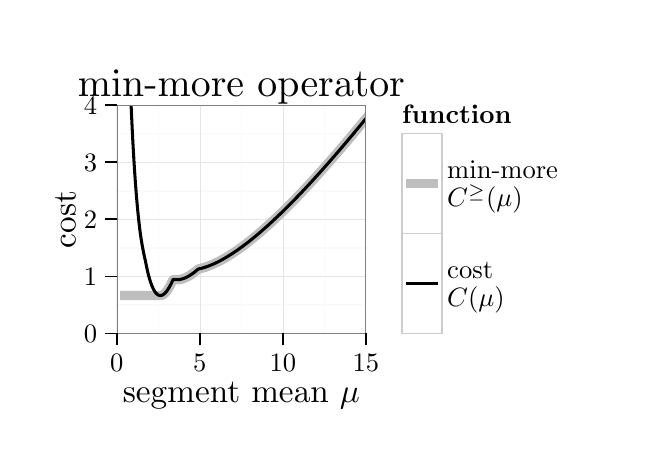
\begin{tikzpicture}[x=1pt,y=1pt]
\definecolor{fillColor}{RGB}{255,255,255}
\path[use as bounding box,fill=fillColor,fill opacity=0.00] (0,0) rectangle (216.81,144.54);
\begin{scope}
\path[clip] (  0.00,  0.00) rectangle (216.81,144.54);
\definecolor{drawColor}{RGB}{255,255,255}
\definecolor{fillColor}{RGB}{255,255,255}

\path[draw=drawColor,line width= 0.6pt,line join=round,line cap=round,fill=fillColor] (  0.00, -0.00) rectangle (216.81,144.54);
\end{scope}
\begin{scope}
\path[clip] ( 32.22, 34.03) rectangle (122.22,116.55);
\definecolor{fillColor}{RGB}{255,255,255}

\path[fill=fillColor] ( 32.22, 34.03) rectangle (122.22,116.55);
\definecolor{drawColor}{gray}{0.98}

\path[draw=drawColor,line width= 0.6pt,line join=round] ( 32.22, 44.35) --
	(122.22, 44.35);

\path[draw=drawColor,line width= 0.6pt,line join=round] ( 32.22, 64.98) --
	(122.22, 64.98);

\path[draw=drawColor,line width= 0.6pt,line join=round] ( 32.22, 85.61) --
	(122.22, 85.61);

\path[draw=drawColor,line width= 0.6pt,line join=round] ( 32.22,106.24) --
	(122.22,106.24);

\path[draw=drawColor,line width= 0.6pt,line join=round] ( 47.22, 34.03) --
	( 47.22,116.55);

\path[draw=drawColor,line width= 0.6pt,line join=round] ( 77.22, 34.03) --
	( 77.22,116.55);

\path[draw=drawColor,line width= 0.6pt,line join=round] (107.22, 34.03) --
	(107.22,116.55);
\definecolor{drawColor}{gray}{0.90}

\path[draw=drawColor,line width= 0.2pt,line join=round] ( 32.22, 34.03) --
	(122.22, 34.03);

\path[draw=drawColor,line width= 0.2pt,line join=round] ( 32.22, 54.66) --
	(122.22, 54.66);

\path[draw=drawColor,line width= 0.2pt,line join=round] ( 32.22, 75.29) --
	(122.22, 75.29);

\path[draw=drawColor,line width= 0.2pt,line join=round] ( 32.22, 95.92) --
	(122.22, 95.92);

\path[draw=drawColor,line width= 0.2pt,line join=round] ( 32.22,116.55) --
	(122.22,116.55);

\path[draw=drawColor,line width= 0.2pt,line join=round] ( 32.22, 34.03) --
	( 32.22,116.55);

\path[draw=drawColor,line width= 0.2pt,line join=round] ( 62.22, 34.03) --
	( 62.22,116.55);

\path[draw=drawColor,line width= 0.2pt,line join=round] ( 92.22, 34.03) --
	( 92.22,116.55);

\path[draw=drawColor,line width= 0.2pt,line join=round] (122.22, 34.03) --
	(122.22,116.55);
\definecolor{drawColor}{RGB}{190,190,190}

\path[draw=drawColor,line width= 3.4pt,line join=round] ( 33.40, 47.76) --
	( 33.55, 47.76) --
	( 33.70, 47.76) --
	( 33.84, 47.76) --
	( 33.99, 47.76) --
	( 34.14, 47.76) --
	( 34.28, 47.76) --
	( 34.43, 47.76) --
	( 34.58, 47.76) --
	( 34.73, 47.76) --
	( 34.87, 47.76) --
	( 35.02, 47.76) --
	( 35.17, 47.76) --
	( 35.31, 47.76) --
	( 35.46, 47.76) --
	( 35.61, 47.76) --
	( 35.75, 47.76) --
	( 35.90, 47.76) --
	( 36.05, 47.76) --
	( 36.19, 47.76) --
	( 36.34, 47.76) --
	( 36.49, 47.76) --
	( 36.63, 47.76) --
	( 36.78, 47.76) --
	( 36.93, 47.76) --
	( 37.08, 47.76) --
	( 37.22, 47.76) --
	( 37.37, 47.76) --
	( 37.52, 47.76) --
	( 37.66, 47.76) --
	( 37.81, 47.76) --
	( 37.96, 47.76) --
	( 38.10, 47.76) --
	( 38.25, 47.76) --
	( 38.40, 47.76) --
	( 38.54, 47.76) --
	( 38.69, 47.76) --
	( 38.84, 47.76) --
	( 38.98, 47.76) --
	( 39.13, 47.76) --
	( 39.28, 47.76) --
	( 39.43, 47.76) --
	( 39.57, 47.76) --
	( 39.72, 47.76) --
	( 39.87, 47.76) --
	( 40.01, 47.76) --
	( 40.16, 47.76) --
	( 40.31, 47.76) --
	( 40.45, 47.76) --
	( 40.60, 47.76) --
	( 40.75, 47.76) --
	( 40.89, 47.76) --
	( 41.04, 47.76) --
	( 41.19, 47.76) --
	( 41.34, 47.76) --
	( 41.48, 47.76) --
	( 41.63, 47.76) --
	( 41.78, 47.76) --
	( 41.92, 47.76) --
	( 42.07, 47.76) --
	( 42.22, 47.76) --
	( 42.36, 47.76) --
	( 42.51, 47.76) --
	( 42.66, 47.76) --
	( 42.80, 47.76) --
	( 42.95, 47.76) --
	( 43.10, 47.76) --
	( 43.24, 47.76) --
	( 43.39, 47.76) --
	( 43.54, 47.76) --
	( 43.69, 47.76) --
	( 43.83, 47.76) --
	( 43.98, 47.76) --
	( 44.13, 47.76) --
	( 44.27, 47.76) --
	( 44.42, 47.76) --
	( 44.57, 47.76) --
	( 44.71, 47.76) --
	( 44.86, 47.76) --
	( 45.01, 47.76) --
	( 45.15, 47.76) --
	( 45.30, 47.76) --
	( 45.45, 47.76) --
	( 45.59, 47.76) --
	( 45.74, 47.76) --
	( 45.89, 47.76) --
	( 46.04, 47.76) --
	( 46.18, 47.76) --
	( 46.33, 47.76) --
	( 46.48, 47.76) --
	( 46.62, 47.76) --
	( 46.77, 47.76) --
	( 46.92, 47.76) --
	( 47.06, 47.76) --
	( 47.21, 47.76) --
	( 47.36, 47.76) --
	( 47.50, 47.76) --
	( 47.65, 47.76) --
	( 47.80, 47.76) --
	( 47.94, 47.76) --
	( 47.94, 47.76) --
	( 47.99, 47.76) --
	( 48.04, 47.76) --
	( 48.08, 47.76) --
	( 48.13, 47.77) --
	( 48.17, 47.77) --
	( 48.22, 47.78) --
	( 48.27, 47.79) --
	( 48.31, 47.80) --
	( 48.36, 47.81) --
	( 48.40, 47.82) --
	( 48.45, 47.84) --
	( 48.50, 47.85) --
	( 48.54, 47.87) --
	( 48.59, 47.89) --
	( 48.63, 47.91) --
	( 48.68, 47.93) --
	( 48.73, 47.95) --
	( 48.77, 47.97) --
	( 48.82, 48.00) --
	( 48.86, 48.02) --
	( 48.91, 48.05) --
	( 48.95, 48.08) --
	( 49.00, 48.11) --
	( 49.05, 48.14) --
	( 49.09, 48.17) --
	( 49.14, 48.20) --
	( 49.18, 48.24) --
	( 49.23, 48.27) --
	( 49.28, 48.31) --
	( 49.32, 48.35) --
	( 49.37, 48.38) --
	( 49.41, 48.42) --
	( 49.46, 48.47) --
	( 49.51, 48.51) --
	( 49.55, 48.55) --
	( 49.60, 48.60) --
	( 49.64, 48.64) --
	( 49.69, 48.69) --
	( 49.74, 48.74) --
	( 49.78, 48.78) --
	( 49.83, 48.83) --
	( 49.87, 48.89) --
	( 49.92, 48.94) --
	( 49.97, 48.99) --
	( 50.01, 49.05) --
	( 50.06, 49.10) --
	( 50.10, 49.16) --
	( 50.15, 49.22) --
	( 50.19, 49.27) --
	( 50.24, 49.33) --
	( 50.29, 49.40) --
	( 50.33, 49.46) --
	( 50.38, 49.52) --
	( 50.42, 49.58) --
	( 50.47, 49.65) --
	( 50.52, 49.72) --
	( 50.56, 49.78) --
	( 50.61, 49.85) --
	( 50.65, 49.92) --
	( 50.70, 49.99) --
	( 50.75, 50.06) --
	( 50.79, 50.13) --
	( 50.84, 50.21) --
	( 50.88, 50.28) --
	( 50.93, 50.36) --
	( 50.98, 50.43) --
	( 51.02, 50.51) --
	( 51.07, 50.59) --
	( 51.11, 50.67) --
	( 51.16, 50.75) --
	( 51.21, 50.83) --
	( 51.25, 50.91) --
	( 51.30, 50.99) --
	( 51.34, 51.07) --
	( 51.39, 51.16) --
	( 51.43, 51.25) --
	( 51.48, 51.33) --
	( 51.53, 51.42) --
	( 51.57, 51.51) --
	( 51.62, 51.60) --
	( 51.66, 51.69) --
	( 51.71, 51.78) --
	( 51.76, 51.87) --
	( 51.80, 51.96) --
	( 51.85, 52.06) --
	( 51.89, 52.15) --
	( 51.94, 52.25) --
	( 51.99, 52.34) --
	( 52.03, 52.44) --
	( 52.08, 52.54) --
	( 52.12, 52.64) --
	( 52.17, 52.74) --
	( 52.22, 52.84) --
	( 52.26, 52.94) --
	( 52.31, 53.04) --
	( 52.35, 53.15) --
	( 52.40, 53.25) --
	( 52.45, 53.35) --
	( 52.49, 53.46) --
	( 52.49, 53.46) --
	( 52.50, 53.46) --
	( 52.52, 53.46) --
	( 52.53, 53.46) --
	( 52.55, 53.46) --
	( 52.56, 53.46) --
	( 52.57, 53.46) --
	( 52.59, 53.46) --
	( 52.60, 53.46) --
	( 52.62, 53.46) --
	( 52.63, 53.46) --
	( 52.64, 53.46) --
	( 52.66, 53.46) --
	( 52.67, 53.46) --
	( 52.68, 53.46) --
	( 52.70, 53.46) --
	( 52.71, 53.46) --
	( 52.73, 53.46) --
	( 52.74, 53.46) --
	( 52.75, 53.46) --
	( 52.77, 53.46) --
	( 52.78, 53.46) --
	( 52.80, 53.46) --
	( 52.81, 53.46) --
	( 52.82, 53.46) --
	( 52.84, 53.46) --
	( 52.85, 53.46) --
	( 52.86, 53.46) --
	( 52.88, 53.46) --
	( 52.89, 53.46) --
	( 52.91, 53.46) --
	( 52.92, 53.46) --
	( 52.93, 53.46) --
	( 52.95, 53.46) --
	( 52.96, 53.46) --
	( 52.97, 53.46) --
	( 52.99, 53.46) --
	( 53.00, 53.46) --
	( 53.02, 53.46) --
	( 53.03, 53.46) --
	( 53.04, 53.46) --
	( 53.06, 53.46) --
	( 53.07, 53.46) --
	( 53.09, 53.46) --
	( 53.10, 53.46) --
	( 53.11, 53.46) --
	( 53.13, 53.46) --
	( 53.14, 53.46) --
	( 53.15, 53.46) --
	( 53.17, 53.46) --
	( 53.18, 53.46) --
	( 53.20, 53.46) --
	( 53.21, 53.46) --
	( 53.22, 53.46) --
	( 53.24, 53.46) --
	( 53.25, 53.46) --
	( 53.26, 53.46) --
	( 53.28, 53.46) --
	( 53.29, 53.46) --
	( 53.31, 53.46) --
	( 53.32, 53.46) --
	( 53.33, 53.46) --
	( 53.35, 53.46) --
	( 53.36, 53.46) --
	( 53.38, 53.46) --
	( 53.39, 53.46) --
	( 53.40, 53.46) --
	( 53.42, 53.46) --
	( 53.43, 53.46) --
	( 53.44, 53.46) --
	( 53.46, 53.46) --
	( 53.47, 53.46) --
	( 53.49, 53.46) --
	( 53.50, 53.46) --
	( 53.51, 53.46) --
	( 53.53, 53.46) --
	( 53.54, 53.46) --
	( 53.56, 53.46) --
	( 53.57, 53.46) --
	( 53.58, 53.46) --
	( 53.60, 53.46) --
	( 53.61, 53.46) --
	( 53.62, 53.46) --
	( 53.64, 53.46) --
	( 53.65, 53.46) --
	( 53.67, 53.46) --
	( 53.68, 53.46) --
	( 53.69, 53.46) --
	( 53.71, 53.46) --
	( 53.72, 53.46) --
	( 53.73, 53.46) --
	( 53.75, 53.46) --
	( 53.76, 53.46) --
	( 53.78, 53.46) --
	( 53.79, 53.46) --
	( 53.80, 53.46) --
	( 53.82, 53.46) --
	( 53.83, 53.46) --
	( 53.85, 53.46) --
	( 53.86, 53.46) --
	( 53.86, 53.46) --
	( 53.94, 53.46) --
	( 54.02, 53.46) --
	( 54.09, 53.47) --
	( 54.17, 53.47) --
	( 54.25, 53.47) --
	( 54.33, 53.48) --
	( 54.41, 53.48) --
	( 54.48, 53.49) --
	( 54.56, 53.50) --
	( 54.64, 53.51) --
	( 54.72, 53.52) --
	( 54.80, 53.53) --
	( 54.87, 53.54) --
	( 54.95, 53.55) --
	( 55.03, 53.57) --
	( 55.11, 53.58) --
	( 55.19, 53.60) --
	( 55.26, 53.61) --
	( 55.34, 53.63) --
	( 55.42, 53.65) --
	( 55.50, 53.66) --
	( 55.58, 53.68) --
	( 55.65, 53.70) --
	( 55.73, 53.72) --
	( 55.81, 53.75) --
	( 55.89, 53.77) --
	( 55.97, 53.79) --
	( 56.04, 53.82) --
	( 56.12, 53.84) --
	( 56.20, 53.87) --
	( 56.28, 53.89) --
	( 56.36, 53.92) --
	( 56.43, 53.95) --
	( 56.51, 53.98) --
	( 56.59, 54.01) --
	( 56.67, 54.04) --
	( 56.75, 54.07) --
	( 56.82, 54.10) --
	( 56.90, 54.13) --
	( 56.98, 54.17) --
	( 57.06, 54.20) --
	( 57.14, 54.24) --
	( 57.21, 54.27) --
	( 57.29, 54.31) --
	( 57.37, 54.35) --
	( 57.45, 54.38) --
	( 57.53, 54.42) --
	( 57.60, 54.46) --
	( 57.68, 54.50) --
	( 57.76, 54.54) --
	( 57.84, 54.58) --
	( 57.92, 54.62) --
	( 57.99, 54.67) --
	( 58.07, 54.71) --
	( 58.15, 54.75) --
	( 58.23, 54.80) --
	( 58.31, 54.84) --
	( 58.38, 54.89) --
	( 58.46, 54.94) --
	( 58.54, 54.98) --
	( 58.62, 55.03) --
	( 58.70, 55.08) --
	( 58.77, 55.13) --
	( 58.85, 55.18) --
	( 58.93, 55.23) --
	( 59.01, 55.28) --
	( 59.09, 55.33) --
	( 59.16, 55.39) --
	( 59.24, 55.44) --
	( 59.32, 55.49) --
	( 59.40, 55.55) --
	( 59.48, 55.60) --
	( 59.55, 55.66) --
	( 59.63, 55.72) --
	( 59.71, 55.77) --
	( 59.79, 55.83) --
	( 59.87, 55.89) --
	( 59.94, 55.95) --
	( 60.02, 56.00) --
	( 60.10, 56.06) --
	( 60.18, 56.13) --
	( 60.26, 56.19) --
	( 60.33, 56.25) --
	( 60.41, 56.31) --
	( 60.49, 56.37) --
	( 60.57, 56.44) --
	( 60.65, 56.50) --
	( 60.72, 56.56) --
	( 60.80, 56.63) --
	( 60.88, 56.69) --
	( 60.96, 56.76) --
	( 61.04, 56.83) --
	( 61.11, 56.89) --
	( 61.19, 56.96) --
	( 61.27, 57.03) --
	( 61.35, 57.10) --
	( 61.43, 57.17) --
	( 61.50, 57.24) --
	( 61.58, 57.31) --
	( 61.58, 57.31) --
	( 62.58, 57.54) --
	( 63.58, 57.81) --
	( 64.59, 58.14) --
	( 65.59, 58.50) --
	( 66.59, 58.91) --
	( 67.59, 59.35) --
	( 68.59, 59.83) --
	( 69.60, 60.34) --
	( 70.60, 60.89) --
	( 71.60, 61.46) --
	( 72.60, 62.07) --
	( 73.60, 62.70) --
	( 74.60, 63.36) --
	( 75.61, 64.04) --
	( 76.61, 64.75) --
	( 77.61, 65.47) --
	( 78.61, 66.23) --
	( 79.61, 67.00) --
	( 80.62, 67.79) --
	( 81.62, 68.60) --
	( 82.62, 69.43) --
	( 83.62, 70.27) --
	( 84.62, 71.14) --
	( 85.62, 72.02) --
	( 86.63, 72.91) --
	( 87.63, 73.82) --
	( 88.63, 74.75) --
	( 89.63, 75.69) --
	( 90.63, 76.64) --
	( 91.63, 77.60) --
	( 92.64, 78.58) --
	( 93.64, 79.57) --
	( 94.64, 80.57) --
	( 95.64, 81.59) --
	( 96.64, 82.61) --
	( 97.65, 83.65) --
	( 98.65, 84.69) --
	( 99.65, 85.75) --
	(100.65, 86.82) --
	(101.65, 87.89) --
	(102.65, 88.98) --
	(103.66, 90.07) --
	(104.66, 91.17) --
	(105.66, 92.28) --
	(106.66, 93.40) --
	(107.66, 94.53) --
	(108.66, 95.66) --
	(109.67, 96.81) --
	(110.67, 97.96) --
	(111.67, 99.12) --
	(112.67,100.28) --
	(113.67,101.45) --
	(114.68,102.63) --
	(115.68,103.81) --
	(116.68,105.01) --
	(117.68,106.20) --
	(118.68,107.41) --
	(119.68,108.62) --
	(120.69,109.83) --
	(121.69,111.05) --
	(122.69,112.28) --
	(123.69,113.51) --
	(124.69,114.75) --
	(125.69,115.99) --
	(126.70,117.24) --
	(127.70,118.49) --
	(128.70,119.75) --
	(129.70,121.01) --
	(130.70,122.28) --
	(131.71,123.55) --
	(132.71,124.83) --
	(133.71,126.11) --
	(134.71,127.39) --
	(135.71,128.68) --
	(136.71,129.98) --
	(137.72,131.28) --
	(138.72,132.58) --
	(139.72,133.88) --
	(140.72,135.19) --
	(141.72,136.51) --
	(142.73,137.82) --
	(143.73,139.14) --
	(144.73,140.47) --
	(145.73,141.80) --
	(146.73,143.13) --
	(147.73,144.46) --
	(147.79,144.54);
\definecolor{drawColor}{RGB}{0,0,0}

\path[draw=drawColor,line width= 1.1pt,line join=round] ( 36.37,144.54) --
	( 36.37,144.21) --
	( 36.45,141.63) --
	( 36.53,139.12) --
	( 36.61,136.68) --
	( 36.69,134.31) --
	( 36.77,132.01) --
	( 36.85,129.77) --
	( 36.93,127.59) --
	( 37.01,125.48) --
	( 37.09,123.42) --
	( 37.17,121.41) --
	( 37.25,119.46) --
	( 37.33,117.56) --
	( 37.41,115.72) --
	( 37.49,113.92) --
	( 37.57,112.17) --
	( 37.65,110.46) --
	( 37.73,108.80) --
	( 37.81,107.19) --
	( 37.89,105.61) --
	( 37.97,104.08) --
	( 38.05,102.59) --
	( 38.13,101.14) --
	( 38.21, 99.72) --
	( 38.29, 98.34) --
	( 38.37, 97.00) --
	( 38.45, 95.69) --
	( 38.53, 94.42) --
	( 38.61, 93.18) --
	( 38.69, 91.97) --
	( 38.77, 90.79) --
	( 38.85, 89.65) --
	( 38.93, 88.53) --
	( 39.01, 87.45) --
	( 39.09, 86.39) --
	( 39.17, 85.36) --
	( 39.25, 84.36) --
	( 39.33, 83.39) --
	( 39.41, 82.44) --
	( 39.49, 81.52) --
	( 39.57, 80.62) --
	( 39.65, 79.74) --
	( 39.73, 78.90) --
	( 39.81, 78.07) --
	( 39.89, 77.27) --
	( 39.97, 76.49) --
	( 40.05, 75.73) --
	( 40.13, 74.99) --
	( 40.21, 74.28) --
	( 40.29, 73.58) --
	( 40.37, 72.91) --
	( 40.44, 72.25) --
	( 40.52, 71.62) --
	( 40.60, 71.00) --
	( 40.68, 70.41) --
	( 40.76, 69.83) --
	( 40.84, 69.27) --
	( 40.92, 68.73) --
	( 41.00, 68.20) --
	( 41.08, 67.69) --
	( 41.16, 67.20) --
	( 41.24, 66.73) --
	( 41.32, 66.27) --
	( 41.40, 65.83) --
	( 41.48, 65.40) --
	( 41.56, 64.99) --
	( 41.56, 64.99) --
	( 41.57, 64.93) --
	( 41.58, 64.88) --
	( 41.59, 64.82) --
	( 41.60, 64.76) --
	( 41.61, 64.71) --
	( 41.62, 64.65) --
	( 41.63, 64.59) --
	( 41.64, 64.54) --
	( 41.65, 64.48) --
	( 41.66, 64.43) --
	( 41.67, 64.37) --
	( 41.68, 64.32) --
	( 41.69, 64.26) --
	( 41.70, 64.21) --
	( 41.71, 64.15) --
	( 41.72, 64.10) --
	( 41.73, 64.04) --
	( 41.74, 63.99) --
	( 41.75, 63.94) --
	( 41.76, 63.88) --
	( 41.77, 63.83) --
	( 41.78, 63.78) --
	( 41.79, 63.72) --
	( 41.80, 63.67) --
	( 41.81, 63.62) --
	( 41.82, 63.57) --
	( 41.83, 63.52) --
	( 41.84, 63.46) --
	( 41.85, 63.41) --
	( 41.86, 63.36) --
	( 41.87, 63.31) --
	( 41.88, 63.26) --
	( 41.89, 63.21) --
	( 41.90, 63.16) --
	( 41.91, 63.11) --
	( 41.92, 63.06) --
	( 41.93, 63.01) --
	( 41.94, 62.96) --
	( 41.95, 62.91) --
	( 41.96, 62.86) --
	( 41.97, 62.81) --
	( 41.98, 62.76) --
	( 41.99, 62.71) --
	( 42.00, 62.67) --
	( 42.01, 62.62) --
	( 42.02, 62.57) --
	( 42.03, 62.52) --
	( 42.04, 62.48) --
	( 42.05, 62.43) --
	( 42.06, 62.38) --
	( 42.07, 62.33) --
	( 42.08, 62.29) --
	( 42.09, 62.24) --
	( 42.10, 62.19) --
	( 42.11, 62.15) --
	( 42.12, 62.10) --
	( 42.13, 62.06) --
	( 42.14, 62.01) --
	( 42.15, 61.97) --
	( 42.16, 61.92) --
	( 42.17, 61.88) --
	( 42.18, 61.83) --
	( 42.19, 61.79) --
	( 42.20, 61.74) --
	( 42.21, 61.70) --
	( 42.22, 61.65) --
	( 42.22, 61.61) --
	( 42.23, 61.57) --
	( 42.24, 61.52) --
	( 42.25, 61.48) --
	( 42.26, 61.44) --
	( 42.27, 61.39) --
	( 42.28, 61.35) --
	( 42.29, 61.31) --
	( 42.30, 61.27) --
	( 42.31, 61.23) --
	( 42.32, 61.18) --
	( 42.33, 61.14) --
	( 42.34, 61.10) --
	( 42.35, 61.06) --
	( 42.36, 61.02) --
	( 42.37, 60.98) --
	( 42.38, 60.94) --
	( 42.39, 60.90) --
	( 42.40, 60.86) --
	( 42.41, 60.82) --
	( 42.42, 60.78) --
	( 42.43, 60.74) --
	( 42.44, 60.70) --
	( 42.45, 60.66) --
	( 42.46, 60.62) --
	( 42.47, 60.58) --
	( 42.48, 60.54) --
	( 42.49, 60.50) --
	( 42.50, 60.46) --
	( 42.51, 60.43) --
	( 42.52, 60.39) --
	( 42.53, 60.35) --
	( 42.54, 60.31) --
	( 42.54, 60.31) --
	( 42.64, 59.77) --
	( 42.74, 59.25) --
	( 42.84, 58.74) --
	( 42.95, 58.25) --
	( 43.05, 57.77) --
	( 43.15, 57.31) --
	( 43.25, 56.85) --
	( 43.35, 56.42) --
	( 43.45, 55.99) --
	( 43.55, 55.58) --
	( 43.65, 55.18) --
	( 43.75, 54.80) --
	( 43.86, 54.43) --
	( 43.96, 54.07) --
	( 44.06, 53.72) --
	( 44.16, 53.38) --
	( 44.26, 53.06) --
	( 44.36, 52.74) --
	( 44.46, 52.44) --
	( 44.56, 52.15) --
	( 44.66, 51.87) --
	( 44.77, 51.60) --
	( 44.87, 51.34) --
	( 44.97, 51.09) --
	( 45.07, 50.85) --
	( 45.17, 50.62) --
	( 45.27, 50.41) --
	( 45.37, 50.20) --
	( 45.47, 50.00) --
	( 45.57, 49.81) --
	( 45.68, 49.63) --
	( 45.78, 49.46) --
	( 45.88, 49.29) --
	( 45.98, 49.14) --
	( 46.08, 49.00) --
	( 46.18, 48.86) --
	( 46.28, 48.73) --
	( 46.38, 48.61) --
	( 46.48, 48.50) --
	( 46.59, 48.40) --
	( 46.69, 48.30) --
	( 46.79, 48.22) --
	( 46.89, 48.14) --
	( 46.99, 48.07) --
	( 47.09, 48.00) --
	( 47.19, 47.95) --
	( 47.29, 47.90) --
	( 47.40, 47.86) --
	( 47.50, 47.82) --
	( 47.60, 47.80) --
	( 47.70, 47.78) --
	( 47.80, 47.76) --
	( 47.90, 47.76) --
	( 48.00, 47.76) --
	( 48.10, 47.77) --
	( 48.20, 47.78) --
	( 48.31, 47.80) --
	( 48.41, 47.83) --
	( 48.51, 47.86) --
	( 48.61, 47.90) --
	( 48.71, 47.94) --
	( 48.81, 47.99) --
	( 48.91, 48.05) --
	( 49.01, 48.12) --
	( 49.11, 48.18) --
	( 49.22, 48.26) --
	( 49.32, 48.34) --
	( 49.42, 48.43) --
	( 49.52, 48.52) --
	( 49.62, 48.62) --
	( 49.72, 48.72) --
	( 49.82, 48.83) --
	( 49.92, 48.94) --
	( 50.02, 49.06) --
	( 50.13, 49.19) --
	( 50.23, 49.32) --
	( 50.33, 49.45) --
	( 50.43, 49.59) --
	( 50.53, 49.73) --
	( 50.63, 49.88) --
	( 50.73, 50.04) --
	( 50.83, 50.20) --
	( 50.93, 50.36) --
	( 51.04, 50.53) --
	( 51.14, 50.71) --
	( 51.24, 50.88) --
	( 51.34, 51.07) --
	( 51.44, 51.25) --
	( 51.54, 51.45) --
	( 51.64, 51.64) --
	( 51.74, 51.84) --
	( 51.84, 52.05) --
	( 51.95, 52.26) --
	( 52.05, 52.47) --
	( 52.15, 52.69) --
	( 52.25, 52.91) --
	( 52.35, 53.14) --
	( 52.45, 53.37) --
	( 52.55, 53.60) --
	( 52.55, 53.60) --
	( 52.64, 53.58) --
	( 52.73, 53.57) --
	( 52.83, 53.55) --
	( 52.92, 53.53) --
	( 53.01, 53.52) --
	( 53.10, 53.51) --
	( 53.19, 53.50) --
	( 53.28, 53.49) --
	( 53.37, 53.48) --
	( 53.46, 53.47) --
	( 53.56, 53.47) --
	( 53.65, 53.46) --
	( 53.74, 53.46) --
	( 53.83, 53.46) --
	( 53.92, 53.46) --
	( 54.01, 53.46) --
	( 54.10, 53.47) --
	( 54.19, 53.47) --
	( 54.28, 53.48) --
	( 54.38, 53.48) --
	( 54.47, 53.49) --
	( 54.56, 53.50) --
	( 54.65, 53.51) --
	( 54.74, 53.52) --
	( 54.83, 53.53) --
	( 54.92, 53.55) --
	( 55.01, 53.56) --
	( 55.11, 53.58) --
	( 55.20, 53.60) --
	( 55.29, 53.62) --
	( 55.38, 53.64) --
	( 55.47, 53.66) --
	( 55.56, 53.68) --
	( 55.65, 53.70) --
	( 55.74, 53.73) --
	( 55.84, 53.75) --
	( 55.93, 53.78) --
	( 56.02, 53.81) --
	( 56.11, 53.84) --
	( 56.20, 53.87) --
	( 56.29, 53.90) --
	( 56.38, 53.93) --
	( 56.47, 53.96) --
	( 56.56, 54.00) --
	( 56.66, 54.03) --
	( 56.75, 54.07) --
	( 56.84, 54.11) --
	( 56.93, 54.15) --
	( 57.02, 54.19) --
	( 57.11, 54.23) --
	( 57.20, 54.27) --
	( 57.29, 54.31) --
	( 57.39, 54.35) --
	( 57.48, 54.40) --
	( 57.57, 54.44) --
	( 57.66, 54.49) --
	( 57.75, 54.54) --
	( 57.84, 54.59) --
	( 57.93, 54.63) --
	( 58.02, 54.68) --
	( 58.12, 54.74) --
	( 58.21, 54.79) --
	( 58.30, 54.84) --
	( 58.39, 54.89) --
	( 58.48, 54.95) --
	( 58.57, 55.00) --
	( 58.66, 55.06) --
	( 58.75, 55.12) --
	( 58.85, 55.18) --
	( 58.94, 55.24) --
	( 59.03, 55.30) --
	( 59.12, 55.36) --
	( 59.21, 55.42) --
	( 59.30, 55.48) --
	( 59.39, 55.54) --
	( 59.48, 55.61) --
	( 59.57, 55.67) --
	( 59.67, 55.74) --
	( 59.76, 55.81) --
	( 59.85, 55.87) --
	( 59.94, 55.94) --
	( 60.03, 56.01) --
	( 60.12, 56.08) --
	( 60.21, 56.15) --
	( 60.30, 56.22) --
	( 60.40, 56.30) --
	( 60.49, 56.37) --
	( 60.58, 56.44) --
	( 60.67, 56.52) --
	( 60.76, 56.59) --
	( 60.85, 56.67) --
	( 60.94, 56.75) --
	( 61.03, 56.83) --
	( 61.13, 56.90) --
	( 61.22, 56.98) --
	( 61.31, 57.06) --
	( 61.40, 57.14) --
	( 61.49, 57.22) --
	( 61.58, 57.31) --
	( 61.58, 57.31) --
	( 62.58, 57.54) --
	( 63.58, 57.81) --
	( 64.59, 58.14) --
	( 65.59, 58.50) --
	( 66.59, 58.91) --
	( 67.59, 59.35) --
	( 68.59, 59.83) --
	( 69.60, 60.34) --
	( 70.60, 60.89) --
	( 71.60, 61.46) --
	( 72.60, 62.07) --
	( 73.60, 62.70) --
	( 74.60, 63.36) --
	( 75.61, 64.04) --
	( 76.61, 64.75) --
	( 77.61, 65.47) --
	( 78.61, 66.23) --
	( 79.61, 67.00) --
	( 80.62, 67.79) --
	( 81.62, 68.60) --
	( 82.62, 69.43) --
	( 83.62, 70.27) --
	( 84.62, 71.14) --
	( 85.62, 72.02) --
	( 86.63, 72.91) --
	( 87.63, 73.82) --
	( 88.63, 74.75) --
	( 89.63, 75.69) --
	( 90.63, 76.64) --
	( 91.63, 77.60) --
	( 92.64, 78.58) --
	( 93.64, 79.57) --
	( 94.64, 80.57) --
	( 95.64, 81.59) --
	( 96.64, 82.61) --
	( 97.65, 83.65) --
	( 98.65, 84.69) --
	( 99.65, 85.75) --
	(100.65, 86.82) --
	(101.65, 87.89) --
	(102.65, 88.98) --
	(103.66, 90.07) --
	(104.66, 91.17) --
	(105.66, 92.28) --
	(106.66, 93.40) --
	(107.66, 94.53) --
	(108.66, 95.66) --
	(109.67, 96.81) --
	(110.67, 97.96) --
	(111.67, 99.12) --
	(112.67,100.28) --
	(113.67,101.45) --
	(114.68,102.63) --
	(115.68,103.81) --
	(116.68,105.01) --
	(117.68,106.20) --
	(118.68,107.41) --
	(119.68,108.62) --
	(120.69,109.83) --
	(121.69,111.05) --
	(122.69,112.28) --
	(123.69,113.51) --
	(124.69,114.75) --
	(125.69,115.99) --
	(126.70,117.24) --
	(127.70,118.49) --
	(128.70,119.75) --
	(129.70,121.01) --
	(130.70,122.28) --
	(131.71,123.55) --
	(132.71,124.83) --
	(133.71,126.11) --
	(134.71,127.39) --
	(135.71,128.68) --
	(136.71,129.98) --
	(137.72,131.28) --
	(138.72,132.58) --
	(139.72,133.88) --
	(140.72,135.19) --
	(141.72,136.51) --
	(142.73,137.82) --
	(143.73,139.14) --
	(144.73,140.47) --
	(145.73,141.80) --
	(146.73,143.13) --
	(147.73,144.46) --
	(147.79,144.54);
\definecolor{drawColor}{gray}{0.50}

\path[draw=drawColor,line width= 0.6pt,line join=round,line cap=round] ( 32.22, 34.03) rectangle (122.22,116.55);
\end{scope}
\begin{scope}
\path[clip] (  0.00,  0.00) rectangle (216.81,144.54);
\definecolor{drawColor}{RGB}{0,0,0}

\node[text=drawColor,anchor=base east,inner sep=0pt, outer sep=0pt, scale=  0.96] at ( 25.11, 30.73) {0};

\node[text=drawColor,anchor=base east,inner sep=0pt, outer sep=0pt, scale=  0.96] at ( 25.11, 51.36) {1};

\node[text=drawColor,anchor=base east,inner sep=0pt, outer sep=0pt, scale=  0.96] at ( 25.11, 71.99) {2};

\node[text=drawColor,anchor=base east,inner sep=0pt, outer sep=0pt, scale=  0.96] at ( 25.11, 92.62) {3};

\node[text=drawColor,anchor=base east,inner sep=0pt, outer sep=0pt, scale=  0.96] at ( 25.11,113.25) {4};
\end{scope}
\begin{scope}
\path[clip] (  0.00,  0.00) rectangle (216.81,144.54);
\definecolor{drawColor}{RGB}{0,0,0}

\path[draw=drawColor,line width= 0.6pt,line join=round] ( 27.95, 34.03) --
	( 32.22, 34.03);

\path[draw=drawColor,line width= 0.6pt,line join=round] ( 27.95, 54.66) --
	( 32.22, 54.66);

\path[draw=drawColor,line width= 0.6pt,line join=round] ( 27.95, 75.29) --
	( 32.22, 75.29);

\path[draw=drawColor,line width= 0.6pt,line join=round] ( 27.95, 95.92) --
	( 32.22, 95.92);

\path[draw=drawColor,line width= 0.6pt,line join=round] ( 27.95,116.55) --
	( 32.22,116.55);
\end{scope}
\begin{scope}
\path[clip] (  0.00,  0.00) rectangle (216.81,144.54);
\definecolor{drawColor}{RGB}{0,0,0}

\path[draw=drawColor,line width= 0.6pt,line join=round] ( 32.22, 29.77) --
	( 32.22, 34.03);

\path[draw=drawColor,line width= 0.6pt,line join=round] ( 62.22, 29.77) --
	( 62.22, 34.03);

\path[draw=drawColor,line width= 0.6pt,line join=round] ( 92.22, 29.77) --
	( 92.22, 34.03);

\path[draw=drawColor,line width= 0.6pt,line join=round] (122.22, 29.77) --
	(122.22, 34.03);
\end{scope}
\begin{scope}
\path[clip] (  0.00,  0.00) rectangle (216.81,144.54);
\definecolor{drawColor}{RGB}{0,0,0}

\node[text=drawColor,anchor=base,inner sep=0pt, outer sep=0pt, scale=  0.96] at ( 32.22, 20.31) {0};

\node[text=drawColor,anchor=base,inner sep=0pt, outer sep=0pt, scale=  0.96] at ( 62.22, 20.31) {5};

\node[text=drawColor,anchor=base,inner sep=0pt, outer sep=0pt, scale=  0.96] at ( 92.22, 20.31) {10};

\node[text=drawColor,anchor=base,inner sep=0pt, outer sep=0pt, scale=  0.96] at (122.22, 20.31) {15};
\end{scope}
\begin{scope}
\path[clip] (  0.00,  0.00) rectangle (216.81,144.54);
\definecolor{drawColor}{RGB}{0,0,0}

\node[text=drawColor,anchor=base,inner sep=0pt, outer sep=0pt, scale=  1.20] at ( 77.22,  9.03) {segment mean $\mu$};
\end{scope}
\begin{scope}
\path[clip] (  0.00,  0.00) rectangle (216.81,144.54);
\definecolor{drawColor}{RGB}{0,0,0}

\node[text=drawColor,rotate= 90.00,anchor=base,inner sep=0pt, outer sep=0pt, scale=  1.20] at ( 17.30, 75.29) {cost};
\end{scope}
\begin{scope}
\path[clip] (  0.00,  0.00) rectangle (216.81,144.54);
\definecolor{fillColor}{RGB}{255,255,255}

\path[fill=fillColor] (131.08, 29.77) rectangle (195.90,120.82);
\end{scope}
\begin{scope}
\path[clip] (  0.00,  0.00) rectangle (216.81,144.54);
\definecolor{drawColor}{RGB}{0,0,0}

\node[text=drawColor,anchor=base west,inner sep=0pt, outer sep=0pt, scale=  0.96] at (135.35,109.92) {\bfseries function};
\end{scope}
\begin{scope}
\path[clip] (  0.00,  0.00) rectangle (216.81,144.54);
\definecolor{drawColor}{gray}{0.80}
\definecolor{fillColor}{RGB}{255,255,255}

\path[draw=drawColor,line width= 0.6pt,line join=round,line cap=round,fill=fillColor] (135.35, 70.18) rectangle (149.81,106.31);
\end{scope}
\begin{scope}
\path[clip] (  0.00,  0.00) rectangle (216.81,144.54);
\definecolor{drawColor}{RGB}{190,190,190}

\path[draw=drawColor,line width= 3.4pt,line join=round] (136.80, 88.24) -- (148.36, 88.24);
\end{scope}
\begin{scope}
\path[clip] (  0.00,  0.00) rectangle (216.81,144.54);
\definecolor{drawColor}{gray}{0.80}
\definecolor{fillColor}{RGB}{255,255,255}

\path[draw=drawColor,line width= 0.6pt,line join=round,line cap=round,fill=fillColor] (135.35, 34.04) rectangle (149.81, 70.18);
\end{scope}
\begin{scope}
\path[clip] (  0.00,  0.00) rectangle (216.81,144.54);
\definecolor{drawColor}{RGB}{0,0,0}

\path[draw=drawColor,line width= 1.1pt,line join=round] (136.80, 52.11) -- (148.36, 52.11);
\end{scope}
\begin{scope}
\path[clip] (  0.00,  0.00) rectangle (216.81,144.54);
\definecolor{drawColor}{RGB}{0,0,0}

\node[text=drawColor,anchor=base west,inner sep=0pt, outer sep=0pt, scale=  0.96] at (151.61, 90.12) {min-more};

\node[text=drawColor,anchor=base west,inner sep=0pt, outer sep=0pt, scale=  0.96] at (151.61, 79.75) {$C^{\geq}(\mu)$};
\end{scope}
\begin{scope}
\path[clip] (  0.00,  0.00) rectangle (216.81,144.54);
\definecolor{drawColor}{RGB}{0,0,0}

\node[text=drawColor,anchor=base west,inner sep=0pt, outer sep=0pt, scale=  0.96] at (151.61, 53.99) {cost};

\node[text=drawColor,anchor=base west,inner sep=0pt, outer sep=0pt, scale=  0.96] at (151.61, 43.62) {$C(\mu)$};
\end{scope}
\begin{scope}
\path[clip] (  0.00,  0.00) rectangle (216.81,144.54);
\definecolor{drawColor}{RGB}{0,0,0}

\node[text=drawColor,anchor=base,inner sep=0pt, outer sep=0pt, scale=  1.44] at ( 77.22,119.57) {min-more operator};
\end{scope}
\end{tikzpicture}

    \end{center}
  }
  \parbox{3in}{
    \begin{center}
      % Created by tikzDevice version 0.7.0 on 2016-06-06 10:57:24
% !TEX encoding = UTF-8 Unicode
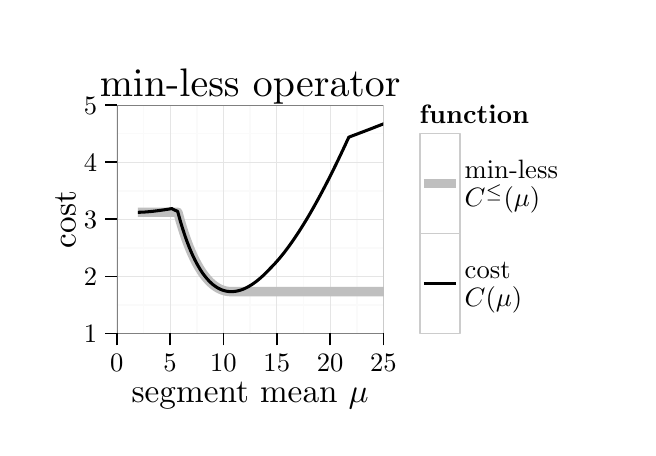
\begin{tikzpicture}[x=1pt,y=1pt]
\definecolor[named]{fillColor}{rgb}{1.00,1.00,1.00}
\path[use as bounding box,fill=fillColor,fill opacity=0.00] (0,0) rectangle (216.81,144.54);
\begin{scope}
\path[clip] (  0.00,  0.00) rectangle (216.81,144.54);
\definecolor[named]{drawColor}{rgb}{1.00,1.00,1.00}
\definecolor[named]{fillColor}{rgb}{1.00,1.00,1.00}

\path[draw=drawColor,line width= 0.6pt,line join=round,line cap=round,fill=fillColor] ( -0.00,  0.00) rectangle (216.81,144.54);
\end{scope}
\begin{scope}
\path[clip] ( 32.22, 34.03) rectangle (128.53,116.55);
\definecolor[named]{fillColor}{rgb}{1.00,1.00,1.00}

\path[fill=fillColor] ( 32.22, 34.03) rectangle (128.53,116.55);
\definecolor[named]{drawColor}{rgb}{0.98,0.98,0.98}

\path[draw=drawColor,line width= 0.6pt,line join=round] ( 32.22, 44.35) --
	(128.53, 44.35);

\path[draw=drawColor,line width= 0.6pt,line join=round] ( 32.22, 64.98) --
	(128.53, 64.98);

\path[draw=drawColor,line width= 0.6pt,line join=round] ( 32.22, 85.61) --
	(128.53, 85.61);

\path[draw=drawColor,line width= 0.6pt,line join=round] ( 32.22,106.24) --
	(128.53,106.24);

\path[draw=drawColor,line width= 0.6pt,line join=round] ( 41.85, 34.03) --
	( 41.85,116.55);

\path[draw=drawColor,line width= 0.6pt,line join=round] ( 61.12, 34.03) --
	( 61.12,116.55);

\path[draw=drawColor,line width= 0.6pt,line join=round] ( 80.38, 34.03) --
	( 80.38,116.55);

\path[draw=drawColor,line width= 0.6pt,line join=round] ( 99.64, 34.03) --
	( 99.64,116.55);

\path[draw=drawColor,line width= 0.6pt,line join=round] (118.90, 34.03) --
	(118.90,116.55);
\definecolor[named]{drawColor}{rgb}{0.90,0.90,0.90}

\path[draw=drawColor,line width= 0.2pt,line join=round] ( 32.22, 34.03) --
	(128.53, 34.03);

\path[draw=drawColor,line width= 0.2pt,line join=round] ( 32.22, 54.66) --
	(128.53, 54.66);

\path[draw=drawColor,line width= 0.2pt,line join=round] ( 32.22, 75.29) --
	(128.53, 75.29);

\path[draw=drawColor,line width= 0.2pt,line join=round] ( 32.22, 95.92) --
	(128.53, 95.92);

\path[draw=drawColor,line width= 0.2pt,line join=round] ( 32.22,116.55) --
	(128.53,116.55);

\path[draw=drawColor,line width= 0.2pt,line join=round] ( 32.22, 34.03) --
	( 32.22,116.55);

\path[draw=drawColor,line width= 0.2pt,line join=round] ( 51.48, 34.03) --
	( 51.48,116.55);

\path[draw=drawColor,line width= 0.2pt,line join=round] ( 70.75, 34.03) --
	( 70.75,116.55);

\path[draw=drawColor,line width= 0.2pt,line join=round] ( 90.01, 34.03) --
	( 90.01,116.55);

\path[draw=drawColor,line width= 0.2pt,line join=round] (109.27, 34.03) --
	(109.27,116.55);

\path[draw=drawColor,line width= 0.2pt,line join=round] (128.53, 34.03) --
	(128.53,116.55);
\definecolor[named]{drawColor}{rgb}{0.75,0.75,0.75}

\path[draw=drawColor,line width= 3.4pt,line join=round] ( 39.81, 77.83) --
	( 39.96, 77.83) --
	( 40.10, 77.83) --
	( 40.25, 77.83) --
	( 40.40, 77.83) --
	( 40.54, 77.83) --
	( 40.69, 77.83) --
	( 40.83, 77.83) --
	( 40.98, 77.83) --
	( 41.13, 77.83) --
	( 41.27, 77.83) --
	( 41.42, 77.83) --
	( 41.56, 77.83) --
	( 41.71, 77.83) --
	( 41.86, 77.83) --
	( 42.00, 77.83) --
	( 42.15, 77.83) --
	( 42.30, 77.83) --
	( 42.44, 77.83) --
	( 42.59, 77.83) --
	( 42.73, 77.83) --
	( 42.88, 77.83) --
	( 43.03, 77.83) --
	( 43.17, 77.83) --
	( 43.32, 77.83) --
	( 43.46, 77.83) --
	( 43.61, 77.83) --
	( 43.76, 77.83) --
	( 43.90, 77.83) --
	( 44.05, 77.83) --
	( 44.20, 77.83) --
	( 44.34, 77.83) --
	( 44.49, 77.83) --
	( 44.63, 77.83) --
	( 44.78, 77.83) --
	( 44.93, 77.83) --
	( 45.07, 77.83) --
	( 45.22, 77.83) --
	( 45.37, 77.83) --
	( 45.51, 77.83) --
	( 45.66, 77.83) --
	( 45.80, 77.83) --
	( 45.95, 77.83) --
	( 46.10, 77.83) --
	( 46.24, 77.83) --
	( 46.39, 77.83) --
	( 46.53, 77.83) --
	( 46.68, 77.83) --
	( 46.83, 77.83) --
	( 46.97, 77.83) --
	( 47.12, 77.83) --
	( 47.27, 77.83) --
	( 47.41, 77.83) --
	( 47.56, 77.83) --
	( 47.70, 77.83) --
	( 47.85, 77.83) --
	( 48.00, 77.83) --
	( 48.14, 77.83) --
	( 48.29, 77.83) --
	( 48.43, 77.83) --
	( 48.58, 77.83) --
	( 48.73, 77.83) --
	( 48.87, 77.83) --
	( 49.02, 77.83) --
	( 49.17, 77.83) --
	( 49.31, 77.83) --
	( 49.46, 77.83) --
	( 49.60, 77.83) --
	( 49.75, 77.83) --
	( 49.90, 77.83) --
	( 50.04, 77.83) --
	( 50.19, 77.83) --
	( 50.33, 77.83) --
	( 50.48, 77.83) --
	( 50.63, 77.83) --
	( 50.77, 77.83) --
	( 50.92, 77.83) --
	( 51.07, 77.83) --
	( 51.21, 77.83) --
	( 51.36, 77.83) --
	( 51.50, 77.83) --
	( 51.65, 77.83) --
	( 51.80, 77.83) --
	( 51.94, 77.83) --
	( 52.09, 77.83) --
	( 52.23, 77.83) --
	( 52.38, 77.83) --
	( 52.53, 77.83) --
	( 52.67, 77.83) --
	( 52.82, 77.83) --
	( 52.97, 77.83) --
	( 53.11, 77.83) --
	( 53.26, 77.83) --
	( 53.40, 77.83) --
	( 53.55, 77.83) --
	( 53.70, 77.83) --
	( 53.84, 77.83) --
	( 53.99, 77.83) --
	( 54.13, 77.83) --
	( 54.28, 77.83) --
	( 54.28, 77.83) --
	( 54.48, 77.11) --
	( 54.67, 76.40) --
	( 54.87, 75.70) --
	( 55.06, 75.02) --
	( 55.25, 74.35) --
	( 55.45, 73.69) --
	( 55.64, 73.05) --
	( 55.84, 72.41) --
	( 56.03, 71.79) --
	( 56.23, 71.18) --
	( 56.42, 70.58) --
	( 56.62, 70.00) --
	( 56.81, 69.42) --
	( 57.01, 68.86) --
	( 57.20, 68.31) --
	( 57.40, 67.77) --
	( 57.59, 67.24) --
	( 57.79, 66.72) --
	( 57.98, 66.20) --
	( 58.18, 65.70) --
	( 58.37, 65.21) --
	( 58.57, 64.73) --
	( 58.76, 64.26) --
	( 58.96, 63.80) --
	( 59.15, 63.35) --
	( 59.35, 62.91) --
	( 59.54, 62.47) --
	( 59.74, 62.05) --
	( 59.93, 61.64) --
	( 60.13, 61.23) --
	( 60.32, 60.83) --
	( 60.52, 60.44) --
	( 60.71, 60.06) --
	( 60.91, 59.69) --
	( 61.10, 59.32) --
	( 61.30, 58.97) --
	( 61.49, 58.62) --
	( 61.69, 58.28) --
	( 61.88, 57.94) --
	( 62.08, 57.62) --
	( 62.27, 57.30) --
	( 62.47, 56.99) --
	( 62.66, 56.69) --
	( 62.86, 56.39) --
	( 63.05, 56.10) --
	( 63.24, 55.82) --
	( 63.44, 55.55) --
	( 63.63, 55.28) --
	( 63.83, 55.02) --
	( 64.02, 54.77) --
	( 64.22, 54.52) --
	( 64.41, 54.28) --
	( 64.61, 54.04) --
	( 64.80, 53.81) --
	( 65.00, 53.59) --
	( 65.19, 53.38) --
	( 65.39, 53.17) --
	( 65.58, 52.97) --
	( 65.78, 52.77) --
	( 65.97, 52.58) --
	( 66.17, 52.39) --
	( 66.36, 52.21) --
	( 66.56, 52.04) --
	( 66.75, 51.87) --
	( 66.95, 51.71) --
	( 67.14, 51.55) --
	( 67.34, 51.40) --
	( 67.53, 51.26) --
	( 67.73, 51.12) --
	( 67.92, 50.98) --
	( 68.12, 50.85) --
	( 68.31, 50.73) --
	( 68.51, 50.61) --
	( 68.70, 50.50) --
	( 68.90, 50.39) --
	( 69.09, 50.28) --
	( 69.29, 50.18) --
	( 69.48, 50.09) --
	( 69.68, 50.00) --
	( 69.87, 49.92) --
	( 70.07, 49.84) --
	( 70.26, 49.76) --
	( 70.46, 49.69) --
	( 70.65, 49.62) --
	( 70.85, 49.56) --
	( 71.04, 49.51) --
	( 71.23, 49.45) --
	( 71.43, 49.41) --
	( 71.62, 49.36) --
	( 71.82, 49.32) --
	( 72.01, 49.29) --
	( 72.21, 49.26) --
	( 72.40, 49.23) --
	( 72.60, 49.21) --
	( 72.79, 49.19) --
	( 72.99, 49.18) --
	( 73.18, 49.17) --
	( 73.38, 49.16) --
	( 73.57, 49.16) --
	( 73.57, 49.16) --
	( 81.49, 49.16) --
	( 89.41, 49.16) --
	( 97.33, 49.16) --
	(105.25, 49.16) --
	(113.17, 49.16) --
	(121.09, 49.16) --
	(129.01, 49.16) --
	(136.93, 49.16) --
	(144.85, 49.16) --
	(152.77, 49.16) --
	(160.69, 49.16) --
	(168.60, 49.16) --
	(176.52, 49.16) --
	(184.44, 49.16) --
	(192.36, 49.16) --
	(200.28, 49.16) --
	(208.20, 49.16) --
	(216.12, 49.16) --
	(216.81, 49.16);
\definecolor[named]{drawColor}{rgb}{0.00,0.00,0.00}

\path[draw=drawColor,line width= 1.1pt,line join=round] ( 39.81, 77.83) --
	( 39.94, 77.83) --
	( 40.06, 77.83) --
	( 40.18, 77.83) --
	( 40.31, 77.84) --
	( 40.43, 77.84) --
	( 40.55, 77.84) --
	( 40.68, 77.84) --
	( 40.80, 77.85) --
	( 40.93, 77.85) --
	( 41.05, 77.86) --
	( 41.17, 77.86) --
	( 41.30, 77.87) --
	( 41.42, 77.87) --
	( 41.55, 77.88) --
	( 41.67, 77.88) --
	( 41.79, 77.89) --
	( 41.92, 77.90) --
	( 42.04, 77.90) --
	( 42.17, 77.91) --
	( 42.29, 77.92) --
	( 42.41, 77.93) --
	( 42.54, 77.94) --
	( 42.66, 77.95) --
	( 42.79, 77.96) --
	( 42.91, 77.96) --
	( 43.03, 77.97) --
	( 43.16, 77.98) --
	( 43.28, 77.99) --
	( 43.41, 78.01) --
	( 43.53, 78.02) --
	( 43.65, 78.03) --
	( 43.78, 78.04) --
	( 43.90, 78.05) --
	( 44.03, 78.06) --
	( 44.15, 78.07) --
	( 44.27, 78.09) --
	( 44.40, 78.10) --
	( 44.52, 78.11) --
	( 44.65, 78.12) --
	( 44.77, 78.14) --
	( 44.89, 78.15) --
	( 45.02, 78.16) --
	( 45.14, 78.18) --
	( 45.26, 78.19) --
	( 45.39, 78.20) --
	( 45.51, 78.22) --
	( 45.64, 78.23) --
	( 45.76, 78.25) --
	( 45.88, 78.26) --
	( 46.01, 78.28) --
	( 46.13, 78.29) --
	( 46.26, 78.31) --
	( 46.38, 78.32) --
	( 46.50, 78.34) --
	( 46.63, 78.35) --
	( 46.75, 78.37) --
	( 46.88, 78.39) --
	( 47.00, 78.40) --
	( 47.12, 78.42) --
	( 47.25, 78.43) --
	( 47.37, 78.45) --
	( 47.50, 78.47) --
	( 47.62, 78.48) --
	( 47.74, 78.50) --
	( 47.87, 78.52) --
	( 47.99, 78.54) --
	( 48.12, 78.55) --
	( 48.24, 78.57) --
	( 48.36, 78.59) --
	( 48.49, 78.60) --
	( 48.61, 78.62) --
	( 48.74, 78.64) --
	( 48.86, 78.66) --
	( 48.98, 78.68) --
	( 49.11, 78.69) --
	( 49.23, 78.71) --
	( 49.36, 78.73) --
	( 49.48, 78.75) --
	( 49.60, 78.77) --
	( 49.73, 78.79) --
	( 49.85, 78.81) --
	( 49.98, 78.83) --
	( 50.10, 78.84) --
	( 50.22, 78.86) --
	( 50.35, 78.88) --
	( 50.47, 78.90) --
	( 50.59, 78.92) --
	( 50.72, 78.94) --
	( 50.84, 78.96) --
	( 50.97, 78.98) --
	( 51.09, 79.00) --
	( 51.21, 79.02) --
	( 51.34, 79.04) --
	( 51.46, 79.06) --
	( 51.59, 79.08) --
	( 51.71, 79.10) --
	( 51.83, 79.12) --
	( 51.96, 79.14) --
	( 52.08, 79.16) --
	( 52.08, 79.16) --
	( 52.10, 79.15) --
	( 52.12, 79.14) --
	( 52.15, 79.13) --
	( 52.17, 79.12) --
	( 52.19, 79.10) --
	( 52.21, 79.09) --
	( 52.23, 79.08) --
	( 52.25, 79.07) --
	( 52.27, 79.06) --
	( 52.30, 79.05) --
	( 52.32, 79.04) --
	( 52.34, 79.02) --
	( 52.36, 79.01) --
	( 52.38, 79.00) --
	( 52.40, 78.99) --
	( 52.42, 78.98) --
	( 52.44, 78.97) --
	( 52.47, 78.96) --
	( 52.49, 78.95) --
	( 52.51, 78.93) --
	( 52.53, 78.92) --
	( 52.55, 78.91) --
	( 52.57, 78.90) --
	( 52.59, 78.89) --
	( 52.61, 78.88) --
	( 52.64, 78.87) --
	( 52.66, 78.86) --
	( 52.68, 78.85) --
	( 52.70, 78.84) --
	( 52.72, 78.83) --
	( 52.74, 78.82) --
	( 52.76, 78.81) --
	( 52.78, 78.80) --
	( 52.81, 78.78) --
	( 52.83, 78.77) --
	( 52.85, 78.76) --
	( 52.87, 78.75) --
	( 52.89, 78.74) --
	( 52.91, 78.73) --
	( 52.93, 78.72) --
	( 52.96, 78.71) --
	( 52.98, 78.70) --
	( 53.00, 78.69) --
	( 53.02, 78.68) --
	( 53.04, 78.67) --
	( 53.06, 78.66) --
	( 53.08, 78.65) --
	( 53.10, 78.64) --
	( 53.13, 78.63) --
	( 53.15, 78.62) --
	( 53.17, 78.61) --
	( 53.19, 78.60) --
	( 53.21, 78.59) --
	( 53.23, 78.58) --
	( 53.25, 78.57) --
	( 53.27, 78.56) --
	( 53.30, 78.55) --
	( 53.32, 78.54) --
	( 53.34, 78.53) --
	( 53.36, 78.52) --
	( 53.38, 78.51) --
	( 53.40, 78.50) --
	( 53.42, 78.49) --
	( 53.44, 78.48) --
	( 53.47, 78.48) --
	( 53.49, 78.47) --
	( 53.51, 78.46) --
	( 53.53, 78.45) --
	( 53.55, 78.44) --
	( 53.57, 78.43) --
	( 53.59, 78.42) --
	( 53.62, 78.41) --
	( 53.64, 78.40) --
	( 53.66, 78.39) --
	( 53.68, 78.38) --
	( 53.70, 78.37) --
	( 53.72, 78.36) --
	( 53.74, 78.36) --
	( 53.76, 78.35) --
	( 53.79, 78.34) --
	( 53.81, 78.33) --
	( 53.83, 78.32) --
	( 53.85, 78.31) --
	( 53.87, 78.30) --
	( 53.89, 78.29) --
	( 53.91, 78.28) --
	( 53.93, 78.27) --
	( 53.96, 78.27) --
	( 53.98, 78.26) --
	( 54.00, 78.25) --
	( 54.02, 78.24) --
	( 54.04, 78.23) --
	( 54.06, 78.22) --
	( 54.08, 78.21) --
	( 54.10, 78.21) --
	( 54.13, 78.20) --
	( 54.15, 78.19) --
	( 54.17, 78.18) --
	( 54.19, 78.17) --
	( 54.19, 78.17) --
	( 54.53, 76.92) --
	( 54.87, 75.70) --
	( 55.20, 74.52) --
	( 55.54, 73.38) --
	( 55.88, 72.28) --
	( 56.22, 71.22) --
	( 56.56, 70.19) --
	( 56.89, 69.19) --
	( 57.23, 68.23) --
	( 57.57, 67.30) --
	( 57.91, 66.40) --
	( 58.24, 65.54) --
	( 58.58, 64.70) --
	( 58.92, 63.89) --
	( 59.26, 63.11) --
	( 59.60, 62.36) --
	( 59.93, 61.63) --
	( 60.27, 60.93) --
	( 60.61, 60.26) --
	( 60.95, 59.61) --
	( 61.29, 58.98) --
	( 61.62, 58.38) --
	( 61.96, 57.81) --
	( 62.30, 57.25) --
	( 62.64, 56.72) --
	( 62.98, 56.21) --
	( 63.31, 55.72) --
	( 63.65, 55.26) --
	( 63.99, 54.81) --
	( 64.33, 54.38) --
	( 64.67, 53.98) --
	( 65.00, 53.59) --
	( 65.34, 53.22) --
	( 65.68, 52.87) --
	( 66.02, 52.54) --
	( 66.35, 52.22) --
	( 66.69, 51.92) --
	( 67.03, 51.64) --
	( 67.37, 51.38) --
	( 67.71, 51.13) --
	( 68.04, 50.90) --
	( 68.38, 50.68) --
	( 68.72, 50.48) --
	( 69.06, 50.30) --
	( 69.40, 50.13) --
	( 69.73, 49.97) --
	( 70.07, 49.83) --
	( 70.41, 49.71) --
	( 70.75, 49.59) --
	( 71.09, 49.49) --
	( 71.42, 49.41) --
	( 71.76, 49.34) --
	( 72.10, 49.28) --
	( 72.44, 49.23) --
	( 72.78, 49.19) --
	( 73.11, 49.17) --
	( 73.45, 49.16) --
	( 73.79, 49.16) --
	( 74.13, 49.18) --
	( 74.46, 49.20) --
	( 74.80, 49.24) --
	( 75.14, 49.28) --
	( 75.48, 49.34) --
	( 75.82, 49.41) --
	( 76.15, 49.49) --
	( 76.49, 49.58) --
	( 76.83, 49.68) --
	( 77.17, 49.79) --
	( 77.51, 49.91) --
	( 77.84, 50.04) --
	( 78.18, 50.18) --
	( 78.52, 50.33) --
	( 78.86, 50.49) --
	( 79.20, 50.66) --
	( 79.53, 50.84) --
	( 79.87, 51.03) --
	( 80.21, 51.22) --
	( 80.55, 51.43) --
	( 80.89, 51.64) --
	( 81.22, 51.86) --
	( 81.56, 52.09) --
	( 81.90, 52.33) --
	( 82.24, 52.58) --
	( 82.57, 52.83) --
	( 82.91, 53.10) --
	( 83.25, 53.37) --
	( 83.59, 53.64) --
	( 83.93, 53.93) --
	( 84.26, 54.22) --
	( 84.60, 54.53) --
	( 84.94, 54.83) --
	( 85.28, 55.15) --
	( 85.62, 55.47) --
	( 85.95, 55.80) --
	( 86.29, 56.14) --
	( 86.63, 56.48) --
	( 86.97, 56.83) --
	( 87.31, 57.19) --
	( 87.64, 57.56) --
	( 87.64, 57.56) --
	( 87.93, 57.84) --
	( 88.22, 58.13) --
	( 88.50, 58.43) --
	( 88.79, 58.73) --
	( 89.08, 59.03) --
	( 89.36, 59.34) --
	( 89.65, 59.66) --
	( 89.94, 59.98) --
	( 90.22, 60.30) --
	( 90.51, 60.63) --
	( 90.80, 60.96) --
	( 91.09, 61.30) --
	( 91.37, 61.65) --
	( 91.66, 62.00) --
	( 91.95, 62.35) --
	( 92.23, 62.71) --
	( 92.52, 63.07) --
	( 92.81, 63.44) --
	( 93.09, 63.81) --
	( 93.38, 64.18) --
	( 93.67, 64.56) --
	( 93.95, 64.95) --
	( 94.24, 65.34) --
	( 94.53, 65.73) --
	( 94.81, 66.13) --
	( 95.10, 66.53) --
	( 95.39, 66.93) --
	( 95.67, 67.34) --
	( 95.96, 67.76) --
	( 96.25, 68.17) --
	( 96.53, 68.59) --
	( 96.82, 69.02) --
	( 97.11, 69.45) --
	( 97.39, 69.88) --
	( 97.68, 70.32) --
	( 97.97, 70.76) --
	( 98.25, 71.20) --
	( 98.54, 71.65) --
	( 98.83, 72.10) --
	( 99.11, 72.56) --
	( 99.40, 73.02) --
	( 99.69, 73.48) --
	( 99.98, 73.95) --
	(100.26, 74.42) --
	(100.55, 74.89) --
	(100.84, 75.37) --
	(101.12, 75.85) --
	(101.41, 76.33) --
	(101.70, 76.82) --
	(101.98, 77.31) --
	(102.27, 77.80) --
	(102.56, 78.30) --
	(102.84, 78.80) --
	(103.13, 79.31) --
	(103.42, 79.81) --
	(103.70, 80.32) --
	(103.99, 80.84) --
	(104.28, 81.35) --
	(104.56, 81.87) --
	(104.85, 82.39) --
	(105.14, 82.92) --
	(105.42, 83.45) --
	(105.71, 83.98) --
	(106.00, 84.52) --
	(106.28, 85.05) --
	(106.57, 85.60) --
	(106.86, 86.14) --
	(107.14, 86.69) --
	(107.43, 87.24) --
	(107.72, 87.79) --
	(108.01, 88.34) --
	(108.29, 88.90) --
	(108.58, 89.46) --
	(108.87, 90.03) --
	(109.15, 90.59) --
	(109.44, 91.16) --
	(109.73, 91.73) --
	(110.01, 92.31) --
	(110.30, 92.89) --
	(110.59, 93.47) --
	(110.87, 94.05) --
	(111.16, 94.64) --
	(111.45, 95.22) --
	(111.73, 95.81) --
	(112.02, 96.41) --
	(112.31, 97.00) --
	(112.59, 97.60) --
	(112.88, 98.20) --
	(113.17, 98.81) --
	(113.45, 99.41) --
	(113.74,100.02) --
	(114.03,100.63) --
	(114.31,101.24) --
	(114.60,101.86) --
	(114.89,102.48) --
	(115.17,103.10) --
	(115.46,103.72) --
	(115.75,104.34) --
	(116.04,104.97) --
	(116.04,104.97) --
	(123.53,107.81) --
	(131.02,110.74) --
	(138.51,113.74) --
	(146.00,116.82) --
	(153.49,119.96) --
	(160.98,123.14) --
	(168.47,126.38) --
	(175.96,129.66) --
	(183.45,132.97) --
	(190.94,136.32) --
	(198.43,139.69) --
	(205.92,143.10) --
	(209.06,144.54);
\definecolor[named]{drawColor}{rgb}{0.50,0.50,0.50}

\path[draw=drawColor,line width= 0.6pt,line join=round,line cap=round] ( 32.22, 34.03) rectangle (128.53,116.55);
\end{scope}
\begin{scope}
\path[clip] (  0.00,  0.00) rectangle (216.81,144.54);
\definecolor[named]{drawColor}{rgb}{0.00,0.00,0.00}

\node[text=drawColor,anchor=base east,inner sep=0pt, outer sep=0pt, scale=  0.96] at ( 25.11, 30.73) {1};

\node[text=drawColor,anchor=base east,inner sep=0pt, outer sep=0pt, scale=  0.96] at ( 25.11, 51.36) {2};

\node[text=drawColor,anchor=base east,inner sep=0pt, outer sep=0pt, scale=  0.96] at ( 25.11, 71.99) {3};

\node[text=drawColor,anchor=base east,inner sep=0pt, outer sep=0pt, scale=  0.96] at ( 25.11, 92.62) {4};

\node[text=drawColor,anchor=base east,inner sep=0pt, outer sep=0pt, scale=  0.96] at ( 25.11,113.25) {5};
\end{scope}
\begin{scope}
\path[clip] (  0.00,  0.00) rectangle (216.81,144.54);
\definecolor[named]{drawColor}{rgb}{0.00,0.00,0.00}

\path[draw=drawColor,line width= 0.6pt,line join=round] ( 27.95, 34.03) --
	( 32.22, 34.03);

\path[draw=drawColor,line width= 0.6pt,line join=round] ( 27.95, 54.66) --
	( 32.22, 54.66);

\path[draw=drawColor,line width= 0.6pt,line join=round] ( 27.95, 75.29) --
	( 32.22, 75.29);

\path[draw=drawColor,line width= 0.6pt,line join=round] ( 27.95, 95.92) --
	( 32.22, 95.92);

\path[draw=drawColor,line width= 0.6pt,line join=round] ( 27.95,116.55) --
	( 32.22,116.55);
\end{scope}
\begin{scope}
\path[clip] (  0.00,  0.00) rectangle (216.81,144.54);
\definecolor[named]{drawColor}{rgb}{0.00,0.00,0.00}

\path[draw=drawColor,line width= 0.6pt,line join=round] ( 32.22, 29.77) --
	( 32.22, 34.03);

\path[draw=drawColor,line width= 0.6pt,line join=round] ( 51.48, 29.77) --
	( 51.48, 34.03);

\path[draw=drawColor,line width= 0.6pt,line join=round] ( 70.75, 29.77) --
	( 70.75, 34.03);

\path[draw=drawColor,line width= 0.6pt,line join=round] ( 90.01, 29.77) --
	( 90.01, 34.03);

\path[draw=drawColor,line width= 0.6pt,line join=round] (109.27, 29.77) --
	(109.27, 34.03);

\path[draw=drawColor,line width= 0.6pt,line join=round] (128.53, 29.77) --
	(128.53, 34.03);
\end{scope}
\begin{scope}
\path[clip] (  0.00,  0.00) rectangle (216.81,144.54);
\definecolor[named]{drawColor}{rgb}{0.00,0.00,0.00}

\node[text=drawColor,anchor=base,inner sep=0pt, outer sep=0pt, scale=  0.96] at ( 32.22, 20.31) {0};

\node[text=drawColor,anchor=base,inner sep=0pt, outer sep=0pt, scale=  0.96] at ( 51.48, 20.31) {5};

\node[text=drawColor,anchor=base,inner sep=0pt, outer sep=0pt, scale=  0.96] at ( 70.75, 20.31) {10};

\node[text=drawColor,anchor=base,inner sep=0pt, outer sep=0pt, scale=  0.96] at ( 90.01, 20.31) {15};

\node[text=drawColor,anchor=base,inner sep=0pt, outer sep=0pt, scale=  0.96] at (109.27, 20.31) {20};

\node[text=drawColor,anchor=base,inner sep=0pt, outer sep=0pt, scale=  0.96] at (128.53, 20.31) {25};
\end{scope}
\begin{scope}
\path[clip] (  0.00,  0.00) rectangle (216.81,144.54);
\definecolor[named]{drawColor}{rgb}{0.00,0.00,0.00}

\node[text=drawColor,anchor=base,inner sep=0pt, outer sep=0pt, scale=  1.20] at ( 80.38,  9.03) {segment mean $\mu$};
\end{scope}
\begin{scope}
\path[clip] (  0.00,  0.00) rectangle (216.81,144.54);
\definecolor[named]{drawColor}{rgb}{0.00,0.00,0.00}

\node[text=drawColor,rotate= 90.00,anchor=base,inner sep=0pt, outer sep=0pt, scale=  1.20] at ( 17.30, 75.29) {cost};
\end{scope}
\begin{scope}
\path[clip] (  0.00,  0.00) rectangle (216.81,144.54);
\definecolor[named]{fillColor}{rgb}{1.00,1.00,1.00}

\path[fill=fillColor] (137.40, 29.77) rectangle (195.90,120.82);
\end{scope}
\begin{scope}
\path[clip] (  0.00,  0.00) rectangle (216.81,144.54);
\definecolor[named]{drawColor}{rgb}{0.00,0.00,0.00}

\node[text=drawColor,anchor=base west,inner sep=0pt, outer sep=0pt, scale=  0.96] at (141.67,109.92) {\bfseries function};
\end{scope}
\begin{scope}
\path[clip] (  0.00,  0.00) rectangle (216.81,144.54);
\definecolor[named]{drawColor}{rgb}{0.80,0.80,0.80}
\definecolor[named]{fillColor}{rgb}{1.00,1.00,1.00}

\path[draw=drawColor,line width= 0.6pt,line join=round,line cap=round,fill=fillColor] (141.67, 70.18) rectangle (156.12,106.31);
\end{scope}
\begin{scope}
\path[clip] (  0.00,  0.00) rectangle (216.81,144.54);
\definecolor[named]{drawColor}{rgb}{0.75,0.75,0.75}

\path[draw=drawColor,line width= 3.4pt,line join=round] (143.12, 88.24) -- (154.68, 88.24);
\end{scope}
\begin{scope}
\path[clip] (  0.00,  0.00) rectangle (216.81,144.54);
\definecolor[named]{drawColor}{rgb}{0.80,0.80,0.80}
\definecolor[named]{fillColor}{rgb}{1.00,1.00,1.00}

\path[draw=drawColor,line width= 0.6pt,line join=round,line cap=round,fill=fillColor] (141.67, 34.04) rectangle (156.12, 70.18);
\end{scope}
\begin{scope}
\path[clip] (  0.00,  0.00) rectangle (216.81,144.54);
\definecolor[named]{drawColor}{rgb}{0.00,0.00,0.00}

\path[draw=drawColor,line width= 1.1pt,line join=round] (143.12, 52.11) -- (154.68, 52.11);
\end{scope}
\begin{scope}
\path[clip] (  0.00,  0.00) rectangle (216.81,144.54);
\definecolor[named]{drawColor}{rgb}{0.00,0.00,0.00}

\node[text=drawColor,anchor=base west,inner sep=0pt, outer sep=0pt, scale=  0.96] at (157.93, 90.12) {min-less};

\node[text=drawColor,anchor=base west,inner sep=0pt, outer sep=0pt, scale=  0.96] at (157.93, 79.75) {$C^{\leq}(\mu)$};
\end{scope}
\begin{scope}
\path[clip] (  0.00,  0.00) rectangle (216.81,144.54);
\definecolor[named]{drawColor}{rgb}{0.00,0.00,0.00}

\node[text=drawColor,anchor=base west,inner sep=0pt, outer sep=0pt, scale=  0.96] at (157.93, 53.99) {cost};

\node[text=drawColor,anchor=base west,inner sep=0pt, outer sep=0pt, scale=  0.96] at (157.93, 43.62) {$C(\mu)$};
\end{scope}
\begin{scope}
\path[clip] (  0.00,  0.00) rectangle (216.81,144.54);
\definecolor[named]{drawColor}{rgb}{0.00,0.00,0.00}

\node[text=drawColor,anchor=base,inner sep=0pt, outer sep=0pt, scale=  1.44] at ( 80.38,119.57) {min-less operator};
\end{scope}
\end{tikzpicture}

    \end{center}
  }
  \caption{\label{fig:min-operators} \textbf{Left:} The min-more
    operator is $C^{\geq}(\mu)=\min_{x\geq \mu}C(x)$. \textbf{Right:}
    The min-less operator is $C^{\leq}(\mu)=\min_{x\leq
      \mu}C(x)$.}
\end{figure}

The next step is to compute the minimum cost in 2 segments up to data
point 3, for which there is a choice of two change-points.
\begin{equation*}
  \FCC_{2,3}(\mu) = \min
  \begin{cases}
    \FCC_{2,2}(\mu)+\gamma_3(\mu), \\
    \FCC_{1,2}^{\leq}(\mu)+\gamma_3(\mu)
  \end{cases}
\end{equation*}
We have already computed an exact representation of the $C_{2,2}$
term, which is the cost a change after the first data point. Now we
need to compare it with the $C_{1,2}^{\leq}$ term, which is the cost
of a change after the second data point. This is a crucial step in
which the \texttt{MinEnvelope} sub-routine computes an exact
representation of the minimum of these two functions
(Figure~\ref{fig:min-envelope}).

\begin{figure}[!t]
  \begin{center}
    % Created by tikzDevice version 0.12.3 on 2020-03-23 13:52:29
% !TEX encoding = UTF-8 Unicode
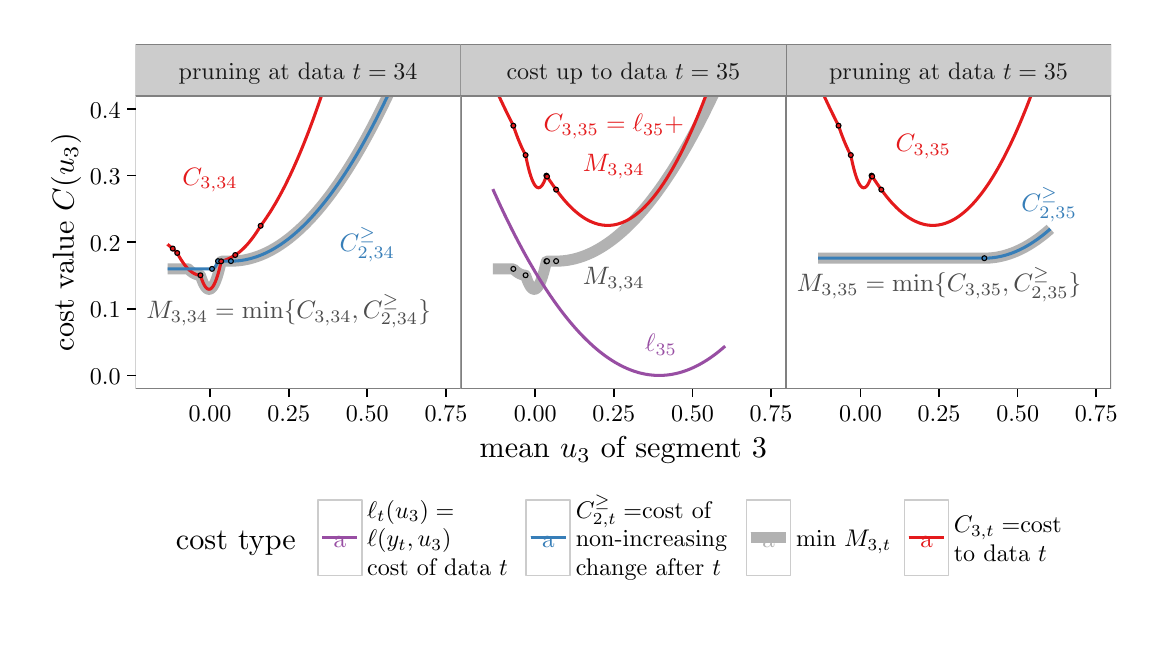
\begin{tikzpicture}[x=1pt,y=1pt]
\definecolor{fillColor}{RGB}{255,255,255}
\path[use as bounding box,fill=fillColor,fill opacity=0.00] (0,0) rectangle (397.48,216.81);
\begin{scope}
\path[clip] (  0.00,  0.00) rectangle (397.48,216.81);
\definecolor{drawColor}{RGB}{255,255,255}
\definecolor{fillColor}{RGB}{255,255,255}

\path[draw=drawColor,line width= 0.6pt,line join=round,line cap=round,fill=fillColor] (  0.00,  0.00) rectangle (397.48,216.81);
\end{scope}
\begin{scope}
\path[clip] ( 38.97,192.23) rectangle (156.48,210.81);
\definecolor{drawColor}{gray}{0.50}
\definecolor{fillColor}{gray}{0.80}

\path[draw=drawColor,line width= 0.2pt,line join=round,line cap=round,fill=fillColor] ( 38.97,192.23) rectangle (156.48,210.81);
\definecolor{drawColor}{gray}{0.10}

\node[text=drawColor,anchor=base,inner sep=0pt, outer sep=0pt, scale=  0.87] at ( 97.72,198.23) {pruning at data $t=34$};
\end{scope}
\begin{scope}
\path[clip] (156.48,192.23) rectangle (273.98,210.81);
\definecolor{drawColor}{gray}{0.50}
\definecolor{fillColor}{gray}{0.80}

\path[draw=drawColor,line width= 0.2pt,line join=round,line cap=round,fill=fillColor] (156.48,192.23) rectangle (273.98,210.81);
\definecolor{drawColor}{gray}{0.10}

\node[text=drawColor,anchor=base,inner sep=0pt, outer sep=0pt, scale=  0.87] at (215.23,198.23) {cost up to data $t=35$};
\end{scope}
\begin{scope}
\path[clip] (273.98,192.23) rectangle (391.48,210.81);
\definecolor{drawColor}{gray}{0.50}
\definecolor{fillColor}{gray}{0.80}

\path[draw=drawColor,line width= 0.2pt,line join=round,line cap=round,fill=fillColor] (273.98,192.23) rectangle (391.48,210.81);
\definecolor{drawColor}{gray}{0.10}

\node[text=drawColor,anchor=base,inner sep=0pt, outer sep=0pt, scale=  0.87] at (332.73,198.23) {pruning at data $t=35$};
\end{scope}
\begin{scope}
\path[clip] ( 38.97, 86.33) rectangle (156.48,192.23);
\definecolor{fillColor}{RGB}{255,255,255}

\path[fill=fillColor] ( 38.97, 86.33) rectangle (156.48,192.23);
\definecolor{drawColor}{gray}{0.70}

\path[draw=drawColor,line width= 4.0pt,line join=round] ( 50.58,129.65) --
	( 50.65,129.65) --
	( 50.73,129.65) --
	( 50.80,129.65) --
	( 50.88,129.65) --
	( 50.95,129.65) --
	( 51.02,129.65) --
	( 51.10,129.65) --
	( 51.17,129.65) --
	( 51.25,129.65) --
	( 51.32,129.65) --
	( 51.40,129.65) --
	( 51.47,129.65) --
	( 51.55,129.65) --
	( 51.62,129.65) --
	( 51.70,129.65) --
	( 51.77,129.65) --
	( 51.85,129.65) --
	( 51.92,129.65) --
	( 52.00,129.65) --
	( 52.07,129.65) --
	( 52.15,129.65) --
	( 52.22,129.65) --
	( 52.30,129.65) --
	( 52.37,129.65) --
	( 52.45,129.65) --
	( 52.52,129.65) --
	( 52.60,129.65) --
	( 52.67,129.65) --
	( 52.75,129.65) --
	( 52.82,129.65) --
	( 52.90,129.65) --
	( 52.97,129.65) --
	( 53.05,129.65) --
	( 53.12,129.65) --
	( 53.20,129.65) --
	( 53.27,129.65) --
	( 53.35,129.65) --
	( 53.42,129.65) --
	( 53.50,129.65) --
	( 53.57,129.65) --
	( 53.65,129.65) --
	( 53.72,129.65) --
	( 53.80,129.65) --
	( 53.87,129.65) --
	( 53.95,129.65) --
	( 54.02,129.65) --
	( 54.10,129.65) --
	( 54.17,129.65) --
	( 54.25,129.65) --
	( 54.32,129.65) --
	( 54.39,129.65) --
	( 54.47,129.65) --
	( 54.54,129.65) --
	( 54.62,129.65) --
	( 54.69,129.65) --
	( 54.77,129.65) --
	( 54.84,129.65) --
	( 54.92,129.65) --
	( 54.99,129.65) --
	( 55.07,129.65) --
	( 55.14,129.65) --
	( 55.22,129.65) --
	( 55.29,129.65) --
	( 55.37,129.65) --
	( 55.44,129.65) --
	( 55.52,129.65) --
	( 55.59,129.65) --
	( 55.67,129.65) --
	( 55.74,129.65) --
	( 55.82,129.65) --
	( 55.89,129.65) --
	( 55.97,129.65) --
	( 56.04,129.65) --
	( 56.12,129.65) --
	( 56.19,129.65) --
	( 56.27,129.65) --
	( 56.34,129.65) --
	( 56.42,129.65) --
	( 56.49,129.65) --
	( 56.57,129.65) --
	( 56.64,129.65) --
	( 56.72,129.65) --
	( 56.79,129.65) --
	( 56.87,129.65) --
	( 56.94,129.65) --
	( 57.02,129.65) --
	( 57.09,129.65) --
	( 57.17,129.65) --
	( 57.24,129.65) --
	( 57.32,129.65) --
	( 57.39,129.65) --
	( 57.47,129.65) --
	( 57.54,129.65) --
	( 57.61,129.65) --
	( 57.69,129.65) --
	( 57.76,129.65) --
	( 57.84,129.65) --
	( 57.91,129.65) --
	( 57.99,129.65) --
	( 57.99,129.65) --
	( 58.03,129.60) --
	( 58.08,129.56) --
	( 58.12,129.51) --
	( 58.17,129.47) --
	( 58.21,129.43) --
	( 58.26,129.38) --
	( 58.30,129.34) --
	( 58.35,129.30) --
	( 58.39,129.26) --
	( 58.44,129.21) --
	( 58.48,129.17) --
	( 58.53,129.13) --
	( 58.57,129.09) --
	( 58.62,129.05) --
	( 58.66,129.02) --
	( 58.71,128.98) --
	( 58.75,128.94) --
	( 58.79,128.90) --
	( 58.84,128.86) --
	( 58.88,128.83) --
	( 58.93,128.79) --
	( 58.97,128.76) --
	( 59.02,128.72) --
	( 59.06,128.69) --
	( 59.11,128.65) --
	( 59.15,128.62) --
	( 59.20,128.58) --
	( 59.24,128.55) --
	( 59.29,128.52) --
	( 59.33,128.49) --
	( 59.38,128.45) --
	( 59.42,128.42) --
	( 59.47,128.39) --
	( 59.51,128.36) --
	( 59.55,128.33) --
	( 59.60,128.30) --
	( 59.64,128.27) --
	( 59.69,128.24) --
	( 59.73,128.22) --
	( 59.78,128.19) --
	( 59.82,128.16) --
	( 59.87,128.13) --
	( 59.91,128.11) --
	( 59.96,128.08) --
	( 60.00,128.06) --
	( 60.05,128.03) --
	( 60.09,128.01) --
	( 60.14,127.98) --
	( 60.18,127.96) --
	( 60.23,127.94) --
	( 60.27,127.91) --
	( 60.32,127.89) --
	( 60.36,127.87) --
	( 60.40,127.85) --
	( 60.45,127.83) --
	( 60.49,127.81) --
	( 60.54,127.79) --
	( 60.58,127.77) --
	( 60.63,127.75) --
	( 60.67,127.73) --
	( 60.72,127.71) --
	( 60.76,127.69) --
	( 60.81,127.67) --
	( 60.85,127.66) --
	( 60.90,127.64) --
	( 60.94,127.62) --
	( 60.99,127.61) --
	( 61.03,127.59) --
	( 61.08,127.58) --
	( 61.12,127.57) --
	( 61.17,127.55) --
	( 61.21,127.54) --
	( 61.25,127.52) --
	( 61.30,127.51) --
	( 61.34,127.50) --
	( 61.39,127.49) --
	( 61.43,127.48) --
	( 61.48,127.47) --
	( 61.52,127.46) --
	( 61.57,127.45) --
	( 61.61,127.44) --
	( 61.66,127.43) --
	( 61.70,127.42) --
	( 61.75,127.41) --
	( 61.79,127.40) --
	( 61.84,127.40) --
	( 61.88,127.39) --
	( 61.93,127.38) --
	( 61.97,127.38) --
	( 62.02,127.37) --
	( 62.06,127.37) --
	( 62.10,127.36) --
	( 62.15,127.36) --
	( 62.19,127.36) --
	( 62.24,127.35) --
	( 62.28,127.35) --
	( 62.33,127.35) --
	( 62.37,127.35) --
	( 62.42,127.35) --
	( 62.42,127.35) --
	( 62.49,127.10) --
	( 62.57,126.86) --
	( 62.65,126.63) --
	( 62.72,126.41) --
	( 62.80,126.19) --
	( 62.87,125.97) --
	( 62.95,125.77) --
	( 63.03,125.56) --
	( 63.10,125.37) --
	( 63.18,125.18) --
	( 63.25,125.00) --
	( 63.33,124.82) --
	( 63.40,124.65) --
	( 63.48,124.48) --
	( 63.56,124.32) --
	( 63.63,124.17) --
	( 63.71,124.02) --
	( 63.78,123.88) --
	( 63.86,123.74) --
	( 63.94,123.61) --
	( 64.01,123.49) --
	( 64.09,123.37) --
	( 64.16,123.26) --
	( 64.24,123.16) --
	( 64.32,123.06) --
	( 64.39,122.96) --
	( 64.47,122.88) --
	( 64.54,122.80) --
	( 64.62,122.72) --
	( 64.69,122.65) --
	( 64.77,122.59) --
	( 64.85,122.53) --
	( 64.92,122.48) --
	( 65.00,122.43) --
	( 65.07,122.39) --
	( 65.15,122.36) --
	( 65.23,122.33) --
	( 65.30,122.31) --
	( 65.38,122.30) --
	( 65.45,122.29) --
	( 65.53,122.28) --
	( 65.61,122.29) --
	( 65.68,122.30) --
	( 65.76,122.31) --
	( 65.83,122.33) --
	( 65.91,122.36) --
	( 65.98,122.39) --
	( 66.06,122.43) --
	( 66.14,122.48) --
	( 66.21,122.53) --
	( 66.29,122.58) --
	( 66.36,122.65) --
	( 66.44,122.71) --
	( 66.52,122.79) --
	( 66.59,122.87) --
	( 66.67,122.96) --
	( 66.74,123.05) --
	( 66.82,123.15) --
	( 66.90,123.25) --
	( 66.97,123.37) --
	( 67.05,123.48) --
	( 67.12,123.61) --
	( 67.20,123.73) --
	( 67.28,123.87) --
	( 67.35,124.01) --
	( 67.43,124.16) --
	( 67.50,124.31) --
	( 67.58,124.47) --
	( 67.65,124.64) --
	( 67.73,124.81) --
	( 67.81,124.98) --
	( 67.88,125.17) --
	( 67.96,125.36) --
	( 68.03,125.55) --
	( 68.11,125.75) --
	( 68.19,125.96) --
	( 68.26,126.17) --
	( 68.34,126.39) --
	( 68.41,126.62) --
	( 68.49,126.85) --
	( 68.57,127.09) --
	( 68.64,127.33) --
	( 68.72,127.58) --
	( 68.79,127.83) --
	( 68.87,128.09) --
	( 68.94,128.36) --
	( 69.02,128.63) --
	( 69.10,128.91) --
	( 69.17,129.20) --
	( 69.25,129.49) --
	( 69.32,129.79) --
	( 69.40,130.09) --
	( 69.48,130.40) --
	( 69.55,130.72) --
	( 69.63,131.04) --
	( 69.70,131.36) --
	( 69.78,131.70) --
	( 69.86,132.04) --
	( 69.93,132.38) --
	( 69.93,132.38) --
	( 69.93,132.38) --
	( 69.94,132.38) --
	( 69.94,132.38) --
	( 69.94,132.39) --
	( 69.94,132.39) --
	( 69.95,132.39) --
	( 69.95,132.39) --
	( 69.95,132.39) --
	( 69.95,132.39) --
	( 69.96,132.39) --
	( 69.96,132.39) --
	( 69.96,132.39) --
	( 69.96,132.39) --
	( 69.96,132.39) --
	( 69.97,132.39) --
	( 69.97,132.39) --
	( 69.97,132.39) --
	( 69.97,132.39) --
	( 69.98,132.39) --
	( 69.98,132.40) --
	( 69.98,132.40) --
	( 69.98,132.40) --
	( 69.99,132.40) --
	( 69.99,132.40) --
	( 69.99,132.40) --
	( 69.99,132.40) --
	( 70.00,132.40) --
	( 70.00,132.40) --
	( 70.00,132.40) --
	( 70.00,132.40) --
	( 70.01,132.40) --
	( 70.01,132.40) --
	( 70.01,132.40) --
	( 70.01,132.40) --
	( 70.02,132.40) --
	( 70.02,132.41) --
	( 70.02,132.41) --
	( 70.02,132.41) --
	( 70.02,132.41) --
	( 70.03,132.41) --
	( 70.03,132.41) --
	( 70.03,132.41) --
	( 70.03,132.41) --
	( 70.04,132.41) --
	( 70.04,132.41) --
	( 70.04,132.41) --
	( 70.04,132.41) --
	( 70.05,132.41) --
	( 70.05,132.41) --
	( 70.05,132.41) --
	( 70.05,132.42) --
	( 70.06,132.42) --
	( 70.06,132.42) --
	( 70.06,132.42) --
	( 70.06,132.42) --
	( 70.07,132.42) --
	( 70.07,132.42) --
	( 70.07,132.42) --
	( 70.07,132.42) --
	( 70.08,132.42) --
	( 70.08,132.42) --
	( 70.08,132.42) --
	( 70.08,132.42) --
	( 70.08,132.42) --
	( 70.09,132.42) --
	( 70.09,132.42) --
	( 70.09,132.43) --
	( 70.09,132.43) --
	( 70.10,132.43) --
	( 70.10,132.43) --
	( 70.10,132.43) --
	( 70.10,132.43) --
	( 70.11,132.43) --
	( 70.11,132.43) --
	( 70.11,132.43) --
	( 70.11,132.43) --
	( 70.12,132.43) --
	( 70.12,132.43) --
	( 70.12,132.43) --
	( 70.12,132.43) --
	( 70.13,132.43) --
	( 70.13,132.44) --
	( 70.13,132.44) --
	( 70.13,132.44) --
	( 70.14,132.44) --
	( 70.14,132.44) --
	( 70.14,132.44) --
	( 70.14,132.44) --
	( 70.14,132.44) --
	( 70.15,132.44) --
	( 70.15,132.44) --
	( 70.15,132.44) --
	( 70.15,132.44) --
	( 70.16,132.44) --
	( 70.16,132.44) --
	( 70.16,132.44) --
	( 70.16,132.45) --
	( 70.17,132.45) --
	( 70.17,132.45) --
	( 70.17,132.45) --
	( 70.20,132.45) --
	( 70.24,132.45) --
	( 70.27,132.45) --
	( 70.30,132.45) --
	( 70.33,132.45) --
	( 70.37,132.45) --
	( 70.40,132.45) --
	( 70.43,132.45) --
	( 70.47,132.45) --
	( 70.50,132.45) --
	( 70.53,132.45) --
	( 70.57,132.45) --
	( 70.60,132.45) --
	( 70.63,132.45) --
	( 70.67,132.45) --
	( 70.70,132.45) --
	( 70.73,132.45) --
	( 70.77,132.45) --
	( 70.80,132.45) --
	( 70.83,132.45) --
	( 70.87,132.45) --
	( 70.90,132.45) --
	( 70.93,132.45) --
	( 70.96,132.45) --
	( 71.00,132.45) --
	( 71.03,132.45) --
	( 71.06,132.45) --
	( 71.10,132.45) --
	( 71.13,132.45) --
	( 71.16,132.45) --
	( 71.20,132.45) --
	( 71.23,132.45) --
	( 71.26,132.45) --
	( 71.30,132.45) --
	( 71.33,132.45) --
	( 71.36,132.45) --
	( 71.40,132.45) --
	( 71.43,132.45) --
	( 71.46,132.45) --
	( 71.50,132.45) --
	( 71.53,132.45) --
	( 71.56,132.45) --
	( 71.59,132.45) --
	( 71.63,132.45) --
	( 71.66,132.45) --
	( 71.69,132.45) --
	( 71.73,132.45) --
	( 71.76,132.45) --
	( 71.79,132.45) --
	( 71.83,132.45) --
	( 71.86,132.45) --
	( 71.89,132.45) --
	( 71.93,132.45) --
	( 71.96,132.45) --
	( 71.99,132.45) --
	( 72.03,132.45) --
	( 72.06,132.45) --
	( 72.09,132.45) --
	( 72.13,132.45) --
	( 72.16,132.45) --
	( 72.19,132.45) --
	( 72.23,132.45) --
	( 72.26,132.45) --
	( 72.29,132.45) --
	( 72.32,132.45) --
	( 72.36,132.45) --
	( 72.39,132.45) --
	( 72.42,132.45) --
	( 72.46,132.45) --
	( 72.49,132.45) --
	( 72.52,132.45) --
	( 72.56,132.45) --
	( 72.59,132.45) --
	( 72.62,132.45) --
	( 72.66,132.45) --
	( 72.69,132.45) --
	( 72.72,132.45) --
	( 72.76,132.45) --
	( 72.79,132.45) --
	( 72.82,132.45) --
	( 72.86,132.45) --
	( 72.89,132.45) --
	( 72.92,132.45) --
	( 72.95,132.45) --
	( 72.99,132.45) --
	( 73.02,132.45) --
	( 73.05,132.45) --
	( 73.09,132.45) --
	( 73.12,132.45) --
	( 73.15,132.45) --
	( 73.19,132.45) --
	( 73.22,132.45) --
	( 73.25,132.45) --
	( 73.29,132.45) --
	( 73.32,132.45) --
	( 73.35,132.45) --
	( 73.39,132.45) --
	( 73.42,132.45) --
	( 73.45,132.45) --
	( 73.45,132.45) --
	( 74.07,132.45) --
	( 74.69,132.47) --
	( 75.30,132.51) --
	( 75.92,132.56) --
	( 76.54,132.62) --
	( 77.15,132.70) --
	( 77.77,132.79) --
	( 78.39,132.90) --
	( 79.00,133.02) --
	( 79.62,133.16) --
	( 80.24,133.30) --
	( 80.85,133.47) --
	( 81.47,133.65) --
	( 82.09,133.84) --
	( 82.71,134.04) --
	( 83.32,134.26) --
	( 83.94,134.50) --
	( 84.56,134.74) --
	( 85.17,135.01) --
	( 85.79,135.28) --
	( 86.41,135.57) --
	( 87.02,135.88) --
	( 87.64,136.20) --
	( 88.26,136.53) --
	( 88.87,136.88) --
	( 89.49,137.24) --
	( 90.11,137.62) --
	( 90.73,138.01) --
	( 91.34,138.41) --
	( 91.96,138.83) --
	( 92.58,139.26) --
	( 93.19,139.71) --
	( 93.81,140.17) --
	( 94.43,140.64) --
	( 95.04,141.13) --
	( 95.66,141.64) --
	( 96.28,142.16) --
	( 96.89,142.69) --
	( 97.51,143.23) --
	( 98.13,143.79) --
	( 98.74,144.37) --
	( 99.36,144.96) --
	( 99.98,145.56) --
	(100.60,146.18) --
	(101.21,146.81) --
	(101.83,147.45) --
	(102.45,148.11) --
	(103.06,148.79) --
	(103.68,149.47) --
	(104.30,150.18) --
	(104.91,150.89) --
	(105.53,151.62) --
	(106.15,152.37) --
	(106.76,153.13) --
	(107.38,153.90) --
	(108.00,154.69) --
	(108.62,155.49) --
	(109.23,156.30) --
	(109.85,157.13) --
	(110.47,157.98) --
	(111.08,158.84) --
	(111.70,159.71) --
	(112.32,160.59) --
	(112.93,161.50) --
	(113.55,162.41) --
	(114.17,163.34) --
	(114.78,164.28) --
	(115.40,165.24) --
	(116.02,166.21) --
	(116.63,167.20) --
	(117.25,168.20) --
	(117.87,169.21) --
	(118.49,170.24) --
	(119.10,171.28) --
	(119.72,172.34) --
	(120.34,173.41) --
	(120.95,174.49) --
	(121.57,175.59) --
	(122.19,176.71) --
	(122.80,177.84) --
	(123.42,178.98) --
	(124.04,180.13) --
	(124.65,181.30) --
	(125.27,182.49) --
	(125.89,183.69) --
	(126.50,184.90) --
	(127.12,186.13) --
	(127.74,187.37) --
	(128.36,188.62) --
	(128.97,189.89) --
	(129.59,191.18) --
	(130.21,192.47) --
	(130.82,193.79) --
	(131.44,195.11) --
	(132.06,196.45) --
	(132.67,197.81) --
	(133.29,199.17) --
	(133.91,200.56) --
	(134.52,201.95);
\definecolor{drawColor}{RGB}{228,26,28}

\path[draw=drawColor,line width= 1.1pt,line join=round] ( 50.58,138.50) --
	( 50.59,138.48) --
	( 50.61,138.47) --
	( 50.63,138.45) --
	( 50.65,138.44) --
	( 50.67,138.42) --
	( 50.69,138.41) --
	( 50.71,138.39) --
	( 50.73,138.37) --
	( 50.74,138.36) --
	( 50.76,138.34) --
	( 50.78,138.33) --
	( 50.80,138.31) --
	( 50.82,138.29) --
	( 50.84,138.28) --
	( 50.86,138.26) --
	( 50.88,138.25) --
	( 50.89,138.23) --
	( 50.91,138.21) --
	( 50.93,138.20) --
	( 50.95,138.18) --
	( 50.97,138.17) --
	( 50.99,138.15) --
	( 51.01,138.14) --
	( 51.03,138.12) --
	( 51.04,138.10) --
	( 51.06,138.09) --
	( 51.08,138.07) --
	( 51.10,138.06) --
	( 51.12,138.04) --
	( 51.14,138.03) --
	( 51.16,138.01) --
	( 51.18,138.00) --
	( 51.20,137.98) --
	( 51.21,137.96) --
	( 51.23,137.95) --
	( 51.25,137.93) --
	( 51.27,137.92) --
	( 51.29,137.90) --
	( 51.31,137.89) --
	( 51.33,137.87) --
	( 51.35,137.86) --
	( 51.36,137.84) --
	( 51.38,137.82) --
	( 51.40,137.81) --
	( 51.42,137.79) --
	( 51.44,137.78) --
	( 51.46,137.76) --
	( 51.48,137.75) --
	( 51.50,137.73) --
	( 51.51,137.72) --
	( 51.53,137.70) --
	( 51.55,137.69) --
	( 51.57,137.67) --
	( 51.59,137.66) --
	( 51.61,137.64) --
	( 51.63,137.63) --
	( 51.65,137.61) --
	( 51.66,137.59) --
	( 51.68,137.58) --
	( 51.70,137.56) --
	( 51.72,137.55) --
	( 51.74,137.53) --
	( 51.76,137.52) --
	( 51.78,137.50) --
	( 51.80,137.49) --
	( 51.81,137.47) --
	( 51.83,137.46) --
	( 51.85,137.44) --
	( 51.87,137.43) --
	( 51.89,137.41) --
	( 51.91,137.40) --
	( 51.93,137.38) --
	( 51.95,137.37) --
	( 51.96,137.35) --
	( 51.98,137.34) --
	( 52.00,137.32) --
	( 52.02,137.31) --
	( 52.04,137.29) --
	( 52.06,137.28) --
	( 52.08,137.26) --
	( 52.10,137.25) --
	( 52.12,137.23) --
	( 52.13,137.22) --
	( 52.15,137.20) --
	( 52.17,137.19) --
	( 52.19,137.17) --
	( 52.21,137.16) --
	( 52.23,137.14) --
	( 52.25,137.13) --
	( 52.27,137.11) --
	( 52.28,137.10) --
	( 52.30,137.08) --
	( 52.32,137.07) --
	( 52.34,137.05) --
	( 52.36,137.04) --
	( 52.38,137.02) --
	( 52.40,137.01) --
	( 52.42,137.00) --
	( 52.43,136.98) --
	( 52.43,136.98) --
	( 52.45,136.96) --
	( 52.47,136.95) --
	( 52.48,136.93) --
	( 52.50,136.91) --
	( 52.52,136.90) --
	( 52.53,136.88) --
	( 52.55,136.86) --
	( 52.56,136.85) --
	( 52.58,136.83) --
	( 52.60,136.81) --
	( 52.61,136.80) --
	( 52.63,136.78) --
	( 52.65,136.76) --
	( 52.66,136.74) --
	( 52.68,136.73) --
	( 52.69,136.71) --
	( 52.71,136.69) --
	( 52.73,136.68) --
	( 52.74,136.66) --
	( 52.76,136.65) --
	( 52.78,136.63) --
	( 52.79,136.61) --
	( 52.81,136.60) --
	( 52.82,136.58) --
	( 52.84,136.56) --
	( 52.86,136.55) --
	( 52.87,136.53) --
	( 52.89,136.51) --
	( 52.90,136.50) --
	( 52.92,136.48) --
	( 52.94,136.46) --
	( 52.95,136.45) --
	( 52.97,136.43) --
	( 52.99,136.41) --
	( 53.00,136.40) --
	( 53.02,136.38) --
	( 53.03,136.37) --
	( 53.05,136.35) --
	( 53.07,136.33) --
	( 53.08,136.32) --
	( 53.10,136.30) --
	( 53.12,136.28) --
	( 53.13,136.27) --
	( 53.15,136.25) --
	( 53.16,136.24) --
	( 53.18,136.22) --
	( 53.20,136.20) --
	( 53.21,136.19) --
	( 53.23,136.17) --
	( 53.25,136.16) --
	( 53.26,136.14) --
	( 53.28,136.12) --
	( 53.29,136.11) --
	( 53.31,136.09) --
	( 53.33,136.08) --
	( 53.34,136.06) --
	( 53.36,136.04) --
	( 53.38,136.03) --
	( 53.39,136.01) --
	( 53.41,136.00) --
	( 53.42,135.98) --
	( 53.44,135.97) --
	( 53.46,135.95) --
	( 53.47,135.93) --
	( 53.49,135.92) --
	( 53.51,135.90) --
	( 53.52,135.89) --
	( 53.54,135.87) --
	( 53.55,135.86) --
	( 53.57,135.84) --
	( 53.59,135.82) --
	( 53.60,135.81) --
	( 53.62,135.79) --
	( 53.64,135.78) --
	( 53.65,135.76) --
	( 53.67,135.75) --
	( 53.68,135.73) --
	( 53.70,135.72) --
	( 53.72,135.70) --
	( 53.73,135.69) --
	( 53.75,135.67) --
	( 53.77,135.65) --
	( 53.78,135.64) --
	( 53.80,135.62) --
	( 53.81,135.61) --
	( 53.83,135.59) --
	( 53.85,135.58) --
	( 53.86,135.56) --
	( 53.88,135.55) --
	( 53.90,135.53) --
	( 53.91,135.52) --
	( 53.93,135.50) --
	( 53.94,135.49) --
	( 53.96,135.47) --
	( 53.98,135.46) --
	( 53.99,135.44) --
	( 54.01,135.43) --
	( 54.02,135.41) --
	( 54.04,135.40) --
	( 54.04,135.40) --
	( 54.13,135.24) --
	( 54.21,135.08) --
	( 54.30,134.92) --
	( 54.38,134.77) --
	( 54.46,134.61) --
	( 54.55,134.46) --
	( 54.63,134.31) --
	( 54.72,134.16) --
	( 54.80,134.02) --
	( 54.89,133.87) --
	( 54.97,133.73) --
	( 55.06,133.58) --
	( 55.14,133.44) --
	( 55.23,133.31) --
	( 55.31,133.17) --
	( 55.39,133.03) --
	( 55.48,132.90) --
	( 55.56,132.77) --
	( 55.65,132.63) --
	( 55.73,132.50) --
	( 55.82,132.38) --
	( 55.90,132.25) --
	( 55.99,132.13) --
	( 56.07,132.00) --
	( 56.16,131.88) --
	( 56.24,131.76) --
	( 56.33,131.64) --
	( 56.41,131.53) --
	( 56.49,131.41) --
	( 56.58,131.30) --
	( 56.66,131.19) --
	( 56.75,131.08) --
	( 56.83,130.97) --
	( 56.92,130.86) --
	( 57.00,130.76) --
	( 57.09,130.65) --
	( 57.17,130.55) --
	( 57.26,130.45) --
	( 57.34,130.35) --
	( 57.43,130.25) --
	( 57.51,130.16) --
	( 57.59,130.06) --
	( 57.68,129.97) --
	( 57.76,129.88) --
	( 57.85,129.79) --
	( 57.93,129.70) --
	( 58.02,129.62) --
	( 58.10,129.53) --
	( 58.19,129.45) --
	( 58.27,129.37) --
	( 58.36,129.29) --
	( 58.44,129.21) --
	( 58.53,129.13) --
	( 58.61,129.06) --
	( 58.69,128.99) --
	( 58.78,128.91) --
	( 58.86,128.84) --
	( 58.95,128.78) --
	( 59.03,128.71) --
	( 59.12,128.64) --
	( 59.20,128.58) --
	( 59.29,128.52) --
	( 59.37,128.46) --
	( 59.46,128.40) --
	( 59.54,128.34) --
	( 59.63,128.29) --
	( 59.71,128.23) --
	( 59.79,128.18) --
	( 59.88,128.13) --
	( 59.96,128.08) --
	( 60.05,128.03) --
	( 60.13,127.98) --
	( 60.22,127.94) --
	( 60.30,127.90) --
	( 60.39,127.86) --
	( 60.47,127.82) --
	( 60.56,127.78) --
	( 60.64,127.74) --
	( 60.73,127.71) --
	( 60.81,127.67) --
	( 60.89,127.64) --
	( 60.98,127.61) --
	( 61.06,127.58) --
	( 61.15,127.56) --
	( 61.23,127.53) --
	( 61.32,127.51) --
	( 61.40,127.49) --
	( 61.49,127.46) --
	( 61.57,127.45) --
	( 61.66,127.43) --
	( 61.74,127.41) --
	( 61.83,127.40) --
	( 61.91,127.39) --
	( 61.99,127.38) --
	( 62.08,127.37) --
	( 62.16,127.36) --
	( 62.25,127.35) --
	( 62.33,127.35) --
	( 62.42,127.35) --
	( 62.42,127.35) --
	( 62.49,127.10) --
	( 62.57,126.86) --
	( 62.65,126.63) --
	( 62.72,126.41) --
	( 62.80,126.19) --
	( 62.87,125.97) --
	( 62.95,125.77) --
	( 63.03,125.56) --
	( 63.10,125.37) --
	( 63.18,125.18) --
	( 63.25,125.00) --
	( 63.33,124.82) --
	( 63.40,124.65) --
	( 63.48,124.48) --
	( 63.56,124.32) --
	( 63.63,124.17) --
	( 63.71,124.02) --
	( 63.78,123.88) --
	( 63.86,123.74) --
	( 63.94,123.61) --
	( 64.01,123.49) --
	( 64.09,123.37) --
	( 64.16,123.26) --
	( 64.24,123.16) --
	( 64.32,123.06) --
	( 64.39,122.96) --
	( 64.47,122.88) --
	( 64.54,122.80) --
	( 64.62,122.72) --
	( 64.69,122.65) --
	( 64.77,122.59) --
	( 64.85,122.53) --
	( 64.92,122.48) --
	( 65.00,122.43) --
	( 65.07,122.39) --
	( 65.15,122.36) --
	( 65.23,122.33) --
	( 65.30,122.31) --
	( 65.38,122.30) --
	( 65.45,122.29) --
	( 65.53,122.28) --
	( 65.61,122.29) --
	( 65.68,122.30) --
	( 65.76,122.31) --
	( 65.83,122.33) --
	( 65.91,122.36) --
	( 65.98,122.39) --
	( 66.06,122.43) --
	( 66.14,122.48) --
	( 66.21,122.53) --
	( 66.29,122.58) --
	( 66.36,122.65) --
	( 66.44,122.71) --
	( 66.52,122.79) --
	( 66.59,122.87) --
	( 66.67,122.96) --
	( 66.74,123.05) --
	( 66.82,123.15) --
	( 66.90,123.25) --
	( 66.97,123.37) --
	( 67.05,123.48) --
	( 67.12,123.61) --
	( 67.20,123.73) --
	( 67.28,123.87) --
	( 67.35,124.01) --
	( 67.43,124.16) --
	( 67.50,124.31) --
	( 67.58,124.47) --
	( 67.65,124.64) --
	( 67.73,124.81) --
	( 67.81,124.98) --
	( 67.88,125.17) --
	( 67.96,125.36) --
	( 68.03,125.55) --
	( 68.11,125.75) --
	( 68.19,125.96) --
	( 68.26,126.17) --
	( 68.34,126.39) --
	( 68.41,126.62) --
	( 68.49,126.85) --
	( 68.57,127.09) --
	( 68.64,127.33) --
	( 68.72,127.58) --
	( 68.79,127.83) --
	( 68.87,128.09) --
	( 68.94,128.36) --
	( 69.02,128.63) --
	( 69.10,128.91) --
	( 69.17,129.20) --
	( 69.25,129.49) --
	( 69.32,129.79) --
	( 69.40,130.09) --
	( 69.48,130.40) --
	( 69.55,130.72) --
	( 69.63,131.04) --
	( 69.70,131.36) --
	( 69.78,131.70) --
	( 69.86,132.04) --
	( 69.93,132.38) --
	( 69.93,132.38) --
	( 69.98,132.40) --
	( 70.03,132.41) --
	( 70.09,132.42) --
	( 70.14,132.44) --
	( 70.19,132.45) --
	( 70.24,132.47) --
	( 70.29,132.48) --
	( 70.34,132.50) --
	( 70.39,132.51) --
	( 70.44,132.53) --
	( 70.49,132.54) --
	( 70.55,132.56) --
	( 70.60,132.57) --
	( 70.65,132.59) --
	( 70.70,132.60) --
	( 70.75,132.62) --
	( 70.80,132.64) --
	( 70.85,132.65) --
	( 70.90,132.67) --
	( 70.96,132.69) --
	( 71.01,132.70) --
	( 71.06,132.72) --
	( 71.11,132.74) --
	( 71.16,132.76) --
	( 71.21,132.78) --
	( 71.26,132.79) --
	( 71.31,132.81) --
	( 71.37,132.83) --
	( 71.42,132.85) --
	( 71.47,132.87) --
	( 71.52,132.89) --
	( 71.57,132.91) --
	( 71.62,132.93) --
	( 71.67,132.95) --
	( 71.72,132.97) --
	( 71.78,132.99) --
	( 71.83,133.01) --
	( 71.88,133.03) --
	( 71.93,133.05) --
	( 71.98,133.07) --
	( 72.03,133.09) --
	( 72.08,133.11) --
	( 72.13,133.13) --
	( 72.19,133.16) --
	( 72.24,133.18) --
	( 72.29,133.20) --
	( 72.34,133.22) --
	( 72.39,133.24) --
	( 72.44,133.27) --
	( 72.49,133.29) --
	( 72.54,133.31) --
	( 72.60,133.34) --
	( 72.65,133.36) --
	( 72.70,133.38) --
	( 72.75,133.41) --
	( 72.80,133.43) --
	( 72.85,133.46) --
	( 72.90,133.48) --
	( 72.95,133.51) --
	( 73.01,133.53) --
	( 73.06,133.56) --
	( 73.11,133.58) --
	( 73.16,133.61) --
	( 73.21,133.63) --
	( 73.26,133.66) --
	( 73.31,133.68) --
	( 73.36,133.71) --
	( 73.42,133.74) --
	( 73.47,133.76) --
	( 73.52,133.79) --
	( 73.57,133.82) --
	( 73.62,133.84) --
	( 73.67,133.87) --
	( 73.72,133.90) --
	( 73.77,133.93) --
	( 73.83,133.96) --
	( 73.88,133.98) --
	( 73.93,134.01) --
	( 73.98,134.04) --
	( 74.03,134.07) --
	( 74.08,134.10) --
	( 74.13,134.13) --
	( 74.18,134.16) --
	( 74.24,134.19) --
	( 74.29,134.22) --
	( 74.34,134.25) --
	( 74.39,134.28) --
	( 74.44,134.31) --
	( 74.49,134.34) --
	( 74.54,134.37) --
	( 74.59,134.40) --
	( 74.65,134.43) --
	( 74.70,134.46) --
	( 74.75,134.49) --
	( 74.80,134.53) --
	( 74.85,134.56) --
	( 74.90,134.59) --
	( 74.95,134.62) --
	( 75.00,134.65) --
	( 75.00,134.65) --
	( 75.10,134.71) --
	( 75.19,134.77) --
	( 75.28,134.84) --
	( 75.38,134.90) --
	( 75.47,134.96) --
	( 75.56,135.03) --
	( 75.65,135.09) --
	( 75.75,135.16) --
	( 75.84,135.22) --
	( 75.93,135.29) --
	( 76.02,135.36) --
	( 76.12,135.43) --
	( 76.21,135.50) --
	( 76.30,135.57) --
	( 76.40,135.65) --
	( 76.49,135.72) --
	( 76.58,135.80) --
	( 76.67,135.87) --
	( 76.77,135.95) --
	( 76.86,136.03) --
	( 76.95,136.11) --
	( 77.04,136.19) --
	( 77.14,136.27) --
	( 77.23,136.35) --
	( 77.32,136.43) --
	( 77.41,136.51) --
	( 77.51,136.60) --
	( 77.60,136.68) --
	( 77.69,136.77) --
	( 77.79,136.86) --
	( 77.88,136.95) --
	( 77.97,137.04) --
	( 78.06,137.13) --
	( 78.16,137.22) --
	( 78.25,137.31) --
	( 78.34,137.40) --
	( 78.43,137.50) --
	( 78.53,137.59) --
	( 78.62,137.69) --
	( 78.71,137.78) --
	( 78.81,137.88) --
	( 78.90,137.98) --
	( 78.99,138.08) --
	( 79.08,138.18) --
	( 79.18,138.28) --
	( 79.27,138.39) --
	( 79.36,138.49) --
	( 79.45,138.59) --
	( 79.55,138.70) --
	( 79.64,138.81) --
	( 79.73,138.91) --
	( 79.83,139.02) --
	( 79.92,139.13) --
	( 80.01,139.24) --
	( 80.10,139.35) --
	( 80.20,139.47) --
	( 80.29,139.58) --
	( 80.38,139.69) --
	( 80.47,139.81) --
	( 80.57,139.93) --
	( 80.66,140.04) --
	( 80.75,140.16) --
	( 80.84,140.28) --
	( 80.94,140.40) --
	( 81.03,140.52) --
	( 81.12,140.64) --
	( 81.22,140.77) --
	( 81.31,140.89) --
	( 81.40,141.01) --
	( 81.49,141.14) --
	( 81.59,141.27) --
	( 81.68,141.39) --
	( 81.77,141.52) --
	( 81.86,141.65) --
	( 81.96,141.78) --
	( 82.05,141.92) --
	( 82.14,142.05) --
	( 82.24,142.18) --
	( 82.33,142.32) --
	( 82.42,142.45) --
	( 82.51,142.59) --
	( 82.61,142.72) --
	( 82.70,142.86) --
	( 82.79,143.00) --
	( 82.88,143.14) --
	( 82.98,143.28) --
	( 83.07,143.43) --
	( 83.16,143.57) --
	( 83.26,143.71) --
	( 83.35,143.86) --
	( 83.44,144.00) --
	( 83.53,144.15) --
	( 83.63,144.30) --
	( 83.72,144.45) --
	( 83.81,144.60) --
	( 83.90,144.75) --
	( 84.00,144.90) --
	( 84.09,145.05) --
	( 84.18,145.21) --
	( 84.18,145.21) --
	( 84.69,145.89) --
	( 85.20,146.59) --
	( 85.71,147.31) --
	( 86.22,148.05) --
	( 86.72,148.81) --
	( 87.23,149.58) --
	( 87.74,150.38) --
	( 88.25,151.20) --
	( 88.76,152.03) --
	( 89.27,152.89) --
	( 89.78,153.76) --
	( 90.28,154.65) --
	( 90.79,155.57) --
	( 91.30,156.50) --
	( 91.81,157.45) --
	( 92.32,158.42) --
	( 92.83,159.41) --
	( 93.34,160.42) --
	( 93.84,161.45) --
	( 94.35,162.50) --
	( 94.86,163.56) --
	( 95.37,164.65) --
	( 95.88,165.75) --
	( 96.39,166.88) --
	( 96.89,168.02) --
	( 97.40,169.19) --
	( 97.91,170.37) --
	( 98.42,171.57) --
	( 98.93,172.79) --
	( 99.44,174.03) --
	( 99.95,175.29) --
	(100.45,176.57) --
	(100.96,177.87) --
	(101.47,179.18) --
	(101.98,180.52) --
	(102.49,181.88) --
	(103.00,183.25) --
	(103.51,184.65) --
	(104.01,186.06) --
	(104.52,187.49) --
	(105.03,188.95) --
	(105.54,190.42) --
	(106.05,191.91) --
	(106.56,193.42) --
	(107.07,194.95) --
	(107.57,196.50) --
	(108.08,198.07) --
	(108.59,199.65) --
	(109.10,201.26) --
	(109.61,202.88) --
	(110.12,204.53) --
	(110.62,206.19) --
	(111.13,207.88) --
	(111.64,209.58) --
	(112.15,211.30) --
	(112.66,213.04) --
	(113.17,214.81) --
	(113.68,216.59) --
	(113.74,216.81);
\definecolor{drawColor}{RGB}{55,126,184}

\path[draw=drawColor,line width= 1.1pt,line join=round] ( 50.58,129.65) --
	( 50.74,129.65) --
	( 50.90,129.65) --
	( 51.06,129.65) --
	( 51.22,129.65) --
	( 51.39,129.65) --
	( 51.55,129.65) --
	( 51.71,129.65) --
	( 51.87,129.65) --
	( 52.03,129.65) --
	( 52.20,129.65) --
	( 52.36,129.65) --
	( 52.52,129.65) --
	( 52.68,129.65) --
	( 52.84,129.65) --
	( 53.01,129.65) --
	( 53.17,129.65) --
	( 53.33,129.65) --
	( 53.49,129.65) --
	( 53.65,129.65) --
	( 53.82,129.65) --
	( 53.98,129.65) --
	( 54.14,129.65) --
	( 54.30,129.65) --
	( 54.46,129.65) --
	( 54.63,129.65) --
	( 54.79,129.65) --
	( 54.95,129.65) --
	( 55.11,129.65) --
	( 55.27,129.65) --
	( 55.44,129.65) --
	( 55.60,129.65) --
	( 55.76,129.65) --
	( 55.92,129.65) --
	( 56.09,129.65) --
	( 56.25,129.65) --
	( 56.41,129.65) --
	( 56.57,129.65) --
	( 56.73,129.65) --
	( 56.90,129.65) --
	( 57.06,129.65) --
	( 57.22,129.65) --
	( 57.38,129.65) --
	( 57.54,129.65) --
	( 57.71,129.65) --
	( 57.87,129.65) --
	( 58.03,129.65) --
	( 58.19,129.65) --
	( 58.35,129.65) --
	( 58.52,129.65) --
	( 58.68,129.65) --
	( 58.84,129.65) --
	( 59.00,129.65) --
	( 59.16,129.65) --
	( 59.33,129.65) --
	( 59.49,129.65) --
	( 59.65,129.65) --
	( 59.81,129.65) --
	( 59.97,129.65) --
	( 60.14,129.65) --
	( 60.30,129.65) --
	( 60.46,129.65) --
	( 60.62,129.65) --
	( 60.78,129.65) --
	( 60.95,129.65) --
	( 61.11,129.65) --
	( 61.27,129.65) --
	( 61.43,129.65) --
	( 61.59,129.65) --
	( 61.76,129.65) --
	( 61.92,129.65) --
	( 62.08,129.65) --
	( 62.24,129.65) --
	( 62.40,129.65) --
	( 62.57,129.65) --
	( 62.73,129.65) --
	( 62.89,129.65) --
	( 63.05,129.65) --
	( 63.22,129.65) --
	( 63.38,129.65) --
	( 63.54,129.65) --
	( 63.70,129.65) --
	( 63.86,129.65) --
	( 64.03,129.65) --
	( 64.19,129.65) --
	( 64.35,129.65) --
	( 64.51,129.65) --
	( 64.67,129.65) --
	( 64.84,129.65) --
	( 65.00,129.65) --
	( 65.16,129.65) --
	( 65.32,129.65) --
	( 65.48,129.65) --
	( 65.65,129.65) --
	( 65.81,129.65) --
	( 65.97,129.65) --
	( 66.13,129.65) --
	( 66.29,129.65) --
	( 66.46,129.65) --
	( 66.62,129.65) --
	( 66.62,129.65) --
	( 66.64,129.65) --
	( 66.66,129.65) --
	( 66.68,129.65) --
	( 66.71,129.65) --
	( 66.73,129.65) --
	( 66.75,129.66) --
	( 66.77,129.66) --
	( 66.79,129.66) --
	( 66.82,129.67) --
	( 66.84,129.68) --
	( 66.86,129.68) --
	( 66.88,129.69) --
	( 66.90,129.69) --
	( 66.92,129.70) --
	( 66.95,129.71) --
	( 66.97,129.72) --
	( 66.99,129.73) --
	( 67.01,129.74) --
	( 67.03,129.75) --
	( 67.06,129.76) --
	( 67.08,129.77) --
	( 67.10,129.78) --
	( 67.12,129.80) --
	( 67.14,129.81) --
	( 67.17,129.83) --
	( 67.19,129.84) --
	( 67.21,129.85) --
	( 67.23,129.87) --
	( 67.25,129.89) --
	( 67.27,129.90) --
	( 67.30,129.92) --
	( 67.32,129.94) --
	( 67.34,129.96) --
	( 67.36,129.98) --
	( 67.38,130.00) --
	( 67.41,130.02) --
	( 67.43,130.04) --
	( 67.45,130.06) --
	( 67.47,130.08) --
	( 67.49,130.10) --
	( 67.52,130.13) --
	( 67.54,130.15) --
	( 67.56,130.17) --
	( 67.58,130.20) --
	( 67.60,130.23) --
	( 67.62,130.25) --
	( 67.65,130.28) --
	( 67.67,130.30) --
	( 67.69,130.33) --
	( 67.71,130.36) --
	( 67.73,130.39) --
	( 67.76,130.42) --
	( 67.78,130.45) --
	( 67.80,130.48) --
	( 67.82,130.51) --
	( 67.84,130.54) --
	( 67.87,130.57) --
	( 67.89,130.61) --
	( 67.91,130.64) --
	( 67.93,130.67) --
	( 67.95,130.71) --
	( 67.98,130.74) --
	( 68.00,130.78) --
	( 68.02,130.82) --
	( 68.04,130.85) --
	( 68.06,130.89) --
	( 68.08,130.93) --
	( 68.11,130.97) --
	( 68.13,131.01) --
	( 68.15,131.05) --
	( 68.17,131.09) --
	( 68.19,131.13) --
	( 68.22,131.17) --
	( 68.24,131.21) --
	( 68.26,131.25) --
	( 68.28,131.30) --
	( 68.30,131.34) --
	( 68.33,131.38) --
	( 68.35,131.43) --
	( 68.37,131.47) --
	( 68.39,131.52) --
	( 68.41,131.57) --
	( 68.43,131.61) --
	( 68.46,131.66) --
	( 68.48,131.71) --
	( 68.50,131.76) --
	( 68.52,131.81) --
	( 68.54,131.86) --
	( 68.57,131.91) --
	( 68.59,131.96) --
	( 68.61,132.01) --
	( 68.63,132.06) --
	( 68.65,132.12) --
	( 68.68,132.17) --
	( 68.70,132.22) --
	( 68.72,132.28) --
	( 68.74,132.33) --
	( 68.76,132.39) --
	( 68.78,132.45) --
	( 68.78,132.45) --
	( 68.83,132.45) --
	( 68.88,132.45) --
	( 68.93,132.45) --
	( 68.97,132.45) --
	( 69.02,132.45) --
	( 69.07,132.45) --
	( 69.11,132.45) --
	( 69.16,132.45) --
	( 69.21,132.45) --
	( 69.26,132.45) --
	( 69.30,132.45) --
	( 69.35,132.45) --
	( 69.40,132.45) --
	( 69.44,132.45) --
	( 69.49,132.45) --
	( 69.54,132.45) --
	( 69.59,132.45) --
	( 69.63,132.45) --
	( 69.68,132.45) --
	( 69.73,132.45) --
	( 69.77,132.45) --
	( 69.82,132.45) --
	( 69.87,132.45) --
	( 69.92,132.45) --
	( 69.96,132.45) --
	( 70.01,132.45) --
	( 70.06,132.45) --
	( 70.10,132.45) --
	( 70.15,132.45) --
	( 70.20,132.45) --
	( 70.25,132.45) --
	( 70.29,132.45) --
	( 70.34,132.45) --
	( 70.39,132.45) --
	( 70.43,132.45) --
	( 70.48,132.45) --
	( 70.53,132.45) --
	( 70.58,132.45) --
	( 70.62,132.45) --
	( 70.67,132.45) --
	( 70.72,132.45) --
	( 70.76,132.45) --
	( 70.81,132.45) --
	( 70.86,132.45) --
	( 70.91,132.45) --
	( 70.95,132.45) --
	( 71.00,132.45) --
	( 71.05,132.45) --
	( 71.10,132.45) --
	( 71.14,132.45) --
	( 71.19,132.45) --
	( 71.24,132.45) --
	( 71.28,132.45) --
	( 71.33,132.45) --
	( 71.38,132.45) --
	( 71.43,132.45) --
	( 71.47,132.45) --
	( 71.52,132.45) --
	( 71.57,132.45) --
	( 71.61,132.45) --
	( 71.66,132.45) --
	( 71.71,132.45) --
	( 71.76,132.45) --
	( 71.80,132.45) --
	( 71.85,132.45) --
	( 71.90,132.45) --
	( 71.94,132.45) --
	( 71.99,132.45) --
	( 72.04,132.45) --
	( 72.09,132.45) --
	( 72.13,132.45) --
	( 72.18,132.45) --
	( 72.23,132.45) --
	( 72.27,132.45) --
	( 72.32,132.45) --
	( 72.37,132.45) --
	( 72.42,132.45) --
	( 72.46,132.45) --
	( 72.51,132.45) --
	( 72.56,132.45) --
	( 72.60,132.45) --
	( 72.65,132.45) --
	( 72.70,132.45) --
	( 72.75,132.45) --
	( 72.79,132.45) --
	( 72.84,132.45) --
	( 72.89,132.45) --
	( 72.93,132.45) --
	( 72.98,132.45) --
	( 73.03,132.45) --
	( 73.08,132.45) --
	( 73.12,132.45) --
	( 73.17,132.45) --
	( 73.22,132.45) --
	( 73.26,132.45) --
	( 73.31,132.45) --
	( 73.36,132.45) --
	( 73.41,132.45) --
	( 73.45,132.45) --
	( 73.45,132.45) --
	( 74.07,132.45) --
	( 74.69,132.47) --
	( 75.30,132.51) --
	( 75.92,132.56) --
	( 76.54,132.62) --
	( 77.15,132.70) --
	( 77.77,132.79) --
	( 78.39,132.90) --
	( 79.00,133.02) --
	( 79.62,133.16) --
	( 80.24,133.30) --
	( 80.85,133.47) --
	( 81.47,133.65) --
	( 82.09,133.84) --
	( 82.71,134.04) --
	( 83.32,134.26) --
	( 83.94,134.50) --
	( 84.56,134.74) --
	( 85.17,135.01) --
	( 85.79,135.28) --
	( 86.41,135.57) --
	( 87.02,135.88) --
	( 87.64,136.20) --
	( 88.26,136.53) --
	( 88.87,136.88) --
	( 89.49,137.24) --
	( 90.11,137.62) --
	( 90.73,138.01) --
	( 91.34,138.41) --
	( 91.96,138.83) --
	( 92.58,139.26) --
	( 93.19,139.71) --
	( 93.81,140.17) --
	( 94.43,140.64) --
	( 95.04,141.13) --
	( 95.66,141.64) --
	( 96.28,142.16) --
	( 96.89,142.69) --
	( 97.51,143.23) --
	( 98.13,143.79) --
	( 98.74,144.37) --
	( 99.36,144.96) --
	( 99.98,145.56) --
	(100.60,146.18) --
	(101.21,146.81) --
	(101.83,147.45) --
	(102.45,148.11) --
	(103.06,148.79) --
	(103.68,149.47) --
	(104.30,150.18) --
	(104.91,150.89) --
	(105.53,151.62) --
	(106.15,152.37) --
	(106.76,153.13) --
	(107.38,153.90) --
	(108.00,154.69) --
	(108.62,155.49) --
	(109.23,156.30) --
	(109.85,157.13) --
	(110.47,157.98) --
	(111.08,158.84) --
	(111.70,159.71) --
	(112.32,160.59) --
	(112.93,161.50) --
	(113.55,162.41) --
	(114.17,163.34) --
	(114.78,164.28) --
	(115.40,165.24) --
	(116.02,166.21) --
	(116.63,167.20) --
	(117.25,168.20) --
	(117.87,169.21) --
	(118.49,170.24) --
	(119.10,171.28) --
	(119.72,172.34) --
	(120.34,173.41) --
	(120.95,174.49) --
	(121.57,175.59) --
	(122.19,176.71) --
	(122.80,177.84) --
	(123.42,178.98) --
	(124.04,180.13) --
	(124.65,181.30) --
	(125.27,182.49) --
	(125.89,183.69) --
	(126.50,184.90) --
	(127.12,186.13) --
	(127.74,187.37) --
	(128.36,188.62) --
	(128.97,189.89) --
	(129.59,191.18) --
	(130.21,192.47) --
	(130.82,193.79) --
	(131.44,195.11) --
	(132.06,196.45) --
	(132.67,197.81) --
	(133.29,199.17) --
	(133.91,200.56) --
	(134.52,201.95);
\definecolor{drawColor}{RGB}{0,0,0}
\definecolor{fillColor}{RGB}{55,126,184}

\path[draw=drawColor,line width= 0.4pt,line join=round,line cap=round,fill=fillColor] ( 66.62,129.65) circle (  0.89);

\path[draw=drawColor,line width= 0.4pt,line join=round,line cap=round,fill=fillColor] ( 68.78,132.45) circle (  0.89);

\path[draw=drawColor,line width= 0.4pt,line join=round,line cap=round,fill=fillColor] ( 73.45,132.45) circle (  0.89);
\definecolor{fillColor}{RGB}{228,26,28}

\path[draw=drawColor,line width= 0.4pt,line join=round,line cap=round,fill=fillColor] ( 52.43,136.98) circle (  0.89);

\path[draw=drawColor,line width= 0.4pt,line join=round,line cap=round,fill=fillColor] ( 54.04,135.40) circle (  0.89);

\path[draw=drawColor,line width= 0.4pt,line join=round,line cap=round,fill=fillColor] ( 62.42,127.35) circle (  0.89);

\path[draw=drawColor,line width= 0.4pt,line join=round,line cap=round,fill=fillColor] ( 69.93,132.38) circle (  0.89);

\path[draw=drawColor,line width= 0.4pt,line join=round,line cap=round,fill=fillColor] ( 75.00,134.65) circle (  0.89);

\path[draw=drawColor,line width= 0.4pt,line join=round,line cap=round,fill=fillColor] ( 84.18,145.21) circle (  0.89);
\definecolor{drawColor}{RGB}{55,126,184}

\node[text=drawColor,anchor=base,inner sep=0pt, outer sep=0pt, scale=  0.91] at (122.72,135.87) {$C^{\geq}_{2,34}$};
\definecolor{drawColor}{RGB}{228,26,28}

\node[text=drawColor,anchor=base,inner sep=0pt, outer sep=0pt, scale=  0.91] at ( 65.90,159.93) {$C_{3,34}$};
\definecolor{drawColor}{gray}{0.30}

\node[text=drawColor,anchor=base,inner sep=0pt, outer sep=0pt, scale=  0.91] at ( 94.31,111.80) {$M_{3,34}=\min\{C_{3,34},C^{\geq}_{2,34}\}$};
\definecolor{drawColor}{gray}{0.50}

\path[draw=drawColor,line width= 0.6pt,line join=round,line cap=round] ( 38.97, 86.33) rectangle (156.48,192.23);
\end{scope}
\begin{scope}
\path[clip] (156.48, 86.33) rectangle (273.98,192.23);
\definecolor{fillColor}{RGB}{255,255,255}

\path[fill=fillColor] (156.48, 86.33) rectangle (273.98,192.23);
\definecolor{drawColor}{gray}{0.70}

\path[draw=drawColor,line width= 4.0pt,line join=round] (168.08,129.65) --
	(168.16,129.65) --
	(168.23,129.65) --
	(168.31,129.65) --
	(168.38,129.65) --
	(168.45,129.65) --
	(168.53,129.65) --
	(168.60,129.65) --
	(168.68,129.65) --
	(168.75,129.65) --
	(168.83,129.65) --
	(168.90,129.65) --
	(168.98,129.65) --
	(169.05,129.65) --
	(169.13,129.65) --
	(169.20,129.65) --
	(169.28,129.65) --
	(169.35,129.65) --
	(169.43,129.65) --
	(169.50,129.65) --
	(169.58,129.65) --
	(169.65,129.65) --
	(169.73,129.65) --
	(169.80,129.65) --
	(169.88,129.65) --
	(169.95,129.65) --
	(170.03,129.65) --
	(170.10,129.65) --
	(170.18,129.65) --
	(170.25,129.65) --
	(170.33,129.65) --
	(170.40,129.65) --
	(170.48,129.65) --
	(170.55,129.65) --
	(170.63,129.65) --
	(170.70,129.65) --
	(170.78,129.65) --
	(170.85,129.65) --
	(170.93,129.65) --
	(171.00,129.65) --
	(171.08,129.65) --
	(171.15,129.65) --
	(171.23,129.65) --
	(171.30,129.65) --
	(171.38,129.65) --
	(171.45,129.65) --
	(171.53,129.65) --
	(171.60,129.65) --
	(171.68,129.65) --
	(171.75,129.65) --
	(171.82,129.65) --
	(171.90,129.65) --
	(171.97,129.65) --
	(172.05,129.65) --
	(172.12,129.65) --
	(172.20,129.65) --
	(172.27,129.65) --
	(172.35,129.65) --
	(172.42,129.65) --
	(172.50,129.65) --
	(172.57,129.65) --
	(172.65,129.65) --
	(172.72,129.65) --
	(172.80,129.65) --
	(172.87,129.65) --
	(172.95,129.65) --
	(173.02,129.65) --
	(173.10,129.65) --
	(173.17,129.65) --
	(173.25,129.65) --
	(173.32,129.65) --
	(173.40,129.65) --
	(173.47,129.65) --
	(173.55,129.65) --
	(173.62,129.65) --
	(173.70,129.65) --
	(173.77,129.65) --
	(173.85,129.65) --
	(173.92,129.65) --
	(174.00,129.65) --
	(174.07,129.65) --
	(174.15,129.65) --
	(174.22,129.65) --
	(174.30,129.65) --
	(174.37,129.65) --
	(174.45,129.65) --
	(174.52,129.65) --
	(174.60,129.65) --
	(174.67,129.65) --
	(174.75,129.65) --
	(174.82,129.65) --
	(174.90,129.65) --
	(174.97,129.65) --
	(175.04,129.65) --
	(175.12,129.65) --
	(175.19,129.65) --
	(175.27,129.65) --
	(175.34,129.65) --
	(175.42,129.65) --
	(175.49,129.65) --
	(175.49,129.65) --
	(175.54,129.60) --
	(175.58,129.56) --
	(175.63,129.51) --
	(175.67,129.47) --
	(175.72,129.43) --
	(175.76,129.38) --
	(175.81,129.34) --
	(175.85,129.30) --
	(175.90,129.26) --
	(175.94,129.21) --
	(175.99,129.17) --
	(176.03,129.13) --
	(176.08,129.09) --
	(176.12,129.05) --
	(176.17,129.02) --
	(176.21,128.98) --
	(176.25,128.94) --
	(176.30,128.90) --
	(176.34,128.86) --
	(176.39,128.83) --
	(176.43,128.79) --
	(176.48,128.76) --
	(176.52,128.72) --
	(176.57,128.69) --
	(176.61,128.65) --
	(176.66,128.62) --
	(176.70,128.58) --
	(176.75,128.55) --
	(176.79,128.52) --
	(176.84,128.49) --
	(176.88,128.45) --
	(176.93,128.42) --
	(176.97,128.39) --
	(177.02,128.36) --
	(177.06,128.33) --
	(177.10,128.30) --
	(177.15,128.27) --
	(177.19,128.24) --
	(177.24,128.22) --
	(177.28,128.19) --
	(177.33,128.16) --
	(177.37,128.13) --
	(177.42,128.11) --
	(177.46,128.08) --
	(177.51,128.06) --
	(177.55,128.03) --
	(177.60,128.01) --
	(177.64,127.98) --
	(177.69,127.96) --
	(177.73,127.94) --
	(177.78,127.91) --
	(177.82,127.89) --
	(177.87,127.87) --
	(177.91,127.85) --
	(177.95,127.83) --
	(178.00,127.81) --
	(178.04,127.79) --
	(178.09,127.77) --
	(178.13,127.75) --
	(178.18,127.73) --
	(178.22,127.71) --
	(178.27,127.69) --
	(178.31,127.67) --
	(178.36,127.66) --
	(178.40,127.64) --
	(178.45,127.62) --
	(178.49,127.61) --
	(178.54,127.59) --
	(178.58,127.58) --
	(178.63,127.57) --
	(178.67,127.55) --
	(178.71,127.54) --
	(178.76,127.52) --
	(178.80,127.51) --
	(178.85,127.50) --
	(178.89,127.49) --
	(178.94,127.48) --
	(178.98,127.47) --
	(179.03,127.46) --
	(179.07,127.45) --
	(179.12,127.44) --
	(179.16,127.43) --
	(179.21,127.42) --
	(179.25,127.41) --
	(179.30,127.40) --
	(179.34,127.40) --
	(179.39,127.39) --
	(179.43,127.38) --
	(179.48,127.38) --
	(179.52,127.37) --
	(179.56,127.37) --
	(179.61,127.36) --
	(179.65,127.36) --
	(179.70,127.36) --
	(179.74,127.35) --
	(179.79,127.35) --
	(179.83,127.35) --
	(179.88,127.35) --
	(179.92,127.35) --
	(179.92,127.35) --
	(180.00,127.10) --
	(180.07,126.86) --
	(180.15,126.63) --
	(180.23,126.41) --
	(180.30,126.19) --
	(180.38,125.97) --
	(180.45,125.77) --
	(180.53,125.56) --
	(180.61,125.37) --
	(180.68,125.18) --
	(180.76,125.00) --
	(180.83,124.82) --
	(180.91,124.65) --
	(180.99,124.48) --
	(181.06,124.32) --
	(181.14,124.17) --
	(181.21,124.02) --
	(181.29,123.88) --
	(181.36,123.74) --
	(181.44,123.61) --
	(181.52,123.49) --
	(181.59,123.37) --
	(181.67,123.26) --
	(181.74,123.16) --
	(181.82,123.06) --
	(181.90,122.96) --
	(181.97,122.88) --
	(182.05,122.80) --
	(182.12,122.72) --
	(182.20,122.65) --
	(182.28,122.59) --
	(182.35,122.53) --
	(182.43,122.48) --
	(182.50,122.43) --
	(182.58,122.39) --
	(182.65,122.36) --
	(182.73,122.33) --
	(182.81,122.31) --
	(182.88,122.30) --
	(182.96,122.29) --
	(183.03,122.28) --
	(183.11,122.29) --
	(183.19,122.30) --
	(183.26,122.31) --
	(183.34,122.33) --
	(183.41,122.36) --
	(183.49,122.39) --
	(183.57,122.43) --
	(183.64,122.48) --
	(183.72,122.53) --
	(183.79,122.58) --
	(183.87,122.65) --
	(183.95,122.71) --
	(184.02,122.79) --
	(184.10,122.87) --
	(184.17,122.96) --
	(184.25,123.05) --
	(184.32,123.15) --
	(184.40,123.25) --
	(184.48,123.37) --
	(184.55,123.48) --
	(184.63,123.61) --
	(184.70,123.73) --
	(184.78,123.87) --
	(184.86,124.01) --
	(184.93,124.16) --
	(185.01,124.31) --
	(185.08,124.47) --
	(185.16,124.64) --
	(185.24,124.81) --
	(185.31,124.98) --
	(185.39,125.17) --
	(185.46,125.36) --
	(185.54,125.55) --
	(185.61,125.75) --
	(185.69,125.96) --
	(185.77,126.17) --
	(185.84,126.39) --
	(185.92,126.62) --
	(185.99,126.85) --
	(186.07,127.09) --
	(186.15,127.33) --
	(186.22,127.58) --
	(186.30,127.83) --
	(186.37,128.09) --
	(186.45,128.36) --
	(186.53,128.63) --
	(186.60,128.91) --
	(186.68,129.20) --
	(186.75,129.49) --
	(186.83,129.79) --
	(186.90,130.09) --
	(186.98,130.40) --
	(187.06,130.72) --
	(187.13,131.04) --
	(187.21,131.36) --
	(187.28,131.70) --
	(187.36,132.04) --
	(187.44,132.38) --
	(187.44,132.38) --
	(187.44,132.38) --
	(187.44,132.38) --
	(187.44,132.38) --
	(187.45,132.39) --
	(187.45,132.39) --
	(187.45,132.39) --
	(187.45,132.39) --
	(187.46,132.39) --
	(187.46,132.39) --
	(187.46,132.39) --
	(187.46,132.39) --
	(187.46,132.39) --
	(187.47,132.39) --
	(187.47,132.39) --
	(187.47,132.39) --
	(187.47,132.39) --
	(187.48,132.39) --
	(187.48,132.39) --
	(187.48,132.39) --
	(187.48,132.40) --
	(187.49,132.40) --
	(187.49,132.40) --
	(187.49,132.40) --
	(187.49,132.40) --
	(187.50,132.40) --
	(187.50,132.40) --
	(187.50,132.40) --
	(187.50,132.40) --
	(187.51,132.40) --
	(187.51,132.40) --
	(187.51,132.40) --
	(187.51,132.40) --
	(187.52,132.40) --
	(187.52,132.40) --
	(187.52,132.40) --
	(187.52,132.41) --
	(187.52,132.41) --
	(187.53,132.41) --
	(187.53,132.41) --
	(187.53,132.41) --
	(187.53,132.41) --
	(187.54,132.41) --
	(187.54,132.41) --
	(187.54,132.41) --
	(187.54,132.41) --
	(187.55,132.41) --
	(187.55,132.41) --
	(187.55,132.41) --
	(187.55,132.41) --
	(187.56,132.41) --
	(187.56,132.42) --
	(187.56,132.42) --
	(187.56,132.42) --
	(187.57,132.42) --
	(187.57,132.42) --
	(187.57,132.42) --
	(187.57,132.42) --
	(187.58,132.42) --
	(187.58,132.42) --
	(187.58,132.42) --
	(187.58,132.42) --
	(187.58,132.42) --
	(187.59,132.42) --
	(187.59,132.42) --
	(187.59,132.42) --
	(187.59,132.42) --
	(187.60,132.43) --
	(187.60,132.43) --
	(187.60,132.43) --
	(187.60,132.43) --
	(187.61,132.43) --
	(187.61,132.43) --
	(187.61,132.43) --
	(187.61,132.43) --
	(187.62,132.43) --
	(187.62,132.43) --
	(187.62,132.43) --
	(187.62,132.43) --
	(187.63,132.43) --
	(187.63,132.43) --
	(187.63,132.43) --
	(187.63,132.44) --
	(187.64,132.44) --
	(187.64,132.44) --
	(187.64,132.44) --
	(187.64,132.44) --
	(187.64,132.44) --
	(187.65,132.44) --
	(187.65,132.44) --
	(187.65,132.44) --
	(187.65,132.44) --
	(187.66,132.44) --
	(187.66,132.44) --
	(187.66,132.44) --
	(187.66,132.44) --
	(187.67,132.44) --
	(187.67,132.45) --
	(187.67,132.45) --
	(187.67,132.45) --
	(187.67,132.45) --
	(187.71,132.45) --
	(187.74,132.45) --
	(187.77,132.45) --
	(187.81,132.45) --
	(187.84,132.45) --
	(187.87,132.45) --
	(187.91,132.45) --
	(187.94,132.45) --
	(187.97,132.45) --
	(188.01,132.45) --
	(188.04,132.45) --
	(188.07,132.45) --
	(188.10,132.45) --
	(188.14,132.45) --
	(188.17,132.45) --
	(188.20,132.45) --
	(188.24,132.45) --
	(188.27,132.45) --
	(188.30,132.45) --
	(188.34,132.45) --
	(188.37,132.45) --
	(188.40,132.45) --
	(188.44,132.45) --
	(188.47,132.45) --
	(188.50,132.45) --
	(188.54,132.45) --
	(188.57,132.45) --
	(188.60,132.45) --
	(188.64,132.45) --
	(188.67,132.45) --
	(188.70,132.45) --
	(188.73,132.45) --
	(188.77,132.45) --
	(188.80,132.45) --
	(188.83,132.45) --
	(188.87,132.45) --
	(188.90,132.45) --
	(188.93,132.45) --
	(188.97,132.45) --
	(189.00,132.45) --
	(189.03,132.45) --
	(189.07,132.45) --
	(189.10,132.45) --
	(189.13,132.45) --
	(189.17,132.45) --
	(189.20,132.45) --
	(189.23,132.45) --
	(189.27,132.45) --
	(189.30,132.45) --
	(189.33,132.45) --
	(189.37,132.45) --
	(189.40,132.45) --
	(189.43,132.45) --
	(189.46,132.45) --
	(189.50,132.45) --
	(189.53,132.45) --
	(189.56,132.45) --
	(189.60,132.45) --
	(189.63,132.45) --
	(189.66,132.45) --
	(189.70,132.45) --
	(189.73,132.45) --
	(189.76,132.45) --
	(189.80,132.45) --
	(189.83,132.45) --
	(189.86,132.45) --
	(189.90,132.45) --
	(189.93,132.45) --
	(189.96,132.45) --
	(190.00,132.45) --
	(190.03,132.45) --
	(190.06,132.45) --
	(190.09,132.45) --
	(190.13,132.45) --
	(190.16,132.45) --
	(190.19,132.45) --
	(190.23,132.45) --
	(190.26,132.45) --
	(190.29,132.45) --
	(190.33,132.45) --
	(190.36,132.45) --
	(190.39,132.45) --
	(190.43,132.45) --
	(190.46,132.45) --
	(190.49,132.45) --
	(190.53,132.45) --
	(190.56,132.45) --
	(190.59,132.45) --
	(190.63,132.45) --
	(190.66,132.45) --
	(190.69,132.45) --
	(190.72,132.45) --
	(190.76,132.45) --
	(190.79,132.45) --
	(190.82,132.45) --
	(190.86,132.45) --
	(190.89,132.45) --
	(190.92,132.45) --
	(190.96,132.45) --
	(190.96,132.45) --
	(191.57,132.45) --
	(192.19,132.47) --
	(192.81,132.51) --
	(193.42,132.56) --
	(194.04,132.62) --
	(194.66,132.70) --
	(195.28,132.79) --
	(195.89,132.90) --
	(196.51,133.02) --
	(197.13,133.16) --
	(197.74,133.30) --
	(198.36,133.47) --
	(198.98,133.65) --
	(199.59,133.84) --
	(200.21,134.04) --
	(200.83,134.26) --
	(201.44,134.50) --
	(202.06,134.74) --
	(202.68,135.01) --
	(203.29,135.28) --
	(203.91,135.57) --
	(204.53,135.88) --
	(205.15,136.20) --
	(205.76,136.53) --
	(206.38,136.88) --
	(207.00,137.24) --
	(207.61,137.62) --
	(208.23,138.01) --
	(208.85,138.41) --
	(209.46,138.83) --
	(210.08,139.26) --
	(210.70,139.71) --
	(211.31,140.17) --
	(211.93,140.64) --
	(212.55,141.13) --
	(213.17,141.64) --
	(213.78,142.16) --
	(214.40,142.69) --
	(215.02,143.23) --
	(215.63,143.79) --
	(216.25,144.37) --
	(216.87,144.96) --
	(217.48,145.56) --
	(218.10,146.18) --
	(218.72,146.81) --
	(219.33,147.45) --
	(219.95,148.11) --
	(220.57,148.79) --
	(221.18,149.47) --
	(221.80,150.18) --
	(222.42,150.89) --
	(223.04,151.62) --
	(223.65,152.37) --
	(224.27,153.13) --
	(224.89,153.90) --
	(225.50,154.69) --
	(226.12,155.49) --
	(226.74,156.30) --
	(227.35,157.13) --
	(227.97,157.98) --
	(228.59,158.84) --
	(229.20,159.71) --
	(229.82,160.59) --
	(230.44,161.50) --
	(231.05,162.41) --
	(231.67,163.34) --
	(232.29,164.28) --
	(232.91,165.24) --
	(233.52,166.21) --
	(234.14,167.20) --
	(234.76,168.20) --
	(235.37,169.21) --
	(235.99,170.24) --
	(236.61,171.28) --
	(237.22,172.34) --
	(237.84,173.41) --
	(238.46,174.49) --
	(239.07,175.59) --
	(239.69,176.71) --
	(240.31,177.84) --
	(240.93,178.98) --
	(241.54,180.13) --
	(242.16,181.30) --
	(242.78,182.49) --
	(243.39,183.69) --
	(244.01,184.90) --
	(244.63,186.13) --
	(245.24,187.37) --
	(245.86,188.62) --
	(246.48,189.89) --
	(247.09,191.18) --
	(247.71,192.47) --
	(248.33,193.79) --
	(248.94,195.11) --
	(249.56,196.45) --
	(250.18,197.81) --
	(250.80,199.17) --
	(251.41,200.56) --
	(252.03,201.95);
\definecolor{drawColor}{RGB}{152,78,163}

\path[draw=drawColor,line width= 1.1pt,line join=round] (168.08,158.47) --
	(168.93,156.59) --
	(169.78,154.73) --
	(170.62,152.90) --
	(171.47,151.09) --
	(172.32,149.31) --
	(173.17,147.56) --
	(174.02,145.83) --
	(174.86,144.13) --
	(175.71,142.46) --
	(176.56,140.82) --
	(177.41,139.20) --
	(178.26,137.61) --
	(179.10,136.04) --
	(179.95,134.50) --
	(180.80,132.99) --
	(181.65,131.51) --
	(182.50,130.05) --
	(183.34,128.62) --
	(184.19,127.22) --
	(185.04,125.84) --
	(185.89,124.49) --
	(186.74,123.17) --
	(187.58,121.87) --
	(188.43,120.60) --
	(189.28,119.36) --
	(190.13,118.14) --
	(190.98,116.95) --
	(191.82,115.79) --
	(192.67,114.65) --
	(193.52,113.54) --
	(194.37,112.46) --
	(195.22,111.41) --
	(196.06,110.38) --
	(196.91,109.38) --
	(197.76,108.40) --
	(198.61,107.45) --
	(199.46,106.53) --
	(200.30,105.64) --
	(201.15,104.77) --
	(202.00,103.93) --
	(202.85,103.11) --
	(203.70,102.33) --
	(204.54,101.56) --
	(205.39,100.83) --
	(206.24,100.12) --
	(207.09, 99.44) --
	(207.93, 98.79) --
	(208.78, 98.16) --
	(209.63, 97.56) --
	(210.48, 96.99) --
	(211.33, 96.44) --
	(212.17, 95.93) --
	(213.02, 95.43) --
	(213.87, 94.97) --
	(214.72, 94.53) --
	(215.57, 94.12) --
	(216.41, 93.73) --
	(217.26, 93.37) --
	(218.11, 93.04) --
	(218.96, 92.73) --
	(219.81, 92.46) --
	(220.65, 92.20) --
	(221.50, 91.98) --
	(222.35, 91.78) --
	(223.20, 91.61) --
	(224.05, 91.47) --
	(224.89, 91.35) --
	(225.74, 91.26) --
	(226.59, 91.19) --
	(227.44, 91.16) --
	(228.29, 91.15) --
	(229.13, 91.16) --
	(229.98, 91.21) --
	(230.83, 91.28) --
	(231.68, 91.37) --
	(232.53, 91.50) --
	(233.37, 91.65) --
	(234.22, 91.83) --
	(235.07, 92.03) --
	(235.92, 92.26) --
	(236.77, 92.52) --
	(237.61, 92.80) --
	(238.46, 93.12) --
	(239.31, 93.45) --
	(240.16, 93.82) --
	(241.01, 94.21) --
	(241.85, 94.63) --
	(242.70, 95.07) --
	(243.55, 95.55) --
	(244.40, 96.05) --
	(245.25, 96.57) --
	(246.09, 97.12) --
	(246.94, 97.70) --
	(247.79, 98.31) --
	(248.64, 98.94) --
	(249.49, 99.60) --
	(250.33,100.29) --
	(251.18,101.00) --
	(252.03,101.74);
\definecolor{drawColor}{RGB}{228,26,28}

\path[draw=drawColor,line width= 1.1pt,line join=round] (168.08,196.97) --
	(168.16,196.81) --
	(168.23,196.64) --
	(168.31,196.47) --
	(168.38,196.30) --
	(168.45,196.14) --
	(168.53,195.97) --
	(168.60,195.80) --
	(168.68,195.64) --
	(168.75,195.47) --
	(168.83,195.31) --
	(168.90,195.14) --
	(168.98,194.97) --
	(169.05,194.81) --
	(169.13,194.64) --
	(169.20,194.48) --
	(169.28,194.32) --
	(169.35,194.15) --
	(169.43,193.99) --
	(169.50,193.82) --
	(169.58,193.66) --
	(169.65,193.50) --
	(169.73,193.33) --
	(169.80,193.17) --
	(169.88,193.01) --
	(169.95,192.84) --
	(170.03,192.68) --
	(170.10,192.52) --
	(170.18,192.36) --
	(170.25,192.20) --
	(170.33,192.03) --
	(170.40,191.87) --
	(170.48,191.71) --
	(170.55,191.55) --
	(170.63,191.39) --
	(170.70,191.23) --
	(170.78,191.07) --
	(170.85,190.91) --
	(170.93,190.75) --
	(171.00,190.59) --
	(171.08,190.43) --
	(171.15,190.27) --
	(171.23,190.11) --
	(171.30,189.95) --
	(171.38,189.79) --
	(171.45,189.63) --
	(171.53,189.48) --
	(171.60,189.32) --
	(171.68,189.16) --
	(171.75,189.00) --
	(171.82,188.85) --
	(171.90,188.69) --
	(171.97,188.53) --
	(172.05,188.37) --
	(172.12,188.22) --
	(172.20,188.06) --
	(172.27,187.91) --
	(172.35,187.75) --
	(172.42,187.59) --
	(172.50,187.44) --
	(172.57,187.28) --
	(172.65,187.13) --
	(172.72,186.97) --
	(172.80,186.82) --
	(172.87,186.66) --
	(172.95,186.51) --
	(173.02,186.36) --
	(173.10,186.20) --
	(173.17,186.05) --
	(173.25,185.89) --
	(173.32,185.74) --
	(173.40,185.59) --
	(173.47,185.44) --
	(173.55,185.28) --
	(173.62,185.13) --
	(173.70,184.98) --
	(173.77,184.83) --
	(173.85,184.67) --
	(173.92,184.52) --
	(174.00,184.37) --
	(174.07,184.22) --
	(174.15,184.07) --
	(174.22,183.92) --
	(174.30,183.77) --
	(174.37,183.62) --
	(174.45,183.47) --
	(174.52,183.32) --
	(174.60,183.17) --
	(174.67,183.02) --
	(174.75,182.87) --
	(174.82,182.72) --
	(174.90,182.57) --
	(174.97,182.42) --
	(175.04,182.27) --
	(175.12,182.13) --
	(175.19,181.98) --
	(175.27,181.83) --
	(175.34,181.68) --
	(175.42,181.54) --
	(175.49,181.39) --
	(175.49,181.39) --
	(175.54,181.26) --
	(175.58,181.12) --
	(175.63,180.99) --
	(175.67,180.86) --
	(175.72,180.73) --
	(175.76,180.60) --
	(175.81,180.47) --
	(175.85,180.34) --
	(175.90,180.21) --
	(175.94,180.08) --
	(175.99,179.95) --
	(176.03,179.83) --
	(176.08,179.70) --
	(176.12,179.57) --
	(176.17,179.45) --
	(176.21,179.32) --
	(176.25,179.20) --
	(176.30,179.07) --
	(176.34,178.95) --
	(176.39,178.83) --
	(176.43,178.71) --
	(176.48,178.58) --
	(176.52,178.46) --
	(176.57,178.34) --
	(176.61,178.22) --
	(176.66,178.10) --
	(176.70,177.98) --
	(176.75,177.86) --
	(176.79,177.74) --
	(176.84,177.63) --
	(176.88,177.51) --
	(176.93,177.39) --
	(176.97,177.28) --
	(177.02,177.16) --
	(177.06,177.04) --
	(177.10,176.93) --
	(177.15,176.82) --
	(177.19,176.70) --
	(177.24,176.59) --
	(177.28,176.48) --
	(177.33,176.36) --
	(177.37,176.25) --
	(177.42,176.14) --
	(177.46,176.03) --
	(177.51,175.92) --
	(177.55,175.81) --
	(177.60,175.70) --
	(177.64,175.59) --
	(177.69,175.49) --
	(177.73,175.38) --
	(177.78,175.27) --
	(177.82,175.17) --
	(177.87,175.06) --
	(177.91,174.95) --
	(177.95,174.85) --
	(178.00,174.75) --
	(178.04,174.64) --
	(178.09,174.54) --
	(178.13,174.44) --
	(178.18,174.33) --
	(178.22,174.23) --
	(178.27,174.13) --
	(178.31,174.03) --
	(178.36,173.93) --
	(178.40,173.83) --
	(178.45,173.73) --
	(178.49,173.63) --
	(178.54,173.53) --
	(178.58,173.44) --
	(178.63,173.34) --
	(178.67,173.24) --
	(178.71,173.15) --
	(178.76,173.05) --
	(178.80,172.96) --
	(178.85,172.86) --
	(178.89,172.77) --
	(178.94,172.68) --
	(178.98,172.58) --
	(179.03,172.49) --
	(179.07,172.40) --
	(179.12,172.31) --
	(179.16,172.22) --
	(179.21,172.13) --
	(179.25,172.04) --
	(179.30,171.95) --
	(179.34,171.86) --
	(179.39,171.77) --
	(179.43,171.68) --
	(179.48,171.60) --
	(179.52,171.51) --
	(179.56,171.42) --
	(179.61,171.34) --
	(179.65,171.25) --
	(179.70,171.17) --
	(179.74,171.09) --
	(179.79,171.00) --
	(179.83,170.92) --
	(179.88,170.84) --
	(179.92,170.76) --
	(179.92,170.76) --
	(180.00,170.38) --
	(180.07,170.00) --
	(180.15,169.63) --
	(180.23,169.27) --
	(180.30,168.92) --
	(180.38,168.57) --
	(180.45,168.23) --
	(180.53,167.89) --
	(180.61,167.56) --
	(180.68,167.23) --
	(180.76,166.92) --
	(180.83,166.61) --
	(180.91,166.30) --
	(180.99,166.00) --
	(181.06,165.71) --
	(181.14,165.42) --
	(181.21,165.14) --
	(181.29,164.87) --
	(181.36,164.60) --
	(181.44,164.34) --
	(181.52,164.08) --
	(181.59,163.83) --
	(181.67,163.59) --
	(181.74,163.35) --
	(181.82,163.12) --
	(181.90,162.90) --
	(181.97,162.68) --
	(182.05,162.47) --
	(182.12,162.26) --
	(182.20,162.06) --
	(182.28,161.87) --
	(182.35,161.68) --
	(182.43,161.50) --
	(182.50,161.33) --
	(182.58,161.16) --
	(182.65,161.00) --
	(182.73,160.84) --
	(182.81,160.69) --
	(182.88,160.55) --
	(182.96,160.41) --
	(183.03,160.28) --
	(183.11,160.15) --
	(183.19,160.03) --
	(183.26,159.92) --
	(183.34,159.82) --
	(183.41,159.72) --
	(183.49,159.62) --
	(183.57,159.53) --
	(183.64,159.45) --
	(183.72,159.38) --
	(183.79,159.31) --
	(183.87,159.25) --
	(183.95,159.19) --
	(184.02,159.14) --
	(184.10,159.10) --
	(184.17,159.06) --
	(184.25,159.03) --
	(184.32,159.00) --
	(184.40,158.98) --
	(184.48,158.97) --
	(184.55,158.96) --
	(184.63,158.96) --
	(184.70,158.97) --
	(184.78,158.98) --
	(184.86,159.00) --
	(184.93,159.03) --
	(185.01,159.06) --
	(185.08,159.09) --
	(185.16,159.14) --
	(185.24,159.19) --
	(185.31,159.24) --
	(185.39,159.30) --
	(185.46,159.37) --
	(185.54,159.45) --
	(185.61,159.53) --
	(185.69,159.61) --
	(185.77,159.71) --
	(185.84,159.81) --
	(185.92,159.91) --
	(185.99,160.02) --
	(186.07,160.14) --
	(186.15,160.27) --
	(186.22,160.40) --
	(186.30,160.53) --
	(186.37,160.68) --
	(186.45,160.82) --
	(186.53,160.98) --
	(186.60,161.14) --
	(186.68,161.31) --
	(186.75,161.48) --
	(186.83,161.66) --
	(186.90,161.85) --
	(186.98,162.04) --
	(187.06,162.24) --
	(187.13,162.45) --
	(187.21,162.66) --
	(187.28,162.88) --
	(187.36,163.10) --
	(187.44,163.33) --
	(187.44,163.33) --
	(187.44,163.33) --
	(187.44,163.32) --
	(187.44,163.32) --
	(187.45,163.32) --
	(187.45,163.31) --
	(187.45,163.31) --
	(187.45,163.31) --
	(187.46,163.31) --
	(187.46,163.30) --
	(187.46,163.30) --
	(187.46,163.30) --
	(187.46,163.29) --
	(187.47,163.29) --
	(187.47,163.29) --
	(187.47,163.28) --
	(187.47,163.28) --
	(187.48,163.28) --
	(187.48,163.28) --
	(187.48,163.27) --
	(187.48,163.27) --
	(187.49,163.27) --
	(187.49,163.26) --
	(187.49,163.26) --
	(187.49,163.26) --
	(187.50,163.25) --
	(187.50,163.25) --
	(187.50,163.25) --
	(187.50,163.25) --
	(187.51,163.24) --
	(187.51,163.24) --
	(187.51,163.24) --
	(187.51,163.23) --
	(187.52,163.23) --
	(187.52,163.23) --
	(187.52,163.22) --
	(187.52,163.22) --
	(187.52,163.22) --
	(187.53,163.22) --
	(187.53,163.21) --
	(187.53,163.21) --
	(187.53,163.21) --
	(187.54,163.20) --
	(187.54,163.20) --
	(187.54,163.20) --
	(187.54,163.19) --
	(187.55,163.19) --
	(187.55,163.19) --
	(187.55,163.19) --
	(187.55,163.18) --
	(187.56,163.18) --
	(187.56,163.18) --
	(187.56,163.17) --
	(187.56,163.17) --
	(187.57,163.17) --
	(187.57,163.16) --
	(187.57,163.16) --
	(187.57,163.16) --
	(187.58,163.16) --
	(187.58,163.15) --
	(187.58,163.15) --
	(187.58,163.15) --
	(187.58,163.14) --
	(187.59,163.14) --
	(187.59,163.14) --
	(187.59,163.13) --
	(187.59,163.13) --
	(187.60,163.13) --
	(187.60,163.13) --
	(187.60,163.12) --
	(187.60,163.12) --
	(187.61,163.12) --
	(187.61,163.11) --
	(187.61,163.11) --
	(187.61,163.11) --
	(187.62,163.10) --
	(187.62,163.10) --
	(187.62,163.10) --
	(187.62,163.10) --
	(187.63,163.09) --
	(187.63,163.09) --
	(187.63,163.09) --
	(187.63,163.08) --
	(187.64,163.08) --
	(187.64,163.08) --
	(187.64,163.07) --
	(187.64,163.07) --
	(187.64,163.07) --
	(187.65,163.07) --
	(187.65,163.06) --
	(187.65,163.06) --
	(187.65,163.06) --
	(187.66,163.05) --
	(187.66,163.05) --
	(187.66,163.05) --
	(187.66,163.05) --
	(187.67,163.04) --
	(187.67,163.04) --
	(187.67,163.04) --
	(187.67,163.03) --
	(187.67,163.03) --
	(187.71,162.98) --
	(187.74,162.93) --
	(187.77,162.88) --
	(187.81,162.83) --
	(187.84,162.78) --
	(187.87,162.73) --
	(187.91,162.68) --
	(187.94,162.63) --
	(187.97,162.58) --
	(188.01,162.53) --
	(188.04,162.48) --
	(188.07,162.44) --
	(188.10,162.39) --
	(188.14,162.34) --
	(188.17,162.29) --
	(188.20,162.24) --
	(188.24,162.19) --
	(188.27,162.14) --
	(188.30,162.09) --
	(188.34,162.04) --
	(188.37,161.99) --
	(188.40,161.94) --
	(188.44,161.89) --
	(188.47,161.84) --
	(188.50,161.79) --
	(188.54,161.75) --
	(188.57,161.70) --
	(188.60,161.65) --
	(188.64,161.60) --
	(188.67,161.55) --
	(188.70,161.50) --
	(188.73,161.45) --
	(188.77,161.40) --
	(188.80,161.35) --
	(188.83,161.31) --
	(188.87,161.26) --
	(188.90,161.21) --
	(188.93,161.16) --
	(188.97,161.11) --
	(189.00,161.06) --
	(189.03,161.01) --
	(189.07,160.97) --
	(189.10,160.92) --
	(189.13,160.87) --
	(189.17,160.82) --
	(189.20,160.77) --
	(189.23,160.72) --
	(189.27,160.68) --
	(189.30,160.63) --
	(189.33,160.58) --
	(189.37,160.53) --
	(189.40,160.48) --
	(189.43,160.44) --
	(189.46,160.39) --
	(189.50,160.34) --
	(189.53,160.29) --
	(189.56,160.25) --
	(189.60,160.20) --
	(189.63,160.15) --
	(189.66,160.10) --
	(189.70,160.05) --
	(189.73,160.01) --
	(189.76,159.96) --
	(189.80,159.91) --
	(189.83,159.86) --
	(189.86,159.82) --
	(189.90,159.77) --
	(189.93,159.72) --
	(189.96,159.68) --
	(190.00,159.63) --
	(190.03,159.58) --
	(190.06,159.53) --
	(190.09,159.49) --
	(190.13,159.44) --
	(190.16,159.39) --
	(190.19,159.35) --
	(190.23,159.30) --
	(190.26,159.25) --
	(190.29,159.20) --
	(190.33,159.16) --
	(190.36,159.11) --
	(190.39,159.06) --
	(190.43,159.02) --
	(190.46,158.97) --
	(190.49,158.92) --
	(190.53,158.88) --
	(190.56,158.83) --
	(190.59,158.78) --
	(190.63,158.74) --
	(190.66,158.69) --
	(190.69,158.65) --
	(190.72,158.60) --
	(190.76,158.55) --
	(190.79,158.51) --
	(190.82,158.46) --
	(190.86,158.41) --
	(190.89,158.37) --
	(190.92,158.32) --
	(190.96,158.28) --
	(190.96,158.28) --
	(191.57,157.43) --
	(192.19,156.62) --
	(192.81,155.84) --
	(193.42,155.08) --
	(194.04,154.35) --
	(194.66,153.65) --
	(195.28,152.98) --
	(195.89,152.34) --
	(196.51,151.72) --
	(197.13,151.13) --
	(197.74,150.58) --
	(198.36,150.05) --
	(198.98,149.55) --
	(199.59,149.07) --
	(200.21,148.63) --
	(200.83,148.21) --
	(201.44,147.82) --
	(202.06,147.46) --
	(202.68,147.13) --
	(203.29,146.83) --
	(203.91,146.56) --
	(204.53,146.31) --
	(205.15,146.09) --
	(205.76,145.90) --
	(206.38,145.74) --
	(207.00,145.61) --
	(207.61,145.50) --
	(208.23,145.43) --
	(208.85,145.38) --
	(209.46,145.36) --
	(210.08,145.37) --
	(210.70,145.41) --
	(211.31,145.47) --
	(211.93,145.57) --
	(212.55,145.69) --
	(213.17,145.84) --
	(213.78,146.02) --
	(214.40,146.23) --
	(215.02,146.47) --
	(215.63,146.73) --
	(216.25,147.02) --
	(216.87,147.34) --
	(217.48,147.69) --
	(218.10,148.07) --
	(218.72,148.48) --
	(219.33,148.91) --
	(219.95,149.38) --
	(220.57,149.87) --
	(221.18,150.39) --
	(221.80,150.94) --
	(222.42,151.51) --
	(223.04,152.12) --
	(223.65,152.75) --
	(224.27,153.41) --
	(224.89,154.10) --
	(225.50,154.82) --
	(226.12,155.57) --
	(226.74,156.34) --
	(227.35,157.15) --
	(227.97,157.98) --
	(228.59,158.84) --
	(229.20,159.73) --
	(229.82,160.64) --
	(230.44,161.59) --
	(231.05,162.56) --
	(231.67,163.57) --
	(232.29,164.60) --
	(232.91,165.65) --
	(233.52,166.74) --
	(234.14,167.86) --
	(234.76,169.00) --
	(235.37,170.17) --
	(235.99,171.37) --
	(236.61,172.60) --
	(237.22,173.86) --
	(237.84,175.15) --
	(238.46,176.46) --
	(239.07,177.80) --
	(239.69,179.17) --
	(240.31,180.57) --
	(240.93,182.00) --
	(241.54,183.46) --
	(242.16,184.94) --
	(242.78,186.45) --
	(243.39,188.00) --
	(244.01,189.56) --
	(244.63,191.16) --
	(245.24,192.79) --
	(245.86,194.44) --
	(246.48,196.13) --
	(247.09,197.84) --
	(247.71,199.58) --
	(248.33,201.35) --
	(248.94,203.14) --
	(249.56,204.97) --
	(250.18,206.82) --
	(250.80,208.70) --
	(251.41,210.61) --
	(252.03,212.55);
\definecolor{drawColor}{RGB}{0,0,0}
\definecolor{fillColor}{RGB}{228,26,28}

\path[draw=drawColor,line width= 0.4pt,line join=round,line cap=round,fill=fillColor] (175.49,181.39) circle (  0.89);

\path[draw=drawColor,line width= 0.4pt,line join=round,line cap=round,fill=fillColor] (179.92,170.76) circle (  0.89);

\path[draw=drawColor,line width= 0.4pt,line join=round,line cap=round,fill=fillColor] (187.44,163.33) circle (  0.89);

\path[draw=drawColor,line width= 0.4pt,line join=round,line cap=round,fill=fillColor] (187.67,163.03) circle (  0.89);

\path[draw=drawColor,line width= 0.4pt,line join=round,line cap=round,fill=fillColor] (190.96,158.28) circle (  0.89);
\definecolor{fillColor}{gray}{0.70}

\path[draw=drawColor,line width= 0.4pt,line join=round,line cap=round,fill=fillColor] (175.49,129.65) circle (  0.89);

\path[draw=drawColor,line width= 0.4pt,line join=round,line cap=round,fill=fillColor] (179.92,127.35) circle (  0.89);

\path[draw=drawColor,line width= 0.4pt,line join=round,line cap=round,fill=fillColor] (187.44,132.38) circle (  0.89);

\path[draw=drawColor,line width= 0.4pt,line join=round,line cap=round,fill=fillColor] (187.67,132.45) circle (  0.89);

\path[draw=drawColor,line width= 0.4pt,line join=round,line cap=round,fill=fillColor] (190.96,132.45) circle (  0.89);
\definecolor{drawColor}{RGB}{228,26,28}

\node[text=drawColor,anchor=base,inner sep=0pt, outer sep=0pt, scale=  0.91] at (211.82,179.14) {$C_{3,35}=\ell_{35}+$};

\node[text=drawColor,anchor=base,inner sep=0pt, outer sep=0pt, scale=  0.91] at (211.82,164.80) {$M_{3,34}$};
\definecolor{drawColor}{RGB}{152,78,163}

\node[text=drawColor,anchor=base,inner sep=0pt, outer sep=0pt, scale=  0.91] at (228.86, 99.77) {$\ell_{35}$};
\definecolor{drawColor}{gray}{0.30}

\node[text=drawColor,anchor=base,inner sep=0pt, outer sep=0pt, scale=  0.91] at (211.82,123.83) {$M_{3,34}$};
\definecolor{drawColor}{gray}{0.50}

\path[draw=drawColor,line width= 0.6pt,line join=round,line cap=round] (156.48, 86.33) rectangle (273.98,192.23);
\end{scope}
\begin{scope}
\path[clip] (273.98, 86.33) rectangle (391.48,192.23);
\definecolor{fillColor}{RGB}{255,255,255}

\path[fill=fillColor] (273.98, 86.33) rectangle (391.48,192.23);
\definecolor{drawColor}{gray}{0.70}

\path[draw=drawColor,line width= 4.0pt,line join=round] (285.59,133.51) --
	(286.19,133.51) --
	(286.80,133.51) --
	(287.41,133.51) --
	(288.01,133.51) --
	(288.62,133.51) --
	(289.23,133.51) --
	(289.84,133.51) --
	(290.44,133.51) --
	(291.05,133.51) --
	(291.66,133.51) --
	(292.26,133.51) --
	(292.87,133.51) --
	(293.48,133.51) --
	(294.09,133.51) --
	(294.69,133.51) --
	(295.30,133.51) --
	(295.91,133.51) --
	(296.51,133.51) --
	(297.12,133.51) --
	(297.73,133.51) --
	(298.34,133.51) --
	(298.94,133.51) --
	(299.55,133.51) --
	(300.16,133.51) --
	(300.76,133.51) --
	(301.37,133.51) --
	(301.98,133.51) --
	(302.59,133.51) --
	(303.19,133.51) --
	(303.80,133.51) --
	(304.41,133.51) --
	(305.01,133.51) --
	(305.62,133.51) --
	(306.23,133.51) --
	(306.83,133.51) --
	(307.44,133.51) --
	(308.05,133.51) --
	(308.66,133.51) --
	(309.26,133.51) --
	(309.87,133.51) --
	(310.48,133.51) --
	(311.08,133.51) --
	(311.69,133.51) --
	(312.30,133.51) --
	(312.91,133.51) --
	(313.51,133.51) --
	(314.12,133.51) --
	(314.73,133.51) --
	(315.33,133.51) --
	(315.94,133.51) --
	(316.55,133.51) --
	(317.16,133.51) --
	(317.76,133.51) --
	(318.37,133.51) --
	(318.98,133.51) --
	(319.58,133.51) --
	(320.19,133.51) --
	(320.80,133.51) --
	(321.41,133.51) --
	(322.01,133.51) --
	(322.62,133.51) --
	(323.23,133.51) --
	(323.83,133.51) --
	(324.44,133.51) --
	(325.05,133.51) --
	(325.66,133.51) --
	(326.26,133.51) --
	(326.87,133.51) --
	(327.48,133.51) --
	(328.08,133.51) --
	(328.69,133.51) --
	(329.30,133.51) --
	(329.91,133.51) --
	(330.51,133.51) --
	(331.12,133.51) --
	(331.73,133.51) --
	(332.33,133.51) --
	(332.94,133.51) --
	(333.55,133.51) --
	(334.16,133.51) --
	(334.76,133.51) --
	(335.37,133.51) --
	(335.98,133.51) --
	(336.58,133.51) --
	(337.19,133.51) --
	(337.80,133.51) --
	(338.41,133.51) --
	(339.01,133.51) --
	(339.62,133.51) --
	(340.23,133.51) --
	(340.83,133.51) --
	(341.44,133.51) --
	(342.05,133.51) --
	(342.66,133.51) --
	(343.26,133.51) --
	(343.87,133.51) --
	(344.48,133.51) --
	(345.08,133.51) --
	(345.69,133.51) --
	(345.69,133.51) --
	(345.93,133.51) --
	(346.17,133.52) --
	(346.41,133.52) --
	(346.65,133.53) --
	(346.90,133.54) --
	(347.14,133.55) --
	(347.38,133.57) --
	(347.62,133.58) --
	(347.86,133.60) --
	(348.10,133.62) --
	(348.34,133.64) --
	(348.58,133.67) --
	(348.82,133.70) --
	(349.06,133.72) --
	(349.30,133.76) --
	(349.54,133.79) --
	(349.79,133.83) --
	(350.03,133.86) --
	(350.27,133.90) --
	(350.51,133.95) --
	(350.75,133.99) --
	(350.99,134.04) --
	(351.23,134.08) --
	(351.47,134.14) --
	(351.71,134.19) --
	(351.95,134.24) --
	(352.19,134.30) --
	(352.43,134.36) --
	(352.68,134.42) --
	(352.92,134.49) --
	(353.16,134.55) --
	(353.40,134.62) --
	(353.64,134.69) --
	(353.88,134.76) --
	(354.12,134.84) --
	(354.36,134.91) --
	(354.60,134.99) --
	(354.84,135.07) --
	(355.08,135.16) --
	(355.32,135.24) --
	(355.57,135.33) --
	(355.81,135.42) --
	(356.05,135.51) --
	(356.29,135.61) --
	(356.53,135.70) --
	(356.77,135.80) --
	(357.01,135.90) --
	(357.25,136.00) --
	(357.49,136.11) --
	(357.73,136.22) --
	(357.97,136.32) --
	(358.21,136.44) --
	(358.46,136.55) --
	(358.70,136.66) --
	(358.94,136.78) --
	(359.18,136.90) --
	(359.42,137.02) --
	(359.66,137.15) --
	(359.90,137.28) --
	(360.14,137.40) --
	(360.38,137.53) --
	(360.62,137.67) --
	(360.86,137.80) --
	(361.10,137.94) --
	(361.35,138.08) --
	(361.59,138.22) --
	(361.83,138.37) --
	(362.07,138.51) --
	(362.31,138.66) --
	(362.55,138.81) --
	(362.79,138.96) --
	(363.03,139.12) --
	(363.27,139.27) --
	(363.51,139.43) --
	(363.75,139.59) --
	(363.99,139.76) --
	(364.24,139.92) --
	(364.48,140.09) --
	(364.72,140.26) --
	(364.96,140.43) --
	(365.20,140.60) --
	(365.44,140.78) --
	(365.68,140.96) --
	(365.92,141.14) --
	(366.16,141.32) --
	(366.40,141.51) --
	(366.64,141.69) --
	(366.88,141.88) --
	(367.13,142.07) --
	(367.37,142.27) --
	(367.61,142.46) --
	(367.85,142.66) --
	(368.09,142.86) --
	(368.33,143.06) --
	(368.57,143.27) --
	(368.81,143.47) --
	(369.05,143.68) --
	(369.29,143.89) --
	(369.53,144.11);
\definecolor{drawColor}{RGB}{228,26,28}

\path[draw=drawColor,line width= 1.1pt,line join=round] (285.59,196.97) --
	(285.66,196.81) --
	(285.74,196.64) --
	(285.81,196.47) --
	(285.88,196.30) --
	(285.96,196.14) --
	(286.03,195.97) --
	(286.11,195.80) --
	(286.18,195.64) --
	(286.26,195.47) --
	(286.33,195.31) --
	(286.41,195.14) --
	(286.48,194.97) --
	(286.56,194.81) --
	(286.63,194.64) --
	(286.71,194.48) --
	(286.78,194.32) --
	(286.86,194.15) --
	(286.93,193.99) --
	(287.01,193.82) --
	(287.08,193.66) --
	(287.16,193.50) --
	(287.23,193.33) --
	(287.31,193.17) --
	(287.38,193.01) --
	(287.46,192.84) --
	(287.53,192.68) --
	(287.61,192.52) --
	(287.68,192.36) --
	(287.76,192.20) --
	(287.83,192.03) --
	(287.91,191.87) --
	(287.98,191.71) --
	(288.06,191.55) --
	(288.13,191.39) --
	(288.21,191.23) --
	(288.28,191.07) --
	(288.36,190.91) --
	(288.43,190.75) --
	(288.51,190.59) --
	(288.58,190.43) --
	(288.66,190.27) --
	(288.73,190.11) --
	(288.81,189.95) --
	(288.88,189.79) --
	(288.96,189.63) --
	(289.03,189.48) --
	(289.11,189.32) --
	(289.18,189.16) --
	(289.25,189.00) --
	(289.33,188.85) --
	(289.40,188.69) --
	(289.48,188.53) --
	(289.55,188.37) --
	(289.63,188.22) --
	(289.70,188.06) --
	(289.78,187.91) --
	(289.85,187.75) --
	(289.93,187.59) --
	(290.00,187.44) --
	(290.08,187.28) --
	(290.15,187.13) --
	(290.23,186.97) --
	(290.30,186.82) --
	(290.38,186.66) --
	(290.45,186.51) --
	(290.53,186.36) --
	(290.60,186.20) --
	(290.68,186.05) --
	(290.75,185.89) --
	(290.83,185.74) --
	(290.90,185.59) --
	(290.98,185.44) --
	(291.05,185.28) --
	(291.13,185.13) --
	(291.20,184.98) --
	(291.28,184.83) --
	(291.35,184.67) --
	(291.43,184.52) --
	(291.50,184.37) --
	(291.58,184.22) --
	(291.65,184.07) --
	(291.73,183.92) --
	(291.80,183.77) --
	(291.88,183.62) --
	(291.95,183.47) --
	(292.03,183.32) --
	(292.10,183.17) --
	(292.18,183.02) --
	(292.25,182.87) --
	(292.33,182.72) --
	(292.40,182.57) --
	(292.47,182.42) --
	(292.55,182.27) --
	(292.62,182.13) --
	(292.70,181.98) --
	(292.77,181.83) --
	(292.85,181.68) --
	(292.92,181.54) --
	(293.00,181.39) --
	(293.00,181.39) --
	(293.04,181.26) --
	(293.09,181.12) --
	(293.13,180.99) --
	(293.18,180.86) --
	(293.22,180.73) --
	(293.27,180.60) --
	(293.31,180.47) --
	(293.36,180.34) --
	(293.40,180.21) --
	(293.45,180.08) --
	(293.49,179.95) --
	(293.54,179.83) --
	(293.58,179.70) --
	(293.63,179.57) --
	(293.67,179.45) --
	(293.71,179.32) --
	(293.76,179.20) --
	(293.80,179.07) --
	(293.85,178.95) --
	(293.89,178.83) --
	(293.94,178.71) --
	(293.98,178.58) --
	(294.03,178.46) --
	(294.07,178.34) --
	(294.12,178.22) --
	(294.16,178.10) --
	(294.21,177.98) --
	(294.25,177.86) --
	(294.30,177.74) --
	(294.34,177.63) --
	(294.39,177.51) --
	(294.43,177.39) --
	(294.48,177.28) --
	(294.52,177.16) --
	(294.56,177.04) --
	(294.61,176.93) --
	(294.65,176.82) --
	(294.70,176.70) --
	(294.74,176.59) --
	(294.79,176.48) --
	(294.83,176.36) --
	(294.88,176.25) --
	(294.92,176.14) --
	(294.97,176.03) --
	(295.01,175.92) --
	(295.06,175.81) --
	(295.10,175.70) --
	(295.15,175.59) --
	(295.19,175.49) --
	(295.24,175.38) --
	(295.28,175.27) --
	(295.33,175.17) --
	(295.37,175.06) --
	(295.41,174.95) --
	(295.46,174.85) --
	(295.50,174.75) --
	(295.55,174.64) --
	(295.59,174.54) --
	(295.64,174.44) --
	(295.68,174.33) --
	(295.73,174.23) --
	(295.77,174.13) --
	(295.82,174.03) --
	(295.86,173.93) --
	(295.91,173.83) --
	(295.95,173.73) --
	(296.00,173.63) --
	(296.04,173.53) --
	(296.09,173.44) --
	(296.13,173.34) --
	(296.18,173.24) --
	(296.22,173.15) --
	(296.26,173.05) --
	(296.31,172.96) --
	(296.35,172.86) --
	(296.40,172.77) --
	(296.44,172.68) --
	(296.49,172.58) --
	(296.53,172.49) --
	(296.58,172.40) --
	(296.62,172.31) --
	(296.67,172.22) --
	(296.71,172.13) --
	(296.76,172.04) --
	(296.80,171.95) --
	(296.85,171.86) --
	(296.89,171.77) --
	(296.94,171.68) --
	(296.98,171.60) --
	(297.02,171.51) --
	(297.07,171.42) --
	(297.11,171.34) --
	(297.16,171.25) --
	(297.20,171.17) --
	(297.25,171.09) --
	(297.29,171.00) --
	(297.34,170.92) --
	(297.38,170.84) --
	(297.43,170.76) --
	(297.43,170.76) --
	(297.50,170.38) --
	(297.58,170.00) --
	(297.66,169.63) --
	(297.73,169.27) --
	(297.81,168.92) --
	(297.88,168.57) --
	(297.96,168.23) --
	(298.03,167.89) --
	(298.11,167.56) --
	(298.19,167.23) --
	(298.26,166.92) --
	(298.34,166.61) --
	(298.41,166.30) --
	(298.49,166.00) --
	(298.57,165.71) --
	(298.64,165.42) --
	(298.72,165.14) --
	(298.79,164.87) --
	(298.87,164.60) --
	(298.95,164.34) --
	(299.02,164.08) --
	(299.10,163.83) --
	(299.17,163.59) --
	(299.25,163.35) --
	(299.32,163.12) --
	(299.40,162.90) --
	(299.48,162.68) --
	(299.55,162.47) --
	(299.63,162.26) --
	(299.70,162.06) --
	(299.78,161.87) --
	(299.86,161.68) --
	(299.93,161.50) --
	(300.01,161.33) --
	(300.08,161.16) --
	(300.16,161.00) --
	(300.24,160.84) --
	(300.31,160.69) --
	(300.39,160.55) --
	(300.46,160.41) --
	(300.54,160.28) --
	(300.62,160.15) --
	(300.69,160.03) --
	(300.77,159.92) --
	(300.84,159.82) --
	(300.92,159.72) --
	(300.99,159.62) --
	(301.07,159.53) --
	(301.15,159.45) --
	(301.22,159.38) --
	(301.30,159.31) --
	(301.37,159.25) --
	(301.45,159.19) --
	(301.53,159.14) --
	(301.60,159.10) --
	(301.68,159.06) --
	(301.75,159.03) --
	(301.83,159.00) --
	(301.91,158.98) --
	(301.98,158.97) --
	(302.06,158.96) --
	(302.13,158.96) --
	(302.21,158.97) --
	(302.28,158.98) --
	(302.36,159.00) --
	(302.44,159.03) --
	(302.51,159.06) --
	(302.59,159.09) --
	(302.66,159.14) --
	(302.74,159.19) --
	(302.82,159.24) --
	(302.89,159.30) --
	(302.97,159.37) --
	(303.04,159.45) --
	(303.12,159.53) --
	(303.20,159.61) --
	(303.27,159.71) --
	(303.35,159.81) --
	(303.42,159.91) --
	(303.50,160.02) --
	(303.57,160.14) --
	(303.65,160.27) --
	(303.73,160.40) --
	(303.80,160.53) --
	(303.88,160.68) --
	(303.95,160.82) --
	(304.03,160.98) --
	(304.11,161.14) --
	(304.18,161.31) --
	(304.26,161.48) --
	(304.33,161.66) --
	(304.41,161.85) --
	(304.49,162.04) --
	(304.56,162.24) --
	(304.64,162.45) --
	(304.71,162.66) --
	(304.79,162.88) --
	(304.87,163.10) --
	(304.94,163.33) --
	(304.94,163.33) --
	(304.94,163.33) --
	(304.95,163.32) --
	(304.95,163.32) --
	(304.95,163.32) --
	(304.95,163.31) --
	(304.96,163.31) --
	(304.96,163.31) --
	(304.96,163.31) --
	(304.96,163.30) --
	(304.96,163.30) --
	(304.97,163.30) --
	(304.97,163.29) --
	(304.97,163.29) --
	(304.97,163.29) --
	(304.98,163.28) --
	(304.98,163.28) --
	(304.98,163.28) --
	(304.98,163.28) --
	(304.99,163.27) --
	(304.99,163.27) --
	(304.99,163.27) --
	(304.99,163.26) --
	(305.00,163.26) --
	(305.00,163.26) --
	(305.00,163.25) --
	(305.00,163.25) --
	(305.01,163.25) --
	(305.01,163.25) --
	(305.01,163.24) --
	(305.01,163.24) --
	(305.02,163.24) --
	(305.02,163.23) --
	(305.02,163.23) --
	(305.02,163.23) --
	(305.02,163.22) --
	(305.03,163.22) --
	(305.03,163.22) --
	(305.03,163.22) --
	(305.03,163.21) --
	(305.04,163.21) --
	(305.04,163.21) --
	(305.04,163.20) --
	(305.04,163.20) --
	(305.05,163.20) --
	(305.05,163.19) --
	(305.05,163.19) --
	(305.05,163.19) --
	(305.06,163.19) --
	(305.06,163.18) --
	(305.06,163.18) --
	(305.06,163.18) --
	(305.07,163.17) --
	(305.07,163.17) --
	(305.07,163.17) --
	(305.07,163.16) --
	(305.08,163.16) --
	(305.08,163.16) --
	(305.08,163.16) --
	(305.08,163.15) --
	(305.08,163.15) --
	(305.09,163.15) --
	(305.09,163.14) --
	(305.09,163.14) --
	(305.09,163.14) --
	(305.10,163.13) --
	(305.10,163.13) --
	(305.10,163.13) --
	(305.10,163.13) --
	(305.11,163.12) --
	(305.11,163.12) --
	(305.11,163.12) --
	(305.11,163.11) --
	(305.12,163.11) --
	(305.12,163.11) --
	(305.12,163.10) --
	(305.12,163.10) --
	(305.13,163.10) --
	(305.13,163.10) --
	(305.13,163.09) --
	(305.13,163.09) --
	(305.14,163.09) --
	(305.14,163.08) --
	(305.14,163.08) --
	(305.14,163.08) --
	(305.14,163.07) --
	(305.15,163.07) --
	(305.15,163.07) --
	(305.15,163.07) --
	(305.15,163.06) --
	(305.16,163.06) --
	(305.16,163.06) --
	(305.16,163.05) --
	(305.16,163.05) --
	(305.17,163.05) --
	(305.17,163.05) --
	(305.17,163.04) --
	(305.17,163.04) --
	(305.18,163.04) --
	(305.18,163.03) --
	(305.18,163.03) --
	(305.21,162.98) --
	(305.24,162.93) --
	(305.28,162.88) --
	(305.31,162.83) --
	(305.34,162.78) --
	(305.38,162.73) --
	(305.41,162.68) --
	(305.44,162.63) --
	(305.48,162.58) --
	(305.51,162.53) --
	(305.54,162.48) --
	(305.58,162.44) --
	(305.61,162.39) --
	(305.64,162.34) --
	(305.68,162.29) --
	(305.71,162.24) --
	(305.74,162.19) --
	(305.78,162.14) --
	(305.81,162.09) --
	(305.84,162.04) --
	(305.87,161.99) --
	(305.91,161.94) --
	(305.94,161.89) --
	(305.97,161.84) --
	(306.01,161.79) --
	(306.04,161.75) --
	(306.07,161.70) --
	(306.11,161.65) --
	(306.14,161.60) --
	(306.17,161.55) --
	(306.21,161.50) --
	(306.24,161.45) --
	(306.27,161.40) --
	(306.31,161.35) --
	(306.34,161.31) --
	(306.37,161.26) --
	(306.41,161.21) --
	(306.44,161.16) --
	(306.47,161.11) --
	(306.51,161.06) --
	(306.54,161.01) --
	(306.57,160.97) --
	(306.60,160.92) --
	(306.64,160.87) --
	(306.67,160.82) --
	(306.70,160.77) --
	(306.74,160.72) --
	(306.77,160.68) --
	(306.80,160.63) --
	(306.84,160.58) --
	(306.87,160.53) --
	(306.90,160.48) --
	(306.94,160.44) --
	(306.97,160.39) --
	(307.00,160.34) --
	(307.04,160.29) --
	(307.07,160.25) --
	(307.10,160.20) --
	(307.14,160.15) --
	(307.17,160.10) --
	(307.20,160.05) --
	(307.23,160.01) --
	(307.27,159.96) --
	(307.30,159.91) --
	(307.33,159.86) --
	(307.37,159.82) --
	(307.40,159.77) --
	(307.43,159.72) --
	(307.47,159.68) --
	(307.50,159.63) --
	(307.53,159.58) --
	(307.57,159.53) --
	(307.60,159.49) --
	(307.63,159.44) --
	(307.67,159.39) --
	(307.70,159.35) --
	(307.73,159.30) --
	(307.77,159.25) --
	(307.80,159.20) --
	(307.83,159.16) --
	(307.86,159.11) --
	(307.90,159.06) --
	(307.93,159.02) --
	(307.96,158.97) --
	(308.00,158.92) --
	(308.03,158.88) --
	(308.06,158.83) --
	(308.10,158.78) --
	(308.13,158.74) --
	(308.16,158.69) --
	(308.20,158.65) --
	(308.23,158.60) --
	(308.26,158.55) --
	(308.30,158.51) --
	(308.33,158.46) --
	(308.36,158.41) --
	(308.40,158.37) --
	(308.43,158.32) --
	(308.46,158.28) --
	(308.46,158.28) --
	(309.08,157.43) --
	(309.70,156.62) --
	(310.31,155.84) --
	(310.93,155.08) --
	(311.55,154.35) --
	(312.16,153.65) --
	(312.78,152.98) --
	(313.40,152.34) --
	(314.01,151.72) --
	(314.63,151.13) --
	(315.25,150.58) --
	(315.86,150.05) --
	(316.48,149.55) --
	(317.10,149.07) --
	(317.72,148.63) --
	(318.33,148.21) --
	(318.95,147.82) --
	(319.57,147.46) --
	(320.18,147.13) --
	(320.80,146.83) --
	(321.42,146.56) --
	(322.03,146.31) --
	(322.65,146.09) --
	(323.27,145.90) --
	(323.88,145.74) --
	(324.50,145.61) --
	(325.12,145.50) --
	(325.73,145.43) --
	(326.35,145.38) --
	(326.97,145.36) --
	(327.59,145.37) --
	(328.20,145.41) --
	(328.82,145.47) --
	(329.44,145.57) --
	(330.05,145.69) --
	(330.67,145.84) --
	(331.29,146.02) --
	(331.90,146.23) --
	(332.52,146.47) --
	(333.14,146.73) --
	(333.75,147.02) --
	(334.37,147.34) --
	(334.99,147.69) --
	(335.61,148.07) --
	(336.22,148.48) --
	(336.84,148.91) --
	(337.46,149.38) --
	(338.07,149.87) --
	(338.69,150.39) --
	(339.31,150.94) --
	(339.92,151.51) --
	(340.54,152.12) --
	(341.16,152.75) --
	(341.77,153.41) --
	(342.39,154.10) --
	(343.01,154.82) --
	(343.62,155.57) --
	(344.24,156.34) --
	(344.86,157.15) --
	(345.48,157.98) --
	(346.09,158.84) --
	(346.71,159.73) --
	(347.33,160.64) --
	(347.94,161.59) --
	(348.56,162.56) --
	(349.18,163.57) --
	(349.79,164.60) --
	(350.41,165.65) --
	(351.03,166.74) --
	(351.64,167.86) --
	(352.26,169.00) --
	(352.88,170.17) --
	(353.49,171.37) --
	(354.11,172.60) --
	(354.73,173.86) --
	(355.35,175.15) --
	(355.96,176.46) --
	(356.58,177.80) --
	(357.20,179.17) --
	(357.81,180.57) --
	(358.43,182.00) --
	(359.05,183.46) --
	(359.66,184.94) --
	(360.28,186.45) --
	(360.90,188.00) --
	(361.51,189.56) --
	(362.13,191.16) --
	(362.75,192.79) --
	(363.37,194.44) --
	(363.98,196.13) --
	(364.60,197.84) --
	(365.22,199.58) --
	(365.83,201.35) --
	(366.45,203.14) --
	(367.07,204.97) --
	(367.68,206.82) --
	(368.30,208.70) --
	(368.92,210.61) --
	(369.53,212.55);
\definecolor{drawColor}{RGB}{55,126,184}

\path[draw=drawColor,line width= 1.1pt,line join=round] (285.59,133.51) --
	(286.19,133.51) --
	(286.80,133.51) --
	(287.41,133.51) --
	(288.01,133.51) --
	(288.62,133.51) --
	(289.23,133.51) --
	(289.84,133.51) --
	(290.44,133.51) --
	(291.05,133.51) --
	(291.66,133.51) --
	(292.26,133.51) --
	(292.87,133.51) --
	(293.48,133.51) --
	(294.09,133.51) --
	(294.69,133.51) --
	(295.30,133.51) --
	(295.91,133.51) --
	(296.51,133.51) --
	(297.12,133.51) --
	(297.73,133.51) --
	(298.34,133.51) --
	(298.94,133.51) --
	(299.55,133.51) --
	(300.16,133.51) --
	(300.76,133.51) --
	(301.37,133.51) --
	(301.98,133.51) --
	(302.59,133.51) --
	(303.19,133.51) --
	(303.80,133.51) --
	(304.41,133.51) --
	(305.01,133.51) --
	(305.62,133.51) --
	(306.23,133.51) --
	(306.83,133.51) --
	(307.44,133.51) --
	(308.05,133.51) --
	(308.66,133.51) --
	(309.26,133.51) --
	(309.87,133.51) --
	(310.48,133.51) --
	(311.08,133.51) --
	(311.69,133.51) --
	(312.30,133.51) --
	(312.91,133.51) --
	(313.51,133.51) --
	(314.12,133.51) --
	(314.73,133.51) --
	(315.33,133.51) --
	(315.94,133.51) --
	(316.55,133.51) --
	(317.16,133.51) --
	(317.76,133.51) --
	(318.37,133.51) --
	(318.98,133.51) --
	(319.58,133.51) --
	(320.19,133.51) --
	(320.80,133.51) --
	(321.41,133.51) --
	(322.01,133.51) --
	(322.62,133.51) --
	(323.23,133.51) --
	(323.83,133.51) --
	(324.44,133.51) --
	(325.05,133.51) --
	(325.66,133.51) --
	(326.26,133.51) --
	(326.87,133.51) --
	(327.48,133.51) --
	(328.08,133.51) --
	(328.69,133.51) --
	(329.30,133.51) --
	(329.91,133.51) --
	(330.51,133.51) --
	(331.12,133.51) --
	(331.73,133.51) --
	(332.33,133.51) --
	(332.94,133.51) --
	(333.55,133.51) --
	(334.16,133.51) --
	(334.76,133.51) --
	(335.37,133.51) --
	(335.98,133.51) --
	(336.58,133.51) --
	(337.19,133.51) --
	(337.80,133.51) --
	(338.41,133.51) --
	(339.01,133.51) --
	(339.62,133.51) --
	(340.23,133.51) --
	(340.83,133.51) --
	(341.44,133.51) --
	(342.05,133.51) --
	(342.66,133.51) --
	(343.26,133.51) --
	(343.87,133.51) --
	(344.48,133.51) --
	(345.08,133.51) --
	(345.69,133.51) --
	(345.69,133.51) --
	(345.93,133.51) --
	(346.17,133.52) --
	(346.41,133.52) --
	(346.65,133.53) --
	(346.90,133.54) --
	(347.14,133.55) --
	(347.38,133.57) --
	(347.62,133.58) --
	(347.86,133.60) --
	(348.10,133.62) --
	(348.34,133.64) --
	(348.58,133.67) --
	(348.82,133.70) --
	(349.06,133.72) --
	(349.30,133.76) --
	(349.54,133.79) --
	(349.79,133.83) --
	(350.03,133.86) --
	(350.27,133.90) --
	(350.51,133.95) --
	(350.75,133.99) --
	(350.99,134.04) --
	(351.23,134.08) --
	(351.47,134.14) --
	(351.71,134.19) --
	(351.95,134.24) --
	(352.19,134.30) --
	(352.43,134.36) --
	(352.68,134.42) --
	(352.92,134.49) --
	(353.16,134.55) --
	(353.40,134.62) --
	(353.64,134.69) --
	(353.88,134.76) --
	(354.12,134.84) --
	(354.36,134.91) --
	(354.60,134.99) --
	(354.84,135.07) --
	(355.08,135.16) --
	(355.32,135.24) --
	(355.57,135.33) --
	(355.81,135.42) --
	(356.05,135.51) --
	(356.29,135.61) --
	(356.53,135.70) --
	(356.77,135.80) --
	(357.01,135.90) --
	(357.25,136.00) --
	(357.49,136.11) --
	(357.73,136.22) --
	(357.97,136.32) --
	(358.21,136.44) --
	(358.46,136.55) --
	(358.70,136.66) --
	(358.94,136.78) --
	(359.18,136.90) --
	(359.42,137.02) --
	(359.66,137.15) --
	(359.90,137.28) --
	(360.14,137.40) --
	(360.38,137.53) --
	(360.62,137.67) --
	(360.86,137.80) --
	(361.10,137.94) --
	(361.35,138.08) --
	(361.59,138.22) --
	(361.83,138.37) --
	(362.07,138.51) --
	(362.31,138.66) --
	(362.55,138.81) --
	(362.79,138.96) --
	(363.03,139.12) --
	(363.27,139.27) --
	(363.51,139.43) --
	(363.75,139.59) --
	(363.99,139.76) --
	(364.24,139.92) --
	(364.48,140.09) --
	(364.72,140.26) --
	(364.96,140.43) --
	(365.20,140.60) --
	(365.44,140.78) --
	(365.68,140.96) --
	(365.92,141.14) --
	(366.16,141.32) --
	(366.40,141.51) --
	(366.64,141.69) --
	(366.88,141.88) --
	(367.13,142.07) --
	(367.37,142.27) --
	(367.61,142.46) --
	(367.85,142.66) --
	(368.09,142.86) --
	(368.33,143.06) --
	(368.57,143.27) --
	(368.81,143.47) --
	(369.05,143.68) --
	(369.29,143.89) --
	(369.53,144.11);
\definecolor{drawColor}{RGB}{0,0,0}
\definecolor{fillColor}{RGB}{55,126,184}

\path[draw=drawColor,line width= 0.4pt,line join=round,line cap=round,fill=fillColor] (345.69,133.51) circle (  0.89);
\definecolor{fillColor}{RGB}{228,26,28}

\path[draw=drawColor,line width= 0.4pt,line join=round,line cap=round,fill=fillColor] (293.00,181.39) circle (  0.89);

\path[draw=drawColor,line width= 0.4pt,line join=round,line cap=round,fill=fillColor] (297.43,170.76) circle (  0.89);

\path[draw=drawColor,line width= 0.4pt,line join=round,line cap=round,fill=fillColor] (304.94,163.33) circle (  0.89);

\path[draw=drawColor,line width= 0.4pt,line join=round,line cap=round,fill=fillColor] (305.18,163.03) circle (  0.89);

\path[draw=drawColor,line width= 0.4pt,line join=round,line cap=round,fill=fillColor] (308.46,158.28) circle (  0.89);
\definecolor{drawColor}{RGB}{228,26,28}

\node[text=drawColor,anchor=base,inner sep=0pt, outer sep=0pt, scale=  0.91] at (323.64,171.97) {$C_{3,35}$};
\definecolor{drawColor}{RGB}{55,126,184}

\node[text=drawColor,anchor=base,inner sep=0pt, outer sep=0pt, scale=  0.91] at (369.10,150.31) {$C^{\geq}_{2,35}$};
\definecolor{drawColor}{gray}{0.30}

\node[text=drawColor,anchor=base,inner sep=0pt, outer sep=0pt, scale=  0.91] at (329.32,121.43) {$M_{3,35}=\min\{C_{3,35},C^{\geq}_{2,35}\}$};
\definecolor{drawColor}{gray}{0.50}

\path[draw=drawColor,line width= 0.6pt,line join=round,line cap=round] (273.98, 86.33) rectangle (391.48,192.23);
\end{scope}
\begin{scope}
\path[clip] (  0.00,  0.00) rectangle (397.48,216.81);
\definecolor{drawColor}{RGB}{0,0,0}

\node[text=drawColor,anchor=base east,inner sep=0pt, outer sep=0pt, scale=  0.87] at ( 33.57, 87.86) {0.0};

\node[text=drawColor,anchor=base east,inner sep=0pt, outer sep=0pt, scale=  0.87] at ( 33.57,111.92) {0.1};

\node[text=drawColor,anchor=base east,inner sep=0pt, outer sep=0pt, scale=  0.87] at ( 33.57,135.99) {0.2};

\node[text=drawColor,anchor=base east,inner sep=0pt, outer sep=0pt, scale=  0.87] at ( 33.57,160.06) {0.3};

\node[text=drawColor,anchor=base east,inner sep=0pt, outer sep=0pt, scale=  0.87] at ( 33.57,184.12) {0.4};
\end{scope}
\begin{scope}
\path[clip] (  0.00,  0.00) rectangle (397.48,216.81);
\definecolor{drawColor}{RGB}{0,0,0}

\path[draw=drawColor,line width= 0.6pt,line join=round] ( 35.97, 91.15) --
	( 38.97, 91.15);

\path[draw=drawColor,line width= 0.6pt,line join=round] ( 35.97,115.21) --
	( 38.97,115.21);

\path[draw=drawColor,line width= 0.6pt,line join=round] ( 35.97,139.28) --
	( 38.97,139.28);

\path[draw=drawColor,line width= 0.6pt,line join=round] ( 35.97,163.35) --
	( 38.97,163.35);

\path[draw=drawColor,line width= 0.6pt,line join=round] ( 35.97,187.42) --
	( 38.97,187.42);
\end{scope}
\begin{scope}
\path[clip] (  0.00,  0.00) rectangle (397.48,216.81);
\definecolor{drawColor}{RGB}{0,0,0}

\path[draw=drawColor,line width= 0.6pt,line join=round] ( 65.90, 83.33) --
	( 65.90, 86.33);

\path[draw=drawColor,line width= 0.6pt,line join=round] ( 94.31, 83.33) --
	( 94.31, 86.33);

\path[draw=drawColor,line width= 0.6pt,line join=round] (122.72, 83.33) --
	(122.72, 86.33);

\path[draw=drawColor,line width= 0.6pt,line join=round] (151.13, 83.33) --
	(151.13, 86.33);
\end{scope}
\begin{scope}
\path[clip] (  0.00,  0.00) rectangle (397.48,216.81);
\definecolor{drawColor}{RGB}{0,0,0}

\node[text=drawColor,anchor=base,inner sep=0pt, outer sep=0pt, scale=  0.87] at ( 65.90, 74.35) {0.00};

\node[text=drawColor,anchor=base,inner sep=0pt, outer sep=0pt, scale=  0.87] at ( 94.31, 74.35) {0.25};

\node[text=drawColor,anchor=base,inner sep=0pt, outer sep=0pt, scale=  0.87] at (122.72, 74.35) {0.50};

\node[text=drawColor,anchor=base,inner sep=0pt, outer sep=0pt, scale=  0.87] at (151.13, 74.35) {0.75};
\end{scope}
\begin{scope}
\path[clip] (  0.00,  0.00) rectangle (397.48,216.81);
\definecolor{drawColor}{RGB}{0,0,0}

\path[draw=drawColor,line width= 0.6pt,line join=round] (183.41, 83.33) --
	(183.41, 86.33);

\path[draw=drawColor,line width= 0.6pt,line join=round] (211.82, 83.33) --
	(211.82, 86.33);

\path[draw=drawColor,line width= 0.6pt,line join=round] (240.23, 83.33) --
	(240.23, 86.33);

\path[draw=drawColor,line width= 0.6pt,line join=round] (268.64, 83.33) --
	(268.64, 86.33);
\end{scope}
\begin{scope}
\path[clip] (  0.00,  0.00) rectangle (397.48,216.81);
\definecolor{drawColor}{RGB}{0,0,0}

\node[text=drawColor,anchor=base,inner sep=0pt, outer sep=0pt, scale=  0.87] at (183.41, 74.35) {0.00};

\node[text=drawColor,anchor=base,inner sep=0pt, outer sep=0pt, scale=  0.87] at (211.82, 74.35) {0.25};

\node[text=drawColor,anchor=base,inner sep=0pt, outer sep=0pt, scale=  0.87] at (240.23, 74.35) {0.50};

\node[text=drawColor,anchor=base,inner sep=0pt, outer sep=0pt, scale=  0.87] at (268.64, 74.35) {0.75};
\end{scope}
\begin{scope}
\path[clip] (  0.00,  0.00) rectangle (397.48,216.81);
\definecolor{drawColor}{RGB}{0,0,0}

\path[draw=drawColor,line width= 0.6pt,line join=round] (300.91, 83.33) --
	(300.91, 86.33);

\path[draw=drawColor,line width= 0.6pt,line join=round] (329.32, 83.33) --
	(329.32, 86.33);

\path[draw=drawColor,line width= 0.6pt,line join=round] (357.73, 83.33) --
	(357.73, 86.33);

\path[draw=drawColor,line width= 0.6pt,line join=round] (386.14, 83.33) --
	(386.14, 86.33);
\end{scope}
\begin{scope}
\path[clip] (  0.00,  0.00) rectangle (397.48,216.81);
\definecolor{drawColor}{RGB}{0,0,0}

\node[text=drawColor,anchor=base,inner sep=0pt, outer sep=0pt, scale=  0.87] at (300.91, 74.35) {0.00};

\node[text=drawColor,anchor=base,inner sep=0pt, outer sep=0pt, scale=  0.87] at (329.32, 74.35) {0.25};

\node[text=drawColor,anchor=base,inner sep=0pt, outer sep=0pt, scale=  0.87] at (357.73, 74.35) {0.50};

\node[text=drawColor,anchor=base,inner sep=0pt, outer sep=0pt, scale=  0.87] at (386.14, 74.35) {0.75};
\end{scope}
\begin{scope}
\path[clip] (  0.00,  0.00) rectangle (397.48,216.81);
\definecolor{drawColor}{RGB}{0,0,0}

\node[text=drawColor,anchor=base,inner sep=0pt, outer sep=0pt, scale=  1.09] at (215.23, 61.32) {mean $u_3$ of segment 3};
\end{scope}
\begin{scope}
\path[clip] (  0.00,  0.00) rectangle (397.48,216.81);
\definecolor{drawColor}{RGB}{0,0,0}

\node[text=drawColor,rotate= 90.00,anchor=base,inner sep=0pt, outer sep=0pt, scale=  1.09] at ( 16.63,139.28) {cost value $C(u_3)$};
\end{scope}
\begin{scope}
\path[clip] (  0.00,  0.00) rectangle (397.48,216.81);
\definecolor{fillColor}{RGB}{255,255,255}

\path[fill=fillColor] ( 49.29, 14.54) rectangle (381.16, 50.39);
\end{scope}
\begin{scope}
\path[clip] (  0.00,  0.00) rectangle (397.48,216.81);
\definecolor{drawColor}{RGB}{0,0,0}

\node[text=drawColor,anchor=base west,inner sep=0pt, outer sep=0pt, scale=  1.09] at ( 53.56, 28.35) {cost type};
\end{scope}
\begin{scope}
\path[clip] (  0.00,  0.00) rectangle (397.48,216.81);
\definecolor{drawColor}{gray}{0.80}
\definecolor{fillColor}{RGB}{255,255,255}

\path[draw=drawColor,line width= 0.6pt,line join=round,line cap=round,fill=fillColor] (104.79, 18.80) rectangle (120.69, 46.12);
\end{scope}
\begin{scope}
\path[clip] (  0.00,  0.00) rectangle (397.48,216.81);
\definecolor{drawColor}{RGB}{152,78,163}

\path[draw=drawColor,line width= 1.1pt,line join=round] (106.38, 32.46) -- (119.10, 32.46);
\end{scope}
\begin{scope}
\path[clip] (  0.00,  0.00) rectangle (397.48,216.81);
\definecolor{drawColor}{RGB}{152,78,163}

\path[draw=drawColor,line width= 1.1pt,line join=round] (106.38, 32.46) -- (119.10, 32.46);
\end{scope}
\begin{scope}
\path[clip] (  0.00,  0.00) rectangle (397.48,216.81);
\definecolor{drawColor}{RGB}{152,78,163}

\path[draw=drawColor,line width= 1.1pt,line join=round] (106.38, 32.46) -- (119.10, 32.46);
\end{scope}
\begin{scope}
\path[clip] (  0.00,  0.00) rectangle (397.48,216.81);
\definecolor{drawColor}{RGB}{152,78,163}

\path[draw=drawColor,line width= 1.1pt,line join=round] (106.38, 32.46) -- (119.10, 32.46);
\end{scope}
\begin{scope}
\path[clip] (  0.00,  0.00) rectangle (397.48,216.81);
\definecolor{drawColor}{RGB}{152,78,163}

\path[draw=drawColor,line width= 1.1pt,line join=round] (106.38, 32.46) -- (119.10, 32.46);
\end{scope}
\begin{scope}
\path[clip] (  0.00,  0.00) rectangle (397.48,216.81);
\definecolor{drawColor}{RGB}{152,78,163}

\node[text=drawColor,anchor=base,inner sep=0pt, outer sep=0pt, scale=  0.91] at (112.74, 29.05) {a};
\end{scope}
\begin{scope}
\path[clip] (  0.00,  0.00) rectangle (397.48,216.81);
\definecolor{drawColor}{gray}{0.80}
\definecolor{fillColor}{RGB}{255,255,255}

\path[draw=drawColor,line width= 0.6pt,line join=round,line cap=round,fill=fillColor] (180.17, 18.80) rectangle (196.07, 46.12);
\end{scope}
\begin{scope}
\path[clip] (  0.00,  0.00) rectangle (397.48,216.81);
\definecolor{drawColor}{RGB}{55,126,184}

\path[draw=drawColor,line width= 1.1pt,line join=round] (181.76, 32.46) -- (194.48, 32.46);
\end{scope}
\begin{scope}
\path[clip] (  0.00,  0.00) rectangle (397.48,216.81);
\definecolor{drawColor}{RGB}{55,126,184}

\path[draw=drawColor,line width= 1.1pt,line join=round] (181.76, 32.46) -- (194.48, 32.46);
\end{scope}
\begin{scope}
\path[clip] (  0.00,  0.00) rectangle (397.48,216.81);
\definecolor{drawColor}{RGB}{55,126,184}

\path[draw=drawColor,line width= 1.1pt,line join=round] (181.76, 32.46) -- (194.48, 32.46);
\end{scope}
\begin{scope}
\path[clip] (  0.00,  0.00) rectangle (397.48,216.81);
\definecolor{drawColor}{RGB}{55,126,184}

\path[draw=drawColor,line width= 1.1pt,line join=round] (181.76, 32.46) -- (194.48, 32.46);
\end{scope}
\begin{scope}
\path[clip] (  0.00,  0.00) rectangle (397.48,216.81);
\definecolor{drawColor}{RGB}{55,126,184}

\path[draw=drawColor,line width= 1.1pt,line join=round] (181.76, 32.46) -- (194.48, 32.46);
\end{scope}
\begin{scope}
\path[clip] (  0.00,  0.00) rectangle (397.48,216.81);
\definecolor{drawColor}{RGB}{55,126,184}

\node[text=drawColor,anchor=base,inner sep=0pt, outer sep=0pt, scale=  0.91] at (188.12, 29.05) {a};
\end{scope}
\begin{scope}
\path[clip] (  0.00,  0.00) rectangle (397.48,216.81);
\definecolor{drawColor}{gray}{0.80}
\definecolor{fillColor}{RGB}{255,255,255}

\path[draw=drawColor,line width= 0.6pt,line join=round,line cap=round,fill=fillColor] (259.75, 18.80) rectangle (275.65, 46.12);
\end{scope}
\begin{scope}
\path[clip] (  0.00,  0.00) rectangle (397.48,216.81);
\definecolor{drawColor}{gray}{0.70}

\path[draw=drawColor,line width= 4.0pt,line join=round] (261.34, 32.46) -- (274.06, 32.46);
\end{scope}
\begin{scope}
\path[clip] (  0.00,  0.00) rectangle (397.48,216.81);
\definecolor{drawColor}{gray}{0.70}

\path[draw=drawColor,line width= 4.0pt,line join=round] (261.34, 32.46) -- (274.06, 32.46);
\end{scope}
\begin{scope}
\path[clip] (  0.00,  0.00) rectangle (397.48,216.81);
\definecolor{drawColor}{gray}{0.70}

\path[draw=drawColor,line width= 4.0pt,line join=round] (261.34, 32.46) -- (274.06, 32.46);
\end{scope}
\begin{scope}
\path[clip] (  0.00,  0.00) rectangle (397.48,216.81);
\definecolor{drawColor}{gray}{0.70}

\path[draw=drawColor,line width= 4.0pt,line join=round] (261.34, 32.46) -- (274.06, 32.46);
\end{scope}
\begin{scope}
\path[clip] (  0.00,  0.00) rectangle (397.48,216.81);
\definecolor{drawColor}{gray}{0.70}

\path[draw=drawColor,line width= 4.0pt,line join=round] (261.34, 32.46) -- (274.06, 32.46);
\end{scope}
\begin{scope}
\path[clip] (  0.00,  0.00) rectangle (397.48,216.81);
\definecolor{drawColor}{gray}{0.70}

\node[text=drawColor,anchor=base,inner sep=0pt, outer sep=0pt, scale=  0.91] at (267.70, 29.05) {a};
\end{scope}
\begin{scope}
\path[clip] (  0.00,  0.00) rectangle (397.48,216.81);
\definecolor{drawColor}{gray}{0.80}
\definecolor{fillColor}{RGB}{255,255,255}

\path[draw=drawColor,line width= 0.6pt,line join=round,line cap=round,fill=fillColor] (316.79, 18.80) rectangle (332.69, 46.12);
\end{scope}
\begin{scope}
\path[clip] (  0.00,  0.00) rectangle (397.48,216.81);
\definecolor{drawColor}{RGB}{228,26,28}

\path[draw=drawColor,line width= 1.1pt,line join=round] (318.38, 32.46) -- (331.10, 32.46);
\end{scope}
\begin{scope}
\path[clip] (  0.00,  0.00) rectangle (397.48,216.81);
\definecolor{drawColor}{RGB}{228,26,28}

\path[draw=drawColor,line width= 1.1pt,line join=round] (318.38, 32.46) -- (331.10, 32.46);
\end{scope}
\begin{scope}
\path[clip] (  0.00,  0.00) rectangle (397.48,216.81);
\definecolor{drawColor}{RGB}{228,26,28}

\path[draw=drawColor,line width= 1.1pt,line join=round] (318.38, 32.46) -- (331.10, 32.46);
\end{scope}
\begin{scope}
\path[clip] (  0.00,  0.00) rectangle (397.48,216.81);
\definecolor{drawColor}{RGB}{228,26,28}

\path[draw=drawColor,line width= 1.1pt,line join=round] (318.38, 32.46) -- (331.10, 32.46);
\end{scope}
\begin{scope}
\path[clip] (  0.00,  0.00) rectangle (397.48,216.81);
\definecolor{drawColor}{RGB}{228,26,28}

\path[draw=drawColor,line width= 1.1pt,line join=round] (318.38, 32.46) -- (331.10, 32.46);
\end{scope}
\begin{scope}
\path[clip] (  0.00,  0.00) rectangle (397.48,216.81);
\definecolor{drawColor}{RGB}{228,26,28}

\node[text=drawColor,anchor=base,inner sep=0pt, outer sep=0pt, scale=  0.91] at (324.74, 29.05) {a};
\end{scope}
\begin{scope}
\path[clip] (  0.00,  0.00) rectangle (397.48,216.81);
\definecolor{drawColor}{RGB}{0,0,0}

\node[text=drawColor,anchor=base west,inner sep=0pt, outer sep=0pt, scale=  0.87] at (122.68, 39.54) {$\ell_t(u_3)=$};

\node[text=drawColor,anchor=base west,inner sep=0pt, outer sep=0pt, scale=  0.87] at (122.68, 29.17) {$\ell(y_t,u_3)$};

\node[text=drawColor,anchor=base west,inner sep=0pt, outer sep=0pt, scale=  0.87] at (122.68, 18.80) {cost of data $t$};
\end{scope}
\begin{scope}
\path[clip] (  0.00,  0.00) rectangle (397.48,216.81);
\definecolor{drawColor}{RGB}{0,0,0}

\node[text=drawColor,anchor=base west,inner sep=0pt, outer sep=0pt, scale=  0.87] at (198.06, 39.54) {$C^{\geq}_{2,t}=$cost of};

\node[text=drawColor,anchor=base west,inner sep=0pt, outer sep=0pt, scale=  0.87] at (198.06, 29.17) {non-increasing};

\node[text=drawColor,anchor=base west,inner sep=0pt, outer sep=0pt, scale=  0.87] at (198.06, 18.80) {change after $t$};
\end{scope}
\begin{scope}
\path[clip] (  0.00,  0.00) rectangle (397.48,216.81);
\definecolor{drawColor}{RGB}{0,0,0}

\node[text=drawColor,anchor=base west,inner sep=0pt, outer sep=0pt, scale=  0.87] at (277.64, 29.17) {min $M_{3,t}$};
\end{scope}
\begin{scope}
\path[clip] (  0.00,  0.00) rectangle (397.48,216.81);
\definecolor{drawColor}{RGB}{0,0,0}

\node[text=drawColor,anchor=base west,inner sep=0pt, outer sep=0pt, scale=  0.87] at (334.67, 34.36) {$C_{3,t}=$cost};

\node[text=drawColor,anchor=base west,inner sep=0pt, outer sep=0pt, scale=  0.87] at (334.67, 23.99) {to data $t$};
\end{scope}
\end{tikzpicture}

  \end{center}
  \caption{\label{fig:min-envelope} The cost $C_{s,t}$ in $s$ segments
    up to $t$ data points is computed using the min envelope
    $M_{s,t-1}$. \textbf{Left:} the min envelope for $s=3$ segments up
    to data point $t=34$ is the minimum of two functions:
    $C^{\geq}_{2,34}$ is the cost if the second segment ends at data
    point $t=34$, and $C_{3,34}$ is the cost if the second segment
    ends before that. \textbf{Middle:} the optimal cost for $s=3$
    segments up to data point $t=35$ is the sum of the min envelope
    $M_{3,34}$ and the cost of the next data point
    $\gamma_{35}$. \textbf{Right:} in the next step, the
    algorithm prunes all previously considered change-points (cost
    $C_{3,35}$), and only considers the model with a the second segment
    ending at data point $t=35$ (cost $C^{\geq}_{2,35}$).}
\end{figure}

The updates continue for every data point $t\in\{3, ..., n\}$
\begin{equation*}
  \FCC_{2,t}(\mu) = \min
  \begin{cases}
    \FCC_{2,t-1}(\mu) + \gamma_t(\mu),\\
    \FCC_{1,t-1}^{\leq}(\mu) + \gamma_t(\mu).
  \end{cases}
\end{equation*}

For the third segment we first compute the minimum cost up to data point 3
\begin{equation*}
  \FCC_{3,3}(\mu) = \FCC_{2,2}^{\geq}(\mu) + \gamma_3(\mu),
\end{equation*}
where the more-min operator $f^\geq$ is defined analogously to the
min-less operator (Figure~\ref{fig:min-operators}). The update formula
for the minimum cost up to data point $t\in\{4, ..., n\}$ is
\begin{equation*}
  \FCC_{3,t}(\mu) = \min
  \begin{cases}
    \FCC_{3,t-1}^{\geq}(\mu)+\gamma_t(\mu),\\
    \FCC_{2,t-1}^{\geq}(\mu)+\gamma_t(\mu)
  \end{cases}
\end{equation*}
In general for $s$ segments, we use
\begin{equation}
  \FCC_{s,s}(\mu) = \FCC_{s-1,s-1}^{*}(\mu) + \gamma_s(\mu),
\end{equation}
and for $t\in\{s+1, ..., n\}$
\begin{equation}
  \FCC_{s,t}(\mu) = \min
  \begin{cases}
    \FCC_{s,t-1}^{*}(\mu)+\gamma_t(\mu),\\
    \FCC_{s-1,t-1}^{*}(\mu)+\gamma_t(\mu),
  \end{cases}
\end{equation}
where * means less-min for even-numbered segments $s$, and more-min
for odd-numbered segments.

\subsection{Example of algorithm on a small data set}

In this section we analyze the data
$\mathbf z = \left[\begin{array}{cccc} 1 & 10 & 14 & 13
\end{array}\right]\in\ZZ_+^4
$. For $s=3$ segments there are only 3 possible segmentations:
$[1][10][14, 13]$, $[1][10, 14][13]$ and $[1, 10][14][13]$. If we use
max-likelihood estimates for each segment mean, then only the last
segmentation obeys the \ref{PeakSeg} model constraints
($\mathbf m =\left[\begin{array}{cccc} 5.5 & 5.5 & 14 &
    13\end{array}\right]$). However using the square loss, this model
has a cost of 40.5, which is clearly not optimal. For example the
model
$\mathbf m =\left[\begin{array}{cccc} 1 & 13 & 13 &
    12\end{array}\right]$ has a lower cost of only 11. In fact the
constrained PDPA recovers the optimal model
$\mathbf m =\left[\begin{array}{cccc} 1 & 37/3 & 37/3 &
    37/3\end{array}\right]$ which has a cost of $26/3\approx
8.67$. Since the strict inequality is not satisfied (the second and
third segment means are exactly equal), this model is not feasible for
the \ref{PeakSeg} problem. For these data, the minimum of the
\ref{PeakSeg} problem (with strict inequality constraints) is
undefined.

TODO: add figure that shows the representation of the cost that is
recovered for this example.

\subsection{Optimal Partitioning}

TODO: describe OP version.



\section{Results}

\subsection{Accuracy on ChIP-seq data}

TODO: some commentary about PeakSegDP vs coseg vs Segmentor
feasibility and optimality in the benchmark data set.

\begin{figure}[b!]
  \centering
  \includegraphics[width=\textwidth]{figure-test-error-dots}
  \caption{Test AUC on 7 benchmark data sets}
  \label{fig:test-error-dots}
\end{figure}
% \includegraphics[width=0.45\textwidth]{figure-min-train-error-Segmentor}
% \includegraphics[width=0.45\textwidth]{figure-min-train-error-PeakSegDP}

TODO: some more in-depth discussion on the difference between train
and test error results. coseg is always better than Segmentor in terms
of minimum train error (figure?). But Segmentor has a low false
positive and true positive rate, so it is easy to get a low test error
(just pick the model with the most peaks). But coseg has a
significantly higher AUC, about the same as PeakSegDP.

\subsection{Timings}

%TODO make small versions of these figures.
\begin{figure}[b!]
  \centering
  \parbox{0.49\textwidth}{
    %\includegraphics[width=0.45\textwidth]{figure-PDPA-intervals-all}
    % Created by tikzDevice version 0.7.0 on 2016-08-15 15:02:41
% !TEX encoding = UTF-8 Unicode
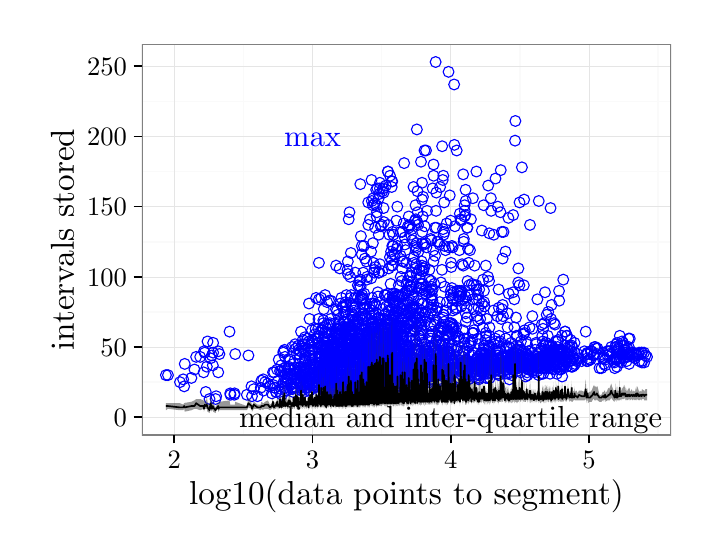
\begin{tikzpicture}[x=1pt,y=1pt]
\definecolor[named]{fillColor}{rgb}{1.00,1.00,1.00}
\path[use as bounding box,fill=fillColor,fill opacity=0.00] (0,0) rectangle (238.49,180.67);
\begin{scope}
\path[clip] (  0.00,  0.00) rectangle (238.49,180.67);
\definecolor[named]{drawColor}{rgb}{1.00,1.00,1.00}
\definecolor[named]{fillColor}{rgb}{1.00,1.00,1.00}

\path[draw=drawColor,line width= 0.6pt,line join=round,line cap=round,fill=fillColor] (  0.00,  0.00) rectangle (238.49,180.68);
\end{scope}
\begin{scope}
\path[clip] ( 41.26, 33.48) rectangle (232.49,174.67);
\definecolor[named]{fillColor}{rgb}{1.00,1.00,1.00}

\path[fill=fillColor] ( 41.26, 33.48) rectangle (232.49,174.67);
\definecolor[named]{drawColor}{rgb}{0.98,0.98,0.98}

\path[draw=drawColor,line width= 0.6pt,line join=round] ( 41.26, 52.58) --
	(232.49, 52.58);

\path[draw=drawColor,line width= 0.6pt,line join=round] ( 41.26, 77.95) --
	(232.49, 77.95);

\path[draw=drawColor,line width= 0.6pt,line join=round] ( 41.26,103.31) --
	(232.49,103.31);

\path[draw=drawColor,line width= 0.6pt,line join=round] ( 41.26,128.68) --
	(232.49,128.68);

\path[draw=drawColor,line width= 0.6pt,line join=round] ( 41.26,154.05) --
	(232.49,154.05);

\path[draw=drawColor,line width= 0.6pt,line join=round] ( 77.95, 33.48) --
	( 77.95,174.67);

\path[draw=drawColor,line width= 0.6pt,line join=round] (127.89, 33.48) --
	(127.89,174.67);

\path[draw=drawColor,line width= 0.6pt,line join=round] (177.84, 33.48) --
	(177.84,174.67);

\path[draw=drawColor,line width= 0.6pt,line join=round] (227.78, 33.48) --
	(227.78,174.67);
\definecolor[named]{drawColor}{rgb}{0.90,0.90,0.90}

\path[draw=drawColor,line width= 0.2pt,line join=round] ( 41.26, 39.89) --
	(232.49, 39.89);

\path[draw=drawColor,line width= 0.2pt,line join=round] ( 41.26, 65.26) --
	(232.49, 65.26);

\path[draw=drawColor,line width= 0.2pt,line join=round] ( 41.26, 90.63) --
	(232.49, 90.63);

\path[draw=drawColor,line width= 0.2pt,line join=round] ( 41.26,116.00) --
	(232.49,116.00);

\path[draw=drawColor,line width= 0.2pt,line join=round] ( 41.26,141.37) --
	(232.49,141.37);

\path[draw=drawColor,line width= 0.2pt,line join=round] ( 41.26,166.73) --
	(232.49,166.73);

\path[draw=drawColor,line width= 0.2pt,line join=round] ( 52.97, 33.48) --
	( 52.97,174.67);

\path[draw=drawColor,line width= 0.2pt,line join=round] (102.92, 33.48) --
	(102.92,174.67);

\path[draw=drawColor,line width= 0.2pt,line join=round] (152.86, 33.48) --
	(152.86,174.67);

\path[draw=drawColor,line width= 0.2pt,line join=round] (202.81, 33.48) --
	(202.81,174.67);
\definecolor[named]{drawColor}{rgb}{0.00,0.00,1.00}

\node[text=drawColor,anchor=base,inner sep=0pt, outer sep=0pt, scale=  1.10] at (102.92,137.57) {max};
\definecolor[named]{drawColor}{rgb}{0.00,0.00,0.00}

\node[text=drawColor,anchor=base,inner sep=0pt, outer sep=0pt, scale=  1.10] at (152.86, 36.09) {median and inter-quartile range};
\definecolor[named]{drawColor}{rgb}{0.00,0.00,1.00}

\path[draw=drawColor,line width= 0.4pt,line join=round,line cap=round] ( 49.95, 55.12) circle (  1.96);

\path[draw=drawColor,line width= 0.4pt,line join=round,line cap=round] ( 50.69, 55.12) circle (  1.96);

\path[draw=drawColor,line width= 0.4pt,line join=round,line cap=round] ( 55.04, 52.58) circle (  1.96);

\path[draw=drawColor,line width= 0.4pt,line join=round,line cap=round] ( 56.19, 53.59) circle (  1.96);

\path[draw=drawColor,line width= 0.4pt,line join=round,line cap=round] ( 56.56, 51.06) circle (  1.96);

\path[draw=drawColor,line width= 0.4pt,line join=round,line cap=round] ( 56.75, 59.17) circle (  1.96);

\path[draw=drawColor,line width= 0.4pt,line join=round,line cap=round] ( 59.16, 54.10) circle (  1.96);

\path[draw=drawColor,line width= 0.4pt,line join=round,line cap=round] ( 60.27, 57.14) circle (  1.96);

\path[draw=drawColor,line width= 0.4pt,line join=round,line cap=round] ( 60.88, 61.71) circle (  1.96);

\path[draw=drawColor,line width= 0.4pt,line join=round,line cap=round] ( 62.34, 61.71) circle (  1.96);

\path[draw=drawColor,line width= 0.4pt,line join=round,line cap=round] ( 63.57, 56.13) circle (  1.96);

\path[draw=drawColor,line width= 0.4pt,line join=round,line cap=round] ( 63.70, 63.74) circle (  1.96);

\path[draw=drawColor,line width= 0.4pt,line join=round,line cap=round] ( 63.97, 63.23) circle (  1.96);

\path[draw=drawColor,line width= 0.4pt,line join=round,line cap=round] ( 64.36, 49.03) circle (  1.96);

\path[draw=drawColor,line width= 0.4pt,line join=round,line cap=round] ( 64.74, 58.16) circle (  1.96);

\path[draw=drawColor,line width= 0.4pt,line join=round,line cap=round] ( 64.99, 67.29) circle (  1.96);

\path[draw=drawColor,line width= 0.4pt,line join=round,line cap=round] ( 65.72, 46.49) circle (  1.96);

\path[draw=drawColor,line width= 0.4pt,line join=round,line cap=round] ( 66.08, 61.20) circle (  1.96);

\path[draw=drawColor,line width= 0.4pt,line join=round,line cap=round] ( 66.55, 62.22) circle (  1.96);

\path[draw=drawColor,line width= 0.4pt,line join=round,line cap=round] ( 66.90, 58.67) circle (  1.96);

\path[draw=drawColor,line width= 0.4pt,line join=round,line cap=round] ( 67.01, 66.78) circle (  1.96);

\path[draw=drawColor,line width= 0.4pt,line join=round,line cap=round] ( 67.01, 63.23) circle (  1.96);

\path[draw=drawColor,line width= 0.4pt,line join=round,line cap=round] ( 67.90, 46.49) circle (  1.96);

\path[draw=drawColor,line width= 0.4pt,line join=round,line cap=round] ( 68.12, 47.50) circle (  1.96);

\path[draw=drawColor,line width= 0.4pt,line join=round,line cap=round] ( 68.86, 56.13) circle (  1.96);

\path[draw=drawColor,line width= 0.4pt,line join=round,line cap=round] ( 68.86, 63.74) circle (  1.96);

\path[draw=drawColor,line width= 0.4pt,line join=round,line cap=round] ( 69.27, 62.73) circle (  1.96);

\path[draw=drawColor,line width= 0.4pt,line join=round,line cap=round] ( 72.94, 70.84) circle (  1.96);

\path[draw=drawColor,line width= 0.4pt,line join=round,line cap=round] ( 73.19, 48.52) circle (  1.96);

\path[draw=drawColor,line width= 0.4pt,line join=round,line cap=round] ( 73.28, 48.01) circle (  1.96);

\path[draw=drawColor,line width= 0.4pt,line join=round,line cap=round] ( 74.68, 48.01) circle (  1.96);

\path[draw=drawColor,line width= 0.4pt,line join=round,line cap=round] ( 74.76, 48.52) circle (  1.96);

\path[draw=drawColor,line width= 0.4pt,line join=round,line cap=round] ( 75.00, 62.73) circle (  1.96);

\path[draw=drawColor,line width= 0.4pt,line join=round,line cap=round] ( 79.20, 48.01) circle (  1.96);

\path[draw=drawColor,line width= 0.4pt,line join=round,line cap=round] ( 79.77, 62.22) circle (  1.96);

\path[draw=drawColor,line width= 0.4pt,line join=round,line cap=round] ( 80.88, 51.06) circle (  1.96);

\path[draw=drawColor,line width= 0.4pt,line join=round,line cap=round] ( 81.06, 47.50) circle (  1.96);

\path[draw=drawColor,line width= 0.4pt,line join=round,line cap=round] ( 81.70, 50.04) circle (  1.96);

\path[draw=drawColor,line width= 0.4pt,line join=round,line cap=round] ( 83.04, 47.50) circle (  1.96);

\path[draw=drawColor,line width= 0.4pt,line join=round,line cap=round] ( 84.21, 50.55) circle (  1.96);

\path[draw=drawColor,line width= 0.4pt,line join=round,line cap=round] ( 84.46, 53.09) circle (  1.96);

\path[draw=drawColor,line width= 0.4pt,line join=round,line cap=round] ( 85.11, 53.59) circle (  1.96);

\path[draw=drawColor,line width= 0.4pt,line join=round,line cap=round] ( 85.26, 49.53) circle (  1.96);

\path[draw=drawColor,line width= 0.4pt,line join=round,line cap=round] ( 85.79, 52.58) circle (  1.96);

\path[draw=drawColor,line width= 0.4pt,line join=round,line cap=round] ( 86.82, 52.07) circle (  1.96);

\path[draw=drawColor,line width= 0.4pt,line join=round,line cap=round] ( 87.53, 51.06) circle (  1.96);

\path[draw=drawColor,line width= 0.4pt,line join=round,line cap=round] ( 88.27, 48.52) circle (  1.96);

\path[draw=drawColor,line width= 0.4pt,line join=round,line cap=round] ( 88.65, 56.13) circle (  1.96);

\path[draw=drawColor,line width= 0.4pt,line join=round,line cap=round] ( 88.69, 51.56) circle (  1.96);

\path[draw=drawColor,line width= 0.4pt,line join=round,line cap=round] ( 89.07, 56.13) circle (  1.96);

\path[draw=drawColor,line width= 0.4pt,line join=round,line cap=round] ( 89.19, 50.55) circle (  1.96);

\path[draw=drawColor,line width= 0.4pt,line join=round,line cap=round] ( 89.35, 50.55) circle (  1.96);

\path[draw=drawColor,line width= 0.4pt,line join=round,line cap=round] ( 89.75, 49.03) circle (  1.96);

\path[draw=drawColor,line width= 0.4pt,line join=round,line cap=round] ( 89.79, 49.03) circle (  1.96);

\path[draw=drawColor,line width= 0.4pt,line join=round,line cap=round] ( 90.15, 57.14) circle (  1.96);

\path[draw=drawColor,line width= 0.4pt,line join=round,line cap=round] ( 90.42, 53.09) circle (  1.96);

\path[draw=drawColor,line width= 0.4pt,line join=round,line cap=round] ( 90.73, 60.70) circle (  1.96);

\path[draw=drawColor,line width= 0.4pt,line join=round,line cap=round] ( 91.07, 49.03) circle (  1.96);

\path[draw=drawColor,line width= 0.4pt,line join=round,line cap=round] ( 91.18, 56.64) circle (  1.96);

\path[draw=drawColor,line width= 0.4pt,line join=round,line cap=round] ( 91.58, 50.04) circle (  1.96);

\path[draw=drawColor,line width= 0.4pt,line join=round,line cap=round] ( 91.62, 58.67) circle (  1.96);

\path[draw=drawColor,line width= 0.4pt,line join=round,line cap=round] ( 91.66, 56.64) circle (  1.96);

\path[draw=drawColor,line width= 0.4pt,line join=round,line cap=round] ( 91.84, 48.01) circle (  1.96);

\path[draw=drawColor,line width= 0.4pt,line join=round,line cap=round] ( 91.84, 51.06) circle (  1.96);

\path[draw=drawColor,line width= 0.4pt,line join=round,line cap=round] ( 92.37, 63.23) circle (  1.96);

\path[draw=drawColor,line width= 0.4pt,line join=round,line cap=round] ( 92.45, 63.74) circle (  1.96);

\path[draw=drawColor,line width= 0.4pt,line join=round,line cap=round] ( 92.45, 52.58) circle (  1.96);

\path[draw=drawColor,line width= 0.4pt,line join=round,line cap=round] ( 92.62, 56.64) circle (  1.96);

\path[draw=drawColor,line width= 0.4pt,line join=round,line cap=round] ( 92.66, 54.61) circle (  1.96);

\path[draw=drawColor,line width= 0.4pt,line join=round,line cap=round] ( 92.83, 64.25) circle (  1.96);

\path[draw=drawColor,line width= 0.4pt,line join=round,line cap=round] ( 92.83, 50.55) circle (  1.96);

\path[draw=drawColor,line width= 0.4pt,line join=round,line cap=round] ( 92.93, 57.65) circle (  1.96);

\path[draw=drawColor,line width= 0.4pt,line join=round,line cap=round] ( 93.00, 61.71) circle (  1.96);

\path[draw=drawColor,line width= 0.4pt,line join=round,line cap=round] ( 93.07, 49.53) circle (  1.96);

\path[draw=drawColor,line width= 0.4pt,line join=round,line cap=round] ( 93.10, 53.09) circle (  1.96);

\path[draw=drawColor,line width= 0.4pt,line join=round,line cap=round] ( 93.14, 52.07) circle (  1.96);

\path[draw=drawColor,line width= 0.4pt,line join=round,line cap=round] ( 93.24, 55.62) circle (  1.96);

\path[draw=drawColor,line width= 0.4pt,line join=round,line cap=round] ( 93.74, 54.10) circle (  1.96);

\path[draw=drawColor,line width= 0.4pt,line join=round,line cap=round] ( 93.77, 49.53) circle (  1.96);

\path[draw=drawColor,line width= 0.4pt,line join=round,line cap=round] ( 93.77, 52.58) circle (  1.96);

\path[draw=drawColor,line width= 0.4pt,line join=round,line cap=round] ( 93.87, 55.12) circle (  1.96);

\path[draw=drawColor,line width= 0.4pt,line join=round,line cap=round] ( 93.94, 53.59) circle (  1.96);

\path[draw=drawColor,line width= 0.4pt,line join=round,line cap=round] ( 94.07, 57.65) circle (  1.96);

\path[draw=drawColor,line width= 0.4pt,line join=round,line cap=round] ( 94.30, 58.16) circle (  1.96);

\path[draw=drawColor,line width= 0.4pt,line join=round,line cap=round] ( 94.33, 57.65) circle (  1.96);

\path[draw=drawColor,line width= 0.4pt,line join=round,line cap=round] ( 94.43, 60.19) circle (  1.96);

\path[draw=drawColor,line width= 0.4pt,line join=round,line cap=round] ( 94.55, 55.62) circle (  1.96);

\path[draw=drawColor,line width= 0.4pt,line join=round,line cap=round] ( 94.93, 60.70) circle (  1.96);

\path[draw=drawColor,line width= 0.4pt,line join=round,line cap=round] ( 95.00, 51.56) circle (  1.96);

\path[draw=drawColor,line width= 0.4pt,line join=round,line cap=round] ( 95.21, 55.12) circle (  1.96);

\path[draw=drawColor,line width= 0.4pt,line join=round,line cap=round] ( 95.24, 53.59) circle (  1.96);

\path[draw=drawColor,line width= 0.4pt,line join=round,line cap=round] ( 95.37, 52.07) circle (  1.96);

\path[draw=drawColor,line width= 0.4pt,line join=round,line cap=round] ( 95.52, 50.55) circle (  1.96);

\path[draw=drawColor,line width= 0.4pt,line join=round,line cap=round] ( 95.55, 65.26) circle (  1.96);

\path[draw=drawColor,line width= 0.4pt,line join=round,line cap=round] ( 95.64, 50.04) circle (  1.96);

\path[draw=drawColor,line width= 0.4pt,line join=round,line cap=round] ( 95.82, 55.12) circle (  1.96);

\path[draw=drawColor,line width= 0.4pt,line join=round,line cap=round] ( 95.82, 50.55) circle (  1.96);

\path[draw=drawColor,line width= 0.4pt,line join=round,line cap=round] ( 95.91, 49.03) circle (  1.96);

\path[draw=drawColor,line width= 0.4pt,line join=round,line cap=round] ( 95.91, 50.55) circle (  1.96);

\path[draw=drawColor,line width= 0.4pt,line join=round,line cap=round] ( 96.09, 59.17) circle (  1.96);

\path[draw=drawColor,line width= 0.4pt,line join=round,line cap=round] ( 96.12, 51.06) circle (  1.96);

\path[draw=drawColor,line width= 0.4pt,line join=round,line cap=round] ( 96.30, 55.62) circle (  1.96);

\path[draw=drawColor,line width= 0.4pt,line join=round,line cap=round] ( 96.36, 50.55) circle (  1.96);

\path[draw=drawColor,line width= 0.4pt,line join=round,line cap=round] ( 96.65, 57.65) circle (  1.96);

\path[draw=drawColor,line width= 0.4pt,line join=round,line cap=round] ( 96.65, 66.28) circle (  1.96);

\path[draw=drawColor,line width= 0.4pt,line join=round,line cap=round] ( 96.91, 64.76) circle (  1.96);

\path[draw=drawColor,line width= 0.4pt,line join=round,line cap=round] ( 97.11, 50.55) circle (  1.96);

\path[draw=drawColor,line width= 0.4pt,line join=round,line cap=round] ( 97.19, 52.07) circle (  1.96);

\path[draw=drawColor,line width= 0.4pt,line join=round,line cap=round] ( 97.25, 56.13) circle (  1.96);

\path[draw=drawColor,line width= 0.4pt,line join=round,line cap=round] ( 97.31, 62.73) circle (  1.96);

\path[draw=drawColor,line width= 0.4pt,line join=round,line cap=round] ( 97.42, 56.64) circle (  1.96);

\path[draw=drawColor,line width= 0.4pt,line join=round,line cap=round] ( 97.81, 52.58) circle (  1.96);

\path[draw=drawColor,line width= 0.4pt,line join=round,line cap=round] ( 97.81, 65.77) circle (  1.96);

\path[draw=drawColor,line width= 0.4pt,line join=round,line cap=round] ( 97.94, 57.65) circle (  1.96);

\path[draw=drawColor,line width= 0.4pt,line join=round,line cap=round] ( 98.00, 64.25) circle (  1.96);

\path[draw=drawColor,line width= 0.4pt,line join=round,line cap=round] ( 98.02, 55.62) circle (  1.96);

\path[draw=drawColor,line width= 0.4pt,line join=round,line cap=round] ( 98.13, 62.73) circle (  1.96);

\path[draw=drawColor,line width= 0.4pt,line join=round,line cap=round] ( 98.21, 61.20) circle (  1.96);

\path[draw=drawColor,line width= 0.4pt,line join=round,line cap=round] ( 98.21, 57.65) circle (  1.96);

\path[draw=drawColor,line width= 0.4pt,line join=round,line cap=round] ( 98.38, 52.58) circle (  1.96);

\path[draw=drawColor,line width= 0.4pt,line join=round,line cap=round] ( 98.40, 54.61) circle (  1.96);

\path[draw=drawColor,line width= 0.4pt,line join=round,line cap=round] ( 98.43, 63.74) circle (  1.96);

\path[draw=drawColor,line width= 0.4pt,line join=round,line cap=round] ( 98.48, 52.07) circle (  1.96);

\path[draw=drawColor,line width= 0.4pt,line join=round,line cap=round] ( 98.54, 56.64) circle (  1.96);

\path[draw=drawColor,line width= 0.4pt,line join=round,line cap=round] ( 98.69, 50.55) circle (  1.96);

\path[draw=drawColor,line width= 0.4pt,line join=round,line cap=round] ( 98.77, 70.84) circle (  1.96);

\path[draw=drawColor,line width= 0.4pt,line join=round,line cap=round] ( 98.80, 58.16) circle (  1.96);

\path[draw=drawColor,line width= 0.4pt,line join=round,line cap=round] ( 98.93, 50.55) circle (  1.96);

\path[draw=drawColor,line width= 0.4pt,line join=round,line cap=round] ( 98.98, 49.53) circle (  1.96);

\path[draw=drawColor,line width= 0.4pt,line join=round,line cap=round] ( 98.98, 55.12) circle (  1.96);

\path[draw=drawColor,line width= 0.4pt,line join=round,line cap=round] ( 99.09, 54.61) circle (  1.96);

\path[draw=drawColor,line width= 0.4pt,line join=round,line cap=round] ( 99.27, 66.28) circle (  1.96);

\path[draw=drawColor,line width= 0.4pt,line join=round,line cap=round] ( 99.29, 54.61) circle (  1.96);

\path[draw=drawColor,line width= 0.4pt,line join=round,line cap=round] ( 99.29, 56.13) circle (  1.96);

\path[draw=drawColor,line width= 0.4pt,line join=round,line cap=round] ( 99.34, 56.13) circle (  1.96);

\path[draw=drawColor,line width= 0.4pt,line join=round,line cap=round] ( 99.39, 67.80) circle (  1.96);

\path[draw=drawColor,line width= 0.4pt,line join=round,line cap=round] ( 99.52, 51.56) circle (  1.96);

\path[draw=drawColor,line width= 0.4pt,line join=round,line cap=round] ( 99.52, 64.76) circle (  1.96);

\path[draw=drawColor,line width= 0.4pt,line join=round,line cap=round] ( 99.62, 55.12) circle (  1.96);

\path[draw=drawColor,line width= 0.4pt,line join=round,line cap=round] ( 99.75, 53.09) circle (  1.96);

\path[draw=drawColor,line width= 0.4pt,line join=round,line cap=round] ( 99.75, 52.07) circle (  1.96);

\path[draw=drawColor,line width= 0.4pt,line join=round,line cap=round] ( 99.82, 57.65) circle (  1.96);

\path[draw=drawColor,line width= 0.4pt,line join=round,line cap=round] ( 99.92, 49.03) circle (  1.96);

\path[draw=drawColor,line width= 0.4pt,line join=round,line cap=round] ( 99.92, 60.70) circle (  1.96);

\path[draw=drawColor,line width= 0.4pt,line join=round,line cap=round] (100.00, 56.64) circle (  1.96);

\path[draw=drawColor,line width= 0.4pt,line join=round,line cap=round] (100.00, 56.13) circle (  1.96);

\path[draw=drawColor,line width= 0.4pt,line join=round,line cap=round] (100.17, 66.28) circle (  1.96);

\path[draw=drawColor,line width= 0.4pt,line join=round,line cap=round] (100.17, 56.13) circle (  1.96);

\path[draw=drawColor,line width= 0.4pt,line join=round,line cap=round] (100.20, 68.81) circle (  1.96);

\path[draw=drawColor,line width= 0.4pt,line join=round,line cap=round] (100.22, 57.65) circle (  1.96);

\path[draw=drawColor,line width= 0.4pt,line join=round,line cap=round] (100.27, 63.74) circle (  1.96);

\path[draw=drawColor,line width= 0.4pt,line join=round,line cap=round] (100.27, 50.55) circle (  1.96);

\path[draw=drawColor,line width= 0.4pt,line join=round,line cap=round] (100.29, 62.22) circle (  1.96);

\path[draw=drawColor,line width= 0.4pt,line join=round,line cap=round] (100.29, 60.19) circle (  1.96);

\path[draw=drawColor,line width= 0.4pt,line join=round,line cap=round] (100.44, 56.64) circle (  1.96);

\path[draw=drawColor,line width= 0.4pt,line join=round,line cap=round] (100.51, 60.19) circle (  1.96);

\path[draw=drawColor,line width= 0.4pt,line join=round,line cap=round] (100.54, 51.56) circle (  1.96);

\path[draw=drawColor,line width= 0.4pt,line join=round,line cap=round] (100.56, 56.64) circle (  1.96);

\path[draw=drawColor,line width= 0.4pt,line join=round,line cap=round] (100.59, 53.09) circle (  1.96);

\path[draw=drawColor,line width= 0.4pt,line join=round,line cap=round] (100.61, 50.55) circle (  1.96);

\path[draw=drawColor,line width= 0.4pt,line join=round,line cap=round] (100.63, 52.07) circle (  1.96);

\path[draw=drawColor,line width= 0.4pt,line join=round,line cap=round] (100.99, 50.55) circle (  1.96);

\path[draw=drawColor,line width= 0.4pt,line join=round,line cap=round] (101.04, 56.64) circle (  1.96);

\path[draw=drawColor,line width= 0.4pt,line join=round,line cap=round] (101.13, 68.31) circle (  1.96);

\path[draw=drawColor,line width= 0.4pt,line join=round,line cap=round] (101.28, 54.61) circle (  1.96);

\path[draw=drawColor,line width= 0.4pt,line join=round,line cap=round] (101.53, 49.53) circle (  1.96);

\path[draw=drawColor,line width= 0.4pt,line join=round,line cap=round] (101.53, 52.07) circle (  1.96);

\path[draw=drawColor,line width= 0.4pt,line join=round,line cap=round] (101.65, 67.29) circle (  1.96);

\path[draw=drawColor,line width= 0.4pt,line join=round,line cap=round] (101.65, 80.99) circle (  1.96);

\path[draw=drawColor,line width= 0.4pt,line join=round,line cap=round] (101.67, 54.10) circle (  1.96);

\path[draw=drawColor,line width= 0.4pt,line join=round,line cap=round] (101.76, 61.20) circle (  1.96);

\path[draw=drawColor,line width= 0.4pt,line join=round,line cap=round] (101.83, 54.10) circle (  1.96);

\path[draw=drawColor,line width= 0.4pt,line join=round,line cap=round] (101.85, 75.41) circle (  1.96);

\path[draw=drawColor,line width= 0.4pt,line join=round,line cap=round] (101.88, 49.53) circle (  1.96);

\path[draw=drawColor,line width= 0.4pt,line join=round,line cap=round] (101.88, 54.10) circle (  1.96);

\path[draw=drawColor,line width= 0.4pt,line join=round,line cap=round] (101.92, 51.56) circle (  1.96);

\path[draw=drawColor,line width= 0.4pt,line join=round,line cap=round] (101.97, 59.17) circle (  1.96);

\path[draw=drawColor,line width= 0.4pt,line join=round,line cap=round] (101.97, 61.20) circle (  1.96);

\path[draw=drawColor,line width= 0.4pt,line join=round,line cap=round] (102.01, 59.17) circle (  1.96);

\path[draw=drawColor,line width= 0.4pt,line join=round,line cap=round] (102.01, 65.77) circle (  1.96);

\path[draw=drawColor,line width= 0.4pt,line join=round,line cap=round] (102.03, 62.22) circle (  1.96);

\path[draw=drawColor,line width= 0.4pt,line join=round,line cap=round] (102.06, 63.23) circle (  1.96);

\path[draw=drawColor,line width= 0.4pt,line join=round,line cap=round] (102.10, 57.65) circle (  1.96);

\path[draw=drawColor,line width= 0.4pt,line join=round,line cap=round] (102.48, 61.71) circle (  1.96);

\path[draw=drawColor,line width= 0.4pt,line join=round,line cap=round] (102.64, 55.62) circle (  1.96);

\path[draw=drawColor,line width= 0.4pt,line join=round,line cap=round] (102.68, 64.25) circle (  1.96);

\path[draw=drawColor,line width= 0.4pt,line join=round,line cap=round] (102.70, 52.07) circle (  1.96);

\path[draw=drawColor,line width= 0.4pt,line join=round,line cap=round] (102.72, 71.35) circle (  1.96);

\path[draw=drawColor,line width= 0.4pt,line join=round,line cap=round] (102.75, 60.70) circle (  1.96);

\path[draw=drawColor,line width= 0.4pt,line join=round,line cap=round] (102.77, 60.70) circle (  1.96);

\path[draw=drawColor,line width= 0.4pt,line join=round,line cap=round] (102.81, 67.80) circle (  1.96);

\path[draw=drawColor,line width= 0.4pt,line join=round,line cap=round] (102.98, 56.64) circle (  1.96);

\path[draw=drawColor,line width= 0.4pt,line join=round,line cap=round] (103.01, 67.29) circle (  1.96);

\path[draw=drawColor,line width= 0.4pt,line join=round,line cap=round] (103.11, 51.56) circle (  1.96);

\path[draw=drawColor,line width= 0.4pt,line join=round,line cap=round] (103.18, 63.23) circle (  1.96);

\path[draw=drawColor,line width= 0.4pt,line join=round,line cap=round] (103.20, 50.55) circle (  1.96);

\path[draw=drawColor,line width= 0.4pt,line join=round,line cap=round] (103.26, 56.13) circle (  1.96);

\path[draw=drawColor,line width= 0.4pt,line join=round,line cap=round] (103.35, 59.17) circle (  1.96);

\path[draw=drawColor,line width= 0.4pt,line join=round,line cap=round] (103.43, 55.12) circle (  1.96);

\path[draw=drawColor,line width= 0.4pt,line join=round,line cap=round] (103.48, 50.55) circle (  1.96);

\path[draw=drawColor,line width= 0.4pt,line join=round,line cap=round] (103.54, 57.14) circle (  1.96);

\path[draw=drawColor,line width= 0.4pt,line join=round,line cap=round] (103.69, 69.83) circle (  1.96);

\path[draw=drawColor,line width= 0.4pt,line join=round,line cap=round] (103.71, 58.67) circle (  1.96);

\path[draw=drawColor,line width= 0.4pt,line join=round,line cap=round] (103.73, 51.56) circle (  1.96);

\path[draw=drawColor,line width= 0.4pt,line join=round,line cap=round] (103.96, 61.20) circle (  1.96);

\path[draw=drawColor,line width= 0.4pt,line join=round,line cap=round] (104.02, 51.06) circle (  1.96);

\path[draw=drawColor,line width= 0.4pt,line join=round,line cap=round] (104.06, 71.86) circle (  1.96);

\path[draw=drawColor,line width= 0.4pt,line join=round,line cap=round] (104.14, 68.31) circle (  1.96);

\path[draw=drawColor,line width= 0.4pt,line join=round,line cap=round] (104.16, 56.13) circle (  1.96);

\path[draw=drawColor,line width= 0.4pt,line join=round,line cap=round] (104.16, 54.10) circle (  1.96);

\path[draw=drawColor,line width= 0.4pt,line join=round,line cap=round] (104.18, 68.31) circle (  1.96);

\path[draw=drawColor,line width= 0.4pt,line join=round,line cap=round] (104.18, 55.12) circle (  1.96);

\path[draw=drawColor,line width= 0.4pt,line join=round,line cap=round] (104.18, 53.09) circle (  1.96);

\path[draw=drawColor,line width= 0.4pt,line join=round,line cap=round] (104.20, 54.61) circle (  1.96);

\path[draw=drawColor,line width= 0.4pt,line join=round,line cap=round] (104.22, 83.02) circle (  1.96);

\path[draw=drawColor,line width= 0.4pt,line join=round,line cap=round] (104.41, 51.06) circle (  1.96);

\path[draw=drawColor,line width= 0.4pt,line join=round,line cap=round] (104.47, 58.16) circle (  1.96);

\path[draw=drawColor,line width= 0.4pt,line join=round,line cap=round] (104.79, 51.06) circle (  1.96);

\path[draw=drawColor,line width= 0.4pt,line join=round,line cap=round] (104.83, 65.26) circle (  1.96);

\path[draw=drawColor,line width= 0.4pt,line join=round,line cap=round] (104.97, 66.78) circle (  1.96);

\path[draw=drawColor,line width= 0.4pt,line join=round,line cap=round] (104.97, 57.14) circle (  1.96);

\path[draw=drawColor,line width= 0.4pt,line join=round,line cap=round] (105.01, 69.32) circle (  1.96);

\path[draw=drawColor,line width= 0.4pt,line join=round,line cap=round] (105.03, 71.86) circle (  1.96);

\path[draw=drawColor,line width= 0.4pt,line join=round,line cap=round] (105.14, 56.64) circle (  1.96);

\path[draw=drawColor,line width= 0.4pt,line join=round,line cap=round] (105.14, 75.41) circle (  1.96);

\path[draw=drawColor,line width= 0.4pt,line join=round,line cap=round] (105.24, 95.70) circle (  1.96);

\path[draw=drawColor,line width= 0.4pt,line join=round,line cap=round] (105.26, 52.07) circle (  1.96);

\path[draw=drawColor,line width= 0.4pt,line join=round,line cap=round] (105.26, 82.51) circle (  1.96);

\path[draw=drawColor,line width= 0.4pt,line join=round,line cap=round] (105.28, 58.16) circle (  1.96);

\path[draw=drawColor,line width= 0.4pt,line join=round,line cap=round] (105.34, 56.64) circle (  1.96);

\path[draw=drawColor,line width= 0.4pt,line join=round,line cap=round] (105.38, 63.23) circle (  1.96);

\path[draw=drawColor,line width= 0.4pt,line join=round,line cap=round] (105.42, 70.34) circle (  1.96);

\path[draw=drawColor,line width= 0.4pt,line join=round,line cap=round] (105.42, 61.20) circle (  1.96);

\path[draw=drawColor,line width= 0.4pt,line join=round,line cap=round] (105.63, 51.56) circle (  1.96);

\path[draw=drawColor,line width= 0.4pt,line join=round,line cap=round] (105.70, 62.73) circle (  1.96);

\path[draw=drawColor,line width= 0.4pt,line join=round,line cap=round] (105.78, 58.67) circle (  1.96);

\path[draw=drawColor,line width= 0.4pt,line join=round,line cap=round] (105.84, 54.10) circle (  1.96);

\path[draw=drawColor,line width= 0.4pt,line join=round,line cap=round] (105.89, 61.71) circle (  1.96);

\path[draw=drawColor,line width= 0.4pt,line join=round,line cap=round] (105.91, 49.03) circle (  1.96);

\path[draw=drawColor,line width= 0.4pt,line join=round,line cap=round] (105.97, 56.13) circle (  1.96);

\path[draw=drawColor,line width= 0.4pt,line join=round,line cap=round] (106.01, 54.10) circle (  1.96);

\path[draw=drawColor,line width= 0.4pt,line join=round,line cap=round] (106.05, 83.02) circle (  1.96);

\path[draw=drawColor,line width= 0.4pt,line join=round,line cap=round] (106.10, 65.26) circle (  1.96);

\path[draw=drawColor,line width= 0.4pt,line join=round,line cap=round] (106.14, 51.06) circle (  1.96);

\path[draw=drawColor,line width= 0.4pt,line join=round,line cap=round] (106.18, 57.65) circle (  1.96);

\path[draw=drawColor,line width= 0.4pt,line join=round,line cap=round] (106.25, 65.26) circle (  1.96);

\path[draw=drawColor,line width= 0.4pt,line join=round,line cap=round] (106.27, 55.12) circle (  1.96);

\path[draw=drawColor,line width= 0.4pt,line join=round,line cap=round] (106.29, 53.59) circle (  1.96);

\path[draw=drawColor,line width= 0.4pt,line join=round,line cap=round] (106.29, 56.64) circle (  1.96);

\path[draw=drawColor,line width= 0.4pt,line join=round,line cap=round] (106.31, 64.25) circle (  1.96);

\path[draw=drawColor,line width= 0.4pt,line join=round,line cap=round] (106.31, 57.14) circle (  1.96);

\path[draw=drawColor,line width= 0.4pt,line join=round,line cap=round] (106.33, 65.77) circle (  1.96);

\path[draw=drawColor,line width= 0.4pt,line join=round,line cap=round] (106.36, 64.25) circle (  1.96);

\path[draw=drawColor,line width= 0.4pt,line join=round,line cap=round] (106.44, 64.25) circle (  1.96);

\path[draw=drawColor,line width= 0.4pt,line join=round,line cap=round] (106.49, 60.19) circle (  1.96);

\path[draw=drawColor,line width= 0.4pt,line join=round,line cap=round] (106.55, 53.09) circle (  1.96);

\path[draw=drawColor,line width= 0.4pt,line join=round,line cap=round] (106.55, 53.09) circle (  1.96);

\path[draw=drawColor,line width= 0.4pt,line join=round,line cap=round] (106.56, 58.16) circle (  1.96);

\path[draw=drawColor,line width= 0.4pt,line join=round,line cap=round] (106.58, 71.35) circle (  1.96);

\path[draw=drawColor,line width= 0.4pt,line join=round,line cap=round] (106.64, 72.37) circle (  1.96);

\path[draw=drawColor,line width= 0.4pt,line join=round,line cap=round] (106.73, 68.31) circle (  1.96);

\path[draw=drawColor,line width= 0.4pt,line join=round,line cap=round] (106.75, 52.58) circle (  1.96);

\path[draw=drawColor,line width= 0.4pt,line join=round,line cap=round] (106.80, 53.09) circle (  1.96);

\path[draw=drawColor,line width= 0.4pt,line join=round,line cap=round] (106.84, 74.90) circle (  1.96);

\path[draw=drawColor,line width= 0.4pt,line join=round,line cap=round] (106.89, 65.26) circle (  1.96);

\path[draw=drawColor,line width= 0.4pt,line join=round,line cap=round] (106.91, 65.26) circle (  1.96);

\path[draw=drawColor,line width= 0.4pt,line join=round,line cap=round] (106.91, 73.89) circle (  1.96);

\path[draw=drawColor,line width= 0.4pt,line join=round,line cap=round] (107.00, 78.96) circle (  1.96);

\path[draw=drawColor,line width= 0.4pt,line join=round,line cap=round] (107.00, 59.17) circle (  1.96);

\path[draw=drawColor,line width= 0.4pt,line join=round,line cap=round] (107.00, 66.78) circle (  1.96);

\path[draw=drawColor,line width= 0.4pt,line join=round,line cap=round] (107.09, 53.59) circle (  1.96);

\path[draw=drawColor,line width= 0.4pt,line join=round,line cap=round] (107.16, 68.81) circle (  1.96);

\path[draw=drawColor,line width= 0.4pt,line join=round,line cap=round] (107.18, 52.58) circle (  1.96);

\path[draw=drawColor,line width= 0.4pt,line join=round,line cap=round] (107.25, 61.20) circle (  1.96);

\path[draw=drawColor,line width= 0.4pt,line join=round,line cap=round] (107.32, 49.53) circle (  1.96);

\path[draw=drawColor,line width= 0.4pt,line join=round,line cap=round] (107.32, 61.20) circle (  1.96);

\path[draw=drawColor,line width= 0.4pt,line join=round,line cap=round] (107.34, 64.25) circle (  1.96);

\path[draw=drawColor,line width= 0.4pt,line join=round,line cap=round] (107.39, 63.74) circle (  1.96);

\path[draw=drawColor,line width= 0.4pt,line join=round,line cap=round] (107.43, 63.74) circle (  1.96);

\path[draw=drawColor,line width= 0.4pt,line join=round,line cap=round] (107.46, 53.59) circle (  1.96);

\path[draw=drawColor,line width= 0.4pt,line join=round,line cap=round] (107.48, 70.84) circle (  1.96);

\path[draw=drawColor,line width= 0.4pt,line join=round,line cap=round] (107.48, 84.03) circle (  1.96);

\path[draw=drawColor,line width= 0.4pt,line join=round,line cap=round] (107.52, 49.03) circle (  1.96);

\path[draw=drawColor,line width= 0.4pt,line join=round,line cap=round] (107.52, 58.67) circle (  1.96);

\path[draw=drawColor,line width= 0.4pt,line join=round,line cap=round] (107.53, 58.16) circle (  1.96);

\path[draw=drawColor,line width= 0.4pt,line join=round,line cap=round] (107.57, 59.17) circle (  1.96);

\path[draw=drawColor,line width= 0.4pt,line join=round,line cap=round] (107.76, 58.16) circle (  1.96);

\path[draw=drawColor,line width= 0.4pt,line join=round,line cap=round] (107.78, 65.77) circle (  1.96);

\path[draw=drawColor,line width= 0.4pt,line join=round,line cap=round] (107.79, 55.62) circle (  1.96);

\path[draw=drawColor,line width= 0.4pt,line join=round,line cap=round] (107.85, 55.62) circle (  1.96);

\path[draw=drawColor,line width= 0.4pt,line join=round,line cap=round] (107.86, 49.03) circle (  1.96);

\path[draw=drawColor,line width= 0.4pt,line join=round,line cap=round] (107.86, 62.73) circle (  1.96);

\path[draw=drawColor,line width= 0.4pt,line join=round,line cap=round] (107.86, 60.70) circle (  1.96);

\path[draw=drawColor,line width= 0.4pt,line join=round,line cap=round] (107.88, 51.56) circle (  1.96);

\path[draw=drawColor,line width= 0.4pt,line join=round,line cap=round] (107.93, 70.34) circle (  1.96);

\path[draw=drawColor,line width= 0.4pt,line join=round,line cap=round] (107.95, 57.14) circle (  1.96);

\path[draw=drawColor,line width= 0.4pt,line join=round,line cap=round] (107.95, 63.23) circle (  1.96);

\path[draw=drawColor,line width= 0.4pt,line join=round,line cap=round] (107.95, 60.70) circle (  1.96);

\path[draw=drawColor,line width= 0.4pt,line join=round,line cap=round] (107.97, 58.16) circle (  1.96);

\path[draw=drawColor,line width= 0.4pt,line join=round,line cap=round] (108.05, 59.68) circle (  1.96);

\path[draw=drawColor,line width= 0.4pt,line join=round,line cap=round] (108.07, 51.56) circle (  1.96);

\path[draw=drawColor,line width= 0.4pt,line join=round,line cap=round] (108.10, 57.14) circle (  1.96);

\path[draw=drawColor,line width= 0.4pt,line join=round,line cap=round] (108.10, 65.26) circle (  1.96);

\path[draw=drawColor,line width= 0.4pt,line join=round,line cap=round] (108.12, 53.59) circle (  1.96);

\path[draw=drawColor,line width= 0.4pt,line join=round,line cap=round] (108.19, 73.38) circle (  1.96);

\path[draw=drawColor,line width= 0.4pt,line join=round,line cap=round] (108.21, 81.50) circle (  1.96);

\path[draw=drawColor,line width= 0.4pt,line join=round,line cap=round] (108.22, 57.14) circle (  1.96);

\path[draw=drawColor,line width= 0.4pt,line join=round,line cap=round] (108.22, 65.26) circle (  1.96);

\path[draw=drawColor,line width= 0.4pt,line join=round,line cap=round] (108.27, 69.32) circle (  1.96);

\path[draw=drawColor,line width= 0.4pt,line join=round,line cap=round] (108.29, 54.61) circle (  1.96);

\path[draw=drawColor,line width= 0.4pt,line join=round,line cap=round] (108.32, 63.23) circle (  1.96);

\path[draw=drawColor,line width= 0.4pt,line join=round,line cap=round] (108.39, 52.07) circle (  1.96);

\path[draw=drawColor,line width= 0.4pt,line join=round,line cap=round] (108.51, 59.17) circle (  1.96);

\path[draw=drawColor,line width= 0.4pt,line join=round,line cap=round] (108.54, 60.19) circle (  1.96);

\path[draw=drawColor,line width= 0.4pt,line join=round,line cap=round] (108.58, 60.70) circle (  1.96);

\path[draw=drawColor,line width= 0.4pt,line join=round,line cap=round] (108.58, 54.61) circle (  1.96);

\path[draw=drawColor,line width= 0.4pt,line join=round,line cap=round] (108.59, 67.29) circle (  1.96);

\path[draw=drawColor,line width= 0.4pt,line join=round,line cap=round] (108.61, 56.64) circle (  1.96);

\path[draw=drawColor,line width= 0.4pt,line join=round,line cap=round] (108.63, 53.09) circle (  1.96);

\path[draw=drawColor,line width= 0.4pt,line join=round,line cap=round] (108.66, 54.10) circle (  1.96);

\path[draw=drawColor,line width= 0.4pt,line join=round,line cap=round] (108.74, 56.64) circle (  1.96);

\path[draw=drawColor,line width= 0.4pt,line join=round,line cap=round] (108.74, 59.68) circle (  1.96);

\path[draw=drawColor,line width= 0.4pt,line join=round,line cap=round] (108.81, 62.22) circle (  1.96);

\path[draw=drawColor,line width= 0.4pt,line join=round,line cap=round] (108.88, 56.13) circle (  1.96);

\path[draw=drawColor,line width= 0.4pt,line join=round,line cap=round] (108.88, 70.34) circle (  1.96);

\path[draw=drawColor,line width= 0.4pt,line join=round,line cap=round] (108.88, 59.68) circle (  1.96);

\path[draw=drawColor,line width= 0.4pt,line join=round,line cap=round] (108.88, 73.38) circle (  1.96);

\path[draw=drawColor,line width= 0.4pt,line join=round,line cap=round] (108.89, 82.01) circle (  1.96);

\path[draw=drawColor,line width= 0.4pt,line join=round,line cap=round] (109.14, 64.76) circle (  1.96);

\path[draw=drawColor,line width= 0.4pt,line join=round,line cap=round] (109.15, 60.70) circle (  1.96);

\path[draw=drawColor,line width= 0.4pt,line join=round,line cap=round] (109.19, 73.89) circle (  1.96);

\path[draw=drawColor,line width= 0.4pt,line join=round,line cap=round] (109.28, 55.62) circle (  1.96);

\path[draw=drawColor,line width= 0.4pt,line join=round,line cap=round] (109.30, 63.23) circle (  1.96);

\path[draw=drawColor,line width= 0.4pt,line join=round,line cap=round] (109.32, 60.19) circle (  1.96);

\path[draw=drawColor,line width= 0.4pt,line join=round,line cap=round] (109.35, 65.26) circle (  1.96);

\path[draw=drawColor,line width= 0.4pt,line join=round,line cap=round] (109.38, 49.53) circle (  1.96);

\path[draw=drawColor,line width= 0.4pt,line join=round,line cap=round] (109.40, 62.22) circle (  1.96);

\path[draw=drawColor,line width= 0.4pt,line join=round,line cap=round] (109.45, 61.20) circle (  1.96);

\path[draw=drawColor,line width= 0.4pt,line join=round,line cap=round] (109.46, 50.55) circle (  1.96);

\path[draw=drawColor,line width= 0.4pt,line join=round,line cap=round] (109.48, 75.41) circle (  1.96);

\path[draw=drawColor,line width= 0.4pt,line join=round,line cap=round] (109.51, 60.19) circle (  1.96);

\path[draw=drawColor,line width= 0.4pt,line join=round,line cap=round] (109.51, 53.59) circle (  1.96);

\path[draw=drawColor,line width= 0.4pt,line join=round,line cap=round] (109.51, 82.01) circle (  1.96);

\path[draw=drawColor,line width= 0.4pt,line join=round,line cap=round] (109.54, 58.16) circle (  1.96);

\path[draw=drawColor,line width= 0.4pt,line join=round,line cap=round] (109.59, 61.71) circle (  1.96);

\path[draw=drawColor,line width= 0.4pt,line join=round,line cap=round] (109.62, 69.83) circle (  1.96);

\path[draw=drawColor,line width= 0.4pt,line join=round,line cap=round] (109.67, 59.68) circle (  1.96);

\path[draw=drawColor,line width= 0.4pt,line join=round,line cap=round] (109.72, 58.16) circle (  1.96);

\path[draw=drawColor,line width= 0.4pt,line join=round,line cap=round] (109.75, 63.23) circle (  1.96);

\path[draw=drawColor,line width= 0.4pt,line join=round,line cap=round] (109.84, 62.73) circle (  1.96);

\path[draw=drawColor,line width= 0.4pt,line join=round,line cap=round] (109.87, 59.17) circle (  1.96);

\path[draw=drawColor,line width= 0.4pt,line join=round,line cap=round] (109.87, 49.53) circle (  1.96);

\path[draw=drawColor,line width= 0.4pt,line join=round,line cap=round] (109.94, 61.71) circle (  1.96);

\path[draw=drawColor,line width= 0.4pt,line join=round,line cap=round] (109.98, 55.12) circle (  1.96);

\path[draw=drawColor,line width= 0.4pt,line join=round,line cap=round] (110.00, 54.61) circle (  1.96);

\path[draw=drawColor,line width= 0.4pt,line join=round,line cap=round] (110.02, 70.84) circle (  1.96);

\path[draw=drawColor,line width= 0.4pt,line join=round,line cap=round] (110.08, 64.76) circle (  1.96);

\path[draw=drawColor,line width= 0.4pt,line join=round,line cap=round] (110.19, 60.19) circle (  1.96);

\path[draw=drawColor,line width= 0.4pt,line join=round,line cap=round] (110.30, 50.04) circle (  1.96);

\path[draw=drawColor,line width= 0.4pt,line join=round,line cap=round] (110.34, 49.03) circle (  1.96);

\path[draw=drawColor,line width= 0.4pt,line join=round,line cap=round] (110.34, 55.62) circle (  1.96);

\path[draw=drawColor,line width= 0.4pt,line join=round,line cap=round] (110.51, 67.29) circle (  1.96);

\path[draw=drawColor,line width= 0.4pt,line join=round,line cap=round] (110.51, 56.64) circle (  1.96);

\path[draw=drawColor,line width= 0.4pt,line join=round,line cap=round] (110.53, 49.53) circle (  1.96);

\path[draw=drawColor,line width= 0.4pt,line join=round,line cap=round] (110.56, 65.26) circle (  1.96);

\path[draw=drawColor,line width= 0.4pt,line join=round,line cap=round] (110.60, 67.29) circle (  1.96);

\path[draw=drawColor,line width= 0.4pt,line join=round,line cap=round] (110.63, 58.67) circle (  1.96);

\path[draw=drawColor,line width= 0.4pt,line join=round,line cap=round] (110.65, 52.07) circle (  1.96);

\path[draw=drawColor,line width= 0.4pt,line join=round,line cap=round] (110.71, 57.65) circle (  1.96);

\path[draw=drawColor,line width= 0.4pt,line join=round,line cap=round] (110.77, 64.76) circle (  1.96);

\path[draw=drawColor,line width= 0.4pt,line join=round,line cap=round] (110.80, 62.73) circle (  1.96);

\path[draw=drawColor,line width= 0.4pt,line join=round,line cap=round] (110.80, 53.09) circle (  1.96);

\path[draw=drawColor,line width= 0.4pt,line join=round,line cap=round] (110.80, 56.13) circle (  1.96);

\path[draw=drawColor,line width= 0.4pt,line join=round,line cap=round] (110.80, 51.56) circle (  1.96);

\path[draw=drawColor,line width= 0.4pt,line join=round,line cap=round] (110.80, 66.28) circle (  1.96);

\path[draw=drawColor,line width= 0.4pt,line join=round,line cap=round] (110.80, 58.16) circle (  1.96);

\path[draw=drawColor,line width= 0.4pt,line join=round,line cap=round] (110.89, 50.04) circle (  1.96);

\path[draw=drawColor,line width= 0.4pt,line join=round,line cap=round] (110.89, 61.71) circle (  1.96);

\path[draw=drawColor,line width= 0.4pt,line join=round,line cap=round] (110.90, 56.64) circle (  1.96);

\path[draw=drawColor,line width= 0.4pt,line join=round,line cap=round] (110.93, 50.04) circle (  1.96);

\path[draw=drawColor,line width= 0.4pt,line join=round,line cap=round] (110.93, 63.23) circle (  1.96);

\path[draw=drawColor,line width= 0.4pt,line join=round,line cap=round] (110.93, 65.77) circle (  1.96);

\path[draw=drawColor,line width= 0.4pt,line join=round,line cap=round] (110.99, 73.89) circle (  1.96);

\path[draw=drawColor,line width= 0.4pt,line join=round,line cap=round] (111.02, 53.09) circle (  1.96);

\path[draw=drawColor,line width= 0.4pt,line join=round,line cap=round] (111.05, 59.17) circle (  1.96);

\path[draw=drawColor,line width= 0.4pt,line join=round,line cap=round] (111.10, 53.09) circle (  1.96);

\path[draw=drawColor,line width= 0.4pt,line join=round,line cap=round] (111.11, 58.67) circle (  1.96);

\path[draw=drawColor,line width= 0.4pt,line join=round,line cap=round] (111.14, 59.17) circle (  1.96);

\path[draw=drawColor,line width= 0.4pt,line join=round,line cap=round] (111.16, 69.83) circle (  1.96);

\path[draw=drawColor,line width= 0.4pt,line join=round,line cap=round] (111.17, 70.34) circle (  1.96);

\path[draw=drawColor,line width= 0.4pt,line join=round,line cap=round] (111.19, 49.03) circle (  1.96);

\path[draw=drawColor,line width= 0.4pt,line join=round,line cap=round] (111.22, 61.71) circle (  1.96);

\path[draw=drawColor,line width= 0.4pt,line join=round,line cap=round] (111.26, 51.06) circle (  1.96);

\path[draw=drawColor,line width= 0.4pt,line join=round,line cap=round] (111.26, 61.20) circle (  1.96);

\path[draw=drawColor,line width= 0.4pt,line join=round,line cap=round] (111.29, 66.28) circle (  1.96);

\path[draw=drawColor,line width= 0.4pt,line join=round,line cap=round] (111.31, 54.10) circle (  1.96);

\path[draw=drawColor,line width= 0.4pt,line join=round,line cap=round] (111.32, 50.55) circle (  1.96);

\path[draw=drawColor,line width= 0.4pt,line join=round,line cap=round] (111.36, 51.56) circle (  1.96);

\path[draw=drawColor,line width= 0.4pt,line join=round,line cap=round] (111.36, 60.70) circle (  1.96);

\path[draw=drawColor,line width= 0.4pt,line join=round,line cap=round] (111.38, 78.96) circle (  1.96);

\path[draw=drawColor,line width= 0.4pt,line join=round,line cap=round] (111.44, 70.34) circle (  1.96);

\path[draw=drawColor,line width= 0.4pt,line join=round,line cap=round] (111.45, 94.69) circle (  1.96);

\path[draw=drawColor,line width= 0.4pt,line join=round,line cap=round] (111.47, 57.14) circle (  1.96);

\path[draw=drawColor,line width= 0.4pt,line join=round,line cap=round] (111.50, 57.14) circle (  1.96);

\path[draw=drawColor,line width= 0.4pt,line join=round,line cap=round] (111.51, 55.12) circle (  1.96);

\path[draw=drawColor,line width= 0.4pt,line join=round,line cap=round] (111.53, 49.53) circle (  1.96);

\path[draw=drawColor,line width= 0.4pt,line join=round,line cap=round] (111.54, 69.83) circle (  1.96);

\path[draw=drawColor,line width= 0.4pt,line join=round,line cap=round] (111.55, 53.59) circle (  1.96);

\path[draw=drawColor,line width= 0.4pt,line join=round,line cap=round] (111.57, 52.58) circle (  1.96);

\path[draw=drawColor,line width= 0.4pt,line join=round,line cap=round] (111.60, 61.71) circle (  1.96);

\path[draw=drawColor,line width= 0.4pt,line join=round,line cap=round] (111.66, 64.76) circle (  1.96);

\path[draw=drawColor,line width= 0.4pt,line join=round,line cap=round] (111.70, 57.14) circle (  1.96);

\path[draw=drawColor,line width= 0.4pt,line join=round,line cap=round] (111.77, 71.86) circle (  1.96);

\path[draw=drawColor,line width= 0.4pt,line join=round,line cap=round] (111.80, 78.45) circle (  1.96);

\path[draw=drawColor,line width= 0.4pt,line join=round,line cap=round] (111.83, 55.62) circle (  1.96);

\path[draw=drawColor,line width= 0.4pt,line join=round,line cap=round] (111.86, 48.01) circle (  1.96);

\path[draw=drawColor,line width= 0.4pt,line join=round,line cap=round] (111.86, 71.86) circle (  1.96);

\path[draw=drawColor,line width= 0.4pt,line join=round,line cap=round] (111.89, 71.86) circle (  1.96);

\path[draw=drawColor,line width= 0.4pt,line join=round,line cap=round] (111.90, 67.80) circle (  1.96);

\path[draw=drawColor,line width= 0.4pt,line join=round,line cap=round] (111.92, 55.62) circle (  1.96);

\path[draw=drawColor,line width= 0.4pt,line join=round,line cap=round] (111.97, 65.77) circle (  1.96);

\path[draw=drawColor,line width= 0.4pt,line join=round,line cap=round] (112.02, 69.83) circle (  1.96);

\path[draw=drawColor,line width= 0.4pt,line join=round,line cap=round] (112.06, 62.22) circle (  1.96);

\path[draw=drawColor,line width= 0.4pt,line join=round,line cap=round] (112.16, 76.93) circle (  1.96);

\path[draw=drawColor,line width= 0.4pt,line join=round,line cap=round] (112.16, 61.71) circle (  1.96);

\path[draw=drawColor,line width= 0.4pt,line join=round,line cap=round] (112.16, 54.10) circle (  1.96);

\path[draw=drawColor,line width= 0.4pt,line join=round,line cap=round] (112.17, 53.09) circle (  1.96);

\path[draw=drawColor,line width= 0.4pt,line join=round,line cap=round] (112.26, 48.52) circle (  1.96);

\path[draw=drawColor,line width= 0.4pt,line join=round,line cap=round] (112.29, 69.83) circle (  1.96);

\path[draw=drawColor,line width= 0.4pt,line join=round,line cap=round] (112.33, 65.77) circle (  1.96);

\path[draw=drawColor,line width= 0.4pt,line join=round,line cap=round] (112.40, 71.86) circle (  1.96);

\path[draw=drawColor,line width= 0.4pt,line join=round,line cap=round] (112.41, 61.20) circle (  1.96);

\path[draw=drawColor,line width= 0.4pt,line join=round,line cap=round] (112.55, 63.23) circle (  1.96);

\path[draw=drawColor,line width= 0.4pt,line join=round,line cap=round] (112.55, 74.40) circle (  1.96);

\path[draw=drawColor,line width= 0.4pt,line join=round,line cap=round] (112.57, 64.25) circle (  1.96);

\path[draw=drawColor,line width= 0.4pt,line join=round,line cap=round] (112.58, 50.04) circle (  1.96);

\path[draw=drawColor,line width= 0.4pt,line join=round,line cap=round] (112.65, 63.23) circle (  1.96);

\path[draw=drawColor,line width= 0.4pt,line join=round,line cap=round] (112.70, 57.14) circle (  1.96);

\path[draw=drawColor,line width= 0.4pt,line join=round,line cap=round] (112.72, 52.07) circle (  1.96);

\path[draw=drawColor,line width= 0.4pt,line join=round,line cap=round] (112.73, 93.67) circle (  1.96);

\path[draw=drawColor,line width= 0.4pt,line join=round,line cap=round] (112.81, 58.16) circle (  1.96);

\path[draw=drawColor,line width= 0.4pt,line join=round,line cap=round] (112.81, 62.22) circle (  1.96);

\path[draw=drawColor,line width= 0.4pt,line join=round,line cap=round] (112.84, 72.87) circle (  1.96);

\path[draw=drawColor,line width= 0.4pt,line join=round,line cap=round] (112.86, 71.86) circle (  1.96);

\path[draw=drawColor,line width= 0.4pt,line join=round,line cap=round] (112.88, 69.83) circle (  1.96);

\path[draw=drawColor,line width= 0.4pt,line join=round,line cap=round] (112.98, 50.04) circle (  1.96);

\path[draw=drawColor,line width= 0.4pt,line join=round,line cap=round] (113.03, 80.99) circle (  1.96);

\path[draw=drawColor,line width= 0.4pt,line join=round,line cap=round] (113.05, 63.23) circle (  1.96);

\path[draw=drawColor,line width= 0.4pt,line join=round,line cap=round] (113.06, 60.19) circle (  1.96);

\path[draw=drawColor,line width= 0.4pt,line join=round,line cap=round] (113.07, 55.12) circle (  1.96);

\path[draw=drawColor,line width= 0.4pt,line join=round,line cap=round] (113.09, 56.64) circle (  1.96);

\path[draw=drawColor,line width= 0.4pt,line join=round,line cap=round] (113.11, 64.25) circle (  1.96);

\path[draw=drawColor,line width= 0.4pt,line join=round,line cap=round] (113.13, 59.68) circle (  1.96);

\path[draw=drawColor,line width= 0.4pt,line join=round,line cap=round] (113.15, 54.10) circle (  1.96);

\path[draw=drawColor,line width= 0.4pt,line join=round,line cap=round] (113.17, 51.06) circle (  1.96);

\path[draw=drawColor,line width= 0.4pt,line join=round,line cap=round] (113.17, 64.25) circle (  1.96);

\path[draw=drawColor,line width= 0.4pt,line join=round,line cap=round] (113.17, 66.28) circle (  1.96);

\path[draw=drawColor,line width= 0.4pt,line join=round,line cap=round] (113.18, 50.04) circle (  1.96);

\path[draw=drawColor,line width= 0.4pt,line join=round,line cap=round] (113.22, 59.68) circle (  1.96);

\path[draw=drawColor,line width= 0.4pt,line join=round,line cap=round] (113.24, 67.29) circle (  1.96);

\path[draw=drawColor,line width= 0.4pt,line join=round,line cap=round] (113.25, 54.10) circle (  1.96);

\path[draw=drawColor,line width= 0.4pt,line join=round,line cap=round] (113.28, 50.55) circle (  1.96);

\path[draw=drawColor,line width= 0.4pt,line join=round,line cap=round] (113.28, 66.28) circle (  1.96);

\path[draw=drawColor,line width= 0.4pt,line join=round,line cap=round] (113.30, 70.34) circle (  1.96);

\path[draw=drawColor,line width= 0.4pt,line join=round,line cap=round] (113.30, 68.31) circle (  1.96);

\path[draw=drawColor,line width= 0.4pt,line join=round,line cap=round] (113.36, 83.02) circle (  1.96);

\path[draw=drawColor,line width= 0.4pt,line join=round,line cap=round] (113.38, 63.23) circle (  1.96);

\path[draw=drawColor,line width= 0.4pt,line join=round,line cap=round] (113.46, 59.68) circle (  1.96);

\path[draw=drawColor,line width= 0.4pt,line join=round,line cap=round] (113.54, 50.55) circle (  1.96);

\path[draw=drawColor,line width= 0.4pt,line join=round,line cap=round] (113.54, 60.19) circle (  1.96);

\path[draw=drawColor,line width= 0.4pt,line join=round,line cap=round] (113.58, 58.16) circle (  1.96);

\path[draw=drawColor,line width= 0.4pt,line join=round,line cap=round] (113.58, 61.20) circle (  1.96);

\path[draw=drawColor,line width= 0.4pt,line join=round,line cap=round] (113.66, 51.06) circle (  1.96);

\path[draw=drawColor,line width= 0.4pt,line join=round,line cap=round] (113.69, 55.12) circle (  1.96);

\path[draw=drawColor,line width= 0.4pt,line join=round,line cap=round] (113.70, 57.65) circle (  1.96);

\path[draw=drawColor,line width= 0.4pt,line join=round,line cap=round] (113.73, 50.04) circle (  1.96);

\path[draw=drawColor,line width= 0.4pt,line join=round,line cap=round] (113.74, 57.14) circle (  1.96);

\path[draw=drawColor,line width= 0.4pt,line join=round,line cap=round] (113.77, 50.04) circle (  1.96);

\path[draw=drawColor,line width= 0.4pt,line join=round,line cap=round] (113.78, 51.56) circle (  1.96);

\path[draw=drawColor,line width= 0.4pt,line join=round,line cap=round] (113.79, 65.26) circle (  1.96);

\path[draw=drawColor,line width= 0.4pt,line join=round,line cap=round] (113.81, 64.25) circle (  1.96);

\path[draw=drawColor,line width= 0.4pt,line join=round,line cap=round] (113.82, 65.77) circle (  1.96);

\path[draw=drawColor,line width= 0.4pt,line join=round,line cap=round] (113.82, 79.98) circle (  1.96);

\path[draw=drawColor,line width= 0.4pt,line join=round,line cap=round] (113.86, 49.53) circle (  1.96);

\path[draw=drawColor,line width= 0.4pt,line join=round,line cap=round] (113.86, 51.56) circle (  1.96);

\path[draw=drawColor,line width= 0.4pt,line join=round,line cap=round] (113.87, 51.06) circle (  1.96);

\path[draw=drawColor,line width= 0.4pt,line join=round,line cap=round] (113.87, 53.59) circle (  1.96);

\path[draw=drawColor,line width= 0.4pt,line join=round,line cap=round] (113.90, 60.19) circle (  1.96);

\path[draw=drawColor,line width= 0.4pt,line join=round,line cap=round] (113.90, 66.78) circle (  1.96);

\path[draw=drawColor,line width= 0.4pt,line join=round,line cap=round] (113.93, 54.61) circle (  1.96);

\path[draw=drawColor,line width= 0.4pt,line join=round,line cap=round] (113.97, 72.37) circle (  1.96);

\path[draw=drawColor,line width= 0.4pt,line join=round,line cap=round] (114.02, 79.47) circle (  1.96);

\path[draw=drawColor,line width= 0.4pt,line join=round,line cap=round] (114.03, 74.40) circle (  1.96);

\path[draw=drawColor,line width= 0.4pt,line join=round,line cap=round] (114.03, 51.06) circle (  1.96);

\path[draw=drawColor,line width= 0.4pt,line join=round,line cap=round] (114.03, 70.34) circle (  1.96);

\path[draw=drawColor,line width= 0.4pt,line join=round,line cap=round] (114.06, 60.70) circle (  1.96);

\path[draw=drawColor,line width= 0.4pt,line join=round,line cap=round] (114.07, 76.93) circle (  1.96);

\path[draw=drawColor,line width= 0.4pt,line join=round,line cap=round] (114.08, 64.25) circle (  1.96);

\path[draw=drawColor,line width= 0.4pt,line join=round,line cap=round] (114.15, 57.14) circle (  1.96);

\path[draw=drawColor,line width= 0.4pt,line join=round,line cap=round] (114.16, 60.70) circle (  1.96);

\path[draw=drawColor,line width= 0.4pt,line join=round,line cap=round] (114.19, 50.04) circle (  1.96);

\path[draw=drawColor,line width= 0.4pt,line join=round,line cap=round] (114.20, 57.65) circle (  1.96);

\path[draw=drawColor,line width= 0.4pt,line join=round,line cap=round] (114.24, 58.67) circle (  1.96);

\path[draw=drawColor,line width= 0.4pt,line join=round,line cap=round] (114.24, 57.65) circle (  1.96);

\path[draw=drawColor,line width= 0.4pt,line join=round,line cap=round] (114.28, 69.83) circle (  1.96);

\path[draw=drawColor,line width= 0.4pt,line join=round,line cap=round] (114.34, 74.40) circle (  1.96);

\path[draw=drawColor,line width= 0.4pt,line join=round,line cap=round] (114.37, 49.53) circle (  1.96);

\path[draw=drawColor,line width= 0.4pt,line join=round,line cap=round] (114.40, 71.35) circle (  1.96);

\path[draw=drawColor,line width= 0.4pt,line join=round,line cap=round] (114.45, 69.83) circle (  1.96);

\path[draw=drawColor,line width= 0.4pt,line join=round,line cap=round] (114.47, 57.65) circle (  1.96);

\path[draw=drawColor,line width= 0.4pt,line join=round,line cap=round] (114.51, 61.71) circle (  1.96);

\path[draw=drawColor,line width= 0.4pt,line join=round,line cap=round] (114.54, 77.95) circle (  1.96);

\path[draw=drawColor,line width= 0.4pt,line join=round,line cap=round] (114.58, 64.76) circle (  1.96);

\path[draw=drawColor,line width= 0.4pt,line join=round,line cap=round] (114.65, 53.59) circle (  1.96);

\path[draw=drawColor,line width= 0.4pt,line join=round,line cap=round] (114.65, 74.40) circle (  1.96);

\path[draw=drawColor,line width= 0.4pt,line join=round,line cap=round] (114.68, 50.04) circle (  1.96);

\path[draw=drawColor,line width= 0.4pt,line join=round,line cap=round] (114.71, 52.58) circle (  1.96);

\path[draw=drawColor,line width= 0.4pt,line join=round,line cap=round] (114.75, 52.58) circle (  1.96);

\path[draw=drawColor,line width= 0.4pt,line join=round,line cap=round] (114.85, 50.55) circle (  1.96);

\path[draw=drawColor,line width= 0.4pt,line join=round,line cap=round] (114.86, 53.59) circle (  1.96);

\path[draw=drawColor,line width= 0.4pt,line join=round,line cap=round] (114.87, 81.50) circle (  1.96);

\path[draw=drawColor,line width= 0.4pt,line join=round,line cap=round] (114.91, 77.95) circle (  1.96);

\path[draw=drawColor,line width= 0.4pt,line join=round,line cap=round] (114.95, 72.37) circle (  1.96);

\path[draw=drawColor,line width= 0.4pt,line join=round,line cap=round] (114.96, 71.35) circle (  1.96);

\path[draw=drawColor,line width= 0.4pt,line join=round,line cap=round] (114.96, 66.78) circle (  1.96);

\path[draw=drawColor,line width= 0.4pt,line join=round,line cap=round] (114.97, 63.74) circle (  1.96);

\path[draw=drawColor,line width= 0.4pt,line join=round,line cap=round] (115.00, 50.55) circle (  1.96);

\path[draw=drawColor,line width= 0.4pt,line join=round,line cap=round] (115.00, 66.28) circle (  1.96);

\path[draw=drawColor,line width= 0.4pt,line join=round,line cap=round] (115.02, 60.19) circle (  1.96);

\path[draw=drawColor,line width= 0.4pt,line join=round,line cap=round] (115.03, 80.48) circle (  1.96);

\path[draw=drawColor,line width= 0.4pt,line join=round,line cap=round] (115.06, 61.71) circle (  1.96);

\path[draw=drawColor,line width= 0.4pt,line join=round,line cap=round] (115.10, 50.55) circle (  1.96);

\path[draw=drawColor,line width= 0.4pt,line join=round,line cap=round] (115.13, 61.71) circle (  1.96);

\path[draw=drawColor,line width= 0.4pt,line join=round,line cap=round] (115.16, 52.58) circle (  1.96);

\path[draw=drawColor,line width= 0.4pt,line join=round,line cap=round] (115.17, 72.37) circle (  1.96);

\path[draw=drawColor,line width= 0.4pt,line join=round,line cap=round] (115.17, 56.64) circle (  1.96);

\path[draw=drawColor,line width= 0.4pt,line join=round,line cap=round] (115.19, 84.03) circle (  1.96);

\path[draw=drawColor,line width= 0.4pt,line join=round,line cap=round] (115.24, 48.52) circle (  1.96);

\path[draw=drawColor,line width= 0.4pt,line join=round,line cap=round] (115.26, 66.78) circle (  1.96);

\path[draw=drawColor,line width= 0.4pt,line join=round,line cap=round] (115.28, 51.06) circle (  1.96);

\path[draw=drawColor,line width= 0.4pt,line join=round,line cap=round] (115.28, 60.70) circle (  1.96);

\path[draw=drawColor,line width= 0.4pt,line join=round,line cap=round] (115.32, 60.19) circle (  1.96);

\path[draw=drawColor,line width= 0.4pt,line join=round,line cap=round] (115.32, 61.71) circle (  1.96);

\path[draw=drawColor,line width= 0.4pt,line join=round,line cap=round] (115.33, 57.14) circle (  1.96);

\path[draw=drawColor,line width= 0.4pt,line join=round,line cap=round] (115.34, 71.86) circle (  1.96);

\path[draw=drawColor,line width= 0.4pt,line join=round,line cap=round] (115.38, 57.14) circle (  1.96);

\path[draw=drawColor,line width= 0.4pt,line join=round,line cap=round] (115.38, 59.68) circle (  1.96);

\path[draw=drawColor,line width= 0.4pt,line join=round,line cap=round] (115.50, 51.06) circle (  1.96);

\path[draw=drawColor,line width= 0.4pt,line join=round,line cap=round] (115.55, 55.62) circle (  1.96);

\path[draw=drawColor,line width= 0.4pt,line join=round,line cap=round] (115.58, 93.17) circle (  1.96);

\path[draw=drawColor,line width= 0.4pt,line join=round,line cap=round] (115.65, 50.55) circle (  1.96);

\path[draw=drawColor,line width= 0.4pt,line join=round,line cap=round] (115.66, 64.25) circle (  1.96);

\path[draw=drawColor,line width= 0.4pt,line join=round,line cap=round] (115.67, 54.10) circle (  1.96);

\path[draw=drawColor,line width= 0.4pt,line join=round,line cap=round] (115.69, 61.71) circle (  1.96);

\path[draw=drawColor,line width= 0.4pt,line join=round,line cap=round] (115.69, 96.21) circle (  1.96);

\path[draw=drawColor,line width= 0.4pt,line join=round,line cap=round] (115.71, 75.41) circle (  1.96);

\path[draw=drawColor,line width= 0.4pt,line join=round,line cap=round] (115.74, 91.65) circle (  1.96);

\path[draw=drawColor,line width= 0.4pt,line join=round,line cap=round] (115.81, 57.65) circle (  1.96);

\path[draw=drawColor,line width= 0.4pt,line join=round,line cap=round] (115.81, 66.28) circle (  1.96);

\path[draw=drawColor,line width= 0.4pt,line join=round,line cap=round] (115.83, 50.04) circle (  1.96);

\path[draw=drawColor,line width= 0.4pt,line join=round,line cap=round] (115.86, 50.55) circle (  1.96);

\path[draw=drawColor,line width= 0.4pt,line join=round,line cap=round] (115.87, 60.70) circle (  1.96);

\path[draw=drawColor,line width= 0.4pt,line join=round,line cap=round] (115.88, 69.83) circle (  1.96);

\path[draw=drawColor,line width= 0.4pt,line join=round,line cap=round] (115.90, 61.20) circle (  1.96);

\path[draw=drawColor,line width= 0.4pt,line join=round,line cap=round] (115.90, 67.29) circle (  1.96);

\path[draw=drawColor,line width= 0.4pt,line join=round,line cap=round] (115.98, 58.16) circle (  1.96);

\path[draw=drawColor,line width= 0.4pt,line join=round,line cap=round] (115.99, 53.09) circle (  1.96);

\path[draw=drawColor,line width= 0.4pt,line join=round,line cap=round] (116.00,111.43) circle (  1.96);

\path[draw=drawColor,line width= 0.4pt,line join=round,line cap=round] (116.02, 55.62) circle (  1.96);

\path[draw=drawColor,line width= 0.4pt,line join=round,line cap=round] (116.08, 65.77) circle (  1.96);

\path[draw=drawColor,line width= 0.4pt,line join=round,line cap=round] (116.09, 51.06) circle (  1.96);

\path[draw=drawColor,line width= 0.4pt,line join=round,line cap=round] (116.10, 67.80) circle (  1.96);

\path[draw=drawColor,line width= 0.4pt,line join=round,line cap=round] (116.11, 61.20) circle (  1.96);

\path[draw=drawColor,line width= 0.4pt,line join=round,line cap=round] (116.12, 60.70) circle (  1.96);

\path[draw=drawColor,line width= 0.4pt,line join=round,line cap=round] (116.20, 51.06) circle (  1.96);

\path[draw=drawColor,line width= 0.4pt,line join=round,line cap=round] (116.23, 51.06) circle (  1.96);

\path[draw=drawColor,line width= 0.4pt,line join=round,line cap=round] (116.28,113.97) circle (  1.96);

\path[draw=drawColor,line width= 0.4pt,line join=round,line cap=round] (116.30, 59.68) circle (  1.96);

\path[draw=drawColor,line width= 0.4pt,line join=round,line cap=round] (116.30, 66.28) circle (  1.96);

\path[draw=drawColor,line width= 0.4pt,line join=round,line cap=round] (116.31, 64.25) circle (  1.96);

\path[draw=drawColor,line width= 0.4pt,line join=round,line cap=round] (116.36, 53.59) circle (  1.96);

\path[draw=drawColor,line width= 0.4pt,line join=round,line cap=round] (116.37, 70.84) circle (  1.96);

\path[draw=drawColor,line width= 0.4pt,line join=round,line cap=round] (116.45, 54.61) circle (  1.96);

\path[draw=drawColor,line width= 0.4pt,line join=round,line cap=round] (116.45, 61.20) circle (  1.96);

\path[draw=drawColor,line width= 0.4pt,line join=round,line cap=round] (116.46, 69.83) circle (  1.96);

\path[draw=drawColor,line width= 0.4pt,line join=round,line cap=round] (116.49, 54.61) circle (  1.96);

\path[draw=drawColor,line width= 0.4pt,line join=round,line cap=round] (116.49, 74.90) circle (  1.96);

\path[draw=drawColor,line width= 0.4pt,line join=round,line cap=round] (116.55, 50.55) circle (  1.96);

\path[draw=drawColor,line width= 0.4pt,line join=round,line cap=round] (116.55, 90.63) circle (  1.96);

\path[draw=drawColor,line width= 0.4pt,line join=round,line cap=round] (116.57, 69.83) circle (  1.96);

\path[draw=drawColor,line width= 0.4pt,line join=round,line cap=round] (116.59, 55.62) circle (  1.96);

\path[draw=drawColor,line width= 0.4pt,line join=round,line cap=round] (116.61, 64.76) circle (  1.96);

\path[draw=drawColor,line width= 0.4pt,line join=round,line cap=round] (116.65, 64.76) circle (  1.96);

\path[draw=drawColor,line width= 0.4pt,line join=round,line cap=round] (116.66, 54.61) circle (  1.96);

\path[draw=drawColor,line width= 0.4pt,line join=round,line cap=round] (116.66, 51.56) circle (  1.96);

\path[draw=drawColor,line width= 0.4pt,line join=round,line cap=round] (116.72, 60.70) circle (  1.96);

\path[draw=drawColor,line width= 0.4pt,line join=round,line cap=round] (116.72, 67.29) circle (  1.96);

\path[draw=drawColor,line width= 0.4pt,line join=round,line cap=round] (116.74, 72.87) circle (  1.96);

\path[draw=drawColor,line width= 0.4pt,line join=round,line cap=round] (116.75, 50.55) circle (  1.96);

\path[draw=drawColor,line width= 0.4pt,line join=round,line cap=round] (116.75, 77.95) circle (  1.96);

\path[draw=drawColor,line width= 0.4pt,line join=round,line cap=round] (116.75, 83.02) circle (  1.96);

\path[draw=drawColor,line width= 0.4pt,line join=round,line cap=round] (116.78, 99.26) circle (  1.96);

\path[draw=drawColor,line width= 0.4pt,line join=round,line cap=round] (116.80, 52.58) circle (  1.96);

\path[draw=drawColor,line width= 0.4pt,line join=round,line cap=round] (116.80, 67.29) circle (  1.96);

\path[draw=drawColor,line width= 0.4pt,line join=round,line cap=round] (116.80, 57.65) circle (  1.96);

\path[draw=drawColor,line width= 0.4pt,line join=round,line cap=round] (116.82, 49.03) circle (  1.96);

\path[draw=drawColor,line width= 0.4pt,line join=round,line cap=round] (116.88, 65.26) circle (  1.96);

\path[draw=drawColor,line width= 0.4pt,line join=round,line cap=round] (116.88, 84.03) circle (  1.96);

\path[draw=drawColor,line width= 0.4pt,line join=round,line cap=round] (116.89, 80.99) circle (  1.96);

\path[draw=drawColor,line width= 0.4pt,line join=round,line cap=round] (116.94, 63.23) circle (  1.96);

\path[draw=drawColor,line width= 0.4pt,line join=round,line cap=round] (116.94, 68.31) circle (  1.96);

\path[draw=drawColor,line width= 0.4pt,line join=round,line cap=round] (116.98, 51.56) circle (  1.96);

\path[draw=drawColor,line width= 0.4pt,line join=round,line cap=round] (117.00, 70.84) circle (  1.96);

\path[draw=drawColor,line width= 0.4pt,line join=round,line cap=round] (117.07, 66.78) circle (  1.96);

\path[draw=drawColor,line width= 0.4pt,line join=round,line cap=round] (117.08, 56.64) circle (  1.96);

\path[draw=drawColor,line width= 0.4pt,line join=round,line cap=round] (117.09, 56.64) circle (  1.96);

\path[draw=drawColor,line width= 0.4pt,line join=round,line cap=round] (117.10, 53.59) circle (  1.96);

\path[draw=drawColor,line width= 0.4pt,line join=round,line cap=round] (117.10, 50.04) circle (  1.96);

\path[draw=drawColor,line width= 0.4pt,line join=round,line cap=round] (117.13, 67.80) circle (  1.96);

\path[draw=drawColor,line width= 0.4pt,line join=round,line cap=round] (117.13, 54.61) circle (  1.96);

\path[draw=drawColor,line width= 0.4pt,line join=round,line cap=round] (117.16, 69.32) circle (  1.96);

\path[draw=drawColor,line width= 0.4pt,line join=round,line cap=round] (117.17, 58.67) circle (  1.96);

\path[draw=drawColor,line width= 0.4pt,line join=round,line cap=round] (117.17, 56.64) circle (  1.96);

\path[draw=drawColor,line width= 0.4pt,line join=round,line cap=round] (117.19, 71.86) circle (  1.96);

\path[draw=drawColor,line width= 0.4pt,line join=round,line cap=round] (117.23, 62.22) circle (  1.96);

\path[draw=drawColor,line width= 0.4pt,line join=round,line cap=round] (117.24, 70.84) circle (  1.96);

\path[draw=drawColor,line width= 0.4pt,line join=round,line cap=round] (117.27, 75.92) circle (  1.96);

\path[draw=drawColor,line width= 0.4pt,line join=round,line cap=round] (117.34, 63.74) circle (  1.96);

\path[draw=drawColor,line width= 0.4pt,line join=round,line cap=round] (117.41, 80.48) circle (  1.96);

\path[draw=drawColor,line width= 0.4pt,line join=round,line cap=round] (117.42, 76.93) circle (  1.96);

\path[draw=drawColor,line width= 0.4pt,line join=round,line cap=round] (117.44, 50.04) circle (  1.96);

\path[draw=drawColor,line width= 0.4pt,line join=round,line cap=round] (117.46, 64.25) circle (  1.96);

\path[draw=drawColor,line width= 0.4pt,line join=round,line cap=round] (117.55, 50.55) circle (  1.96);

\path[draw=drawColor,line width= 0.4pt,line join=round,line cap=round] (117.57, 60.19) circle (  1.96);

\path[draw=drawColor,line width= 0.4pt,line join=round,line cap=round] (117.58, 79.98) circle (  1.96);

\path[draw=drawColor,line width= 0.4pt,line join=round,line cap=round] (117.59, 52.07) circle (  1.96);

\path[draw=drawColor,line width= 0.4pt,line join=round,line cap=round] (117.66, 52.07) circle (  1.96);

\path[draw=drawColor,line width= 0.4pt,line join=round,line cap=round] (117.67, 59.68) circle (  1.96);

\path[draw=drawColor,line width= 0.4pt,line join=round,line cap=round] (117.68, 50.04) circle (  1.96);

\path[draw=drawColor,line width= 0.4pt,line join=round,line cap=round] (117.68, 57.65) circle (  1.96);

\path[draw=drawColor,line width= 0.4pt,line join=round,line cap=round] (117.70, 60.19) circle (  1.96);

\path[draw=drawColor,line width= 0.4pt,line join=round,line cap=round] (117.77, 51.56) circle (  1.96);

\path[draw=drawColor,line width= 0.4pt,line join=round,line cap=round] (117.78, 58.16) circle (  1.96);

\path[draw=drawColor,line width= 0.4pt,line join=round,line cap=round] (117.81, 49.53) circle (  1.96);

\path[draw=drawColor,line width= 0.4pt,line join=round,line cap=round] (117.81, 68.31) circle (  1.96);

\path[draw=drawColor,line width= 0.4pt,line join=round,line cap=round] (117.86, 53.59) circle (  1.96);

\path[draw=drawColor,line width= 0.4pt,line join=round,line cap=round] (117.91, 50.55) circle (  1.96);

\path[draw=drawColor,line width= 0.4pt,line join=round,line cap=round] (117.92, 60.70) circle (  1.96);

\path[draw=drawColor,line width= 0.4pt,line join=round,line cap=round] (117.95, 70.84) circle (  1.96);

\path[draw=drawColor,line width= 0.4pt,line join=round,line cap=round] (117.97, 78.45) circle (  1.96);

\path[draw=drawColor,line width= 0.4pt,line join=round,line cap=round] (117.97, 60.70) circle (  1.96);

\path[draw=drawColor,line width= 0.4pt,line join=round,line cap=round] (117.98, 64.25) circle (  1.96);

\path[draw=drawColor,line width= 0.4pt,line join=round,line cap=round] (117.99, 63.23) circle (  1.96);

\path[draw=drawColor,line width= 0.4pt,line join=round,line cap=round] (117.99, 64.76) circle (  1.96);

\path[draw=drawColor,line width= 0.4pt,line join=round,line cap=round] (118.02, 52.07) circle (  1.96);

\path[draw=drawColor,line width= 0.4pt,line join=round,line cap=round] (118.02, 63.23) circle (  1.96);

\path[draw=drawColor,line width= 0.4pt,line join=round,line cap=round] (118.02, 61.71) circle (  1.96);

\path[draw=drawColor,line width= 0.4pt,line join=round,line cap=round] (118.06, 50.55) circle (  1.96);

\path[draw=drawColor,line width= 0.4pt,line join=round,line cap=round] (118.13, 52.58) circle (  1.96);

\path[draw=drawColor,line width= 0.4pt,line join=round,line cap=round] (118.17, 50.04) circle (  1.96);

\path[draw=drawColor,line width= 0.4pt,line join=round,line cap=round] (118.18, 83.02) circle (  1.96);

\path[draw=drawColor,line width= 0.4pt,line join=round,line cap=round] (118.21, 59.68) circle (  1.96);

\path[draw=drawColor,line width= 0.4pt,line join=round,line cap=round] (118.22, 58.16) circle (  1.96);

\path[draw=drawColor,line width= 0.4pt,line join=round,line cap=round] (118.22, 79.47) circle (  1.96);

\path[draw=drawColor,line width= 0.4pt,line join=round,line cap=round] (118.26, 52.07) circle (  1.96);

\path[draw=drawColor,line width= 0.4pt,line join=round,line cap=round] (118.28, 71.35) circle (  1.96);

\path[draw=drawColor,line width= 0.4pt,line join=round,line cap=round] (118.33, 50.04) circle (  1.96);

\path[draw=drawColor,line width= 0.4pt,line join=round,line cap=round] (118.33, 67.80) circle (  1.96);

\path[draw=drawColor,line width= 0.4pt,line join=round,line cap=round] (118.37, 92.15) circle (  1.96);

\path[draw=drawColor,line width= 0.4pt,line join=round,line cap=round] (118.39, 73.38) circle (  1.96);

\path[draw=drawColor,line width= 0.4pt,line join=round,line cap=round] (118.42, 53.59) circle (  1.96);

\path[draw=drawColor,line width= 0.4pt,line join=round,line cap=round] (118.46, 75.41) circle (  1.96);

\path[draw=drawColor,line width= 0.4pt,line join=round,line cap=round] (118.48, 66.28) circle (  1.96);

\path[draw=drawColor,line width= 0.4pt,line join=round,line cap=round] (118.52, 53.09) circle (  1.96);

\path[draw=drawColor,line width= 0.4pt,line join=round,line cap=round] (118.53, 51.56) circle (  1.96);

\path[draw=drawColor,line width= 0.4pt,line join=round,line cap=round] (118.55, 57.65) circle (  1.96);

\path[draw=drawColor,line width= 0.4pt,line join=round,line cap=round] (118.57, 52.58) circle (  1.96);

\path[draw=drawColor,line width= 0.4pt,line join=round,line cap=round] (118.57, 60.19) circle (  1.96);

\path[draw=drawColor,line width= 0.4pt,line join=round,line cap=round] (118.63, 64.76) circle (  1.96);

\path[draw=drawColor,line width= 0.4pt,line join=round,line cap=round] (118.64, 70.34) circle (  1.96);

\path[draw=drawColor,line width= 0.4pt,line join=round,line cap=round] (118.65, 54.61) circle (  1.96);

\path[draw=drawColor,line width= 0.4pt,line join=round,line cap=round] (118.65, 50.04) circle (  1.96);

\path[draw=drawColor,line width= 0.4pt,line join=round,line cap=round] (118.68, 54.61) circle (  1.96);

\path[draw=drawColor,line width= 0.4pt,line join=round,line cap=round] (118.73, 74.40) circle (  1.96);

\path[draw=drawColor,line width= 0.4pt,line join=round,line cap=round] (118.73, 53.59) circle (  1.96);

\path[draw=drawColor,line width= 0.4pt,line join=round,line cap=round] (118.76, 55.12) circle (  1.96);

\path[draw=drawColor,line width= 0.4pt,line join=round,line cap=round] (118.82, 64.25) circle (  1.96);

\path[draw=drawColor,line width= 0.4pt,line join=round,line cap=round] (118.88, 51.06) circle (  1.96);

\path[draw=drawColor,line width= 0.4pt,line join=round,line cap=round] (118.90, 57.65) circle (  1.96);

\path[draw=drawColor,line width= 0.4pt,line join=round,line cap=round] (118.90, 50.04) circle (  1.96);

\path[draw=drawColor,line width= 0.4pt,line join=round,line cap=round] (118.92, 59.68) circle (  1.96);

\path[draw=drawColor,line width= 0.4pt,line join=round,line cap=round] (118.97, 68.31) circle (  1.96);

\path[draw=drawColor,line width= 0.4pt,line join=round,line cap=round] (119.02, 52.58) circle (  1.96);

\path[draw=drawColor,line width= 0.4pt,line join=round,line cap=round] (119.03, 64.25) circle (  1.96);

\path[draw=drawColor,line width= 0.4pt,line join=round,line cap=round] (119.04, 52.58) circle (  1.96);

\path[draw=drawColor,line width= 0.4pt,line join=round,line cap=round] (119.05, 74.40) circle (  1.96);

\path[draw=drawColor,line width= 0.4pt,line join=round,line cap=round] (119.07, 62.73) circle (  1.96);

\path[draw=drawColor,line width= 0.4pt,line join=round,line cap=round] (119.07, 73.38) circle (  1.96);

\path[draw=drawColor,line width= 0.4pt,line join=round,line cap=round] (119.10, 63.23) circle (  1.96);

\path[draw=drawColor,line width= 0.4pt,line join=round,line cap=round] (119.14, 66.28) circle (  1.96);

\path[draw=drawColor,line width= 0.4pt,line join=round,line cap=round] (119.14, 55.62) circle (  1.96);

\path[draw=drawColor,line width= 0.4pt,line join=round,line cap=round] (119.21, 49.53) circle (  1.96);

\path[draw=drawColor,line width= 0.4pt,line join=round,line cap=round] (119.22, 50.55) circle (  1.96);

\path[draw=drawColor,line width= 0.4pt,line join=round,line cap=round] (119.23, 66.28) circle (  1.96);

\path[draw=drawColor,line width= 0.4pt,line join=round,line cap=round] (119.24, 61.71) circle (  1.96);

\path[draw=drawColor,line width= 0.4pt,line join=round,line cap=round] (119.25, 50.04) circle (  1.96);

\path[draw=drawColor,line width= 0.4pt,line join=round,line cap=round] (119.26, 83.02) circle (  1.96);

\path[draw=drawColor,line width= 0.4pt,line join=round,line cap=round] (119.26, 75.41) circle (  1.96);

\path[draw=drawColor,line width= 0.4pt,line join=round,line cap=round] (119.28, 51.06) circle (  1.96);

\path[draw=drawColor,line width= 0.4pt,line join=round,line cap=round] (119.28, 50.55) circle (  1.96);

\path[draw=drawColor,line width= 0.4pt,line join=round,line cap=round] (119.29, 87.59) circle (  1.96);

\path[draw=drawColor,line width= 0.4pt,line join=round,line cap=round] (119.37, 51.06) circle (  1.96);

\path[draw=drawColor,line width= 0.4pt,line join=round,line cap=round] (119.41, 67.29) circle (  1.96);

\path[draw=drawColor,line width= 0.4pt,line join=round,line cap=round] (119.42, 63.23) circle (  1.96);

\path[draw=drawColor,line width= 0.4pt,line join=round,line cap=round] (119.44, 64.25) circle (  1.96);

\path[draw=drawColor,line width= 0.4pt,line join=round,line cap=round] (119.44, 54.10) circle (  1.96);

\path[draw=drawColor,line width= 0.4pt,line join=round,line cap=round] (119.46, 65.77) circle (  1.96);

\path[draw=drawColor,line width= 0.4pt,line join=round,line cap=round] (119.46, 54.10) circle (  1.96);

\path[draw=drawColor,line width= 0.4pt,line join=round,line cap=round] (119.48, 69.83) circle (  1.96);

\path[draw=drawColor,line width= 0.4pt,line join=round,line cap=round] (119.48, 59.17) circle (  1.96);

\path[draw=drawColor,line width= 0.4pt,line join=round,line cap=round] (119.52, 63.74) circle (  1.96);

\path[draw=drawColor,line width= 0.4pt,line join=round,line cap=round] (119.52, 68.31) circle (  1.96);

\path[draw=drawColor,line width= 0.4pt,line join=round,line cap=round] (119.52, 61.71) circle (  1.96);

\path[draw=drawColor,line width= 0.4pt,line join=round,line cap=round] (119.56, 64.25) circle (  1.96);

\path[draw=drawColor,line width= 0.4pt,line join=round,line cap=round] (119.56, 50.55) circle (  1.96);

\path[draw=drawColor,line width= 0.4pt,line join=round,line cap=round] (119.61, 74.40) circle (  1.96);

\path[draw=drawColor,line width= 0.4pt,line join=round,line cap=round] (119.61, 59.17) circle (  1.96);

\path[draw=drawColor,line width= 0.4pt,line join=round,line cap=round] (119.62, 64.25) circle (  1.96);

\path[draw=drawColor,line width= 0.4pt,line join=round,line cap=round] (119.63, 60.19) circle (  1.96);

\path[draw=drawColor,line width= 0.4pt,line join=round,line cap=round] (119.64, 58.16) circle (  1.96);

\path[draw=drawColor,line width= 0.4pt,line join=round,line cap=round] (119.66, 54.10) circle (  1.96);

\path[draw=drawColor,line width= 0.4pt,line join=round,line cap=round] (119.69, 61.20) circle (  1.96);

\path[draw=drawColor,line width= 0.4pt,line join=round,line cap=round] (119.76, 50.04) circle (  1.96);

\path[draw=drawColor,line width= 0.4pt,line join=round,line cap=round] (119.77, 87.08) circle (  1.96);

\path[draw=drawColor,line width= 0.4pt,line join=round,line cap=round] (119.79, 54.61) circle (  1.96);

\path[draw=drawColor,line width= 0.4pt,line join=round,line cap=round] (119.80, 62.22) circle (  1.96);

\path[draw=drawColor,line width= 0.4pt,line join=round,line cap=round] (119.80, 73.38) circle (  1.96);

\path[draw=drawColor,line width= 0.4pt,line join=round,line cap=round] (119.84, 75.92) circle (  1.96);

\path[draw=drawColor,line width= 0.4pt,line join=round,line cap=round] (119.90, 51.56) circle (  1.96);

\path[draw=drawColor,line width= 0.4pt,line join=round,line cap=round] (119.94, 89.11) circle (  1.96);

\path[draw=drawColor,line width= 0.4pt,line join=round,line cap=round] (119.95, 51.56) circle (  1.96);

\path[draw=drawColor,line width= 0.4pt,line join=round,line cap=round] (119.96, 52.07) circle (  1.96);

\path[draw=drawColor,line width= 0.4pt,line join=round,line cap=round] (119.98, 51.06) circle (  1.96);

\path[draw=drawColor,line width= 0.4pt,line join=round,line cap=round] (120.00, 52.58) circle (  1.96);

\path[draw=drawColor,line width= 0.4pt,line join=round,line cap=round] (120.01, 50.55) circle (  1.96);

\path[draw=drawColor,line width= 0.4pt,line join=round,line cap=round] (120.01, 70.34) circle (  1.96);

\path[draw=drawColor,line width= 0.4pt,line join=round,line cap=round] (120.02, 62.73) circle (  1.96);

\path[draw=drawColor,line width= 0.4pt,line join=round,line cap=round] (120.03, 52.07) circle (  1.96);

\path[draw=drawColor,line width= 0.4pt,line join=round,line cap=round] (120.06, 69.32) circle (  1.96);

\path[draw=drawColor,line width= 0.4pt,line join=round,line cap=round] (120.16, 54.10) circle (  1.96);

\path[draw=drawColor,line width= 0.4pt,line join=round,line cap=round] (120.18, 89.62) circle (  1.96);

\path[draw=drawColor,line width= 0.4pt,line join=round,line cap=round] (120.20,124.12) circle (  1.96);

\path[draw=drawColor,line width= 0.4pt,line join=round,line cap=round] (120.22, 55.62) circle (  1.96);

\path[draw=drawColor,line width= 0.4pt,line join=round,line cap=round] (120.23, 82.01) circle (  1.96);

\path[draw=drawColor,line width= 0.4pt,line join=round,line cap=round] (120.26, 68.81) circle (  1.96);

\path[draw=drawColor,line width= 0.4pt,line join=round,line cap=round] (120.30, 53.09) circle (  1.96);

\path[draw=drawColor,line width= 0.4pt,line join=round,line cap=round] (120.30, 65.26) circle (  1.96);

\path[draw=drawColor,line width= 0.4pt,line join=round,line cap=round] (120.31, 87.08) circle (  1.96);

\path[draw=drawColor,line width= 0.4pt,line join=round,line cap=round] (120.38, 53.59) circle (  1.96);

\path[draw=drawColor,line width= 0.4pt,line join=round,line cap=round] (120.40, 82.51) circle (  1.96);

\path[draw=drawColor,line width= 0.4pt,line join=round,line cap=round] (120.41,105.34) circle (  1.96);

\path[draw=drawColor,line width= 0.4pt,line join=round,line cap=round] (120.43, 69.83) circle (  1.96);

\path[draw=drawColor,line width= 0.4pt,line join=round,line cap=round] (120.45, 58.16) circle (  1.96);

\path[draw=drawColor,line width= 0.4pt,line join=round,line cap=round] (120.50, 64.76) circle (  1.96);

\path[draw=drawColor,line width= 0.4pt,line join=round,line cap=round] (120.53, 59.17) circle (  1.96);

\path[draw=drawColor,line width= 0.4pt,line join=round,line cap=round] (120.58, 56.64) circle (  1.96);

\path[draw=drawColor,line width= 0.4pt,line join=round,line cap=round] (120.65, 83.02) circle (  1.96);

\path[draw=drawColor,line width= 0.4pt,line join=round,line cap=round] (120.66, 55.12) circle (  1.96);

\path[draw=drawColor,line width= 0.4pt,line join=round,line cap=round] (120.75, 98.75) circle (  1.96);

\path[draw=drawColor,line width= 0.4pt,line join=round,line cap=round] (120.75,101.79) circle (  1.96);

\path[draw=drawColor,line width= 0.4pt,line join=round,line cap=round] (120.77, 75.92) circle (  1.96);

\path[draw=drawColor,line width= 0.4pt,line join=round,line cap=round] (120.79, 74.90) circle (  1.96);

\path[draw=drawColor,line width= 0.4pt,line join=round,line cap=round] (120.89, 50.55) circle (  1.96);

\path[draw=drawColor,line width= 0.4pt,line join=round,line cap=round] (120.89, 66.78) circle (  1.96);

\path[draw=drawColor,line width= 0.4pt,line join=round,line cap=round] (120.91, 84.03) circle (  1.96);

\path[draw=drawColor,line width= 0.4pt,line join=round,line cap=round] (120.97, 76.93) circle (  1.96);

\path[draw=drawColor,line width= 0.4pt,line join=round,line cap=round] (120.99, 55.12) circle (  1.96);

\path[draw=drawColor,line width= 0.4pt,line join=round,line cap=round] (120.99, 65.77) circle (  1.96);

\path[draw=drawColor,line width= 0.4pt,line join=round,line cap=round] (121.04, 50.04) circle (  1.96);

\path[draw=drawColor,line width= 0.4pt,line join=round,line cap=round] (121.05, 54.61) circle (  1.96);

\path[draw=drawColor,line width= 0.4pt,line join=round,line cap=round] (121.08, 82.51) circle (  1.96);

\path[draw=drawColor,line width= 0.4pt,line join=round,line cap=round] (121.09, 57.14) circle (  1.96);

\path[draw=drawColor,line width= 0.4pt,line join=round,line cap=round] (121.10, 60.70) circle (  1.96);

\path[draw=drawColor,line width= 0.4pt,line join=round,line cap=round] (121.10, 73.38) circle (  1.96);

\path[draw=drawColor,line width= 0.4pt,line join=round,line cap=round] (121.13, 77.44) circle (  1.96);

\path[draw=drawColor,line width= 0.4pt,line join=round,line cap=round] (121.14, 74.90) circle (  1.96);

\path[draw=drawColor,line width= 0.4pt,line join=round,line cap=round] (121.15, 60.19) circle (  1.96);

\path[draw=drawColor,line width= 0.4pt,line join=round,line cap=round] (121.15, 83.02) circle (  1.96);

\path[draw=drawColor,line width= 0.4pt,line join=round,line cap=round] (121.17, 66.28) circle (  1.96);

\path[draw=drawColor,line width= 0.4pt,line join=round,line cap=round] (121.19, 54.10) circle (  1.96);

\path[draw=drawColor,line width= 0.4pt,line join=round,line cap=round] (121.23, 61.20) circle (  1.96);

\path[draw=drawColor,line width= 0.4pt,line join=round,line cap=round] (121.24, 65.26) circle (  1.96);

\path[draw=drawColor,line width= 0.4pt,line join=round,line cap=round] (121.24, 92.15) circle (  1.96);

\path[draw=drawColor,line width= 0.4pt,line join=round,line cap=round] (121.28, 62.22) circle (  1.96);

\path[draw=drawColor,line width= 0.4pt,line join=round,line cap=round] (121.29, 75.41) circle (  1.96);

\path[draw=drawColor,line width= 0.4pt,line join=round,line cap=round] (121.31, 62.22) circle (  1.96);

\path[draw=drawColor,line width= 0.4pt,line join=round,line cap=round] (121.47, 58.67) circle (  1.96);

\path[draw=drawColor,line width= 0.4pt,line join=round,line cap=round] (121.47, 55.62) circle (  1.96);

\path[draw=drawColor,line width= 0.4pt,line join=round,line cap=round] (121.50, 50.04) circle (  1.96);

\path[draw=drawColor,line width= 0.4pt,line join=round,line cap=round] (121.50,101.79) circle (  1.96);

\path[draw=drawColor,line width= 0.4pt,line join=round,line cap=round] (121.50, 71.35) circle (  1.96);

\path[draw=drawColor,line width= 0.4pt,line join=round,line cap=round] (121.54, 80.48) circle (  1.96);

\path[draw=drawColor,line width= 0.4pt,line join=round,line cap=round] (121.54, 51.56) circle (  1.96);

\path[draw=drawColor,line width= 0.4pt,line join=round,line cap=round] (121.54, 51.56) circle (  1.96);

\path[draw=drawColor,line width= 0.4pt,line join=round,line cap=round] (121.56, 54.61) circle (  1.96);

\path[draw=drawColor,line width= 0.4pt,line join=round,line cap=round] (121.59, 56.13) circle (  1.96);

\path[draw=drawColor,line width= 0.4pt,line join=round,line cap=round] (121.63, 84.54) circle (  1.96);

\path[draw=drawColor,line width= 0.4pt,line join=round,line cap=round] (121.70, 51.06) circle (  1.96);

\path[draw=drawColor,line width= 0.4pt,line join=round,line cap=round] (121.72, 50.55) circle (  1.96);

\path[draw=drawColor,line width= 0.4pt,line join=round,line cap=round] (121.73, 52.07) circle (  1.96);

\path[draw=drawColor,line width= 0.4pt,line join=round,line cap=round] (121.73, 56.64) circle (  1.96);

\path[draw=drawColor,line width= 0.4pt,line join=round,line cap=round] (121.74, 79.47) circle (  1.96);

\path[draw=drawColor,line width= 0.4pt,line join=round,line cap=round] (121.76, 62.73) circle (  1.96);

\path[draw=drawColor,line width= 0.4pt,line join=round,line cap=round] (121.77, 68.81) circle (  1.96);

\path[draw=drawColor,line width= 0.4pt,line join=round,line cap=round] (121.78, 51.06) circle (  1.96);

\path[draw=drawColor,line width= 0.4pt,line join=round,line cap=round] (121.81, 57.65) circle (  1.96);

\path[draw=drawColor,line width= 0.4pt,line join=round,line cap=round] (121.85, 66.28) circle (  1.96);

\path[draw=drawColor,line width= 0.4pt,line join=round,line cap=round] (121.85, 97.23) circle (  1.96);

\path[draw=drawColor,line width= 0.4pt,line join=round,line cap=round] (121.85, 76.42) circle (  1.96);

\path[draw=drawColor,line width= 0.4pt,line join=round,line cap=round] (121.87, 62.22) circle (  1.96);

\path[draw=drawColor,line width= 0.4pt,line join=round,line cap=round] (121.92, 56.64) circle (  1.96);

\path[draw=drawColor,line width= 0.4pt,line join=round,line cap=round] (121.94, 68.81) circle (  1.96);

\path[draw=drawColor,line width= 0.4pt,line join=round,line cap=round] (121.96, 59.68) circle (  1.96);

\path[draw=drawColor,line width= 0.4pt,line join=round,line cap=round] (121.97, 51.56) circle (  1.96);

\path[draw=drawColor,line width= 0.4pt,line join=round,line cap=round] (122.03, 62.73) circle (  1.96);

\path[draw=drawColor,line width= 0.4pt,line join=round,line cap=round] (122.04, 60.19) circle (  1.96);

\path[draw=drawColor,line width= 0.4pt,line join=round,line cap=round] (122.04, 53.09) circle (  1.96);

\path[draw=drawColor,line width= 0.4pt,line join=round,line cap=round] (122.04, 57.14) circle (  1.96);

\path[draw=drawColor,line width= 0.4pt,line join=round,line cap=round] (122.04, 63.23) circle (  1.96);

\path[draw=drawColor,line width= 0.4pt,line join=round,line cap=round] (122.09, 76.42) circle (  1.96);

\path[draw=drawColor,line width= 0.4pt,line join=round,line cap=round] (122.13, 50.04) circle (  1.96);

\path[draw=drawColor,line width= 0.4pt,line join=round,line cap=round] (122.13, 52.58) circle (  1.96);

\path[draw=drawColor,line width= 0.4pt,line join=round,line cap=round] (122.18, 57.65) circle (  1.96);

\path[draw=drawColor,line width= 0.4pt,line join=round,line cap=round] (122.21, 52.58) circle (  1.96);

\path[draw=drawColor,line width= 0.4pt,line join=round,line cap=round] (122.23, 54.61) circle (  1.96);

\path[draw=drawColor,line width= 0.4pt,line join=round,line cap=round] (122.26, 52.07) circle (  1.96);

\path[draw=drawColor,line width= 0.4pt,line join=round,line cap=round] (122.27, 50.04) circle (  1.96);

\path[draw=drawColor,line width= 0.4pt,line join=round,line cap=round] (122.28, 52.58) circle (  1.96);

\path[draw=drawColor,line width= 0.4pt,line join=round,line cap=round] (122.29, 80.99) circle (  1.96);

\path[draw=drawColor,line width= 0.4pt,line join=round,line cap=round] (122.31, 61.20) circle (  1.96);

\path[draw=drawColor,line width= 0.4pt,line join=round,line cap=round] (122.32, 66.78) circle (  1.96);

\path[draw=drawColor,line width= 0.4pt,line join=round,line cap=round] (122.36, 61.20) circle (  1.96);

\path[draw=drawColor,line width= 0.4pt,line join=round,line cap=round] (122.39, 61.20) circle (  1.96);

\path[draw=drawColor,line width= 0.4pt,line join=round,line cap=round] (122.39, 96.21) circle (  1.96);

\path[draw=drawColor,line width= 0.4pt,line join=round,line cap=round] (122.42, 67.29) circle (  1.96);

\path[draw=drawColor,line width= 0.4pt,line join=round,line cap=round] (122.50, 70.34) circle (  1.96);

\path[draw=drawColor,line width= 0.4pt,line join=round,line cap=round] (122.56, 89.62) circle (  1.96);

\path[draw=drawColor,line width= 0.4pt,line join=round,line cap=round] (122.59, 65.77) circle (  1.96);

\path[draw=drawColor,line width= 0.4pt,line join=round,line cap=round] (122.61, 69.83) circle (  1.96);

\path[draw=drawColor,line width= 0.4pt,line join=round,line cap=round] (122.62, 64.25) circle (  1.96);

\path[draw=drawColor,line width= 0.4pt,line join=round,line cap=round] (122.67, 90.63) circle (  1.96);

\path[draw=drawColor,line width= 0.4pt,line join=round,line cap=round] (122.71, 67.29) circle (  1.96);

\path[draw=drawColor,line width= 0.4pt,line join=round,line cap=round] (122.75, 59.68) circle (  1.96);

\path[draw=drawColor,line width= 0.4pt,line join=round,line cap=round] (122.75, 54.61) circle (  1.96);

\path[draw=drawColor,line width= 0.4pt,line join=round,line cap=round] (122.76, 49.53) circle (  1.96);

\path[draw=drawColor,line width= 0.4pt,line join=round,line cap=round] (122.76, 68.81) circle (  1.96);

\path[draw=drawColor,line width= 0.4pt,line join=round,line cap=round] (122.78, 51.56) circle (  1.96);

\path[draw=drawColor,line width= 0.4pt,line join=round,line cap=round] (122.81, 68.31) circle (  1.96);

\path[draw=drawColor,line width= 0.4pt,line join=round,line cap=round] (122.83, 70.34) circle (  1.96);

\path[draw=drawColor,line width= 0.4pt,line join=round,line cap=round] (122.83, 53.09) circle (  1.96);

\path[draw=drawColor,line width= 0.4pt,line join=round,line cap=round] (122.83, 69.32) circle (  1.96);

\path[draw=drawColor,line width= 0.4pt,line join=round,line cap=round] (122.84, 70.84) circle (  1.96);

\path[draw=drawColor,line width= 0.4pt,line join=round,line cap=round] (122.86, 64.25) circle (  1.96);

\path[draw=drawColor,line width= 0.4pt,line join=round,line cap=round] (122.86, 57.14) circle (  1.96);

\path[draw=drawColor,line width= 0.4pt,line join=round,line cap=round] (122.89, 63.23) circle (  1.96);

\path[draw=drawColor,line width= 0.4pt,line join=round,line cap=round] (122.91, 52.58) circle (  1.96);

\path[draw=drawColor,line width= 0.4pt,line join=round,line cap=round] (122.92, 67.29) circle (  1.96);

\path[draw=drawColor,line width= 0.4pt,line join=round,line cap=round] (122.92, 59.17) circle (  1.96);

\path[draw=drawColor,line width= 0.4pt,line join=round,line cap=round] (123.03, 51.06) circle (  1.96);

\path[draw=drawColor,line width= 0.4pt,line join=round,line cap=round] (123.05, 52.07) circle (  1.96);

\path[draw=drawColor,line width= 0.4pt,line join=round,line cap=round] (123.05,117.52) circle (  1.96);

\path[draw=drawColor,line width= 0.4pt,line join=round,line cap=round] (123.07, 54.61) circle (  1.96);

\path[draw=drawColor,line width= 0.4pt,line join=round,line cap=round] (123.07,109.40) circle (  1.96);

\path[draw=drawColor,line width= 0.4pt,line join=round,line cap=round] (123.08, 62.22) circle (  1.96);

\path[draw=drawColor,line width= 0.4pt,line join=round,line cap=round] (123.12, 50.55) circle (  1.96);

\path[draw=drawColor,line width= 0.4pt,line join=round,line cap=round] (123.13, 51.56) circle (  1.96);

\path[draw=drawColor,line width= 0.4pt,line join=round,line cap=round] (123.16, 59.17) circle (  1.96);

\path[draw=drawColor,line width= 0.4pt,line join=round,line cap=round] (123.18, 50.04) circle (  1.96);

\path[draw=drawColor,line width= 0.4pt,line join=round,line cap=round] (123.22, 65.26) circle (  1.96);

\path[draw=drawColor,line width= 0.4pt,line join=round,line cap=round] (123.22, 60.70) circle (  1.96);

\path[draw=drawColor,line width= 0.4pt,line join=round,line cap=round] (123.22, 59.68) circle (  1.96);

\path[draw=drawColor,line width= 0.4pt,line join=round,line cap=round] (123.23, 67.80) circle (  1.96);

\path[draw=drawColor,line width= 0.4pt,line join=round,line cap=round] (123.24, 61.20) circle (  1.96);

\path[draw=drawColor,line width= 0.4pt,line join=round,line cap=round] (123.25, 57.65) circle (  1.96);

\path[draw=drawColor,line width= 0.4pt,line join=round,line cap=round] (123.25, 60.19) circle (  1.96);

\path[draw=drawColor,line width= 0.4pt,line join=round,line cap=round] (123.28, 57.65) circle (  1.96);

\path[draw=drawColor,line width= 0.4pt,line join=round,line cap=round] (123.31, 51.56) circle (  1.96);

\path[draw=drawColor,line width= 0.4pt,line join=round,line cap=round] (123.32, 77.44) circle (  1.96);

\path[draw=drawColor,line width= 0.4pt,line join=round,line cap=round] (123.32, 58.67) circle (  1.96);

\path[draw=drawColor,line width= 0.4pt,line join=round,line cap=round] (123.37, 52.58) circle (  1.96);

\path[draw=drawColor,line width= 0.4pt,line join=round,line cap=round] (123.39, 59.17) circle (  1.96);

\path[draw=drawColor,line width= 0.4pt,line join=round,line cap=round] (123.41, 51.06) circle (  1.96);

\path[draw=drawColor,line width= 0.4pt,line join=round,line cap=round] (123.42, 65.26) circle (  1.96);

\path[draw=drawColor,line width= 0.4pt,line join=round,line cap=round] (123.43, 68.31) circle (  1.96);

\path[draw=drawColor,line width= 0.4pt,line join=round,line cap=round] (123.44, 63.23) circle (  1.96);

\path[draw=drawColor,line width= 0.4pt,line join=round,line cap=round] (123.44, 62.73) circle (  1.96);

\path[draw=drawColor,line width= 0.4pt,line join=round,line cap=round] (123.44, 52.07) circle (  1.96);

\path[draw=drawColor,line width= 0.4pt,line join=round,line cap=round] (123.45, 58.16) circle (  1.96);

\path[draw=drawColor,line width= 0.4pt,line join=round,line cap=round] (123.46, 67.29) circle (  1.96);

\path[draw=drawColor,line width= 0.4pt,line join=round,line cap=round] (123.47, 69.83) circle (  1.96);

\path[draw=drawColor,line width= 0.4pt,line join=round,line cap=round] (123.49, 78.96) circle (  1.96);

\path[draw=drawColor,line width= 0.4pt,line join=round,line cap=round] (123.55, 62.73) circle (  1.96);

\path[draw=drawColor,line width= 0.4pt,line join=round,line cap=round] (123.55, 52.07) circle (  1.96);

\path[draw=drawColor,line width= 0.4pt,line join=round,line cap=round] (123.55, 56.13) circle (  1.96);

\path[draw=drawColor,line width= 0.4pt,line join=round,line cap=round] (123.59, 53.59) circle (  1.96);

\path[draw=drawColor,line width= 0.4pt,line join=round,line cap=round] (123.60, 64.76) circle (  1.96);

\path[draw=drawColor,line width= 0.4pt,line join=round,line cap=round] (123.61, 51.06) circle (  1.96);

\path[draw=drawColor,line width= 0.4pt,line join=round,line cap=round] (123.63, 54.61) circle (  1.96);

\path[draw=drawColor,line width= 0.4pt,line join=round,line cap=round] (123.65, 71.86) circle (  1.96);

\path[draw=drawColor,line width= 0.4pt,line join=round,line cap=round] (123.67, 79.98) circle (  1.96);

\path[draw=drawColor,line width= 0.4pt,line join=round,line cap=round] (123.68, 57.65) circle (  1.96);

\path[draw=drawColor,line width= 0.4pt,line join=round,line cap=round] (123.71,111.43) circle (  1.96);

\path[draw=drawColor,line width= 0.4pt,line join=round,line cap=round] (123.87, 61.71) circle (  1.96);

\path[draw=drawColor,line width= 0.4pt,line join=round,line cap=round] (123.91, 51.56) circle (  1.96);

\path[draw=drawColor,line width= 0.4pt,line join=round,line cap=round] (123.95, 57.14) circle (  1.96);

\path[draw=drawColor,line width= 0.4pt,line join=round,line cap=round] (123.97, 62.22) circle (  1.96);

\path[draw=drawColor,line width= 0.4pt,line join=round,line cap=round] (123.98, 72.37) circle (  1.96);

\path[draw=drawColor,line width= 0.4pt,line join=round,line cap=round] (124.10, 99.76) circle (  1.96);

\path[draw=drawColor,line width= 0.4pt,line join=round,line cap=round] (124.15, 90.12) circle (  1.96);

\path[draw=drawColor,line width= 0.4pt,line join=round,line cap=round] (124.16, 73.89) circle (  1.96);

\path[draw=drawColor,line width= 0.4pt,line join=round,line cap=round] (124.20, 57.14) circle (  1.96);

\path[draw=drawColor,line width= 0.4pt,line join=round,line cap=round] (124.23, 70.84) circle (  1.96);

\path[draw=drawColor,line width= 0.4pt,line join=round,line cap=round] (124.25, 54.10) circle (  1.96);

\path[draw=drawColor,line width= 0.4pt,line join=round,line cap=round] (124.25, 55.12) circle (  1.96);

\path[draw=drawColor,line width= 0.4pt,line join=round,line cap=round] (124.25, 50.55) circle (  1.96);

\path[draw=drawColor,line width= 0.4pt,line join=round,line cap=round] (124.25,125.64) circle (  1.96);

\path[draw=drawColor,line width= 0.4pt,line join=round,line cap=round] (124.29, 53.09) circle (  1.96);

\path[draw=drawColor,line width= 0.4pt,line join=round,line cap=round] (124.29, 62.73) circle (  1.96);

\path[draw=drawColor,line width= 0.4pt,line join=round,line cap=round] (124.32, 66.78) circle (  1.96);

\path[draw=drawColor,line width= 0.4pt,line join=round,line cap=round] (124.34, 80.99) circle (  1.96);

\path[draw=drawColor,line width= 0.4pt,line join=round,line cap=round] (124.35, 51.06) circle (  1.96);

\path[draw=drawColor,line width= 0.4pt,line join=round,line cap=round] (124.35, 65.26) circle (  1.96);

\path[draw=drawColor,line width= 0.4pt,line join=round,line cap=round] (124.36, 63.74) circle (  1.96);

\path[draw=drawColor,line width= 0.4pt,line join=round,line cap=round] (124.36,118.03) circle (  1.96);

\path[draw=drawColor,line width= 0.4pt,line join=round,line cap=round] (124.37, 51.56) circle (  1.96);

\path[draw=drawColor,line width= 0.4pt,line join=round,line cap=round] (124.38, 61.20) circle (  1.96);

\path[draw=drawColor,line width= 0.4pt,line join=round,line cap=round] (124.40, 57.65) circle (  1.96);

\path[draw=drawColor,line width= 0.4pt,line join=round,line cap=round] (124.42, 53.09) circle (  1.96);

\path[draw=drawColor,line width= 0.4pt,line join=round,line cap=round] (124.42, 83.02) circle (  1.96);

\path[draw=drawColor,line width= 0.4pt,line join=round,line cap=round] (124.42, 72.37) circle (  1.96);

\path[draw=drawColor,line width= 0.4pt,line join=round,line cap=round] (124.46, 64.25) circle (  1.96);

\path[draw=drawColor,line width= 0.4pt,line join=round,line cap=round] (124.46, 63.23) circle (  1.96);

\path[draw=drawColor,line width= 0.4pt,line join=round,line cap=round] (124.48, 66.28) circle (  1.96);

\path[draw=drawColor,line width= 0.4pt,line join=round,line cap=round] (124.50, 57.14) circle (  1.96);

\path[draw=drawColor,line width= 0.4pt,line join=round,line cap=round] (124.50, 55.62) circle (  1.96);

\path[draw=drawColor,line width= 0.4pt,line join=round,line cap=round] (124.51, 58.67) circle (  1.96);

\path[draw=drawColor,line width= 0.4pt,line join=round,line cap=round] (124.52, 78.45) circle (  1.96);

\path[draw=drawColor,line width= 0.4pt,line join=round,line cap=round] (124.56, 57.14) circle (  1.96);

\path[draw=drawColor,line width= 0.4pt,line join=round,line cap=round] (124.60, 73.38) circle (  1.96);

\path[draw=drawColor,line width= 0.4pt,line join=round,line cap=round] (124.64, 65.26) circle (  1.96);

\path[draw=drawColor,line width= 0.4pt,line join=round,line cap=round] (124.64, 55.62) circle (  1.96);

\path[draw=drawColor,line width= 0.4pt,line join=round,line cap=round] (124.65, 51.06) circle (  1.96);

\path[draw=drawColor,line width= 0.4pt,line join=round,line cap=round] (124.66, 59.17) circle (  1.96);

\path[draw=drawColor,line width= 0.4pt,line join=round,line cap=round] (124.66, 52.58) circle (  1.96);

\path[draw=drawColor,line width= 0.4pt,line join=round,line cap=round] (124.66, 56.13) circle (  1.96);

\path[draw=drawColor,line width= 0.4pt,line join=round,line cap=round] (124.67, 58.16) circle (  1.96);

\path[draw=drawColor,line width= 0.4pt,line join=round,line cap=round] (124.70, 62.22) circle (  1.96);

\path[draw=drawColor,line width= 0.4pt,line join=round,line cap=round] (124.70, 53.09) circle (  1.96);

\path[draw=drawColor,line width= 0.4pt,line join=round,line cap=round] (124.74,102.81) circle (  1.96);

\path[draw=drawColor,line width= 0.4pt,line join=round,line cap=round] (124.74,116.51) circle (  1.96);

\path[draw=drawColor,line width= 0.4pt,line join=round,line cap=round] (124.75, 59.68) circle (  1.96);

\path[draw=drawColor,line width= 0.4pt,line join=round,line cap=round] (124.77, 56.64) circle (  1.96);

\path[draw=drawColor,line width= 0.4pt,line join=round,line cap=round] (124.78, 54.10) circle (  1.96);

\path[draw=drawColor,line width= 0.4pt,line join=round,line cap=round] (124.80, 71.86) circle (  1.96);

\path[draw=drawColor,line width= 0.4pt,line join=round,line cap=round] (124.82, 74.40) circle (  1.96);

\path[draw=drawColor,line width= 0.4pt,line join=round,line cap=round] (124.82, 58.16) circle (  1.96);

\path[draw=drawColor,line width= 0.4pt,line join=round,line cap=round] (124.83, 59.17) circle (  1.96);

\path[draw=drawColor,line width= 0.4pt,line join=round,line cap=round] (124.89,119.04) circle (  1.96);

\path[draw=drawColor,line width= 0.4pt,line join=round,line cap=round] (124.89, 79.98) circle (  1.96);

\path[draw=drawColor,line width= 0.4pt,line join=round,line cap=round] (124.92, 51.06) circle (  1.96);

\path[draw=drawColor,line width= 0.4pt,line join=round,line cap=round] (124.92, 95.70) circle (  1.96);

\path[draw=drawColor,line width= 0.4pt,line join=round,line cap=round] (124.93, 55.12) circle (  1.96);

\path[draw=drawColor,line width= 0.4pt,line join=round,line cap=round] (124.93, 52.58) circle (  1.96);

\path[draw=drawColor,line width= 0.4pt,line join=round,line cap=round] (124.96, 61.71) circle (  1.96);

\path[draw=drawColor,line width= 0.4pt,line join=round,line cap=round] (124.96, 73.89) circle (  1.96);

\path[draw=drawColor,line width= 0.4pt,line join=round,line cap=round] (124.97, 58.67) circle (  1.96);

\path[draw=drawColor,line width= 0.4pt,line join=round,line cap=round] (124.98, 67.80) circle (  1.96);

\path[draw=drawColor,line width= 0.4pt,line join=round,line cap=round] (125.00, 50.55) circle (  1.96);

\path[draw=drawColor,line width= 0.4pt,line join=round,line cap=round] (125.03, 69.32) circle (  1.96);

\path[draw=drawColor,line width= 0.4pt,line join=round,line cap=round] (125.06, 67.29) circle (  1.96);

\path[draw=drawColor,line width= 0.4pt,line join=round,line cap=round] (125.11, 51.56) circle (  1.96);

\path[draw=drawColor,line width= 0.4pt,line join=round,line cap=round] (125.14, 50.55) circle (  1.96);

\path[draw=drawColor,line width= 0.4pt,line join=round,line cap=round] (125.16, 58.67) circle (  1.96);

\path[draw=drawColor,line width= 0.4pt,line join=round,line cap=round] (125.19, 76.93) circle (  1.96);

\path[draw=drawColor,line width= 0.4pt,line join=round,line cap=round] (125.20, 92.15) circle (  1.96);

\path[draw=drawColor,line width= 0.4pt,line join=round,line cap=round] (125.27, 64.76) circle (  1.96);

\path[draw=drawColor,line width= 0.4pt,line join=round,line cap=round] (125.28, 52.07) circle (  1.96);

\path[draw=drawColor,line width= 0.4pt,line join=round,line cap=round] (125.28, 80.99) circle (  1.96);

\path[draw=drawColor,line width= 0.4pt,line join=round,line cap=round] (125.29, 53.09) circle (  1.96);

\path[draw=drawColor,line width= 0.4pt,line join=round,line cap=round] (125.29, 93.17) circle (  1.96);

\path[draw=drawColor,line width= 0.4pt,line join=round,line cap=round] (125.33, 71.86) circle (  1.96);

\path[draw=drawColor,line width= 0.4pt,line join=round,line cap=round] (125.35, 59.17) circle (  1.96);

\path[draw=drawColor,line width= 0.4pt,line join=round,line cap=round] (125.36,117.01) circle (  1.96);

\path[draw=drawColor,line width= 0.4pt,line join=round,line cap=round] (125.40, 51.56) circle (  1.96);

\path[draw=drawColor,line width= 0.4pt,line join=round,line cap=round] (125.46, 58.16) circle (  1.96);

\path[draw=drawColor,line width= 0.4pt,line join=round,line cap=round] (125.48, 72.87) circle (  1.96);

\path[draw=drawColor,line width= 0.4pt,line join=round,line cap=round] (125.49, 54.61) circle (  1.96);

\path[draw=drawColor,line width= 0.4pt,line join=round,line cap=round] (125.51, 65.26) circle (  1.96);

\path[draw=drawColor,line width= 0.4pt,line join=round,line cap=round] (125.56,108.39) circle (  1.96);

\path[draw=drawColor,line width= 0.4pt,line join=round,line cap=round] (125.59, 58.67) circle (  1.96);

\path[draw=drawColor,line width= 0.4pt,line join=round,line cap=round] (125.66, 50.55) circle (  1.96);

\path[draw=drawColor,line width= 0.4pt,line join=round,line cap=round] (125.66, 61.20) circle (  1.96);

\path[draw=drawColor,line width= 0.4pt,line join=round,line cap=round] (125.69, 65.26) circle (  1.96);

\path[draw=drawColor,line width= 0.4pt,line join=round,line cap=round] (125.70, 94.18) circle (  1.96);

\path[draw=drawColor,line width= 0.4pt,line join=round,line cap=round] (125.78, 68.31) circle (  1.96);

\path[draw=drawColor,line width= 0.4pt,line join=round,line cap=round] (125.79, 74.40) circle (  1.96);

\path[draw=drawColor,line width= 0.4pt,line join=round,line cap=round] (125.79, 54.10) circle (  1.96);

\path[draw=drawColor,line width= 0.4pt,line join=round,line cap=round] (125.79, 60.70) circle (  1.96);

\path[draw=drawColor,line width= 0.4pt,line join=round,line cap=round] (125.80, 59.17) circle (  1.96);

\path[draw=drawColor,line width= 0.4pt,line join=round,line cap=round] (125.85, 80.48) circle (  1.96);

\path[draw=drawColor,line width= 0.4pt,line join=round,line cap=round] (125.87, 69.32) circle (  1.96);

\path[draw=drawColor,line width= 0.4pt,line join=round,line cap=round] (125.88, 77.44) circle (  1.96);

\path[draw=drawColor,line width= 0.4pt,line join=round,line cap=round] (125.90, 58.67) circle (  1.96);

\path[draw=drawColor,line width= 0.4pt,line join=round,line cap=round] (125.92, 50.55) circle (  1.96);

\path[draw=drawColor,line width= 0.4pt,line join=round,line cap=round] (125.93,122.09) circle (  1.96);

\path[draw=drawColor,line width= 0.4pt,line join=round,line cap=round] (125.95, 60.19) circle (  1.96);

\path[draw=drawColor,line width= 0.4pt,line join=round,line cap=round] (125.98, 56.13) circle (  1.96);

\path[draw=drawColor,line width= 0.4pt,line join=round,line cap=round] (125.98, 50.55) circle (  1.96);

\path[draw=drawColor,line width= 0.4pt,line join=round,line cap=round] (125.99, 50.55) circle (  1.96);

\path[draw=drawColor,line width= 0.4pt,line join=round,line cap=round] (125.99, 54.61) circle (  1.96);

\path[draw=drawColor,line width= 0.4pt,line join=round,line cap=round] (126.01, 55.62) circle (  1.96);

\path[draw=drawColor,line width= 0.4pt,line join=round,line cap=round] (126.01,116.51) circle (  1.96);

\path[draw=drawColor,line width= 0.4pt,line join=round,line cap=round] (126.02, 64.76) circle (  1.96);

\path[draw=drawColor,line width= 0.4pt,line join=round,line cap=round] (126.06, 53.09) circle (  1.96);

\path[draw=drawColor,line width= 0.4pt,line join=round,line cap=round] (126.09, 67.80) circle (  1.96);

\path[draw=drawColor,line width= 0.4pt,line join=round,line cap=round] (126.10, 52.07) circle (  1.96);

\path[draw=drawColor,line width= 0.4pt,line join=round,line cap=round] (126.10, 64.76) circle (  1.96);

\path[draw=drawColor,line width= 0.4pt,line join=round,line cap=round] (126.10,112.45) circle (  1.96);

\path[draw=drawColor,line width= 0.4pt,line join=round,line cap=round] (126.10, 54.61) circle (  1.96);

\path[draw=drawColor,line width= 0.4pt,line join=round,line cap=round] (126.15, 55.12) circle (  1.96);

\path[draw=drawColor,line width= 0.4pt,line join=round,line cap=round] (126.16, 51.06) circle (  1.96);

\path[draw=drawColor,line width= 0.4pt,line join=round,line cap=round] (126.18, 54.61) circle (  1.96);

\path[draw=drawColor,line width= 0.4pt,line join=round,line cap=round] (126.19,113.97) circle (  1.96);

\path[draw=drawColor,line width= 0.4pt,line join=round,line cap=round] (126.20, 51.56) circle (  1.96);

\path[draw=drawColor,line width= 0.4pt,line join=round,line cap=round] (126.20, 54.10) circle (  1.96);

\path[draw=drawColor,line width= 0.4pt,line join=round,line cap=round] (126.27, 54.61) circle (  1.96);

\path[draw=drawColor,line width= 0.4pt,line join=round,line cap=round] (126.30, 51.06) circle (  1.96);

\path[draw=drawColor,line width= 0.4pt,line join=round,line cap=round] (126.33, 58.16) circle (  1.96);

\path[draw=drawColor,line width= 0.4pt,line join=round,line cap=round] (126.36,122.59) circle (  1.96);

\path[draw=drawColor,line width= 0.4pt,line join=round,line cap=round] (126.37, 56.13) circle (  1.96);

\path[draw=drawColor,line width= 0.4pt,line join=round,line cap=round] (126.40, 52.07) circle (  1.96);

\path[draw=drawColor,line width= 0.4pt,line join=round,line cap=round] (126.41, 65.26) circle (  1.96);

\path[draw=drawColor,line width= 0.4pt,line join=round,line cap=round] (126.47, 60.19) circle (  1.96);

\path[draw=drawColor,line width= 0.4pt,line join=round,line cap=round] (126.48, 67.29) circle (  1.96);

\path[draw=drawColor,line width= 0.4pt,line join=round,line cap=round] (126.49, 52.58) circle (  1.96);

\path[draw=drawColor,line width= 0.4pt,line join=round,line cap=round] (126.49, 52.07) circle (  1.96);

\path[draw=drawColor,line width= 0.4pt,line join=round,line cap=round] (126.51, 65.26) circle (  1.96);

\path[draw=drawColor,line width= 0.4pt,line join=round,line cap=round] (126.52, 85.05) circle (  1.96);

\path[draw=drawColor,line width= 0.4pt,line join=round,line cap=round] (126.54, 68.31) circle (  1.96);

\path[draw=drawColor,line width= 0.4pt,line join=round,line cap=round] (126.57, 83.53) circle (  1.96);

\path[draw=drawColor,line width= 0.4pt,line join=round,line cap=round] (126.57, 61.71) circle (  1.96);

\path[draw=drawColor,line width= 0.4pt,line join=round,line cap=round] (126.58, 70.34) circle (  1.96);

\path[draw=drawColor,line width= 0.4pt,line join=round,line cap=round] (126.60, 75.41) circle (  1.96);

\path[draw=drawColor,line width= 0.4pt,line join=round,line cap=round] (126.66, 64.25) circle (  1.96);

\path[draw=drawColor,line width= 0.4pt,line join=round,line cap=round] (126.71, 60.70) circle (  1.96);

\path[draw=drawColor,line width= 0.4pt,line join=round,line cap=round] (126.71, 73.38) circle (  1.96);

\path[draw=drawColor,line width= 0.4pt,line join=round,line cap=round] (126.72, 72.37) circle (  1.96);

\path[draw=drawColor,line width= 0.4pt,line join=round,line cap=round] (126.76, 92.15) circle (  1.96);

\path[draw=drawColor,line width= 0.4pt,line join=round,line cap=round] (126.79, 50.04) circle (  1.96);

\path[draw=drawColor,line width= 0.4pt,line join=round,line cap=round] (126.79, 58.67) circle (  1.96);

\path[draw=drawColor,line width= 0.4pt,line join=round,line cap=round] (126.81, 72.87) circle (  1.96);

\path[draw=drawColor,line width= 0.4pt,line join=round,line cap=round] (126.83, 75.92) circle (  1.96);

\path[draw=drawColor,line width= 0.4pt,line join=round,line cap=round] (126.83,119.04) circle (  1.96);

\path[draw=drawColor,line width= 0.4pt,line join=round,line cap=round] (126.86,105.85) circle (  1.96);

\path[draw=drawColor,line width= 0.4pt,line join=round,line cap=round] (126.86, 69.32) circle (  1.96);

\path[draw=drawColor,line width= 0.4pt,line join=round,line cap=round] (126.89, 59.68) circle (  1.96);

\path[draw=drawColor,line width= 0.4pt,line join=round,line cap=round] (126.91, 57.65) circle (  1.96);

\path[draw=drawColor,line width= 0.4pt,line join=round,line cap=round] (126.91, 53.59) circle (  1.96);

\path[draw=drawColor,line width= 0.4pt,line join=round,line cap=round] (126.94, 65.77) circle (  1.96);

\path[draw=drawColor,line width= 0.4pt,line join=round,line cap=round] (126.95, 55.12) circle (  1.96);

\path[draw=drawColor,line width= 0.4pt,line join=round,line cap=round] (126.97, 76.93) circle (  1.96);

\path[draw=drawColor,line width= 0.4pt,line join=round,line cap=round] (126.98, 92.15) circle (  1.96);

\path[draw=drawColor,line width= 0.4pt,line join=round,line cap=round] (127.01,120.56) circle (  1.96);

\path[draw=drawColor,line width= 0.4pt,line join=round,line cap=round] (127.03, 55.62) circle (  1.96);

\path[draw=drawColor,line width= 0.4pt,line join=round,line cap=round] (127.14, 61.20) circle (  1.96);

\path[draw=drawColor,line width= 0.4pt,line join=round,line cap=round] (127.26, 51.56) circle (  1.96);

\path[draw=drawColor,line width= 0.4pt,line join=round,line cap=round] (127.26, 95.20) circle (  1.96);

\path[draw=drawColor,line width= 0.4pt,line join=round,line cap=round] (127.26,124.62) circle (  1.96);

\path[draw=drawColor,line width= 0.4pt,line join=round,line cap=round] (127.29,122.59) circle (  1.96);

\path[draw=drawColor,line width= 0.4pt,line join=round,line cap=round] (127.33, 62.22) circle (  1.96);

\path[draw=drawColor,line width= 0.4pt,line join=round,line cap=round] (127.33, 59.17) circle (  1.96);

\path[draw=drawColor,line width= 0.4pt,line join=round,line cap=round] (127.34, 58.16) circle (  1.96);

\path[draw=drawColor,line width= 0.4pt,line join=round,line cap=round] (127.38, 69.83) circle (  1.96);

\path[draw=drawColor,line width= 0.4pt,line join=round,line cap=round] (127.38, 61.71) circle (  1.96);

\path[draw=drawColor,line width= 0.4pt,line join=round,line cap=round] (127.41, 68.31) circle (  1.96);

\path[draw=drawColor,line width= 0.4pt,line join=round,line cap=round] (127.45, 69.83) circle (  1.96);

\path[draw=drawColor,line width= 0.4pt,line join=round,line cap=round] (127.46, 74.90) circle (  1.96);

\path[draw=drawColor,line width= 0.4pt,line join=round,line cap=round] (127.56, 63.74) circle (  1.96);

\path[draw=drawColor,line width= 0.4pt,line join=round,line cap=round] (127.57, 75.41) circle (  1.96);

\path[draw=drawColor,line width= 0.4pt,line join=round,line cap=round] (127.59,108.90) circle (  1.96);

\path[draw=drawColor,line width= 0.4pt,line join=round,line cap=round] (127.59, 63.23) circle (  1.96);

\path[draw=drawColor,line width= 0.4pt,line join=round,line cap=round] (127.61, 65.77) circle (  1.96);

\path[draw=drawColor,line width= 0.4pt,line join=round,line cap=round] (127.63, 73.38) circle (  1.96);

\path[draw=drawColor,line width= 0.4pt,line join=round,line cap=round] (127.64, 61.20) circle (  1.96);

\path[draw=drawColor,line width= 0.4pt,line join=round,line cap=round] (127.66, 53.59) circle (  1.96);

\path[draw=drawColor,line width= 0.4pt,line join=round,line cap=round] (127.68, 58.67) circle (  1.96);

\path[draw=drawColor,line width= 0.4pt,line join=round,line cap=round] (127.68, 69.83) circle (  1.96);

\path[draw=drawColor,line width= 0.4pt,line join=round,line cap=round] (127.70, 55.62) circle (  1.96);

\path[draw=drawColor,line width= 0.4pt,line join=round,line cap=round] (127.72, 59.68) circle (  1.96);

\path[draw=drawColor,line width= 0.4pt,line join=round,line cap=round] (127.77, 54.10) circle (  1.96);

\path[draw=drawColor,line width= 0.4pt,line join=round,line cap=round] (127.81, 55.12) circle (  1.96);

\path[draw=drawColor,line width= 0.4pt,line join=round,line cap=round] (127.84, 64.76) circle (  1.96);

\path[draw=drawColor,line width= 0.4pt,line join=round,line cap=round] (127.84, 69.32) circle (  1.96);

\path[draw=drawColor,line width= 0.4pt,line join=round,line cap=round] (127.85, 55.12) circle (  1.96);

\path[draw=drawColor,line width= 0.4pt,line join=round,line cap=round] (127.90, 64.25) circle (  1.96);

\path[draw=drawColor,line width= 0.4pt,line join=round,line cap=round] (127.95,109.40) circle (  1.96);

\path[draw=drawColor,line width= 0.4pt,line join=round,line cap=round] (127.96, 60.70) circle (  1.96);

\path[draw=drawColor,line width= 0.4pt,line join=round,line cap=round] (127.97, 60.19) circle (  1.96);

\path[draw=drawColor,line width= 0.4pt,line join=round,line cap=round] (127.98, 63.74) circle (  1.96);

\path[draw=drawColor,line width= 0.4pt,line join=round,line cap=round] (128.05, 63.23) circle (  1.96);

\path[draw=drawColor,line width= 0.4pt,line join=round,line cap=round] (128.06, 92.66) circle (  1.96);

\path[draw=drawColor,line width= 0.4pt,line join=round,line cap=round] (128.09, 60.19) circle (  1.96);

\path[draw=drawColor,line width= 0.4pt,line join=round,line cap=round] (128.16, 63.74) circle (  1.96);

\path[draw=drawColor,line width= 0.4pt,line join=round,line cap=round] (128.17, 67.29) circle (  1.96);

\path[draw=drawColor,line width= 0.4pt,line join=round,line cap=round] (128.19, 59.68) circle (  1.96);

\path[draw=drawColor,line width= 0.4pt,line join=round,line cap=round] (128.19, 56.64) circle (  1.96);

\path[draw=drawColor,line width= 0.4pt,line join=round,line cap=round] (128.19,121.58) circle (  1.96);

\path[draw=drawColor,line width= 0.4pt,line join=round,line cap=round] (128.20, 68.31) circle (  1.96);

\path[draw=drawColor,line width= 0.4pt,line join=round,line cap=round] (128.20, 61.20) circle (  1.96);

\path[draw=drawColor,line width= 0.4pt,line join=round,line cap=round] (128.26, 63.23) circle (  1.96);

\path[draw=drawColor,line width= 0.4pt,line join=round,line cap=round] (128.29, 52.58) circle (  1.96);

\path[draw=drawColor,line width= 0.4pt,line join=round,line cap=round] (128.30, 78.96) circle (  1.96);

\path[draw=drawColor,line width= 0.4pt,line join=round,line cap=round] (128.32, 60.70) circle (  1.96);

\path[draw=drawColor,line width= 0.4pt,line join=round,line cap=round] (128.33, 64.25) circle (  1.96);

\path[draw=drawColor,line width= 0.4pt,line join=round,line cap=round] (128.33, 62.22) circle (  1.96);

\path[draw=drawColor,line width= 0.4pt,line join=round,line cap=round] (128.36, 55.62) circle (  1.96);

\path[draw=drawColor,line width= 0.4pt,line join=round,line cap=round] (128.37, 56.64) circle (  1.96);

\path[draw=drawColor,line width= 0.4pt,line join=round,line cap=round] (128.41, 57.65) circle (  1.96);

\path[draw=drawColor,line width= 0.4pt,line join=round,line cap=round] (128.43,122.59) circle (  1.96);

\path[draw=drawColor,line width= 0.4pt,line join=round,line cap=round] (128.43, 70.84) circle (  1.96);

\path[draw=drawColor,line width= 0.4pt,line join=round,line cap=round] (128.49, 59.17) circle (  1.96);

\path[draw=drawColor,line width= 0.4pt,line join=round,line cap=round] (128.51, 68.81) circle (  1.96);

\path[draw=drawColor,line width= 0.4pt,line join=round,line cap=round] (128.55, 56.64) circle (  1.96);

\path[draw=drawColor,line width= 0.4pt,line join=round,line cap=round] (128.57, 71.86) circle (  1.96);

\path[draw=drawColor,line width= 0.4pt,line join=round,line cap=round] (128.57, 69.83) circle (  1.96);

\path[draw=drawColor,line width= 0.4pt,line join=round,line cap=round] (128.60,115.49) circle (  1.96);

\path[draw=drawColor,line width= 0.4pt,line join=round,line cap=round] (128.61, 55.62) circle (  1.96);

\path[draw=drawColor,line width= 0.4pt,line join=round,line cap=round] (128.61, 69.83) circle (  1.96);

\path[draw=drawColor,line width= 0.4pt,line join=round,line cap=round] (128.63,121.07) circle (  1.96);

\path[draw=drawColor,line width= 0.4pt,line join=round,line cap=round] (128.71,110.42) circle (  1.96);

\path[draw=drawColor,line width= 0.4pt,line join=round,line cap=round] (128.72, 65.77) circle (  1.96);

\path[draw=drawColor,line width= 0.4pt,line join=round,line cap=round] (128.77, 64.25) circle (  1.96);

\path[draw=drawColor,line width= 0.4pt,line join=round,line cap=round] (128.77, 61.71) circle (  1.96);

\path[draw=drawColor,line width= 0.4pt,line join=round,line cap=round] (128.84, 60.19) circle (  1.96);

\path[draw=drawColor,line width= 0.4pt,line join=round,line cap=round] (128.86, 72.37) circle (  1.96);

\path[draw=drawColor,line width= 0.4pt,line join=round,line cap=round] (128.87, 57.14) circle (  1.96);

\path[draw=drawColor,line width= 0.4pt,line join=round,line cap=round] (128.87, 55.12) circle (  1.96);

\path[draw=drawColor,line width= 0.4pt,line join=round,line cap=round] (128.89, 61.71) circle (  1.96);

\path[draw=drawColor,line width= 0.4pt,line join=round,line cap=round] (128.89, 57.65) circle (  1.96);

\path[draw=drawColor,line width= 0.4pt,line join=round,line cap=round] (128.90, 56.64) circle (  1.96);

\path[draw=drawColor,line width= 0.4pt,line join=round,line cap=round] (128.90, 67.80) circle (  1.96);

\path[draw=drawColor,line width= 0.4pt,line join=round,line cap=round] (128.99, 52.07) circle (  1.96);

\path[draw=drawColor,line width= 0.4pt,line join=round,line cap=round] (129.00, 57.65) circle (  1.96);

\path[draw=drawColor,line width= 0.4pt,line join=round,line cap=round] (129.04, 59.68) circle (  1.96);

\path[draw=drawColor,line width= 0.4pt,line join=round,line cap=round] (129.04, 59.17) circle (  1.96);

\path[draw=drawColor,line width= 0.4pt,line join=round,line cap=round] (129.05, 84.03) circle (  1.96);

\path[draw=drawColor,line width= 0.4pt,line join=round,line cap=round] (129.08, 76.93) circle (  1.96);

\path[draw=drawColor,line width= 0.4pt,line join=round,line cap=round] (129.08, 84.03) circle (  1.96);

\path[draw=drawColor,line width= 0.4pt,line join=round,line cap=round] (129.09, 60.70) circle (  1.96);

\path[draw=drawColor,line width= 0.4pt,line join=round,line cap=round] (129.12, 75.41) circle (  1.96);

\path[draw=drawColor,line width= 0.4pt,line join=round,line cap=round] (129.16, 73.89) circle (  1.96);

\path[draw=drawColor,line width= 0.4pt,line join=round,line cap=round] (129.23, 69.83) circle (  1.96);

\path[draw=drawColor,line width= 0.4pt,line join=round,line cap=round] (129.23, 62.22) circle (  1.96);

\path[draw=drawColor,line width= 0.4pt,line join=round,line cap=round] (129.27, 51.06) circle (  1.96);

\path[draw=drawColor,line width= 0.4pt,line join=round,line cap=round] (129.29, 55.12) circle (  1.96);

\path[draw=drawColor,line width= 0.4pt,line join=round,line cap=round] (129.43, 56.64) circle (  1.96);

\path[draw=drawColor,line width= 0.4pt,line join=round,line cap=round] (129.43,123.61) circle (  1.96);

\path[draw=drawColor,line width= 0.4pt,line join=round,line cap=round] (129.43, 72.37) circle (  1.96);

\path[draw=drawColor,line width= 0.4pt,line join=round,line cap=round] (129.45, 51.56) circle (  1.96);

\path[draw=drawColor,line width= 0.4pt,line join=round,line cap=round] (129.48, 58.67) circle (  1.96);

\path[draw=drawColor,line width= 0.4pt,line join=round,line cap=round] (129.50, 59.68) circle (  1.96);

\path[draw=drawColor,line width= 0.4pt,line join=round,line cap=round] (129.51, 52.58) circle (  1.96);

\path[draw=drawColor,line width= 0.4pt,line join=round,line cap=round] (129.52, 53.09) circle (  1.96);

\path[draw=drawColor,line width= 0.4pt,line join=round,line cap=round] (129.53, 61.71) circle (  1.96);

\path[draw=drawColor,line width= 0.4pt,line join=round,line cap=round] (129.53, 60.19) circle (  1.96);

\path[draw=drawColor,line width= 0.4pt,line join=round,line cap=round] (129.55, 66.28) circle (  1.96);

\path[draw=drawColor,line width= 0.4pt,line join=round,line cap=round] (129.56, 61.20) circle (  1.96);

\path[draw=drawColor,line width= 0.4pt,line join=round,line cap=round] (129.59, 84.03) circle (  1.96);

\path[draw=drawColor,line width= 0.4pt,line join=round,line cap=round] (129.62, 60.70) circle (  1.96);

\path[draw=drawColor,line width= 0.4pt,line join=round,line cap=round] (129.62, 56.64) circle (  1.96);

\path[draw=drawColor,line width= 0.4pt,line join=round,line cap=round] (129.63, 79.98) circle (  1.96);

\path[draw=drawColor,line width= 0.4pt,line join=round,line cap=round] (129.66, 53.09) circle (  1.96);

\path[draw=drawColor,line width= 0.4pt,line join=round,line cap=round] (129.71, 58.67) circle (  1.96);

\path[draw=drawColor,line width= 0.4pt,line join=round,line cap=round] (129.84, 69.83) circle (  1.96);

\path[draw=drawColor,line width= 0.4pt,line join=round,line cap=round] (129.86, 55.12) circle (  1.96);

\path[draw=drawColor,line width= 0.4pt,line join=round,line cap=round] (129.88, 64.25) circle (  1.96);

\path[draw=drawColor,line width= 0.4pt,line join=round,line cap=round] (129.89, 64.25) circle (  1.96);

\path[draw=drawColor,line width= 0.4pt,line join=round,line cap=round] (129.91, 55.62) circle (  1.96);

\path[draw=drawColor,line width= 0.4pt,line join=round,line cap=round] (129.92, 62.22) circle (  1.96);

\path[draw=drawColor,line width= 0.4pt,line join=round,line cap=round] (129.93, 61.71) circle (  1.96);

\path[draw=drawColor,line width= 0.4pt,line join=round,line cap=round] (129.94, 73.38) circle (  1.96);

\path[draw=drawColor,line width= 0.4pt,line join=round,line cap=round] (129.95, 74.90) circle (  1.96);

\path[draw=drawColor,line width= 0.4pt,line join=round,line cap=round] (129.97, 53.09) circle (  1.96);

\path[draw=drawColor,line width= 0.4pt,line join=round,line cap=round] (130.06, 52.07) circle (  1.96);

\path[draw=drawColor,line width= 0.4pt,line join=round,line cap=round] (130.07, 59.17) circle (  1.96);

\path[draw=drawColor,line width= 0.4pt,line join=round,line cap=round] (130.07, 67.29) circle (  1.96);

\path[draw=drawColor,line width= 0.4pt,line join=round,line cap=round] (130.09, 71.35) circle (  1.96);

\path[draw=drawColor,line width= 0.4pt,line join=round,line cap=round] (130.14, 84.54) circle (  1.96);

\path[draw=drawColor,line width= 0.4pt,line join=round,line cap=round] (130.14,128.68) circle (  1.96);

\path[draw=drawColor,line width= 0.4pt,line join=round,line cap=round] (130.17, 57.14) circle (  1.96);

\path[draw=drawColor,line width= 0.4pt,line join=round,line cap=round] (130.17, 51.06) circle (  1.96);

\path[draw=drawColor,line width= 0.4pt,line join=round,line cap=round] (130.18, 59.17) circle (  1.96);

\path[draw=drawColor,line width= 0.4pt,line join=round,line cap=round] (130.18, 51.56) circle (  1.96);

\path[draw=drawColor,line width= 0.4pt,line join=round,line cap=round] (130.20, 68.31) circle (  1.96);

\path[draw=drawColor,line width= 0.4pt,line join=round,line cap=round] (130.20,128.68) circle (  1.96);

\path[draw=drawColor,line width= 0.4pt,line join=round,line cap=round] (130.24, 69.32) circle (  1.96);

\path[draw=drawColor,line width= 0.4pt,line join=round,line cap=round] (130.25, 73.89) circle (  1.96);

\path[draw=drawColor,line width= 0.4pt,line join=round,line cap=round] (130.26, 63.74) circle (  1.96);

\path[draw=drawColor,line width= 0.4pt,line join=round,line cap=round] (130.26, 64.76) circle (  1.96);

\path[draw=drawColor,line width= 0.4pt,line join=round,line cap=round] (130.27, 66.78) circle (  1.96);

\path[draw=drawColor,line width= 0.4pt,line join=round,line cap=round] (130.28, 63.74) circle (  1.96);

\path[draw=drawColor,line width= 0.4pt,line join=round,line cap=round] (130.28, 69.32) circle (  1.96);

\path[draw=drawColor,line width= 0.4pt,line join=round,line cap=round] (130.28, 57.65) circle (  1.96);

\path[draw=drawColor,line width= 0.4pt,line join=round,line cap=round] (130.28,109.40) circle (  1.96);

\path[draw=drawColor,line width= 0.4pt,line join=round,line cap=round] (130.29, 56.13) circle (  1.96);

\path[draw=drawColor,line width= 0.4pt,line join=round,line cap=round] (130.31, 52.58) circle (  1.96);

\path[draw=drawColor,line width= 0.4pt,line join=round,line cap=round] (130.33, 61.71) circle (  1.96);

\path[draw=drawColor,line width= 0.4pt,line join=round,line cap=round] (130.34, 78.45) circle (  1.96);

\path[draw=drawColor,line width= 0.4pt,line join=round,line cap=round] (130.44, 55.62) circle (  1.96);

\path[draw=drawColor,line width= 0.4pt,line join=round,line cap=round] (130.47, 52.58) circle (  1.96);

\path[draw=drawColor,line width= 0.4pt,line join=round,line cap=round] (130.47, 93.67) circle (  1.96);

\path[draw=drawColor,line width= 0.4pt,line join=round,line cap=round] (130.49, 77.95) circle (  1.96);

\path[draw=drawColor,line width= 0.4pt,line join=round,line cap=round] (130.50, 61.20) circle (  1.96);

\path[draw=drawColor,line width= 0.4pt,line join=round,line cap=round] (130.58, 68.31) circle (  1.96);

\path[draw=drawColor,line width= 0.4pt,line join=round,line cap=round] (130.59, 68.31) circle (  1.96);

\path[draw=drawColor,line width= 0.4pt,line join=round,line cap=round] (130.59, 62.73) circle (  1.96);

\path[draw=drawColor,line width= 0.4pt,line join=round,line cap=round] (130.61, 64.76) circle (  1.96);

\path[draw=drawColor,line width= 0.4pt,line join=round,line cap=round] (130.63, 67.29) circle (  1.96);

\path[draw=drawColor,line width= 0.4pt,line join=round,line cap=round] (130.68, 83.02) circle (  1.96);

\path[draw=drawColor,line width= 0.4pt,line join=round,line cap=round] (130.69,105.85) circle (  1.96);

\path[draw=drawColor,line width= 0.4pt,line join=round,line cap=round] (130.72, 59.17) circle (  1.96);

\path[draw=drawColor,line width= 0.4pt,line join=round,line cap=round] (130.72, 51.06) circle (  1.96);

\path[draw=drawColor,line width= 0.4pt,line join=round,line cap=round] (130.72, 73.89) circle (  1.96);

\path[draw=drawColor,line width= 0.4pt,line join=round,line cap=round] (130.77, 80.48) circle (  1.96);

\path[draw=drawColor,line width= 0.4pt,line join=round,line cap=round] (130.78, 57.14) circle (  1.96);

\path[draw=drawColor,line width= 0.4pt,line join=round,line cap=round] (130.84, 59.17) circle (  1.96);

\path[draw=drawColor,line width= 0.4pt,line join=round,line cap=round] (130.85, 62.73) circle (  1.96);

\path[draw=drawColor,line width= 0.4pt,line join=round,line cap=round] (130.88, 56.64) circle (  1.96);

\path[draw=drawColor,line width= 0.4pt,line join=round,line cap=round] (130.88, 61.20) circle (  1.96);

\path[draw=drawColor,line width= 0.4pt,line join=round,line cap=round] (130.88, 56.64) circle (  1.96);

\path[draw=drawColor,line width= 0.4pt,line join=round,line cap=round] (130.90, 97.73) circle (  1.96);

\path[draw=drawColor,line width= 0.4pt,line join=round,line cap=round] (130.91, 52.58) circle (  1.96);

\path[draw=drawColor,line width= 0.4pt,line join=round,line cap=round] (130.94, 63.74) circle (  1.96);

\path[draw=drawColor,line width= 0.4pt,line join=round,line cap=round] (130.94,127.16) circle (  1.96);

\path[draw=drawColor,line width= 0.4pt,line join=round,line cap=round] (130.96, 56.13) circle (  1.96);

\path[draw=drawColor,line width= 0.4pt,line join=round,line cap=round] (130.97, 59.68) circle (  1.96);

\path[draw=drawColor,line width= 0.4pt,line join=round,line cap=round] (131.00, 58.67) circle (  1.96);

\path[draw=drawColor,line width= 0.4pt,line join=round,line cap=round] (131.05, 51.56) circle (  1.96);

\path[draw=drawColor,line width= 0.4pt,line join=round,line cap=round] (131.06, 62.73) circle (  1.96);

\path[draw=drawColor,line width= 0.4pt,line join=round,line cap=round] (131.07, 55.12) circle (  1.96);

\path[draw=drawColor,line width= 0.4pt,line join=round,line cap=round] (131.08, 52.58) circle (  1.96);

\path[draw=drawColor,line width= 0.4pt,line join=round,line cap=round] (131.11, 50.55) circle (  1.96);

\path[draw=drawColor,line width= 0.4pt,line join=round,line cap=round] (131.14, 88.09) circle (  1.96);

\path[draw=drawColor,line width= 0.4pt,line join=round,line cap=round] (131.14, 54.10) circle (  1.96);

\path[draw=drawColor,line width= 0.4pt,line join=round,line cap=round] (131.21, 60.70) circle (  1.96);

\path[draw=drawColor,line width= 0.4pt,line join=round,line cap=round] (131.23, 73.38) circle (  1.96);

\path[draw=drawColor,line width= 0.4pt,line join=round,line cap=round] (131.23, 60.19) circle (  1.96);

\path[draw=drawColor,line width= 0.4pt,line join=round,line cap=round] (131.25, 56.64) circle (  1.96);

\path[draw=drawColor,line width= 0.4pt,line join=round,line cap=round] (131.27, 61.20) circle (  1.96);

\path[draw=drawColor,line width= 0.4pt,line join=round,line cap=round] (131.32, 99.76) circle (  1.96);

\path[draw=drawColor,line width= 0.4pt,line join=round,line cap=round] (131.33, 63.23) circle (  1.96);

\path[draw=drawColor,line width= 0.4pt,line join=round,line cap=round] (131.33, 56.13) circle (  1.96);

\path[draw=drawColor,line width= 0.4pt,line join=round,line cap=round] (131.33, 56.64) circle (  1.96);

\path[draw=drawColor,line width= 0.4pt,line join=round,line cap=round] (131.35, 94.69) circle (  1.96);

\path[draw=drawColor,line width= 0.4pt,line join=round,line cap=round] (131.38, 65.77) circle (  1.96);

\path[draw=drawColor,line width= 0.4pt,line join=round,line cap=round] (131.39, 74.90) circle (  1.96);

\path[draw=drawColor,line width= 0.4pt,line join=round,line cap=round] (131.42, 69.32) circle (  1.96);

\path[draw=drawColor,line width= 0.4pt,line join=round,line cap=round] (131.44, 71.86) circle (  1.96);

\path[draw=drawColor,line width= 0.4pt,line join=round,line cap=round] (131.47, 58.16) circle (  1.96);

\path[draw=drawColor,line width= 0.4pt,line join=round,line cap=round] (131.51, 51.06) circle (  1.96);

\path[draw=drawColor,line width= 0.4pt,line join=round,line cap=round] (131.52, 55.12) circle (  1.96);

\path[draw=drawColor,line width= 0.4pt,line join=round,line cap=round] (131.54,123.10) circle (  1.96);

\path[draw=drawColor,line width= 0.4pt,line join=round,line cap=round] (131.55, 52.07) circle (  1.96);

\path[draw=drawColor,line width= 0.4pt,line join=round,line cap=round] (131.55,125.13) circle (  1.96);

\path[draw=drawColor,line width= 0.4pt,line join=round,line cap=round] (131.60, 96.72) circle (  1.96);

\path[draw=drawColor,line width= 0.4pt,line join=round,line cap=round] (131.60, 54.61) circle (  1.96);

\path[draw=drawColor,line width= 0.4pt,line join=round,line cap=round] (131.60, 68.81) circle (  1.96);

\path[draw=drawColor,line width= 0.4pt,line join=round,line cap=round] (131.61, 64.25) circle (  1.96);

\path[draw=drawColor,line width= 0.4pt,line join=round,line cap=round] (131.61, 78.96) circle (  1.96);

\path[draw=drawColor,line width= 0.4pt,line join=round,line cap=round] (131.64, 69.32) circle (  1.96);

\path[draw=drawColor,line width= 0.4pt,line join=round,line cap=round] (131.65, 50.55) circle (  1.96);

\path[draw=drawColor,line width= 0.4pt,line join=round,line cap=round] (131.67, 68.81) circle (  1.96);

\path[draw=drawColor,line width= 0.4pt,line join=round,line cap=round] (131.72, 56.13) circle (  1.96);

\path[draw=drawColor,line width= 0.4pt,line join=round,line cap=round] (131.72, 51.56) circle (  1.96);

\path[draw=drawColor,line width= 0.4pt,line join=round,line cap=round] (131.75,125.13) circle (  1.96);

\path[draw=drawColor,line width= 0.4pt,line join=round,line cap=round] (131.76,101.79) circle (  1.96);

\path[draw=drawColor,line width= 0.4pt,line join=round,line cap=round] (131.79, 69.32) circle (  1.96);

\path[draw=drawColor,line width= 0.4pt,line join=round,line cap=round] (131.80, 52.07) circle (  1.96);

\path[draw=drawColor,line width= 0.4pt,line join=round,line cap=round] (131.81,106.87) circle (  1.96);

\path[draw=drawColor,line width= 0.4pt,line join=round,line cap=round] (131.84, 83.02) circle (  1.96);

\path[draw=drawColor,line width= 0.4pt,line join=round,line cap=round] (131.85, 84.54) circle (  1.96);

\path[draw=drawColor,line width= 0.4pt,line join=round,line cap=round] (131.86, 57.14) circle (  1.96);

\path[draw=drawColor,line width= 0.4pt,line join=round,line cap=round] (131.87, 55.62) circle (  1.96);

\path[draw=drawColor,line width= 0.4pt,line join=round,line cap=round] (131.88, 94.69) circle (  1.96);

\path[draw=drawColor,line width= 0.4pt,line join=round,line cap=round] (131.90, 65.26) circle (  1.96);

\path[draw=drawColor,line width= 0.4pt,line join=round,line cap=round] (131.92, 56.64) circle (  1.96);

\path[draw=drawColor,line width= 0.4pt,line join=round,line cap=round] (131.93, 57.14) circle (  1.96);

\path[draw=drawColor,line width= 0.4pt,line join=round,line cap=round] (131.94,101.79) circle (  1.96);

\path[draw=drawColor,line width= 0.4pt,line join=round,line cap=round] (131.96, 75.92) circle (  1.96);

\path[draw=drawColor,line width= 0.4pt,line join=round,line cap=round] (131.96, 51.06) circle (  1.96);

\path[draw=drawColor,line width= 0.4pt,line join=round,line cap=round] (131.97, 67.80) circle (  1.96);

\path[draw=drawColor,line width= 0.4pt,line join=round,line cap=round] (132.01, 98.75) circle (  1.96);

\path[draw=drawColor,line width= 0.4pt,line join=round,line cap=round] (132.01, 60.19) circle (  1.96);

\path[draw=drawColor,line width= 0.4pt,line join=round,line cap=round] (132.01, 68.81) circle (  1.96);

\path[draw=drawColor,line width= 0.4pt,line join=round,line cap=round] (132.05,101.79) circle (  1.96);

\path[draw=drawColor,line width= 0.4pt,line join=round,line cap=round] (132.07, 68.81) circle (  1.96);

\path[draw=drawColor,line width= 0.4pt,line join=round,line cap=round] (132.08, 70.34) circle (  1.96);

\path[draw=drawColor,line width= 0.4pt,line join=round,line cap=round] (132.11, 76.42) circle (  1.96);

\path[draw=drawColor,line width= 0.4pt,line join=round,line cap=round] (132.11, 71.35) circle (  1.96);

\path[draw=drawColor,line width= 0.4pt,line join=round,line cap=round] (132.14,105.85) circle (  1.96);

\path[draw=drawColor,line width= 0.4pt,line join=round,line cap=round] (132.15, 63.74) circle (  1.96);

\path[draw=drawColor,line width= 0.4pt,line join=round,line cap=round] (132.15, 76.93) circle (  1.96);

\path[draw=drawColor,line width= 0.4pt,line join=round,line cap=round] (132.17, 60.70) circle (  1.96);

\path[draw=drawColor,line width= 0.4pt,line join=round,line cap=round] (132.19, 59.17) circle (  1.96);

\path[draw=drawColor,line width= 0.4pt,line join=round,line cap=round] (132.22, 80.99) circle (  1.96);

\path[draw=drawColor,line width= 0.4pt,line join=round,line cap=round] (132.23, 66.28) circle (  1.96);

\path[draw=drawColor,line width= 0.4pt,line join=round,line cap=round] (132.25, 67.29) circle (  1.96);

\path[draw=drawColor,line width= 0.4pt,line join=round,line cap=round] (132.34, 53.09) circle (  1.96);

\path[draw=drawColor,line width= 0.4pt,line join=round,line cap=round] (132.34, 57.65) circle (  1.96);

\path[draw=drawColor,line width= 0.4pt,line join=round,line cap=round] (132.35, 76.42) circle (  1.96);

\path[draw=drawColor,line width= 0.4pt,line join=round,line cap=round] (132.35, 54.61) circle (  1.96);

\path[draw=drawColor,line width= 0.4pt,line join=round,line cap=round] (132.38, 64.25) circle (  1.96);

\path[draw=drawColor,line width= 0.4pt,line join=round,line cap=round] (132.41, 73.89) circle (  1.96);

\path[draw=drawColor,line width= 0.4pt,line join=round,line cap=round] (132.42, 55.62) circle (  1.96);

\path[draw=drawColor,line width= 0.4pt,line join=round,line cap=round] (132.46, 57.65) circle (  1.96);

\path[draw=drawColor,line width= 0.4pt,line join=round,line cap=round] (132.47, 58.16) circle (  1.96);

\path[draw=drawColor,line width= 0.4pt,line join=round,line cap=round] (132.48, 52.07) circle (  1.96);

\path[draw=drawColor,line width= 0.4pt,line join=round,line cap=round] (132.48, 66.78) circle (  1.96);

\path[draw=drawColor,line width= 0.4pt,line join=round,line cap=round] (132.48, 56.64) circle (  1.96);

\path[draw=drawColor,line width= 0.4pt,line join=round,line cap=round] (132.52, 69.83) circle (  1.96);

\path[draw=drawColor,line width= 0.4pt,line join=round,line cap=round] (132.52, 54.61) circle (  1.96);

\path[draw=drawColor,line width= 0.4pt,line join=round,line cap=round] (132.52, 65.77) circle (  1.96);

\path[draw=drawColor,line width= 0.4pt,line join=round,line cap=round] (132.52, 76.42) circle (  1.96);

\path[draw=drawColor,line width= 0.4pt,line join=round,line cap=round] (132.53, 57.14) circle (  1.96);

\path[draw=drawColor,line width= 0.4pt,line join=round,line cap=round] (132.54, 83.53) circle (  1.96);

\path[draw=drawColor,line width= 0.4pt,line join=round,line cap=round] (132.60, 98.75) circle (  1.96);

\path[draw=drawColor,line width= 0.4pt,line join=round,line cap=round] (132.61, 67.80) circle (  1.96);

\path[draw=drawColor,line width= 0.4pt,line join=round,line cap=round] (132.62, 58.67) circle (  1.96);

\path[draw=drawColor,line width= 0.4pt,line join=round,line cap=round] (132.65, 65.77) circle (  1.96);

\path[draw=drawColor,line width= 0.4pt,line join=round,line cap=round] (132.66, 55.62) circle (  1.96);

\path[draw=drawColor,line width= 0.4pt,line join=round,line cap=round] (132.67, 59.68) circle (  1.96);

\path[draw=drawColor,line width= 0.4pt,line join=round,line cap=round] (132.69, 68.81) circle (  1.96);

\path[draw=drawColor,line width= 0.4pt,line join=round,line cap=round] (132.71, 53.09) circle (  1.96);

\path[draw=drawColor,line width= 0.4pt,line join=round,line cap=round] (132.73, 68.81) circle (  1.96);

\path[draw=drawColor,line width= 0.4pt,line join=round,line cap=round] (132.74, 56.13) circle (  1.96);

\path[draw=drawColor,line width= 0.4pt,line join=round,line cap=round] (132.79, 51.06) circle (  1.96);

\path[draw=drawColor,line width= 0.4pt,line join=round,line cap=round] (132.80, 63.23) circle (  1.96);

\path[draw=drawColor,line width= 0.4pt,line join=round,line cap=round] (132.80, 80.99) circle (  1.96);

\path[draw=drawColor,line width= 0.4pt,line join=round,line cap=round] (132.82, 64.76) circle (  1.96);

\path[draw=drawColor,line width= 0.4pt,line join=round,line cap=round] (132.82, 73.38) circle (  1.96);

\path[draw=drawColor,line width= 0.4pt,line join=round,line cap=round] (132.83, 84.54) circle (  1.96);

\path[draw=drawColor,line width= 0.4pt,line join=round,line cap=round] (132.83, 58.67) circle (  1.96);

\path[draw=drawColor,line width= 0.4pt,line join=round,line cap=round] (132.84, 52.07) circle (  1.96);

\path[draw=drawColor,line width= 0.4pt,line join=round,line cap=round] (132.85, 53.09) circle (  1.96);

\path[draw=drawColor,line width= 0.4pt,line join=round,line cap=round] (132.85, 70.34) circle (  1.96);

\path[draw=drawColor,line width= 0.4pt,line join=round,line cap=round] (132.86, 50.55) circle (  1.96);

\path[draw=drawColor,line width= 0.4pt,line join=round,line cap=round] (132.89, 53.09) circle (  1.96);

\path[draw=drawColor,line width= 0.4pt,line join=round,line cap=round] (132.93, 77.44) circle (  1.96);

\path[draw=drawColor,line width= 0.4pt,line join=round,line cap=round] (132.96, 81.50) circle (  1.96);

\path[draw=drawColor,line width= 0.4pt,line join=round,line cap=round] (132.97, 55.62) circle (  1.96);

\path[draw=drawColor,line width= 0.4pt,line join=round,line cap=round] (132.99, 59.17) circle (  1.96);

\path[draw=drawColor,line width= 0.4pt,line join=round,line cap=round] (133.01, 71.35) circle (  1.96);

\path[draw=drawColor,line width= 0.4pt,line join=round,line cap=round] (133.02, 75.92) circle (  1.96);

\path[draw=drawColor,line width= 0.4pt,line join=round,line cap=round] (133.05, 71.35) circle (  1.96);

\path[draw=drawColor,line width= 0.4pt,line join=round,line cap=round] (133.09, 71.86) circle (  1.96);

\path[draw=drawColor,line width= 0.4pt,line join=round,line cap=round] (133.11, 82.01) circle (  1.96);

\path[draw=drawColor,line width= 0.4pt,line join=round,line cap=round] (133.18, 62.22) circle (  1.96);

\path[draw=drawColor,line width= 0.4pt,line join=round,line cap=round] (133.21,110.93) circle (  1.96);

\path[draw=drawColor,line width= 0.4pt,line join=round,line cap=round] (133.23, 64.76) circle (  1.96);

\path[draw=drawColor,line width= 0.4pt,line join=round,line cap=round] (133.25, 60.19) circle (  1.96);

\path[draw=drawColor,line width= 0.4pt,line join=round,line cap=round] (133.28, 52.07) circle (  1.96);

\path[draw=drawColor,line width= 0.4pt,line join=round,line cap=round] (133.30, 58.67) circle (  1.96);

\path[draw=drawColor,line width= 0.4pt,line join=round,line cap=round] (133.35, 51.06) circle (  1.96);

\path[draw=drawColor,line width= 0.4pt,line join=round,line cap=round] (133.37, 78.45) circle (  1.96);

\path[draw=drawColor,line width= 0.4pt,line join=round,line cap=round] (133.39, 73.89) circle (  1.96);

\path[draw=drawColor,line width= 0.4pt,line join=round,line cap=round] (133.42,100.78) circle (  1.96);

\path[draw=drawColor,line width= 0.4pt,line join=round,line cap=round] (133.43, 73.38) circle (  1.96);

\path[draw=drawColor,line width= 0.4pt,line join=round,line cap=round] (133.46, 77.95) circle (  1.96);

\path[draw=drawColor,line width= 0.4pt,line join=round,line cap=round] (133.47, 57.14) circle (  1.96);

\path[draw=drawColor,line width= 0.4pt,line join=round,line cap=round] (133.48, 60.70) circle (  1.96);

\path[draw=drawColor,line width= 0.4pt,line join=round,line cap=round] (133.50, 84.03) circle (  1.96);

\path[draw=drawColor,line width= 0.4pt,line join=round,line cap=round] (133.51, 79.98) circle (  1.96);

\path[draw=drawColor,line width= 0.4pt,line join=round,line cap=round] (133.52, 64.25) circle (  1.96);

\path[draw=drawColor,line width= 0.4pt,line join=round,line cap=round] (133.56, 63.23) circle (  1.96);

\path[draw=drawColor,line width= 0.4pt,line join=round,line cap=round] (133.56, 58.67) circle (  1.96);

\path[draw=drawColor,line width= 0.4pt,line join=round,line cap=round] (133.57,116.00) circle (  1.96);

\path[draw=drawColor,line width= 0.4pt,line join=round,line cap=round] (133.60, 53.59) circle (  1.96);

\path[draw=drawColor,line width= 0.4pt,line join=round,line cap=round] (133.64,101.79) circle (  1.96);

\path[draw=drawColor,line width= 0.4pt,line join=round,line cap=round] (133.65, 69.83) circle (  1.96);

\path[draw=drawColor,line width= 0.4pt,line join=round,line cap=round] (133.68, 56.64) circle (  1.96);

\path[draw=drawColor,line width= 0.4pt,line join=round,line cap=round] (133.70, 70.84) circle (  1.96);

\path[draw=drawColor,line width= 0.4pt,line join=round,line cap=round] (133.75, 55.62) circle (  1.96);

\path[draw=drawColor,line width= 0.4pt,line join=round,line cap=round] (133.78, 53.09) circle (  1.96);

\path[draw=drawColor,line width= 0.4pt,line join=round,line cap=round] (133.80, 72.87) circle (  1.96);

\path[draw=drawColor,line width= 0.4pt,line join=round,line cap=round] (133.82, 54.10) circle (  1.96);

\path[draw=drawColor,line width= 0.4pt,line join=round,line cap=round] (133.86, 67.80) circle (  1.96);

\path[draw=drawColor,line width= 0.4pt,line join=round,line cap=round] (133.89, 83.53) circle (  1.96);

\path[draw=drawColor,line width= 0.4pt,line join=round,line cap=round] (134.01, 58.16) circle (  1.96);

\path[draw=drawColor,line width= 0.4pt,line join=round,line cap=round] (134.04, 52.07) circle (  1.96);

\path[draw=drawColor,line width= 0.4pt,line join=round,line cap=round] (134.05, 63.23) circle (  1.96);

\path[draw=drawColor,line width= 0.4pt,line join=round,line cap=round] (134.06, 59.17) circle (  1.96);

\path[draw=drawColor,line width= 0.4pt,line join=round,line cap=round] (134.09, 87.59) circle (  1.96);

\path[draw=drawColor,line width= 0.4pt,line join=round,line cap=round] (134.12, 58.67) circle (  1.96);

\path[draw=drawColor,line width= 0.4pt,line join=round,line cap=round] (134.13, 75.92) circle (  1.96);

\path[draw=drawColor,line width= 0.4pt,line join=round,line cap=round] (134.18, 53.09) circle (  1.96);

\path[draw=drawColor,line width= 0.4pt,line join=round,line cap=round] (134.19, 57.65) circle (  1.96);

\path[draw=drawColor,line width= 0.4pt,line join=round,line cap=round] (134.21, 61.71) circle (  1.96);

\path[draw=drawColor,line width= 0.4pt,line join=round,line cap=round] (134.33, 83.53) circle (  1.96);

\path[draw=drawColor,line width= 0.4pt,line join=round,line cap=round] (134.34, 65.77) circle (  1.96);

\path[draw=drawColor,line width= 0.4pt,line join=round,line cap=round] (134.34, 79.47) circle (  1.96);

\path[draw=drawColor,line width= 0.4pt,line join=round,line cap=round] (134.38, 56.13) circle (  1.96);

\path[draw=drawColor,line width= 0.4pt,line join=round,line cap=round] (134.40, 72.87) circle (  1.96);

\path[draw=drawColor,line width= 0.4pt,line join=round,line cap=round] (134.42, 66.78) circle (  1.96);

\path[draw=drawColor,line width= 0.4pt,line join=round,line cap=round] (134.43, 57.65) circle (  1.96);

\path[draw=drawColor,line width= 0.4pt,line join=round,line cap=round] (134.43, 72.37) circle (  1.96);

\path[draw=drawColor,line width= 0.4pt,line join=round,line cap=round] (134.44, 55.12) circle (  1.96);

\path[draw=drawColor,line width= 0.4pt,line join=round,line cap=round] (134.46, 57.65) circle (  1.96);

\path[draw=drawColor,line width= 0.4pt,line join=round,line cap=round] (134.47, 58.67) circle (  1.96);

\path[draw=drawColor,line width= 0.4pt,line join=round,line cap=round] (134.48, 57.65) circle (  1.96);

\path[draw=drawColor,line width= 0.4pt,line join=round,line cap=round] (134.55, 58.16) circle (  1.96);

\path[draw=drawColor,line width= 0.4pt,line join=round,line cap=round] (134.57, 60.19) circle (  1.96);

\path[draw=drawColor,line width= 0.4pt,line join=round,line cap=round] (134.58, 59.17) circle (  1.96);

\path[draw=drawColor,line width= 0.4pt,line join=round,line cap=round] (134.60, 60.19) circle (  1.96);

\path[draw=drawColor,line width= 0.4pt,line join=round,line cap=round] (134.62, 53.09) circle (  1.96);

\path[draw=drawColor,line width= 0.4pt,line join=round,line cap=round] (134.69,106.87) circle (  1.96);

\path[draw=drawColor,line width= 0.4pt,line join=round,line cap=round] (134.77, 61.71) circle (  1.96);

\path[draw=drawColor,line width= 0.4pt,line join=round,line cap=round] (134.78, 98.24) circle (  1.96);

\path[draw=drawColor,line width= 0.4pt,line join=round,line cap=round] (134.80, 90.63) circle (  1.96);

\path[draw=drawColor,line width= 0.4pt,line join=round,line cap=round] (134.82, 69.83) circle (  1.96);

\path[draw=drawColor,line width= 0.4pt,line join=round,line cap=round] (134.84, 77.44) circle (  1.96);

\path[draw=drawColor,line width= 0.4pt,line join=round,line cap=round] (134.90, 53.59) circle (  1.96);

\path[draw=drawColor,line width= 0.4pt,line join=round,line cap=round] (134.92, 79.47) circle (  1.96);

\path[draw=drawColor,line width= 0.4pt,line join=round,line cap=round] (134.93, 64.76) circle (  1.96);

\path[draw=drawColor,line width= 0.4pt,line join=round,line cap=round] (134.95, 83.53) circle (  1.96);

\path[draw=drawColor,line width= 0.4pt,line join=round,line cap=round] (134.95, 72.37) circle (  1.96);

\path[draw=drawColor,line width= 0.4pt,line join=round,line cap=round] (134.97, 53.09) circle (  1.96);

\path[draw=drawColor,line width= 0.4pt,line join=round,line cap=round] (134.98, 53.59) circle (  1.96);

\path[draw=drawColor,line width= 0.4pt,line join=round,line cap=round] (134.98, 66.78) circle (  1.96);

\path[draw=drawColor,line width= 0.4pt,line join=round,line cap=round] (135.02, 72.37) circle (  1.96);

\path[draw=drawColor,line width= 0.4pt,line join=round,line cap=round] (135.03, 61.71) circle (  1.96);

\path[draw=drawColor,line width= 0.4pt,line join=round,line cap=round] (135.05, 72.87) circle (  1.96);

\path[draw=drawColor,line width= 0.4pt,line join=round,line cap=round] (135.09, 57.65) circle (  1.96);

\path[draw=drawColor,line width= 0.4pt,line join=round,line cap=round] (135.12, 75.41) circle (  1.96);

\path[draw=drawColor,line width= 0.4pt,line join=round,line cap=round] (135.12, 61.71) circle (  1.96);

\path[draw=drawColor,line width= 0.4pt,line join=round,line cap=round] (135.17, 89.11) circle (  1.96);

\path[draw=drawColor,line width= 0.4pt,line join=round,line cap=round] (135.22, 53.59) circle (  1.96);

\path[draw=drawColor,line width= 0.4pt,line join=round,line cap=round] (135.29, 52.58) circle (  1.96);

\path[draw=drawColor,line width= 0.4pt,line join=round,line cap=round] (135.30, 93.67) circle (  1.96);

\path[draw=drawColor,line width= 0.4pt,line join=round,line cap=round] (135.36, 83.53) circle (  1.96);

\path[draw=drawColor,line width= 0.4pt,line join=round,line cap=round] (135.37, 77.44) circle (  1.96);

\path[draw=drawColor,line width= 0.4pt,line join=round,line cap=round] (135.40,106.87) circle (  1.96);

\path[draw=drawColor,line width= 0.4pt,line join=round,line cap=round] (135.41, 53.09) circle (  1.96);

\path[draw=drawColor,line width= 0.4pt,line join=round,line cap=round] (135.43, 60.19) circle (  1.96);

\path[draw=drawColor,line width= 0.4pt,line join=round,line cap=round] (135.46, 96.21) circle (  1.96);

\path[draw=drawColor,line width= 0.4pt,line join=round,line cap=round] (135.47, 62.73) circle (  1.96);

\path[draw=drawColor,line width= 0.4pt,line join=round,line cap=round] (135.49, 80.99) circle (  1.96);

\path[draw=drawColor,line width= 0.4pt,line join=round,line cap=round] (135.50, 62.22) circle (  1.96);

\path[draw=drawColor,line width= 0.4pt,line join=round,line cap=round] (135.51, 61.71) circle (  1.96);

\path[draw=drawColor,line width= 0.4pt,line join=round,line cap=round] (135.53, 65.26) circle (  1.96);

\path[draw=drawColor,line width= 0.4pt,line join=round,line cap=round] (135.60, 59.17) circle (  1.96);

\path[draw=drawColor,line width= 0.4pt,line join=round,line cap=round] (135.60, 60.70) circle (  1.96);

\path[draw=drawColor,line width= 0.4pt,line join=round,line cap=round] (135.61, 68.31) circle (  1.96);

\path[draw=drawColor,line width= 0.4pt,line join=round,line cap=round] (135.64, 51.56) circle (  1.96);

\path[draw=drawColor,line width= 0.4pt,line join=round,line cap=round] (135.64, 84.03) circle (  1.96);

\path[draw=drawColor,line width= 0.4pt,line join=round,line cap=round] (135.65, 80.99) circle (  1.96);

\path[draw=drawColor,line width= 0.4pt,line join=round,line cap=round] (135.66, 80.99) circle (  1.96);

\path[draw=drawColor,line width= 0.4pt,line join=round,line cap=round] (135.67, 64.76) circle (  1.96);

\path[draw=drawColor,line width= 0.4pt,line join=round,line cap=round] (135.75, 57.14) circle (  1.96);

\path[draw=drawColor,line width= 0.4pt,line join=round,line cap=round] (135.76, 67.29) circle (  1.96);

\path[draw=drawColor,line width= 0.4pt,line join=round,line cap=round] (135.78, 58.67) circle (  1.96);

\path[draw=drawColor,line width= 0.4pt,line join=round,line cap=round] (135.78, 51.56) circle (  1.96);

\path[draw=drawColor,line width= 0.4pt,line join=round,line cap=round] (135.81, 69.32) circle (  1.96);

\path[draw=drawColor,line width= 0.4pt,line join=round,line cap=round] (135.84, 51.56) circle (  1.96);

\path[draw=drawColor,line width= 0.4pt,line join=round,line cap=round] (135.84, 65.77) circle (  1.96);

\path[draw=drawColor,line width= 0.4pt,line join=round,line cap=round] (135.84, 61.71) circle (  1.96);

\path[draw=drawColor,line width= 0.4pt,line join=round,line cap=round] (135.85, 96.21) circle (  1.96);

\path[draw=drawColor,line width= 0.4pt,line join=round,line cap=round] (135.87, 56.64) circle (  1.96);

\path[draw=drawColor,line width= 0.4pt,line join=round,line cap=round] (135.87,109.91) circle (  1.96);

\path[draw=drawColor,line width= 0.4pt,line join=round,line cap=round] (135.89, 53.09) circle (  1.96);

\path[draw=drawColor,line width= 0.4pt,line join=round,line cap=round] (135.90, 56.13) circle (  1.96);

\path[draw=drawColor,line width= 0.4pt,line join=round,line cap=round] (135.92, 78.45) circle (  1.96);

\path[draw=drawColor,line width= 0.4pt,line join=round,line cap=round] (135.96, 70.84) circle (  1.96);

\path[draw=drawColor,line width= 0.4pt,line join=round,line cap=round] (136.01, 51.06) circle (  1.96);

\path[draw=drawColor,line width= 0.4pt,line join=round,line cap=round] (136.03, 70.84) circle (  1.96);

\path[draw=drawColor,line width= 0.4pt,line join=round,line cap=round] (136.04,131.73) circle (  1.96);

\path[draw=drawColor,line width= 0.4pt,line join=round,line cap=round] (136.09, 55.62) circle (  1.96);

\path[draw=drawColor,line width= 0.4pt,line join=round,line cap=round] (136.10, 53.09) circle (  1.96);

\path[draw=drawColor,line width= 0.4pt,line join=round,line cap=round] (136.10, 53.09) circle (  1.96);

\path[draw=drawColor,line width= 0.4pt,line join=round,line cap=round] (136.13, 58.67) circle (  1.96);

\path[draw=drawColor,line width= 0.4pt,line join=round,line cap=round] (136.16, 56.64) circle (  1.96);

\path[draw=drawColor,line width= 0.4pt,line join=round,line cap=round] (136.24, 72.37) circle (  1.96);

\path[draw=drawColor,line width= 0.4pt,line join=round,line cap=round] (136.25,104.84) circle (  1.96);

\path[draw=drawColor,line width= 0.4pt,line join=round,line cap=round] (136.26, 66.28) circle (  1.96);

\path[draw=drawColor,line width= 0.4pt,line join=round,line cap=round] (136.26,102.30) circle (  1.96);

\path[draw=drawColor,line width= 0.4pt,line join=round,line cap=round] (136.42, 59.17) circle (  1.96);

\path[draw=drawColor,line width= 0.4pt,line join=round,line cap=round] (136.46, 62.22) circle (  1.96);

\path[draw=drawColor,line width= 0.4pt,line join=round,line cap=round] (136.47, 71.35) circle (  1.96);

\path[draw=drawColor,line width= 0.4pt,line join=round,line cap=round] (136.48, 85.05) circle (  1.96);

\path[draw=drawColor,line width= 0.4pt,line join=round,line cap=round] (136.50, 59.17) circle (  1.96);

\path[draw=drawColor,line width= 0.4pt,line join=round,line cap=round] (136.53, 60.19) circle (  1.96);

\path[draw=drawColor,line width= 0.4pt,line join=round,line cap=round] (136.55,100.27) circle (  1.96);

\path[draw=drawColor,line width= 0.4pt,line join=round,line cap=round] (136.58, 71.86) circle (  1.96);

\path[draw=drawColor,line width= 0.4pt,line join=round,line cap=round] (136.64, 77.44) circle (  1.96);

\path[draw=drawColor,line width= 0.4pt,line join=round,line cap=round] (136.69, 71.86) circle (  1.96);

\path[draw=drawColor,line width= 0.4pt,line join=round,line cap=round] (136.78, 61.71) circle (  1.96);

\path[draw=drawColor,line width= 0.4pt,line join=round,line cap=round] (136.79, 54.10) circle (  1.96);

\path[draw=drawColor,line width= 0.4pt,line join=round,line cap=round] (136.80, 52.07) circle (  1.96);

\path[draw=drawColor,line width= 0.4pt,line join=round,line cap=round] (136.83, 58.16) circle (  1.96);

\path[draw=drawColor,line width= 0.4pt,line join=round,line cap=round] (136.84, 58.16) circle (  1.96);

\path[draw=drawColor,line width= 0.4pt,line join=round,line cap=round] (136.85, 78.96) circle (  1.96);

\path[draw=drawColor,line width= 0.4pt,line join=round,line cap=round] (136.86, 95.70) circle (  1.96);

\path[draw=drawColor,line width= 0.4pt,line join=round,line cap=round] (136.86, 54.61) circle (  1.96);

\path[draw=drawColor,line width= 0.4pt,line join=round,line cap=round] (136.93, 88.09) circle (  1.96);

\path[draw=drawColor,line width= 0.4pt,line join=round,line cap=round] (136.95, 65.77) circle (  1.96);

\path[draw=drawColor,line width= 0.4pt,line join=round,line cap=round] (136.97, 73.89) circle (  1.96);

\path[draw=drawColor,line width= 0.4pt,line join=round,line cap=round] (136.99, 68.81) circle (  1.96);

\path[draw=drawColor,line width= 0.4pt,line join=round,line cap=round] (137.00, 56.13) circle (  1.96);

\path[draw=drawColor,line width= 0.4pt,line join=round,line cap=round] (137.03, 65.26) circle (  1.96);

\path[draw=drawColor,line width= 0.4pt,line join=round,line cap=round] (137.03, 76.42) circle (  1.96);

\path[draw=drawColor,line width= 0.4pt,line join=round,line cap=round] (137.05, 57.14) circle (  1.96);

\path[draw=drawColor,line width= 0.4pt,line join=round,line cap=round] (137.14, 51.06) circle (  1.96);

\path[draw=drawColor,line width= 0.4pt,line join=round,line cap=round] (137.17, 62.73) circle (  1.96);

\path[draw=drawColor,line width= 0.4pt,line join=round,line cap=round] (137.23, 89.11) circle (  1.96);

\path[draw=drawColor,line width= 0.4pt,line join=round,line cap=round] (137.25, 57.65) circle (  1.96);

\path[draw=drawColor,line width= 0.4pt,line join=round,line cap=round] (137.27, 85.56) circle (  1.96);

\path[draw=drawColor,line width= 0.4pt,line join=round,line cap=round] (137.29, 81.50) circle (  1.96);

\path[draw=drawColor,line width= 0.4pt,line join=round,line cap=round] (137.32, 57.14) circle (  1.96);

\path[draw=drawColor,line width= 0.4pt,line join=round,line cap=round] (137.33, 64.25) circle (  1.96);

\path[draw=drawColor,line width= 0.4pt,line join=round,line cap=round] (137.40,108.90) circle (  1.96);

\path[draw=drawColor,line width= 0.4pt,line join=round,line cap=round] (137.43, 59.17) circle (  1.96);

\path[draw=drawColor,line width= 0.4pt,line join=round,line cap=round] (137.49, 60.70) circle (  1.96);

\path[draw=drawColor,line width= 0.4pt,line join=round,line cap=round] (137.54, 51.56) circle (  1.96);

\path[draw=drawColor,line width= 0.4pt,line join=round,line cap=round] (137.54, 63.74) circle (  1.96);

\path[draw=drawColor,line width= 0.4pt,line join=round,line cap=round] (137.54, 61.20) circle (  1.96);

\path[draw=drawColor,line width= 0.4pt,line join=round,line cap=round] (137.55, 51.56) circle (  1.96);

\path[draw=drawColor,line width= 0.4pt,line join=round,line cap=round] (137.59, 65.77) circle (  1.96);

\path[draw=drawColor,line width= 0.4pt,line join=round,line cap=round] (137.61, 72.87) circle (  1.96);

\path[draw=drawColor,line width= 0.4pt,line join=round,line cap=round] (137.67, 73.38) circle (  1.96);

\path[draw=drawColor,line width= 0.4pt,line join=round,line cap=round] (137.70,112.45) circle (  1.96);

\path[draw=drawColor,line width= 0.4pt,line join=round,line cap=round] (137.73, 77.44) circle (  1.96);

\path[draw=drawColor,line width= 0.4pt,line join=round,line cap=round] (137.75,108.39) circle (  1.96);

\path[draw=drawColor,line width= 0.4pt,line join=round,line cap=round] (137.83, 56.64) circle (  1.96);

\path[draw=drawColor,line width= 0.4pt,line join=round,line cap=round] (137.83, 81.50) circle (  1.96);

\path[draw=drawColor,line width= 0.4pt,line join=round,line cap=round] (137.91, 85.56) circle (  1.96);

\path[draw=drawColor,line width= 0.4pt,line join=round,line cap=round] (137.99, 90.63) circle (  1.96);

\path[draw=drawColor,line width= 0.4pt,line join=round,line cap=round] (138.03, 57.14) circle (  1.96);

\path[draw=drawColor,line width= 0.4pt,line join=round,line cap=round] (138.12,109.40) circle (  1.96);

\path[draw=drawColor,line width= 0.4pt,line join=round,line cap=round] (138.15, 62.73) circle (  1.96);

\path[draw=drawColor,line width= 0.4pt,line join=round,line cap=round] (138.15, 57.14) circle (  1.96);

\path[draw=drawColor,line width= 0.4pt,line join=round,line cap=round] (138.18, 87.59) circle (  1.96);

\path[draw=drawColor,line width= 0.4pt,line join=round,line cap=round] (138.20, 65.26) circle (  1.96);

\path[draw=drawColor,line width= 0.4pt,line join=round,line cap=round] (138.20, 70.84) circle (  1.96);

\path[draw=drawColor,line width= 0.4pt,line join=round,line cap=round] (138.22, 77.95) circle (  1.96);

\path[draw=drawColor,line width= 0.4pt,line join=round,line cap=round] (138.25, 87.08) circle (  1.96);

\path[draw=drawColor,line width= 0.4pt,line join=round,line cap=round] (138.26, 78.96) circle (  1.96);

\path[draw=drawColor,line width= 0.4pt,line join=round,line cap=round] (138.28, 55.62) circle (  1.96);

\path[draw=drawColor,line width= 0.4pt,line join=round,line cap=round] (138.33, 61.20) circle (  1.96);

\path[draw=drawColor,line width= 0.4pt,line join=round,line cap=round] (138.34, 56.64) circle (  1.96);

\path[draw=drawColor,line width= 0.4pt,line join=round,line cap=round] (138.37, 82.01) circle (  1.96);

\path[draw=drawColor,line width= 0.4pt,line join=round,line cap=round] (138.37, 91.14) circle (  1.96);

\path[draw=drawColor,line width= 0.4pt,line join=round,line cap=round] (138.40, 69.32) circle (  1.96);

\path[draw=drawColor,line width= 0.4pt,line join=round,line cap=round] (138.45, 87.08) circle (  1.96);

\path[draw=drawColor,line width= 0.4pt,line join=round,line cap=round] (138.46, 74.40) circle (  1.96);

\path[draw=drawColor,line width= 0.4pt,line join=round,line cap=round] (138.47, 51.56) circle (  1.96);

\path[draw=drawColor,line width= 0.4pt,line join=round,line cap=round] (138.47,105.85) circle (  1.96);

\path[draw=drawColor,line width= 0.4pt,line join=round,line cap=round] (138.48, 56.13) circle (  1.96);

\path[draw=drawColor,line width= 0.4pt,line join=round,line cap=round] (138.50, 53.09) circle (  1.96);

\path[draw=drawColor,line width= 0.4pt,line join=round,line cap=round] (138.55, 61.71) circle (  1.96);

\path[draw=drawColor,line width= 0.4pt,line join=round,line cap=round] (138.56, 74.90) circle (  1.96);

\path[draw=drawColor,line width= 0.4pt,line join=round,line cap=round] (138.59, 54.10) circle (  1.96);

\path[draw=drawColor,line width= 0.4pt,line join=round,line cap=round] (138.59, 59.17) circle (  1.96);

\path[draw=drawColor,line width= 0.4pt,line join=round,line cap=round] (138.65, 63.74) circle (  1.96);

\path[draw=drawColor,line width= 0.4pt,line join=round,line cap=round] (138.65, 57.14) circle (  1.96);

\path[draw=drawColor,line width= 0.4pt,line join=round,line cap=round] (138.68, 56.13) circle (  1.96);

\path[draw=drawColor,line width= 0.4pt,line join=round,line cap=round] (138.72, 86.06) circle (  1.96);

\path[draw=drawColor,line width= 0.4pt,line join=round,line cap=round] (138.75,107.88) circle (  1.96);

\path[draw=drawColor,line width= 0.4pt,line join=round,line cap=round] (138.77, 52.58) circle (  1.96);

\path[draw=drawColor,line width= 0.4pt,line join=round,line cap=round] (138.78, 53.09) circle (  1.96);

\path[draw=drawColor,line width= 0.4pt,line join=round,line cap=round] (138.80, 59.17) circle (  1.96);

\path[draw=drawColor,line width= 0.4pt,line join=round,line cap=round] (138.87, 59.68) circle (  1.96);

\path[draw=drawColor,line width= 0.4pt,line join=round,line cap=round] (138.88, 92.15) circle (  1.96);

\path[draw=drawColor,line width= 0.4pt,line join=round,line cap=round] (138.89, 59.17) circle (  1.96);

\path[draw=drawColor,line width= 0.4pt,line join=round,line cap=round] (138.90, 56.13) circle (  1.96);

\path[draw=drawColor,line width= 0.4pt,line join=round,line cap=round] (138.92, 84.03) circle (  1.96);

\path[draw=drawColor,line width= 0.4pt,line join=round,line cap=round] (138.93, 73.89) circle (  1.96);

\path[draw=drawColor,line width= 0.4pt,line join=round,line cap=round] (138.95, 78.96) circle (  1.96);

\path[draw=drawColor,line width= 0.4pt,line join=round,line cap=round] (138.99,103.82) circle (  1.96);

\path[draw=drawColor,line width= 0.4pt,line join=round,line cap=round] (139.02, 56.64) circle (  1.96);

\path[draw=drawColor,line width= 0.4pt,line join=round,line cap=round] (139.06, 89.11) circle (  1.96);

\path[draw=drawColor,line width= 0.4pt,line join=round,line cap=round] (139.11, 55.12) circle (  1.96);

\path[draw=drawColor,line width= 0.4pt,line join=round,line cap=round] (139.13, 78.96) circle (  1.96);

\path[draw=drawColor,line width= 0.4pt,line join=round,line cap=round] (139.17, 54.61) circle (  1.96);

\path[draw=drawColor,line width= 0.4pt,line join=round,line cap=round] (139.21, 67.80) circle (  1.96);

\path[draw=drawColor,line width= 0.4pt,line join=round,line cap=round] (139.23, 58.16) circle (  1.96);

\path[draw=drawColor,line width= 0.4pt,line join=round,line cap=round] (139.23, 77.44) circle (  1.96);

\path[draw=drawColor,line width= 0.4pt,line join=round,line cap=round] (139.24, 83.02) circle (  1.96);

\path[draw=drawColor,line width= 0.4pt,line join=round,line cap=round] (139.24, 52.07) circle (  1.96);

\path[draw=drawColor,line width= 0.4pt,line join=round,line cap=round] (139.28, 78.96) circle (  1.96);

\path[draw=drawColor,line width= 0.4pt,line join=round,line cap=round] (139.37, 79.98) circle (  1.96);

\path[draw=drawColor,line width= 0.4pt,line join=round,line cap=round] (139.40, 79.47) circle (  1.96);

\path[draw=drawColor,line width= 0.4pt,line join=round,line cap=round] (139.43,123.10) circle (  1.96);

\path[draw=drawColor,line width= 0.4pt,line join=round,line cap=round] (139.45, 74.40) circle (  1.96);

\path[draw=drawColor,line width= 0.4pt,line join=round,line cap=round] (139.46, 53.59) circle (  1.96);

\path[draw=drawColor,line width= 0.4pt,line join=round,line cap=round] (139.46, 61.20) circle (  1.96);

\path[draw=drawColor,line width= 0.4pt,line join=round,line cap=round] (139.46, 56.64) circle (  1.96);

\path[draw=drawColor,line width= 0.4pt,line join=round,line cap=round] (139.47, 60.19) circle (  1.96);

\path[draw=drawColor,line width= 0.4pt,line join=round,line cap=round] (139.47, 71.86) circle (  1.96);

\path[draw=drawColor,line width= 0.4pt,line join=round,line cap=round] (139.48, 83.53) circle (  1.96);

\path[draw=drawColor,line width= 0.4pt,line join=round,line cap=round] (139.53, 58.67) circle (  1.96);

\path[draw=drawColor,line width= 0.4pt,line join=round,line cap=round] (139.58, 97.73) circle (  1.96);

\path[draw=drawColor,line width= 0.4pt,line join=round,line cap=round] (139.59, 58.16) circle (  1.96);

\path[draw=drawColor,line width= 0.4pt,line join=round,line cap=round] (139.64, 95.70) circle (  1.96);

\path[draw=drawColor,line width= 0.4pt,line join=round,line cap=round] (139.67, 60.70) circle (  1.96);

\path[draw=drawColor,line width= 0.4pt,line join=round,line cap=round] (139.73, 64.25) circle (  1.96);

\path[draw=drawColor,line width= 0.4pt,line join=round,line cap=round] (139.84, 54.61) circle (  1.96);

\path[draw=drawColor,line width= 0.4pt,line join=round,line cap=round] (139.90, 58.16) circle (  1.96);

\path[draw=drawColor,line width= 0.4pt,line join=round,line cap=round] (139.92,101.79) circle (  1.96);

\path[draw=drawColor,line width= 0.4pt,line join=round,line cap=round] (139.92,110.93) circle (  1.96);

\path[draw=drawColor,line width= 0.4pt,line join=round,line cap=round] (139.94, 76.42) circle (  1.96);

\path[draw=drawColor,line width= 0.4pt,line join=round,line cap=round] (139.94, 56.13) circle (  1.96);

\path[draw=drawColor,line width= 0.4pt,line join=round,line cap=round] (139.95, 71.35) circle (  1.96);

\path[draw=drawColor,line width= 0.4pt,line join=round,line cap=round] (139.96, 52.58) circle (  1.96);

\path[draw=drawColor,line width= 0.4pt,line join=round,line cap=round] (139.97, 55.12) circle (  1.96);

\path[draw=drawColor,line width= 0.4pt,line join=round,line cap=round] (139.98, 73.89) circle (  1.96);

\path[draw=drawColor,line width= 0.4pt,line join=round,line cap=round] (139.98, 55.62) circle (  1.96);

\path[draw=drawColor,line width= 0.4pt,line join=round,line cap=round] (140.05, 67.80) circle (  1.96);

\path[draw=drawColor,line width= 0.4pt,line join=round,line cap=round] (140.09, 57.14) circle (  1.96);

\path[draw=drawColor,line width= 0.4pt,line join=round,line cap=round] (140.14,116.51) circle (  1.96);

\path[draw=drawColor,line width= 0.4pt,line join=round,line cap=round] (140.16, 59.68) circle (  1.96);

\path[draw=drawColor,line width= 0.4pt,line join=round,line cap=round] (140.22, 64.76) circle (  1.96);

\path[draw=drawColor,line width= 0.4pt,line join=round,line cap=round] (140.24,111.43) circle (  1.96);

\path[draw=drawColor,line width= 0.4pt,line join=round,line cap=round] (140.27, 55.62) circle (  1.96);

\path[draw=drawColor,line width= 0.4pt,line join=round,line cap=round] (140.28,100.27) circle (  1.96);

\path[draw=drawColor,line width= 0.4pt,line join=round,line cap=round] (140.29, 59.17) circle (  1.96);

\path[draw=drawColor,line width= 0.4pt,line join=round,line cap=round] (140.35, 93.67) circle (  1.96);

\path[draw=drawColor,line width= 0.4pt,line join=round,line cap=round] (140.38, 79.47) circle (  1.96);

\path[draw=drawColor,line width= 0.4pt,line join=round,line cap=round] (140.38, 66.28) circle (  1.96);

\path[draw=drawColor,line width= 0.4pt,line join=round,line cap=round] (140.42, 58.67) circle (  1.96);

\path[draw=drawColor,line width= 0.4pt,line join=round,line cap=round] (140.42,101.29) circle (  1.96);

\path[draw=drawColor,line width= 0.4pt,line join=round,line cap=round] (140.44, 95.20) circle (  1.96);

\path[draw=drawColor,line width= 0.4pt,line join=round,line cap=round] (140.44, 64.25) circle (  1.96);

\path[draw=drawColor,line width= 0.4pt,line join=round,line cap=round] (140.51, 75.92) circle (  1.96);

\path[draw=drawColor,line width= 0.4pt,line join=round,line cap=round] (140.51, 66.28) circle (  1.96);

\path[draw=drawColor,line width= 0.4pt,line join=round,line cap=round] (140.52, 87.08) circle (  1.96);

\path[draw=drawColor,line width= 0.4pt,line join=round,line cap=round] (140.58,102.81) circle (  1.96);

\path[draw=drawColor,line width= 0.4pt,line join=round,line cap=round] (140.58, 58.16) circle (  1.96);

\path[draw=drawColor,line width= 0.4pt,line join=round,line cap=round] (140.59, 55.12) circle (  1.96);

\path[draw=drawColor,line width= 0.4pt,line join=round,line cap=round] (140.60, 66.28) circle (  1.96);

\path[draw=drawColor,line width= 0.4pt,line join=round,line cap=round] (140.63, 54.61) circle (  1.96);

\path[draw=drawColor,line width= 0.4pt,line join=round,line cap=round] (140.63,143.90) circle (  1.96);

\path[draw=drawColor,line width= 0.4pt,line join=round,line cap=round] (140.65, 77.44) circle (  1.96);

\path[draw=drawColor,line width= 0.4pt,line join=round,line cap=round] (140.66, 91.65) circle (  1.96);

\path[draw=drawColor,line width= 0.4pt,line join=round,line cap=round] (140.68, 55.12) circle (  1.96);

\path[draw=drawColor,line width= 0.4pt,line join=round,line cap=round] (140.70, 64.25) circle (  1.96);

\path[draw=drawColor,line width= 0.4pt,line join=round,line cap=round] (140.72, 72.37) circle (  1.96);

\path[draw=drawColor,line width= 0.4pt,line join=round,line cap=round] (140.72, 52.58) circle (  1.96);

\path[draw=drawColor,line width= 0.4pt,line join=round,line cap=round] (140.74, 55.62) circle (  1.96);

\path[draw=drawColor,line width= 0.4pt,line join=round,line cap=round] (140.80,110.42) circle (  1.96);

\path[draw=drawColor,line width= 0.4pt,line join=round,line cap=round] (140.80, 55.62) circle (  1.96);

\path[draw=drawColor,line width= 0.4pt,line join=round,line cap=round] (140.84,121.58) circle (  1.96);

\path[draw=drawColor,line width= 0.4pt,line join=round,line cap=round] (140.89, 63.74) circle (  1.96);

\path[draw=drawColor,line width= 0.4pt,line join=round,line cap=round] (140.94, 74.90) circle (  1.96);

\path[draw=drawColor,line width= 0.4pt,line join=round,line cap=round] (140.95,113.97) circle (  1.96);

\path[draw=drawColor,line width= 0.4pt,line join=round,line cap=round] (141.05, 82.01) circle (  1.96);

\path[draw=drawColor,line width= 0.4pt,line join=round,line cap=round] (141.08,109.40) circle (  1.96);

\path[draw=drawColor,line width= 0.4pt,line join=round,line cap=round] (141.14, 65.77) circle (  1.96);

\path[draw=drawColor,line width= 0.4pt,line join=round,line cap=round] (141.19, 73.89) circle (  1.96);

\path[draw=drawColor,line width= 0.4pt,line join=round,line cap=round] (141.19, 99.76) circle (  1.96);

\path[draw=drawColor,line width= 0.4pt,line join=round,line cap=round] (141.30, 69.32) circle (  1.96);

\path[draw=drawColor,line width= 0.4pt,line join=round,line cap=round] (141.32, 64.25) circle (  1.96);

\path[draw=drawColor,line width= 0.4pt,line join=round,line cap=round] (141.32, 56.13) circle (  1.96);

\path[draw=drawColor,line width= 0.4pt,line join=round,line cap=round] (141.36, 55.12) circle (  1.96);

\path[draw=drawColor,line width= 0.4pt,line join=round,line cap=round] (141.38, 77.44) circle (  1.96);

\path[draw=drawColor,line width= 0.4pt,line join=round,line cap=round] (141.41, 63.74) circle (  1.96);

\path[draw=drawColor,line width= 0.4pt,line join=round,line cap=round] (141.44, 86.57) circle (  1.96);

\path[draw=drawColor,line width= 0.4pt,line join=round,line cap=round] (141.47, 57.65) circle (  1.96);

\path[draw=drawColor,line width= 0.4pt,line join=round,line cap=round] (141.48, 69.32) circle (  1.96);

\path[draw=drawColor,line width= 0.4pt,line join=round,line cap=round] (141.54, 73.89) circle (  1.96);

\path[draw=drawColor,line width= 0.4pt,line join=round,line cap=round] (141.54, 93.17) circle (  1.96);

\path[draw=drawColor,line width= 0.4pt,line join=round,line cap=round] (141.57, 68.31) circle (  1.96);

\path[draw=drawColor,line width= 0.4pt,line join=round,line cap=round] (141.68, 63.74) circle (  1.96);

\path[draw=drawColor,line width= 0.4pt,line join=round,line cap=round] (141.68, 90.12) circle (  1.96);

\path[draw=drawColor,line width= 0.4pt,line join=round,line cap=round] (141.73, 75.92) circle (  1.96);

\path[draw=drawColor,line width= 0.4pt,line join=round,line cap=round] (141.75, 70.34) circle (  1.96);

\path[draw=drawColor,line width= 0.4pt,line join=round,line cap=round] (141.89, 53.59) circle (  1.96);

\path[draw=drawColor,line width= 0.4pt,line join=round,line cap=round] (141.97, 58.16) circle (  1.96);

\path[draw=drawColor,line width= 0.4pt,line join=round,line cap=round] (142.00, 60.70) circle (  1.96);

\path[draw=drawColor,line width= 0.4pt,line join=round,line cap=round] (142.07, 86.57) circle (  1.96);

\path[draw=drawColor,line width= 0.4pt,line join=round,line cap=round] (142.09, 88.09) circle (  1.96);

\path[draw=drawColor,line width= 0.4pt,line join=round,line cap=round] (142.12,132.23) circle (  1.96);

\path[draw=drawColor,line width= 0.4pt,line join=round,line cap=round] (142.13, 57.65) circle (  1.96);

\path[draw=drawColor,line width= 0.4pt,line join=round,line cap=round] (142.15, 74.40) circle (  1.96);

\path[draw=drawColor,line width= 0.4pt,line join=round,line cap=round] (142.18, 58.67) circle (  1.96);

\path[draw=drawColor,line width= 0.4pt,line join=round,line cap=round] (142.18, 71.35) circle (  1.96);

\path[draw=drawColor,line width= 0.4pt,line join=round,line cap=round] (142.20, 57.14) circle (  1.96);

\path[draw=drawColor,line width= 0.4pt,line join=round,line cap=round] (142.23, 78.45) circle (  1.96);

\path[draw=drawColor,line width= 0.4pt,line join=round,line cap=round] (142.24, 56.13) circle (  1.96);

\path[draw=drawColor,line width= 0.4pt,line join=round,line cap=round] (142.28, 72.87) circle (  1.96);

\path[draw=drawColor,line width= 0.4pt,line join=round,line cap=round] (142.31, 71.35) circle (  1.96);

\path[draw=drawColor,line width= 0.4pt,line join=round,line cap=round] (142.31, 56.64) circle (  1.96);

\path[draw=drawColor,line width= 0.4pt,line join=round,line cap=round] (142.33, 80.99) circle (  1.96);

\path[draw=drawColor,line width= 0.4pt,line join=round,line cap=round] (142.36, 96.21) circle (  1.96);

\path[draw=drawColor,line width= 0.4pt,line join=round,line cap=round] (142.37, 56.13) circle (  1.96);

\path[draw=drawColor,line width= 0.4pt,line join=round,line cap=round] (142.42, 92.66) circle (  1.96);

\path[draw=drawColor,line width= 0.4pt,line join=round,line cap=round] (142.45, 63.23) circle (  1.96);

\path[draw=drawColor,line width= 0.4pt,line join=round,line cap=round] (142.46, 55.12) circle (  1.96);

\path[draw=drawColor,line width= 0.4pt,line join=round,line cap=round] (142.49,124.62) circle (  1.96);

\path[draw=drawColor,line width= 0.4pt,line join=round,line cap=round] (142.51, 86.06) circle (  1.96);

\path[draw=drawColor,line width= 0.4pt,line join=round,line cap=round] (142.51,118.54) circle (  1.96);

\path[draw=drawColor,line width= 0.4pt,line join=round,line cap=round] (142.54, 94.69) circle (  1.96);

\path[draw=drawColor,line width= 0.4pt,line join=round,line cap=round] (142.58, 75.92) circle (  1.96);

\path[draw=drawColor,line width= 0.4pt,line join=round,line cap=round] (142.58,106.87) circle (  1.96);

\path[draw=drawColor,line width= 0.4pt,line join=round,line cap=round] (142.59, 55.12) circle (  1.96);

\path[draw=drawColor,line width= 0.4pt,line join=round,line cap=round] (142.65, 53.59) circle (  1.96);

\path[draw=drawColor,line width= 0.4pt,line join=round,line cap=round] (142.66, 60.19) circle (  1.96);

\path[draw=drawColor,line width= 0.4pt,line join=round,line cap=round] (142.70,102.81) circle (  1.96);

\path[draw=drawColor,line width= 0.4pt,line join=round,line cap=round] (142.72, 56.13) circle (  1.96);

\path[draw=drawColor,line width= 0.4pt,line join=round,line cap=round] (142.75,112.45) circle (  1.96);

\path[draw=drawColor,line width= 0.4pt,line join=round,line cap=round] (142.82, 88.09) circle (  1.96);

\path[draw=drawColor,line width= 0.4pt,line join=round,line cap=round] (142.85,119.55) circle (  1.96);

\path[draw=drawColor,line width= 0.4pt,line join=round,line cap=round] (142.85, 69.83) circle (  1.96);

\path[draw=drawColor,line width= 0.4pt,line join=round,line cap=round] (142.86, 55.12) circle (  1.96);

\path[draw=drawColor,line width= 0.4pt,line join=round,line cap=round] (142.94, 92.66) circle (  1.96);

\path[draw=drawColor,line width= 0.4pt,line join=round,line cap=round] (142.95, 55.12) circle (  1.96);

\path[draw=drawColor,line width= 0.4pt,line join=round,line cap=round] (142.97, 80.99) circle (  1.96);

\path[draw=drawColor,line width= 0.4pt,line join=round,line cap=round] (142.99, 93.67) circle (  1.96);

\path[draw=drawColor,line width= 0.4pt,line join=round,line cap=round] (143.01, 55.12) circle (  1.96);

\path[draw=drawColor,line width= 0.4pt,line join=round,line cap=round] (143.02, 60.70) circle (  1.96);

\path[draw=drawColor,line width= 0.4pt,line join=round,line cap=round] (143.03, 62.73) circle (  1.96);

\path[draw=drawColor,line width= 0.4pt,line join=round,line cap=round] (143.04, 62.73) circle (  1.96);

\path[draw=drawColor,line width= 0.4pt,line join=round,line cap=round] (143.22, 56.64) circle (  1.96);

\path[draw=drawColor,line width= 0.4pt,line join=round,line cap=round] (143.22,102.30) circle (  1.96);

\path[draw=drawColor,line width= 0.4pt,line join=round,line cap=round] (143.39,136.29) circle (  1.96);

\path[draw=drawColor,line width= 0.4pt,line join=round,line cap=round] (143.39, 59.68) circle (  1.96);

\path[draw=drawColor,line width= 0.4pt,line join=round,line cap=round] (143.41, 94.18) circle (  1.96);

\path[draw=drawColor,line width= 0.4pt,line join=round,line cap=round] (143.43, 63.74) circle (  1.96);

\path[draw=drawColor,line width= 0.4pt,line join=round,line cap=round] (143.44,108.90) circle (  1.96);

\path[draw=drawColor,line width= 0.4pt,line join=round,line cap=round] (143.45, 85.56) circle (  1.96);

\path[draw=drawColor,line width= 0.4pt,line join=round,line cap=round] (143.48, 76.93) circle (  1.96);

\path[draw=drawColor,line width= 0.4pt,line join=round,line cap=round] (143.49, 61.20) circle (  1.96);

\path[draw=drawColor,line width= 0.4pt,line join=round,line cap=round] (143.62, 64.25) circle (  1.96);

\path[draw=drawColor,line width= 0.4pt,line join=round,line cap=round] (143.65, 54.10) circle (  1.96);

\path[draw=drawColor,line width= 0.4pt,line join=round,line cap=round] (143.67, 77.95) circle (  1.96);

\path[draw=drawColor,line width= 0.4pt,line join=round,line cap=round] (143.70, 74.40) circle (  1.96);

\path[draw=drawColor,line width= 0.4pt,line join=round,line cap=round] (143.70, 61.71) circle (  1.96);

\path[draw=drawColor,line width= 0.4pt,line join=round,line cap=round] (143.77,102.81) circle (  1.96);

\path[draw=drawColor,line width= 0.4pt,line join=round,line cap=round] (143.78, 54.61) circle (  1.96);

\path[draw=drawColor,line width= 0.4pt,line join=round,line cap=round] (143.84, 61.20) circle (  1.96);

\path[draw=drawColor,line width= 0.4pt,line join=round,line cap=round] (143.85, 60.70) circle (  1.96);

\path[draw=drawColor,line width= 0.4pt,line join=round,line cap=round] (143.86, 65.26) circle (  1.96);

\path[draw=drawColor,line width= 0.4pt,line join=round,line cap=round] (143.86, 57.65) circle (  1.96);

\path[draw=drawColor,line width= 0.4pt,line join=round,line cap=round] (143.89, 84.54) circle (  1.96);

\path[draw=drawColor,line width= 0.4pt,line join=round,line cap=round] (143.89, 54.61) circle (  1.96);

\path[draw=drawColor,line width= 0.4pt,line join=round,line cap=round] (143.92, 55.62) circle (  1.96);

\path[draw=drawColor,line width= 0.4pt,line join=round,line cap=round] (143.94,136.29) circle (  1.96);

\path[draw=drawColor,line width= 0.4pt,line join=round,line cap=round] (144.04, 87.08) circle (  1.96);

\path[draw=drawColor,line width= 0.4pt,line join=round,line cap=round] (144.05, 56.13) circle (  1.96);

\path[draw=drawColor,line width= 0.4pt,line join=round,line cap=round] (144.08,101.29) circle (  1.96);

\path[draw=drawColor,line width= 0.4pt,line join=round,line cap=round] (144.20, 60.70) circle (  1.96);

\path[draw=drawColor,line width= 0.4pt,line join=round,line cap=round] (144.24, 54.10) circle (  1.96);

\path[draw=drawColor,line width= 0.4pt,line join=round,line cap=round] (144.30, 61.20) circle (  1.96);

\path[draw=drawColor,line width= 0.4pt,line join=round,line cap=round] (144.31,114.48) circle (  1.96);

\path[draw=drawColor,line width= 0.4pt,line join=round,line cap=round] (144.37, 61.71) circle (  1.96);

\path[draw=drawColor,line width= 0.4pt,line join=round,line cap=round] (144.40, 57.65) circle (  1.96);

\path[draw=drawColor,line width= 0.4pt,line join=round,line cap=round] (144.43, 62.73) circle (  1.96);

\path[draw=drawColor,line width= 0.4pt,line join=round,line cap=round] (144.47, 57.14) circle (  1.96);

\path[draw=drawColor,line width= 0.4pt,line join=round,line cap=round] (144.50, 63.74) circle (  1.96);

\path[draw=drawColor,line width= 0.4pt,line join=round,line cap=round] (144.53, 62.73) circle (  1.96);

\path[draw=drawColor,line width= 0.4pt,line join=round,line cap=round] (144.65, 80.48) circle (  1.96);

\path[draw=drawColor,line width= 0.4pt,line join=round,line cap=round] (144.69, 55.62) circle (  1.96);

\path[draw=drawColor,line width= 0.4pt,line join=round,line cap=round] (144.89, 58.16) circle (  1.96);

\path[draw=drawColor,line width= 0.4pt,line join=round,line cap=round] (144.95, 60.70) circle (  1.96);

\path[draw=drawColor,line width= 0.4pt,line join=round,line cap=round] (145.01, 85.05) circle (  1.96);

\path[draw=drawColor,line width= 0.4pt,line join=round,line cap=round] (145.06, 89.62) circle (  1.96);

\path[draw=drawColor,line width= 0.4pt,line join=round,line cap=round] (145.07, 65.26) circle (  1.96);

\path[draw=drawColor,line width= 0.4pt,line join=round,line cap=round] (145.10, 65.26) circle (  1.96);

\path[draw=drawColor,line width= 0.4pt,line join=round,line cap=round] (145.12, 55.62) circle (  1.96);

\path[draw=drawColor,line width= 0.4pt,line join=round,line cap=round] (145.14, 54.61) circle (  1.96);

\path[draw=drawColor,line width= 0.4pt,line join=round,line cap=round] (145.14, 93.17) circle (  1.96);

\path[draw=drawColor,line width= 0.4pt,line join=round,line cap=round] (145.22, 60.19) circle (  1.96);

\path[draw=drawColor,line width= 0.4pt,line join=round,line cap=round] (145.29, 52.58) circle (  1.96);

\path[draw=drawColor,line width= 0.4pt,line join=round,line cap=round] (145.33, 57.65) circle (  1.96);

\path[draw=drawColor,line width= 0.4pt,line join=round,line cap=round] (145.36, 53.59) circle (  1.96);

\path[draw=drawColor,line width= 0.4pt,line join=round,line cap=round] (145.36, 56.13) circle (  1.96);

\path[draw=drawColor,line width= 0.4pt,line join=round,line cap=round] (145.36, 54.61) circle (  1.96);

\path[draw=drawColor,line width= 0.4pt,line join=round,line cap=round] (145.43, 56.13) circle (  1.96);

\path[draw=drawColor,line width= 0.4pt,line join=round,line cap=round] (145.52, 69.32) circle (  1.96);

\path[draw=drawColor,line width= 0.4pt,line join=round,line cap=round] (145.54, 55.12) circle (  1.96);

\path[draw=drawColor,line width= 0.4pt,line join=round,line cap=round] (145.57, 77.44) circle (  1.96);

\path[draw=drawColor,line width= 0.4pt,line join=round,line cap=round] (145.60, 57.14) circle (  1.96);

\path[draw=drawColor,line width= 0.4pt,line join=round,line cap=round] (145.63,104.33) circle (  1.96);

\path[draw=drawColor,line width= 0.4pt,line join=round,line cap=round] (145.64, 68.31) circle (  1.96);

\path[draw=drawColor,line width= 0.4pt,line join=round,line cap=round] (145.64, 73.38) circle (  1.96);

\path[draw=drawColor,line width= 0.4pt,line join=round,line cap=round] (145.65, 69.32) circle (  1.96);

\path[draw=drawColor,line width= 0.4pt,line join=round,line cap=round] (145.65, 79.47) circle (  1.96);

\path[draw=drawColor,line width= 0.4pt,line join=round,line cap=round] (145.74, 87.08) circle (  1.96);

\path[draw=drawColor,line width= 0.4pt,line join=round,line cap=round] (145.77, 65.26) circle (  1.96);

\path[draw=drawColor,line width= 0.4pt,line join=round,line cap=round] (145.78, 82.51) circle (  1.96);

\path[draw=drawColor,line width= 0.4pt,line join=round,line cap=round] (145.78, 89.11) circle (  1.96);

\path[draw=drawColor,line width= 0.4pt,line join=round,line cap=round] (145.85, 72.87) circle (  1.96);

\path[draw=drawColor,line width= 0.4pt,line join=round,line cap=round] (145.89, 60.19) circle (  1.96);

\path[draw=drawColor,line width= 0.4pt,line join=round,line cap=round] (145.90,103.82) circle (  1.96);

\path[draw=drawColor,line width= 0.4pt,line join=round,line cap=round] (145.90, 53.09) circle (  1.96);

\path[draw=drawColor,line width= 0.4pt,line join=round,line cap=round] (145.91, 67.29) circle (  1.96);

\path[draw=drawColor,line width= 0.4pt,line join=round,line cap=round] (145.97, 83.02) circle (  1.96);

\path[draw=drawColor,line width= 0.4pt,line join=round,line cap=round] (146.02, 85.56) circle (  1.96);

\path[draw=drawColor,line width= 0.4pt,line join=round,line cap=round] (146.05, 84.03) circle (  1.96);

\path[draw=drawColor,line width= 0.4pt,line join=round,line cap=round] (146.05, 78.45) circle (  1.96);

\path[draw=drawColor,line width= 0.4pt,line join=round,line cap=round] (146.18, 61.71) circle (  1.96);

\path[draw=drawColor,line width= 0.4pt,line join=round,line cap=round] (146.21, 63.74) circle (  1.96);

\path[draw=drawColor,line width= 0.4pt,line join=round,line cap=round] (146.28, 70.84) circle (  1.96);

\path[draw=drawColor,line width= 0.4pt,line join=round,line cap=round] (146.29, 82.01) circle (  1.96);

\path[draw=drawColor,line width= 0.4pt,line join=round,line cap=round] (146.34, 86.06) circle (  1.96);

\path[draw=drawColor,line width= 0.4pt,line join=round,line cap=round] (146.35,122.59) circle (  1.96);

\path[draw=drawColor,line width= 0.4pt,line join=round,line cap=round] (146.37, 65.77) circle (  1.96);

\path[draw=drawColor,line width= 0.4pt,line join=round,line cap=round] (146.39, 53.59) circle (  1.96);

\path[draw=drawColor,line width= 0.4pt,line join=round,line cap=round] (146.44, 77.44) circle (  1.96);

\path[draw=drawColor,line width= 0.4pt,line join=round,line cap=round] (146.48, 59.68) circle (  1.96);

\path[draw=drawColor,line width= 0.4pt,line join=round,line cap=round] (146.56,100.27) circle (  1.96);

\path[draw=drawColor,line width= 0.4pt,line join=round,line cap=round] (146.58, 80.48) circle (  1.96);

\path[draw=drawColor,line width= 0.4pt,line join=round,line cap=round] (146.58, 63.74) circle (  1.96);

\path[draw=drawColor,line width= 0.4pt,line join=round,line cap=round] (146.62, 96.21) circle (  1.96);

\path[draw=drawColor,line width= 0.4pt,line join=round,line cap=round] (146.65,131.22) circle (  1.96);

\path[draw=drawColor,line width= 0.4pt,line join=round,line cap=round] (146.68,127.16) circle (  1.96);

\path[draw=drawColor,line width= 0.4pt,line join=round,line cap=round] (146.86, 54.61) circle (  1.96);

\path[draw=drawColor,line width= 0.4pt,line join=round,line cap=round] (146.87, 62.73) circle (  1.96);

\path[draw=drawColor,line width= 0.4pt,line join=round,line cap=round] (146.88, 73.38) circle (  1.96);

\path[draw=drawColor,line width= 0.4pt,line join=round,line cap=round] (146.91, 88.09) circle (  1.96);

\path[draw=drawColor,line width= 0.4pt,line join=round,line cap=round] (146.97, 61.20) circle (  1.96);

\path[draw=drawColor,line width= 0.4pt,line join=round,line cap=round] (147.02, 65.77) circle (  1.96);

\path[draw=drawColor,line width= 0.4pt,line join=round,line cap=round] (147.02, 57.65) circle (  1.96);

\path[draw=drawColor,line width= 0.4pt,line join=round,line cap=round] (147.17,108.39) circle (  1.96);

\path[draw=drawColor,line width= 0.4pt,line join=round,line cap=round] (147.19, 98.24) circle (  1.96);

\path[draw=drawColor,line width= 0.4pt,line join=round,line cap=round] (147.20, 63.23) circle (  1.96);

\path[draw=drawColor,line width= 0.4pt,line join=round,line cap=round] (147.29, 55.12) circle (  1.96);

\path[draw=drawColor,line width= 0.4pt,line join=round,line cap=round] (147.35, 55.12) circle (  1.96);

\path[draw=drawColor,line width= 0.4pt,line join=round,line cap=round] (147.39, 61.20) circle (  1.96);

\path[draw=drawColor,line width= 0.4pt,line join=round,line cap=round] (147.40, 57.14) circle (  1.96);

\path[draw=drawColor,line width= 0.4pt,line join=round,line cap=round] (147.41,168.26) circle (  1.96);

\path[draw=drawColor,line width= 0.4pt,line join=round,line cap=round] (147.56,114.48) circle (  1.96);

\path[draw=drawColor,line width= 0.4pt,line join=round,line cap=round] (147.57, 64.25) circle (  1.96);

\path[draw=drawColor,line width= 0.4pt,line join=round,line cap=round] (147.57, 62.22) circle (  1.96);

\path[draw=drawColor,line width= 0.4pt,line join=round,line cap=round] (147.64, 74.90) circle (  1.96);

\path[draw=drawColor,line width= 0.4pt,line join=round,line cap=round] (147.66, 78.45) circle (  1.96);

\path[draw=drawColor,line width= 0.4pt,line join=round,line cap=round] (147.66,121.07) circle (  1.96);

\path[draw=drawColor,line width= 0.4pt,line join=round,line cap=round] (147.66, 57.65) circle (  1.96);

\path[draw=drawColor,line width= 0.4pt,line join=round,line cap=round] (147.66,108.39) circle (  1.96);

\path[draw=drawColor,line width= 0.4pt,line join=round,line cap=round] (147.71, 67.29) circle (  1.96);

\path[draw=drawColor,line width= 0.4pt,line join=round,line cap=round] (147.75, 67.80) circle (  1.96);

\path[draw=drawColor,line width= 0.4pt,line join=round,line cap=round] (147.78, 56.13) circle (  1.96);

\path[draw=drawColor,line width= 0.4pt,line join=round,line cap=round] (147.81, 60.70) circle (  1.96);

\path[draw=drawColor,line width= 0.4pt,line join=round,line cap=round] (147.88, 63.23) circle (  1.96);

\path[draw=drawColor,line width= 0.4pt,line join=round,line cap=round] (147.91, 56.64) circle (  1.96);

\path[draw=drawColor,line width= 0.4pt,line join=round,line cap=round] (147.91, 79.47) circle (  1.96);

\path[draw=drawColor,line width= 0.4pt,line join=round,line cap=round] (148.01,103.31) circle (  1.96);

\path[draw=drawColor,line width= 0.4pt,line join=round,line cap=round] (148.05, 55.12) circle (  1.96);

\path[draw=drawColor,line width= 0.4pt,line join=round,line cap=round] (148.19, 55.62) circle (  1.96);

\path[draw=drawColor,line width= 0.4pt,line join=round,line cap=round] (148.20, 58.67) circle (  1.96);

\path[draw=drawColor,line width= 0.4pt,line join=round,line cap=round] (148.23, 69.32) circle (  1.96);

\path[draw=drawColor,line width= 0.4pt,line join=round,line cap=round] (148.27, 59.68) circle (  1.96);

\path[draw=drawColor,line width= 0.4pt,line join=round,line cap=round] (148.34, 62.22) circle (  1.96);

\path[draw=drawColor,line width= 0.4pt,line join=round,line cap=round] (148.36, 71.35) circle (  1.96);

\path[draw=drawColor,line width= 0.4pt,line join=round,line cap=round] (148.40, 61.20) circle (  1.96);

\path[draw=drawColor,line width= 0.4pt,line join=round,line cap=round] (148.41,103.31) circle (  1.96);

\path[draw=drawColor,line width= 0.4pt,line join=round,line cap=round] (148.47, 55.12) circle (  1.96);

\path[draw=drawColor,line width= 0.4pt,line join=round,line cap=round] (148.50, 53.59) circle (  1.96);

\path[draw=drawColor,line width= 0.4pt,line join=round,line cap=round] (148.53, 67.29) circle (  1.96);

\path[draw=drawColor,line width= 0.4pt,line join=round,line cap=round] (148.55, 59.17) circle (  1.96);

\path[draw=drawColor,line width= 0.4pt,line join=round,line cap=round] (148.57, 61.20) circle (  1.96);

\path[draw=drawColor,line width= 0.4pt,line join=round,line cap=round] (148.73, 56.64) circle (  1.96);

\path[draw=drawColor,line width= 0.4pt,line join=round,line cap=round] (148.79, 63.23) circle (  1.96);

\path[draw=drawColor,line width= 0.4pt,line join=round,line cap=round] (148.79, 57.65) circle (  1.96);

\path[draw=drawColor,line width= 0.4pt,line join=round,line cap=round] (148.80, 55.62) circle (  1.96);

\path[draw=drawColor,line width= 0.4pt,line join=round,line cap=round] (148.84, 70.34) circle (  1.96);

\path[draw=drawColor,line width= 0.4pt,line join=round,line cap=round] (148.88,102.30) circle (  1.96);

\path[draw=drawColor,line width= 0.4pt,line join=round,line cap=round] (148.90, 66.28) circle (  1.96);

\path[draw=drawColor,line width= 0.4pt,line join=round,line cap=round] (148.94, 81.50) circle (  1.96);

\path[draw=drawColor,line width= 0.4pt,line join=round,line cap=round] (149.03,123.10) circle (  1.96);

\path[draw=drawColor,line width= 0.4pt,line join=round,line cap=round] (149.03, 63.23) circle (  1.96);

\path[draw=drawColor,line width= 0.4pt,line join=round,line cap=round] (149.07, 62.73) circle (  1.96);

\path[draw=drawColor,line width= 0.4pt,line join=round,line cap=round] (149.33, 88.60) circle (  1.96);

\path[draw=drawColor,line width= 0.4pt,line join=round,line cap=round] (149.36, 66.28) circle (  1.96);

\path[draw=drawColor,line width= 0.4pt,line join=round,line cap=round] (149.39, 72.37) circle (  1.96);

\path[draw=drawColor,line width= 0.4pt,line join=round,line cap=round] (149.49, 70.84) circle (  1.96);

\path[draw=drawColor,line width= 0.4pt,line join=round,line cap=round] (149.50, 72.87) circle (  1.96);

\path[draw=drawColor,line width= 0.4pt,line join=round,line cap=round] (149.50, 56.64) circle (  1.96);

\path[draw=drawColor,line width= 0.4pt,line join=round,line cap=round] (149.52, 57.65) circle (  1.96);

\path[draw=drawColor,line width= 0.4pt,line join=round,line cap=round] (149.55, 72.37) circle (  1.96);

\path[draw=drawColor,line width= 0.4pt,line join=round,line cap=round] (149.55, 62.22) circle (  1.96);

\path[draw=drawColor,line width= 0.4pt,line join=round,line cap=round] (149.57, 53.09) circle (  1.96);

\path[draw=drawColor,line width= 0.4pt,line join=round,line cap=round] (149.71, 93.17) circle (  1.96);

\path[draw=drawColor,line width= 0.4pt,line join=round,line cap=round] (149.73, 56.13) circle (  1.96);

\path[draw=drawColor,line width= 0.4pt,line join=round,line cap=round] (149.76, 59.68) circle (  1.96);

\path[draw=drawColor,line width= 0.4pt,line join=round,line cap=round] (149.77,137.82) circle (  1.96);

\path[draw=drawColor,line width= 0.4pt,line join=round,line cap=round] (149.93, 57.14) circle (  1.96);

\path[draw=drawColor,line width= 0.4pt,line join=round,line cap=round] (149.94, 61.71) circle (  1.96);

\path[draw=drawColor,line width= 0.4pt,line join=round,line cap=round] (149.98,125.64) circle (  1.96);

\path[draw=drawColor,line width= 0.4pt,line join=round,line cap=round] (150.01, 63.74) circle (  1.96);

\path[draw=drawColor,line width= 0.4pt,line join=round,line cap=round] (150.02, 57.14) circle (  1.96);

\path[draw=drawColor,line width= 0.4pt,line join=round,line cap=round] (150.03, 71.86) circle (  1.96);

\path[draw=drawColor,line width= 0.4pt,line join=round,line cap=round] (150.05, 66.78) circle (  1.96);

\path[draw=drawColor,line width= 0.4pt,line join=round,line cap=round] (150.05, 71.86) circle (  1.96);

\path[draw=drawColor,line width= 0.4pt,line join=round,line cap=round] (150.08, 62.22) circle (  1.96);

\path[draw=drawColor,line width= 0.4pt,line join=round,line cap=round] (150.08,107.88) circle (  1.96);

\path[draw=drawColor,line width= 0.4pt,line join=round,line cap=round] (150.10, 59.68) circle (  1.96);

\path[draw=drawColor,line width= 0.4pt,line join=round,line cap=round] (150.12, 75.92) circle (  1.96);

\path[draw=drawColor,line width= 0.4pt,line join=round,line cap=round] (150.14, 55.12) circle (  1.96);

\path[draw=drawColor,line width= 0.4pt,line join=round,line cap=round] (150.17, 58.67) circle (  1.96);

\path[draw=drawColor,line width= 0.4pt,line join=round,line cap=round] (150.20,127.16) circle (  1.96);

\path[draw=drawColor,line width= 0.4pt,line join=round,line cap=round] (150.22, 54.61) circle (  1.96);

\path[draw=drawColor,line width= 0.4pt,line join=round,line cap=round] (150.23, 63.23) circle (  1.96);

\path[draw=drawColor,line width= 0.4pt,line join=round,line cap=round] (150.27, 76.93) circle (  1.96);

\path[draw=drawColor,line width= 0.4pt,line join=round,line cap=round] (150.29,105.85) circle (  1.96);

\path[draw=drawColor,line width= 0.4pt,line join=round,line cap=round] (150.31, 76.93) circle (  1.96);

\path[draw=drawColor,line width= 0.4pt,line join=round,line cap=round] (150.44, 71.35) circle (  1.96);

\path[draw=drawColor,line width= 0.4pt,line join=round,line cap=round] (150.49,117.52) circle (  1.96);

\path[draw=drawColor,line width= 0.4pt,line join=round,line cap=round] (150.49, 74.40) circle (  1.96);

\path[draw=drawColor,line width= 0.4pt,line join=round,line cap=round] (150.51, 60.19) circle (  1.96);

\path[draw=drawColor,line width= 0.4pt,line join=round,line cap=round] (150.55,106.87) circle (  1.96);

\path[draw=drawColor,line width= 0.4pt,line join=round,line cap=round] (150.60,101.79) circle (  1.96);

\path[draw=drawColor,line width= 0.4pt,line join=round,line cap=round] (150.64, 87.08) circle (  1.96);

\path[draw=drawColor,line width= 0.4pt,line join=round,line cap=round] (150.70, 66.28) circle (  1.96);

\path[draw=drawColor,line width= 0.4pt,line join=round,line cap=round] (150.85, 57.65) circle (  1.96);

\path[draw=drawColor,line width= 0.4pt,line join=round,line cap=round] (150.90, 57.14) circle (  1.96);

\path[draw=drawColor,line width= 0.4pt,line join=round,line cap=round] (150.92, 56.64) circle (  1.96);

\path[draw=drawColor,line width= 0.4pt,line join=round,line cap=round] (151.00,100.27) circle (  1.96);

\path[draw=drawColor,line width= 0.4pt,line join=round,line cap=round] (151.03, 62.22) circle (  1.96);

\path[draw=drawColor,line width= 0.4pt,line join=round,line cap=round] (151.10, 78.45) circle (  1.96);

\path[draw=drawColor,line width= 0.4pt,line join=round,line cap=round] (151.15, 57.65) circle (  1.96);

\path[draw=drawColor,line width= 0.4pt,line join=round,line cap=round] (151.22, 61.71) circle (  1.96);

\path[draw=drawColor,line width= 0.4pt,line join=round,line cap=round] (151.23, 68.81) circle (  1.96);

\path[draw=drawColor,line width= 0.4pt,line join=round,line cap=round] (151.26, 57.14) circle (  1.96);

\path[draw=drawColor,line width= 0.4pt,line join=round,line cap=round] (151.32, 55.62) circle (  1.96);

\path[draw=drawColor,line width= 0.4pt,line join=round,line cap=round] (151.38,109.91) circle (  1.96);

\path[draw=drawColor,line width= 0.4pt,line join=round,line cap=round] (151.47, 81.50) circle (  1.96);

\path[draw=drawColor,line width= 0.4pt,line join=round,line cap=round] (151.57, 54.61) circle (  1.96);

\path[draw=drawColor,line width= 0.4pt,line join=round,line cap=round] (151.57, 52.07) circle (  1.96);

\path[draw=drawColor,line width= 0.4pt,line join=round,line cap=round] (151.71, 59.68) circle (  1.96);

\path[draw=drawColor,line width= 0.4pt,line join=round,line cap=round] (151.75, 63.74) circle (  1.96);

\path[draw=drawColor,line width= 0.4pt,line join=round,line cap=round] (151.78, 71.35) circle (  1.96);

\path[draw=drawColor,line width= 0.4pt,line join=round,line cap=round] (151.79, 64.76) circle (  1.96);

\path[draw=drawColor,line width= 0.4pt,line join=round,line cap=round] (151.80, 53.59) circle (  1.96);

\path[draw=drawColor,line width= 0.4pt,line join=round,line cap=round] (151.85, 54.10) circle (  1.96);

\path[draw=drawColor,line width= 0.4pt,line join=round,line cap=round] (151.85, 56.64) circle (  1.96);

\path[draw=drawColor,line width= 0.4pt,line join=round,line cap=round] (151.94, 63.74) circle (  1.96);

\path[draw=drawColor,line width= 0.4pt,line join=round,line cap=round] (151.99, 59.17) circle (  1.96);

\path[draw=drawColor,line width= 0.4pt,line join=round,line cap=round] (152.02, 58.16) circle (  1.96);

\path[draw=drawColor,line width= 0.4pt,line join=round,line cap=round] (152.02, 66.28) circle (  1.96);

\path[draw=drawColor,line width= 0.4pt,line join=round,line cap=round] (152.03, 69.32) circle (  1.96);

\path[draw=drawColor,line width= 0.4pt,line join=round,line cap=round] (152.08,164.71) circle (  1.96);

\path[draw=drawColor,line width= 0.4pt,line join=round,line cap=round] (152.19, 62.22) circle (  1.96);

\path[draw=drawColor,line width= 0.4pt,line join=round,line cap=round] (152.19,101.29) circle (  1.96);

\path[draw=drawColor,line width= 0.4pt,line join=round,line cap=round] (152.21, 63.74) circle (  1.96);

\path[draw=drawColor,line width= 0.4pt,line join=round,line cap=round] (152.25, 56.64) circle (  1.96);

\path[draw=drawColor,line width= 0.4pt,line join=round,line cap=round] (152.26, 72.87) circle (  1.96);

\path[draw=drawColor,line width= 0.4pt,line join=round,line cap=round] (152.31, 66.78) circle (  1.96);

\path[draw=drawColor,line width= 0.4pt,line join=round,line cap=round] (152.34, 63.23) circle (  1.96);

\path[draw=drawColor,line width= 0.4pt,line join=round,line cap=round] (152.48, 56.64) circle (  1.96);

\path[draw=drawColor,line width= 0.4pt,line join=round,line cap=round] (152.52,120.06) circle (  1.96);

\path[draw=drawColor,line width= 0.4pt,line join=round,line cap=round] (152.55, 70.84) circle (  1.96);

\path[draw=drawColor,line width= 0.4pt,line join=round,line cap=round] (152.57, 73.89) circle (  1.96);

\path[draw=drawColor,line width= 0.4pt,line join=round,line cap=round] (152.69, 56.13) circle (  1.96);

\path[draw=drawColor,line width= 0.4pt,line join=round,line cap=round] (152.73, 52.58) circle (  1.96);

\path[draw=drawColor,line width= 0.4pt,line join=round,line cap=round] (152.74, 57.14) circle (  1.96);

\path[draw=drawColor,line width= 0.4pt,line join=round,line cap=round] (152.83, 62.73) circle (  1.96);

\path[draw=drawColor,line width= 0.4pt,line join=round,line cap=round] (152.85,110.93) circle (  1.96);

\path[draw=drawColor,line width= 0.4pt,line join=round,line cap=round] (152.87, 84.03) circle (  1.96);

\path[draw=drawColor,line width= 0.4pt,line join=round,line cap=round] (152.88, 85.56) circle (  1.96);

\path[draw=drawColor,line width= 0.4pt,line join=round,line cap=round] (152.91, 54.61) circle (  1.96);

\path[draw=drawColor,line width= 0.4pt,line join=round,line cap=round] (152.94, 62.22) circle (  1.96);

\path[draw=drawColor,line width= 0.4pt,line join=round,line cap=round] (152.98, 95.70) circle (  1.96);

\path[draw=drawColor,line width= 0.4pt,line join=round,line cap=round] (153.00, 56.13) circle (  1.96);

\path[draw=drawColor,line width= 0.4pt,line join=round,line cap=round] (153.06, 64.76) circle (  1.96);

\path[draw=drawColor,line width= 0.4pt,line join=round,line cap=round] (153.07, 94.18) circle (  1.96);

\path[draw=drawColor,line width= 0.4pt,line join=round,line cap=round] (153.08, 73.89) circle (  1.96);

\path[draw=drawColor,line width= 0.4pt,line join=round,line cap=round] (153.12, 52.07) circle (  1.96);

\path[draw=drawColor,line width= 0.4pt,line join=round,line cap=round] (153.18, 60.70) circle (  1.96);

\path[draw=drawColor,line width= 0.4pt,line join=round,line cap=round] (153.24, 72.37) circle (  1.96);

\path[draw=drawColor,line width= 0.4pt,line join=round,line cap=round] (153.27, 86.57) circle (  1.96);

\path[draw=drawColor,line width= 0.4pt,line join=round,line cap=round] (153.29, 65.77) circle (  1.96);

\path[draw=drawColor,line width= 0.4pt,line join=round,line cap=round] (153.31,101.79) circle (  1.96);

\path[draw=drawColor,line width= 0.4pt,line join=round,line cap=round] (153.37, 59.17) circle (  1.96);

\path[draw=drawColor,line width= 0.4pt,line join=round,line cap=round] (153.42, 61.20) circle (  1.96);

\path[draw=drawColor,line width= 0.4pt,line join=round,line cap=round] (153.42, 69.83) circle (  1.96);

\path[draw=drawColor,line width= 0.4pt,line join=round,line cap=round] (153.49, 60.70) circle (  1.96);

\path[draw=drawColor,line width= 0.4pt,line join=round,line cap=round] (153.51, 80.48) circle (  1.96);

\path[draw=drawColor,line width= 0.4pt,line join=round,line cap=round] (153.53, 73.38) circle (  1.96);

\path[draw=drawColor,line width= 0.4pt,line join=round,line cap=round] (153.55, 60.19) circle (  1.96);

\path[draw=drawColor,line width= 0.4pt,line join=round,line cap=round] (153.57, 82.51) circle (  1.96);

\path[draw=drawColor,line width= 0.4pt,line join=round,line cap=round] (153.58, 83.02) circle (  1.96);

\path[draw=drawColor,line width= 0.4pt,line join=round,line cap=round] (153.59,101.29) circle (  1.96);

\path[draw=drawColor,line width= 0.4pt,line join=round,line cap=round] (153.63, 78.45) circle (  1.96);

\path[draw=drawColor,line width= 0.4pt,line join=round,line cap=round] (153.69, 57.65) circle (  1.96);

\path[draw=drawColor,line width= 0.4pt,line join=round,line cap=round] (153.74, 60.19) circle (  1.96);

\path[draw=drawColor,line width= 0.4pt,line join=round,line cap=round] (153.77, 72.87) circle (  1.96);

\path[draw=drawColor,line width= 0.4pt,line join=round,line cap=round] (153.78, 71.86) circle (  1.96);

\path[draw=drawColor,line width= 0.4pt,line join=round,line cap=round] (153.90, 85.05) circle (  1.96);

\path[draw=drawColor,line width= 0.4pt,line join=round,line cap=round] (153.93, 57.65) circle (  1.96);

\path[draw=drawColor,line width= 0.4pt,line join=round,line cap=round] (154.00, 59.17) circle (  1.96);

\path[draw=drawColor,line width= 0.4pt,line join=round,line cap=round] (154.02, 57.14) circle (  1.96);

\path[draw=drawColor,line width= 0.4pt,line join=round,line cap=round] (154.09, 67.80) circle (  1.96);

\path[draw=drawColor,line width= 0.4pt,line join=round,line cap=round] (154.10,160.14) circle (  1.96);

\path[draw=drawColor,line width= 0.4pt,line join=round,line cap=round] (154.18, 52.58) circle (  1.96);

\path[draw=drawColor,line width= 0.4pt,line join=round,line cap=round] (154.18,138.32) circle (  1.96);

\path[draw=drawColor,line width= 0.4pt,line join=round,line cap=round] (154.30, 61.71) circle (  1.96);

\path[draw=drawColor,line width= 0.4pt,line join=round,line cap=round] (154.34, 52.58) circle (  1.96);

\path[draw=drawColor,line width= 0.4pt,line join=round,line cap=round] (154.35,108.90) circle (  1.96);

\path[draw=drawColor,line width= 0.4pt,line join=round,line cap=round] (154.58, 70.84) circle (  1.96);

\path[draw=drawColor,line width= 0.4pt,line join=round,line cap=round] (154.59, 60.19) circle (  1.96);

\path[draw=drawColor,line width= 0.4pt,line join=round,line cap=round] (154.62, 78.96) circle (  1.96);

\path[draw=drawColor,line width= 0.4pt,line join=round,line cap=round] (154.80, 72.37) circle (  1.96);

\path[draw=drawColor,line width= 0.4pt,line join=round,line cap=round] (154.92, 79.47) circle (  1.96);

\path[draw=drawColor,line width= 0.4pt,line join=round,line cap=round] (155.02,136.29) circle (  1.96);

\path[draw=drawColor,line width= 0.4pt,line join=round,line cap=round] (155.04, 56.64) circle (  1.96);

\path[draw=drawColor,line width= 0.4pt,line join=round,line cap=round] (155.20, 64.25) circle (  1.96);

\path[draw=drawColor,line width= 0.4pt,line join=round,line cap=round] (155.21, 85.56) circle (  1.96);

\path[draw=drawColor,line width= 0.4pt,line join=round,line cap=round] (155.27, 57.65) circle (  1.96);

\path[draw=drawColor,line width= 0.4pt,line join=round,line cap=round] (155.33, 85.56) circle (  1.96);

\path[draw=drawColor,line width= 0.4pt,line join=round,line cap=round] (155.34, 82.01) circle (  1.96);

\path[draw=drawColor,line width= 0.4pt,line join=round,line cap=round] (155.38, 69.32) circle (  1.96);

\path[draw=drawColor,line width= 0.4pt,line join=round,line cap=round] (155.39, 59.17) circle (  1.96);

\path[draw=drawColor,line width= 0.4pt,line join=round,line cap=round] (155.50, 57.14) circle (  1.96);

\path[draw=drawColor,line width= 0.4pt,line join=round,line cap=round] (155.55, 57.65) circle (  1.96);

\path[draw=drawColor,line width= 0.4pt,line join=round,line cap=round] (155.65, 68.31) circle (  1.96);

\path[draw=drawColor,line width= 0.4pt,line join=round,line cap=round] (155.78, 57.14) circle (  1.96);

\path[draw=drawColor,line width= 0.4pt,line join=round,line cap=round] (155.81, 83.53) circle (  1.96);

\path[draw=drawColor,line width= 0.4pt,line join=round,line cap=round] (155.82, 67.29) circle (  1.96);

\path[draw=drawColor,line width= 0.4pt,line join=round,line cap=round] (155.89, 54.10) circle (  1.96);

\path[draw=drawColor,line width= 0.4pt,line join=round,line cap=round] (155.93, 62.22) circle (  1.96);

\path[draw=drawColor,line width= 0.4pt,line join=round,line cap=round] (155.96, 85.56) circle (  1.96);

\path[draw=drawColor,line width= 0.4pt,line join=round,line cap=round] (155.98,100.27) circle (  1.96);

\path[draw=drawColor,line width= 0.4pt,line join=round,line cap=round] (155.99, 68.81) circle (  1.96);

\path[draw=drawColor,line width= 0.4pt,line join=round,line cap=round] (156.02, 59.17) circle (  1.96);

\path[draw=drawColor,line width= 0.4pt,line join=round,line cap=round] (156.16,113.46) circle (  1.96);

\path[draw=drawColor,line width= 0.4pt,line join=round,line cap=round] (156.18, 84.54) circle (  1.96);

\path[draw=drawColor,line width= 0.4pt,line join=round,line cap=round] (156.21, 56.64) circle (  1.96);

\path[draw=drawColor,line width= 0.4pt,line join=round,line cap=round] (156.24, 83.53) circle (  1.96);

\path[draw=drawColor,line width= 0.4pt,line join=round,line cap=round] (156.45, 57.14) circle (  1.96);

\path[draw=drawColor,line width= 0.4pt,line join=round,line cap=round] (156.48,111.43) circle (  1.96);

\path[draw=drawColor,line width= 0.4pt,line join=round,line cap=round] (156.58, 85.05) circle (  1.96);

\path[draw=drawColor,line width= 0.4pt,line join=round,line cap=round] (156.66,110.93) circle (  1.96);

\path[draw=drawColor,line width= 0.4pt,line join=round,line cap=round] (156.67, 79.98) circle (  1.96);

\path[draw=drawColor,line width= 0.4pt,line join=round,line cap=round] (156.71, 84.03) circle (  1.96);

\path[draw=drawColor,line width= 0.4pt,line join=round,line cap=round] (156.82, 85.56) circle (  1.96);

\path[draw=drawColor,line width= 0.4pt,line join=round,line cap=round] (156.95, 59.17) circle (  1.96);

\path[draw=drawColor,line width= 0.4pt,line join=round,line cap=round] (156.95, 57.65) circle (  1.96);

\path[draw=drawColor,line width= 0.4pt,line join=round,line cap=round] (156.97, 95.20) circle (  1.96);

\path[draw=drawColor,line width= 0.4pt,line join=round,line cap=round] (157.02, 56.13) circle (  1.96);

\path[draw=drawColor,line width= 0.4pt,line join=round,line cap=round] (157.16, 59.68) circle (  1.96);

\path[draw=drawColor,line width= 0.4pt,line join=round,line cap=round] (157.25, 71.35) circle (  1.96);

\path[draw=drawColor,line width= 0.4pt,line join=round,line cap=round] (157.25, 82.51) circle (  1.96);

\path[draw=drawColor,line width= 0.4pt,line join=round,line cap=round] (157.26, 56.13) circle (  1.96);

\path[draw=drawColor,line width= 0.4pt,line join=round,line cap=round] (157.26, 61.71) circle (  1.96);

\path[draw=drawColor,line width= 0.4pt,line join=round,line cap=round] (157.31, 63.74) circle (  1.96);

\path[draw=drawColor,line width= 0.4pt,line join=round,line cap=round] (157.37, 94.69) circle (  1.96);

\path[draw=drawColor,line width= 0.4pt,line join=round,line cap=round] (157.37,127.67) circle (  1.96);

\path[draw=drawColor,line width= 0.4pt,line join=round,line cap=round] (157.37, 62.73) circle (  1.96);

\path[draw=drawColor,line width= 0.4pt,line join=round,line cap=round] (157.43, 59.68) circle (  1.96);

\path[draw=drawColor,line width= 0.4pt,line join=round,line cap=round] (157.51, 58.16) circle (  1.96);

\path[draw=drawColor,line width= 0.4pt,line join=round,line cap=round] (157.52, 59.68) circle (  1.96);

\path[draw=drawColor,line width= 0.4pt,line join=round,line cap=round] (157.52, 58.16) circle (  1.96);

\path[draw=drawColor,line width= 0.4pt,line join=round,line cap=round] (157.53,103.31) circle (  1.96);

\path[draw=drawColor,line width= 0.4pt,line join=round,line cap=round] (157.61,104.33) circle (  1.96);

\path[draw=drawColor,line width= 0.4pt,line join=round,line cap=round] (157.63, 56.13) circle (  1.96);

\path[draw=drawColor,line width= 0.4pt,line join=round,line cap=round] (157.80,112.45) circle (  1.96);

\path[draw=drawColor,line width= 0.4pt,line join=round,line cap=round] (157.83, 66.78) circle (  1.96);

\path[draw=drawColor,line width= 0.4pt,line join=round,line cap=round] (157.85, 68.31) circle (  1.96);

\path[draw=drawColor,line width= 0.4pt,line join=round,line cap=round] (157.87, 63.74) circle (  1.96);

\path[draw=drawColor,line width= 0.4pt,line join=round,line cap=round] (157.89,116.51) circle (  1.96);

\path[draw=drawColor,line width= 0.4pt,line join=round,line cap=round] (157.92, 59.68) circle (  1.96);

\path[draw=drawColor,line width= 0.4pt,line join=round,line cap=round] (157.94,114.48) circle (  1.96);

\path[draw=drawColor,line width= 0.4pt,line join=round,line cap=round] (158.02, 59.17) circle (  1.96);

\path[draw=drawColor,line width= 0.4pt,line join=round,line cap=round] (158.05, 56.13) circle (  1.96);

\path[draw=drawColor,line width= 0.4pt,line join=round,line cap=round] (158.09, 60.70) circle (  1.96);

\path[draw=drawColor,line width= 0.4pt,line join=round,line cap=round] (158.10, 82.01) circle (  1.96);

\path[draw=drawColor,line width= 0.4pt,line join=round,line cap=round] (158.14, 83.53) circle (  1.96);

\path[draw=drawColor,line width= 0.4pt,line join=round,line cap=round] (158.16,112.95) circle (  1.96);

\path[draw=drawColor,line width= 0.4pt,line join=round,line cap=round] (158.19, 55.62) circle (  1.96);

\path[draw=drawColor,line width= 0.4pt,line join=round,line cap=round] (158.21, 53.59) circle (  1.96);

\path[draw=drawColor,line width= 0.4pt,line join=round,line cap=round] (158.23,122.09) circle (  1.96);

\path[draw=drawColor,line width= 0.4pt,line join=round,line cap=round] (158.26,118.03) circle (  1.96);

\path[draw=drawColor,line width= 0.4pt,line join=round,line cap=round] (158.28, 77.44) circle (  1.96);

\path[draw=drawColor,line width= 0.4pt,line join=round,line cap=round] (158.32, 74.40) circle (  1.96);

\path[draw=drawColor,line width= 0.4pt,line join=round,line cap=round] (158.33, 54.61) circle (  1.96);

\path[draw=drawColor,line width= 0.4pt,line join=round,line cap=round] (158.43, 55.12) circle (  1.96);

\path[draw=drawColor,line width= 0.4pt,line join=round,line cap=round] (158.49, 56.13) circle (  1.96);

\path[draw=drawColor,line width= 0.4pt,line join=round,line cap=round] (158.60, 59.68) circle (  1.96);

\path[draw=drawColor,line width= 0.4pt,line join=round,line cap=round] (158.65, 55.62) circle (  1.96);

\path[draw=drawColor,line width= 0.4pt,line join=round,line cap=round] (158.67, 79.47) circle (  1.96);

\path[draw=drawColor,line width= 0.4pt,line join=round,line cap=round] (158.70, 58.67) circle (  1.96);

\path[draw=drawColor,line width= 0.4pt,line join=round,line cap=round] (158.72, 57.65) circle (  1.96);

\path[draw=drawColor,line width= 0.4pt,line join=round,line cap=round] (158.76, 64.76) circle (  1.96);

\path[draw=drawColor,line width= 0.4pt,line join=round,line cap=round] (158.78, 75.92) circle (  1.96);

\path[draw=drawColor,line width= 0.4pt,line join=round,line cap=round] (158.81,108.39) circle (  1.96);

\path[draw=drawColor,line width= 0.4pt,line join=round,line cap=round] (158.88,108.39) circle (  1.96);

\path[draw=drawColor,line width= 0.4pt,line join=round,line cap=round] (158.89, 57.14) circle (  1.96);

\path[draw=drawColor,line width= 0.4pt,line join=round,line cap=round] (158.91, 60.19) circle (  1.96);

\path[draw=drawColor,line width= 0.4pt,line join=round,line cap=round] (158.93, 89.11) circle (  1.96);

\path[draw=drawColor,line width= 0.4pt,line join=round,line cap=round] (159.05, 54.61) circle (  1.96);

\path[draw=drawColor,line width= 0.4pt,line join=round,line cap=round] (159.13,100.78) circle (  1.96);

\path[draw=drawColor,line width= 0.4pt,line join=round,line cap=round] (159.22, 53.59) circle (  1.96);

\path[draw=drawColor,line width= 0.4pt,line join=round,line cap=round] (159.24, 53.59) circle (  1.96);

\path[draw=drawColor,line width= 0.4pt,line join=round,line cap=round] (159.26, 57.14) circle (  1.96);

\path[draw=drawColor,line width= 0.4pt,line join=round,line cap=round] (159.33, 58.16) circle (  1.96);

\path[draw=drawColor,line width= 0.4pt,line join=round,line cap=round] (159.35, 95.70) circle (  1.96);

\path[draw=drawColor,line width= 0.4pt,line join=round,line cap=round] (159.38, 62.73) circle (  1.96);

\path[draw=drawColor,line width= 0.4pt,line join=round,line cap=round] (159.40, 59.68) circle (  1.96);

\path[draw=drawColor,line width= 0.4pt,line join=round,line cap=round] (159.53, 55.12) circle (  1.96);

\path[draw=drawColor,line width= 0.4pt,line join=round,line cap=round] (159.54, 87.59) circle (  1.96);

\path[draw=drawColor,line width= 0.4pt,line join=round,line cap=round] (159.55, 59.17) circle (  1.96);

\path[draw=drawColor,line width= 0.4pt,line join=round,line cap=round] (159.58, 65.77) circle (  1.96);

\path[draw=drawColor,line width= 0.4pt,line join=round,line cap=round] (159.61, 84.03) circle (  1.96);

\path[draw=drawColor,line width= 0.4pt,line join=round,line cap=round] (159.75, 58.16) circle (  1.96);

\path[draw=drawColor,line width= 0.4pt,line join=round,line cap=round] (159.83,100.27) circle (  1.96);

\path[draw=drawColor,line width= 0.4pt,line join=round,line cap=round] (160.01, 67.29) circle (  1.96);

\path[draw=drawColor,line width= 0.4pt,line join=round,line cap=round] (160.16,111.43) circle (  1.96);

\path[draw=drawColor,line width= 0.4pt,line join=round,line cap=round] (160.24, 58.16) circle (  1.96);

\path[draw=drawColor,line width= 0.4pt,line join=round,line cap=round] (160.27, 57.14) circle (  1.96);

\path[draw=drawColor,line width= 0.4pt,line join=round,line cap=round] (160.27, 66.78) circle (  1.96);

\path[draw=drawColor,line width= 0.4pt,line join=round,line cap=round] (160.33, 56.13) circle (  1.96);

\path[draw=drawColor,line width= 0.4pt,line join=round,line cap=round] (160.40, 59.17) circle (  1.96);

\path[draw=drawColor,line width= 0.4pt,line join=round,line cap=round] (160.50, 88.09) circle (  1.96);

\path[draw=drawColor,line width= 0.4pt,line join=round,line cap=round] (160.65, 67.80) circle (  1.96);

\path[draw=drawColor,line width= 0.4pt,line join=round,line cap=round] (160.72, 70.34) circle (  1.96);

\path[draw=drawColor,line width= 0.4pt,line join=round,line cap=round] (160.77, 62.22) circle (  1.96);

\path[draw=drawColor,line width= 0.4pt,line join=round,line cap=round] (160.79, 70.34) circle (  1.96);

\path[draw=drawColor,line width= 0.4pt,line join=round,line cap=round] (160.84, 82.51) circle (  1.96);

\path[draw=drawColor,line width= 0.4pt,line join=round,line cap=round] (160.85, 58.67) circle (  1.96);

\path[draw=drawColor,line width= 0.4pt,line join=round,line cap=round] (160.88,119.04) circle (  1.96);

\path[draw=drawColor,line width= 0.4pt,line join=round,line cap=round] (161.11, 70.34) circle (  1.96);

\path[draw=drawColor,line width= 0.4pt,line join=round,line cap=round] (161.13, 78.96) circle (  1.96);

\path[draw=drawColor,line width= 0.4pt,line join=round,line cap=round] (161.17, 87.59) circle (  1.96);

\path[draw=drawColor,line width= 0.4pt,line join=round,line cap=round] (161.24, 71.35) circle (  1.96);

\path[draw=drawColor,line width= 0.4pt,line join=round,line cap=round] (161.26, 63.23) circle (  1.96);

\path[draw=drawColor,line width= 0.4pt,line join=round,line cap=round] (161.32, 54.61) circle (  1.96);

\path[draw=drawColor,line width= 0.4pt,line join=round,line cap=round] (161.40, 60.19) circle (  1.96);

\path[draw=drawColor,line width= 0.4pt,line join=round,line cap=round] (161.43, 56.13) circle (  1.96);

\path[draw=drawColor,line width= 0.4pt,line join=round,line cap=round] (161.51, 94.69) circle (  1.96);

\path[draw=drawColor,line width= 0.4pt,line join=round,line cap=round] (161.66, 58.16) circle (  1.96);

\path[draw=drawColor,line width= 0.4pt,line join=round,line cap=round] (161.95, 58.67) circle (  1.96);

\path[draw=drawColor,line width= 0.4pt,line join=round,line cap=round] (162.06, 54.10) circle (  1.96);

\path[draw=drawColor,line width= 0.4pt,line join=round,line cap=round] (162.11, 58.67) circle (  1.96);

\path[draw=drawColor,line width= 0.4pt,line join=round,line cap=round] (162.12, 86.06) circle (  1.96);

\path[draw=drawColor,line width= 0.4pt,line join=round,line cap=round] (162.14, 82.51) circle (  1.96);

\path[draw=drawColor,line width= 0.4pt,line join=round,line cap=round] (162.14, 87.59) circle (  1.96);

\path[draw=drawColor,line width= 0.4pt,line join=round,line cap=round] (162.15,128.68) circle (  1.96);

\path[draw=drawColor,line width= 0.4pt,line join=round,line cap=round] (162.22, 61.20) circle (  1.96);

\path[draw=drawColor,line width= 0.4pt,line join=round,line cap=round] (162.25, 76.42) circle (  1.96);

\path[draw=drawColor,line width= 0.4pt,line join=round,line cap=round] (162.25, 58.16) circle (  1.96);

\path[draw=drawColor,line width= 0.4pt,line join=round,line cap=round] (162.58, 61.20) circle (  1.96);

\path[draw=drawColor,line width= 0.4pt,line join=round,line cap=round] (162.61, 55.62) circle (  1.96);

\path[draw=drawColor,line width= 0.4pt,line join=round,line cap=round] (162.66, 59.17) circle (  1.96);

\path[draw=drawColor,line width= 0.4pt,line join=round,line cap=round] (162.66, 68.31) circle (  1.96);

\path[draw=drawColor,line width= 0.4pt,line join=round,line cap=round] (162.70, 55.12) circle (  1.96);

\path[draw=drawColor,line width= 0.4pt,line join=round,line cap=round] (162.70, 84.03) circle (  1.96);

\path[draw=drawColor,line width= 0.4pt,line join=round,line cap=round] (162.71, 61.71) circle (  1.96);

\path[draw=drawColor,line width= 0.4pt,line join=round,line cap=round] (162.72, 74.90) circle (  1.96);

\path[draw=drawColor,line width= 0.4pt,line join=round,line cap=round] (162.83, 58.67) circle (  1.96);

\path[draw=drawColor,line width= 0.4pt,line join=round,line cap=round] (162.91, 79.47) circle (  1.96);

\path[draw=drawColor,line width= 0.4pt,line join=round,line cap=round] (162.92, 60.19) circle (  1.96);

\path[draw=drawColor,line width= 0.4pt,line join=round,line cap=round] (162.95, 66.28) circle (  1.96);

\path[draw=drawColor,line width= 0.4pt,line join=round,line cap=round] (162.98, 59.17) circle (  1.96);

\path[draw=drawColor,line width= 0.4pt,line join=round,line cap=round] (163.04, 59.68) circle (  1.96);

\path[draw=drawColor,line width= 0.4pt,line join=round,line cap=round] (163.04, 53.59) circle (  1.96);

\path[draw=drawColor,line width= 0.4pt,line join=round,line cap=round] (163.13, 82.01) circle (  1.96);

\path[draw=drawColor,line width= 0.4pt,line join=round,line cap=round] (163.16, 54.10) circle (  1.96);

\path[draw=drawColor,line width= 0.4pt,line join=round,line cap=round] (163.16, 86.06) circle (  1.96);

\path[draw=drawColor,line width= 0.4pt,line join=round,line cap=round] (163.53, 75.41) circle (  1.96);

\path[draw=drawColor,line width= 0.4pt,line join=round,line cap=round] (163.56, 56.64) circle (  1.96);

\path[draw=drawColor,line width= 0.4pt,line join=round,line cap=round] (163.57, 55.12) circle (  1.96);

\path[draw=drawColor,line width= 0.4pt,line join=round,line cap=round] (163.57, 61.20) circle (  1.96);

\path[draw=drawColor,line width= 0.4pt,line join=round,line cap=round] (163.73, 62.73) circle (  1.96);

\path[draw=drawColor,line width= 0.4pt,line join=round,line cap=round] (163.76, 78.45) circle (  1.96);

\path[draw=drawColor,line width= 0.4pt,line join=round,line cap=round] (163.78, 56.13) circle (  1.96);

\path[draw=drawColor,line width= 0.4pt,line join=round,line cap=round] (163.94, 60.70) circle (  1.96);

\path[draw=drawColor,line width= 0.4pt,line join=round,line cap=round] (164.02, 63.23) circle (  1.96);

\path[draw=drawColor,line width= 0.4pt,line join=round,line cap=round] (164.08, 58.67) circle (  1.96);

\path[draw=drawColor,line width= 0.4pt,line join=round,line cap=round] (164.11,107.37) circle (  1.96);

\path[draw=drawColor,line width= 0.4pt,line join=round,line cap=round] (164.14, 56.64) circle (  1.96);

\path[draw=drawColor,line width= 0.4pt,line join=round,line cap=round] (164.14, 58.16) circle (  1.96);

\path[draw=drawColor,line width= 0.4pt,line join=round,line cap=round] (164.16, 80.99) circle (  1.96);

\path[draw=drawColor,line width= 0.4pt,line join=round,line cap=round] (164.30, 60.70) circle (  1.96);

\path[draw=drawColor,line width= 0.4pt,line join=round,line cap=round] (164.43, 58.67) circle (  1.96);

\path[draw=drawColor,line width= 0.4pt,line join=round,line cap=round] (164.45, 61.20) circle (  1.96);

\path[draw=drawColor,line width= 0.4pt,line join=round,line cap=round] (164.52, 72.37) circle (  1.96);

\path[draw=drawColor,line width= 0.4pt,line join=round,line cap=round] (164.57, 89.62) circle (  1.96);

\path[draw=drawColor,line width= 0.4pt,line join=round,line cap=round] (164.75, 60.70) circle (  1.96);

\path[draw=drawColor,line width= 0.4pt,line join=round,line cap=round] (164.75, 57.65) circle (  1.96);

\path[draw=drawColor,line width= 0.4pt,line join=round,line cap=round] (164.76,116.51) circle (  1.96);

\path[draw=drawColor,line width= 0.4pt,line join=round,line cap=round] (164.79, 64.76) circle (  1.96);

\path[draw=drawColor,line width= 0.4pt,line join=round,line cap=round] (164.79, 58.67) circle (  1.96);

\path[draw=drawColor,line width= 0.4pt,line join=round,line cap=round] (164.83, 62.22) circle (  1.96);

\path[draw=drawColor,line width= 0.4pt,line join=round,line cap=round] (164.85, 59.17) circle (  1.96);

\path[draw=drawColor,line width= 0.4pt,line join=round,line cap=round] (164.88, 64.25) circle (  1.96);

\path[draw=drawColor,line width= 0.4pt,line join=round,line cap=round] (164.88, 85.56) circle (  1.96);

\path[draw=drawColor,line width= 0.4pt,line join=round,line cap=round] (164.88, 62.22) circle (  1.96);

\path[draw=drawColor,line width= 0.4pt,line join=round,line cap=round] (164.89, 56.64) circle (  1.96);

\path[draw=drawColor,line width= 0.4pt,line join=round,line cap=round] (164.90, 65.77) circle (  1.96);

\path[draw=drawColor,line width= 0.4pt,line join=round,line cap=round] (164.91, 81.50) circle (  1.96);

\path[draw=drawColor,line width= 0.4pt,line join=round,line cap=round] (164.91, 57.65) circle (  1.96);

\path[draw=drawColor,line width= 0.4pt,line join=round,line cap=round] (164.93, 56.13) circle (  1.96);

\path[draw=drawColor,line width= 0.4pt,line join=round,line cap=round] (164.96, 56.13) circle (  1.96);

\path[draw=drawColor,line width= 0.4pt,line join=round,line cap=round] (164.96, 55.62) circle (  1.96);

\path[draw=drawColor,line width= 0.4pt,line join=round,line cap=round] (165.12, 79.98) circle (  1.96);

\path[draw=drawColor,line width= 0.4pt,line join=round,line cap=round] (165.16, 62.73) circle (  1.96);

\path[draw=drawColor,line width= 0.4pt,line join=round,line cap=round] (165.27, 59.68) circle (  1.96);

\path[draw=drawColor,line width= 0.4pt,line join=round,line cap=round] (165.40, 57.65) circle (  1.96);

\path[draw=drawColor,line width= 0.4pt,line join=round,line cap=round] (165.40, 67.80) circle (  1.96);

\path[draw=drawColor,line width= 0.4pt,line join=round,line cap=round] (165.50, 57.65) circle (  1.96);

\path[draw=drawColor,line width= 0.4pt,line join=round,line cap=round] (165.55, 94.69) circle (  1.96);

\path[draw=drawColor,line width= 0.4pt,line join=round,line cap=round] (165.55, 70.34) circle (  1.96);

\path[draw=drawColor,line width= 0.4pt,line join=round,line cap=round] (165.56, 59.68) circle (  1.96);

\path[draw=drawColor,line width= 0.4pt,line join=round,line cap=round] (165.60, 54.10) circle (  1.96);

\path[draw=drawColor,line width= 0.4pt,line join=round,line cap=round] (165.61, 55.62) circle (  1.96);

\path[draw=drawColor,line width= 0.4pt,line join=round,line cap=round] (165.61, 61.20) circle (  1.96);

\path[draw=drawColor,line width= 0.4pt,line join=round,line cap=round] (165.70, 62.73) circle (  1.96);

\path[draw=drawColor,line width= 0.4pt,line join=round,line cap=round] (165.70, 69.32) circle (  1.96);

\path[draw=drawColor,line width= 0.4pt,line join=round,line cap=round] (165.87, 57.65) circle (  1.96);

\path[draw=drawColor,line width= 0.4pt,line join=round,line cap=round] (165.90, 59.17) circle (  1.96);

\path[draw=drawColor,line width= 0.4pt,line join=round,line cap=round] (165.95, 75.41) circle (  1.96);

\path[draw=drawColor,line width= 0.4pt,line join=round,line cap=round] (166.01, 57.65) circle (  1.96);

\path[draw=drawColor,line width= 0.4pt,line join=round,line cap=round] (166.11, 54.10) circle (  1.96);

\path[draw=drawColor,line width= 0.4pt,line join=round,line cap=round] (166.20, 57.14) circle (  1.96);

\path[draw=drawColor,line width= 0.4pt,line join=round,line cap=round] (166.24, 60.70) circle (  1.96);

\path[draw=drawColor,line width= 0.4pt,line join=round,line cap=round] (166.34, 61.20) circle (  1.96);

\path[draw=drawColor,line width= 0.4pt,line join=round,line cap=round] (166.34, 90.63) circle (  1.96);

\path[draw=drawColor,line width= 0.4pt,line join=round,line cap=round] (166.40,123.61) circle (  1.96);

\path[draw=drawColor,line width= 0.4pt,line join=round,line cap=round] (166.43, 55.62) circle (  1.96);

\path[draw=drawColor,line width= 0.4pt,line join=round,line cap=round] (166.53, 57.65) circle (  1.96);

\path[draw=drawColor,line width= 0.4pt,line join=round,line cap=round] (166.54, 64.76) circle (  1.96);

\path[draw=drawColor,line width= 0.4pt,line join=round,line cap=round] (166.57, 56.13) circle (  1.96);

\path[draw=drawColor,line width= 0.4pt,line join=round,line cap=round] (166.63, 59.17) circle (  1.96);

\path[draw=drawColor,line width= 0.4pt,line join=round,line cap=round] (166.73, 89.11) circle (  1.96);

\path[draw=drawColor,line width= 0.4pt,line join=round,line cap=round] (166.75, 65.77) circle (  1.96);

\path[draw=drawColor,line width= 0.4pt,line join=round,line cap=round] (166.78, 69.32) circle (  1.96);

\path[draw=drawColor,line width= 0.4pt,line join=round,line cap=round] (166.80, 63.74) circle (  1.96);

\path[draw=drawColor,line width= 0.4pt,line join=round,line cap=round] (166.80, 65.26) circle (  1.96);

\path[draw=drawColor,line width= 0.4pt,line join=round,line cap=round] (166.80,106.36) circle (  1.96);

\path[draw=drawColor,line width= 0.4pt,line join=round,line cap=round] (166.88, 72.37) circle (  1.96);

\path[draw=drawColor,line width= 0.4pt,line join=round,line cap=round] (166.92, 63.23) circle (  1.96);

\path[draw=drawColor,line width= 0.4pt,line join=round,line cap=round] (166.97, 54.10) circle (  1.96);

\path[draw=drawColor,line width= 0.4pt,line join=round,line cap=round] (167.24, 58.67) circle (  1.96);

\path[draw=drawColor,line width= 0.4pt,line join=round,line cap=round] (167.31, 62.22) circle (  1.96);

\path[draw=drawColor,line width= 0.4pt,line join=round,line cap=round] (167.36,119.04) circle (  1.96);

\path[draw=drawColor,line width= 0.4pt,line join=round,line cap=round] (167.39, 56.64) circle (  1.96);

\path[draw=drawColor,line width= 0.4pt,line join=round,line cap=round] (167.42, 57.65) circle (  1.96);

\path[draw=drawColor,line width= 0.4pt,line join=round,line cap=round] (167.49,114.48) circle (  1.96);

\path[draw=drawColor,line width= 0.4pt,line join=round,line cap=round] (167.71, 57.65) circle (  1.96);

\path[draw=drawColor,line width= 0.4pt,line join=round,line cap=round] (167.80, 60.70) circle (  1.96);

\path[draw=drawColor,line width= 0.4pt,line join=round,line cap=round] (167.86, 58.16) circle (  1.96);

\path[draw=drawColor,line width= 0.4pt,line join=round,line cap=round] (167.87, 58.67) circle (  1.96);

\path[draw=drawColor,line width= 0.4pt,line join=round,line cap=round] (167.98, 58.16) circle (  1.96);

\path[draw=drawColor,line width= 0.4pt,line join=round,line cap=round] (168.27, 61.20) circle (  1.96);

\path[draw=drawColor,line width= 0.4pt,line join=round,line cap=round] (168.27, 78.45) circle (  1.96);

\path[draw=drawColor,line width= 0.4pt,line join=round,line cap=round] (168.29, 58.67) circle (  1.96);

\path[draw=drawColor,line width= 0.4pt,line join=round,line cap=round] (168.41,105.85) circle (  1.96);

\path[draw=drawColor,line width= 0.4pt,line join=round,line cap=round] (168.46, 66.28) circle (  1.96);

\path[draw=drawColor,line width= 0.4pt,line join=round,line cap=round] (168.48, 61.20) circle (  1.96);

\path[draw=drawColor,line width= 0.4pt,line join=round,line cap=round] (168.48, 60.70) circle (  1.96);

\path[draw=drawColor,line width= 0.4pt,line join=round,line cap=round] (168.68, 56.64) circle (  1.96);

\path[draw=drawColor,line width= 0.4pt,line join=round,line cap=round] (168.69, 58.16) circle (  1.96);

\path[draw=drawColor,line width= 0.4pt,line join=round,line cap=round] (168.70, 58.67) circle (  1.96);

\path[draw=drawColor,line width= 0.4pt,line join=round,line cap=round] (168.76, 56.64) circle (  1.96);

\path[draw=drawColor,line width= 0.4pt,line join=round,line cap=round] (168.92, 57.14) circle (  1.96);

\path[draw=drawColor,line width= 0.4pt,line join=round,line cap=round] (168.95, 64.25) circle (  1.96);

\path[draw=drawColor,line width= 0.4pt,line join=round,line cap=round] (168.97, 68.31) circle (  1.96);

\path[draw=drawColor,line width= 0.4pt,line join=round,line cap=round] (168.97, 67.29) circle (  1.96);

\path[draw=drawColor,line width= 0.4pt,line join=round,line cap=round] (169.01, 61.20) circle (  1.96);

\path[draw=drawColor,line width= 0.4pt,line join=round,line cap=round] (169.04,126.15) circle (  1.96);

\path[draw=drawColor,line width= 0.4pt,line join=round,line cap=round] (169.09, 56.64) circle (  1.96);

\path[draw=drawColor,line width= 0.4pt,line join=round,line cap=round] (169.10, 58.16) circle (  1.96);

\path[draw=drawColor,line width= 0.4pt,line join=round,line cap=round] (169.27, 63.74) circle (  1.96);

\path[draw=drawColor,line width= 0.4pt,line join=round,line cap=round] (169.37, 59.17) circle (  1.96);

\path[draw=drawColor,line width= 0.4pt,line join=round,line cap=round] (169.44, 58.16) circle (  1.96);

\path[draw=drawColor,line width= 0.4pt,line join=round,line cap=round] (169.46, 62.22) circle (  1.96);

\path[draw=drawColor,line width= 0.4pt,line join=round,line cap=round] (169.47, 59.68) circle (  1.96);

\path[draw=drawColor,line width= 0.4pt,line join=round,line cap=round] (169.61, 59.17) circle (  1.96);

\path[draw=drawColor,line width= 0.4pt,line join=round,line cap=round] (169.64, 55.62) circle (  1.96);

\path[draw=drawColor,line width= 0.4pt,line join=round,line cap=round] (169.72, 58.16) circle (  1.96);

\path[draw=drawColor,line width= 0.4pt,line join=round,line cap=round] (169.72, 59.68) circle (  1.96);

\path[draw=drawColor,line width= 0.4pt,line join=round,line cap=round] (169.74, 61.20) circle (  1.96);

\path[draw=drawColor,line width= 0.4pt,line join=round,line cap=round] (169.74, 76.42) circle (  1.96);

\path[draw=drawColor,line width= 0.4pt,line join=round,line cap=round] (169.77, 58.16) circle (  1.96);

\path[draw=drawColor,line width= 0.4pt,line join=round,line cap=round] (169.89,116.00) circle (  1.96);

\path[draw=drawColor,line width= 0.4pt,line join=round,line cap=round] (169.90, 62.22) circle (  1.96);

\path[draw=drawColor,line width= 0.4pt,line join=round,line cap=round] (170.01, 63.23) circle (  1.96);

\path[draw=drawColor,line width= 0.4pt,line join=round,line cap=round] (170.05, 55.62) circle (  1.96);

\path[draw=drawColor,line width= 0.4pt,line join=round,line cap=round] (170.06, 61.20) circle (  1.96);

\path[draw=drawColor,line width= 0.4pt,line join=round,line cap=round] (170.06, 62.22) circle (  1.96);

\path[draw=drawColor,line width= 0.4pt,line join=round,line cap=round] (170.08, 59.17) circle (  1.96);

\path[draw=drawColor,line width= 0.4pt,line join=round,line cap=round] (170.17, 86.06) circle (  1.96);

\path[draw=drawColor,line width= 0.4pt,line join=round,line cap=round] (170.21, 55.12) circle (  1.96);

\path[draw=drawColor,line width= 0.4pt,line join=round,line cap=round] (170.24, 66.78) circle (  1.96);

\path[draw=drawColor,line width= 0.4pt,line join=round,line cap=round] (170.28, 79.47) circle (  1.96);

\path[draw=drawColor,line width= 0.4pt,line join=round,line cap=round] (170.29, 56.64) circle (  1.96);

\path[draw=drawColor,line width= 0.4pt,line join=round,line cap=round] (170.32, 59.68) circle (  1.96);

\path[draw=drawColor,line width= 0.4pt,line join=round,line cap=round] (170.37, 69.32) circle (  1.96);

\path[draw=drawColor,line width= 0.4pt,line join=round,line cap=round] (170.40, 64.25) circle (  1.96);

\path[draw=drawColor,line width= 0.4pt,line join=round,line cap=round] (170.70, 58.16) circle (  1.96);

\path[draw=drawColor,line width= 0.4pt,line join=round,line cap=round] (170.81, 60.70) circle (  1.96);

\path[draw=drawColor,line width= 0.4pt,line join=round,line cap=round] (170.82, 67.29) circle (  1.96);

\path[draw=drawColor,line width= 0.4pt,line join=round,line cap=round] (170.84,113.97) circle (  1.96);

\path[draw=drawColor,line width= 0.4pt,line join=round,line cap=round] (170.93, 57.65) circle (  1.96);

\path[draw=drawColor,line width= 0.4pt,line join=round,line cap=round] (170.94,129.19) circle (  1.96);

\path[draw=drawColor,line width= 0.4pt,line join=round,line cap=round] (171.09, 56.64) circle (  1.96);

\path[draw=drawColor,line width= 0.4pt,line join=round,line cap=round] (171.11, 75.41) circle (  1.96);

\path[draw=drawColor,line width= 0.4pt,line join=round,line cap=round] (171.32,106.87) circle (  1.96);

\path[draw=drawColor,line width= 0.4pt,line join=round,line cap=round] (171.37, 78.96) circle (  1.96);

\path[draw=drawColor,line width= 0.4pt,line join=round,line cap=round] (171.40, 61.71) circle (  1.96);

\path[draw=drawColor,line width= 0.4pt,line join=round,line cap=round] (171.40, 57.65) circle (  1.96);

\path[draw=drawColor,line width= 0.4pt,line join=round,line cap=round] (171.49, 58.16) circle (  1.96);

\path[draw=drawColor,line width= 0.4pt,line join=round,line cap=round] (171.56, 59.68) circle (  1.96);

\path[draw=drawColor,line width= 0.4pt,line join=round,line cap=round] (171.62, 58.16) circle (  1.96);

\path[draw=drawColor,line width= 0.4pt,line join=round,line cap=round] (171.62, 97.23) circle (  1.96);

\path[draw=drawColor,line width= 0.4pt,line join=round,line cap=round] (171.64, 80.48) circle (  1.96);

\path[draw=drawColor,line width= 0.4pt,line join=round,line cap=round] (171.65, 61.71) circle (  1.96);

\path[draw=drawColor,line width= 0.4pt,line join=round,line cap=round] (171.76, 76.42) circle (  1.96);

\path[draw=drawColor,line width= 0.4pt,line join=round,line cap=round] (171.79, 61.71) circle (  1.96);

\path[draw=drawColor,line width= 0.4pt,line join=round,line cap=round] (171.96,106.87) circle (  1.96);

\path[draw=drawColor,line width= 0.4pt,line join=round,line cap=round] (172.16, 59.17) circle (  1.96);

\path[draw=drawColor,line width= 0.4pt,line join=round,line cap=round] (172.19, 59.17) circle (  1.96);

\path[draw=drawColor,line width= 0.4pt,line join=round,line cap=round] (172.30, 59.68) circle (  1.96);

\path[draw=drawColor,line width= 0.4pt,line join=round,line cap=round] (172.40, 58.67) circle (  1.96);

\path[draw=drawColor,line width= 0.4pt,line join=round,line cap=round] (172.47, 55.62) circle (  1.96);

\path[draw=drawColor,line width= 0.4pt,line join=round,line cap=round] (172.55, 59.68) circle (  1.96);

\path[draw=drawColor,line width= 0.4pt,line join=round,line cap=round] (172.56, 60.19) circle (  1.96);

\path[draw=drawColor,line width= 0.4pt,line join=round,line cap=round] (172.60, 59.17) circle (  1.96);

\path[draw=drawColor,line width= 0.4pt,line join=round,line cap=round] (172.65, 99.76) circle (  1.96);

\path[draw=drawColor,line width= 0.4pt,line join=round,line cap=round] (172.70, 59.17) circle (  1.96);

\path[draw=drawColor,line width= 0.4pt,line join=round,line cap=round] (172.77, 68.31) circle (  1.96);

\path[draw=drawColor,line width= 0.4pt,line join=round,line cap=round] (172.78, 57.14) circle (  1.96);

\path[draw=drawColor,line width= 0.4pt,line join=round,line cap=round] (172.79, 61.20) circle (  1.96);

\path[draw=drawColor,line width= 0.4pt,line join=round,line cap=round] (172.82, 58.67) circle (  1.96);

\path[draw=drawColor,line width= 0.4pt,line join=round,line cap=round] (172.88, 62.22) circle (  1.96);

\path[draw=drawColor,line width= 0.4pt,line join=round,line cap=round] (172.92, 65.77) circle (  1.96);

\path[draw=drawColor,line width= 0.4pt,line join=round,line cap=round] (173.06, 65.26) circle (  1.96);

\path[draw=drawColor,line width= 0.4pt,line join=round,line cap=round] (173.28, 58.67) circle (  1.96);

\path[draw=drawColor,line width= 0.4pt,line join=round,line cap=round] (173.41, 60.19) circle (  1.96);

\path[draw=drawColor,line width= 0.4pt,line join=round,line cap=round] (173.42, 57.14) circle (  1.96);

\path[draw=drawColor,line width= 0.4pt,line join=round,line cap=round] (173.42, 72.37) circle (  1.96);

\path[draw=drawColor,line width= 0.4pt,line join=round,line cap=round] (173.52, 77.44) circle (  1.96);

\path[draw=drawColor,line width= 0.4pt,line join=round,line cap=round] (173.52, 59.68) circle (  1.96);

\path[draw=drawColor,line width= 0.4pt,line join=round,line cap=round] (173.63, 55.62) circle (  1.96);

\path[draw=drawColor,line width= 0.4pt,line join=round,line cap=round] (173.64, 59.68) circle (  1.96);

\path[draw=drawColor,line width= 0.4pt,line join=round,line cap=round] (173.70,111.94) circle (  1.96);

\path[draw=drawColor,line width= 0.4pt,line join=round,line cap=round] (173.71, 56.13) circle (  1.96);

\path[draw=drawColor,line width= 0.4pt,line join=round,line cap=round] (173.78, 62.22) circle (  1.96);

\path[draw=drawColor,line width= 0.4pt,line join=round,line cap=round] (173.79, 60.19) circle (  1.96);

\path[draw=drawColor,line width= 0.4pt,line join=round,line cap=round] (173.83, 58.16) circle (  1.96);

\path[draw=drawColor,line width= 0.4pt,line join=round,line cap=round] (173.84, 84.54) circle (  1.96);

\path[draw=drawColor,line width= 0.4pt,line join=round,line cap=round] (174.01, 58.67) circle (  1.96);

\path[draw=drawColor,line width= 0.4pt,line join=round,line cap=round] (174.07, 53.59) circle (  1.96);

\path[draw=drawColor,line width= 0.4pt,line join=round,line cap=round] (174.08, 60.70) circle (  1.96);

\path[draw=drawColor,line width= 0.4pt,line join=round,line cap=round] (174.12, 65.26) circle (  1.96);

\path[draw=drawColor,line width= 0.4pt,line join=round,line cap=round] (174.24, 60.70) circle (  1.96);

\path[draw=drawColor,line width= 0.4pt,line join=round,line cap=round] (174.26, 59.17) circle (  1.96);

\path[draw=drawColor,line width= 0.4pt,line join=round,line cap=round] (174.35, 61.71) circle (  1.96);

\path[draw=drawColor,line width= 0.4pt,line join=round,line cap=round] (174.39, 57.65) circle (  1.96);

\path[draw=drawColor,line width= 0.4pt,line join=round,line cap=round] (174.40, 58.67) circle (  1.96);

\path[draw=drawColor,line width= 0.4pt,line join=round,line cap=round] (174.41, 59.68) circle (  1.96);

\path[draw=drawColor,line width= 0.4pt,line join=round,line cap=round] (174.52, 64.76) circle (  1.96);

\path[draw=drawColor,line width= 0.4pt,line join=round,line cap=round] (174.60, 61.20) circle (  1.96);

\path[draw=drawColor,line width= 0.4pt,line join=round,line cap=round] (174.68, 62.73) circle (  1.96);

\path[draw=drawColor,line width= 0.4pt,line join=round,line cap=round] (174.72, 66.78) circle (  1.96);

\path[draw=drawColor,line width= 0.4pt,line join=round,line cap=round] (174.76, 60.19) circle (  1.96);

\path[draw=drawColor,line width= 0.4pt,line join=round,line cap=round] (174.87, 60.19) circle (  1.96);

\path[draw=drawColor,line width= 0.4pt,line join=round,line cap=round] (174.87, 58.16) circle (  1.96);

\path[draw=drawColor,line width= 0.4pt,line join=round,line cap=round] (174.88, 61.20) circle (  1.96);

\path[draw=drawColor,line width= 0.4pt,line join=round,line cap=round] (174.95, 61.71) circle (  1.96);

\path[draw=drawColor,line width= 0.4pt,line join=round,line cap=round] (174.97, 55.12) circle (  1.96);

\path[draw=drawColor,line width= 0.4pt,line join=round,line cap=round] (175.19, 60.70) circle (  1.96);

\path[draw=drawColor,line width= 0.4pt,line join=round,line cap=round] (175.20, 60.70) circle (  1.96);

\path[draw=drawColor,line width= 0.4pt,line join=round,line cap=round] (175.26, 60.70) circle (  1.96);

\path[draw=drawColor,line width= 0.4pt,line join=round,line cap=round] (175.33, 60.19) circle (  1.96);

\path[draw=drawColor,line width= 0.4pt,line join=round,line cap=round] (175.36, 57.14) circle (  1.96);

\path[draw=drawColor,line width= 0.4pt,line join=round,line cap=round] (175.39, 85.05) circle (  1.96);

\path[draw=drawColor,line width= 0.4pt,line join=round,line cap=round] (175.43,112.95) circle (  1.96);

\path[draw=drawColor,line width= 0.4pt,line join=round,line cap=round] (175.59, 57.65) circle (  1.96);

\path[draw=drawColor,line width= 0.4pt,line join=round,line cap=round] (175.65, 65.26) circle (  1.96);

\path[draw=drawColor,line width= 0.4pt,line join=round,line cap=round] (175.84, 82.51) circle (  1.96);

\path[draw=drawColor,line width= 0.4pt,line join=round,line cap=round] (175.88, 72.37) circle (  1.96);

\path[draw=drawColor,line width= 0.4pt,line join=round,line cap=round] (176.07, 61.71) circle (  1.96);

\path[draw=drawColor,line width= 0.4pt,line join=round,line cap=round] (176.09, 59.68) circle (  1.96);

\path[draw=drawColor,line width= 0.4pt,line join=round,line cap=round] (176.12,139.84) circle (  1.96);

\path[draw=drawColor,line width= 0.4pt,line join=round,line cap=round] (176.21, 57.65) circle (  1.96);

\path[draw=drawColor,line width= 0.4pt,line join=round,line cap=round] (176.21, 59.17) circle (  1.96);

\path[draw=drawColor,line width= 0.4pt,line join=round,line cap=round] (176.23,146.95) circle (  1.96);

\path[draw=drawColor,line width= 0.4pt,line join=round,line cap=round] (176.32, 60.70) circle (  1.96);

\path[draw=drawColor,line width= 0.4pt,line join=round,line cap=round] (176.34, 60.19) circle (  1.96);

\path[draw=drawColor,line width= 0.4pt,line join=round,line cap=round] (176.35, 62.73) circle (  1.96);

\path[draw=drawColor,line width= 0.4pt,line join=round,line cap=round] (176.43, 63.23) circle (  1.96);

\path[draw=drawColor,line width= 0.4pt,line join=round,line cap=round] (176.46, 75.92) circle (  1.96);

\path[draw=drawColor,line width= 0.4pt,line join=round,line cap=round] (176.55, 64.25) circle (  1.96);

\path[draw=drawColor,line width= 0.4pt,line join=round,line cap=round] (176.63, 69.32) circle (  1.96);

\path[draw=drawColor,line width= 0.4pt,line join=round,line cap=round] (176.81, 59.68) circle (  1.96);

\path[draw=drawColor,line width= 0.4pt,line join=round,line cap=round] (176.83, 61.71) circle (  1.96);

\path[draw=drawColor,line width= 0.4pt,line join=round,line cap=round] (176.84, 58.16) circle (  1.96);

\path[draw=drawColor,line width= 0.4pt,line join=round,line cap=round] (176.88, 69.32) circle (  1.96);

\path[draw=drawColor,line width= 0.4pt,line join=round,line cap=round] (176.89, 60.70) circle (  1.96);

\path[draw=drawColor,line width= 0.4pt,line join=round,line cap=round] (176.98, 56.64) circle (  1.96);

\path[draw=drawColor,line width= 0.4pt,line join=round,line cap=round] (177.06, 61.20) circle (  1.96);

\path[draw=drawColor,line width= 0.4pt,line join=round,line cap=round] (177.14, 57.65) circle (  1.96);

\path[draw=drawColor,line width= 0.4pt,line join=round,line cap=round] (177.14, 58.67) circle (  1.96);

\path[draw=drawColor,line width= 0.4pt,line join=round,line cap=round] (177.14, 64.25) circle (  1.96);

\path[draw=drawColor,line width= 0.4pt,line join=round,line cap=round] (177.20, 59.17) circle (  1.96);

\path[draw=drawColor,line width= 0.4pt,line join=round,line cap=round] (177.25, 88.60) circle (  1.96);

\path[draw=drawColor,line width= 0.4pt,line join=round,line cap=round] (177.31, 93.67) circle (  1.96);

\path[draw=drawColor,line width= 0.4pt,line join=round,line cap=round] (177.41, 57.65) circle (  1.96);

\path[draw=drawColor,line width= 0.4pt,line join=round,line cap=round] (177.61, 65.26) circle (  1.96);

\path[draw=drawColor,line width= 0.4pt,line join=round,line cap=round] (177.67, 87.59) circle (  1.96);

\path[draw=drawColor,line width= 0.4pt,line join=round,line cap=round] (177.69, 58.67) circle (  1.96);

\path[draw=drawColor,line width= 0.4pt,line join=round,line cap=round] (177.73,117.52) circle (  1.96);

\path[draw=drawColor,line width= 0.4pt,line join=round,line cap=round] (177.85, 62.22) circle (  1.96);

\path[draw=drawColor,line width= 0.4pt,line join=round,line cap=round] (178.07, 58.16) circle (  1.96);

\path[draw=drawColor,line width= 0.4pt,line join=round,line cap=round] (178.12, 56.13) circle (  1.96);

\path[draw=drawColor,line width= 0.4pt,line join=round,line cap=round] (178.21, 60.70) circle (  1.96);

\path[draw=drawColor,line width= 0.4pt,line join=round,line cap=round] (178.23, 67.29) circle (  1.96);

\path[draw=drawColor,line width= 0.4pt,line join=round,line cap=round] (178.24, 64.25) circle (  1.96);

\path[draw=drawColor,line width= 0.4pt,line join=round,line cap=round] (178.27, 64.25) circle (  1.96);

\path[draw=drawColor,line width= 0.4pt,line join=round,line cap=round] (178.29, 58.16) circle (  1.96);

\path[draw=drawColor,line width= 0.4pt,line join=round,line cap=round] (178.31, 59.17) circle (  1.96);

\path[draw=drawColor,line width= 0.4pt,line join=round,line cap=round] (178.35, 63.23) circle (  1.96);

\path[draw=drawColor,line width= 0.4pt,line join=round,line cap=round] (178.59,130.20) circle (  1.96);

\path[draw=drawColor,line width= 0.4pt,line join=round,line cap=round] (178.62, 59.17) circle (  1.96);

\path[draw=drawColor,line width= 0.4pt,line join=round,line cap=round] (178.64, 58.67) circle (  1.96);

\path[draw=drawColor,line width= 0.4pt,line join=round,line cap=round] (178.67, 60.19) circle (  1.96);

\path[draw=drawColor,line width= 0.4pt,line join=round,line cap=round] (178.74, 61.71) circle (  1.96);

\path[draw=drawColor,line width= 0.4pt,line join=round,line cap=round] (178.82, 61.20) circle (  1.96);

\path[draw=drawColor,line width= 0.4pt,line join=round,line cap=round] (178.95, 58.67) circle (  1.96);

\path[draw=drawColor,line width= 0.4pt,line join=round,line cap=round] (178.96, 62.73) circle (  1.96);

\path[draw=drawColor,line width= 0.4pt,line join=round,line cap=round] (178.97, 58.16) circle (  1.96);

\path[draw=drawColor,line width= 0.4pt,line join=round,line cap=round] (179.12, 69.83) circle (  1.96);

\path[draw=drawColor,line width= 0.4pt,line join=round,line cap=round] (179.22, 61.71) circle (  1.96);

\path[draw=drawColor,line width= 0.4pt,line join=round,line cap=round] (179.28, 87.59) circle (  1.96);

\path[draw=drawColor,line width= 0.4pt,line join=round,line cap=round] (179.30, 63.74) circle (  1.96);

\path[draw=drawColor,line width= 0.4pt,line join=round,line cap=round] (179.39,118.54) circle (  1.96);

\path[draw=drawColor,line width= 0.4pt,line join=round,line cap=round] (179.52, 59.17) circle (  1.96);

\path[draw=drawColor,line width= 0.4pt,line join=round,line cap=round] (179.54, 70.34) circle (  1.96);

\path[draw=drawColor,line width= 0.4pt,line join=round,line cap=round] (179.61, 59.68) circle (  1.96);

\path[draw=drawColor,line width= 0.4pt,line join=round,line cap=round] (179.64, 71.35) circle (  1.96);

\path[draw=drawColor,line width= 0.4pt,line join=round,line cap=round] (179.83, 58.16) circle (  1.96);

\path[draw=drawColor,line width= 0.4pt,line join=round,line cap=round] (179.93, 54.61) circle (  1.96);

\path[draw=drawColor,line width= 0.4pt,line join=round,line cap=round] (179.97, 58.16) circle (  1.96);

\path[draw=drawColor,line width= 0.4pt,line join=round,line cap=round] (179.98, 61.71) circle (  1.96);

\path[draw=drawColor,line width= 0.4pt,line join=round,line cap=round] (180.09, 58.67) circle (  1.96);

\path[draw=drawColor,line width= 0.4pt,line join=round,line cap=round] (180.15, 67.29) circle (  1.96);

\path[draw=drawColor,line width= 0.4pt,line join=round,line cap=round] (180.20, 61.20) circle (  1.96);

\path[draw=drawColor,line width= 0.4pt,line join=round,line cap=round] (180.34, 62.22) circle (  1.96);

\path[draw=drawColor,line width= 0.4pt,line join=round,line cap=round] (180.35, 62.73) circle (  1.96);

\path[draw=drawColor,line width= 0.4pt,line join=round,line cap=round] (180.41, 66.28) circle (  1.96);

\path[draw=drawColor,line width= 0.4pt,line join=round,line cap=round] (180.46, 57.65) circle (  1.96);

\path[draw=drawColor,line width= 0.4pt,line join=round,line cap=round] (180.47, 56.13) circle (  1.96);

\path[draw=drawColor,line width= 0.4pt,line join=round,line cap=round] (180.58, 59.17) circle (  1.96);

\path[draw=drawColor,line width= 0.4pt,line join=round,line cap=round] (180.60, 60.70) circle (  1.96);

\path[draw=drawColor,line width= 0.4pt,line join=round,line cap=round] (180.63, 55.12) circle (  1.96);

\path[draw=drawColor,line width= 0.4pt,line join=round,line cap=round] (180.94, 63.74) circle (  1.96);

\path[draw=drawColor,line width= 0.4pt,line join=round,line cap=round] (181.00, 57.14) circle (  1.96);

\path[draw=drawColor,line width= 0.4pt,line join=round,line cap=round] (181.02, 57.14) circle (  1.96);

\path[draw=drawColor,line width= 0.4pt,line join=round,line cap=round] (181.33, 61.20) circle (  1.96);

\path[draw=drawColor,line width= 0.4pt,line join=round,line cap=round] (181.34, 72.37) circle (  1.96);

\path[draw=drawColor,line width= 0.4pt,line join=round,line cap=round] (181.39, 60.70) circle (  1.96);

\path[draw=drawColor,line width= 0.4pt,line join=round,line cap=round] (181.51,109.40) circle (  1.96);

\path[draw=drawColor,line width= 0.4pt,line join=round,line cap=round] (181.63, 60.19) circle (  1.96);

\path[draw=drawColor,line width= 0.4pt,line join=round,line cap=round] (181.75, 59.17) circle (  1.96);

\path[draw=drawColor,line width= 0.4pt,line join=round,line cap=round] (181.94, 58.67) circle (  1.96);

\path[draw=drawColor,line width= 0.4pt,line join=round,line cap=round] (181.95, 60.19) circle (  1.96);

\path[draw=drawColor,line width= 0.4pt,line join=round,line cap=round] (182.05, 59.17) circle (  1.96);

\path[draw=drawColor,line width= 0.4pt,line join=round,line cap=round] (182.10, 57.65) circle (  1.96);

\path[draw=drawColor,line width= 0.4pt,line join=round,line cap=round] (182.11, 58.16) circle (  1.96);

\path[draw=drawColor,line width= 0.4pt,line join=round,line cap=round] (182.32, 59.17) circle (  1.96);

\path[draw=drawColor,line width= 0.4pt,line join=round,line cap=round] (182.32, 58.16) circle (  1.96);

\path[draw=drawColor,line width= 0.4pt,line join=round,line cap=round] (182.35, 76.42) circle (  1.96);

\path[draw=drawColor,line width= 0.4pt,line join=round,line cap=round] (182.36, 60.70) circle (  1.96);

\path[draw=drawColor,line width= 0.4pt,line join=round,line cap=round] (182.37, 56.64) circle (  1.96);

\path[draw=drawColor,line width= 0.4pt,line join=round,line cap=round] (182.40, 71.86) circle (  1.96);

\path[draw=drawColor,line width= 0.4pt,line join=round,line cap=round] (182.42, 59.68) circle (  1.96);

\path[draw=drawColor,line width= 0.4pt,line join=round,line cap=round] (182.93, 61.20) circle (  1.96);

\path[draw=drawColor,line width= 0.4pt,line join=round,line cap=round] (182.93, 56.13) circle (  1.96);

\path[draw=drawColor,line width= 0.4pt,line join=round,line cap=round] (183.30, 62.22) circle (  1.96);

\path[draw=drawColor,line width= 0.4pt,line join=round,line cap=round] (183.36, 64.25) circle (  1.96);

\path[draw=drawColor,line width= 0.4pt,line join=round,line cap=round] (183.44, 61.71) circle (  1.96);

\path[draw=drawColor,line width= 0.4pt,line join=round,line cap=round] (183.52, 58.16) circle (  1.96);

\path[draw=drawColor,line width= 0.4pt,line join=round,line cap=round] (183.56, 59.68) circle (  1.96);

\path[draw=drawColor,line width= 0.4pt,line join=round,line cap=round] (183.68, 59.68) circle (  1.96);

\path[draw=drawColor,line width= 0.4pt,line join=round,line cap=round] (183.68, 66.78) circle (  1.96);

\path[draw=drawColor,line width= 0.4pt,line join=round,line cap=round] (183.71, 66.28) circle (  1.96);

\path[draw=drawColor,line width= 0.4pt,line join=round,line cap=round] (183.77, 61.71) circle (  1.96);

\path[draw=drawColor,line width= 0.4pt,line join=round,line cap=round] (183.97, 57.65) circle (  1.96);

\path[draw=drawColor,line width= 0.4pt,line join=round,line cap=round] (184.16, 60.70) circle (  1.96);

\path[draw=drawColor,line width= 0.4pt,line join=round,line cap=round] (184.19, 82.51) circle (  1.96);

\path[draw=drawColor,line width= 0.4pt,line join=round,line cap=round] (184.22, 58.67) circle (  1.96);

\path[draw=drawColor,line width= 0.4pt,line join=round,line cap=round] (184.26, 59.17) circle (  1.96);

\path[draw=drawColor,line width= 0.4pt,line join=round,line cap=round] (184.26, 56.64) circle (  1.96);

\path[draw=drawColor,line width= 0.4pt,line join=round,line cap=round] (184.27, 60.70) circle (  1.96);

\path[draw=drawColor,line width= 0.4pt,line join=round,line cap=round] (184.65, 63.23) circle (  1.96);

\path[draw=drawColor,line width= 0.4pt,line join=round,line cap=round] (184.65, 55.12) circle (  1.96);

\path[draw=drawColor,line width= 0.4pt,line join=round,line cap=round] (184.68,118.03) circle (  1.96);

\path[draw=drawColor,line width= 0.4pt,line join=round,line cap=round] (184.68, 61.20) circle (  1.96);

\path[draw=drawColor,line width= 0.4pt,line join=round,line cap=round] (184.69, 60.70) circle (  1.96);

\path[draw=drawColor,line width= 0.4pt,line join=round,line cap=round] (184.97, 60.19) circle (  1.96);

\path[draw=drawColor,line width= 0.4pt,line join=round,line cap=round] (185.04, 58.16) circle (  1.96);

\path[draw=drawColor,line width= 0.4pt,line join=round,line cap=round] (185.17, 57.65) circle (  1.96);

\path[draw=drawColor,line width= 0.4pt,line join=round,line cap=round] (185.56, 55.62) circle (  1.96);

\path[draw=drawColor,line width= 0.4pt,line join=round,line cap=round] (185.63, 64.76) circle (  1.96);

\path[draw=drawColor,line width= 0.4pt,line join=round,line cap=round] (185.79, 73.38) circle (  1.96);

\path[draw=drawColor,line width= 0.4pt,line join=round,line cap=round] (185.89, 61.20) circle (  1.96);

\path[draw=drawColor,line width= 0.4pt,line join=round,line cap=round] (185.93, 61.20) circle (  1.96);

\path[draw=drawColor,line width= 0.4pt,line join=round,line cap=round] (185.96, 69.32) circle (  1.96);

\path[draw=drawColor,line width= 0.4pt,line join=round,line cap=round] (186.00, 60.19) circle (  1.96);

\path[draw=drawColor,line width= 0.4pt,line join=round,line cap=round] (186.11, 60.70) circle (  1.96);

\path[draw=drawColor,line width= 0.4pt,line join=round,line cap=round] (186.16, 67.29) circle (  1.96);

\path[draw=drawColor,line width= 0.4pt,line join=round,line cap=round] (186.18, 59.17) circle (  1.96);

\path[draw=drawColor,line width= 0.4pt,line join=round,line cap=round] (186.22, 60.19) circle (  1.96);

\path[draw=drawColor,line width= 0.4pt,line join=round,line cap=round] (186.22, 71.86) circle (  1.96);

\path[draw=drawColor,line width= 0.4pt,line join=round,line cap=round] (186.30, 55.62) circle (  1.96);

\path[draw=drawColor,line width= 0.4pt,line join=round,line cap=round] (186.34, 57.65) circle (  1.96);

\path[draw=drawColor,line width= 0.4pt,line join=round,line cap=round] (186.40, 61.71) circle (  1.96);

\path[draw=drawColor,line width= 0.4pt,line join=round,line cap=round] (186.48, 65.77) circle (  1.96);

\path[draw=drawColor,line width= 0.4pt,line join=round,line cap=round] (186.49, 62.22) circle (  1.96);

\path[draw=drawColor,line width= 0.4pt,line join=round,line cap=round] (186.66, 73.89) circle (  1.96);

\path[draw=drawColor,line width= 0.4pt,line join=round,line cap=round] (186.71, 61.20) circle (  1.96);

\path[draw=drawColor,line width= 0.4pt,line join=round,line cap=round] (186.73, 58.67) circle (  1.96);

\path[draw=drawColor,line width= 0.4pt,line join=round,line cap=round] (186.94, 85.05) circle (  1.96);

\path[draw=drawColor,line width= 0.4pt,line join=round,line cap=round] (187.03, 62.22) circle (  1.96);

\path[draw=drawColor,line width= 0.4pt,line join=round,line cap=round] (187.06, 58.67) circle (  1.96);

\path[draw=drawColor,line width= 0.4pt,line join=round,line cap=round] (187.19, 61.71) circle (  1.96);

\path[draw=drawColor,line width= 0.4pt,line join=round,line cap=round] (187.21, 60.70) circle (  1.96);

\path[draw=drawColor,line width= 0.4pt,line join=round,line cap=round] (187.24, 59.68) circle (  1.96);

\path[draw=drawColor,line width= 0.4pt,line join=round,line cap=round] (187.27, 66.78) circle (  1.96);

\path[draw=drawColor,line width= 0.4pt,line join=round,line cap=round] (187.40, 66.78) circle (  1.96);

\path[draw=drawColor,line width= 0.4pt,line join=round,line cap=round] (187.44, 61.71) circle (  1.96);

\path[draw=drawColor,line width= 0.4pt,line join=round,line cap=round] (187.46, 64.25) circle (  1.96);

\path[draw=drawColor,line width= 0.4pt,line join=round,line cap=round] (187.47, 57.65) circle (  1.96);

\path[draw=drawColor,line width= 0.4pt,line join=round,line cap=round] (187.51, 59.17) circle (  1.96);

\path[draw=drawColor,line width= 0.4pt,line join=round,line cap=round] (187.54, 76.93) circle (  1.96);

\path[draw=drawColor,line width= 0.4pt,line join=round,line cap=round] (187.55, 61.71) circle (  1.96);

\path[draw=drawColor,line width= 0.4pt,line join=round,line cap=round] (187.57, 61.20) circle (  1.96);

\path[draw=drawColor,line width= 0.4pt,line join=round,line cap=round] (187.76, 61.71) circle (  1.96);

\path[draw=drawColor,line width= 0.4pt,line join=round,line cap=round] (187.88, 63.74) circle (  1.96);

\path[draw=drawColor,line width= 0.4pt,line join=round,line cap=round] (187.93, 69.32) circle (  1.96);

\path[draw=drawColor,line width= 0.4pt,line join=round,line cap=round] (188.07, 63.23) circle (  1.96);

\path[draw=drawColor,line width= 0.4pt,line join=round,line cap=round] (188.09, 77.95) circle (  1.96);

\path[draw=drawColor,line width= 0.4pt,line join=round,line cap=round] (188.15, 65.77) circle (  1.96);

\path[draw=drawColor,line width= 0.4pt,line join=round,line cap=round] (188.15, 58.16) circle (  1.96);

\path[draw=drawColor,line width= 0.4pt,line join=round,line cap=round] (188.23, 58.16) circle (  1.96);

\path[draw=drawColor,line width= 0.4pt,line join=round,line cap=round] (188.30, 59.17) circle (  1.96);

\path[draw=drawColor,line width= 0.4pt,line join=round,line cap=round] (188.41, 61.20) circle (  1.96);

\path[draw=drawColor,line width= 0.4pt,line join=round,line cap=round] (188.50, 57.65) circle (  1.96);

\path[draw=drawColor,line width= 0.4pt,line join=round,line cap=round] (188.55, 59.68) circle (  1.96);

\path[draw=drawColor,line width= 0.4pt,line join=round,line cap=round] (188.62, 62.73) circle (  1.96);

\path[draw=drawColor,line width= 0.4pt,line join=round,line cap=round] (188.62, 62.22) circle (  1.96);

\path[draw=drawColor,line width= 0.4pt,line join=round,line cap=round] (188.66, 63.23) circle (  1.96);

\path[draw=drawColor,line width= 0.4pt,line join=round,line cap=round] (188.68, 62.22) circle (  1.96);

\path[draw=drawColor,line width= 0.4pt,line join=round,line cap=round] (188.69, 60.19) circle (  1.96);

\path[draw=drawColor,line width= 0.4pt,line join=round,line cap=round] (188.74, 65.77) circle (  1.96);

\path[draw=drawColor,line width= 0.4pt,line join=round,line cap=round] (188.75, 55.62) circle (  1.96);

\path[draw=drawColor,line width= 0.4pt,line join=round,line cap=round] (188.82, 58.67) circle (  1.96);

\path[draw=drawColor,line width= 0.4pt,line join=round,line cap=round] (188.90, 63.74) circle (  1.96);

\path[draw=drawColor,line width= 0.4pt,line join=round,line cap=round] (188.94,115.49) circle (  1.96);

\path[draw=drawColor,line width= 0.4pt,line join=round,line cap=round] (188.96, 62.22) circle (  1.96);

\path[draw=drawColor,line width= 0.4pt,line join=round,line cap=round] (189.13, 75.41) circle (  1.96);

\path[draw=drawColor,line width= 0.4pt,line join=round,line cap=round] (189.16, 62.73) circle (  1.96);

\path[draw=drawColor,line width= 0.4pt,line join=round,line cap=round] (189.31, 65.26) circle (  1.96);

\path[draw=drawColor,line width= 0.4pt,line join=round,line cap=round] (189.31, 80.48) circle (  1.96);

\path[draw=drawColor,line width= 0.4pt,line join=round,line cap=round] (189.44, 61.71) circle (  1.96);

\path[draw=drawColor,line width= 0.4pt,line join=round,line cap=round] (189.47, 65.77) circle (  1.96);

\path[draw=drawColor,line width= 0.4pt,line join=round,line cap=round] (189.65, 63.23) circle (  1.96);

\path[draw=drawColor,line width= 0.4pt,line join=round,line cap=round] (189.73, 57.65) circle (  1.96);

\path[draw=drawColor,line width= 0.4pt,line join=round,line cap=round] (189.74, 58.67) circle (  1.96);

\path[draw=drawColor,line width= 0.4pt,line join=round,line cap=round] (189.82, 61.71) circle (  1.96);

\path[draw=drawColor,line width= 0.4pt,line join=round,line cap=round] (189.84, 60.19) circle (  1.96);

\path[draw=drawColor,line width= 0.4pt,line join=round,line cap=round] (189.86, 58.67) circle (  1.96);

\path[draw=drawColor,line width= 0.4pt,line join=round,line cap=round] (190.11, 62.73) circle (  1.96);

\path[draw=drawColor,line width= 0.4pt,line join=round,line cap=round] (190.12, 64.25) circle (  1.96);

\path[draw=drawColor,line width= 0.4pt,line join=round,line cap=round] (190.17, 73.89) circle (  1.96);

\path[draw=drawColor,line width= 0.4pt,line join=round,line cap=round] (190.18, 57.14) circle (  1.96);

\path[draw=drawColor,line width= 0.4pt,line join=round,line cap=round] (190.39, 62.73) circle (  1.96);

\path[draw=drawColor,line width= 0.4pt,line join=round,line cap=round] (190.48, 60.19) circle (  1.96);

\path[draw=drawColor,line width= 0.4pt,line join=round,line cap=round] (190.54, 73.38) circle (  1.96);

\path[draw=drawColor,line width= 0.4pt,line join=round,line cap=round] (190.84, 58.67) circle (  1.96);

\path[draw=drawColor,line width= 0.4pt,line join=round,line cap=round] (190.85, 67.29) circle (  1.96);

\path[draw=drawColor,line width= 0.4pt,line join=round,line cap=round] (191.06, 59.17) circle (  1.96);

\path[draw=drawColor,line width= 0.4pt,line join=round,line cap=round] (191.10, 63.74) circle (  1.96);

\path[draw=drawColor,line width= 0.4pt,line join=round,line cap=round] (191.15, 62.22) circle (  1.96);

\path[draw=drawColor,line width= 0.4pt,line join=round,line cap=round] (191.20, 55.62) circle (  1.96);

\path[draw=drawColor,line width= 0.4pt,line join=round,line cap=round] (191.28, 60.70) circle (  1.96);

\path[draw=drawColor,line width= 0.4pt,line join=round,line cap=round] (191.48, 64.25) circle (  1.96);

\path[draw=drawColor,line width= 0.4pt,line join=round,line cap=round] (191.52, 67.29) circle (  1.96);

\path[draw=drawColor,line width= 0.4pt,line join=round,line cap=round] (191.52, 65.26) circle (  1.96);

\path[draw=drawColor,line width= 0.4pt,line join=round,line cap=round] (191.59, 61.71) circle (  1.96);

\path[draw=drawColor,line width= 0.4pt,line join=round,line cap=round] (191.71, 67.80) circle (  1.96);

\path[draw=drawColor,line width= 0.4pt,line join=round,line cap=round] (191.74, 64.25) circle (  1.96);

\path[draw=drawColor,line width= 0.4pt,line join=round,line cap=round] (191.81, 58.16) circle (  1.96);

\path[draw=drawColor,line width= 0.4pt,line join=round,line cap=round] (191.84, 63.74) circle (  1.96);

\path[draw=drawColor,line width= 0.4pt,line join=round,line cap=round] (191.92, 60.70) circle (  1.96);

\path[draw=drawColor,line width= 0.4pt,line join=round,line cap=round] (192.00, 85.56) circle (  1.96);

\path[draw=drawColor,line width= 0.4pt,line join=round,line cap=round] (192.06, 82.01) circle (  1.96);

\path[draw=drawColor,line width= 0.4pt,line join=round,line cap=round] (192.16, 63.74) circle (  1.96);

\path[draw=drawColor,line width= 0.4pt,line join=round,line cap=round] (192.16, 63.23) circle (  1.96);

\path[draw=drawColor,line width= 0.4pt,line join=round,line cap=round] (192.20, 59.68) circle (  1.96);

\path[draw=drawColor,line width= 0.4pt,line join=round,line cap=round] (192.34, 57.14) circle (  1.96);

\path[draw=drawColor,line width= 0.4pt,line join=round,line cap=round] (192.52, 60.19) circle (  1.96);

\path[draw=drawColor,line width= 0.4pt,line join=round,line cap=round] (192.57, 62.73) circle (  1.96);

\path[draw=drawColor,line width= 0.4pt,line join=round,line cap=round] (192.58, 57.14) circle (  1.96);

\path[draw=drawColor,line width= 0.4pt,line join=round,line cap=round] (192.68, 63.74) circle (  1.96);

\path[draw=drawColor,line width= 0.4pt,line join=round,line cap=round] (192.71, 62.73) circle (  1.96);

\path[draw=drawColor,line width= 0.4pt,line join=round,line cap=round] (192.78, 62.73) circle (  1.96);

\path[draw=drawColor,line width= 0.4pt,line join=round,line cap=round] (192.82, 57.65) circle (  1.96);

\path[draw=drawColor,line width= 0.4pt,line join=round,line cap=round] (192.84, 61.20) circle (  1.96);

\path[draw=drawColor,line width= 0.4pt,line join=round,line cap=round] (192.98, 62.73) circle (  1.96);

\path[draw=drawColor,line width= 0.4pt,line join=round,line cap=round] (193.05, 69.32) circle (  1.96);

\path[draw=drawColor,line width= 0.4pt,line join=round,line cap=round] (193.06, 63.74) circle (  1.96);

\path[draw=drawColor,line width= 0.4pt,line join=round,line cap=round] (193.10, 58.67) circle (  1.96);

\path[draw=drawColor,line width= 0.4pt,line join=round,line cap=round] (193.14, 54.61) circle (  1.96);

\path[draw=drawColor,line width= 0.4pt,line join=round,line cap=round] (193.17, 64.25) circle (  1.96);

\path[draw=drawColor,line width= 0.4pt,line join=round,line cap=round] (193.28, 60.70) circle (  1.96);

\path[draw=drawColor,line width= 0.4pt,line join=round,line cap=round] (193.52, 59.17) circle (  1.96);

\path[draw=drawColor,line width= 0.4pt,line join=round,line cap=round] (193.53, 89.62) circle (  1.96);

\path[draw=drawColor,line width= 0.4pt,line join=round,line cap=round] (193.70, 58.16) circle (  1.96);

\path[draw=drawColor,line width= 0.4pt,line join=round,line cap=round] (193.72, 62.22) circle (  1.96);

\path[draw=drawColor,line width= 0.4pt,line join=round,line cap=round] (193.79, 63.74) circle (  1.96);

\path[draw=drawColor,line width= 0.4pt,line join=round,line cap=round] (193.98, 58.67) circle (  1.96);

\path[draw=drawColor,line width= 0.4pt,line join=round,line cap=round] (194.02, 65.77) circle (  1.96);

\path[draw=drawColor,line width= 0.4pt,line join=round,line cap=round] (194.06, 60.70) circle (  1.96);

\path[draw=drawColor,line width= 0.4pt,line join=round,line cap=round] (194.16, 70.84) circle (  1.96);

\path[draw=drawColor,line width= 0.4pt,line join=round,line cap=round] (194.22, 70.84) circle (  1.96);

\path[draw=drawColor,line width= 0.4pt,line join=round,line cap=round] (194.27, 59.68) circle (  1.96);

\path[draw=drawColor,line width= 0.4pt,line join=round,line cap=round] (194.29, 60.19) circle (  1.96);

\path[draw=drawColor,line width= 0.4pt,line join=round,line cap=round] (194.52, 62.73) circle (  1.96);

\path[draw=drawColor,line width= 0.4pt,line join=round,line cap=round] (194.57, 63.23) circle (  1.96);

\path[draw=drawColor,line width= 0.4pt,line join=round,line cap=round] (194.67, 60.70) circle (  1.96);

\path[draw=drawColor,line width= 0.4pt,line join=round,line cap=round] (194.70, 58.16) circle (  1.96);

\path[draw=drawColor,line width= 0.4pt,line join=round,line cap=round] (194.71, 69.32) circle (  1.96);

\path[draw=drawColor,line width= 0.4pt,line join=round,line cap=round] (194.91, 69.32) circle (  1.96);

\path[draw=drawColor,line width= 0.4pt,line join=round,line cap=round] (195.27, 65.26) circle (  1.96);

\path[draw=drawColor,line width= 0.4pt,line join=round,line cap=round] (195.36, 63.74) circle (  1.96);

\path[draw=drawColor,line width= 0.4pt,line join=round,line cap=round] (195.45, 62.73) circle (  1.96);

\path[draw=drawColor,line width= 0.4pt,line join=round,line cap=round] (195.85, 65.26) circle (  1.96);

\path[draw=drawColor,line width= 0.4pt,line join=round,line cap=round] (196.15, 60.19) circle (  1.96);

\path[draw=drawColor,line width= 0.4pt,line join=round,line cap=round] (196.21, 67.80) circle (  1.96);

\path[draw=drawColor,line width= 0.4pt,line join=round,line cap=round] (196.44, 58.16) circle (  1.96);

\path[draw=drawColor,line width= 0.4pt,line join=round,line cap=round] (196.55, 63.74) circle (  1.96);

\path[draw=drawColor,line width= 0.4pt,line join=round,line cap=round] (196.64, 65.77) circle (  1.96);

\path[draw=drawColor,line width= 0.4pt,line join=round,line cap=round] (196.68, 65.26) circle (  1.96);

\path[draw=drawColor,line width= 0.4pt,line join=round,line cap=round] (196.86, 58.16) circle (  1.96);

\path[draw=drawColor,line width= 0.4pt,line join=round,line cap=round] (197.16, 61.71) circle (  1.96);

\path[draw=drawColor,line width= 0.4pt,line join=round,line cap=round] (197.20, 61.20) circle (  1.96);

\path[draw=drawColor,line width= 0.4pt,line join=round,line cap=round] (197.45, 58.67) circle (  1.96);

\path[draw=drawColor,line width= 0.4pt,line join=round,line cap=round] (197.59, 66.78) circle (  1.96);

\path[draw=drawColor,line width= 0.4pt,line join=round,line cap=round] (197.60, 63.23) circle (  1.96);

\path[draw=drawColor,line width= 0.4pt,line join=round,line cap=round] (197.78, 59.17) circle (  1.96);

\path[draw=drawColor,line width= 0.4pt,line join=round,line cap=round] (197.96, 60.70) circle (  1.96);

\path[draw=drawColor,line width= 0.4pt,line join=round,line cap=round] (198.33, 60.19) circle (  1.96);

\path[draw=drawColor,line width= 0.4pt,line join=round,line cap=round] (198.68, 62.73) circle (  1.96);

\path[draw=drawColor,line width= 0.4pt,line join=round,line cap=round] (199.22, 61.20) circle (  1.96);

\path[draw=drawColor,line width= 0.4pt,line join=round,line cap=round] (200.17, 60.19) circle (  1.96);

\path[draw=drawColor,line width= 0.4pt,line join=round,line cap=round] (201.20, 63.74) circle (  1.96);

\path[draw=drawColor,line width= 0.4pt,line join=round,line cap=round] (201.64, 70.84) circle (  1.96);

\path[draw=drawColor,line width= 0.4pt,line join=round,line cap=round] (201.92, 62.73) circle (  1.96);

\path[draw=drawColor,line width= 0.4pt,line join=round,line cap=round] (201.96, 60.19) circle (  1.96);

\path[draw=drawColor,line width= 0.4pt,line join=round,line cap=round] (202.31, 61.20) circle (  1.96);

\path[draw=drawColor,line width= 0.4pt,line join=round,line cap=round] (202.32, 63.23) circle (  1.96);

\path[draw=drawColor,line width= 0.4pt,line join=round,line cap=round] (202.35, 62.73) circle (  1.96);

\path[draw=drawColor,line width= 0.4pt,line join=round,line cap=round] (202.42, 60.19) circle (  1.96);

\path[draw=drawColor,line width= 0.4pt,line join=round,line cap=round] (202.92, 60.70) circle (  1.96);

\path[draw=drawColor,line width= 0.4pt,line join=round,line cap=round] (203.37, 60.70) circle (  1.96);

\path[draw=drawColor,line width= 0.4pt,line join=round,line cap=round] (203.48, 63.74) circle (  1.96);

\path[draw=drawColor,line width= 0.4pt,line join=round,line cap=round] (203.78, 63.74) circle (  1.96);

\path[draw=drawColor,line width= 0.4pt,line join=round,line cap=round] (204.38, 62.22) circle (  1.96);

\path[draw=drawColor,line width= 0.4pt,line join=round,line cap=round] (204.67, 62.73) circle (  1.96);

\path[draw=drawColor,line width= 0.4pt,line join=round,line cap=round] (204.78, 65.26) circle (  1.96);

\path[draw=drawColor,line width= 0.4pt,line join=round,line cap=round] (205.16, 65.26) circle (  1.96);

\path[draw=drawColor,line width= 0.4pt,line join=round,line cap=round] (205.45, 64.76) circle (  1.96);

\path[draw=drawColor,line width= 0.4pt,line join=round,line cap=round] (205.65, 62.73) circle (  1.96);

\path[draw=drawColor,line width= 0.4pt,line join=round,line cap=round] (205.92, 64.76) circle (  1.96);

\path[draw=drawColor,line width= 0.4pt,line join=round,line cap=round] (206.61, 57.65) circle (  1.96);

\path[draw=drawColor,line width= 0.4pt,line join=round,line cap=round] (207.34, 57.65) circle (  1.96);

\path[draw=drawColor,line width= 0.4pt,line join=round,line cap=round] (207.76, 61.20) circle (  1.96);

\path[draw=drawColor,line width= 0.4pt,line join=round,line cap=round] (208.24, 61.20) circle (  1.96);

\path[draw=drawColor,line width= 0.4pt,line join=round,line cap=round] (208.25, 59.17) circle (  1.96);

\path[draw=drawColor,line width= 0.4pt,line join=round,line cap=round] (208.27, 61.71) circle (  1.96);

\path[draw=drawColor,line width= 0.4pt,line join=round,line cap=round] (208.66, 60.70) circle (  1.96);

\path[draw=drawColor,line width= 0.4pt,line join=round,line cap=round] (208.76, 58.67) circle (  1.96);

\path[draw=drawColor,line width= 0.4pt,line join=round,line cap=round] (209.44, 63.74) circle (  1.96);

\path[draw=drawColor,line width= 0.4pt,line join=round,line cap=round] (209.58, 62.22) circle (  1.96);

\path[draw=drawColor,line width= 0.4pt,line join=round,line cap=round] (209.87, 63.74) circle (  1.96);

\path[draw=drawColor,line width= 0.4pt,line join=round,line cap=round] (210.07, 62.73) circle (  1.96);

\path[draw=drawColor,line width= 0.4pt,line join=round,line cap=round] (210.32, 63.74) circle (  1.96);

\path[draw=drawColor,line width= 0.4pt,line join=round,line cap=round] (210.88, 65.26) circle (  1.96);

\path[draw=drawColor,line width= 0.4pt,line join=round,line cap=round] (211.14, 62.73) circle (  1.96);

\path[draw=drawColor,line width= 0.4pt,line join=round,line cap=round] (211.93, 60.19) circle (  1.96);

\path[draw=drawColor,line width= 0.4pt,line join=round,line cap=round] (212.02, 59.68) circle (  1.96);

\path[draw=drawColor,line width= 0.4pt,line join=round,line cap=round] (212.15, 57.65) circle (  1.96);

\path[draw=drawColor,line width= 0.4pt,line join=round,line cap=round] (212.20, 61.20) circle (  1.96);

\path[draw=drawColor,line width= 0.4pt,line join=round,line cap=round] (212.32, 65.26) circle (  1.96);

\path[draw=drawColor,line width= 0.4pt,line join=round,line cap=round] (212.41, 60.70) circle (  1.96);

\path[draw=drawColor,line width= 0.4pt,line join=round,line cap=round] (212.66, 66.28) circle (  1.96);

\path[draw=drawColor,line width= 0.4pt,line join=round,line cap=round] (212.73, 63.74) circle (  1.96);

\path[draw=drawColor,line width= 0.4pt,line join=round,line cap=round] (212.78, 61.20) circle (  1.96);

\path[draw=drawColor,line width= 0.4pt,line join=round,line cap=round] (212.82, 60.70) circle (  1.96);

\path[draw=drawColor,line width= 0.4pt,line join=round,line cap=round] (212.92, 65.26) circle (  1.96);

\path[draw=drawColor,line width= 0.4pt,line join=round,line cap=round] (212.93, 58.16) circle (  1.96);

\path[draw=drawColor,line width= 0.4pt,line join=round,line cap=round] (213.05, 66.78) circle (  1.96);

\path[draw=drawColor,line width= 0.4pt,line join=round,line cap=round] (213.10, 61.20) circle (  1.96);

\path[draw=drawColor,line width= 0.4pt,line join=round,line cap=round] (213.23, 64.25) circle (  1.96);

\path[draw=drawColor,line width= 0.4pt,line join=round,line cap=round] (213.47, 64.76) circle (  1.96);

\path[draw=drawColor,line width= 0.4pt,line join=round,line cap=round] (213.85, 61.20) circle (  1.96);

\path[draw=drawColor,line width= 0.4pt,line join=round,line cap=round] (213.96, 69.32) circle (  1.96);

\path[draw=drawColor,line width= 0.4pt,line join=round,line cap=round] (213.99, 60.19) circle (  1.96);

\path[draw=drawColor,line width= 0.4pt,line join=round,line cap=round] (214.44, 61.20) circle (  1.96);

\path[draw=drawColor,line width= 0.4pt,line join=round,line cap=round] (214.49, 59.68) circle (  1.96);

\path[draw=drawColor,line width= 0.4pt,line join=round,line cap=round] (214.54, 62.73) circle (  1.96);

\path[draw=drawColor,line width= 0.4pt,line join=round,line cap=round] (214.75, 67.29) circle (  1.96);

\path[draw=drawColor,line width= 0.4pt,line join=round,line cap=round] (214.98, 62.73) circle (  1.96);

\path[draw=drawColor,line width= 0.4pt,line join=round,line cap=round] (215.17, 66.78) circle (  1.96);

\path[draw=drawColor,line width= 0.4pt,line join=round,line cap=round] (215.22, 61.20) circle (  1.96);

\path[draw=drawColor,line width= 0.4pt,line join=round,line cap=round] (215.33, 65.77) circle (  1.96);

\path[draw=drawColor,line width= 0.4pt,line join=round,line cap=round] (215.41, 63.23) circle (  1.96);

\path[draw=drawColor,line width= 0.4pt,line join=round,line cap=round] (215.52, 64.25) circle (  1.96);

\path[draw=drawColor,line width= 0.4pt,line join=round,line cap=round] (215.73, 65.77) circle (  1.96);

\path[draw=drawColor,line width= 0.4pt,line join=round,line cap=round] (215.94, 64.25) circle (  1.96);

\path[draw=drawColor,line width= 0.4pt,line join=round,line cap=round] (216.01, 61.71) circle (  1.96);

\path[draw=drawColor,line width= 0.4pt,line join=round,line cap=round] (216.23, 63.23) circle (  1.96);

\path[draw=drawColor,line width= 0.4pt,line join=round,line cap=round] (216.44, 60.19) circle (  1.96);

\path[draw=drawColor,line width= 0.4pt,line join=round,line cap=round] (216.72, 64.76) circle (  1.96);

\path[draw=drawColor,line width= 0.4pt,line join=round,line cap=round] (216.76, 61.71) circle (  1.96);

\path[draw=drawColor,line width= 0.4pt,line join=round,line cap=round] (216.81, 62.73) circle (  1.96);

\path[draw=drawColor,line width= 0.4pt,line join=round,line cap=round] (216.83, 62.73) circle (  1.96);

\path[draw=drawColor,line width= 0.4pt,line join=round,line cap=round] (217.11, 68.31) circle (  1.96);

\path[draw=drawColor,line width= 0.4pt,line join=round,line cap=round] (217.22, 65.26) circle (  1.96);

\path[draw=drawColor,line width= 0.4pt,line join=round,line cap=round] (217.31, 59.17) circle (  1.96);

\path[draw=drawColor,line width= 0.4pt,line join=round,line cap=round] (217.31, 62.73) circle (  1.96);

\path[draw=drawColor,line width= 0.4pt,line join=round,line cap=round] (217.57, 68.31) circle (  1.96);

\path[draw=drawColor,line width= 0.4pt,line join=round,line cap=round] (217.60, 62.73) circle (  1.96);

\path[draw=drawColor,line width= 0.4pt,line join=round,line cap=round] (218.27, 63.23) circle (  1.96);

\path[draw=drawColor,line width= 0.4pt,line join=round,line cap=round] (218.62, 61.71) circle (  1.96);

\path[draw=drawColor,line width= 0.4pt,line join=round,line cap=round] (219.02, 63.23) circle (  1.96);

\path[draw=drawColor,line width= 0.4pt,line join=round,line cap=round] (219.42, 61.20) circle (  1.96);

\path[draw=drawColor,line width= 0.4pt,line join=round,line cap=round] (219.90, 62.22) circle (  1.96);

\path[draw=drawColor,line width= 0.4pt,line join=round,line cap=round] (220.01, 62.73) circle (  1.96);

\path[draw=drawColor,line width= 0.4pt,line join=round,line cap=round] (220.35, 62.22) circle (  1.96);

\path[draw=drawColor,line width= 0.4pt,line join=round,line cap=round] (220.78, 62.73) circle (  1.96);

\path[draw=drawColor,line width= 0.4pt,line join=round,line cap=round] (220.91, 63.23) circle (  1.96);

\path[draw=drawColor,line width= 0.4pt,line join=round,line cap=round] (221.05, 60.19) circle (  1.96);

\path[draw=drawColor,line width= 0.4pt,line join=round,line cap=round] (221.67, 63.23) circle (  1.96);

\path[draw=drawColor,line width= 0.4pt,line join=round,line cap=round] (221.85, 60.19) circle (  1.96);

\path[draw=drawColor,line width= 0.4pt,line join=round,line cap=round] (221.93, 59.68) circle (  1.96);

\path[draw=drawColor,line width= 0.4pt,line join=round,line cap=round] (221.97, 63.23) circle (  1.96);

\path[draw=drawColor,line width= 0.4pt,line join=round,line cap=round] (222.72, 63.23) circle (  1.96);

\path[draw=drawColor,line width= 0.4pt,line join=round,line cap=round] (222.78, 59.68) circle (  1.96);

\path[draw=drawColor,line width= 0.4pt,line join=round,line cap=round] (223.23, 62.22) circle (  1.96);

\path[draw=drawColor,line width= 0.4pt,line join=round,line cap=round] (223.80, 61.71) circle (  1.96);
\definecolor[named]{fillColor}{rgb}{0.20,0.20,0.20}

\path[fill=fillColor,fill opacity=0.50] ( 49.95, 44.97) --
	( 50.69, 44.97) --
	( 55.04, 44.97) --
	( 56.19, 44.46) --
	( 56.56, 44.97) --
	( 56.75, 45.09) --
	( 59.16, 45.48) --
	( 60.27, 45.98) --
	( 60.88, 46.49) --
	( 62.34, 46.49) --
	( 63.57, 45.98) --
	( 63.70, 45.48) --
	( 63.97, 46.49) --
	( 64.36, 44.97) --
	( 64.74, 47.50) --
	( 64.99, 45.48) --
	( 65.72, 43.45) --
	( 66.08, 48.01) --
	( 66.55, 44.46) --
	( 66.90, 45.98) --
	( 67.01, 45.48) --
	( 67.01, 44.97) --
	( 67.90, 43.45) --
	( 68.12, 43.95) --
	( 68.86, 45.48) --
	( 68.86, 44.97) --
	( 69.27, 45.48) --
	( 72.94, 45.98) --
	( 73.19, 44.46) --
	( 73.28, 44.46) --
	( 74.68, 44.46) --
	( 74.76, 43.95) --
	( 75.00, 45.48) --
	( 79.20, 43.95) --
	( 79.77, 47.00) --
	( 80.88, 44.97) --
	( 81.06, 43.95) --
	( 81.70, 45.48) --
	( 83.04, 44.46) --
	( 84.21, 44.46) --
	( 84.46, 45.48) --
	( 85.11, 44.97) --
	( 85.26, 44.97) --
	( 85.79, 45.48) --
	( 86.82, 45.98) --
	( 87.53, 44.46) --
	( 88.27, 44.97) --
	( 88.65, 48.01) --
	( 88.69, 44.97) --
	( 89.07, 44.97) --
	( 89.19, 45.48) --
	( 89.35, 44.97) --
	( 89.75, 45.48) --
	( 89.79, 44.97) --
	( 90.15, 47.00) --
	( 90.42, 45.98) --
	( 90.73, 45.98) --
	( 91.07, 44.46) --
	( 91.18, 48.52) --
	( 91.58, 45.48) --
	( 91.62, 47.00) --
	( 91.66, 47.00) --
	( 91.84, 43.95) --
	( 91.84, 45.48) --
	( 92.37, 51.06) --
	( 92.45, 50.04) --
	( 92.45, 45.48) --
	( 92.62, 44.97) --
	( 92.66, 45.98) --
	( 92.83, 52.07) --
	( 92.83, 45.48) --
	( 92.93, 47.50) --
	( 93.00, 47.50) --
	( 93.07, 44.97) --
	( 93.10, 46.49) --
	( 93.14, 44.97) --
	( 93.24, 46.49) --
	( 93.74, 47.00) --
	( 93.77, 44.97) --
	( 93.77, 46.49) --
	( 93.87, 45.48) --
	( 93.94, 45.48) --
	( 94.07, 46.49) --
	( 94.30, 48.01) --
	( 94.33, 46.49) --
	( 94.43, 46.49) --
	( 94.55, 48.01) --
	( 94.93, 48.52) --
	( 95.00, 45.48) --
	( 95.21, 46.49) --
	( 95.24, 45.98) --
	( 95.37, 45.48) --
	( 95.52, 45.48) --
	( 95.55, 47.50) --
	( 95.64, 45.48) --
	( 95.82, 44.97) --
	( 95.82, 45.48) --
	( 95.91, 44.97) --
	( 95.91, 44.97) --
	( 96.09, 49.53) --
	( 96.12, 45.48) --
	( 96.30, 46.49) --
	( 96.36, 44.46) --
	( 96.65, 47.00) --
	( 96.65, 49.03) --
	( 96.91, 51.56) --
	( 97.11, 45.48) --
	( 97.19, 45.48) --
	( 97.25, 46.49) --
	( 97.31, 50.55) --
	( 97.42, 45.98) --
	( 97.81, 44.46) --
	( 97.81, 49.03) --
	( 97.94, 49.03) --
	( 98.00, 49.53) --
	( 98.02, 45.48) --
	( 98.13, 47.00) --
	( 98.21, 47.00) --
	( 98.21, 47.00) --
	( 98.38, 46.49) --
	( 98.40, 46.49) --
	( 98.43, 46.49) --
	( 98.48, 45.98) --
	( 98.54, 46.49) --
	( 98.69, 45.48) --
	( 98.77, 53.09) --
	( 98.80, 47.50) --
	( 98.93, 45.48) --
	( 98.98, 45.48) --
	( 98.98, 47.00) --
	( 99.09, 47.50) --
	( 99.27, 48.01) --
	( 99.29, 45.48) --
	( 99.29, 45.48) --
	( 99.34, 45.98) --
	( 99.39, 51.56) --
	( 99.52, 45.48) --
	( 99.52, 50.04) --
	( 99.62, 45.98) --
	( 99.75, 45.98) --
	( 99.75, 46.49) --
	( 99.82, 46.49) --
	( 99.92, 45.48) --
	( 99.92, 47.00) --
	(100.00, 47.00) --
	(100.00, 45.98) --
	(100.17, 50.04) --
	(100.17, 46.49) --
	(100.20, 47.00) --
	(100.22, 45.98) --
	(100.27, 50.55) --
	(100.27, 45.98) --
	(100.29, 47.00) --
	(100.29, 48.01) --
	(100.44, 47.00) --
	(100.51, 46.49) --
	(100.54, 45.48) --
	(100.56, 46.49) --
	(100.59, 45.48) --
	(100.61, 45.48) --
	(100.63, 45.98) --
	(100.99, 45.48) --
	(101.04, 47.50) --
	(101.13, 47.00) --
	(101.28, 46.49) --
	(101.53, 44.46) --
	(101.53, 45.98) --
	(101.65, 48.52) --
	(101.65, 50.55) --
	(101.67, 46.49) --
	(101.76, 48.01) --
	(101.83, 45.48) --
	(101.85, 50.55) --
	(101.88, 45.48) --
	(101.88, 47.00) --
	(101.92, 45.48) --
	(101.97, 49.03) --
	(101.97, 48.52) --
	(102.01, 46.49) --
	(102.01, 48.52) --
	(102.03, 48.52) --
	(102.06, 50.04) --
	(102.10, 47.00) --
	(102.48, 48.01) --
	(102.64, 46.49) --
	(102.68, 49.53) --
	(102.70, 45.98) --
	(102.72, 53.09) --
	(102.75, 46.49) --
	(102.77, 47.50) --
	(102.81, 49.53) --
	(102.98, 47.00) --
	(103.01, 48.52) --
	(103.11, 44.97) --
	(103.18, 47.00) --
	(103.20, 45.48) --
	(103.26, 47.00) --
	(103.35, 48.52) --
	(103.43, 48.01) --
	(103.48, 45.98) --
	(103.54, 47.00) --
	(103.69, 50.55) --
	(103.71, 47.00) --
	(103.73, 45.48) --
	(103.96, 46.49) --
	(104.02, 44.97) --
	(104.06, 50.04) --
	(104.14, 48.52) --
	(104.16, 46.49) --
	(104.16, 45.98) --
	(104.18, 52.07) --
	(104.18, 47.00) --
	(104.18, 47.00) --
	(104.20, 47.00) --
	(104.22, 52.58) --
	(104.41, 45.48) --
	(104.47, 47.00) --
	(104.79, 45.48) --
	(104.83, 48.01) --
	(104.97, 48.52) --
	(104.97, 47.50) --
	(105.01, 51.56) --
	(105.03, 51.06) --
	(105.14, 47.00) --
	(105.14, 49.53) --
	(105.24, 57.14) --
	(105.26, 45.98) --
	(105.26, 49.53) --
	(105.28, 47.00) --
	(105.34, 48.01) --
	(105.38, 50.55) --
	(105.42, 50.55) --
	(105.42, 50.04) --
	(105.63, 45.98) --
	(105.70, 48.52) --
	(105.78, 46.49) --
	(105.84, 45.98) --
	(105.89, 48.52) --
	(105.91, 44.97) --
	(105.97, 47.50) --
	(106.01, 45.98) --
	(106.05, 55.62) --
	(106.10, 51.56) --
	(106.14, 45.98) --
	(106.18, 47.00) --
	(106.25, 47.50) --
	(106.27, 45.98) --
	(106.29, 47.00) --
	(106.29, 45.98) --
	(106.31, 48.01) --
	(106.31, 47.00) --
	(106.33, 50.04) --
	(106.36, 50.55) --
	(106.44, 50.04) --
	(106.49, 47.50) --
	(106.55, 45.98) --
	(106.55, 45.48) --
	(106.56, 47.00) --
	(106.58, 54.10) --
	(106.64, 48.52) --
	(106.73, 50.04) --
	(106.75, 46.49) --
	(106.80, 45.98) --
	(106.84, 50.55) --
	(106.89, 49.03) --
	(106.91, 50.55) --
	(106.91, 54.61) --
	(107.00, 54.10) --
	(107.00, 47.50) --
	(107.00, 48.52) --
	(107.09, 46.49) --
	(107.16, 50.04) --
	(107.18, 45.98) --
	(107.25, 48.01) --
	(107.32, 45.48) --
	(107.32, 48.52) --
	(107.34, 49.53) --
	(107.39, 49.03) --
	(107.43, 49.53) --
	(107.46, 45.98) --
	(107.48, 53.09) --
	(107.48, 57.65) --
	(107.52, 44.97) --
	(107.52, 48.52) --
	(107.53, 48.01) --
	(107.57, 48.01) --
	(107.76, 48.52) --
	(107.78, 50.04) --
	(107.79, 47.00) --
	(107.85, 46.49) --
	(107.86, 44.46) --
	(107.86, 51.06) --
	(107.86, 49.03) --
	(107.88, 46.49) --
	(107.93, 52.07) --
	(107.95, 46.49) --
	(107.95, 47.50) --
	(107.95, 47.50) --
	(107.97, 46.49) --
	(108.05, 49.53) --
	(108.07, 44.46) --
	(108.10, 47.50) --
	(108.10, 49.53) --
	(108.12, 46.49) --
	(108.19, 52.07) --
	(108.21, 50.55) --
	(108.22, 46.49) --
	(108.22, 51.06) --
	(108.27, 49.53) --
	(108.29, 47.50) --
	(108.32, 48.52) --
	(108.39, 45.98) --
	(108.51, 48.01) --
	(108.54, 47.00) --
	(108.58, 47.00) --
	(108.58, 45.98) --
	(108.59, 49.03) --
	(108.61, 46.49) --
	(108.63, 45.98) --
	(108.66, 45.98) --
	(108.74, 45.98) --
	(108.74, 48.01) --
	(108.81, 50.04) --
	(108.88, 45.98) --
	(108.88, 48.52) --
	(108.88, 48.52) --
	(108.88, 50.55) --
	(108.89, 55.12) --
	(109.14, 48.01) --
	(109.15, 48.01) --
	(109.19, 49.53) --
	(109.28, 45.48) --
	(109.30, 50.55) --
	(109.32, 48.52) --
	(109.35, 49.03) --
	(109.38, 45.48) --
	(109.40, 48.52) --
	(109.45, 49.03) --
	(109.46, 45.48) --
	(109.48, 52.07) --
	(109.51, 45.98) --
	(109.51, 46.49) --
	(109.51, 52.58) --
	(109.54, 46.49) --
	(109.59, 49.53) --
	(109.62, 49.03) --
	(109.67, 47.50) --
	(109.72, 48.01) --
	(109.75, 50.55) --
	(109.84, 49.03) --
	(109.87, 48.01) --
	(109.87, 44.97) --
	(109.94, 48.01) --
	(109.98, 47.50) --
	(110.00, 46.49) --
	(110.02, 52.07) --
	(110.08, 49.53) --
	(110.19, 47.50) --
	(110.30, 44.97) --
	(110.34, 44.97) --
	(110.34, 46.49) --
	(110.51, 50.55) --
	(110.51, 46.49) --
	(110.53, 44.97) --
	(110.56, 47.50) --
	(110.60, 49.53) --
	(110.63, 47.50) --
	(110.65, 45.48) --
	(110.71, 47.50) --
	(110.77, 49.03) --
	(110.80, 46.49) --
	(110.80, 46.49) --
	(110.80, 47.00) --
	(110.80, 45.48) --
	(110.80, 50.04) --
	(110.80, 49.03) --
	(110.89, 45.48) --
	(110.89, 47.50) --
	(110.90, 47.50) --
	(110.93, 45.48) --
	(110.93, 50.04) --
	(110.93, 48.01) --
	(110.99, 52.58) --
	(111.02, 46.49) --
	(111.05, 45.98) --
	(111.10, 45.98) --
	(111.11, 49.53) --
	(111.14, 47.00) --
	(111.16, 52.07) --
	(111.17, 50.04) --
	(111.19, 44.97) --
	(111.22, 46.49) --
	(111.26, 45.48) --
	(111.26, 49.03) --
	(111.29, 50.04) --
	(111.31, 44.97) --
	(111.32, 45.48) --
	(111.36, 45.98) --
	(111.36, 46.49) --
	(111.38, 50.04) --
	(111.44, 49.03) --
	(111.45, 58.16) --
	(111.47, 48.52) --
	(111.50, 47.00) --
	(111.51, 48.01) --
	(111.53, 44.97) --
	(111.54, 51.06) --
	(111.55, 46.49) --
	(111.57, 45.98) --
	(111.60, 50.55) --
	(111.66, 49.03) --
	(111.70, 47.50) --
	(111.77, 50.04) --
	(111.80, 53.09) --
	(111.83, 47.50) --
	(111.86, 44.97) --
	(111.86, 49.53) --
	(111.89, 52.07) --
	(111.90, 52.58) --
	(111.92, 48.52) --
	(111.97, 49.53) --
	(112.02, 51.06) --
	(112.06, 49.53) --
	(112.16, 53.09) --
	(112.16, 51.06) --
	(112.16, 45.98) --
	(112.17, 46.49) --
	(112.26, 44.97) --
	(112.29, 50.55) --
	(112.33, 50.55) --
	(112.40, 47.50) --
	(112.41, 48.01) --
	(112.55, 48.01) --
	(112.55, 52.07) --
	(112.57, 45.98) --
	(112.58, 44.97) --
	(112.65, 48.52) --
	(112.70, 47.00) --
	(112.72, 45.98) --
	(112.73, 53.59) --
	(112.81, 48.01) --
	(112.81, 49.53) --
	(112.84, 49.53) --
	(112.86, 54.10) --
	(112.88, 49.53) --
	(112.98, 45.48) --
	(113.03, 51.06) --
	(113.05, 48.52) --
	(113.06, 47.50) --
	(113.07, 45.98) --
	(113.09, 48.01) --
	(113.11, 48.01) --
	(113.13, 48.01) --
	(113.15, 46.49) --
	(113.17, 45.98) --
	(113.17, 49.53) --
	(113.17, 48.01) --
	(113.18, 45.48) --
	(113.22, 47.50) --
	(113.24, 49.03) --
	(113.25, 48.01) --
	(113.28, 45.48) --
	(113.28, 50.04) --
	(113.30, 51.56) --
	(113.30, 51.06) --
	(113.36, 52.07) --
	(113.38, 48.52) --
	(113.46, 49.03) --
	(113.54, 45.48) --
	(113.54, 48.52) --
	(113.58, 45.98) --
	(113.58, 47.50) --
	(113.66, 45.98) --
	(113.69, 46.49) --
	(113.70, 47.50) --
	(113.73, 45.48) --
	(113.74, 47.50) --
	(113.77, 45.48) --
	(113.78, 45.48) --
	(113.79, 53.09) --
	(113.81, 50.55) --
	(113.82, 47.50) --
	(113.82, 55.12) --
	(113.86, 44.97) --
	(113.86, 45.98) --
	(113.87, 44.97) --
	(113.87, 45.98) --
	(113.90, 47.50) --
	(113.90, 50.55) --
	(113.93, 46.49) --
	(113.97, 55.62) --
	(114.02, 51.06) --
	(114.03, 49.53) --
	(114.03, 45.48) --
	(114.03, 50.04) --
	(114.06, 48.01) --
	(114.07, 52.58) --
	(114.08, 50.04) --
	(114.15, 46.49) --
	(114.16, 47.50) --
	(114.19, 45.48) --
	(114.20, 48.52) --
	(114.24, 46.49) --
	(114.24, 47.50) --
	(114.28, 51.56) --
	(114.34, 50.04) --
	(114.37, 45.48) --
	(114.40, 51.56) --
	(114.45, 49.03) --
	(114.47, 47.00) --
	(114.51, 47.00) --
	(114.54, 54.61) --
	(114.58, 50.04) --
	(114.65, 46.49) --
	(114.65, 52.07) --
	(114.68, 45.98) --
	(114.71, 46.49) --
	(114.75, 45.48) --
	(114.85, 45.48) --
	(114.86, 46.49) --
	(114.87, 56.13) --
	(114.91, 51.06) --
	(114.95, 50.04) --
	(114.96, 49.03) --
	(114.96, 50.55) --
	(114.97, 48.52) --
	(115.00, 45.48) --
	(115.00, 49.53) --
	(115.02, 48.52) --
	(115.03, 52.07) --
	(115.06, 47.50) --
	(115.10, 45.98) --
	(115.13, 49.53) --
	(115.16, 45.98) --
	(115.17, 50.55) --
	(115.17, 47.00) --
	(115.19, 53.09) --
	(115.24, 44.97) --
	(115.26, 47.50) --
	(115.28, 45.98) --
	(115.28, 49.03) --
	(115.32, 49.53) --
	(115.32, 48.01) --
	(115.33, 47.00) --
	(115.34, 49.03) --
	(115.38, 47.50) --
	(115.38, 46.49) --
	(115.50, 45.98) --
	(115.55, 46.49) --
	(115.58, 57.65) --
	(115.65, 45.98) --
	(115.66, 50.55) --
	(115.67, 45.98) --
	(115.69, 48.52) --
	(115.69, 58.16) --
	(115.71, 49.53) --
	(115.74, 56.64) --
	(115.81, 46.49) --
	(115.81, 48.52) --
	(115.83, 45.98) --
	(115.86, 45.48) --
	(115.87, 48.01) --
	(115.88, 48.52) --
	(115.90, 51.06) --
	(115.90, 49.03) --
	(115.98, 47.00) --
	(115.99, 45.98) --
	(116.00, 61.71) --
	(116.02, 46.49) --
	(116.08, 50.04) --
	(116.09, 45.48) --
	(116.10, 49.03) --
	(116.11, 47.00) --
	(116.12, 48.52) --
	(116.20, 45.48) --
	(116.23, 44.97) --
	(116.28, 56.64) --
	(116.30, 48.52) --
	(116.30, 50.55) --
	(116.31, 49.53) --
	(116.36, 47.00) --
	(116.37, 51.06) --
	(116.45, 45.98) --
	(116.45, 47.00) --
	(116.46, 50.04) --
	(116.49, 48.01) --
	(116.49, 51.06) --
	(116.55, 45.98) --
	(116.55, 56.64) --
	(116.57, 49.53) --
	(116.59, 46.49) --
	(116.61, 52.07) --
	(116.65, 51.06) --
	(116.66, 46.49) --
	(116.66, 45.98) --
	(116.72, 47.50) --
	(116.72, 53.09) --
	(116.74, 52.07) --
	(116.75, 45.98) --
	(116.75, 51.06) --
	(116.75, 53.09) --
	(116.78, 58.67) --
	(116.80, 45.48) --
	(116.80, 49.53) --
	(116.80, 48.52) --
	(116.82, 44.97) --
	(116.88, 48.01) --
	(116.88, 58.16) --
	(116.89, 51.56) --
	(116.94, 50.55) --
	(116.94, 50.55) --
	(116.98, 45.48) --
	(117.00, 50.55) --
	(117.07, 50.55) --
	(117.08, 47.00) --
	(117.09, 47.00) --
	(117.10, 46.49) --
	(117.10, 44.97) --
	(117.13, 50.04) --
	(117.13, 46.49) --
	(117.16, 51.56) --
	(117.17, 47.00) --
	(117.17, 45.98) --
	(117.19, 52.58) --
	(117.23, 48.52) --
	(117.24, 52.07) --
	(117.27, 49.03) --
	(117.34, 47.00) --
	(117.41, 49.53) --
	(117.42, 51.56) --
	(117.44, 44.97) --
	(117.46, 49.53) --
	(117.55, 45.48) --
	(117.57, 48.01) --
	(117.58, 52.58) --
	(117.59, 46.49) --
	(117.66, 45.98) --
	(117.67, 48.52) --
	(117.68, 45.48) --
	(117.68, 46.49) --
	(117.70, 50.04) --
	(117.77, 45.98) --
	(117.78, 48.01) --
	(117.81, 45.48) --
	(117.81, 47.00) --
	(117.86, 47.00) --
	(117.91, 45.48) --
	(117.92, 47.50) --
	(117.95, 52.58) --
	(117.97, 52.07) --
	(117.97, 48.01) --
	(117.98, 50.04) --
	(117.99, 47.50) --
	(117.99, 47.50) --
	(118.02, 45.98) --
	(118.02, 47.50) --
	(118.02, 48.52) --
	(118.06, 45.98) --
	(118.13, 45.98) --
	(118.17, 45.48) --
	(118.18, 52.58) --
	(118.21, 48.52) --
	(118.22, 49.03) --
	(118.22, 52.58) --
	(118.26, 45.98) --
	(118.28, 51.06) --
	(118.33, 45.98) --
	(118.33, 50.04) --
	(118.37, 59.17) --
	(118.39, 51.56) --
	(118.42, 46.49) --
	(118.46, 51.56) --
	(118.48, 48.52) --
	(118.52, 45.98) --
	(118.53, 46.49) --
	(118.55, 45.98) --
	(118.57, 46.49) --
	(118.57, 47.50) --
	(118.63, 51.56) --
	(118.64, 48.01) --
	(118.65, 46.49) --
	(118.65, 45.48) --
	(118.68, 46.49) --
	(118.73, 53.59) --
	(118.73, 46.49) --
	(118.76, 46.49) --
	(118.82, 48.01) --
	(118.88, 45.98) --
	(118.90, 46.49) --
	(118.90, 45.48) --
	(118.92, 48.01) --
	(118.97, 49.53) --
	(119.02, 45.98) --
	(119.03, 50.04) --
	(119.04, 45.98) --
	(119.05, 52.07) --
	(119.07, 47.00) --
	(119.07, 49.53) --
	(119.10, 50.55) --
	(119.14, 51.56) --
	(119.14, 47.00) --
	(119.21, 45.48) --
	(119.22, 45.98) --
	(119.23, 47.50) --
	(119.24, 48.01) --
	(119.25, 45.48) --
	(119.26, 50.55) --
	(119.26, 53.09) --
	(119.28, 45.48) --
	(119.28, 45.98) --
	(119.29, 60.19) --
	(119.37, 46.49) --
	(119.41, 49.53) --
	(119.42, 48.01) --
	(119.44, 48.52) --
	(119.44, 45.98) --
	(119.46, 48.01) --
	(119.46, 46.49) --
	(119.48, 48.52) --
	(119.48, 49.03) --
	(119.52, 50.04) --
	(119.52, 52.07) --
	(119.52, 48.01) --
	(119.56, 49.53) --
	(119.56, 45.98) --
	(119.61, 53.59) --
	(119.61, 47.00) --
	(119.62, 47.50) --
	(119.63, 46.49) --
	(119.64, 47.00) --
	(119.66, 46.49) --
	(119.69, 49.03) --
	(119.76, 45.48) --
	(119.77, 53.59) --
	(119.79, 47.00) --
	(119.80, 49.03) --
	(119.80, 50.04) --
	(119.84, 51.06) --
	(119.90, 45.98) --
	(119.94, 55.12) --
	(119.95, 46.49) --
	(119.96, 46.49) --
	(119.98, 45.98) --
	(120.00, 45.98) --
	(120.01, 45.48) --
	(120.01, 54.10) --
	(120.02, 48.52) --
	(120.03, 45.98) --
	(120.06, 51.56) --
	(120.16, 45.98) --
	(120.18, 60.70) --
	(120.20, 57.65) --
	(120.22, 46.49) --
	(120.23, 53.09) --
	(120.26, 49.53) --
	(120.30, 47.00) --
	(120.30, 47.50) --
	(120.31, 54.10) --
	(120.38, 45.48) --
	(120.40, 49.53) --
	(120.41, 61.20) --
	(120.43, 49.03) --
	(120.45, 47.50) --
	(120.50, 48.01) --
	(120.53, 49.03) --
	(120.58, 47.00) --
	(120.65, 50.55) --
	(120.66, 46.49) --
	(120.75, 53.09) --
	(120.75, 64.25) --
	(120.77, 50.55) --
	(120.79, 52.07) --
	(120.89, 45.98) --
	(120.89, 51.56) --
	(120.91, 54.10) --
	(120.97, 52.07) --
	(120.99, 46.49) --
	(120.99, 51.06) --
	(121.04, 45.48) --
	(121.05, 46.49) --
	(121.08, 52.58) --
	(121.09, 47.00) --
	(121.10, 48.52) --
	(121.10, 52.58) --
	(121.13, 52.58) --
	(121.14, 51.56) --
	(121.15, 46.49) --
	(121.15, 54.61) --
	(121.17, 46.49) --
	(121.19, 45.98) --
	(121.23, 46.49) --
	(121.24, 49.03) --
	(121.24, 59.68) --
	(121.28, 47.00) --
	(121.29, 56.13) --
	(121.31, 47.50) --
	(121.47, 47.00) --
	(121.47, 45.98) --
	(121.50, 45.48) --
	(121.50, 59.68) --
	(121.50, 50.04) --
	(121.54, 57.14) --
	(121.54, 45.98) --
	(121.54, 45.98) --
	(121.56, 46.49) --
	(121.59, 46.49) --
	(121.63, 52.07) --
	(121.70, 45.98) --
	(121.72, 45.98) --
	(121.73, 46.49) --
	(121.73, 47.00) --
	(121.74, 48.52) --
	(121.76, 48.01) --
	(121.77, 50.55) --
	(121.78, 46.49) --
	(121.81, 45.98) --
	(121.85, 50.55) --
	(121.85, 59.68) --
	(121.85, 51.56) --
	(121.87, 50.55) --
	(121.92, 45.98) --
	(121.94, 50.55) --
	(121.96, 46.49) --
	(121.97, 45.98) --
	(122.03, 47.50) --
	(122.04, 47.50) --
	(122.04, 46.49) --
	(122.04, 47.00) --
	(122.04, 48.01) --
	(122.09, 51.56) --
	(122.13, 45.48) --
	(122.13, 46.49) --
	(122.18, 47.00) --
	(122.21, 46.49) --
	(122.23, 46.49) --
	(122.26, 46.49) --
	(122.27, 45.98) --
	(122.28, 46.49) --
	(122.29, 54.61) --
	(122.31, 48.52) --
	(122.32, 50.55) --
	(122.36, 48.01) --
	(122.39, 47.00) --
	(122.39, 58.67) --
	(122.42, 47.50) --
	(122.50, 48.01) --
	(122.56, 53.09) --
	(122.59, 48.01) --
	(122.61, 50.04) --
	(122.62, 48.52) --
	(122.67, 51.06) --
	(122.71, 49.53) --
	(122.75, 47.50) --
	(122.75, 46.49) --
	(122.76, 45.48) --
	(122.76, 52.07) --
	(122.78, 45.98) --
	(122.81, 52.58) --
	(122.83, 49.03) --
	(122.83, 46.49) --
	(122.83, 51.56) --
	(122.84, 52.58) --
	(122.86, 50.04) --
	(122.86, 47.00) --
	(122.89, 48.52) --
	(122.91, 47.50) --
	(122.92, 48.52) --
	(122.92, 49.03) --
	(123.03, 46.49) --
	(123.05, 45.98) --
	(123.05, 67.80) --
	(123.07, 46.49) --
	(123.07, 66.78) --
	(123.08, 47.00) --
	(123.12, 45.98) --
	(123.13, 45.98) --
	(123.16, 47.50) --
	(123.18, 45.48) --
	(123.22, 51.56) --
	(123.22, 47.50) --
	(123.22, 47.00) --
	(123.23, 50.04) --
	(123.24, 47.50) --
	(123.25, 47.00) --
	(123.25, 47.00) --
	(123.28, 46.49) --
	(123.31, 45.98) --
	(123.32, 53.09) --
	(123.32, 46.49) --
	(123.37, 47.00) --
	(123.39, 48.01) --
	(123.41, 45.98) --
	(123.42, 48.52) --
	(123.43, 50.55) --
	(123.44, 47.50) --
	(123.44, 48.52) --
	(123.44, 45.48) --
	(123.45, 48.01) --
	(123.46, 49.03) --
	(123.47, 52.58) --
	(123.49, 51.56) --
	(123.55, 48.01) --
	(123.55, 45.98) --
	(123.55, 46.49) --
	(123.59, 45.98) --
	(123.60, 49.03) --
	(123.61, 45.98) --
	(123.63, 47.00) --
	(123.65, 55.12) --
	(123.67, 53.59) --
	(123.68, 47.00) --
	(123.71, 67.80) --
	(123.87, 47.00) --
	(123.91, 46.49) --
	(123.95, 49.03) --
	(123.97, 49.03) --
	(123.98, 49.03) --
	(124.10, 57.65) --
	(124.15, 56.13) --
	(124.16, 52.07) --
	(124.20, 46.49) --
	(124.23, 48.52) --
	(124.25, 45.98) --
	(124.25, 46.49) --
	(124.25, 45.98) --
	(124.25, 72.37) --
	(124.29, 47.00) --
	(124.29, 48.01) --
	(124.32, 50.55) --
	(124.34, 57.14) --
	(124.35, 45.98) --
	(124.35, 47.50) --
	(124.36, 46.49) --
	(124.36, 69.83) --
	(124.37, 45.98) --
	(124.38, 47.50) --
	(124.40, 47.00) --
	(124.42, 46.49) --
	(124.42, 54.10) --
	(124.42, 49.03) --
	(124.46, 47.00) --
	(124.46, 49.53) --
	(124.48, 49.03) --
	(124.50, 47.00) --
	(124.50, 45.98) --
	(124.51, 47.50) --
	(124.52, 50.04) --
	(124.56, 47.00) --
	(124.60, 48.01) --
	(124.64, 47.50) --
	(124.64, 46.49) --
	(124.65, 46.49) --
	(124.66, 48.52) --
	(124.66, 45.98) --
	(124.66, 47.00) --
	(124.67, 47.00) --
	(124.70, 48.01) --
	(124.70, 46.49) --
	(124.74, 67.80) --
	(124.74, 70.34) --
	(124.75, 47.00) --
	(124.77, 47.50) --
	(124.78, 47.00) --
	(124.80, 47.50) --
	(124.82, 51.06) --
	(124.82, 47.00) --
	(124.83, 48.01) --
	(124.89, 67.29) --
	(124.89, 50.55) --
	(124.92, 45.98) --
	(124.92, 60.70) --
	(124.93, 47.00) --
	(124.93, 45.98) --
	(124.96, 49.03) --
	(124.96, 49.53) --
	(124.97, 48.01) --
	(124.98, 50.55) --
	(125.00, 45.98) --
	(125.03, 50.04) --
	(125.06, 47.00) --
	(125.11, 45.98) --
	(125.14, 45.48) --
	(125.16, 47.00) --
	(125.19, 51.06) --
	(125.20, 54.10) --
	(125.27, 45.98) --
	(125.28, 45.98) --
	(125.28, 48.52) --
	(125.29, 46.49) --
	(125.29, 55.62) --
	(125.33, 53.09) --
	(125.35, 47.00) --
	(125.36, 70.84) --
	(125.40, 45.98) --
	(125.46, 47.00) --
	(125.48, 46.49) --
	(125.49, 46.49) --
	(125.51, 50.55) --
	(125.56, 70.34) --
	(125.59, 47.00) --
	(125.66, 45.98) --
	(125.66, 48.52) --
	(125.69, 50.04) --
	(125.70, 62.73) --
	(125.78, 48.52) --
	(125.79, 50.04) --
	(125.79, 47.00) --
	(125.79, 47.00) --
	(125.80, 48.01) --
	(125.85, 52.07) --
	(125.87, 50.55) --
	(125.88, 51.56) --
	(125.90, 49.53) --
	(125.92, 45.98) --
	(125.93, 70.34) --
	(125.95, 47.00) --
	(125.98, 47.00) --
	(125.98, 46.49) --
	(125.99, 45.98) --
	(125.99, 46.49) --
	(126.01, 47.00) --
	(126.01, 63.23) --
	(126.02, 47.50) --
	(126.06, 47.00) --
	(126.09, 48.52) --
	(126.10, 46.49) --
	(126.10, 48.01) --
	(126.10, 58.16) --
	(126.10, 46.49) --
	(126.15, 47.00) --
	(126.16, 45.48) --
	(126.18, 46.49) --
	(126.19, 70.34) --
	(126.20, 46.49) --
	(126.20, 45.98) --
	(126.27, 47.50) --
	(126.30, 46.49) --
	(126.33, 48.01) --
	(126.36, 71.35) --
	(126.37, 47.50) --
	(126.40, 46.49) --
	(126.41, 50.04) --
	(126.47, 48.01) --
	(126.48, 51.06) --
	(126.49, 47.00) --
	(126.49, 46.49) --
	(126.51, 48.01) --
	(126.52, 51.06) --
	(126.54, 51.56) --
	(126.57, 59.17) --
	(126.57, 47.00) --
	(126.58, 48.01) --
	(126.60, 52.58) --
	(126.66, 47.50) --
	(126.71, 48.52) --
	(126.71, 53.09) --
	(126.72, 48.01) --
	(126.76, 58.16) --
	(126.79, 45.48) --
	(126.79, 47.50) --
	(126.81, 52.07) --
	(126.83, 48.01) --
	(126.83, 69.83) --
	(126.86, 65.77) --
	(126.86, 52.58) --
	(126.89, 47.50) --
	(126.91, 47.00) --
	(126.91, 46.49) --
	(126.94, 48.52) --
	(126.95, 46.49) --
	(126.97, 49.03) --
	(126.98, 51.56) --
	(127.01, 70.84) --
	(127.03, 47.00) --
	(127.14, 47.00) --
	(127.26, 46.49) --
	(127.26, 60.19) --
	(127.26, 74.40) --
	(127.29, 74.90) --
	(127.33, 47.00) --
	(127.33, 48.52) --
	(127.34, 46.49) --
	(127.38, 52.07) --
	(127.38, 48.01) --
	(127.41, 48.52) --
	(127.45, 51.56) --
	(127.46, 54.10) --
	(127.56, 47.00) --
	(127.57, 50.04) --
	(127.59, 66.78) --
	(127.59, 48.01) --
	(127.61, 51.06) --
	(127.63, 48.01) --
	(127.64, 47.50) --
	(127.66, 47.00) --
	(127.68, 47.00) --
	(127.68, 48.52) --
	(127.70, 46.49) --
	(127.72, 47.50) --
	(127.77, 46.49) --
	(127.81, 46.49) --
	(127.84, 49.03) --
	(127.84, 48.52) --
	(127.85, 47.50) --
	(127.90, 47.50) --
	(127.95, 66.78) --
	(127.96, 47.50) --
	(127.97, 46.49) --
	(127.98, 47.50) --
	(128.05, 48.01) --
	(128.06, 60.70) --
	(128.09, 49.53) --
	(128.16, 49.03) --
	(128.17, 48.01) --
	(128.19, 48.52) --
	(128.19, 48.01) --
	(128.19, 72.37) --
	(128.20, 50.55) --
	(128.20, 47.50) --
	(128.26, 50.55) --
	(128.29, 47.00) --
	(128.30, 49.53) --
	(128.32, 47.50) --
	(128.33, 48.52) --
	(128.33, 48.01) --
	(128.36, 46.49) --
	(128.37, 47.00) --
	(128.41, 47.50) --
	(128.43, 71.86) --
	(128.43, 50.04) --
	(128.49, 48.52) --
	(128.51, 52.58) --
	(128.55, 47.00) --
	(128.57, 49.53) --
	(128.57, 53.09) --
	(128.60, 71.86) --
	(128.61, 48.01) --
	(128.61, 50.04) --
	(128.63, 72.37) --
	(128.71, 58.67) --
	(128.72, 48.01) --
	(128.77, 47.50) --
	(128.77, 48.01) --
	(128.84, 48.01) --
	(128.86, 49.53) --
	(128.87, 47.00) --
	(128.87, 45.98) --
	(128.89, 47.00) --
	(128.89, 47.00) --
	(128.90, 46.49) --
	(128.90, 47.50) --
	(128.99, 45.98) --
	(129.00, 46.49) --
	(129.04, 48.01) --
	(129.04, 47.50) --
	(129.05, 49.03) --
	(129.08, 50.04) --
	(129.08, 55.62) --
	(129.09, 48.01) --
	(129.12, 52.07) --
	(129.16, 51.56) --
	(129.23, 48.01) --
	(129.23, 49.53) --
	(129.27, 46.49) --
	(129.29, 46.49) --
	(129.43, 47.00) --
	(129.43, 71.35) --
	(129.43, 48.52) --
	(129.45, 45.98) --
	(129.48, 45.98) --
	(129.50, 48.52) --
	(129.51, 45.98) --
	(129.52, 46.49) --
	(129.53, 48.52) --
	(129.53, 46.49) --
	(129.55, 47.50) --
	(129.56, 47.50) --
	(129.59, 51.06) --
	(129.62, 48.01) --
	(129.62, 47.50) --
	(129.63, 49.53) --
	(129.66, 46.49) --
	(129.71, 49.03) --
	(129.84, 48.52) --
	(129.86, 47.00) --
	(129.88, 49.03) --
	(129.89, 49.03) --
	(129.91, 47.50) --
	(129.92, 47.00) --
	(129.93, 47.50) --
	(129.94, 53.09) --
	(129.95, 51.06) --
	(129.97, 46.49) --
	(130.06, 45.98) --
	(130.07, 47.50) --
	(130.07, 48.52) --
	(130.09, 47.50) --
	(130.14, 50.55) --
	(130.14, 75.92) --
	(130.17, 48.01) --
	(130.17, 45.98) --
	(130.18, 48.01) --
	(130.18, 45.98) --
	(130.20, 52.07) --
	(130.20, 74.90) --
	(130.24, 51.56) --
	(130.25, 48.52) --
	(130.26, 47.50) --
	(130.26, 50.04) --
	(130.27, 49.53) --
	(130.28, 49.03) --
	(130.28, 49.03) --
	(130.28, 48.01) --
	(130.28, 63.23) --
	(130.29, 47.50) --
	(130.31, 46.49) --
	(130.33, 48.01) --
	(130.34, 53.59) --
	(130.44, 47.50) --
	(130.47, 47.00) --
	(130.47, 55.62) --
	(130.49, 49.53) --
	(130.50, 47.50) --
	(130.58, 49.53) --
	(130.59, 50.04) --
	(130.59, 48.52) --
	(130.61, 47.50) --
	(130.63, 51.56) --
	(130.68, 55.62) --
	(130.69, 54.61) --
	(130.72, 47.50) --
	(130.72, 45.98) --
	(130.72, 52.58) --
	(130.77, 49.03) --
	(130.78, 48.01) --
	(130.84, 49.53) --
	(130.85, 48.52) --
	(130.88, 47.50) --
	(130.88, 49.03) --
	(130.88, 47.00) --
	(130.90, 61.20) --
	(130.91, 47.00) --
	(130.94, 47.00) --
	(130.94, 64.76) --
	(130.96, 49.03) --
	(130.97, 50.04) --
	(131.00, 47.00) --
	(131.05, 45.98) --
	(131.06, 47.50) --
	(131.07, 47.50) --
	(131.08, 46.49) --
	(131.11, 45.98) --
	(131.14, 50.55) --
	(131.14, 46.49) --
	(131.21, 48.01) --
	(131.23, 52.58) --
	(131.23, 46.49) --
	(131.25, 46.49) --
	(131.27, 46.49) --
	(131.32, 60.19) --
	(131.33, 48.01) --
	(131.33, 47.50) --
	(131.33, 49.03) --
	(131.35, 57.14) --
	(131.38, 48.01) --
	(131.39, 51.06) --
	(131.42, 53.09) --
	(131.44, 50.55) --
	(131.47, 47.50) --
	(131.51, 46.49) --
	(131.52, 47.50) --
	(131.54, 73.89) --
	(131.55, 45.98) --
	(131.55, 76.42) --
	(131.60, 52.07) --
	(131.60, 46.49) --
	(131.60, 47.50) --
	(131.61, 49.03) --
	(131.61, 52.07) --
	(131.64, 51.56) --
	(131.65, 45.98) --
	(131.67, 51.06) --
	(131.72, 46.49) --
	(131.72, 45.98) --
	(131.75, 75.41) --
	(131.76, 57.65) --
	(131.79, 51.06) --
	(131.80, 46.49) --
	(131.81, 55.12) --
	(131.84, 53.59) --
	(131.85, 52.07) --
	(131.86, 47.00) --
	(131.87, 47.50) --
	(131.88, 57.14) --
	(131.90, 48.01) --
	(131.92, 47.50) --
	(131.93, 48.01) --
	(131.94, 51.56) --
	(131.96, 53.59) --
	(131.96, 46.49) --
	(131.97, 48.01) --
	(132.01, 56.64) --
	(132.01, 47.00) --
	(132.01, 51.06) --
	(132.05, 60.19) --
	(132.07, 52.07) --
	(132.08, 50.04) --
	(132.11, 53.59) --
	(132.11, 49.53) --
	(132.14, 55.62) --
	(132.15, 47.00) --
	(132.15, 53.09) --
	(132.17, 47.00) --
	(132.19, 47.50) --
	(132.22, 53.59) --
	(132.23, 47.00) --
	(132.25, 50.04) --
	(132.34, 47.00) --
	(132.34, 45.98) --
	(132.35, 50.04) --
	(132.35, 46.49) --
	(132.38, 49.03) --
	(132.41, 48.52) --
	(132.42, 48.01) --
	(132.46, 47.50) --
	(132.47, 46.49) --
	(132.48, 45.98) --
	(132.48, 49.03) --
	(132.48, 46.49) --
	(132.52, 48.01) --
	(132.52, 47.50) --
	(132.52, 48.01) --
	(132.52, 49.03) --
	(132.53, 46.49) --
	(132.54, 55.12) --
	(132.60, 60.19) --
	(132.61, 48.01) --
	(132.62, 48.52) --
	(132.65, 47.50) --
	(132.66, 48.01) --
	(132.67, 47.50) --
	(132.69, 49.53) --
	(132.71, 46.49) --
	(132.73, 47.50) --
	(132.74, 48.52) --
	(132.79, 45.98) --
	(132.80, 48.01) --
	(132.80, 50.04) --
	(132.82, 49.03) --
	(132.82, 52.58) --
	(132.83, 47.50) --
	(132.83, 47.00) --
	(132.84, 46.49) --
	(132.85, 47.00) --
	(132.85, 48.01) --
	(132.86, 45.98) --
	(132.89, 46.49) --
	(132.93, 51.56) --
	(132.96, 53.59) --
	(132.97, 47.50) --
	(132.99, 47.50) --
	(133.01, 48.52) --
	(133.02, 54.10) --
	(133.05, 47.50) --
	(133.09, 51.56) --
	(133.11, 50.04) --
	(133.18, 46.49) --
	(133.21, 67.29) --
	(133.23, 48.01) --
	(133.25, 51.06) --
	(133.28, 47.00) --
	(133.30, 48.52) --
	(133.35, 46.49) --
	(133.37, 50.04) --
	(133.39, 49.53) --
	(133.42, 57.14) --
	(133.43, 51.06) --
	(133.46, 52.07) --
	(133.47, 48.52) --
	(133.48, 47.00) --
	(133.50, 56.64) --
	(133.51, 49.53) --
	(133.52, 48.52) --
	(133.56, 47.00) --
	(133.56, 46.49) --
	(133.57, 51.56) --
	(133.60, 47.50) --
	(133.64, 62.22) --
	(133.65, 50.04) --
	(133.68, 48.52) --
	(133.70, 49.53) --
	(133.75, 46.49) --
	(133.78, 46.49) --
	(133.80, 53.09) --
	(133.82, 47.50) --
	(133.86, 48.52) --
	(133.89, 54.10) --
	(134.01, 48.01) --
	(134.04, 46.49) --
	(134.05, 48.52) --
	(134.06, 46.49) --
	(134.09, 53.59) --
	(134.12, 47.00) --
	(134.13, 48.52) --
	(134.18, 46.49) --
	(134.19, 49.03) --
	(134.21, 48.01) --
	(134.33, 54.10) --
	(134.34, 47.50) --
	(134.34, 52.58) --
	(134.38, 47.50) --
	(134.40, 48.01) --
	(134.42, 48.01) --
	(134.43, 48.01) --
	(134.43, 47.50) --
	(134.44, 47.00) --
	(134.46, 47.00) --
	(134.47, 47.50) --
	(134.48, 48.52) --
	(134.55, 47.50) --
	(134.57, 47.00) --
	(134.58, 49.53) --
	(134.60, 47.00) --
	(134.62, 47.50) --
	(134.69, 62.73) --
	(134.77, 48.52) --
	(134.78, 56.64) --
	(134.80, 53.59) --
	(134.82, 49.03) --
	(134.84, 51.56) --
	(134.90, 46.49) --
	(134.92, 51.56) --
	(134.93, 49.53) --
	(134.95, 55.12) --
	(134.95, 49.53) --
	(134.97, 46.49) --
	(134.98, 47.00) --
	(134.98, 50.04) --
	(135.02, 49.53) --
	(135.03, 47.00) --
	(135.05, 51.56) --
	(135.09, 47.00) --
	(135.12, 52.58) --
	(135.12, 47.50) --
	(135.17, 55.12) --
	(135.22, 47.50) --
	(135.29, 46.49) --
	(135.30, 59.68) --
	(135.36, 51.56) --
	(135.37, 51.56) --
	(135.40, 63.74) --
	(135.41, 47.50) --
	(135.43, 46.49) --
	(135.46, 60.19) --
	(135.47, 47.50) --
	(135.49, 53.59) --
	(135.50, 50.04) --
	(135.51, 48.01) --
	(135.53, 49.03) --
	(135.60, 48.01) --
	(135.60, 47.00) --
	(135.61, 48.52) --
	(135.64, 45.98) --
	(135.64, 53.59) --
	(135.65, 53.09) --
	(135.66, 50.04) --
	(135.67, 47.50) --
	(135.75, 48.52) --
	(135.76, 47.00) --
	(135.78, 48.52) --
	(135.78, 45.98) --
	(135.81, 47.50) --
	(135.84, 46.49) --
	(135.84, 52.07) --
	(135.84, 47.50) --
	(135.85, 56.64) --
	(135.87, 47.00) --
	(135.87, 62.22) --
	(135.89, 47.50) --
	(135.90, 47.00) --
	(135.92, 50.04) --
	(135.96, 49.53) --
	(136.01, 45.98) --
	(136.03, 48.01) --
	(136.04, 59.68) --
	(136.09, 47.00) --
	(136.10, 47.00) --
	(136.10, 46.49) --
	(136.13, 47.50) --
	(136.16, 47.00) --
	(136.24, 53.09) --
	(136.25, 65.77) --
	(136.26, 48.01) --
	(136.26, 58.67) --
	(136.42, 50.04) --
	(136.46, 48.52) --
	(136.47, 53.09) --
	(136.48, 52.58) --
	(136.50, 47.00) --
	(136.53, 50.04) --
	(136.55, 59.68) --
	(136.58, 51.06) --
	(136.64, 48.01) --
	(136.69, 50.55) --
	(136.78, 47.00) --
	(136.79, 47.00) --
	(136.80, 46.49) --
	(136.83, 49.53) --
	(136.84, 47.00) --
	(136.85, 51.56) --
	(136.86, 57.65) --
	(136.86, 47.50) --
	(136.93, 57.14) --
	(136.95, 48.01) --
	(136.97, 52.58) --
	(136.99, 47.50) --
	(137.00, 48.01) --
	(137.03, 49.53) --
	(137.03, 50.04) --
	(137.05, 47.00) --
	(137.14, 45.98) --
	(137.17, 47.50) --
	(137.23, 51.56) --
	(137.25, 47.00) --
	(137.27, 55.12) --
	(137.29, 53.59) --
	(137.32, 47.00) --
	(137.33, 47.00) --
	(137.40, 58.16) --
	(137.43, 49.53) --
	(137.49, 47.00) --
	(137.54, 45.98) --
	(137.54, 49.53) --
	(137.54, 49.03) --
	(137.55, 46.49) --
	(137.59, 49.03) --
	(137.61, 50.55) --
	(137.67, 50.04) --
	(137.70, 61.71) --
	(137.73, 47.50) --
	(137.75, 60.19) --
	(137.83, 47.00) --
	(137.83, 52.07) --
	(137.91, 51.06) --
	(137.99, 58.16) --
	(138.03, 49.03) --
	(138.12, 57.14) --
	(138.15, 50.04) --
	(138.15, 47.50) --
	(138.18, 52.58) --
	(138.20, 51.06) --
	(138.20, 51.06) --
	(138.22, 54.10) --
	(138.25, 48.52) --
	(138.26, 52.58) --
	(138.28, 47.00) --
	(138.33, 46.49) --
	(138.34, 47.00) --
	(138.37, 48.01) --
	(138.37, 59.17) --
	(138.40, 53.09) --
	(138.45, 53.59) --
	(138.46, 50.04) --
	(138.47, 46.49) --
	(138.47, 55.62) --
	(138.48, 48.01) --
	(138.50, 47.00) --
	(138.55, 50.55) --
	(138.56, 50.55) --
	(138.59, 47.50) --
	(138.59, 47.50) --
	(138.65, 50.04) --
	(138.65, 48.52) --
	(138.68, 48.01) --
	(138.72, 52.58) --
	(138.75, 64.25) --
	(138.77, 47.00) --
	(138.78, 46.49) --
	(138.80, 47.50) --
	(138.87, 46.49) --
	(138.88, 55.12) --
	(138.89, 47.00) --
	(138.90, 48.01) --
	(138.92, 48.52) --
	(138.93, 52.07) --
	(138.95, 48.01) --
	(138.99, 63.23) --
	(139.02, 48.01) --
	(139.06, 55.12) --
	(139.11, 48.52) --
	(139.13, 50.55) --
	(139.17, 47.00) --
	(139.21, 50.04) --
	(139.23, 46.49) --
	(139.23, 48.52) --
	(139.24, 49.03) --
	(139.24, 47.00) --
	(139.28, 51.56) --
	(139.37, 47.00) --
	(139.40, 50.55) --
	(139.43, 67.29) --
	(139.45, 52.58) --
	(139.46, 47.00) --
	(139.46, 47.00) --
	(139.46, 47.00) --
	(139.47, 47.00) --
	(139.47, 49.03) --
	(139.48, 48.52) --
	(139.53, 48.01) --
	(139.58, 55.12) --
	(139.59, 47.50) --
	(139.64, 56.64) --
	(139.67, 49.03) --
	(139.73, 51.56) --
	(139.84, 47.00) --
	(139.90, 48.52) --
	(139.92, 61.20) --
	(139.92, 72.87) --
	(139.94, 50.55) --
	(139.94, 48.01) --
	(139.95, 49.03) --
	(139.96, 47.50) --
	(139.97, 48.01) --
	(139.98, 49.53) --
	(139.98, 46.49) --
	(140.05, 48.52) --
	(140.09, 48.52) --
	(140.14, 73.38) --
	(140.16, 48.52) --
	(140.22, 47.00) --
	(140.24, 61.20) --
	(140.27, 47.50) --
	(140.28, 60.70) --
	(140.29, 48.01) --
	(140.35, 56.64) --
	(140.38, 48.52) --
	(140.38, 49.53) --
	(140.42, 48.01) --
	(140.42, 55.62) --
	(140.44, 58.67) --
	(140.44, 49.53) --
	(140.51, 55.12) --
	(140.51, 49.03) --
	(140.52, 58.67) --
	(140.58, 63.74) --
	(140.58, 48.52) --
	(140.59, 47.50) --
	(140.60, 49.03) --
	(140.63, 48.52) --
	(140.63, 76.93) --
	(140.65, 49.53) --
	(140.66, 54.10) --
	(140.68, 48.01) --
	(140.70, 47.50) --
	(140.72, 49.03) --
	(140.72, 46.49) --
	(140.74, 48.01) --
	(140.80, 56.13) --
	(140.80, 47.50) --
	(140.84, 72.37) --
	(140.89, 49.53) --
	(140.94, 50.55) --
	(140.95, 61.20) --
	(141.05, 48.01) --
	(141.08, 61.20) --
	(141.14, 48.52) --
	(141.19, 49.03) --
	(141.19, 58.67) --
	(141.30, 52.07) --
	(141.32, 50.55) --
	(141.32, 47.50) --
	(141.36, 46.49) --
	(141.38, 52.58) --
	(141.41, 47.00) --
	(141.44, 59.17) --
	(141.47, 49.53) --
	(141.48, 50.55) --
	(141.54, 51.06) --
	(141.54, 59.68) --
	(141.57, 47.50) --
	(141.68, 49.53) --
	(141.68, 56.13) --
	(141.73, 49.53) --
	(141.75, 50.04) --
	(141.89, 47.00) --
	(141.97, 47.50) --
	(142.00, 47.00) --
	(142.07, 51.06) --
	(142.09, 48.01) --
	(142.12, 71.86) --
	(142.13, 47.00) --
	(142.15, 51.56) --
	(142.18, 47.50) --
	(142.18, 47.50) --
	(142.20, 47.50) --
	(142.23, 51.56) --
	(142.24, 47.00) --
	(142.28, 47.50) --
	(142.31, 51.06) --
	(142.31, 48.01) --
	(142.33, 51.06) --
	(142.36, 56.13) --
	(142.37, 48.01) --
	(142.42, 58.67) --
	(142.45, 47.00) --
	(142.46, 48.52) --
	(142.49, 68.81) --
	(142.51, 51.06) --
	(142.51, 66.28) --
	(142.54, 60.19) --
	(142.58, 50.55) --
	(142.58, 57.14) --
	(142.59, 47.00) --
	(142.65, 46.49) --
	(142.66, 48.52) --
	(142.70, 60.19) --
	(142.72, 48.52) --
	(142.75, 62.73) --
	(142.82, 53.59) --
	(142.85, 61.20) --
	(142.85, 52.58) --
	(142.86, 47.00) --
	(142.94, 56.13) --
	(142.95, 48.01) --
	(142.97, 52.58) --
	(142.99, 56.64) --
	(143.01, 47.00) --
	(143.02, 48.01) --
	(143.03, 50.04) --
	(143.04, 47.50) --
	(143.22, 48.52) --
	(143.22, 62.22) --
	(143.39, 74.90) --
	(143.39, 47.00) --
	(143.41, 60.19) --
	(143.43, 47.00) --
	(143.44, 62.73) --
	(143.45, 51.56) --
	(143.48, 50.55) --
	(143.49, 50.04) --
	(143.62, 50.04) --
	(143.65, 47.00) --
	(143.67, 49.53) --
	(143.70, 49.03) --
	(143.70, 47.00) --
	(143.77, 61.20) --
	(143.78, 48.52) --
	(143.84, 48.01) --
	(143.85, 47.50) --
	(143.86, 49.03) --
	(143.86, 49.03) --
	(143.89, 48.52) --
	(143.89, 48.01) --
	(143.92, 48.01) --
	(143.94, 73.38) --
	(144.04, 54.61) --
	(144.05, 48.01) --
	(144.08, 59.17) --
	(144.20, 47.00) --
	(144.24, 46.49) --
	(144.30, 50.04) --
	(144.31, 66.28) --
	(144.37, 48.52) --
	(144.40, 49.53) --
	(144.43, 49.53) --
	(144.47, 49.53) --
	(144.50, 47.00) --
	(144.53, 48.01) --
	(144.65, 52.58) --
	(144.69, 47.50) --
	(144.89, 47.50) --
	(144.95, 47.00) --
	(145.01, 48.01) --
	(145.06, 54.61) --
	(145.07, 51.06) --
	(145.10, 49.53) --
	(145.12, 46.49) --
	(145.14, 48.01) --
	(145.14, 59.17) --
	(145.22, 49.03) --
	(145.29, 46.49) --
	(145.33, 47.00) --
	(145.36, 47.50) --
	(145.36, 48.52) --
	(145.36, 47.50) --
	(145.43, 48.52) --
	(145.52, 51.56) --
	(145.54, 48.52) --
	(145.57, 51.56) --
	(145.60, 47.00) --
	(145.63, 52.58) --
	(145.64, 47.50) --
	(145.64, 52.07) --
	(145.65, 49.03) --
	(145.65, 53.09) --
	(145.74, 52.07) --
	(145.77, 49.03) --
	(145.78, 48.52) --
	(145.78, 56.64) --
	(145.85, 53.59) --
	(145.89, 48.01) --
	(145.90, 59.17) --
	(145.90, 46.49) --
	(145.91, 51.56) --
	(145.97, 52.07) --
	(146.02, 56.13) --
	(146.05, 50.55) --
	(146.05, 53.09) --
	(146.18, 48.52) --
	(146.21, 48.01) --
	(146.28, 51.06) --
	(146.29, 53.59) --
	(146.34, 53.09) --
	(146.35, 57.65) --
	(146.37, 47.50) --
	(146.39, 47.50) --
	(146.44, 52.58) --
	(146.48, 48.01) --
	(146.56, 54.10) --
	(146.58, 48.01) --
	(146.58, 49.03) --
	(146.62, 56.13) --
	(146.65, 75.92) --
	(146.68, 73.89) --
	(146.86, 47.50) --
	(146.87, 51.06) --
	(146.88, 51.56) --
	(146.91, 51.56) --
	(146.97, 48.52) --
	(147.02, 47.00) --
	(147.02, 48.52) --
	(147.17, 61.71) --
	(147.19, 58.67) --
	(147.20, 50.04) --
	(147.29, 48.01) --
	(147.35, 47.00) --
	(147.39, 47.50) --
	(147.40, 48.01) --
	(147.41, 84.03) --
	(147.56, 68.81) --
	(147.57, 48.01) --
	(147.57, 48.01) --
	(147.64, 51.56) --
	(147.66, 54.10) --
	(147.66, 71.86) --
	(147.66, 49.03) --
	(147.66, 56.13) --
	(147.71, 48.01) --
	(147.75, 47.00) --
	(147.78, 48.01) --
	(147.81, 50.55) --
	(147.88, 48.52) --
	(147.91, 46.49) --
	(147.91, 53.09) --
	(148.01, 60.70) --
	(148.05, 47.00) --
	(148.19, 46.49) --
	(148.20, 49.03) --
	(148.23, 50.04) --
	(148.27, 47.00) --
	(148.34, 48.01) --
	(148.36, 54.61) --
	(148.40, 49.53) --
	(148.41, 61.71) --
	(148.47, 47.50) --
	(148.50, 46.49) --
	(148.53, 50.04) --
	(148.55, 47.50) --
	(148.57, 49.03) --
	(148.73, 48.01) --
	(148.79, 49.03) --
	(148.79, 48.52) --
	(148.80, 48.52) --
	(148.84, 50.04) --
	(148.88, 58.16) --
	(148.90, 51.56) --
	(148.94, 48.52) --
	(149.03, 59.17) --
	(149.03, 50.04) --
	(149.07, 49.03) --
	(149.33, 55.12) --
	(149.36, 48.52) --
	(149.39, 51.56) --
	(149.49, 48.52) --
	(149.50, 51.56) --
	(149.50, 47.50) --
	(149.52, 48.01) --
	(149.55, 52.07) --
	(149.55, 50.04) --
	(149.57, 47.00) --
	(149.71, 55.62) --
	(149.73, 46.49) --
	(149.76, 48.01) --
	(149.77, 72.37) --
	(149.93, 49.53) --
	(149.94, 47.00) --
	(149.98, 60.70) --
	(150.01, 48.52) --
	(150.02, 46.49) --
	(150.03, 49.53) --
	(150.05, 48.52) --
	(150.05, 52.07) --
	(150.08, 48.52) --
	(150.08, 63.23) --
	(150.10, 50.04) --
	(150.12, 49.53) --
	(150.14, 48.52) --
	(150.17, 49.03) --
	(150.20, 69.83) --
	(150.22, 48.01) --
	(150.23, 48.01) --
	(150.27, 52.07) --
	(150.29, 58.67) --
	(150.31, 49.03) --
	(150.44, 49.03) --
	(150.49, 63.23) --
	(150.49, 53.09) --
	(150.51, 47.00) --
	(150.55, 57.14) --
	(150.60, 58.67) --
	(150.64, 55.62) --
	(150.70, 47.50) --
	(150.85, 48.01) --
	(150.90, 47.00) --
	(150.92, 49.03) --
	(151.00, 61.20) --
	(151.03, 49.53) --
	(151.10, 53.59) --
	(151.15, 48.52) --
	(151.22, 48.01) --
	(151.23, 50.04) --
	(151.26, 46.49) --
	(151.32, 47.00) --
	(151.38, 65.26) --
	(151.47, 53.09) --
	(151.57, 48.52) --
	(151.57, 47.00) --
	(151.71, 49.03) --
	(151.75, 47.50) --
	(151.78, 50.55) --
	(151.79, 48.52) --
	(151.80, 47.00) --
	(151.85, 46.49) --
	(151.85, 49.03) --
	(151.94, 49.53) --
	(151.99, 50.55) --
	(152.02, 48.52) --
	(152.02, 51.56) --
	(152.03, 52.07) --
	(152.08, 70.84) --
	(152.19, 49.53) --
	(152.19, 57.65) --
	(152.21, 47.50) --
	(152.25, 48.52) --
	(152.26, 52.07) --
	(152.31, 51.06) --
	(152.34, 49.53) --
	(152.48, 49.53) --
	(152.52, 58.16) --
	(152.55, 50.04) --
	(152.57, 52.07) --
	(152.69, 47.50) --
	(152.73, 47.00) --
	(152.74, 48.52) --
	(152.83, 48.01) --
	(152.85, 59.17) --
	(152.87, 49.53) --
	(152.88, 56.13) --
	(152.91, 47.50) --
	(152.94, 49.53) --
	(152.98, 56.64) --
	(153.00, 46.49) --
	(153.06, 48.52) --
	(153.07, 57.14) --
	(153.08, 53.09) --
	(153.12, 46.49) --
	(153.18, 48.01) --
	(153.24, 54.10) --
	(153.27, 55.12) --
	(153.29, 50.04) --
	(153.31, 57.14) --
	(153.37, 49.53) --
	(153.42, 48.01) --
	(153.42, 53.09) --
	(153.49, 47.00) --
	(153.51, 52.58) --
	(153.53, 52.07) --
	(153.55, 50.04) --
	(153.57, 48.01) --
	(153.58, 48.01) --
	(153.59, 59.68) --
	(153.63, 55.12) --
	(153.69, 48.01) --
	(153.74, 48.52) --
	(153.77, 52.07) --
	(153.78, 48.01) --
	(153.90, 48.52) --
	(153.93, 49.03) --
	(154.00, 48.52) --
	(154.02, 47.50) --
	(154.09, 52.07) --
	(154.10, 67.29) --
	(154.18, 46.49) --
	(154.18, 65.77) --
	(154.30, 50.04) --
	(154.34, 46.49) --
	(154.35, 62.73) --
	(154.58, 51.56) --
	(154.59, 47.50) --
	(154.62, 52.58) --
	(154.80, 51.06) --
	(154.92, 52.58) --
	(155.02, 56.13) --
	(155.04, 47.50) --
	(155.20, 50.55) --
	(155.21, 54.10) --
	(155.27, 48.01) --
	(155.33, 56.64) --
	(155.34, 57.65) --
	(155.38, 50.55) --
	(155.39, 48.01) --
	(155.50, 48.52) --
	(155.55, 48.52) --
	(155.65, 52.58) --
	(155.78, 49.53) --
	(155.81, 54.10) --
	(155.82, 48.52) --
	(155.89, 47.50) --
	(155.93, 48.01) --
	(155.96, 58.67) --
	(155.98, 58.16) --
	(155.99, 49.53) --
	(156.02, 50.55) --
	(156.16, 65.26) --
	(156.18, 59.17) --
	(156.21, 46.49) --
	(156.24, 53.09) --
	(156.45, 48.52) --
	(156.48, 68.81) --
	(156.58, 54.61) --
	(156.66, 65.26) --
	(156.67, 57.65) --
	(156.71, 54.61) --
	(156.82, 56.13) --
	(156.95, 51.06) --
	(156.95, 47.50) --
	(156.97, 57.65) --
	(157.02, 48.01) --
	(157.16, 50.04) --
	(157.25, 50.55) --
	(157.25, 51.56) --
	(157.26, 48.01) --
	(157.26, 48.01) --
	(157.31, 48.52) --
	(157.37, 59.68) --
	(157.37, 65.77) --
	(157.37, 48.01) --
	(157.43, 48.52) --
	(157.51, 50.04) --
	(157.52, 50.04) --
	(157.52, 49.03) --
	(157.53, 66.28) --
	(157.61, 62.22) --
	(157.63, 48.52) --
	(157.80, 63.74) --
	(157.83, 48.52) --
	(157.85, 49.53) --
	(157.87, 49.53) --
	(157.89, 61.20) --
	(157.92, 50.04) --
	(157.94, 65.77) --
	(158.02, 50.55) --
	(158.05, 47.00) --
	(158.09, 47.50) --
	(158.10, 56.64) --
	(158.14, 57.14) --
	(158.16, 62.73) --
	(158.19, 48.01) --
	(158.21, 47.00) --
	(158.23, 62.22) --
	(158.26, 62.22) --
	(158.28, 48.01) --
	(158.32, 49.53) --
	(158.33, 47.00) --
	(158.43, 47.00) --
	(158.49, 47.00) --
	(158.60, 48.52) --
	(158.65, 48.52) --
	(158.67, 53.09) --
	(158.70, 47.50) --
	(158.72, 48.01) --
	(158.76, 50.55) --
	(158.78, 52.58) --
	(158.81, 62.73) --
	(158.88, 60.70) --
	(158.89, 49.03) --
	(158.91, 49.03) --
	(158.93, 54.61) --
	(159.05, 47.50) --
	(159.13, 53.09) --
	(159.22, 47.00) --
	(159.24, 47.50) --
	(159.26, 47.50) --
	(159.33, 49.53) --
	(159.35, 61.20) --
	(159.38, 50.55) --
	(159.40, 48.01) --
	(159.53, 48.52) --
	(159.54, 59.17) --
	(159.55, 49.53) --
	(159.58, 49.53) --
	(159.61, 52.07) --
	(159.75, 49.03) --
	(159.83, 57.14) --
	(160.01, 49.03) --
	(160.16, 53.59) --
	(160.24, 49.53) --
	(160.27, 49.03) --
	(160.27, 48.52) --
	(160.33, 46.49) --
	(160.40, 50.55) --
	(160.50, 54.10) --
	(160.65, 49.03) --
	(160.72, 49.03) --
	(160.77, 48.01) --
	(160.79, 50.04) --
	(160.84, 54.61) --
	(160.85, 50.04) --
	(160.88, 52.58) --
	(161.11, 49.03) --
	(161.13, 50.55) --
	(161.17, 53.09) --
	(161.24, 50.55) --
	(161.26, 52.07) --
	(161.32, 47.50) --
	(161.40, 47.50) --
	(161.43, 48.01) --
	(161.51, 60.19) --
	(161.66, 49.03) --
	(161.95, 49.53) --
	(162.06, 47.50) --
	(162.11, 50.55) --
	(162.12, 50.55) --
	(162.14, 50.55) --
	(162.14, 54.10) --
	(162.15, 66.28) --
	(162.22, 50.04) --
	(162.25, 49.03) --
	(162.25, 49.53) --
	(162.58, 50.04) --
	(162.61, 47.50) --
	(162.66, 49.03) --
	(162.66, 49.03) --
	(162.70, 47.00) --
	(162.70, 51.56) --
	(162.71, 50.55) --
	(162.72, 50.55) --
	(162.83, 48.52) --
	(162.91, 52.58) --
	(162.92, 50.04) --
	(162.95, 48.52) --
	(162.98, 47.00) --
	(163.04, 49.03) --
	(163.04, 46.49) --
	(163.13, 51.06) --
	(163.16, 46.49) --
	(163.16, 53.59) --
	(163.53, 53.09) --
	(163.56, 48.52) --
	(163.57, 47.50) --
	(163.57, 49.53) --
	(163.73, 49.03) --
	(163.76, 51.56) --
	(163.78, 49.03) --
	(163.94, 48.52) --
	(164.02, 51.06) --
	(164.08, 49.53) --
	(164.11, 59.17) --
	(164.14, 47.50) --
	(164.14, 48.52) --
	(164.16, 55.62) --
	(164.30, 51.06) --
	(164.43, 48.52) --
	(164.45, 50.55) --
	(164.52, 49.53) --
	(164.57, 49.53) --
	(164.75, 49.03) --
	(164.75, 48.01) --
	(164.76, 60.70) --
	(164.79, 48.01) --
	(164.79, 48.52) --
	(164.83, 50.04) --
	(164.85, 49.03) --
	(164.88, 51.56) --
	(164.88, 51.56) --
	(164.88, 51.06) --
	(164.89, 48.01) --
	(164.90, 53.09) --
	(164.91, 49.03) --
	(164.91, 49.03) --
	(164.93, 47.00) --
	(164.96, 48.01) --
	(164.96, 47.00) --
	(165.12, 51.06) --
	(165.16, 50.55) --
	(165.27, 49.53) --
	(165.40, 49.53) --
	(165.40, 50.55) --
	(165.50, 48.52) --
	(165.55, 53.09) --
	(165.55, 48.01) --
	(165.56, 47.50) --
	(165.60, 47.00) --
	(165.61, 49.03) --
	(165.61, 50.04) --
	(165.70, 50.55) --
	(165.70, 49.03) --
	(165.87, 49.53) --
	(165.90, 47.00) --
	(165.95, 48.01) --
	(166.01, 47.50) --
	(166.11, 47.00) --
	(166.20, 48.52) --
	(166.24, 50.04) --
	(166.34, 50.04) --
	(166.34, 54.61) --
	(166.40, 56.64) --
	(166.43, 48.52) --
	(166.53, 47.50) --
	(166.54, 48.52) --
	(166.57, 48.52) --
	(166.63, 49.53) --
	(166.73, 58.67) --
	(166.75, 51.06) --
	(166.78, 53.09) --
	(166.80, 49.53) --
	(166.80, 49.53) --
	(166.80, 61.71) --
	(166.88, 48.01) --
	(166.92, 48.52) --
	(166.97, 47.50) --
	(167.24, 49.03) --
	(167.31, 49.03) --
	(167.36, 63.23) --
	(167.39, 48.01) --
	(167.42, 49.53) --
	(167.49, 66.28) --
	(167.71, 48.52) --
	(167.80, 49.03) --
	(167.86, 48.52) --
	(167.87, 48.01) --
	(167.98, 47.50) --
	(168.27, 49.53) --
	(168.27, 48.01) --
	(168.29, 48.01) --
	(168.41, 59.17) --
	(168.46, 50.04) --
	(168.48, 47.50) --
	(168.48, 51.06) --
	(168.68, 47.50) --
	(168.69, 49.53) --
	(168.70, 49.53) --
	(168.76, 47.50) --
	(168.92, 47.50) --
	(168.95, 52.07) --
	(168.97, 53.59) --
	(168.97, 48.01) --
	(169.01, 50.55) --
	(169.04, 56.13) --
	(169.09, 48.52) --
	(169.10, 49.53) --
	(169.27, 52.07) --
	(169.37, 49.03) --
	(169.44, 49.03) --
	(169.46, 50.55) --
	(169.47, 49.53) --
	(169.61, 50.04) --
	(169.64, 48.52) --
	(169.72, 47.50) --
	(169.72, 48.52) --
	(169.74, 50.04) --
	(169.74, 48.52) --
	(169.77, 49.03) --
	(169.89, 57.65) --
	(169.90, 48.52) --
	(170.01, 50.55) --
	(170.05, 48.01) --
	(170.06, 49.53) --
	(170.06, 51.06) --
	(170.08, 48.52) --
	(170.17, 52.07) --
	(170.21, 47.50) --
	(170.24, 52.07) --
	(170.28, 47.50) --
	(170.29, 49.03) --
	(170.32, 48.52) --
	(170.37, 48.01) --
	(170.40, 51.06) --
	(170.70, 48.52) --
	(170.81, 49.03) --
	(170.82, 51.56) --
	(170.84, 65.26) --
	(170.93, 48.01) --
	(170.94, 62.22) --
	(171.09, 48.52) --
	(171.11, 48.52) --
	(171.32, 62.22) --
	(171.37, 49.03) --
	(171.40, 50.04) --
	(171.40, 50.04) --
	(171.49, 48.52) --
	(171.56, 50.04) --
	(171.62, 49.53) --
	(171.62, 51.56) --
	(171.64, 48.52) --
	(171.65, 50.55) --
	(171.76, 49.03) --
	(171.79, 49.53) --
	(171.96, 61.71) --
	(172.16, 49.53) --
	(172.19, 50.04) --
	(172.30, 49.53) --
	(172.40, 48.52) --
	(172.47, 47.50) --
	(172.55, 50.55) --
	(172.56, 48.52) --
	(172.60, 49.53) --
	(172.65, 51.06) --
	(172.70, 49.03) --
	(172.77, 48.01) --
	(172.78, 49.53) --
	(172.79, 50.55) --
	(172.82, 49.53) --
	(172.88, 48.52) --
	(172.92, 51.06) --
	(173.06, 48.52) --
	(173.28, 50.04) --
	(173.41, 49.03) --
	(173.42, 50.04) --
	(173.42, 48.01) --
	(173.52, 53.09) --
	(173.52, 49.03) --
	(173.63, 48.01) --
	(173.64, 48.52) --
	(173.70, 54.10) --
	(173.71, 47.50) --
	(173.78, 50.55) --
	(173.79, 47.00) --
	(173.83, 50.04) --
	(173.84, 48.01) --
	(174.01, 48.52) --
	(174.07, 47.00) --
	(174.08, 48.52) --
	(174.12, 48.52) --
	(174.24, 49.53) --
	(174.26, 49.03) --
	(174.35, 50.04) --
	(174.39, 49.03) --
	(174.40, 49.03) --
	(174.41, 50.04) --
	(174.52, 48.01) --
	(174.60, 48.01) --
	(174.68, 48.01) --
	(174.72, 49.03) --
	(174.76, 51.06) --
	(174.87, 49.03) --
	(174.87, 47.50) --
	(174.88, 50.55) --
	(174.95, 50.04) --
	(174.97, 47.50) --
	(175.19, 49.53) --
	(175.20, 50.04) --
	(175.26, 48.52) --
	(175.33, 48.01) --
	(175.36, 48.52) --
	(175.39, 53.59) --
	(175.43, 65.26) --
	(175.59, 48.01) --
	(175.65, 49.03) --
	(175.84, 51.56) --
	(175.88, 48.52) --
	(176.07, 51.06) --
	(176.09, 47.50) --
	(176.12, 71.86) --
	(176.21, 48.52) --
	(176.21, 49.53) --
	(176.23, 66.28) --
	(176.32, 49.53) --
	(176.34, 50.55) --
	(176.35, 49.03) --
	(176.43, 51.06) --
	(176.46, 48.01) --
	(176.55, 52.58) --
	(176.63, 48.01) --
	(176.81, 48.52) --
	(176.83, 50.04) --
	(176.84, 48.01) --
	(176.88, 49.03) --
	(176.89, 47.50) --
	(176.98, 49.03) --
	(177.06, 50.04) --
	(177.14, 49.03) --
	(177.14, 48.52) --
	(177.14, 52.07) --
	(177.20, 49.03) --
	(177.25, 54.61) --
	(177.31, 56.13) --
	(177.41, 48.52) --
	(177.61, 50.04) --
	(177.67, 52.07) --
	(177.69, 48.52) --
	(177.73, 61.71) --
	(177.85, 50.04) --
	(178.07, 49.03) --
	(178.12, 48.01) --
	(178.21, 50.55) --
	(178.23, 49.53) --
	(178.24, 50.04) --
	(178.27, 49.03) --
	(178.29, 48.52) --
	(178.31, 48.52) --
	(178.35, 50.04) --
	(178.59, 65.77) --
	(178.62, 50.04) --
	(178.64, 48.52) --
	(178.67, 49.53) --
	(178.74, 50.55) --
	(178.82, 50.55) --
	(178.95, 48.52) --
	(178.96, 51.56) --
	(178.97, 49.53) --
	(179.12, 49.03) --
	(179.22, 50.55) --
	(179.28, 55.62) --
	(179.30, 49.53) --
	(179.39, 57.14) --
	(179.52, 48.01) --
	(179.54, 48.01) --
	(179.61, 48.52) --
	(179.64, 48.52) --
	(179.83, 48.52) --
	(179.93, 47.50) --
	(179.97, 48.01) --
	(179.98, 50.04) --
	(180.09, 49.03) --
	(180.15, 50.55) --
	(180.20, 50.55) --
	(180.34, 52.07) --
	(180.35, 50.04) --
	(180.41, 50.55) --
	(180.46, 47.50) --
	(180.47, 49.03) --
	(180.58, 50.04) --
	(180.60, 48.01) --
	(180.63, 48.52) --
	(180.94, 50.55) --
	(181.00, 49.03) --
	(181.02, 49.03) --
	(181.33, 49.53) --
	(181.34, 49.53) --
	(181.39, 49.03) --
	(181.51, 58.67) --
	(181.63, 50.04) --
	(181.75, 48.01) --
	(181.94, 48.52) --
	(181.95, 50.04) --
	(182.05, 49.03) --
	(182.10, 48.52) --
	(182.11, 49.03) --
	(182.32, 50.04) --
	(182.32, 49.03) --
	(182.35, 49.53) --
	(182.36, 48.52) --
	(182.37, 48.01) --
	(182.40, 48.52) --
	(182.42, 48.01) --
	(182.93, 50.04) --
	(182.93, 47.50) --
	(183.30, 50.04) --
	(183.36, 50.04) --
	(183.44, 49.53) --
	(183.52, 48.01) --
	(183.56, 48.52) --
	(183.68, 48.52) --
	(183.68, 48.01) --
	(183.71, 49.03) --
	(183.77, 49.03) --
	(183.97, 48.01) --
	(184.16, 49.53) --
	(184.19, 49.53) --
	(184.22, 49.03) --
	(184.26, 49.03) --
	(184.26, 49.03) --
	(184.27, 49.53) --
	(184.65, 52.07) --
	(184.65, 47.50) --
	(184.68, 68.31) --
	(184.68, 50.04) --
	(184.69, 47.50) --
	(184.97, 50.55) --
	(185.04, 49.03) --
	(185.17, 47.50) --
	(185.56, 48.01) --
	(185.63, 49.53) --
	(185.79, 48.01) --
	(185.89, 50.55) --
	(185.93, 50.04) --
	(185.96, 48.52) --
	(186.00, 51.06) --
	(186.11, 49.53) --
	(186.16, 51.56) --
	(186.18, 50.04) --
	(186.22, 48.01) --
	(186.22, 49.03) --
	(186.30, 47.50) --
	(186.34, 49.53) --
	(186.40, 50.04) --
	(186.48, 51.06) --
	(186.49, 50.55) --
	(186.66, 48.01) --
	(186.71, 50.04) --
	(186.73, 49.03) --
	(186.94, 51.56) --
	(187.03, 50.55) --
	(187.06, 48.01) --
	(187.19, 49.03) --
	(187.21, 51.06) --
	(187.24, 49.03) --
	(187.27, 51.56) --
	(187.40, 51.06) --
	(187.44, 49.03) --
	(187.46, 50.04) --
	(187.47, 49.03) --
	(187.51, 48.01) --
	(187.54, 48.01) --
	(187.55, 51.06) --
	(187.57, 50.55) --
	(187.76, 49.53) --
	(187.88, 51.56) --
	(187.93, 49.03) --
	(188.07, 50.55) --
	(188.09, 48.01) --
	(188.15, 51.06) --
	(188.15, 48.52) --
	(188.23, 48.52) --
	(188.30, 48.52) --
	(188.41, 50.55) --
	(188.50, 48.52) --
	(188.55, 50.04) --
	(188.62, 51.06) --
	(188.62, 50.55) --
	(188.66, 51.06) --
	(188.68, 49.03) --
	(188.69, 49.53) --
	(188.74, 51.06) --
	(188.75, 47.50) --
	(188.82, 48.52) --
	(188.90, 48.01) --
	(188.94, 50.55) --
	(188.96, 49.53) --
	(189.13, 49.03) --
	(189.16, 47.50) --
	(189.31, 48.01) --
	(189.31, 48.01) --
	(189.44, 49.03) --
	(189.47, 51.06) --
	(189.65, 50.55) --
	(189.73, 48.52) --
	(189.74, 47.50) --
	(189.82, 48.52) --
	(189.84, 49.53) --
	(189.86, 49.03) --
	(190.11, 51.56) --
	(190.12, 52.58) --
	(190.17, 48.52) --
	(190.18, 48.52) --
	(190.39, 49.53) --
	(190.48, 50.04) --
	(190.54, 48.01) --
	(190.84, 49.03) --
	(190.85, 53.09) --
	(191.06, 49.53) --
	(191.10, 51.56) --
	(191.15, 50.55) --
	(191.20, 48.01) --
	(191.28, 49.53) --
	(191.48, 51.06) --
	(191.52, 51.56) --
	(191.52, 50.55) --
	(191.59, 48.52) --
	(191.71, 53.59) --
	(191.74, 52.07) --
	(191.81, 48.01) --
	(191.84, 49.53) --
	(191.92, 49.03) --
	(192.00, 48.52) --
	(192.06, 48.52) --
	(192.16, 50.04) --
	(192.16, 50.55) --
	(192.20, 49.53) --
	(192.34, 48.52) --
	(192.52, 49.53) --
	(192.57, 51.56) --
	(192.58, 48.52) --
	(192.68, 49.03) --
	(192.71, 49.03) --
	(192.78, 51.06) --
	(192.82, 48.01) --
	(192.84, 50.04) --
	(192.98, 48.52) --
	(193.05, 52.58) --
	(193.06, 48.52) --
	(193.10, 48.01) --
	(193.14, 48.01) --
	(193.17, 52.07) --
	(193.28, 48.01) --
	(193.52, 49.03) --
	(193.53, 49.03) --
	(193.70, 48.52) --
	(193.72, 49.03) --
	(193.79, 49.03) --
	(193.98, 49.03) --
	(194.02, 50.55) --
	(194.06, 49.53) --
	(194.16, 54.10) --
	(194.22, 49.03) --
	(194.27, 48.52) --
	(194.29, 48.52) --
	(194.52, 50.04) --
	(194.57, 50.55) --
	(194.67, 49.03) --
	(194.70, 48.01) --
	(194.71, 48.01) --
	(194.91, 49.03) --
	(195.27, 52.07) --
	(195.36, 50.04) --
	(195.45, 49.53) --
	(195.85, 49.03) --
	(196.15, 49.53) --
	(196.21, 51.06) --
	(196.44, 48.01) --
	(196.55, 50.55) --
	(196.64, 53.09) --
	(196.68, 48.01) --
	(196.86, 48.01) --
	(197.16, 49.53) --
	(197.20, 49.53) --
	(197.45, 49.03) --
	(197.59, 49.53) --
	(197.60, 51.06) --
	(197.78, 49.53) --
	(197.96, 49.03) --
	(198.33, 49.53) --
	(198.68, 48.52) --
	(199.22, 49.53) --
	(200.17, 49.53) --
	(201.20, 49.03) --
	(201.64, 53.59) --
	(201.92, 49.03) --
	(201.96, 48.52) --
	(202.31, 50.55) --
	(202.32, 50.55) --
	(202.35, 49.53) --
	(202.42, 48.52) --
	(202.92, 49.03) --
	(203.37, 49.03) --
	(203.48, 49.53) --
	(203.78, 49.53) --
	(204.38, 51.06) --
	(204.67, 51.56) --
	(204.78, 51.06) --
	(205.16, 51.06) --
	(205.45, 50.55) --
	(205.65, 51.06) --
	(205.92, 51.06) --
	(206.61, 48.01) --
	(207.34, 48.01) --
	(207.76, 49.03) --
	(208.24, 49.03) --
	(208.25, 48.52) --
	(208.27, 49.53) --
	(208.66, 49.53) --
	(208.76, 48.52) --
	(209.44, 49.53) --
	(209.58, 50.04) --
	(209.87, 50.55) --
	(210.07, 50.04) --
	(210.32, 50.55) --
	(210.88, 52.07) --
	(211.14, 51.06) --
	(211.93, 49.03) --
	(212.02, 48.52) --
	(212.15, 48.52) --
	(212.20, 49.03) --
	(212.32, 52.07) --
	(212.41, 49.03) --
	(212.66, 51.06) --
	(212.73, 49.53) --
	(212.78, 49.03) --
	(212.82, 48.52) --
	(212.92, 49.53) --
	(212.93, 48.52) --
	(213.05, 51.06) --
	(213.10, 49.03) --
	(213.23, 49.53) --
	(213.47, 49.53) --
	(213.85, 49.03) --
	(213.96, 53.59) --
	(213.99, 49.03) --
	(214.44, 49.53) --
	(214.49, 49.03) --
	(214.54, 49.53) --
	(214.75, 50.55) --
	(214.98, 50.04) --
	(215.17, 51.06) --
	(215.22, 49.53) --
	(215.33, 51.56) --
	(215.41, 50.55) --
	(215.52, 50.55) --
	(215.73, 51.56) --
	(215.94, 50.55) --
	(216.01, 49.03) --
	(216.23, 50.55) --
	(216.44, 49.03) --
	(216.72, 50.04) --
	(216.76, 49.03) --
	(216.81, 49.53) --
	(216.83, 49.03) --
	(217.11, 50.55) --
	(217.22, 50.04) --
	(217.31, 49.03) --
	(217.31, 50.04) --
	(217.57, 50.55) --
	(217.60, 49.03) --
	(218.27, 50.04) --
	(218.62, 49.03) --
	(219.02, 49.53) --
	(219.42, 49.03) --
	(219.90, 51.06) --
	(220.01, 49.53) --
	(220.35, 51.06) --
	(220.78, 49.53) --
	(220.91, 49.53) --
	(221.05, 49.03) --
	(221.67, 49.53) --
	(221.85, 49.03) --
	(221.93, 49.03) --
	(221.97, 50.04) --
	(222.72, 49.53) --
	(222.78, 49.03) --
	(223.23, 50.04) --
	(223.80, 50.04) --
	(223.80, 45.98) --
	(223.23, 45.98) --
	(222.78, 45.98) --
	(222.72, 46.49) --
	(221.97, 46.49) --
	(221.93, 45.98) --
	(221.85, 45.98) --
	(221.67, 46.49) --
	(221.05, 45.98) --
	(220.91, 46.49) --
	(220.78, 45.98) --
	(220.35, 46.49) --
	(220.01, 45.98) --
	(219.90, 46.49) --
	(219.42, 45.98) --
	(219.02, 46.49) --
	(218.62, 45.98) --
	(218.27, 46.49) --
	(217.60, 45.98) --
	(217.57, 46.49) --
	(217.31, 46.49) --
	(217.31, 45.98) --
	(217.22, 46.49) --
	(217.11, 46.49) --
	(216.83, 45.98) --
	(216.81, 46.49) --
	(216.76, 45.98) --
	(216.72, 46.49) --
	(216.44, 45.98) --
	(216.23, 46.49) --
	(216.01, 45.98) --
	(215.94, 47.00) --
	(215.73, 46.49) --
	(215.52, 47.00) --
	(215.41, 46.49) --
	(215.33, 46.49) --
	(215.22, 46.49) --
	(215.17, 46.49) --
	(214.98, 46.49) --
	(214.75, 46.49) --
	(214.54, 46.49) --
	(214.49, 45.98) --
	(214.44, 46.49) --
	(213.99, 45.98) --
	(213.96, 48.01) --
	(213.85, 45.98) --
	(213.47, 45.98) --
	(213.23, 45.98) --
	(213.10, 45.98) --
	(213.05, 46.49) --
	(212.93, 45.98) --
	(212.92, 45.98) --
	(212.82, 45.98) --
	(212.78, 45.48) --
	(212.73, 45.98) --
	(212.66, 46.49) --
	(212.41, 45.98) --
	(212.32, 47.00) --
	(212.20, 45.48) --
	(212.15, 45.98) --
	(212.02, 45.98) --
	(211.93, 45.48) --
	(211.14, 46.49) --
	(210.88, 47.00) --
	(210.32, 45.98) --
	(210.07, 45.98) --
	(209.87, 45.98) --
	(209.58, 45.98) --
	(209.44, 45.98) --
	(208.76, 45.48) --
	(208.66, 46.49) --
	(208.27, 45.98) --
	(208.25, 45.48) --
	(208.24, 45.98) --
	(207.76, 45.98) --
	(207.34, 45.48) --
	(206.61, 45.48) --
	(205.92, 45.98) --
	(205.65, 46.49) --
	(205.45, 45.98) --
	(205.16, 45.98) --
	(204.78, 45.98) --
	(204.67, 46.49) --
	(204.38, 46.49) --
	(203.78, 45.48) --
	(203.48, 45.48) --
	(203.37, 45.48) --
	(202.92, 45.48) --
	(202.42, 44.97) --
	(202.35, 46.49) --
	(202.32, 46.49) --
	(202.31, 47.00) --
	(201.96, 44.97) --
	(201.92, 45.98) --
	(201.64, 46.49) --
	(201.20, 45.98) --
	(200.17, 45.98) --
	(199.22, 45.98) --
	(198.68, 45.98) --
	(198.33, 45.98) --
	(197.96, 45.98) --
	(197.78, 45.98) --
	(197.60, 46.49) --
	(197.59, 46.49) --
	(197.45, 45.98) --
	(197.20, 45.98) --
	(197.16, 45.98) --
	(196.86, 45.48) --
	(196.68, 45.48) --
	(196.64, 48.01) --
	(196.55, 45.98) --
	(196.44, 45.48) --
	(196.21, 45.98) --
	(196.15, 45.98) --
	(195.85, 45.48) --
	(195.45, 46.49) --
	(195.36, 45.98) --
	(195.27, 48.01) --
	(194.91, 45.98) --
	(194.71, 45.48) --
	(194.70, 45.48) --
	(194.67, 45.48) --
	(194.57, 45.98) --
	(194.52, 45.98) --
	(194.29, 45.48) --
	(194.27, 45.98) --
	(194.22, 45.98) --
	(194.16, 48.52) --
	(194.06, 45.98) --
	(194.02, 45.98) --
	(193.98, 45.98) --
	(193.79, 45.98) --
	(193.72, 45.48) --
	(193.70, 45.48) --
	(193.53, 45.98) --
	(193.52, 45.98) --
	(193.28, 45.48) --
	(193.17, 47.50) --
	(193.14, 45.48) --
	(193.10, 45.48) --
	(193.06, 45.48) --
	(193.05, 48.01) --
	(192.98, 45.48) --
	(192.84, 46.49) --
	(192.82, 45.48) --
	(192.78, 46.49) --
	(192.71, 45.98) --
	(192.68, 45.48) --
	(192.58, 45.48) --
	(192.57, 47.50) --
	(192.52, 45.98) --
	(192.34, 45.48) --
	(192.20, 45.98) --
	(192.16, 45.98) --
	(192.16, 45.98) --
	(192.06, 45.98) --
	(192.00, 45.98) --
	(191.92, 45.48) --
	(191.84, 45.98) --
	(191.81, 45.48) --
	(191.74, 47.50) --
	(191.71, 48.01) --
	(191.59, 45.48) --
	(191.52, 45.98) --
	(191.52, 47.50) --
	(191.48, 46.49) --
	(191.28, 45.98) --
	(191.20, 45.48) --
	(191.15, 45.98) --
	(191.10, 45.98) --
	(191.06, 45.98) --
	(190.85, 48.01) --
	(190.84, 45.98) --
	(190.54, 44.97) --
	(190.48, 45.98) --
	(190.39, 45.98) --
	(190.18, 45.48) --
	(190.17, 45.48) --
	(190.12, 46.49) --
	(190.11, 47.50) --
	(189.86, 45.48) --
	(189.84, 45.48) --
	(189.82, 45.48) --
	(189.74, 44.97) --
	(189.73, 45.48) --
	(189.65, 45.98) --
	(189.47, 46.49) --
	(189.44, 45.48) --
	(189.31, 45.48) --
	(189.31, 45.48) --
	(189.16, 44.97) --
	(189.13, 45.48) --
	(188.96, 45.48) --
	(188.94, 45.98) --
	(188.90, 44.97) --
	(188.82, 45.48) --
	(188.75, 44.97) --
	(188.74, 45.98) --
	(188.69, 45.98) --
	(188.68, 45.48) --
	(188.66, 47.00) --
	(188.62, 47.00) --
	(188.62, 47.50) --
	(188.55, 45.98) --
	(188.50, 45.98) --
	(188.41, 47.00) --
	(188.30, 45.48) --
	(188.23, 45.98) --
	(188.15, 45.48) --
	(188.15, 46.49) --
	(188.09, 44.97) --
	(188.07, 47.00) --
	(187.93, 45.98) --
	(187.88, 46.49) --
	(187.76, 45.48) --
	(187.57, 46.49) --
	(187.55, 47.00) --
	(187.54, 45.48) --
	(187.51, 44.97) --
	(187.47, 45.48) --
	(187.46, 45.98) --
	(187.44, 45.48) --
	(187.40, 46.49) --
	(187.27, 45.98) --
	(187.24, 45.98) --
	(187.21, 47.00) --
	(187.19, 45.48) --
	(187.06, 44.97) --
	(187.03, 47.00) --
	(186.94, 45.98) --
	(186.73, 45.98) --
	(186.71, 46.49) --
	(186.66, 44.97) --
	(186.49, 45.98) --
	(186.48, 45.48) --
	(186.40, 46.49) --
	(186.34, 45.98) --
	(186.30, 44.97) --
	(186.22, 45.48) --
	(186.22, 45.48) --
	(186.18, 45.98) --
	(186.16, 46.49) --
	(186.11, 45.48) --
	(186.00, 47.00) --
	(185.96, 45.48) --
	(185.93, 45.48) --
	(185.89, 45.48) --
	(185.79, 45.48) --
	(185.63, 45.98) --
	(185.56, 44.97) --
	(185.17, 44.97) --
	(185.04, 45.48) --
	(184.97, 46.49) --
	(184.69, 44.97) --
	(184.68, 46.49) --
	(184.68, 48.01) --
	(184.65, 44.97) --
	(184.65, 47.00) --
	(184.27, 46.49) --
	(184.26, 45.98) --
	(184.26, 45.98) --
	(184.22, 45.98) --
	(184.19, 45.48) --
	(184.16, 45.98) --
	(183.97, 45.48) --
	(183.77, 45.98) --
	(183.71, 45.98) --
	(183.68, 44.97) --
	(183.68, 45.98) --
	(183.56, 45.48) --
	(183.52, 45.48) --
	(183.44, 45.98) --
	(183.36, 46.49) --
	(183.30, 46.49) --
	(182.93, 44.97) --
	(182.93, 46.49) --
	(182.42, 45.48) --
	(182.40, 45.48) --
	(182.37, 44.97) --
	(182.36, 45.48) --
	(182.35, 45.98) --
	(182.32, 45.98) --
	(182.32, 45.98) --
	(182.11, 45.98) --
	(182.10, 45.48) --
	(182.05, 45.48) --
	(181.95, 45.98) --
	(181.94, 44.97) --
	(181.75, 44.97) --
	(181.63, 45.48) --
	(181.51, 46.49) --
	(181.39, 44.97) --
	(181.34, 45.98) --
	(181.33, 45.98) --
	(181.02, 46.49) --
	(181.00, 45.48) --
	(180.94, 46.49) --
	(180.63, 45.98) --
	(180.60, 45.48) --
	(180.58, 46.49) --
	(180.47, 45.48) --
	(180.46, 44.97) --
	(180.41, 46.49) --
	(180.35, 45.98) --
	(180.34, 47.50) --
	(180.20, 46.49) --
	(180.15, 45.98) --
	(180.09, 45.98) --
	(179.98, 45.48) --
	(179.97, 45.48) --
	(179.93, 45.48) --
	(179.83, 45.48) --
	(179.64, 45.48) --
	(179.61, 45.48) --
	(179.54, 45.48) --
	(179.52, 45.48) --
	(179.39, 46.49) --
	(179.30, 45.48) --
	(179.28, 45.98) --
	(179.22, 46.49) --
	(179.12, 45.48) --
	(178.97, 45.98) --
	(178.96, 47.00) --
	(178.95, 45.98) --
	(178.82, 46.49) --
	(178.74, 45.98) --
	(178.67, 45.98) --
	(178.64, 44.97) --
	(178.62, 45.98) --
	(178.59, 48.01) --
	(178.35, 45.98) --
	(178.31, 45.48) --
	(178.29, 45.98) --
	(178.27, 45.98) --
	(178.24, 45.48) --
	(178.23, 45.98) --
	(178.21, 45.98) --
	(178.12, 45.48) --
	(178.07, 45.48) --
	(177.85, 46.49) --
	(177.73, 47.00) --
	(177.69, 44.97) --
	(177.67, 45.98) --
	(177.61, 45.98) --
	(177.41, 45.48) --
	(177.31, 45.98) --
	(177.25, 45.48) --
	(177.20, 45.48) --
	(177.14, 47.00) --
	(177.14, 45.48) --
	(177.14, 45.48) --
	(177.06, 46.49) --
	(176.98, 44.97) --
	(176.89, 44.97) --
	(176.88, 45.48) --
	(176.84, 45.48) --
	(176.83, 46.49) --
	(176.81, 45.48) --
	(176.63, 44.97) --
	(176.55, 48.01) --
	(176.46, 45.48) --
	(176.43, 45.98) --
	(176.35, 45.48) --
	(176.34, 47.00) --
	(176.32, 45.98) --
	(176.23, 47.00) --
	(176.21, 45.48) --
	(176.21, 45.48) --
	(176.12, 48.52) --
	(176.09, 44.97) --
	(176.07, 47.00) --
	(175.88, 44.97) --
	(175.84, 45.98) --
	(175.65, 45.48) --
	(175.59, 45.48) --
	(175.43, 47.50) --
	(175.39, 45.98) --
	(175.36, 45.48) --
	(175.33, 44.97) --
	(175.26, 45.48) --
	(175.20, 46.49) --
	(175.19, 45.98) --
	(174.97, 44.97) --
	(174.95, 45.98) --
	(174.88, 45.98) --
	(174.87, 44.97) --
	(174.87, 45.48) --
	(174.76, 47.00) --
	(174.72, 45.48) --
	(174.68, 44.97) --
	(174.60, 45.48) --
	(174.52, 44.97) --
	(174.41, 46.49) --
	(174.40, 45.98) --
	(174.39, 45.48) --
	(174.35, 45.98) --
	(174.26, 45.48) --
	(174.24, 45.98) --
	(174.12, 45.48) --
	(174.08, 45.48) --
	(174.07, 44.97) --
	(174.01, 45.48) --
	(173.84, 44.97) --
	(173.83, 45.98) --
	(173.79, 44.97) --
	(173.78, 46.49) --
	(173.71, 44.97) --
	(173.70, 45.98) --
	(173.64, 45.48) --
	(173.63, 45.48) --
	(173.52, 45.98) --
	(173.52, 45.98) --
	(173.42, 45.48) --
	(173.42, 46.49) --
	(173.41, 45.48) --
	(173.28, 46.49) --
	(173.06, 45.48) --
	(172.92, 45.48) --
	(172.88, 44.97) --
	(172.82, 45.98) --
	(172.79, 45.48) --
	(172.78, 45.98) --
	(172.77, 44.97) --
	(172.70, 45.48) --
	(172.65, 45.48) --
	(172.60, 45.98) --
	(172.56, 45.48) --
	(172.55, 46.49) --
	(172.47, 44.97) --
	(172.40, 45.48) --
	(172.30, 45.98) --
	(172.19, 45.98) --
	(172.16, 45.98) --
	(171.96, 47.00) --
	(171.79, 45.48) --
	(171.76, 45.48) --
	(171.65, 46.49) --
	(171.64, 45.48) --
	(171.62, 45.48) --
	(171.62, 46.49) --
	(171.56, 46.49) --
	(171.49, 45.48) --
	(171.40, 46.49) --
	(171.40, 45.98) --
	(171.37, 45.48) --
	(171.32, 46.49) --
	(171.11, 45.48) --
	(171.09, 44.97) --
	(170.94, 46.49) --
	(170.93, 45.48) --
	(170.84, 47.00) --
	(170.82, 47.50) --
	(170.81, 45.48) --
	(170.70, 45.48) --
	(170.40, 45.48) --
	(170.37, 45.48) --
	(170.32, 45.48) --
	(170.29, 45.48) --
	(170.28, 44.46) --
	(170.24, 47.00) --
	(170.21, 44.97) --
	(170.17, 45.98) --
	(170.08, 45.48) --
	(170.06, 47.00) --
	(170.06, 45.98) --
	(170.05, 44.97) --
	(170.01, 45.98) --
	(169.90, 45.48) --
	(169.89, 45.98) --
	(169.77, 45.48) --
	(169.74, 44.97) --
	(169.74, 46.49) --
	(169.72, 45.48) --
	(169.72, 44.97) --
	(169.64, 45.48) --
	(169.61, 45.98) --
	(169.47, 45.48) --
	(169.46, 45.48) --
	(169.44, 45.48) --
	(169.37, 45.98) --
	(169.27, 47.50) --
	(169.10, 46.49) --
	(169.09, 45.48) --
	(169.04, 45.98) --
	(169.01, 45.98) --
	(168.97, 45.48) --
	(168.97, 47.50) --
	(168.95, 47.00) --
	(168.92, 44.97) --
	(168.76, 44.97) --
	(168.70, 45.48) --
	(168.69, 44.97) --
	(168.68, 44.97) --
	(168.48, 46.49) --
	(168.48, 44.46) --
	(168.46, 45.48) --
	(168.41, 46.49) --
	(168.29, 45.48) --
	(168.27, 44.97) --
	(168.27, 45.48) --
	(167.98, 44.97) --
	(167.87, 45.48) --
	(167.86, 44.97) --
	(167.80, 45.48) --
	(167.71, 45.48) --
	(167.49, 47.50) --
	(167.42, 46.49) --
	(167.39, 44.97) --
	(167.36, 47.50) --
	(167.31, 45.48) --
	(167.24, 45.48) --
	(166.97, 44.46) --
	(166.92, 45.48) --
	(166.88, 44.97) --
	(166.80, 47.00) --
	(166.80, 45.98) --
	(166.80, 45.48) --
	(166.78, 48.52) --
	(166.75, 45.98) --
	(166.73, 48.52) --
	(166.63, 45.48) --
	(166.57, 45.48) --
	(166.54, 45.48) --
	(166.53, 44.97) --
	(166.43, 45.48) --
	(166.40, 44.97) --
	(166.34, 45.98) --
	(166.34, 45.48) --
	(166.24, 46.49) --
	(166.20, 44.97) --
	(166.11, 44.97) --
	(166.01, 44.46) --
	(165.95, 44.97) --
	(165.90, 44.46) --
	(165.87, 45.98) --
	(165.70, 45.48) --
	(165.70, 46.49) --
	(165.61, 45.48) --
	(165.61, 45.98) --
	(165.60, 44.46) --
	(165.56, 44.46) --
	(165.55, 44.97) --
	(165.55, 44.97) --
	(165.50, 44.97) --
	(165.40, 45.98) --
	(165.40, 45.48) --
	(165.27, 45.48) --
	(165.16, 47.00) --
	(165.12, 44.97) --
	(164.96, 44.46) --
	(164.96, 44.97) --
	(164.93, 44.46) --
	(164.91, 44.97) --
	(164.91, 44.97) --
	(164.90, 48.01) --
	(164.89, 44.97) --
	(164.88, 46.49) --
	(164.88, 45.98) --
	(164.88, 47.00) --
	(164.85, 45.48) --
	(164.83, 45.48) --
	(164.79, 44.97) --
	(164.79, 44.97) --
	(164.76, 45.48) --
	(164.75, 45.48) --
	(164.75, 44.97) --
	(164.57, 45.48) --
	(164.52, 45.48) --
	(164.45, 45.98) --
	(164.43, 45.48) --
	(164.30, 46.49) --
	(164.16, 45.98) --
	(164.14, 44.97) --
	(164.14, 44.97) --
	(164.11, 45.48) --
	(164.08, 45.98) --
	(164.02, 45.98) --
	(163.94, 44.97) --
	(163.78, 45.98) --
	(163.76, 45.98) --
	(163.73, 45.48) --
	(163.57, 44.97) --
	(163.57, 44.97) --
	(163.56, 45.48) --
	(163.53, 45.48) --
	(163.16, 46.49) --
	(163.16, 44.46) --
	(163.13, 45.98) --
	(163.04, 44.46) --
	(163.04, 45.48) --
	(162.98, 44.46) --
	(162.95, 45.48) --
	(162.92, 46.49) --
	(162.91, 45.48) --
	(162.83, 44.97) --
	(162.72, 45.48) --
	(162.71, 46.49) --
	(162.70, 44.97) --
	(162.70, 44.46) --
	(162.66, 45.48) --
	(162.66, 45.48) --
	(162.61, 44.97) --
	(162.58, 45.48) --
	(162.25, 45.98) --
	(162.25, 45.48) --
	(162.22, 46.49) --
	(162.15, 46.49) --
	(162.14, 45.48) --
	(162.14, 45.48) --
	(162.12, 44.97) --
	(162.11, 45.98) --
	(162.06, 44.97) --
	(161.95, 45.98) --
	(161.66, 45.48) --
	(161.51, 46.49) --
	(161.43, 44.97) --
	(161.40, 44.97) --
	(161.32, 44.97) --
	(161.26, 46.49) --
	(161.24, 45.48) --
	(161.17, 45.48) --
	(161.13, 45.48) --
	(161.11, 44.97) --
	(160.88, 45.48) --
	(160.85, 45.98) --
	(160.84, 46.49) --
	(160.79, 45.48) --
	(160.77, 44.97) --
	(160.72, 45.48) --
	(160.65, 45.48) --
	(160.50, 47.50) --
	(160.40, 46.49) --
	(160.33, 44.46) --
	(160.27, 44.97) --
	(160.27, 45.48) --
	(160.24, 45.98) --
	(160.16, 45.48) --
	(160.01, 45.48) --
	(159.83, 47.50) --
	(159.75, 45.48) --
	(159.61, 45.48) --
	(159.58, 45.48) --
	(159.55, 45.98) --
	(159.54, 48.52) --
	(159.53, 44.97) --
	(159.40, 44.97) --
	(159.38, 45.48) --
	(159.35, 49.53) --
	(159.33, 45.48) --
	(159.26, 44.97) --
	(159.24, 44.97) --
	(159.22, 44.46) --
	(159.13, 45.48) --
	(159.05, 44.97) --
	(158.93, 45.98) --
	(158.91, 45.48) --
	(158.89, 44.97) --
	(158.88, 48.01) --
	(158.81, 45.98) --
	(158.78, 47.00) --
	(158.76, 45.98) --
	(158.72, 45.48) --
	(158.70, 44.97) --
	(158.67, 45.98) --
	(158.65, 45.48) --
	(158.60, 44.97) --
	(158.49, 44.46) --
	(158.43, 44.46) --
	(158.33, 44.46) --
	(158.32, 45.48) --
	(158.28, 44.46) --
	(158.26, 45.98) --
	(158.23, 48.52) --
	(158.21, 44.97) --
	(158.19, 44.46) --
	(158.16, 47.50) --
	(158.14, 48.01) --
	(158.10, 48.01) --
	(158.09, 44.46) --
	(158.05, 44.46) --
	(158.02, 46.49) --
	(157.94, 49.53) --
	(157.92, 45.98) --
	(157.89, 47.50) --
	(157.87, 45.98) --
	(157.85, 45.48) --
	(157.83, 45.48) --
	(157.80, 45.98) --
	(157.63, 45.48) --
	(157.61, 46.49) --
	(157.53, 48.01) --
	(157.52, 45.98) --
	(157.52, 47.00) --
	(157.51, 46.49) --
	(157.43, 45.48) --
	(157.37, 44.97) --
	(157.37, 47.00) --
	(157.37, 47.50) --
	(157.31, 44.97) --
	(157.26, 44.97) --
	(157.26, 44.46) --
	(157.25, 44.97) --
	(157.25, 45.48) --
	(157.16, 47.00) --
	(157.02, 44.97) --
	(156.97, 47.00) --
	(156.95, 44.97) --
	(156.95, 47.50) --
	(156.82, 47.00) --
	(156.71, 47.50) --
	(156.67, 47.00) --
	(156.66, 47.50) --
	(156.58, 47.00) --
	(156.48, 51.06) --
	(156.45, 44.97) --
	(156.24, 45.98) --
	(156.21, 43.95) --
	(156.18, 47.00) --
	(156.16, 46.49) --
	(156.02, 47.00) --
	(155.99, 45.48) --
	(155.98, 44.97) --
	(155.96, 49.03) --
	(155.93, 44.97) --
	(155.89, 44.97) --
	(155.82, 44.97) --
	(155.81, 44.97) --
	(155.78, 45.48) --
	(155.65, 46.49) --
	(155.55, 45.48) --
	(155.50, 45.48) --
	(155.39, 44.97) --
	(155.38, 45.48) --
	(155.34, 46.49) --
	(155.33, 48.01) --
	(155.27, 45.48) --
	(155.21, 45.98) --
	(155.20, 45.48) --
	(155.04, 44.97) --
	(155.02, 45.48) --
	(154.92, 46.49) --
	(154.80, 45.48) --
	(154.62, 46.49) --
	(154.59, 44.97) --
	(154.58, 44.97) --
	(154.35, 48.01) --
	(154.34, 44.46) --
	(154.30, 45.48) --
	(154.18, 49.03) --
	(154.18, 43.95) --
	(154.10, 48.01) --
	(154.09, 46.49) --
	(154.02, 44.46) --
	(154.00, 44.97) --
	(153.93, 45.48) --
	(153.90, 44.97) --
	(153.78, 44.97) --
	(153.77, 47.00) --
	(153.74, 45.48) --
	(153.69, 44.97) --
	(153.63, 47.50) --
	(153.59, 47.50) --
	(153.58, 44.97) --
	(153.57, 44.97) --
	(153.55, 46.49) --
	(153.53, 46.49) --
	(153.51, 45.48) --
	(153.49, 44.46) --
	(153.42, 47.00) --
	(153.42, 44.97) --
	(153.37, 45.98) --
	(153.31, 45.48) --
	(153.29, 45.48) --
	(153.27, 47.50) --
	(153.24, 47.00) --
	(153.18, 45.48) --
	(153.12, 44.46) --
	(153.08, 47.50) --
	(153.07, 46.49) --
	(153.06, 44.97) --
	(153.00, 44.46) --
	(152.98, 46.49) --
	(152.94, 45.48) --
	(152.91, 44.97) --
	(152.88, 45.98) --
	(152.87, 45.48) --
	(152.85, 47.50) --
	(152.83, 44.97) --
	(152.74, 44.97) --
	(152.73, 44.97) --
	(152.69, 44.97) --
	(152.57, 46.49) --
	(152.55, 45.98) --
	(152.52, 45.98) --
	(152.48, 46.49) --
	(152.34, 45.48) --
	(152.31, 45.48) --
	(152.26, 45.98) --
	(152.25, 45.48) --
	(152.21, 44.97) --
	(152.19, 45.98) --
	(152.19, 45.48) --
	(152.08, 51.06) --
	(152.03, 46.49) --
	(152.02, 45.98) --
	(152.02, 44.97) --
	(151.99, 47.00) --
	(151.94, 44.97) --
	(151.85, 45.98) --
	(151.85, 44.46) --
	(151.80, 44.46) --
	(151.79, 45.48) --
	(151.78, 45.48) --
	(151.75, 44.46) --
	(151.71, 44.97) --
	(151.57, 44.46) --
	(151.57, 45.48) --
	(151.47, 46.49) --
	(151.38, 47.50) --
	(151.32, 44.46) --
	(151.26, 43.95) --
	(151.23, 45.48) --
	(151.22, 44.97) --
	(151.15, 45.48) --
	(151.10, 45.48) --
	(151.03, 44.97) --
	(151.00, 47.50) --
	(150.92, 45.98) --
	(150.90, 44.46) --
	(150.85, 44.97) --
	(150.70, 44.97) --
	(150.64, 46.49) --
	(150.60, 47.50) --
	(150.55, 47.50) --
	(150.51, 44.46) --
	(150.49, 47.00) --
	(150.49, 48.52) --
	(150.44, 45.48) --
	(150.31, 45.48) --
	(150.29, 47.00) --
	(150.27, 45.98) --
	(150.23, 44.97) --
	(150.22, 44.97) --
	(150.20, 48.01) --
	(150.17, 45.48) --
	(150.14, 45.98) --
	(150.12, 44.97) --
	(150.10, 45.98) --
	(150.08, 47.50) --
	(150.08, 44.97) --
	(150.05, 45.48) --
	(150.05, 45.48) --
	(150.03, 44.46) --
	(150.02, 44.46) --
	(150.01, 44.97) --
	(149.98, 47.00) --
	(149.94, 44.46) --
	(149.93, 45.98) --
	(149.77, 48.01) --
	(149.76, 44.97) --
	(149.73, 43.95) --
	(149.71, 46.49) --
	(149.57, 44.46) --
	(149.55, 45.98) --
	(149.55, 47.00) --
	(149.52, 44.97) --
	(149.50, 44.97) --
	(149.50, 46.49) --
	(149.49, 44.97) --
	(149.39, 44.97) --
	(149.36, 45.48) --
	(149.33, 46.49) --
	(149.07, 45.48) --
	(149.03, 45.48) --
	(149.03, 47.50) --
	(148.94, 45.48) --
	(148.90, 46.49) --
	(148.88, 46.49) --
	(148.84, 44.97) --
	(148.80, 45.48) --
	(148.79, 44.97) --
	(148.79, 45.48) --
	(148.73, 44.97) --
	(148.57, 45.48) --
	(148.55, 44.46) --
	(148.53, 45.48) --
	(148.50, 44.46) --
	(148.47, 44.46) --
	(148.41, 47.50) --
	(148.40, 45.98) --
	(148.36, 47.00) --
	(148.34, 44.97) --
	(148.27, 44.46) --
	(148.23, 44.97) --
	(148.20, 45.48) --
	(148.19, 44.46) --
	(148.05, 44.46) --
	(148.01, 46.49) --
	(147.91, 47.00) --
	(147.91, 43.95) --
	(147.88, 45.48) --
	(147.81, 45.98) --
	(147.78, 44.97) --
	(147.75, 44.46) --
	(147.71, 44.97) --
	(147.66, 44.97) --
	(147.66, 45.48) --
	(147.66, 47.00) --
	(147.66, 47.00) --
	(147.64, 46.49) --
	(147.57, 44.46) --
	(147.57, 44.97) --
	(147.56, 47.50) --
	(147.41, 50.04) --
	(147.40, 44.97) --
	(147.39, 44.97) --
	(147.35, 44.46) --
	(147.29, 44.97) --
	(147.20, 45.98) --
	(147.19, 47.50) --
	(147.17, 48.01) --
	(147.02, 44.97) --
	(147.02, 44.46) --
	(146.97, 45.48) --
	(146.91, 45.48) --
	(146.88, 45.98) --
	(146.87, 45.98) --
	(146.86, 44.46) --
	(146.68, 47.50) --
	(146.65, 49.03) --
	(146.62, 45.98) --
	(146.58, 45.48) --
	(146.58, 44.97) --
	(146.56, 45.98) --
	(146.48, 44.46) --
	(146.44, 45.98) --
	(146.39, 44.97) --
	(146.37, 44.46) --
	(146.35, 47.00) --
	(146.34, 45.98) --
	(146.29, 45.98) --
	(146.28, 45.48) --
	(146.21, 44.97) --
	(146.18, 44.97) --
	(146.05, 45.48) --
	(146.05, 44.97) --
	(146.02, 47.00) --
	(145.97, 44.97) --
	(145.91, 47.50) --
	(145.90, 44.46) --
	(145.90, 45.48) --
	(145.89, 44.97) --
	(145.85, 47.00) --
	(145.78, 44.97) --
	(145.78, 44.97) --
	(145.77, 44.97) --
	(145.74, 44.46) --
	(145.65, 44.46) --
	(145.65, 44.97) --
	(145.64, 45.48) --
	(145.64, 44.46) --
	(145.63, 44.97) --
	(145.60, 44.46) --
	(145.57, 45.98) --
	(145.54, 44.97) --
	(145.52, 46.49) --
	(145.43, 45.48) --
	(145.36, 44.46) --
	(145.36, 45.48) --
	(145.36, 44.46) --
	(145.33, 44.46) --
	(145.29, 44.46) --
	(145.22, 44.97) --
	(145.14, 47.00) --
	(145.14, 45.48) --
	(145.12, 44.46) --
	(145.10, 44.97) --
	(145.07, 44.97) --
	(145.06, 46.49) --
	(145.01, 44.46) --
	(144.95, 44.46) --
	(144.89, 44.46) --
	(144.69, 44.97) --
	(144.65, 45.48) --
	(144.53, 44.97) --
	(144.50, 44.46) --
	(144.47, 45.98) --
	(144.43, 45.48) --
	(144.40, 45.98) --
	(144.37, 44.46) --
	(144.31, 46.49) --
	(144.30, 45.98) --
	(144.24, 44.46) --
	(144.20, 44.46) --
	(144.08, 45.98) --
	(144.05, 45.48) --
	(144.04, 45.98) --
	(143.94, 48.52) --
	(143.92, 44.97) --
	(143.89, 45.48) --
	(143.89, 44.97) --
	(143.86, 45.98) --
	(143.86, 44.97) --
	(143.85, 44.97) --
	(143.84, 44.46) --
	(143.78, 45.48) --
	(143.77, 46.49) --
	(143.70, 44.46) --
	(143.70, 44.97) --
	(143.67, 45.48) --
	(143.65, 44.46) --
	(143.62, 45.48) --
	(143.49, 45.48) --
	(143.48, 45.48) --
	(143.45, 45.98) --
	(143.44, 49.03) --
	(143.43, 44.46) --
	(143.41, 45.48) --
	(143.39, 43.95) --
	(143.39, 49.53) --
	(143.22, 45.98) --
	(143.22, 45.48) --
	(143.04, 44.46) --
	(143.03, 45.98) --
	(143.02, 44.97) --
	(143.01, 44.46) --
	(142.99, 45.98) --
	(142.97, 45.98) --
	(142.95, 44.97) --
	(142.94, 46.49) --
	(142.86, 44.46) --
	(142.85, 45.48) --
	(142.85, 45.98) --
	(142.82, 45.48) --
	(142.75, 47.50) --
	(142.72, 45.48) --
	(142.70, 47.00) --
	(142.66, 45.48) --
	(142.65, 44.46) --
	(142.59, 44.46) --
	(142.58, 45.98) --
	(142.58, 45.48) --
	(142.54, 47.00) --
	(142.51, 47.00) --
	(142.51, 44.97) --
	(142.49, 47.50) --
	(142.46, 45.48) --
	(142.45, 44.46) --
	(142.42, 46.49) --
	(142.37, 45.48) --
	(142.36, 47.00) --
	(142.33, 45.48) --
	(142.31, 44.46) --
	(142.31, 45.48) --
	(142.28, 44.46) --
	(142.24, 44.46) --
	(142.23, 45.98) --
	(142.20, 44.46) --
	(142.18, 44.46) --
	(142.18, 44.46) --
	(142.15, 45.48) --
	(142.13, 44.46) --
	(142.12, 50.04) --
	(142.09, 44.46) --
	(142.07, 45.98) --
	(142.00, 43.95) --
	(141.97, 43.95) --
	(141.89, 44.46) --
	(141.75, 44.97) --
	(141.73, 44.46) --
	(141.68, 45.48) --
	(141.68, 44.97) --
	(141.57, 44.46) --
	(141.54, 45.98) --
	(141.54, 44.97) --
	(141.48, 45.48) --
	(141.47, 45.98) --
	(141.44, 45.48) --
	(141.41, 44.46) --
	(141.38, 45.98) --
	(141.36, 43.95) --
	(141.32, 44.97) --
	(141.32, 46.49) --
	(141.30, 46.49) --
	(141.19, 47.00) --
	(141.19, 45.48) --
	(141.14, 44.97) --
	(141.08, 45.48) --
	(141.05, 44.46) --
	(140.95, 44.97) --
	(140.94, 44.97) --
	(140.89, 46.49) --
	(140.84, 48.52) --
	(140.80, 44.97) --
	(140.80, 45.48) --
	(140.74, 45.48) --
	(140.72, 43.95) --
	(140.72, 45.48) --
	(140.70, 44.46) --
	(140.68, 44.97) --
	(140.66, 45.48) --
	(140.65, 45.48) --
	(140.63, 50.55) --
	(140.63, 44.97) --
	(140.60, 44.97) --
	(140.59, 44.97) --
	(140.58, 44.97) --
	(140.58, 47.00) --
	(140.52, 48.01) --
	(140.51, 44.46) --
	(140.51, 45.48) --
	(140.44, 45.98) --
	(140.44, 47.00) --
	(140.42, 45.48) --
	(140.42, 44.97) --
	(140.38, 45.48) --
	(140.38, 44.97) --
	(140.35, 46.49) --
	(140.29, 44.97) --
	(140.28, 45.48) --
	(140.27, 44.46) --
	(140.24, 45.48) --
	(140.22, 44.46) --
	(140.16, 44.97) --
	(140.14, 46.49) --
	(140.09, 45.48) --
	(140.05, 44.97) --
	(139.98, 43.95) --
	(139.98, 45.48) --
	(139.97, 44.97) --
	(139.96, 44.97) --
	(139.95, 44.97) --
	(139.94, 44.46) --
	(139.94, 45.48) --
	(139.92, 46.49) --
	(139.92, 47.00) --
	(139.90, 44.97) --
	(139.84, 44.46) --
	(139.73, 45.48) --
	(139.67, 45.48) --
	(139.64, 45.48) --
	(139.59, 44.97) --
	(139.58, 45.48) --
	(139.53, 44.97) --
	(139.48, 44.97) --
	(139.47, 44.97) --
	(139.47, 44.46) --
	(139.46, 44.46) --
	(139.46, 44.46) --
	(139.46, 44.46) --
	(139.45, 44.97) --
	(139.43, 48.52) --
	(139.40, 45.48) --
	(139.37, 43.95) --
	(139.28, 44.97) --
	(139.24, 44.46) --
	(139.24, 44.97) --
	(139.23, 43.95) --
	(139.23, 43.95) --
	(139.21, 44.97) --
	(139.17, 44.46) --
	(139.13, 45.48) --
	(139.11, 44.97) --
	(139.06, 45.98) --
	(139.02, 44.97) --
	(138.99, 45.98) --
	(138.95, 43.95) --
	(138.93, 44.97) --
	(138.92, 44.46) --
	(138.90, 44.97) --
	(138.89, 44.46) --
	(138.88, 45.48) --
	(138.87, 43.95) --
	(138.80, 44.97) --
	(138.78, 44.46) --
	(138.77, 44.46) --
	(138.75, 47.50) --
	(138.72, 46.49) --
	(138.68, 44.97) --
	(138.65, 44.97) --
	(138.65, 44.46) --
	(138.59, 44.46) --
	(138.59, 44.97) --
	(138.56, 45.48) --
	(138.55, 46.49) --
	(138.50, 44.46) --
	(138.48, 44.97) --
	(138.47, 44.97) --
	(138.47, 44.46) --
	(138.46, 45.48) --
	(138.45, 44.97) --
	(138.40, 46.49) --
	(138.37, 45.48) --
	(138.37, 44.97) --
	(138.34, 44.46) --
	(138.33, 43.95) --
	(138.28, 44.46) --
	(138.26, 44.97) --
	(138.25, 44.97) --
	(138.22, 44.97) --
	(138.20, 45.98) --
	(138.20, 45.98) --
	(138.18, 45.48) --
	(138.15, 44.46) --
	(138.15, 45.48) --
	(138.12, 45.48) --
	(138.03, 45.48) --
	(137.99, 47.00) --
	(137.91, 45.48) --
	(137.83, 45.48) --
	(137.83, 44.46) --
	(137.75, 45.98) --
	(137.73, 44.46) --
	(137.70, 46.49) --
	(137.67, 44.46) --
	(137.61, 44.97) --
	(137.59, 44.46) --
	(137.55, 43.95) --
	(137.54, 44.97) --
	(137.54, 45.98) --
	(137.54, 43.95) --
	(137.49, 44.46) --
	(137.43, 46.49) --
	(137.40, 46.49) --
	(137.33, 44.46) --
	(137.32, 43.95) --
	(137.29, 45.98) --
	(137.27, 44.46) --
	(137.25, 44.46) --
	(137.23, 45.48) --
	(137.17, 44.46) --
	(137.14, 43.95) --
	(137.05, 44.46) --
	(137.03, 44.46) --
	(137.03, 45.98) --
	(137.00, 44.46) --
	(136.99, 44.46) --
	(136.97, 44.97) --
	(136.95, 44.97) --
	(136.93, 47.00) --
	(136.86, 44.97) --
	(136.86, 45.98) --
	(136.85, 44.46) --
	(136.84, 44.46) --
	(136.83, 45.98) --
	(136.80, 43.95) --
	(136.79, 44.46) --
	(136.78, 43.95) --
	(136.69, 44.97) --
	(136.64, 44.46) --
	(136.58, 45.48) --
	(136.55, 45.98) --
	(136.53, 44.97) --
	(136.50, 44.46) --
	(136.48, 44.97) --
	(136.47, 45.98) --
	(136.46, 44.97) --
	(136.42, 46.49) --
	(136.26, 45.98) --
	(136.26, 44.46) --
	(136.25, 47.50) --
	(136.24, 45.48) --
	(136.16, 44.97) --
	(136.13, 44.46) --
	(136.10, 43.95) --
	(136.10, 44.46) --
	(136.09, 44.46) --
	(136.04, 45.98) --
	(136.03, 43.95) --
	(136.01, 43.95) --
	(135.96, 44.97) --
	(135.92, 44.97) --
	(135.90, 43.95) --
	(135.89, 44.46) --
	(135.87, 45.98) --
	(135.87, 44.46) --
	(135.85, 45.48) --
	(135.84, 44.46) --
	(135.84, 45.48) --
	(135.84, 44.46) --
	(135.81, 44.46) --
	(135.78, 43.45) --
	(135.78, 44.97) --
	(135.76, 44.46) --
	(135.75, 45.48) --
	(135.67, 44.46) --
	(135.66, 45.48) --
	(135.65, 44.97) --
	(135.64, 45.98) --
	(135.64, 43.95) --
	(135.61, 44.97) --
	(135.60, 43.95) --
	(135.60, 44.97) --
	(135.53, 44.97) --
	(135.51, 44.97) --
	(135.50, 46.49) --
	(135.49, 44.97) --
	(135.47, 44.46) --
	(135.46, 46.49) --
	(135.43, 43.95) --
	(135.41, 44.46) --
	(135.40, 48.01) --
	(135.37, 44.97) --
	(135.36, 45.48) --
	(135.30, 46.49) --
	(135.29, 43.95) --
	(135.22, 44.97) --
	(135.17, 45.98) --
	(135.12, 43.95) --
	(135.12, 44.97) --
	(135.09, 44.46) --
	(135.05, 45.48) --
	(135.03, 44.46) --
	(135.02, 44.97) --
	(134.98, 44.46) --
	(134.98, 44.46) --
	(134.97, 43.95) --
	(134.95, 44.46) --
	(134.95, 45.48) --
	(134.93, 44.97) --
	(134.92, 44.97) --
	(134.90, 43.95) --
	(134.84, 45.48) --
	(134.82, 44.46) --
	(134.80, 44.97) --
	(134.78, 44.97) --
	(134.77, 44.46) --
	(134.69, 49.53) --
	(134.62, 44.97) --
	(134.60, 44.46) --
	(134.58, 44.97) --
	(134.57, 44.46) --
	(134.55, 44.46) --
	(134.48, 44.46) --
	(134.47, 44.46) --
	(134.46, 44.46) --
	(134.44, 43.95) --
	(134.43, 44.46) --
	(134.43, 44.46) --
	(134.42, 44.46) --
	(134.40, 44.97) --
	(134.38, 44.97) --
	(134.34, 44.46) --
	(134.34, 44.46) --
	(134.33, 45.98) --
	(134.21, 44.97) --
	(134.19, 45.98) --
	(134.18, 43.95) --
	(134.13, 44.97) --
	(134.12, 44.46) --
	(134.09, 45.98) --
	(134.06, 43.95) --
	(134.05, 44.97) --
	(134.04, 43.95) --
	(134.01, 44.46) --
	(133.89, 44.46) --
	(133.86, 44.97) --
	(133.82, 44.97) --
	(133.80, 45.98) --
	(133.78, 43.95) --
	(133.75, 43.95) --
	(133.70, 45.48) --
	(133.68, 45.48) --
	(133.65, 44.97) --
	(133.64, 48.01) --
	(133.60, 44.46) --
	(133.57, 44.97) --
	(133.56, 43.95) --
	(133.56, 44.46) --
	(133.52, 44.97) --
	(133.51, 44.97) --
	(133.50, 45.48) --
	(133.48, 43.95) --
	(133.47, 45.98) --
	(133.46, 44.97) --
	(133.43, 45.48) --
	(133.42, 45.48) --
	(133.39, 44.46) --
	(133.37, 44.97) --
	(133.35, 43.95) --
	(133.30, 45.48) --
	(133.28, 44.46) --
	(133.25, 46.49) --
	(133.23, 44.97) --
	(133.21, 44.97) --
	(133.18, 43.95) --
	(133.11, 44.46) --
	(133.09, 45.48) --
	(133.05, 44.46) --
	(133.02, 45.98) --
	(133.01, 44.97) --
	(132.99, 44.97) --
	(132.97, 44.46) --
	(132.96, 44.97) --
	(132.93, 44.97) --
	(132.89, 44.46) --
	(132.86, 43.45) --
	(132.85, 44.97) --
	(132.85, 44.46) --
	(132.84, 43.95) --
	(132.83, 43.95) --
	(132.83, 44.46) --
	(132.82, 44.97) --
	(132.82, 44.97) --
	(132.80, 44.97) --
	(132.80, 44.46) --
	(132.79, 43.95) --
	(132.74, 45.48) --
	(132.73, 44.46) --
	(132.71, 43.95) --
	(132.69, 44.97) --
	(132.67, 44.97) --
	(132.66, 44.46) --
	(132.65, 44.46) --
	(132.62, 45.48) --
	(132.61, 44.46) --
	(132.60, 45.48) --
	(132.54, 47.00) --
	(132.53, 43.95) --
	(132.52, 44.97) --
	(132.52, 44.46) --
	(132.52, 44.46) --
	(132.52, 43.95) --
	(132.48, 43.95) --
	(132.48, 44.46) --
	(132.48, 43.95) --
	(132.47, 43.95) --
	(132.46, 44.97) --
	(132.42, 44.97) --
	(132.41, 44.46) --
	(132.38, 44.97) --
	(132.35, 43.95) --
	(132.35, 44.97) --
	(132.34, 43.95) --
	(132.34, 44.46) --
	(132.25, 45.48) --
	(132.23, 43.95) --
	(132.22, 44.97) --
	(132.19, 43.95) --
	(132.17, 43.45) --
	(132.15, 44.97) --
	(132.15, 43.95) --
	(132.14, 45.48) --
	(132.11, 45.48) --
	(132.11, 45.98) --
	(132.08, 43.95) --
	(132.07, 44.97) --
	(132.05, 44.46) --
	(132.01, 45.48) --
	(132.01, 43.95) --
	(132.01, 47.00) --
	(131.97, 44.46) --
	(131.96, 44.46) --
	(131.96, 45.98) --
	(131.94, 44.46) --
	(131.93, 44.46) --
	(131.92, 44.46) --
	(131.90, 44.46) --
	(131.88, 44.97) --
	(131.87, 44.46) --
	(131.86, 43.95) --
	(131.85, 44.97) --
	(131.84, 46.49) --
	(131.81, 44.97) --
	(131.80, 44.46) --
	(131.79, 45.48) --
	(131.76, 45.98) --
	(131.75, 52.07) --
	(131.72, 43.95) --
	(131.72, 43.95) --
	(131.67, 45.98) --
	(131.65, 43.95) --
	(131.64, 45.48) --
	(131.61, 44.97) --
	(131.61, 44.97) --
	(131.60, 44.46) --
	(131.60, 44.46) --
	(131.60, 44.97) --
	(131.55, 51.06) --
	(131.55, 43.95) --
	(131.54, 52.58) --
	(131.52, 44.46) --
	(131.51, 44.46) --
	(131.47, 44.46) --
	(131.44, 45.48) --
	(131.42, 44.97) --
	(131.39, 44.97) --
	(131.38, 44.46) --
	(131.35, 44.97) --
	(131.33, 44.46) --
	(131.33, 44.46) --
	(131.33, 44.46) --
	(131.32, 47.00) --
	(131.27, 43.95) --
	(131.25, 44.46) --
	(131.23, 43.95) --
	(131.23, 45.48) --
	(131.21, 44.46) --
	(131.14, 43.95) --
	(131.14, 44.97) --
	(131.11, 43.95) --
	(131.08, 44.46) --
	(131.07, 43.95) --
	(131.06, 44.46) --
	(131.05, 43.45) --
	(131.00, 44.46) --
	(130.97, 44.97) --
	(130.96, 45.48) --
	(130.94, 44.97) --
	(130.94, 43.95) --
	(130.91, 44.46) --
	(130.90, 49.53) --
	(130.88, 43.95) --
	(130.88, 45.48) --
	(130.88, 44.97) --
	(130.85, 44.46) --
	(130.84, 44.97) --
	(130.78, 44.97) --
	(130.77, 44.46) --
	(130.72, 44.46) --
	(130.72, 43.45) --
	(130.72, 44.46) --
	(130.69, 44.46) --
	(130.68, 47.00) --
	(130.63, 45.48) --
	(130.61, 44.46) --
	(130.59, 44.46) --
	(130.59, 44.97) --
	(130.58, 44.97) --
	(130.50, 44.46) --
	(130.49, 44.97) --
	(130.47, 44.97) --
	(130.47, 44.46) --
	(130.44, 44.46) --
	(130.34, 45.48) --
	(130.33, 44.46) --
	(130.31, 43.95) --
	(130.29, 44.46) --
	(130.28, 45.98) --
	(130.28, 44.46) --
	(130.28, 44.97) --
	(130.28, 45.48) --
	(130.27, 44.46) --
	(130.26, 44.97) --
	(130.26, 44.46) --
	(130.25, 44.46) --
	(130.24, 44.46) --
	(130.20, 51.06) --
	(130.20, 44.97) --
	(130.18, 43.95) --
	(130.18, 44.46) --
	(130.17, 43.95) --
	(130.17, 45.48) --
	(130.14, 52.07) --
	(130.14, 44.97) --
	(130.09, 44.46) --
	(130.07, 44.46) --
	(130.07, 44.46) --
	(130.06, 43.95) --
	(129.97, 43.95) --
	(129.95, 44.97) --
	(129.94, 45.98) --
	(129.93, 44.46) --
	(129.92, 43.95) --
	(129.91, 44.46) --
	(129.89, 44.97) --
	(129.88, 44.46) --
	(129.86, 44.46) --
	(129.84, 44.46) --
	(129.71, 44.97) --
	(129.66, 43.95) --
	(129.63, 44.46) --
	(129.62, 44.97) --
	(129.62, 44.97) --
	(129.59, 44.97) --
	(129.56, 44.46) --
	(129.55, 44.46) --
	(129.53, 43.95) --
	(129.53, 44.46) --
	(129.52, 44.46) --
	(129.51, 43.95) --
	(129.50, 44.46) --
	(129.48, 43.45) --
	(129.45, 43.95) --
	(129.43, 44.46) --
	(129.43, 51.06) --
	(129.43, 44.46) --
	(129.29, 43.95) --
	(129.27, 43.95) --
	(129.23, 44.46) --
	(129.23, 44.46) --
	(129.16, 44.46) --
	(129.12, 45.48) --
	(129.09, 44.46) --
	(129.08, 46.49) --
	(129.08, 44.97) --
	(129.05, 44.46) --
	(129.04, 44.46) --
	(129.04, 44.46) --
	(129.00, 44.46) --
	(128.99, 43.95) --
	(128.90, 44.46) --
	(128.90, 43.95) --
	(128.89, 43.95) --
	(128.89, 44.46) --
	(128.87, 43.95) --
	(128.87, 43.95) --
	(128.86, 44.46) --
	(128.84, 43.95) --
	(128.77, 44.46) --
	(128.77, 44.46) --
	(128.72, 44.46) --
	(128.71, 48.01) --
	(128.63, 50.55) --
	(128.61, 44.97) --
	(128.61, 44.46) --
	(128.60, 52.07) --
	(128.57, 46.49) --
	(128.57, 44.97) --
	(128.55, 44.46) --
	(128.51, 45.48) --
	(128.49, 44.46) --
	(128.43, 44.97) --
	(128.43, 50.55) --
	(128.41, 44.46) --
	(128.37, 43.95) --
	(128.36, 43.95) --
	(128.33, 44.97) --
	(128.33, 44.97) --
	(128.32, 44.46) --
	(128.30, 44.46) --
	(128.29, 44.46) --
	(128.26, 44.46) --
	(128.20, 44.97) --
	(128.20, 44.97) --
	(128.19, 52.07) --
	(128.19, 44.46) --
	(128.19, 44.46) --
	(128.17, 44.97) --
	(128.16, 44.46) --
	(128.09, 44.97) --
	(128.06, 47.50) --
	(128.05, 44.46) --
	(127.98, 43.95) --
	(127.97, 43.95) --
	(127.96, 44.46) --
	(127.95, 50.04) --
	(127.90, 43.95) --
	(127.85, 44.97) --
	(127.84, 44.46) --
	(127.84, 45.48) --
	(127.81, 43.95) --
	(127.77, 43.95) --
	(127.72, 44.46) --
	(127.70, 43.95) --
	(127.68, 43.95) --
	(127.68, 43.95) --
	(127.66, 43.95) --
	(127.64, 44.46) --
	(127.63, 44.97) --
	(127.61, 44.97) --
	(127.59, 44.46) --
	(127.59, 51.06) --
	(127.57, 43.95) --
	(127.56, 43.95) --
	(127.46, 44.46) --
	(127.45, 44.97) --
	(127.41, 44.46) --
	(127.38, 44.46) --
	(127.38, 44.46) --
	(127.34, 43.95) --
	(127.33, 44.97) --
	(127.33, 43.95) --
	(127.29, 51.06) --
	(127.26, 50.04) --
	(127.26, 45.48) --
	(127.26, 43.95) --
	(127.14, 44.46) --
	(127.03, 43.95) --
	(127.01, 51.06) --
	(126.98, 43.95) --
	(126.97, 44.46) --
	(126.95, 43.95) --
	(126.94, 44.46) --
	(126.91, 44.46) --
	(126.91, 43.95) --
	(126.89, 43.95) --
	(126.86, 45.48) --
	(126.86, 50.04) --
	(126.83, 50.55) --
	(126.83, 43.95) --
	(126.81, 44.46) --
	(126.79, 43.95) --
	(126.79, 43.45) --
	(126.76, 47.00) --
	(126.72, 44.46) --
	(126.71, 45.48) --
	(126.71, 44.97) --
	(126.66, 44.46) --
	(126.60, 45.98) --
	(126.58, 44.46) --
	(126.57, 43.95) --
	(126.57, 46.49) --
	(126.54, 44.46) --
	(126.52, 44.97) --
	(126.51, 44.46) --
	(126.49, 43.95) --
	(126.49, 44.46) --
	(126.48, 44.97) --
	(126.47, 44.46) --
	(126.41, 44.97) --
	(126.40, 43.95) --
	(126.37, 44.46) --
	(126.36, 50.55) --
	(126.33, 44.46) --
	(126.30, 43.95) --
	(126.27, 44.46) --
	(126.20, 43.95) --
	(126.20, 44.46) --
	(126.19, 51.06) --
	(126.18, 43.95) --
	(126.16, 43.45) --
	(126.15, 44.46) --
	(126.10, 43.45) --
	(126.10, 46.49) --
	(126.10, 44.46) --
	(126.10, 43.95) --
	(126.09, 44.97) --
	(126.06, 43.95) --
	(126.02, 44.46) --
	(126.01, 47.00) --
	(126.01, 43.95) --
	(125.99, 44.46) --
	(125.99, 43.45) --
	(125.98, 43.95) --
	(125.98, 44.46) --
	(125.95, 43.95) --
	(125.93, 51.06) --
	(125.92, 43.95) --
	(125.90, 44.97) --
	(125.88, 44.97) --
	(125.87, 44.97) --
	(125.85, 45.48) --
	(125.80, 44.97) --
	(125.79, 43.95) --
	(125.79, 44.46) --
	(125.79, 44.97) --
	(125.78, 44.97) --
	(125.70, 49.03) --
	(125.69, 44.97) --
	(125.66, 44.46) --
	(125.66, 43.95) --
	(125.59, 43.95) --
	(125.56, 50.55) --
	(125.51, 44.46) --
	(125.49, 43.95) --
	(125.48, 43.45) --
	(125.46, 43.95) --
	(125.40, 43.95) --
	(125.36, 50.04) --
	(125.35, 43.95) --
	(125.33, 45.48) --
	(125.29, 46.49) --
	(125.29, 43.95) --
	(125.28, 44.46) --
	(125.28, 43.45) --
	(125.27, 43.45) --
	(125.20, 45.98) --
	(125.19, 44.46) --
	(125.16, 43.95) --
	(125.14, 43.45) --
	(125.11, 43.45) --
	(125.06, 43.95) --
	(125.03, 44.97) --
	(125.00, 43.95) --
	(124.98, 44.97) --
	(124.97, 44.46) --
	(124.96, 44.46) --
	(124.96, 43.95) --
	(124.93, 43.95) --
	(124.93, 43.95) --
	(124.92, 48.01) --
	(124.92, 43.45) --
	(124.89, 44.46) --
	(124.89, 48.52) --
	(124.83, 44.46) --
	(124.82, 43.95) --
	(124.82, 44.46) --
	(124.80, 44.46) --
	(124.78, 43.95) --
	(124.77, 44.46) --
	(124.75, 43.95) --
	(124.74, 49.53) --
	(124.74, 49.53) --
	(124.70, 43.95) --
	(124.70, 44.46) --
	(124.67, 43.95) --
	(124.66, 43.95) --
	(124.66, 43.95) --
	(124.66, 44.97) --
	(124.65, 43.95) --
	(124.64, 43.95) --
	(124.64, 44.46) --
	(124.60, 43.95) --
	(124.56, 43.95) --
	(124.52, 44.46) --
	(124.51, 44.46) --
	(124.50, 43.45) --
	(124.50, 43.95) --
	(124.48, 44.46) --
	(124.46, 43.95) --
	(124.46, 43.95) --
	(124.42, 44.46) --
	(124.42, 45.48) --
	(124.42, 43.95) --
	(124.40, 43.95) --
	(124.38, 43.95) --
	(124.37, 43.95) --
	(124.36, 50.04) --
	(124.36, 43.95) --
	(124.35, 43.95) --
	(124.35, 43.95) --
	(124.34, 45.98) --
	(124.32, 44.97) --
	(124.29, 44.46) --
	(124.29, 44.46) --
	(124.25, 50.04) --
	(124.25, 43.95) --
	(124.25, 43.95) --
	(124.25, 43.95) --
	(124.23, 44.46) --
	(124.20, 43.95) --
	(124.16, 45.48) --
	(124.15, 44.46) --
	(124.10, 47.00) --
	(123.98, 44.46) --
	(123.97, 44.97) --
	(123.95, 45.48) --
	(123.91, 43.95) --
	(123.87, 43.95) --
	(123.71, 50.04) --
	(123.68, 43.95) --
	(123.67, 44.97) --
	(123.65, 45.48) --
	(123.63, 44.46) --
	(123.61, 43.95) --
	(123.60, 45.48) --
	(123.59, 43.45) --
	(123.55, 43.95) --
	(123.55, 43.45) --
	(123.55, 44.97) --
	(123.49, 44.46) --
	(123.47, 45.48) --
	(123.46, 44.46) --
	(123.45, 44.46) --
	(123.44, 43.45) --
	(123.44, 44.46) --
	(123.44, 43.95) --
	(123.43, 44.46) --
	(123.42, 44.46) --
	(123.41, 43.45) --
	(123.39, 44.46) --
	(123.37, 44.46) --
	(123.32, 43.95) --
	(123.32, 45.98) --
	(123.31, 43.95) --
	(123.28, 43.95) --
	(123.25, 43.95) --
	(123.25, 44.46) --
	(123.24, 43.95) --
	(123.23, 44.46) --
	(123.22, 44.46) --
	(123.22, 43.95) --
	(123.22, 44.97) --
	(123.18, 43.45) --
	(123.16, 43.95) --
	(123.13, 43.45) --
	(123.12, 43.95) --
	(123.08, 44.46) --
	(123.07, 50.04) --
	(123.07, 43.95) --
	(123.05, 50.04) --
	(123.05, 43.95) --
	(123.03, 43.95) --
	(122.92, 44.46) --
	(122.92, 44.46) --
	(122.91, 44.46) --
	(122.89, 44.46) --
	(122.86, 43.95) --
	(122.86, 44.46) --
	(122.84, 44.97) --
	(122.83, 44.46) --
	(122.83, 43.45) --
	(122.83, 43.95) --
	(122.81, 45.98) --
	(122.78, 43.95) --
	(122.76, 45.48) --
	(122.76, 43.45) --
	(122.75, 43.95) --
	(122.75, 43.95) --
	(122.71, 44.97) --
	(122.67, 44.46) --
	(122.62, 43.95) --
	(122.61, 44.97) --
	(122.59, 44.97) --
	(122.56, 44.97) --
	(122.50, 43.95) --
	(122.42, 43.95) --
	(122.39, 45.48) --
	(122.39, 43.95) --
	(122.36, 43.95) --
	(122.32, 44.97) --
	(122.31, 44.46) --
	(122.29, 46.49) --
	(122.28, 43.95) --
	(122.27, 43.95) --
	(122.26, 43.95) --
	(122.23, 43.95) --
	(122.21, 43.95) --
	(122.18, 43.95) --
	(122.13, 43.95) --
	(122.13, 43.45) --
	(122.09, 44.97) --
	(122.04, 44.46) --
	(122.04, 43.95) --
	(122.04, 43.45) --
	(122.04, 43.95) --
	(122.03, 43.95) --
	(121.97, 43.95) --
	(121.96, 43.95) --
	(121.94, 44.46) --
	(121.92, 43.45) --
	(121.87, 44.46) --
	(121.85, 44.46) --
	(121.85, 44.97) --
	(121.85, 45.48) --
	(121.81, 43.45) --
	(121.78, 43.95) --
	(121.77, 44.97) --
	(121.76, 44.46) --
	(121.74, 43.95) --
	(121.73, 43.95) --
	(121.73, 43.95) --
	(121.72, 43.95) --
	(121.70, 43.45) --
	(121.63, 44.46) --
	(121.59, 43.95) --
	(121.56, 43.95) --
	(121.54, 43.95) --
	(121.54, 43.95) --
	(121.54, 44.46) --
	(121.50, 44.46) --
	(121.50, 46.49) --
	(121.50, 43.45) --
	(121.47, 43.45) --
	(121.47, 43.95) --
	(121.31, 43.95) --
	(121.29, 47.50) --
	(121.28, 43.95) --
	(121.24, 48.52) --
	(121.24, 43.95) --
	(121.23, 43.95) --
	(121.19, 43.45) --
	(121.17, 43.45) --
	(121.15, 45.48) --
	(121.15, 43.45) --
	(121.14, 45.48) --
	(121.13, 45.48) --
	(121.10, 45.98) --
	(121.10, 44.97) --
	(121.09, 43.45) --
	(121.08, 44.46) --
	(121.05, 43.45) --
	(121.04, 43.45) --
	(120.99, 44.46) --
	(120.99, 43.95) --
	(120.97, 44.46) --
	(120.91, 44.97) --
	(120.89, 44.97) --
	(120.89, 43.95) --
	(120.79, 44.46) --
	(120.77, 44.46) --
	(120.75, 49.53) --
	(120.75, 44.46) --
	(120.66, 43.95) --
	(120.65, 44.97) --
	(120.58, 43.95) --
	(120.53, 44.46) --
	(120.50, 43.95) --
	(120.45, 44.46) --
	(120.43, 44.97) --
	(120.41, 49.03) --
	(120.40, 43.95) --
	(120.38, 43.45) --
	(120.31, 45.98) --
	(120.30, 43.95) --
	(120.30, 43.95) --
	(120.26, 44.46) --
	(120.23, 45.98) --
	(120.22, 43.95) --
	(120.20, 43.95) --
	(120.18, 48.01) --
	(120.16, 43.45) --
	(120.06, 44.46) --
	(120.03, 43.95) --
	(120.02, 44.46) --
	(120.01, 44.97) --
	(120.01, 43.45) --
	(120.00, 43.95) --
	(119.98, 43.95) --
	(119.96, 43.95) --
	(119.95, 43.95) --
	(119.94, 43.95) --
	(119.90, 43.45) --
	(119.84, 43.95) --
	(119.80, 44.46) --
	(119.80, 44.46) --
	(119.79, 44.46) --
	(119.77, 43.95) --
	(119.76, 43.45) --
	(119.69, 43.95) --
	(119.66, 43.95) --
	(119.64, 43.95) --
	(119.63, 43.95) --
	(119.62, 43.45) --
	(119.61, 43.95) --
	(119.61, 44.46) --
	(119.56, 43.95) --
	(119.56, 44.97) --
	(119.52, 43.95) --
	(119.52, 45.48) --
	(119.52, 44.46) --
	(119.48, 44.46) --
	(119.48, 43.95) --
	(119.46, 43.45) --
	(119.46, 44.46) --
	(119.44, 43.45) --
	(119.44, 44.46) --
	(119.42, 44.46) --
	(119.41, 44.46) --
	(119.37, 44.46) --
	(119.29, 47.50) --
	(119.28, 43.95) --
	(119.28, 43.45) --
	(119.26, 45.98) --
	(119.26, 44.97) --
	(119.25, 43.45) --
	(119.24, 43.95) --
	(119.23, 43.95) --
	(119.22, 43.95) --
	(119.21, 42.94) --
	(119.14, 44.46) --
	(119.14, 45.48) --
	(119.10, 44.46) --
	(119.07, 44.46) --
	(119.07, 43.45) --
	(119.05, 45.48) --
	(119.04, 43.95) --
	(119.03, 44.97) --
	(119.02, 43.45) --
	(118.97, 43.95) --
	(118.92, 44.46) --
	(118.90, 43.45) --
	(118.90, 43.45) --
	(118.88, 43.95) --
	(118.82, 44.97) --
	(118.76, 43.95) --
	(118.73, 43.45) --
	(118.73, 44.97) --
	(118.68, 43.95) --
	(118.65, 43.45) --
	(118.65, 43.45) --
	(118.64, 43.95) --
	(118.63, 44.46) --
	(118.57, 44.46) --
	(118.57, 43.95) --
	(118.55, 43.95) --
	(118.53, 43.95) --
	(118.52, 43.45) --
	(118.48, 44.46) --
	(118.46, 44.97) --
	(118.42, 43.95) --
	(118.39, 44.46) --
	(118.37, 47.00) --
	(118.33, 44.46) --
	(118.33, 43.45) --
	(118.28, 44.46) --
	(118.26, 43.95) --
	(118.22, 45.48) --
	(118.22, 44.97) --
	(118.21, 43.95) --
	(118.18, 43.95) --
	(118.17, 43.45) --
	(118.13, 43.45) --
	(118.06, 43.95) --
	(118.02, 44.46) --
	(118.02, 43.95) --
	(118.02, 43.95) --
	(117.99, 43.45) --
	(117.99, 43.95) --
	(117.98, 44.46) --
	(117.97, 44.46) --
	(117.97, 44.46) --
	(117.95, 44.46) --
	(117.92, 43.95) --
	(117.91, 43.45) --
	(117.86, 43.95) --
	(117.81, 43.45) --
	(117.81, 43.45) --
	(117.78, 44.46) --
	(117.77, 43.45) --
	(117.70, 44.97) --
	(117.68, 43.45) --
	(117.68, 43.45) --
	(117.67, 43.95) --
	(117.66, 43.45) --
	(117.59, 43.95) --
	(117.58, 44.97) --
	(117.57, 43.95) --
	(117.55, 43.45) --
	(117.46, 44.46) --
	(117.44, 43.45) --
	(117.42, 44.97) --
	(117.41, 43.95) --
	(117.34, 43.45) --
	(117.27, 43.95) --
	(117.24, 45.48) --
	(117.23, 44.46) --
	(117.19, 45.48) --
	(117.17, 43.45) --
	(117.17, 44.46) --
	(117.16, 45.48) --
	(117.13, 43.95) --
	(117.13, 44.46) --
	(117.10, 43.45) --
	(117.10, 43.45) --
	(117.09, 43.95) --
	(117.08, 43.45) --
	(117.07, 45.48) --
	(117.00, 44.46) --
	(116.98, 43.45) --
	(116.94, 45.48) --
	(116.94, 45.48) --
	(116.89, 45.48) --
	(116.88, 48.01) --
	(116.88, 43.95) --
	(116.82, 43.45) --
	(116.80, 44.46) --
	(116.80, 43.95) --
	(116.80, 43.45) --
	(116.78, 47.50) --
	(116.75, 45.48) --
	(116.75, 43.95) --
	(116.75, 43.45) --
	(116.74, 45.98) --
	(116.72, 43.95) --
	(116.72, 44.97) --
	(116.66, 43.45) --
	(116.66, 43.95) --
	(116.65, 45.48) --
	(116.61, 44.97) --
	(116.59, 43.95) --
	(116.57, 43.95) --
	(116.55, 46.49) --
	(116.55, 43.95) --
	(116.49, 45.48) --
	(116.49, 43.45) --
	(116.46, 44.46) --
	(116.45, 43.95) --
	(116.45, 43.45) --
	(116.37, 44.97) --
	(116.36, 43.95) --
	(116.31, 44.46) --
	(116.30, 43.95) --
	(116.30, 43.95) --
	(116.28, 44.97) --
	(116.23, 43.45) --
	(116.20, 43.45) --
	(116.12, 44.46) --
	(116.11, 43.95) --
	(116.10, 43.95) --
	(116.09, 43.45) --
	(116.08, 43.95) --
	(116.02, 43.95) --
	(116.00, 48.52) --
	(115.99, 43.95) --
	(115.98, 43.95) --
	(115.90, 44.46) --
	(115.90, 44.97) --
	(115.88, 43.95) --
	(115.87, 44.46) --
	(115.86, 43.45) --
	(115.83, 43.45) --
	(115.81, 43.95) --
	(115.81, 43.95) --
	(115.74, 45.48) --
	(115.71, 43.45) --
	(115.69, 47.00) --
	(115.69, 43.95) --
	(115.67, 43.95) --
	(115.66, 44.97) --
	(115.65, 43.45) --
	(115.58, 45.98) --
	(115.55, 43.95) --
	(115.50, 43.95) --
	(115.38, 43.45) --
	(115.38, 43.95) --
	(115.34, 44.46) --
	(115.33, 43.95) --
	(115.32, 43.95) --
	(115.32, 44.46) --
	(115.28, 44.46) --
	(115.28, 43.95) --
	(115.26, 43.45) --
	(115.24, 42.94) --
	(115.19, 45.98) --
	(115.17, 44.46) --
	(115.17, 43.95) --
	(115.16, 43.45) --
	(115.13, 43.95) --
	(115.10, 43.95) --
	(115.06, 43.95) --
	(115.03, 44.46) --
	(115.02, 44.46) --
	(115.00, 44.97) --
	(115.00, 43.95) --
	(114.97, 44.46) --
	(114.96, 45.48) --
	(114.96, 43.95) --
	(114.95, 44.97) --
	(114.91, 44.97) --
	(114.87, 44.46) --
	(114.86, 43.95) --
	(114.85, 42.94) --
	(114.75, 42.94) --
	(114.71, 43.45) --
	(114.68, 43.45) --
	(114.65, 45.48) --
	(114.65, 43.45) --
	(114.58, 45.48) --
	(114.54, 43.95) --
	(114.51, 43.95) --
	(114.47, 43.45) --
	(114.45, 44.46) --
	(114.40, 44.97) --
	(114.37, 43.45) --
	(114.34, 44.97) --
	(114.28, 44.97) --
	(114.24, 43.95) --
	(114.24, 43.45) --
	(114.20, 44.46) --
	(114.19, 43.45) --
	(114.16, 43.45) --
	(114.15, 42.94) --
	(114.08, 44.46) --
	(114.07, 44.46) --
	(114.06, 43.95) --
	(114.03, 44.46) --
	(114.03, 43.45) --
	(114.03, 44.46) --
	(114.02, 44.97) --
	(113.97, 48.52) --
	(113.93, 43.95) --
	(113.90, 44.97) --
	(113.90, 44.46) --
	(113.87, 43.45) --
	(113.87, 42.94) --
	(113.86, 43.45) --
	(113.86, 42.94) --
	(113.82, 45.48) --
	(113.82, 43.95) --
	(113.81, 44.97) --
	(113.79, 45.48) --
	(113.78, 42.94) --
	(113.77, 43.45) --
	(113.74, 44.46) --
	(113.73, 43.45) --
	(113.70, 44.46) --
	(113.69, 43.95) --
	(113.66, 43.45) --
	(113.58, 43.95) --
	(113.58, 43.45) --
	(113.54, 43.95) --
	(113.54, 43.45) --
	(113.46, 44.97) --
	(113.38, 43.95) --
	(113.36, 45.48) --
	(113.30, 44.97) --
	(113.30, 44.97) --
	(113.28, 44.46) --
	(113.28, 42.94) --
	(113.25, 44.46) --
	(113.24, 43.95) --
	(113.22, 43.95) --
	(113.18, 43.45) --
	(113.17, 43.45) --
	(113.17, 43.95) --
	(113.17, 43.45) --
	(113.15, 43.95) --
	(113.13, 43.95) --
	(113.11, 43.95) --
	(113.09, 43.45) --
	(113.07, 43.45) --
	(113.06, 43.95) --
	(113.05, 44.46) --
	(113.03, 43.95) --
	(112.98, 43.45) --
	(112.88, 44.46) --
	(112.86, 44.97) --
	(112.84, 44.46) --
	(112.81, 44.97) --
	(112.81, 44.46) --
	(112.73, 43.95) --
	(112.72, 43.45) --
	(112.70, 43.95) --
	(112.65, 43.45) --
	(112.58, 42.94) --
	(112.57, 43.45) --
	(112.55, 44.97) --
	(112.55, 43.95) --
	(112.41, 43.95) --
	(112.40, 43.45) --
	(112.33, 44.97) --
	(112.29, 44.97) --
	(112.26, 42.94) --
	(112.17, 43.95) --
	(112.16, 43.45) --
	(112.16, 43.95) --
	(112.16, 43.95) --
	(112.06, 43.95) --
	(112.02, 44.97) --
	(111.97, 43.95) --
	(111.92, 44.46) --
	(111.90, 45.98) --
	(111.89, 44.97) --
	(111.86, 43.95) --
	(111.86, 43.45) --
	(111.83, 44.46) --
	(111.80, 44.46) --
	(111.77, 43.95) --
	(111.70, 44.46) --
	(111.66, 43.95) --
	(111.60, 45.48) --
	(111.57, 43.45) --
	(111.55, 43.45) --
	(111.54, 43.95) --
	(111.53, 42.94) --
	(111.51, 44.46) --
	(111.50, 43.45) --
	(111.47, 44.46) --
	(111.45, 47.50) --
	(111.44, 44.46) --
	(111.38, 43.95) --
	(111.36, 43.45) --
	(111.36, 43.45) --
	(111.32, 43.45) --
	(111.31, 43.45) --
	(111.29, 44.97) --
	(111.26, 44.46) --
	(111.26, 43.45) --
	(111.22, 43.45) --
	(111.19, 42.94) --
	(111.17, 44.46) --
	(111.16, 44.46) --
	(111.14, 43.45) --
	(111.11, 43.45) --
	(111.10, 43.45) --
	(111.05, 43.45) --
	(111.02, 43.45) --
	(110.99, 44.46) --
	(110.93, 43.95) --
	(110.93, 45.48) --
	(110.93, 43.45) --
	(110.90, 43.95) --
	(110.89, 43.95) --
	(110.89, 43.45) --
	(110.80, 44.46) --
	(110.80, 44.97) --
	(110.80, 43.45) --
	(110.80, 43.95) --
	(110.80, 43.45) --
	(110.80, 43.45) --
	(110.77, 44.46) --
	(110.71, 44.46) --
	(110.65, 43.45) --
	(110.63, 43.95) --
	(110.60, 44.46) --
	(110.56, 43.45) --
	(110.53, 43.45) --
	(110.51, 43.95) --
	(110.51, 43.45) --
	(110.34, 43.45) --
	(110.34, 43.45) --
	(110.30, 43.45) --
	(110.19, 44.46) --
	(110.08, 43.95) --
	(110.02, 43.95) --
	(110.00, 44.46) --
	(109.98, 43.95) --
	(109.94, 43.95) --
	(109.87, 42.94) --
	(109.87, 43.95) --
	(109.84, 44.46) --
	(109.75, 44.97) --
	(109.72, 43.45) --
	(109.67, 43.95) --
	(109.62, 43.45) --
	(109.59, 43.95) --
	(109.54, 43.95) --
	(109.51, 44.97) --
	(109.51, 43.95) --
	(109.51, 43.45) --
	(109.48, 44.97) --
	(109.46, 42.94) --
	(109.45, 44.97) --
	(109.40, 44.46) --
	(109.38, 43.45) --
	(109.35, 44.46) --
	(109.32, 43.95) --
	(109.30, 44.46) --
	(109.28, 42.94) --
	(109.19, 44.46) --
	(109.15, 43.95) --
	(109.14, 43.95) --
	(108.89, 43.95) --
	(108.88, 45.48) --
	(108.88, 43.95) --
	(108.88, 43.45) --
	(108.88, 43.45) --
	(108.81, 44.97) --
	(108.74, 43.95) --
	(108.74, 43.45) --
	(108.66, 43.45) --
	(108.63, 43.45) --
	(108.61, 43.45) --
	(108.59, 44.46) --
	(108.58, 43.45) --
	(108.58, 43.45) --
	(108.54, 43.95) --
	(108.51, 44.46) --
	(108.39, 43.45) --
	(108.32, 44.46) --
	(108.29, 43.95) --
	(108.27, 44.46) --
	(108.22, 44.97) --
	(108.22, 43.45) --
	(108.21, 44.46) --
	(108.19, 45.48) --
	(108.12, 43.45) --
	(108.10, 44.46) --
	(108.10, 43.95) --
	(108.07, 42.94) --
	(108.05, 44.97) --
	(107.97, 43.45) --
	(107.95, 43.45) --
	(107.95, 43.45) --
	(107.95, 43.45) --
	(107.93, 45.48) --
	(107.88, 43.95) --
	(107.86, 44.97) --
	(107.86, 45.98) --
	(107.86, 42.94) --
	(107.85, 43.95) --
	(107.79, 43.95) --
	(107.78, 44.97) --
	(107.76, 43.95) --
	(107.57, 44.46) --
	(107.53, 43.95) --
	(107.52, 43.95) --
	(107.52, 42.94) --
	(107.48, 44.97) --
	(107.48, 43.95) --
	(107.46, 43.45) --
	(107.43, 44.46) --
	(107.39, 43.95) --
	(107.34, 44.97) --
	(107.32, 43.45) --
	(107.32, 43.45) --
	(107.25, 44.46) --
	(107.18, 43.45) --
	(107.16, 44.46) --
	(107.09, 42.94) --
	(107.00, 44.46) --
	(107.00, 43.45) --
	(107.00, 45.98) --
	(106.91, 45.48) --
	(106.91, 44.46) --
	(106.89, 44.46) --
	(106.84, 44.46) --
	(106.80, 43.45) --
	(106.75, 43.95) --
	(106.73, 44.46) --
	(106.64, 43.45) --
	(106.58, 44.46) --
	(106.56, 43.95) --
	(106.55, 43.45) --
	(106.55, 43.45) --
	(106.49, 43.95) --
	(106.44, 45.48) --
	(106.36, 44.46) --
	(106.33, 44.97) --
	(106.31, 43.45) --
	(106.31, 44.46) --
	(106.29, 43.45) --
	(106.29, 43.95) --
	(106.27, 43.45) --
	(106.25, 43.45) --
	(106.18, 43.95) --
	(106.14, 43.45) --
	(106.10, 44.97) --
	(106.05, 45.98) --
	(106.01, 43.45) --
	(105.97, 43.95) --
	(105.91, 42.94) --
	(105.89, 44.46) --
	(105.84, 43.45) --
	(105.78, 43.45) --
	(105.70, 44.46) --
	(105.63, 43.45) --
	(105.42, 45.48) --
	(105.42, 44.97) --
	(105.38, 43.45) --
	(105.34, 44.46) --
	(105.28, 43.95) --
	(105.26, 43.95) --
	(105.26, 43.45) --
	(105.24, 44.97) --
	(105.14, 43.45) --
	(105.14, 43.95) --
	(105.03, 44.97) --
	(105.01, 43.45) --
	(104.97, 43.95) --
	(104.97, 43.95) --
	(104.83, 43.95) --
	(104.79, 42.94) --
	(104.47, 43.45) --
	(104.41, 43.45) --
	(104.22, 43.95) --
	(104.20, 43.45) --
	(104.18, 43.95) --
	(104.18, 43.95) --
	(104.18, 43.45) --
	(104.16, 43.45) --
	(104.16, 42.94) --
	(104.14, 43.95) --
	(104.06, 44.46) --
	(104.02, 42.94) --
	(103.96, 43.95) --
	(103.73, 43.45) --
	(103.71, 42.94) --
	(103.69, 43.95) --
	(103.54, 43.45) --
	(103.48, 43.45) --
	(103.43, 44.46) --
	(103.35, 44.46) --
	(103.26, 43.95) --
	(103.20, 43.45) --
	(103.18, 43.45) --
	(103.11, 42.94) --
	(103.01, 43.95) --
	(102.98, 43.95) --
	(102.81, 43.45) --
	(102.77, 43.95) --
	(102.75, 43.45) --
	(102.72, 44.97) --
	(102.70, 43.45) --
	(102.68, 43.95) --
	(102.64, 42.94) --
	(102.48, 44.46) --
	(102.10, 43.45) --
	(102.06, 44.97) --
	(102.03, 43.95) --
	(102.01, 44.46) --
	(102.01, 43.45) --
	(101.97, 43.45) --
	(101.97, 43.45) --
	(101.92, 43.45) --
	(101.88, 43.95) --
	(101.88, 42.94) --
	(101.85, 44.97) --
	(101.83, 43.45) --
	(101.76, 43.95) --
	(101.67, 42.94) --
	(101.65, 43.95) --
	(101.65, 43.95) --
	(101.53, 43.45) --
	(101.53, 42.43) --
	(101.28, 43.45) --
	(101.13, 43.45) --
	(101.04, 43.95) --
	(100.99, 43.45) --
	(100.63, 42.94) --
	(100.61, 42.94) --
	(100.59, 42.94) --
	(100.56, 43.45) --
	(100.54, 42.94) --
	(100.51, 42.94) --
	(100.44, 43.95) --
	(100.29, 43.95) --
	(100.29, 43.45) --
	(100.27, 43.45) --
	(100.27, 43.95) --
	(100.22, 43.45) --
	(100.20, 43.45) --
	(100.17, 43.45) --
	(100.17, 44.46) --
	(100.00, 43.45) --
	(100.00, 42.94) --
	( 99.92, 43.95) --
	( 99.92, 42.94) --
	( 99.82, 43.45) --
	( 99.75, 43.95) --
	( 99.75, 43.45) --
	( 99.62, 43.45) --
	( 99.52, 44.46) --
	( 99.52, 43.45) --
	( 99.39, 44.46) --
	( 99.34, 42.94) --
	( 99.29, 42.94) --
	( 99.29, 43.45) --
	( 99.27, 43.95) --
	( 99.09, 43.45) --
	( 98.98, 43.45) --
	( 98.98, 42.94) --
	( 98.93, 43.45) --
	( 98.80, 44.46) --
	( 98.77, 45.48) --
	( 98.69, 43.45) --
	( 98.54, 43.95) --
	( 98.48, 42.94) --
	( 98.43, 43.45) --
	( 98.40, 43.45) --
	( 98.38, 43.45) --
	( 98.21, 43.45) --
	( 98.21, 43.45) --
	( 98.13, 43.45) --
	( 98.02, 43.45) --
	( 98.00, 44.97) --
	( 97.94, 44.97) --
	( 97.81, 42.94) --
	( 97.81, 42.43) --
	( 97.42, 42.94) --
	( 97.31, 44.97) --
	( 97.25, 43.45) --
	( 97.19, 42.94) --
	( 97.11, 42.94) --
	( 96.91, 45.98) --
	( 96.65, 44.46) --
	( 96.65, 43.45) --
	( 96.36, 42.94) --
	( 96.30, 42.94) --
	( 96.12, 43.45) --
	( 96.09, 44.97) --
	( 95.91, 43.45) --
	( 95.91, 42.94) --
	( 95.82, 42.94) --
	( 95.82, 42.94) --
	( 95.64, 42.94) --
	( 95.55, 42.94) --
	( 95.52, 43.45) --
	( 95.37, 42.94) --
	( 95.24, 42.94) --
	( 95.21, 43.45) --
	( 95.00, 42.94) --
	( 94.93, 43.45) --
	( 94.55, 43.95) --
	( 94.43, 43.45) --
	( 94.33, 42.94) --
	( 94.30, 43.95) --
	( 94.07, 43.45) --
	( 93.94, 42.94) --
	( 93.87, 42.94) --
	( 93.77, 43.45) --
	( 93.77, 42.94) --
	( 93.74, 43.45) --
	( 93.24, 43.95) --
	( 93.14, 42.94) --
	( 93.10, 43.45) --
	( 93.07, 42.94) --
	( 93.00, 43.45) --
	( 92.93, 43.95) --
	( 92.83, 43.45) --
	( 92.83, 44.46) --
	( 92.66, 43.45) --
	( 92.62, 42.94) --
	( 92.45, 42.94) --
	( 92.45, 44.97) --
	( 92.37, 44.97) --
	( 91.84, 42.94) --
	( 91.84, 42.43) --
	( 91.66, 43.95) --
	( 91.62, 42.94) --
	( 91.58, 42.94) --
	( 91.18, 43.95) --
	( 91.07, 42.94) --
	( 90.73, 43.45) --
	( 90.42, 42.43) --
	( 90.15, 43.95) --
	( 89.79, 42.94) --
	( 89.75, 42.94) --
	( 89.35, 42.94) --
	( 89.19, 42.94) --
	( 89.07, 42.43) --
	( 88.69, 42.94) --
	( 88.65, 43.45) --
	( 88.27, 42.94) --
	( 87.53, 42.43) --
	( 86.82, 42.94) --
	( 85.79, 42.94) --
	( 85.26, 42.94) --
	( 85.11, 42.43) --
	( 84.46, 42.94) --
	( 84.21, 42.43) --
	( 83.04, 42.94) --
	( 81.70, 42.94) --
	( 81.06, 41.92) --
	( 80.88, 42.94) --
	( 79.77, 43.45) --
	( 79.20, 42.43) --
	( 75.00, 42.43) --
	( 74.76, 42.43) --
	( 74.68, 42.43) --
	( 73.28, 42.43) --
	( 73.19, 42.43) --
	( 72.94, 42.43) --
	( 69.27, 42.43) --
	( 68.86, 41.92) --
	( 68.86, 42.94) --
	( 68.12, 42.43) --
	( 67.90, 41.42) --
	( 67.01, 41.92) --
	( 67.01, 41.92) --
	( 66.90, 42.94) --
	( 66.55, 41.92) --
	( 66.08, 42.94) --
	( 65.72, 41.42) --
	( 64.99, 41.92) --
	( 64.74, 42.94) --
	( 64.36, 42.94) --
	( 63.97, 42.94) --
	( 63.70, 41.92) --
	( 63.57, 42.94) --
	( 62.34, 42.43) --
	( 60.88, 42.94) --
	( 60.27, 42.94) --
	( 59.16, 42.43) --
	( 56.75, 41.92) --
	( 56.56, 42.94) --
	( 56.19, 42.43) --
	( 55.04, 42.43) --
	( 50.69, 42.94) --
	( 49.95, 42.43) --
	cycle;
\definecolor[named]{drawColor}{rgb}{0.00,0.00,0.00}

\path[draw=drawColor,line width= 0.6pt,line join=round] ( 49.95, 43.95) --
	( 50.69, 43.95) --
	( 55.04, 43.45) --
	( 56.19, 43.45) --
	( 56.56, 43.95) --
	( 56.75, 43.45) --
	( 59.16, 43.95) --
	( 60.27, 43.95) --
	( 60.88, 44.97) --
	( 62.34, 43.95) --
	( 63.57, 43.95) --
	( 63.70, 42.94) --
	( 63.97, 44.46) --
	( 64.36, 43.95) --
	( 64.74, 44.46) --
	( 64.99, 43.45) --
	( 65.72, 42.43) --
	( 66.08, 44.97) --
	( 66.55, 42.94) --
	( 66.90, 43.95) --
	( 67.01, 43.45) --
	( 67.01, 43.45) --
	( 67.90, 42.43) --
	( 68.12, 42.94) --
	( 68.86, 43.95) --
	( 68.86, 42.94) --
	( 69.27, 43.45) --
	( 72.94, 43.45) --
	( 73.19, 43.45) --
	( 73.28, 43.45) --
	( 74.68, 43.45) --
	( 74.76, 43.45) --
	( 75.00, 43.45) --
	( 79.20, 43.45) --
	( 79.77, 44.97) --
	( 80.88, 43.95) --
	( 81.06, 42.94) --
	( 81.70, 44.46) --
	( 83.04, 43.45) --
	( 84.21, 43.45) --
	( 84.46, 43.95) --
	( 85.11, 43.95) --
	( 85.26, 43.95) --
	( 85.79, 44.46) --
	( 86.82, 44.46) --
	( 87.53, 43.45) --
	( 88.27, 43.95) --
	( 88.65, 45.48) --
	( 88.69, 43.95) --
	( 89.07, 43.45) --
	( 89.19, 43.95) --
	( 89.35, 43.95) --
	( 89.75, 44.46) --
	( 89.79, 43.95) --
	( 90.15, 45.48) --
	( 90.42, 43.95) --
	( 90.73, 44.46) --
	( 91.07, 43.45) --
	( 91.18, 46.49) --
	( 91.58, 44.46) --
	( 91.62, 44.46) --
	( 91.66, 44.97) --
	( 91.84, 43.45) --
	( 91.84, 43.95) --
	( 92.37, 47.50) --
	( 92.45, 47.50) --
	( 92.45, 43.95) --
	( 92.62, 43.95) --
	( 92.66, 44.46) --
	( 92.83, 48.52) --
	( 92.83, 44.46) --
	( 92.93, 45.48) --
	( 93.00, 45.48) --
	( 93.07, 43.95) --
	( 93.10, 44.97) --
	( 93.14, 43.95) --
	( 93.24, 44.97) --
	( 93.74, 44.97) --
	( 93.77, 43.95) --
	( 93.77, 44.97) --
	( 93.87, 44.46) --
	( 93.94, 43.95) --
	( 94.07, 44.97) --
	( 94.30, 45.98) --
	( 94.33, 44.46) --
	( 94.43, 44.97) --
	( 94.55, 45.98) --
	( 94.93, 45.48) --
	( 95.00, 44.46) --
	( 95.21, 44.97) --
	( 95.24, 44.46) --
	( 95.37, 43.95) --
	( 95.52, 44.46) --
	( 95.55, 44.97) --
	( 95.64, 44.46) --
	( 95.82, 43.95) --
	( 95.82, 44.46) --
	( 95.91, 43.95) --
	( 95.91, 43.95) --
	( 96.09, 47.00) --
	( 96.12, 43.95) --
	( 96.30, 44.46) --
	( 96.36, 43.95) --
	( 96.65, 44.97) --
	( 96.65, 46.49) --
	( 96.91, 48.01) --
	( 97.11, 43.95) --
	( 97.19, 44.46) --
	( 97.25, 44.97) --
	( 97.31, 47.50) --
	( 97.42, 44.46) --
	( 97.81, 43.45) --
	( 97.81, 44.97) --
	( 97.94, 46.49) --
	( 98.00, 47.00) --
	( 98.02, 44.46) --
	( 98.13, 44.97) --
	( 98.21, 44.97) --
	( 98.21, 45.48) --
	( 98.38, 44.97) --
	( 98.40, 44.97) --
	( 98.43, 44.46) --
	( 98.48, 44.46) --
	( 98.54, 44.97) --
	( 98.69, 44.46) --
	( 98.77, 49.53) --
	( 98.80, 45.98) --
	( 98.93, 44.46) --
	( 98.98, 44.46) --
	( 98.98, 44.97) --
	( 99.09, 44.97) --
	( 99.27, 45.48) --
	( 99.29, 44.46) --
	( 99.29, 43.95) --
	( 99.34, 44.46) --
	( 99.39, 48.01) --
	( 99.52, 44.46) --
	( 99.52, 47.00) --
	( 99.62, 44.46) --
	( 99.75, 44.46) --
	( 99.75, 45.48) --
	( 99.82, 44.97) --
	( 99.92, 44.46) --
	( 99.92, 45.48) --
	(100.00, 44.46) --
	(100.00, 44.97) --
	(100.17, 47.00) --
	(100.17, 44.97) --
	(100.20, 44.46) --
	(100.22, 44.46) --
	(100.27, 47.00) --
	(100.27, 44.97) --
	(100.29, 44.46) --
	(100.29, 45.98) --
	(100.44, 45.48) --
	(100.51, 44.46) --
	(100.54, 44.46) --
	(100.56, 44.97) --
	(100.59, 43.95) --
	(100.61, 43.95) --
	(100.63, 44.46) --
	(100.99, 44.46) --
	(101.04, 45.48) --
	(101.13, 44.46) --
	(101.28, 44.97) --
	(101.53, 43.45) --
	(101.53, 44.46) --
	(101.65, 45.98) --
	(101.65, 47.00) --
	(101.67, 44.97) --
	(101.76, 45.48) --
	(101.83, 44.46) --
	(101.85, 47.00) --
	(101.88, 44.46) --
	(101.88, 45.98) --
	(101.92, 44.46) --
	(101.97, 45.48) --
	(101.97, 45.48) --
	(102.01, 44.46) --
	(102.01, 45.98) --
	(102.03, 45.98) --
	(102.06, 48.01) --
	(102.10, 44.97) --
	(102.48, 46.49) --
	(102.64, 44.46) --
	(102.68, 46.49) --
	(102.70, 44.97) --
	(102.72, 49.03) --
	(102.75, 44.97) --
	(102.77, 45.48) --
	(102.81, 45.48) --
	(102.98, 44.97) --
	(103.01, 45.48) --
	(103.11, 43.95) --
	(103.18, 44.97) --
	(103.20, 44.46) --
	(103.26, 45.48) --
	(103.35, 46.49) --
	(103.43, 45.98) --
	(103.48, 44.46) --
	(103.54, 44.97) --
	(103.69, 47.00) --
	(103.71, 44.97) --
	(103.73, 44.46) --
	(103.96, 45.48) --
	(104.02, 43.95) --
	(104.06, 46.49) --
	(104.14, 45.48) --
	(104.16, 44.46) --
	(104.16, 44.97) --
	(104.18, 47.00) --
	(104.18, 45.48) --
	(104.18, 45.48) --
	(104.20, 45.48) --
	(104.22, 48.01) --
	(104.41, 44.46) --
	(104.47, 45.48) --
	(104.79, 43.95) --
	(104.83, 45.98) --
	(104.97, 45.98) --
	(104.97, 45.48) --
	(105.01, 47.00) --
	(105.03, 48.01) --
	(105.14, 45.48) --
	(105.14, 45.48) --
	(105.24, 51.56) --
	(105.26, 44.97) --
	(105.26, 45.48) --
	(105.28, 44.97) --
	(105.34, 46.49) --
	(105.38, 45.48) --
	(105.42, 47.00) --
	(105.42, 47.50) --
	(105.63, 44.46) --
	(105.70, 46.49) --
	(105.78, 44.46) --
	(105.84, 44.97) --
	(105.89, 45.98) --
	(105.91, 43.95) --
	(105.97, 45.48) --
	(106.01, 44.97) --
	(106.05, 50.55) --
	(106.10, 48.01) --
	(106.14, 44.46) --
	(106.18, 45.48) --
	(106.25, 44.97) --
	(106.27, 44.46) --
	(106.29, 45.48) --
	(106.29, 44.97) --
	(106.31, 45.98) --
	(106.31, 44.97) --
	(106.33, 47.00) --
	(106.36, 47.00) --
	(106.44, 47.50) --
	(106.49, 45.98) --
	(106.55, 44.46) --
	(106.55, 44.46) --
	(106.56, 45.48) --
	(106.58, 49.03) --
	(106.64, 44.97) --
	(106.73, 47.00) --
	(106.75, 44.97) --
	(106.80, 44.46) --
	(106.84, 47.00) --
	(106.89, 47.00) --
	(106.91, 47.50) --
	(106.91, 50.55) --
	(107.00, 49.53) --
	(107.00, 44.97) --
	(107.00, 46.49) --
	(107.09, 44.46) --
	(107.16, 47.00) --
	(107.18, 44.97) --
	(107.25, 46.49) --
	(107.32, 44.46) --
	(107.32, 45.48) --
	(107.34, 47.00) --
	(107.39, 45.98) --
	(107.43, 47.00) --
	(107.46, 44.97) --
	(107.48, 47.00) --
	(107.48, 51.06) --
	(107.52, 43.95) --
	(107.52, 45.48) --
	(107.53, 45.98) --
	(107.57, 46.49) --
	(107.76, 45.98) --
	(107.78, 47.00) --
	(107.79, 44.97) --
	(107.85, 45.48) --
	(107.86, 43.45) --
	(107.86, 48.01) --
	(107.86, 46.49) --
	(107.88, 44.97) --
	(107.93, 48.52) --
	(107.95, 45.48) --
	(107.95, 44.97) --
	(107.95, 44.97) --
	(107.97, 44.46) --
	(108.05, 47.50) --
	(108.07, 43.95) --
	(108.10, 45.48) --
	(108.10, 47.00) --
	(108.12, 44.97) --
	(108.19, 49.03) --
	(108.21, 47.00) --
	(108.22, 44.46) --
	(108.22, 48.01) --
	(108.27, 46.49) --
	(108.29, 45.48) --
	(108.32, 46.49) --
	(108.39, 44.97) --
	(108.51, 46.49) --
	(108.54, 45.48) --
	(108.58, 44.97) --
	(108.58, 44.46) --
	(108.59, 46.49) --
	(108.61, 44.46) --
	(108.63, 44.46) --
	(108.66, 44.46) --
	(108.74, 44.97) --
	(108.74, 45.98) --
	(108.81, 47.50) --
	(108.88, 44.97) --
	(108.88, 45.48) --
	(108.88, 46.49) --
	(108.88, 48.01) --
	(108.89, 47.00) --
	(109.14, 45.48) --
	(109.15, 45.98) --
	(109.19, 46.49) --
	(109.28, 44.46) --
	(109.30, 47.00) --
	(109.32, 45.98) --
	(109.35, 46.49) --
	(109.38, 44.46) --
	(109.40, 45.98) --
	(109.45, 47.00) --
	(109.46, 43.95) --
	(109.48, 47.50) --
	(109.51, 44.97) --
	(109.51, 45.48) --
	(109.51, 48.01) --
	(109.54, 44.97) --
	(109.59, 45.98) --
	(109.62, 45.48) --
	(109.67, 45.98) --
	(109.72, 45.48) --
	(109.75, 47.50) --
	(109.84, 46.49) --
	(109.87, 45.98) --
	(109.87, 44.46) --
	(109.94, 45.98) --
	(109.98, 45.98) --
	(110.00, 45.48) --
	(110.02, 46.49) --
	(110.08, 46.49) --
	(110.19, 45.48) --
	(110.30, 44.46) --
	(110.34, 43.95) --
	(110.34, 44.97) --
	(110.51, 45.48) --
	(110.51, 44.97) --
	(110.53, 43.95) --
	(110.56, 45.48) --
	(110.60, 46.49) --
	(110.63, 45.48) --
	(110.65, 44.46) --
	(110.71, 45.98) --
	(110.77, 47.00) --
	(110.80, 44.97) --
	(110.80, 44.97) --
	(110.80, 45.48) --
	(110.80, 44.46) --
	(110.80, 47.50) --
	(110.80, 47.00) --
	(110.89, 44.46) --
	(110.89, 45.48) --
	(110.90, 45.48) --
	(110.93, 44.46) --
	(110.93, 47.50) --
	(110.93, 45.48) --
	(110.99, 48.01) --
	(111.02, 44.97) --
	(111.05, 44.97) --
	(111.10, 44.46) --
	(111.11, 45.98) --
	(111.14, 45.48) --
	(111.16, 48.01) --
	(111.17, 46.49) --
	(111.19, 44.46) --
	(111.22, 44.97) --
	(111.26, 44.46) --
	(111.26, 47.00) --
	(111.29, 47.50) --
	(111.31, 44.46) --
	(111.32, 44.46) --
	(111.36, 44.97) --
	(111.36, 44.97) --
	(111.38, 45.98) --
	(111.44, 45.98) --
	(111.45, 52.07) --
	(111.47, 46.49) --
	(111.50, 44.97) --
	(111.51, 45.98) --
	(111.53, 43.95) --
	(111.54, 45.98) --
	(111.55, 44.97) --
	(111.57, 44.46) --
	(111.60, 47.50) --
	(111.66, 45.98) --
	(111.70, 45.98) --
	(111.77, 45.98) --
	(111.80, 48.01) --
	(111.83, 45.98) --
	(111.86, 43.95) --
	(111.86, 45.98) --
	(111.89, 48.01) --
	(111.90, 49.53) --
	(111.92, 46.49) --
	(111.97, 45.98) --
	(112.02, 47.50) --
	(112.06, 46.49) --
	(112.16, 45.98) --
	(112.16, 48.01) --
	(112.16, 44.97) --
	(112.17, 44.97) --
	(112.26, 43.95) --
	(112.29, 47.50) --
	(112.33, 47.00) --
	(112.40, 44.97) --
	(112.41, 45.98) --
	(112.55, 45.48) --
	(112.55, 48.01) --
	(112.57, 44.46) --
	(112.58, 43.95) --
	(112.65, 45.98) --
	(112.70, 44.97) --
	(112.72, 44.46) --
	(112.73, 47.00) --
	(112.81, 45.98) --
	(112.81, 47.00) --
	(112.84, 47.00) --
	(112.86, 49.03) --
	(112.88, 46.49) --
	(112.98, 44.46) --
	(113.03, 45.98) --
	(113.05, 46.49) --
	(113.06, 45.48) --
	(113.07, 44.46) --
	(113.09, 45.48) --
	(113.11, 45.48) --
	(113.13, 45.48) --
	(113.15, 45.48) --
	(113.17, 44.46) --
	(113.17, 46.49) --
	(113.17, 45.48) --
	(113.18, 43.95) --
	(113.22, 45.48) --
	(113.24, 45.48) --
	(113.25, 46.49) --
	(113.28, 43.95) --
	(113.28, 47.00) --
	(113.30, 47.50) --
	(113.30, 48.01) --
	(113.36, 47.50) --
	(113.38, 45.48) --
	(113.46, 47.00) --
	(113.54, 44.46) --
	(113.54, 45.98) --
	(113.58, 44.97) --
	(113.58, 45.48) --
	(113.66, 44.46) --
	(113.69, 44.97) --
	(113.70, 45.98) --
	(113.73, 44.46) --
	(113.74, 45.48) --
	(113.77, 44.46) --
	(113.78, 44.46) --
	(113.79, 49.53) --
	(113.81, 47.50) --
	(113.82, 45.48) --
	(113.82, 50.04) --
	(113.86, 43.95) --
	(113.86, 44.46) --
	(113.87, 43.95) --
	(113.87, 44.97) --
	(113.90, 45.98) --
	(113.90, 47.00) --
	(113.93, 44.97) --
	(113.97, 52.58) --
	(114.02, 47.00) --
	(114.03, 46.49) --
	(114.03, 44.46) --
	(114.03, 47.00) --
	(114.06, 45.48) --
	(114.07, 48.52) --
	(114.08, 47.50) --
	(114.15, 44.46) --
	(114.16, 44.97) --
	(114.19, 44.46) --
	(114.20, 46.49) --
	(114.24, 44.46) --
	(114.24, 45.48) --
	(114.28, 48.01) --
	(114.34, 47.50) --
	(114.37, 44.46) --
	(114.40, 48.52) --
	(114.45, 46.49) --
	(114.47, 44.97) --
	(114.51, 44.97) --
	(114.54, 47.00) --
	(114.58, 48.01) --
	(114.65, 44.97) --
	(114.65, 49.03) --
	(114.68, 44.97) --
	(114.71, 44.97) --
	(114.75, 43.95) --
	(114.85, 43.95) --
	(114.86, 44.97) --
	(114.87, 49.03) --
	(114.91, 47.00) --
	(114.95, 46.49) --
	(114.96, 45.98) --
	(114.96, 48.01) --
	(114.97, 46.49) --
	(115.00, 44.46) --
	(115.00, 47.00) --
	(115.02, 46.49) --
	(115.03, 47.50) --
	(115.06, 45.98) --
	(115.10, 44.97) --
	(115.13, 45.48) --
	(115.16, 44.46) --
	(115.17, 45.98) --
	(115.17, 45.48) --
	(115.19, 49.03) --
	(115.24, 43.95) --
	(115.26, 44.97) --
	(115.28, 44.97) --
	(115.28, 46.49) --
	(115.32, 47.00) --
	(115.32, 45.48) --
	(115.33, 45.48) --
	(115.34, 46.49) --
	(115.38, 45.48) --
	(115.38, 44.97) --
	(115.50, 44.97) --
	(115.55, 44.97) --
	(115.58, 51.06) --
	(115.65, 44.46) --
	(115.66, 48.01) --
	(115.67, 44.97) --
	(115.69, 45.48) --
	(115.69, 51.56) --
	(115.71, 44.97) --
	(115.74, 49.53) --
	(115.81, 44.97) --
	(115.81, 45.98) --
	(115.83, 44.46) --
	(115.86, 44.46) --
	(115.87, 45.98) --
	(115.88, 45.98) --
	(115.90, 48.01) --
	(115.90, 46.49) --
	(115.98, 45.48) --
	(115.99, 44.97) --
	(116.00, 54.61) --
	(116.02, 44.97) --
	(116.08, 47.00) --
	(116.09, 44.46) --
	(116.10, 45.98) --
	(116.11, 45.48) --
	(116.12, 45.98) --
	(116.20, 44.46) --
	(116.23, 44.46) --
	(116.28, 49.03) --
	(116.30, 45.48) --
	(116.30, 47.00) --
	(116.31, 46.49) --
	(116.36, 45.48) --
	(116.37, 48.01) --
	(116.45, 44.46) --
	(116.45, 44.97) --
	(116.46, 46.49) --
	(116.49, 45.48) --
	(116.49, 48.01) --
	(116.55, 44.97) --
	(116.55, 52.07) --
	(116.57, 45.98) --
	(116.59, 45.48) --
	(116.61, 48.52) --
	(116.65, 48.01) --
	(116.66, 44.97) --
	(116.66, 44.46) --
	(116.72, 45.98) --
	(116.72, 48.52) --
	(116.74, 48.52) --
	(116.75, 44.97) --
	(116.75, 47.00) --
	(116.75, 49.03) --
	(116.78, 53.09) --
	(116.80, 44.46) --
	(116.80, 45.48) --
	(116.80, 46.49) --
	(116.82, 44.46) --
	(116.88, 45.98) --
	(116.88, 52.58) --
	(116.89, 47.50) --
	(116.94, 47.50) --
	(116.94, 48.01) --
	(116.98, 44.46) --
	(117.00, 47.50) --
	(117.07, 48.01) --
	(117.08, 44.97) --
	(117.09, 45.48) --
	(117.10, 44.97) --
	(117.10, 43.95) --
	(117.13, 47.00) --
	(117.13, 45.48) --
	(117.16, 48.52) --
	(117.17, 45.48) --
	(117.17, 44.97) --
	(117.19, 49.03) --
	(117.23, 46.49) --
	(117.24, 49.03) --
	(117.27, 45.98) --
	(117.34, 44.97) --
	(117.41, 45.98) --
	(117.42, 47.00) --
	(117.44, 43.95) --
	(117.46, 47.00) --
	(117.55, 44.46) --
	(117.57, 45.48) --
	(117.58, 48.01) --
	(117.59, 44.97) --
	(117.66, 44.97) --
	(117.67, 45.48) --
	(117.68, 44.46) --
	(117.68, 44.97) --
	(117.70, 48.01) --
	(117.77, 44.46) --
	(117.78, 45.98) --
	(117.81, 44.46) --
	(117.81, 44.97) --
	(117.86, 45.48) --
	(117.91, 44.46) --
	(117.92, 45.48) --
	(117.95, 48.01) --
	(117.97, 47.50) --
	(117.97, 45.98) --
	(117.98, 47.00) --
	(117.99, 45.48) --
	(117.99, 44.97) --
	(118.02, 44.97) --
	(118.02, 45.48) --
	(118.02, 46.49) --
	(118.06, 44.97) --
	(118.13, 44.97) --
	(118.17, 44.46) --
	(118.18, 47.00) --
	(118.21, 45.98) --
	(118.22, 47.00) --
	(118.22, 48.01) --
	(118.26, 44.97) --
	(118.28, 47.00) --
	(118.33, 44.46) --
	(118.33, 47.00) --
	(118.37, 52.58) --
	(118.39, 48.01) --
	(118.42, 44.97) --
	(118.46, 47.50) --
	(118.48, 45.98) --
	(118.52, 44.97) --
	(118.53, 44.97) --
	(118.55, 44.97) --
	(118.57, 44.97) --
	(118.57, 45.98) --
	(118.63, 47.00) --
	(118.64, 45.48) --
	(118.65, 44.97) --
	(118.65, 44.46) --
	(118.68, 44.97) --
	(118.73, 50.04) --
	(118.73, 44.97) --
	(118.76, 44.97) --
	(118.82, 46.49) --
	(118.88, 44.97) --
	(118.90, 44.97) --
	(118.90, 44.46) --
	(118.92, 45.98) --
	(118.97, 45.98) --
	(119.02, 44.46) --
	(119.03, 47.50) --
	(119.04, 44.97) --
	(119.05, 48.01) --
	(119.07, 44.97) --
	(119.07, 46.49) --
	(119.10, 47.00) --
	(119.14, 48.52) --
	(119.14, 45.48) --
	(119.21, 43.95) --
	(119.22, 44.97) --
	(119.23, 45.98) --
	(119.24, 45.98) --
	(119.25, 44.46) --
	(119.26, 47.00) --
	(119.26, 49.53) --
	(119.28, 44.46) --
	(119.28, 44.97) --
	(119.29, 53.09) --
	(119.37, 45.48) --
	(119.41, 46.49) --
	(119.42, 45.48) --
	(119.44, 45.98) --
	(119.44, 44.97) --
	(119.46, 45.98) --
	(119.46, 44.97) --
	(119.48, 45.98) --
	(119.48, 46.49) --
	(119.52, 47.00) --
	(119.52, 48.52) --
	(119.52, 45.48) --
	(119.56, 47.00) --
	(119.56, 44.97) --
	(119.61, 48.01) --
	(119.61, 45.48) --
	(119.62, 45.48) --
	(119.63, 44.97) --
	(119.64, 45.48) --
	(119.66, 45.48) --
	(119.69, 45.98) --
	(119.76, 44.46) --
	(119.77, 45.98) --
	(119.79, 45.48) --
	(119.80, 45.98) --
	(119.80, 46.49) --
	(119.84, 46.49) --
	(119.90, 44.46) --
	(119.94, 45.98) --
	(119.95, 44.97) --
	(119.96, 44.97) --
	(119.98, 44.97) --
	(120.00, 44.97) --
	(120.01, 44.46) --
	(120.01, 49.03) --
	(120.02, 45.98) --
	(120.03, 44.97) --
	(120.06, 47.50) --
	(120.16, 44.97) --
	(120.18, 55.12) --
	(120.20, 47.00) --
	(120.22, 45.48) --
	(120.23, 49.03) --
	(120.26, 45.98) --
	(120.30, 45.48) --
	(120.30, 45.48) --
	(120.31, 49.53) --
	(120.38, 44.46) --
	(120.40, 45.98) --
	(120.41, 54.61) --
	(120.43, 46.49) --
	(120.45, 45.98) --
	(120.50, 45.48) --
	(120.53, 47.00) --
	(120.58, 45.48) --
	(120.65, 47.00) --
	(120.66, 44.97) --
	(120.75, 48.01) --
	(120.75, 56.13) --
	(120.77, 46.49) --
	(120.79, 47.50) --
	(120.89, 44.97) --
	(120.89, 47.50) --
	(120.91, 48.52) --
	(120.97, 46.49) --
	(120.99, 45.48) --
	(120.99, 47.00) --
	(121.04, 44.46) --
	(121.05, 44.97) --
	(121.08, 48.01) --
	(121.09, 44.97) --
	(121.10, 46.49) --
	(121.10, 48.52) --
	(121.13, 49.03) --
	(121.14, 47.50) --
	(121.15, 44.97) --
	(121.15, 50.55) --
	(121.17, 44.97) --
	(121.19, 44.46) --
	(121.23, 44.97) --
	(121.24, 45.98) --
	(121.24, 53.59) --
	(121.28, 44.97) --
	(121.29, 51.56) --
	(121.31, 45.48) --
	(121.47, 45.48) --
	(121.47, 44.46) --
	(121.50, 44.46) --
	(121.50, 52.07) --
	(121.50, 46.49) --
	(121.54, 51.06) --
	(121.54, 44.97) --
	(121.54, 44.97) --
	(121.56, 45.48) --
	(121.59, 44.97) --
	(121.63, 47.00) --
	(121.70, 44.97) --
	(121.72, 44.97) --
	(121.73, 44.97) --
	(121.73, 45.48) --
	(121.74, 45.98) --
	(121.76, 45.98) --
	(121.77, 47.50) --
	(121.78, 45.48) --
	(121.81, 44.97) --
	(121.85, 47.50) --
	(121.85, 51.06) --
	(121.85, 45.98) --
	(121.87, 47.50) --
	(121.92, 44.46) --
	(121.94, 45.98) --
	(121.96, 44.97) --
	(121.97, 44.97) --
	(122.03, 45.48) --
	(122.04, 45.48) --
	(122.04, 44.97) --
	(122.04, 45.48) --
	(122.04, 45.98) --
	(122.09, 47.50) --
	(122.13, 44.46) --
	(122.13, 44.97) --
	(122.18, 45.48) --
	(122.21, 44.97) --
	(122.23, 44.97) --
	(122.26, 44.97) --
	(122.27, 44.97) --
	(122.28, 45.48) --
	(122.29, 49.53) --
	(122.31, 45.98) --
	(122.32, 47.00) --
	(122.36, 45.48) --
	(122.39, 44.97) --
	(122.39, 52.58) --
	(122.42, 45.48) --
	(122.50, 45.48) --
	(122.56, 47.50) --
	(122.59, 46.49) --
	(122.61, 47.00) --
	(122.62, 45.48) --
	(122.67, 47.00) --
	(122.71, 47.50) --
	(122.75, 45.98) --
	(122.75, 44.97) --
	(122.76, 44.46) --
	(122.76, 48.52) --
	(122.78, 44.97) --
	(122.81, 49.03) --
	(122.83, 45.98) --
	(122.83, 44.97) --
	(122.83, 47.50) --
	(122.84, 49.03) --
	(122.86, 46.49) --
	(122.86, 45.48) --
	(122.89, 46.49) --
	(122.91, 45.98) --
	(122.92, 46.49) --
	(122.92, 46.49) --
	(123.03, 45.48) --
	(123.05, 44.97) --
	(123.05, 58.16) --
	(123.07, 45.48) --
	(123.07, 57.14) --
	(123.08, 45.48) --
	(123.12, 44.97) --
	(123.13, 44.97) --
	(123.16, 45.48) --
	(123.18, 44.46) --
	(123.22, 48.01) --
	(123.22, 45.48) --
	(123.22, 45.48) --
	(123.23, 47.00) --
	(123.24, 45.98) --
	(123.25, 45.48) --
	(123.25, 45.48) --
	(123.28, 44.97) --
	(123.31, 44.97) --
	(123.32, 48.52) --
	(123.32, 44.97) --
	(123.37, 45.98) --
	(123.39, 45.98) --
	(123.41, 44.97) --
	(123.42, 46.49) --
	(123.43, 47.00) --
	(123.44, 45.48) --
	(123.44, 45.98) --
	(123.44, 44.46) --
	(123.45, 45.98) --
	(123.46, 46.49) --
	(123.47, 49.03) --
	(123.49, 47.00) --
	(123.55, 46.49) --
	(123.55, 44.97) --
	(123.55, 44.97) --
	(123.59, 44.97) --
	(123.60, 47.50) --
	(123.61, 44.97) --
	(123.63, 45.48) --
	(123.65, 50.55) --
	(123.67, 49.03) --
	(123.68, 45.48) --
	(123.71, 58.16) --
	(123.87, 44.97) --
	(123.91, 45.48) --
	(123.95, 47.50) --
	(123.97, 46.49) --
	(123.98, 45.98) --
	(124.10, 51.56) --
	(124.15, 47.00) --
	(124.16, 48.52) --
	(124.20, 44.97) --
	(124.23, 46.49) --
	(124.25, 44.97) --
	(124.25, 45.48) --
	(124.25, 44.97) --
	(124.25, 59.17) --
	(124.29, 45.48) --
	(124.29, 45.98) --
	(124.32, 46.49) --
	(124.34, 51.56) --
	(124.35, 44.97) --
	(124.35, 45.48) --
	(124.36, 44.97) --
	(124.36, 59.68) --
	(124.37, 44.97) --
	(124.38, 45.48) --
	(124.40, 45.48) --
	(124.42, 45.48) --
	(124.42, 49.03) --
	(124.42, 45.98) --
	(124.46, 45.48) --
	(124.46, 45.98) --
	(124.48, 46.49) --
	(124.50, 45.48) --
	(124.50, 44.97) --
	(124.51, 45.98) --
	(124.52, 47.00) --
	(124.56, 45.48) --
	(124.60, 45.98) --
	(124.64, 45.98) --
	(124.64, 44.97) --
	(124.65, 45.48) --
	(124.66, 46.49) --
	(124.66, 44.97) --
	(124.66, 44.97) --
	(124.67, 45.48) --
	(124.70, 46.49) --
	(124.70, 45.48) --
	(124.74, 58.16) --
	(124.74, 58.67) --
	(124.75, 45.48) --
	(124.77, 45.98) --
	(124.78, 45.48) --
	(124.80, 45.48) --
	(124.82, 47.50) --
	(124.82, 45.48) --
	(124.83, 45.98) --
	(124.89, 55.62) --
	(124.89, 47.00) --
	(124.92, 44.97) --
	(124.92, 53.59) --
	(124.93, 45.48) --
	(124.93, 44.97) --
	(124.96, 45.98) --
	(124.96, 46.49) --
	(124.97, 46.49) --
	(124.98, 47.50) --
	(125.00, 44.97) --
	(125.03, 46.49) --
	(125.06, 45.48) --
	(125.11, 44.97) --
	(125.14, 44.46) --
	(125.16, 45.48) --
	(125.19, 47.00) --
	(125.20, 49.03) --
	(125.27, 44.97) --
	(125.28, 44.97) --
	(125.28, 45.98) --
	(125.29, 44.97) --
	(125.29, 50.04) --
	(125.33, 48.52) --
	(125.35, 45.48) --
	(125.36, 59.17) --
	(125.40, 44.97) --
	(125.46, 45.48) --
	(125.48, 44.97) --
	(125.49, 44.97) --
	(125.51, 47.00) --
	(125.56, 59.17) --
	(125.59, 45.48) --
	(125.66, 44.97) --
	(125.66, 45.98) --
	(125.69, 46.49) --
	(125.70, 55.12) --
	(125.78, 46.49) --
	(125.79, 47.00) --
	(125.79, 45.98) --
	(125.79, 45.48) --
	(125.80, 46.49) --
	(125.85, 47.50) --
	(125.87, 47.50) --
	(125.88, 47.50) --
	(125.90, 47.50) --
	(125.92, 44.97) --
	(125.93, 59.68) --
	(125.95, 45.48) --
	(125.98, 45.98) --
	(125.98, 44.97) --
	(125.99, 44.46) --
	(125.99, 45.48) --
	(126.01, 45.48) --
	(126.01, 52.07) --
	(126.02, 45.98) --
	(126.06, 45.48) --
	(126.09, 46.49) --
	(126.10, 45.48) --
	(126.10, 45.48) --
	(126.10, 51.56) --
	(126.10, 44.97) --
	(126.15, 45.98) --
	(126.16, 44.46) --
	(126.18, 45.48) --
	(126.19, 60.70) --
	(126.20, 45.48) --
	(126.20, 44.97) --
	(126.27, 45.98) --
	(126.30, 45.48) --
	(126.33, 45.98) --
	(126.36, 59.68) --
	(126.37, 45.98) --
	(126.40, 44.97) --
	(126.41, 47.00) --
	(126.47, 45.98) --
	(126.48, 48.01) --
	(126.49, 45.98) --
	(126.49, 45.48) --
	(126.51, 45.98) --
	(126.52, 47.00) --
	(126.54, 47.00) --
	(126.57, 52.58) --
	(126.57, 45.48) --
	(126.58, 45.98) --
	(126.60, 49.03) --
	(126.66, 45.98) --
	(126.71, 46.49) --
	(126.71, 48.01) --
	(126.72, 45.98) --
	(126.76, 52.58) --
	(126.79, 44.46) --
	(126.79, 45.48) --
	(126.81, 47.50) --
	(126.83, 45.48) --
	(126.83, 59.17) --
	(126.86, 57.14) --
	(126.86, 48.52) --
	(126.89, 45.48) --
	(126.91, 45.48) --
	(126.91, 45.48) --
	(126.94, 45.98) --
	(126.95, 45.48) --
	(126.97, 45.98) --
	(126.98, 45.98) --
	(127.01, 60.19) --
	(127.03, 45.48) --
	(127.14, 45.48) --
	(127.26, 45.48) --
	(127.26, 51.06) --
	(127.26, 60.70) --
	(127.29, 61.71) --
	(127.33, 45.48) --
	(127.33, 46.49) --
	(127.34, 44.97) --
	(127.38, 47.50) --
	(127.38, 45.98) --
	(127.41, 45.98) --
	(127.45, 48.01) --
	(127.46, 47.50) --
	(127.56, 45.48) --
	(127.57, 46.49) --
	(127.59, 58.67) --
	(127.59, 45.98) --
	(127.61, 47.00) --
	(127.63, 46.49) --
	(127.64, 45.98) --
	(127.66, 45.48) --
	(127.68, 45.48) --
	(127.68, 45.98) --
	(127.70, 44.97) --
	(127.72, 45.98) --
	(127.77, 44.97) --
	(127.81, 45.48) --
	(127.84, 47.00) --
	(127.84, 45.98) --
	(127.85, 46.49) --
	(127.90, 45.48) --
	(127.95, 57.14) --
	(127.96, 45.98) --
	(127.97, 45.48) --
	(127.98, 45.48) --
	(128.05, 45.98) --
	(128.06, 53.09) --
	(128.09, 47.00) --
	(128.16, 46.49) --
	(128.17, 46.49) --
	(128.19, 46.49) --
	(128.19, 46.49) --
	(128.19, 61.20) --
	(128.20, 47.00) --
	(128.20, 45.98) --
	(128.26, 47.50) --
	(128.29, 45.98) --
	(128.30, 46.49) --
	(128.32, 45.98) --
	(128.33, 46.49) --
	(128.33, 46.49) --
	(128.36, 44.97) --
	(128.37, 45.48) --
	(128.41, 45.98) --
	(128.43, 60.70) --
	(128.43, 47.00) --
	(128.49, 45.98) --
	(128.51, 49.03) --
	(128.55, 45.48) --
	(128.57, 46.49) --
	(128.57, 49.53) --
	(128.60, 60.70) --
	(128.61, 46.49) --
	(128.61, 46.49) --
	(128.63, 61.20) --
	(128.71, 52.58) --
	(128.72, 45.98) --
	(128.77, 45.98) --
	(128.77, 45.98) --
	(128.84, 45.48) --
	(128.86, 46.49) --
	(128.87, 45.48) --
	(128.87, 44.97) --
	(128.89, 45.48) --
	(128.89, 45.48) --
	(128.90, 44.97) --
	(128.90, 45.48) --
	(128.99, 44.97) --
	(129.00, 45.48) --
	(129.04, 45.98) --
	(129.04, 45.98) --
	(129.05, 45.98) --
	(129.08, 46.49) --
	(129.08, 50.55) --
	(129.09, 45.98) --
	(129.12, 48.01) --
	(129.16, 47.00) --
	(129.23, 45.98) --
	(129.23, 47.00) --
	(129.27, 45.48) --
	(129.29, 44.97) --
	(129.43, 45.48) --
	(129.43, 59.68) --
	(129.43, 45.98) --
	(129.45, 44.97) --
	(129.48, 44.97) --
	(129.50, 46.49) --
	(129.51, 44.97) --
	(129.52, 45.48) --
	(129.53, 46.49) --
	(129.53, 45.48) --
	(129.55, 45.98) --
	(129.56, 45.98) --
	(129.59, 47.00) --
	(129.62, 46.49) --
	(129.62, 45.98) --
	(129.63, 46.49) --
	(129.66, 45.48) --
	(129.71, 47.00) --
	(129.84, 45.98) --
	(129.86, 45.48) --
	(129.88, 46.49) --
	(129.89, 46.49) --
	(129.91, 45.98) --
	(129.92, 45.48) --
	(129.93, 45.98) --
	(129.94, 49.03) --
	(129.95, 47.00) --
	(129.97, 44.97) --
	(130.06, 44.97) --
	(130.07, 45.98) --
	(130.07, 46.49) --
	(130.09, 45.98) --
	(130.14, 47.00) --
	(130.14, 62.22) --
	(130.17, 47.00) --
	(130.17, 44.97) --
	(130.18, 45.98) --
	(130.18, 44.97) --
	(130.20, 48.52) --
	(130.20, 61.20) --
	(130.24, 48.01) --
	(130.25, 46.49) --
	(130.26, 45.98) --
	(130.26, 47.50) --
	(130.27, 46.49) --
	(130.28, 47.00) --
	(130.28, 46.49) --
	(130.28, 45.98) --
	(130.28, 54.10) --
	(130.29, 45.98) --
	(130.31, 44.97) --
	(130.33, 45.98) --
	(130.34, 48.01) --
	(130.44, 45.98) --
	(130.47, 45.48) --
	(130.47, 48.52) --
	(130.49, 47.00) --
	(130.50, 45.98) --
	(130.58, 47.00) --
	(130.59, 47.00) --
	(130.59, 45.98) --
	(130.61, 45.98) --
	(130.63, 48.01) --
	(130.68, 51.06) --
	(130.69, 46.49) --
	(130.72, 45.98) --
	(130.72, 44.97) --
	(130.72, 47.00) --
	(130.77, 46.49) --
	(130.78, 45.98) --
	(130.84, 47.00) --
	(130.85, 45.98) --
	(130.88, 45.98) --
	(130.88, 47.00) --
	(130.88, 45.48) --
	(130.90, 55.12) --
	(130.91, 45.48) --
	(130.94, 45.48) --
	(130.94, 54.61) --
	(130.96, 47.50) --
	(130.97, 48.01) --
	(131.00, 45.48) --
	(131.05, 44.97) --
	(131.06, 45.48) --
	(131.07, 45.98) --
	(131.08, 45.48) --
	(131.11, 44.97) --
	(131.14, 47.50) --
	(131.14, 44.97) --
	(131.21, 46.49) --
	(131.23, 48.52) --
	(131.23, 45.48) --
	(131.25, 45.48) --
	(131.27, 44.97) --
	(131.32, 53.09) --
	(131.33, 45.98) --
	(131.33, 45.98) --
	(131.33, 46.49) --
	(131.35, 50.04) --
	(131.38, 45.98) --
	(131.39, 47.50) --
	(131.42, 48.52) --
	(131.44, 47.50) --
	(131.47, 45.98) --
	(131.51, 45.48) --
	(131.52, 45.98) --
	(131.54, 62.73) --
	(131.55, 44.97) --
	(131.55, 62.22) --
	(131.60, 47.50) --
	(131.60, 45.48) --
	(131.60, 45.48) --
	(131.61, 46.49) --
	(131.61, 47.50) --
	(131.64, 48.01) --
	(131.65, 44.97) --
	(131.67, 48.01) --
	(131.72, 44.97) --
	(131.72, 44.97) --
	(131.75, 63.23) --
	(131.76, 49.03) --
	(131.79, 47.50) --
	(131.80, 45.48) --
	(131.81, 47.50) --
	(131.84, 49.53) --
	(131.85, 47.00) --
	(131.86, 45.48) --
	(131.87, 45.98) --
	(131.88, 50.04) --
	(131.90, 45.98) --
	(131.92, 45.98) --
	(131.93, 45.98) --
	(131.94, 46.49) --
	(131.96, 49.03) --
	(131.96, 45.48) --
	(131.97, 45.98) --
	(132.01, 51.56) --
	(132.01, 45.48) --
	(132.01, 47.50) --
	(132.05, 52.07) --
	(132.07, 48.52) --
	(132.08, 45.98) --
	(132.11, 49.53) --
	(132.11, 47.00) --
	(132.14, 48.52) --
	(132.15, 45.48) --
	(132.15, 49.03) --
	(132.17, 44.97) --
	(132.19, 45.48) --
	(132.22, 48.01) --
	(132.23, 45.48) --
	(132.25, 47.50) --
	(132.34, 45.48) --
	(132.34, 44.97) --
	(132.35, 47.50) --
	(132.35, 45.48) --
	(132.38, 46.49) --
	(132.41, 45.98) --
	(132.42, 46.49) --
	(132.46, 46.49) --
	(132.47, 45.48) --
	(132.48, 44.97) --
	(132.48, 45.98) --
	(132.48, 45.48) --
	(132.52, 45.48) --
	(132.52, 45.98) --
	(132.52, 45.98) --
	(132.52, 45.98) --
	(132.53, 45.48) --
	(132.54, 51.06) --
	(132.60, 50.55) --
	(132.61, 45.98) --
	(132.62, 47.00) --
	(132.65, 45.98) --
	(132.66, 46.49) --
	(132.67, 45.98) --
	(132.69, 47.00) --
	(132.71, 45.48) --
	(132.73, 45.98) --
	(132.74, 47.50) --
	(132.79, 44.97) --
	(132.80, 45.98) --
	(132.80, 46.49) --
	(132.82, 47.00) --
	(132.82, 47.50) --
	(132.83, 45.98) --
	(132.83, 45.48) --
	(132.84, 45.48) --
	(132.85, 45.98) --
	(132.85, 45.98) --
	(132.86, 44.97) --
	(132.89, 45.48) --
	(132.93, 47.00) --
	(132.96, 47.50) --
	(132.97, 45.98) --
	(132.99, 45.98) --
	(133.01, 46.49) --
	(133.02, 49.03) --
	(133.05, 45.98) --
	(133.09, 48.01) --
	(133.11, 46.49) --
	(133.18, 44.97) --
	(133.21, 51.06) --
	(133.23, 45.98) --
	(133.25, 49.03) --
	(133.28, 45.48) --
	(133.30, 47.00) --
	(133.35, 45.48) --
	(133.37, 46.49) --
	(133.39, 46.49) --
	(133.42, 49.03) --
	(133.43, 47.50) --
	(133.46, 48.52) --
	(133.47, 47.50) --
	(133.48, 45.48) --
	(133.50, 50.30) --
	(133.51, 47.00) --
	(133.52, 46.49) --
	(133.56, 45.48) --
	(133.56, 44.97) --
	(133.57, 47.50) --
	(133.60, 45.98) --
	(133.64, 54.61) --
	(133.65, 47.00) --
	(133.68, 47.00) --
	(133.70, 47.00) --
	(133.75, 45.48) --
	(133.78, 45.48) --
	(133.80, 48.52) --
	(133.82, 46.49) --
	(133.86, 46.49) --
	(133.89, 47.00) --
	(134.01, 45.98) --
	(134.04, 44.97) --
	(134.05, 46.49) --
	(134.06, 45.48) --
	(134.09, 48.52) --
	(134.12, 45.48) --
	(134.13, 46.49) --
	(134.18, 45.48) --
	(134.19, 47.50) --
	(134.21, 46.49) --
	(134.33, 48.52) --
	(134.34, 45.98) --
	(134.34, 47.50) --
	(134.38, 45.98) --
	(134.40, 45.98) --
	(134.42, 45.98) --
	(134.43, 45.98) --
	(134.43, 45.98) --
	(134.44, 45.48) --
	(134.46, 45.48) --
	(134.47, 45.98) --
	(134.48, 46.49) --
	(134.55, 45.98) --
	(134.57, 45.98) --
	(134.58, 47.00) --
	(134.60, 45.48) --
	(134.62, 45.98) --
	(134.69, 55.12) --
	(134.77, 46.49) --
	(134.78, 48.52) --
	(134.80, 47.50) --
	(134.82, 45.98) --
	(134.84, 48.01) --
	(134.90, 45.48) --
	(134.92, 47.50) --
	(134.93, 47.00) --
	(134.95, 49.03) --
	(134.95, 46.49) --
	(134.97, 45.48) --
	(134.98, 45.98) --
	(134.98, 47.00) --
	(135.02, 46.49) --
	(135.03, 45.48) --
	(135.05, 48.01) --
	(135.09, 45.48) --
	(135.12, 47.50) --
	(135.12, 45.48) --
	(135.17, 49.53) --
	(135.22, 46.49) --
	(135.29, 45.48) --
	(135.30, 52.07) --
	(135.36, 47.50) --
	(135.37, 47.00) --
	(135.40, 56.13) --
	(135.41, 45.98) --
	(135.43, 45.48) --
	(135.46, 52.58) --
	(135.47, 45.98) --
	(135.49, 48.52) --
	(135.50, 48.01) --
	(135.51, 45.98) --
	(135.53, 47.00) --
	(135.60, 45.98) --
	(135.60, 45.48) --
	(135.61, 46.49) --
	(135.64, 44.97) --
	(135.64, 49.03) --
	(135.65, 48.01) --
	(135.66, 47.00) --
	(135.67, 45.98) --
	(135.75, 47.00) --
	(135.76, 45.48) --
	(135.78, 46.49) --
	(135.78, 44.97) --
	(135.81, 45.48) --
	(135.84, 45.48) --
	(135.84, 48.01) --
	(135.84, 45.98) --
	(135.85, 49.53) --
	(135.87, 45.98) --
	(135.87, 53.59) --
	(135.89, 45.98) --
	(135.90, 45.48) --
	(135.92, 46.49) --
	(135.96, 47.00) --
	(136.01, 44.97) --
	(136.03, 45.98) --
	(136.04, 49.53) --
	(136.09, 45.48) --
	(136.10, 45.98) --
	(136.10, 45.48) --
	(136.13, 45.98) --
	(136.16, 45.98) --
	(136.24, 48.01) --
	(136.25, 56.13) --
	(136.26, 45.98) --
	(136.26, 51.06) --
	(136.42, 48.01) --
	(136.46, 47.00) --
	(136.47, 49.03) --
	(136.48, 47.50) --
	(136.50, 45.98) --
	(136.53, 47.50) --
	(136.55, 50.55) --
	(136.58, 48.01) --
	(136.64, 45.98) --
	(136.69, 47.00) --
	(136.78, 45.48) --
	(136.79, 45.48) --
	(136.80, 45.48) --
	(136.83, 48.01) --
	(136.84, 45.48) --
	(136.85, 47.00) --
	(136.86, 51.06) --
	(136.86, 45.98) --
	(136.93, 51.56) --
	(136.95, 46.49) --
	(136.97, 47.50) --
	(136.99, 45.48) --
	(137.00, 46.49) --
	(137.03, 48.01) --
	(137.03, 46.49) --
	(137.05, 45.48) --
	(137.14, 44.97) --
	(137.17, 45.98) --
	(137.23, 47.50) --
	(137.25, 45.98) --
	(137.27, 47.00) --
	(137.29, 49.53) --
	(137.32, 45.48) --
	(137.33, 45.98) --
	(137.40, 50.55) --
	(137.43, 48.01) --
	(137.49, 45.98) --
	(137.54, 44.97) --
	(137.54, 47.50) --
	(137.54, 47.00) --
	(137.55, 44.97) --
	(137.59, 46.49) --
	(137.61, 47.00) --
	(137.67, 46.49) --
	(137.70, 54.10) --
	(137.73, 45.98) --
	(137.75, 50.55) --
	(137.83, 45.98) --
	(137.83, 47.50) --
	(137.91, 47.50) --
	(137.99, 52.58) --
	(138.03, 47.00) --
	(138.12, 49.03) --
	(138.15, 47.50) --
	(138.15, 45.98) --
	(138.18, 48.01) --
	(138.20, 48.52) --
	(138.20, 48.01) --
	(138.22, 48.52) --
	(138.25, 45.98) --
	(138.26, 47.50) --
	(138.28, 45.98) --
	(138.33, 44.97) --
	(138.34, 45.98) --
	(138.37, 46.49) --
	(138.37, 49.03) --
	(138.40, 49.53) --
	(138.45, 48.01) --
	(138.46, 47.50) --
	(138.47, 45.48) --
	(138.47, 48.01) --
	(138.48, 46.49) --
	(138.50, 45.98) --
	(138.55, 48.52) --
	(138.56, 47.50) --
	(138.59, 46.49) --
	(138.59, 45.98) --
	(138.65, 46.49) --
	(138.65, 46.49) --
	(138.68, 46.49) --
	(138.72, 49.03) --
	(138.75, 53.09) --
	(138.77, 45.48) --
	(138.78, 45.48) --
	(138.80, 45.98) --
	(138.87, 45.48) --
	(138.88, 48.52) --
	(138.89, 45.48) --
	(138.90, 46.49) --
	(138.92, 46.49) --
	(138.93, 48.01) --
	(138.95, 45.48) --
	(138.99, 52.58) --
	(139.02, 46.49) --
	(139.06, 48.52) --
	(139.11, 47.00) --
	(139.13, 47.00) --
	(139.17, 45.48) --
	(139.21, 47.00) --
	(139.23, 45.48) --
	(139.23, 45.48) --
	(139.24, 47.00) --
	(139.24, 45.98) --
	(139.28, 47.50) --
	(139.37, 45.48) --
	(139.40, 48.01) --
	(139.43, 57.14) --
	(139.45, 48.52) --
	(139.46, 45.48) --
	(139.46, 45.48) --
	(139.46, 45.98) --
	(139.47, 45.98) --
	(139.47, 46.49) --
	(139.48, 46.49) --
	(139.53, 46.49) --
	(139.58, 49.03) --
	(139.59, 45.98) --
	(139.64, 49.53) --
	(139.67, 47.00) --
	(139.73, 48.52) --
	(139.84, 45.48) --
	(139.90, 46.49) --
	(139.92, 53.59) --
	(139.92, 59.17) --
	(139.94, 47.50) --
	(139.94, 45.98) --
	(139.95, 47.00) --
	(139.96, 45.98) --
	(139.97, 46.49) --
	(139.98, 47.00) --
	(139.98, 44.97) --
	(140.05, 46.49) --
	(140.09, 47.00) --
	(140.14, 59.68) --
	(140.16, 47.00) --
	(140.22, 45.98) --
	(140.24, 50.55) --
	(140.27, 45.98) --
	(140.28, 50.55) --
	(140.29, 46.49) --
	(140.35, 50.55) --
	(140.38, 46.49) --
	(140.38, 47.00) --
	(140.42, 46.49) --
	(140.42, 49.53) --
	(140.44, 50.55) --
	(140.44, 47.50) --
	(140.51, 49.03) --
	(140.51, 45.98) --
	(140.52, 52.58) --
	(140.58, 53.59) --
	(140.58, 47.00) --
	(140.59, 45.98) --
	(140.60, 47.00) --
	(140.63, 47.00) --
	(140.63, 61.20) --
	(140.65, 47.00) --
	(140.66, 48.01) --
	(140.68, 46.49) --
	(140.70, 45.98) --
	(140.72, 47.00) --
	(140.72, 44.97) --
	(140.74, 47.00) --
	(140.80, 48.01) --
	(140.80, 46.49) --
	(140.84, 57.14) --
	(140.89, 48.01) --
	(140.94, 47.00) --
	(140.95, 49.53) --
	(141.05, 45.98) --
	(141.08, 51.56) --
	(141.14, 46.49) --
	(141.19, 47.00) --
	(141.19, 53.59) --
	(141.30, 48.52) --
	(141.32, 48.52) --
	(141.32, 45.98) --
	(141.36, 45.48) --
	(141.38, 49.03) --
	(141.41, 45.98) --
	(141.44, 48.52) --
	(141.47, 48.01) --
	(141.48, 47.00) --
	(141.54, 47.00) --
	(141.54, 51.56) --
	(141.57, 45.98) --
	(141.68, 47.00) --
	(141.68, 49.53) --
	(141.73, 46.49) --
	(141.75, 47.00) --
	(141.89, 45.48) --
	(141.97, 45.48) --
	(142.00, 45.48) --
	(142.07, 48.01) --
	(142.09, 45.98) --
	(142.12, 58.67) --
	(142.13, 45.48) --
	(142.15, 48.01) --
	(142.18, 45.48) --
	(142.18, 45.98) --
	(142.20, 45.98) --
	(142.23, 48.52) --
	(142.24, 45.48) --
	(142.28, 45.98) --
	(142.31, 48.01) --
	(142.31, 45.98) --
	(142.33, 47.50) --
	(142.36, 50.55) --
	(142.37, 47.00) --
	(142.42, 51.56) --
	(142.45, 45.48) --
	(142.46, 47.00) --
	(142.49, 56.13) --
	(142.51, 47.00) --
	(142.51, 54.61) --
	(142.54, 53.09) --
	(142.58, 48.01) --
	(142.58, 50.04) --
	(142.59, 45.48) --
	(142.65, 45.48) --
	(142.66, 47.00) --
	(142.70, 52.07) --
	(142.72, 47.00) --
	(142.75, 53.09) --
	(142.82, 49.03) --
	(142.85, 51.06) --
	(142.85, 48.52) --
	(142.86, 45.98) --
	(142.94, 50.55) --
	(142.95, 46.49) --
	(142.97, 48.52) --
	(142.99, 49.53) --
	(143.01, 45.48) --
	(143.02, 46.49) --
	(143.03, 47.50) --
	(143.04, 45.98) --
	(143.22, 47.00) --
	(143.22, 51.56) --
	(143.39, 60.70) --
	(143.39, 45.48) --
	(143.41, 49.03) --
	(143.43, 45.48) --
	(143.44, 56.13) --
	(143.45, 48.52) --
	(143.48, 47.50) --
	(143.49, 47.50) --
	(143.62, 47.50) --
	(143.65, 45.98) --
	(143.67, 47.00) --
	(143.70, 46.49) --
	(143.70, 45.48) --
	(143.77, 52.58) --
	(143.78, 47.00) --
	(143.84, 45.98) --
	(143.85, 46.49) --
	(143.86, 46.49) --
	(143.86, 47.50) --
	(143.89, 46.49) --
	(143.89, 47.00) --
	(143.92, 46.49) --
	(143.94, 59.68) --
	(144.04, 49.53) --
	(144.05, 46.49) --
	(144.08, 50.04) --
	(144.20, 45.98) --
	(144.24, 45.48) --
	(144.30, 48.01) --
	(144.31, 55.62) --
	(144.37, 46.49) --
	(144.40, 47.50) --
	(144.43, 47.00) --
	(144.47, 48.01) --
	(144.50, 45.48) --
	(144.53, 46.49) --
	(144.65, 48.01) --
	(144.69, 45.98) --
	(144.89, 45.98) --
	(144.95, 45.48) --
	(145.01, 45.98) --
	(145.06, 49.53) --
	(145.07, 47.50) --
	(145.10, 47.00) --
	(145.12, 45.48) --
	(145.14, 46.49) --
	(145.14, 52.58) --
	(145.22, 46.49) --
	(145.29, 45.48) --
	(145.33, 45.98) --
	(145.36, 45.98) --
	(145.36, 47.00) --
	(145.36, 45.98) --
	(145.43, 47.00) --
	(145.52, 48.52) --
	(145.54, 47.00) --
	(145.57, 48.01) --
	(145.60, 45.98) --
	(145.63, 47.00) --
	(145.64, 45.98) --
	(145.64, 48.01) --
	(145.65, 46.49) --
	(145.65, 46.49) --
	(145.74, 47.00) --
	(145.77, 46.49) --
	(145.78, 46.49) --
	(145.78, 48.01) --
	(145.85, 50.04) --
	(145.89, 46.49) --
	(145.90, 49.03) --
	(145.90, 45.48) --
	(145.91, 50.04) --
	(145.97, 47.00) --
	(146.02, 50.04) --
	(146.05, 47.00) --
	(146.05, 48.52) --
	(146.18, 46.49) --
	(146.21, 46.49) --
	(146.28, 47.50) --
	(146.29, 48.01) --
	(146.34, 48.52) --
	(146.35, 50.55) --
	(146.37, 45.98) --
	(146.39, 46.49) --
	(146.44, 48.52) --
	(146.48, 45.98) --
	(146.56, 49.03) --
	(146.58, 45.98) --
	(146.58, 47.00) --
	(146.62, 48.52) --
	(146.65, 58.67) --
	(146.68, 58.67) --
	(146.86, 45.98) --
	(146.87, 48.01) --
	(146.88, 48.01) --
	(146.91, 47.50) --
	(146.97, 46.49) --
	(147.02, 45.48) --
	(147.02, 46.49) --
	(147.17, 54.61) --
	(147.19, 52.58) --
	(147.20, 47.50) --
	(147.29, 46.49) --
	(147.35, 45.98) --
	(147.39, 46.49) --
	(147.40, 46.49) --
	(147.41, 62.73) --
	(147.56, 57.14) --
	(147.57, 46.49) --
	(147.57, 45.98) --
	(147.64, 48.52) --
	(147.66, 50.04) --
	(147.66, 56.64) --
	(147.66, 47.50) --
	(147.66, 47.00) --
	(147.71, 46.49) --
	(147.75, 45.98) --
	(147.78, 46.49) --
	(147.81, 48.01) --
	(147.88, 47.00) --
	(147.91, 45.48) --
	(147.91, 50.04) --
	(148.01, 51.56) --
	(148.05, 45.98) --
	(148.19, 45.48) --
	(148.20, 47.50) --
	(148.23, 47.00) --
	(148.27, 45.98) --
	(148.34, 46.49) --
	(148.36, 50.55) --
	(148.40, 47.50) --
	(148.41, 53.59) --
	(148.47, 45.98) --
	(148.50, 45.48) --
	(148.53, 47.50) --
	(148.55, 45.98) --
	(148.57, 47.00) --
	(148.73, 46.49) --
	(148.79, 47.00) --
	(148.79, 46.49) --
	(148.80, 47.00) --
	(148.84, 47.00) --
	(148.88, 51.06) --
	(148.90, 48.52) --
	(148.94, 46.49) --
	(149.03, 51.06) --
	(149.03, 47.50) --
	(149.07, 47.00) --
	(149.33, 49.03) --
	(149.36, 47.00) --
	(149.39, 47.50) --
	(149.49, 47.00) --
	(149.50, 49.03) --
	(149.50, 45.98) --
	(149.52, 46.49) --
	(149.55, 49.03) --
	(149.55, 48.01) --
	(149.57, 45.48) --
	(149.71, 49.53) --
	(149.73, 45.48) --
	(149.76, 46.49) --
	(149.77, 57.14) --
	(149.93, 47.50) --
	(149.94, 45.98) --
	(149.98, 50.55) --
	(150.01, 46.49) --
	(150.02, 45.48) --
	(150.03, 46.49) --
	(150.05, 47.00) --
	(150.05, 48.01) --
	(150.08, 46.49) --
	(150.08, 53.59) --
	(150.10, 48.01) --
	(150.12, 46.49) --
	(150.14, 47.00) --
	(150.17, 47.00) --
	(150.20, 56.64) --
	(150.22, 46.49) --
	(150.23, 46.49) --
	(150.27, 48.01) --
	(150.29, 51.56) --
	(150.31, 47.00) --
	(150.44, 47.00) --
	(150.49, 55.12) --
	(150.49, 49.53) --
	(150.51, 45.48) --
	(150.55, 51.06) --
	(150.60, 51.56) --
	(150.64, 50.04) --
	(150.70, 46.49) --
	(150.85, 46.49) --
	(150.90, 45.48) --
	(150.92, 47.50) --
	(151.00, 53.09) --
	(151.03, 46.49) --
	(151.10, 48.52) --
	(151.15, 47.00) --
	(151.22, 46.49) --
	(151.23, 47.00) --
	(151.26, 45.48) --
	(151.32, 45.48) --
	(151.38, 53.09) --
	(151.47, 49.03) --
	(151.57, 47.00) --
	(151.57, 45.48) --
	(151.71, 47.00) --
	(151.75, 45.98) --
	(151.78, 47.50) --
	(151.79, 47.00) --
	(151.80, 45.98) --
	(151.85, 45.48) --
	(151.85, 47.50) --
	(151.94, 46.49) --
	(151.99, 48.52) --
	(152.02, 46.49) --
	(152.02, 48.52) --
	(152.03, 49.03) --
	(152.08, 59.17) --
	(152.19, 47.50) --
	(152.19, 49.03) --
	(152.21, 46.49) --
	(152.25, 47.00) --
	(152.26, 48.52) --
	(152.31, 47.50) --
	(152.34, 47.00) --
	(152.48, 48.01) --
	(152.52, 49.03) --
	(152.55, 48.01) --
	(152.57, 48.52) --
	(152.69, 45.98) --
	(152.73, 45.98) --
	(152.74, 47.00) --
	(152.83, 46.49) --
	(152.85, 52.07) --
	(152.87, 47.00) --
	(152.88, 49.53) --
	(152.91, 45.98) --
	(152.94, 47.50) --
	(152.98, 50.55) --
	(153.00, 45.48) --
	(153.06, 46.49) --
	(153.07, 50.04) --
	(153.08, 50.04) --
	(153.12, 45.48) --
	(153.18, 46.49) --
	(153.24, 50.04) --
	(153.27, 50.55) --
	(153.29, 47.50) --
	(153.31, 48.52) --
	(153.37, 48.01) --
	(153.42, 46.49) --
	(153.42, 49.53) --
	(153.49, 45.98) --
	(153.51, 47.50) --
	(153.53, 49.03) --
	(153.55, 48.01) --
	(153.57, 45.98) --
	(153.58, 45.98) --
	(153.59, 52.07) --
	(153.63, 51.06) --
	(153.69, 46.49) --
	(153.74, 47.00) --
	(153.77, 49.03) --
	(153.78, 46.49) --
	(153.90, 46.49) --
	(153.93, 47.00) --
	(154.00, 46.49) --
	(154.02, 45.98) --
	(154.09, 49.03) --
	(154.10, 54.10) --
	(154.18, 44.97) --
	(154.18, 55.12) --
	(154.30, 48.01) --
	(154.34, 45.48) --
	(154.35, 54.61) --
	(154.58, 47.00) --
	(154.59, 46.49) --
	(154.62, 48.52) --
	(154.80, 48.01) --
	(154.92, 48.52) --
	(155.02, 47.50) --
	(155.04, 45.98) --
	(155.20, 48.01) --
	(155.21, 49.03) --
	(155.27, 46.49) --
	(155.33, 51.56) --
	(155.34, 51.06) --
	(155.38, 47.50) --
	(155.39, 46.49) --
	(155.50, 46.49) --
	(155.55, 47.00) --
	(155.65, 49.03) --
	(155.78, 47.50) --
	(155.81, 47.50) --
	(155.82, 47.00) --
	(155.89, 45.98) --
	(155.93, 46.49) --
	(155.96, 53.59) --
	(155.98, 49.03) --
	(155.99, 47.50) --
	(156.02, 48.52) --
	(156.16, 51.06) --
	(156.18, 52.58) --
	(156.21, 45.48) --
	(156.24, 48.52) --
	(156.45, 46.49) --
	(156.48, 59.68) --
	(156.58, 50.04) --
	(156.66, 54.61) --
	(156.67, 52.58) --
	(156.71, 50.04) --
	(156.82, 50.55) --
	(156.95, 49.03) --
	(156.95, 46.49) --
	(156.97, 51.06) --
	(157.02, 46.49) --
	(157.16, 48.52) --
	(157.25, 47.50) --
	(157.25, 47.00) --
	(157.26, 46.49) --
	(157.26, 45.98) --
	(157.31, 46.49) --
	(157.37, 53.59) --
	(157.37, 51.56) --
	(157.37, 46.49) --
	(157.43, 47.00) --
	(157.51, 48.52) --
	(157.52, 48.52) --
	(157.52, 47.50) --
	(157.53, 56.64) --
	(157.61, 52.07) --
	(157.63, 47.00) --
	(157.80, 50.55) --
	(157.83, 46.49) --
	(157.85, 47.00) --
	(157.87, 47.50) --
	(157.89, 52.07) --
	(157.92, 48.01) --
	(157.94, 58.67) --
	(158.02, 48.52) --
	(158.05, 45.98) --
	(158.09, 45.98) --
	(158.10, 51.56) --
	(158.14, 52.07) --
	(158.16, 52.58) --
	(158.19, 46.49) --
	(158.21, 45.98) --
	(158.23, 53.59) --
	(158.26, 50.04) --
	(158.28, 45.98) --
	(158.32, 47.00) --
	(158.33, 45.48) --
	(158.43, 45.98) --
	(158.49, 45.48) --
	(158.60, 46.49) --
	(158.65, 47.00) --
	(158.67, 48.52) --
	(158.70, 46.49) --
	(158.72, 46.49) --
	(158.76, 47.50) --
	(158.78, 49.03) --
	(158.81, 52.58) --
	(158.88, 52.58) --
	(158.89, 47.00) --
	(158.91, 47.50) --
	(158.93, 48.52) --
	(159.05, 46.49) --
	(159.13, 47.00) --
	(159.22, 45.98) --
	(159.24, 46.49) --
	(159.26, 45.98) --
	(159.33, 47.50) --
	(159.35, 55.12) --
	(159.38, 48.01) --
	(159.40, 46.49) --
	(159.53, 46.49) --
	(159.54, 53.09) --
	(159.55, 47.50) --
	(159.58, 47.50) --
	(159.61, 47.00) --
	(159.75, 47.00) --
	(159.83, 50.55) --
	(160.01, 47.00) --
	(160.16, 48.01) --
	(160.24, 47.50) --
	(160.27, 47.00) --
	(160.27, 46.49) --
	(160.33, 45.48) --
	(160.40, 48.52) --
	(160.50, 50.04) --
	(160.65, 47.00) --
	(160.72, 47.00) --
	(160.77, 46.49) --
	(160.79, 47.50) --
	(160.84, 49.03) --
	(160.85, 48.01) --
	(160.88, 47.50) --
	(161.11, 46.49) --
	(161.13, 47.50) --
	(161.17, 48.01) --
	(161.24, 47.50) --
	(161.26, 49.03) --
	(161.32, 46.49) --
	(161.40, 45.98) --
	(161.43, 46.49) --
	(161.51, 52.58) --
	(161.66, 47.50) --
	(161.95, 47.50) --
	(162.06, 46.49) --
	(162.11, 48.01) --
	(162.12, 47.00) --
	(162.14, 47.00) --
	(162.14, 48.01) --
	(162.15, 50.55) --
	(162.22, 48.52) --
	(162.25, 47.00) --
	(162.25, 47.50) --
	(162.58, 47.50) --
	(162.61, 45.98) --
	(162.66, 47.50) --
	(162.66, 47.00) --
	(162.70, 45.48) --
	(162.70, 47.00) --
	(162.71, 48.52) --
	(162.72, 47.50) --
	(162.83, 46.49) --
	(162.91, 48.01) --
	(162.92, 48.52) --
	(162.95, 47.00) --
	(162.98, 45.98) --
	(163.04, 47.50) --
	(163.04, 45.48) --
	(163.13, 48.01) --
	(163.16, 45.48) --
	(163.16, 49.03) --
	(163.53, 48.01) --
	(163.56, 47.00) --
	(163.57, 46.49) --
	(163.57, 47.00) --
	(163.73, 47.00) --
	(163.76, 48.52) --
	(163.78, 47.50) --
	(163.94, 47.00) --
	(164.02, 49.03) --
	(164.08, 47.50) --
	(164.11, 48.52) --
	(164.14, 46.49) --
	(164.14, 46.49) --
	(164.16, 50.04) --
	(164.30, 49.03) --
	(164.43, 47.00) --
	(164.45, 48.52) --
	(164.52, 47.50) --
	(164.57, 47.00) --
	(164.75, 47.00) --
	(164.75, 47.00) --
	(164.76, 50.04) --
	(164.79, 46.49) --
	(164.79, 46.49) --
	(164.83, 47.50) --
	(164.85, 47.00) --
	(164.88, 49.03) --
	(164.88, 47.50) --
	(164.88, 48.52) --
	(164.89, 46.49) --
	(164.90, 51.06) --
	(164.91, 46.49) --
	(164.91, 47.00) --
	(164.93, 45.98) --
	(164.96, 46.49) --
	(164.96, 45.98) --
	(165.12, 46.49) --
	(165.16, 49.03) --
	(165.27, 47.00) --
	(165.40, 47.50) --
	(165.40, 48.01) --
	(165.50, 46.49) --
	(165.55, 47.00) --
	(165.55, 46.49) --
	(165.56, 45.98) --
	(165.60, 45.98) --
	(165.61, 47.50) --
	(165.61, 48.01) --
	(165.70, 48.52) --
	(165.70, 47.00) --
	(165.87, 48.01) --
	(165.90, 45.98) --
	(165.95, 45.98) --
	(166.01, 45.98) --
	(166.11, 45.98) --
	(166.20, 46.49) --
	(166.24, 48.52) --
	(166.34, 47.50) --
	(166.34, 48.52) --
	(166.40, 47.00) --
	(166.43, 47.00) --
	(166.53, 45.98) --
	(166.54, 47.00) --
	(166.57, 47.00) --
	(166.63, 47.50) --
	(166.73, 53.09) --
	(166.75, 49.03) --
	(166.78, 50.55) --
	(166.80, 47.00) --
	(166.80, 47.50) --
	(166.80, 53.09) --
	(166.88, 46.49) --
	(166.92, 47.00) --
	(166.97, 45.98) --
	(167.24, 47.00) --
	(167.31, 47.00) --
	(167.36, 53.09) --
	(167.39, 46.49) --
	(167.42, 48.01) --
	(167.49, 55.12) --
	(167.71, 47.00) --
	(167.80, 47.00) --
	(167.86, 47.00) --
	(167.87, 46.49) --
	(167.98, 45.98) --
	(168.27, 47.50) --
	(168.27, 46.49) --
	(168.29, 46.49) --
	(168.41, 50.04) --
	(168.46, 47.50) --
	(168.48, 45.98) --
	(168.48, 48.52) --
	(168.68, 45.98) --
	(168.69, 47.00) --
	(168.70, 47.50) --
	(168.76, 45.98) --
	(168.92, 45.98) --
	(168.95, 49.53) --
	(168.97, 50.55) --
	(168.97, 46.49) --
	(169.01, 48.01) --
	(169.04, 48.01) --
	(169.09, 47.00) --
	(169.10, 48.01) --
	(169.27, 49.53) --
	(169.37, 47.50) --
	(169.44, 47.00) --
	(169.46, 48.01) --
	(169.47, 47.50) --
	(169.61, 48.01) --
	(169.64, 47.00) --
	(169.72, 46.49) --
	(169.72, 47.00) --
	(169.74, 48.01) --
	(169.74, 46.49) --
	(169.77, 47.00) --
	(169.89, 49.03) --
	(169.90, 46.49) --
	(170.01, 48.01) --
	(170.05, 46.49) --
	(170.06, 47.50) --
	(170.06, 49.03) --
	(170.08, 47.00) --
	(170.17, 47.50) --
	(170.21, 45.98) --
	(170.24, 49.53) --
	(170.28, 45.98) --
	(170.29, 47.50) --
	(170.32, 47.00) --
	(170.37, 46.49) --
	(170.40, 48.01) --
	(170.70, 47.00) --
	(170.81, 47.00) --
	(170.82, 49.53) --
	(170.84, 54.61) --
	(170.93, 46.49) --
	(170.94, 51.06) --
	(171.09, 47.00) --
	(171.11, 47.00) --
	(171.32, 52.58) --
	(171.37, 47.00) --
	(171.40, 47.50) --
	(171.40, 48.01) --
	(171.49, 47.00) --
	(171.56, 48.01) --
	(171.62, 48.01) --
	(171.62, 48.01) --
	(171.64, 47.00) --
	(171.65, 48.52) --
	(171.76, 47.00) --
	(171.79, 47.50) --
	(171.96, 52.07) --
	(172.16, 48.01) --
	(172.19, 48.01) --
	(172.30, 47.50) --
	(172.40, 47.00) --
	(172.47, 45.98) --
	(172.55, 48.52) --
	(172.56, 47.00) --
	(172.60, 47.50) --
	(172.65, 47.50) --
	(172.70, 47.00) --
	(172.77, 46.49) --
	(172.78, 47.50) --
	(172.79, 47.50) --
	(172.82, 47.50) --
	(172.88, 47.00) --
	(172.92, 48.01) --
	(173.06, 47.00) --
	(173.28, 48.01) --
	(173.41, 47.00) --
	(173.42, 48.52) --
	(173.42, 46.49) --
	(173.52, 48.01) --
	(173.52, 47.50) --
	(173.63, 46.49) --
	(173.64, 47.00) --
	(173.70, 48.52) --
	(173.71, 45.98) --
	(173.78, 48.52) --
	(173.79, 45.98) --
	(173.83, 48.01) --
	(173.84, 46.49) --
	(174.01, 47.00) --
	(174.07, 45.98) --
	(174.08, 47.00) --
	(174.12, 47.00) --
	(174.24, 47.50) --
	(174.26, 47.00) --
	(174.35, 48.01) --
	(174.39, 47.00) --
	(174.40, 47.50) --
	(174.41, 48.01) --
	(174.52, 46.49) --
	(174.60, 46.49) --
	(174.68, 46.49) --
	(174.72, 47.00) --
	(174.76, 49.03) --
	(174.87, 47.00) --
	(174.87, 46.49) --
	(174.88, 48.52) --
	(174.95, 48.01) --
	(174.97, 46.49) --
	(175.19, 47.50) --
	(175.20, 48.01) --
	(175.26, 47.00) --
	(175.33, 46.49) --
	(175.36, 47.00) --
	(175.39, 48.52) --
	(175.43, 55.12) --
	(175.59, 46.49) --
	(175.65, 47.00) --
	(175.84, 48.01) --
	(175.88, 47.00) --
	(176.07, 49.03) --
	(176.09, 46.49) --
	(176.12, 59.17) --
	(176.21, 47.00) --
	(176.21, 47.50) --
	(176.23, 52.07) --
	(176.32, 48.01) --
	(176.34, 48.52) --
	(176.35, 47.50) --
	(176.43, 48.52) --
	(176.46, 46.49) --
	(176.55, 50.55) --
	(176.63, 46.49) --
	(176.81, 47.00) --
	(176.83, 48.52) --
	(176.84, 47.00) --
	(176.88, 47.00) --
	(176.89, 46.49) --
	(176.98, 47.00) --
	(177.06, 48.52) --
	(177.14, 47.00) --
	(177.14, 47.00) --
	(177.14, 49.53) --
	(177.20, 47.00) --
	(177.25, 48.01) --
	(177.31, 48.52) --
	(177.41, 46.49) --
	(177.61, 48.01) --
	(177.67, 48.01) --
	(177.69, 46.49) --
	(177.73, 50.55) --
	(177.85, 48.01) --
	(178.07, 47.50) --
	(178.12, 46.49) --
	(178.21, 48.52) --
	(178.23, 47.50) --
	(178.24, 47.50) --
	(178.27, 47.50) --
	(178.29, 47.50) --
	(178.31, 47.00) --
	(178.35, 47.50) --
	(178.59, 53.09) --
	(178.62, 48.52) --
	(178.64, 46.49) --
	(178.67, 47.50) --
	(178.74, 48.52) --
	(178.82, 48.52) --
	(178.95, 47.00) --
	(178.96, 49.53) --
	(178.97, 48.01) --
	(179.12, 47.00) --
	(179.22, 48.52) --
	(179.28, 48.52) --
	(179.30, 47.50) --
	(179.39, 49.03) --
	(179.52, 46.49) --
	(179.54, 46.49) --
	(179.61, 47.00) --
	(179.64, 47.00) --
	(179.83, 47.00) --
	(179.93, 46.49) --
	(179.97, 46.49) --
	(179.98, 47.50) --
	(180.09, 47.50) --
	(180.15, 48.01) --
	(180.20, 48.52) --
	(180.34, 50.04) --
	(180.35, 47.50) --
	(180.41, 48.52) --
	(180.46, 46.49) --
	(180.47, 47.00) --
	(180.58, 48.52) --
	(180.60, 46.49) --
	(180.63, 47.00) --
	(180.94, 48.01) --
	(181.00, 47.50) --
	(181.02, 47.50) --
	(181.33, 47.50) --
	(181.34, 47.50) --
	(181.39, 47.00) --
	(181.51, 49.53) --
	(181.63, 47.50) --
	(181.75, 46.49) --
	(181.94, 46.49) --
	(181.95, 48.01) --
	(182.05, 47.00) --
	(182.10, 47.00) --
	(182.11, 47.50) --
	(182.32, 48.01) --
	(182.32, 47.50) --
	(182.35, 47.50) --
	(182.36, 47.00) --
	(182.37, 46.49) --
	(182.40, 47.00) --
	(182.42, 47.00) --
	(182.93, 48.01) --
	(182.93, 45.98) --
	(183.30, 48.52) --
	(183.36, 48.01) --
	(183.44, 47.50) --
	(183.52, 47.00) --
	(183.56, 46.49) --
	(183.68, 47.00) --
	(183.68, 46.49) --
	(183.71, 47.50) --
	(183.77, 47.50) --
	(183.97, 46.49) --
	(184.16, 47.50) --
	(184.19, 47.50) --
	(184.22, 47.50) --
	(184.26, 47.50) --
	(184.26, 47.50) --
	(184.27, 48.01) --
	(184.65, 49.53) --
	(184.65, 46.49) --
	(184.68, 54.61) --
	(184.68, 48.01) --
	(184.69, 45.98) --
	(184.97, 48.52) --
	(185.04, 47.50) --
	(185.17, 46.49) --
	(185.56, 46.49) --
	(185.63, 47.50) --
	(185.79, 46.49) --
	(185.89, 48.01) --
	(185.93, 47.50) --
	(185.96, 47.00) --
	(186.00, 49.03) --
	(186.11, 47.50) --
	(186.16, 49.03) --
	(186.18, 47.50) --
	(186.22, 46.49) --
	(186.22, 47.00) --
	(186.30, 45.98) --
	(186.34, 47.50) --
	(186.40, 48.52) --
	(186.48, 47.50) --
	(186.49, 48.52) --
	(186.66, 46.49) --
	(186.71, 48.52) --
	(186.73, 47.50) --
	(186.94, 47.50) --
	(187.03, 49.03) --
	(187.06, 46.49) --
	(187.19, 47.00) --
	(187.21, 49.03) --
	(187.24, 47.50) --
	(187.27, 48.52) --
	(187.40, 48.52) --
	(187.44, 47.00) --
	(187.46, 48.01) --
	(187.47, 47.00) --
	(187.51, 46.49) --
	(187.54, 46.49) --
	(187.55, 49.03) --
	(187.57, 48.52) --
	(187.76, 47.50) --
	(187.88, 49.03) --
	(187.93, 47.00) --
	(188.07, 48.52) --
	(188.09, 46.49) --
	(188.15, 48.52) --
	(188.15, 47.00) --
	(188.23, 47.00) --
	(188.30, 47.00) --
	(188.41, 48.52) --
	(188.50, 47.50) --
	(188.55, 48.01) --
	(188.62, 49.03) --
	(188.62, 48.52) --
	(188.66, 49.03) --
	(188.68, 47.00) --
	(188.69, 47.50) --
	(188.74, 48.01) --
	(188.75, 46.49) --
	(188.82, 47.00) --
	(188.90, 46.49) --
	(188.94, 48.01) --
	(188.96, 47.50) --
	(189.13, 47.00) --
	(189.16, 45.98) --
	(189.31, 46.49) --
	(189.31, 46.49) --
	(189.44, 47.50) --
	(189.47, 49.03) --
	(189.65, 48.01) --
	(189.73, 47.00) --
	(189.74, 46.49) --
	(189.82, 47.00) --
	(189.84, 47.50) --
	(189.86, 47.00) --
	(190.11, 49.53) --
	(190.12, 49.53) --
	(190.17, 47.00) --
	(190.18, 47.00) --
	(190.39, 47.50) --
	(190.48, 48.01) --
	(190.54, 46.49) --
	(190.84, 47.50) --
	(190.85, 50.55) --
	(191.06, 47.50) --
	(191.10, 48.52) --
	(191.15, 48.01) --
	(191.20, 47.00) --
	(191.28, 47.50) --
	(191.48, 48.52) --
	(191.52, 49.53) --
	(191.52, 48.52) --
	(191.59, 47.00) --
	(191.71, 51.06) --
	(191.74, 50.04) --
	(191.81, 46.49) --
	(191.84, 47.50) --
	(191.92, 47.50) --
	(192.00, 47.00) --
	(192.06, 47.00) --
	(192.16, 48.01) --
	(192.16, 48.01) --
	(192.20, 47.50) --
	(192.34, 47.00) --
	(192.52, 47.50) --
	(192.57, 49.53) --
	(192.58, 47.00) --
	(192.68, 47.00) --
	(192.71, 47.50) --
	(192.78, 49.03) --
	(192.82, 47.00) --
	(192.84, 48.01) --
	(192.98, 47.00) --
	(193.05, 50.04) --
	(193.06, 47.00) --
	(193.10, 47.00) --
	(193.14, 46.49) --
	(193.17, 50.04) --
	(193.28, 47.00) --
	(193.52, 47.50) --
	(193.53, 47.50) --
	(193.70, 47.00) --
	(193.72, 47.00) --
	(193.79, 47.00) --
	(193.98, 47.50) --
	(194.02, 48.01) --
	(194.06, 47.50) --
	(194.16, 51.06) --
	(194.22, 47.50) --
	(194.27, 47.00) --
	(194.29, 47.00) --
	(194.52, 48.01) --
	(194.57, 48.01) --
	(194.67, 47.00) --
	(194.70, 47.00) --
	(194.71, 46.49) --
	(194.91, 47.50) --
	(195.27, 50.04) --
	(195.36, 47.50) --
	(195.45, 48.01) --
	(195.85, 47.00) --
	(196.15, 47.50) --
	(196.21, 48.52) --
	(196.44, 47.00) --
	(196.55, 48.01) --
	(196.64, 50.55) --
	(196.68, 47.00) --
	(196.86, 47.00) --
	(197.16, 47.50) --
	(197.20, 47.50) --
	(197.45, 47.00) --
	(197.59, 48.01) --
	(197.60, 48.52) --
	(197.78, 47.50) --
	(197.96, 47.50) --
	(198.33, 47.50) --
	(198.68, 47.00) --
	(199.22, 48.01) --
	(200.17, 47.50) --
	(201.20, 47.50) --
	(201.64, 50.04) --
	(201.92, 47.50) --
	(201.96, 47.00) --
	(202.31, 48.52) --
	(202.32, 48.52) --
	(202.35, 48.01) --
	(202.42, 47.00) --
	(202.92, 47.00) --
	(203.37, 47.00) --
	(203.48, 47.50) --
	(203.78, 47.50) --
	(204.38, 48.52) --
	(204.67, 49.03) --
	(204.78, 48.01) --
	(205.16, 48.01) --
	(205.45, 48.01) --
	(205.65, 48.52) --
	(205.92, 48.01) --
	(206.61, 47.00) --
	(207.34, 47.00) --
	(207.76, 47.50) --
	(208.24, 47.50) --
	(208.25, 47.00) --
	(208.27, 47.50) --
	(208.66, 48.01) --
	(208.76, 47.00) --
	(209.44, 47.50) --
	(209.58, 47.50) --
	(209.87, 48.01) --
	(210.07, 48.01) --
	(210.32, 48.01) --
	(210.88, 49.53) --
	(211.14, 48.52) --
	(211.93, 47.50) --
	(212.02, 47.00) --
	(212.15, 47.00) --
	(212.20, 47.00) --
	(212.32, 49.53) --
	(212.41, 47.50) --
	(212.66, 48.52) --
	(212.73, 47.50) --
	(212.78, 47.00) --
	(212.82, 47.00) --
	(212.92, 47.50) --
	(212.93, 47.00) --
	(213.05, 48.52) --
	(213.10, 47.00) --
	(213.23, 47.50) --
	(213.47, 47.50) --
	(213.85, 47.50) --
	(213.96, 50.55) --
	(213.99, 47.50) --
	(214.44, 48.01) --
	(214.49, 47.50) --
	(214.54, 48.01) --
	(214.75, 48.52) --
	(214.98, 48.01) --
	(215.17, 48.52) --
	(215.22, 48.01) --
	(215.33, 48.52) --
	(215.41, 48.01) --
	(215.52, 48.52) --
	(215.73, 48.52) --
	(215.94, 48.52) --
	(216.01, 47.50) --
	(216.23, 48.01) --
	(216.44, 47.50) --
	(216.72, 48.01) --
	(216.76, 47.50) --
	(216.81, 48.01) --
	(216.83, 47.50) --
	(217.11, 48.01) --
	(217.22, 48.01) --
	(217.31, 47.50) --
	(217.31, 48.01) --
	(217.57, 48.01) --
	(217.60, 47.50) --
	(218.27, 48.01) --
	(218.62, 47.50) --
	(219.02, 48.01) --
	(219.42, 47.50) --
	(219.90, 48.52) --
	(220.01, 47.50) --
	(220.35, 48.52) --
	(220.78, 47.50) --
	(220.91, 48.01) --
	(221.05, 47.50) --
	(221.67, 48.01) --
	(221.85, 47.50) --
	(221.93, 47.50) --
	(221.97, 48.01) --
	(222.72, 48.01) --
	(222.78, 47.50) --
	(223.23, 48.01) --
	(223.80, 48.01);
\definecolor[named]{drawColor}{rgb}{0.50,0.50,0.50}

\path[draw=drawColor,line width= 0.6pt,line join=round,line cap=round] ( 41.26, 33.48) rectangle (232.49,174.67);
\end{scope}
\begin{scope}
\path[clip] (  0.00,  0.00) rectangle (238.49,180.67);
\definecolor[named]{drawColor}{rgb}{0.00,0.00,0.00}

\node[text=drawColor,anchor=base east,inner sep=0pt, outer sep=0pt, scale=  0.96] at ( 35.86, 36.59) {0};

\node[text=drawColor,anchor=base east,inner sep=0pt, outer sep=0pt, scale=  0.96] at ( 35.86, 61.96) {50};

\node[text=drawColor,anchor=base east,inner sep=0pt, outer sep=0pt, scale=  0.96] at ( 35.86, 87.32) {100};

\node[text=drawColor,anchor=base east,inner sep=0pt, outer sep=0pt, scale=  0.96] at ( 35.86,112.69) {150};

\node[text=drawColor,anchor=base east,inner sep=0pt, outer sep=0pt, scale=  0.96] at ( 35.86,138.06) {200};

\node[text=drawColor,anchor=base east,inner sep=0pt, outer sep=0pt, scale=  0.96] at ( 35.86,163.43) {250};
\end{scope}
\begin{scope}
\path[clip] (  0.00,  0.00) rectangle (238.49,180.67);
\definecolor[named]{drawColor}{rgb}{0.00,0.00,0.00}

\path[draw=drawColor,line width= 0.6pt,line join=round] ( 38.26, 39.89) --
	( 41.26, 39.89);

\path[draw=drawColor,line width= 0.6pt,line join=round] ( 38.26, 65.26) --
	( 41.26, 65.26);

\path[draw=drawColor,line width= 0.6pt,line join=round] ( 38.26, 90.63) --
	( 41.26, 90.63);

\path[draw=drawColor,line width= 0.6pt,line join=round] ( 38.26,116.00) --
	( 41.26,116.00);

\path[draw=drawColor,line width= 0.6pt,line join=round] ( 38.26,141.37) --
	( 41.26,141.37);

\path[draw=drawColor,line width= 0.6pt,line join=round] ( 38.26,166.73) --
	( 41.26,166.73);
\end{scope}
\begin{scope}
\path[clip] (  0.00,  0.00) rectangle (238.49,180.67);
\definecolor[named]{drawColor}{rgb}{0.00,0.00,0.00}

\path[draw=drawColor,line width= 0.6pt,line join=round] ( 52.97, 30.48) --
	( 52.97, 33.48);

\path[draw=drawColor,line width= 0.6pt,line join=round] (102.92, 30.48) --
	(102.92, 33.48);

\path[draw=drawColor,line width= 0.6pt,line join=round] (152.86, 30.48) --
	(152.86, 33.48);

\path[draw=drawColor,line width= 0.6pt,line join=round] (202.81, 30.48) --
	(202.81, 33.48);
\end{scope}
\begin{scope}
\path[clip] (  0.00,  0.00) rectangle (238.49,180.67);
\definecolor[named]{drawColor}{rgb}{0.00,0.00,0.00}

\node[text=drawColor,anchor=base,inner sep=0pt, outer sep=0pt, scale=  0.96] at ( 52.97, 21.46) {2};

\node[text=drawColor,anchor=base,inner sep=0pt, outer sep=0pt, scale=  0.96] at (102.92, 21.46) {3};

\node[text=drawColor,anchor=base,inner sep=0pt, outer sep=0pt, scale=  0.96] at (152.86, 21.46) {4};

\node[text=drawColor,anchor=base,inner sep=0pt, outer sep=0pt, scale=  0.96] at (202.81, 21.46) {5};
\end{scope}
\begin{scope}
\path[clip] (  0.00,  0.00) rectangle (238.49,180.67);
\definecolor[named]{drawColor}{rgb}{0.00,0.00,0.00}

\node[text=drawColor,anchor=base,inner sep=0pt, outer sep=0pt, scale=  1.20] at (136.88,  8.40) {log10(data points to segment)};
\end{scope}
\begin{scope}
\path[clip] (  0.00,  0.00) rectangle (238.49,180.67);
\definecolor[named]{drawColor}{rgb}{0.00,0.00,0.00}

\node[text=drawColor,rotate= 90.00,anchor=base,inner sep=0pt, outer sep=0pt, scale=  1.20] at ( 16.66,104.08) {intervals stored};
\end{scope}
\end{tikzpicture}

  }
  \parbox{0.49\textwidth}{
    %\includegraphics[width=0.45\textwidth]{figure-PDPA-timings}
    % Created by tikzDevice version 0.7.0 on 2016-08-15 15:02:32
% !TEX encoding = UTF-8 Unicode
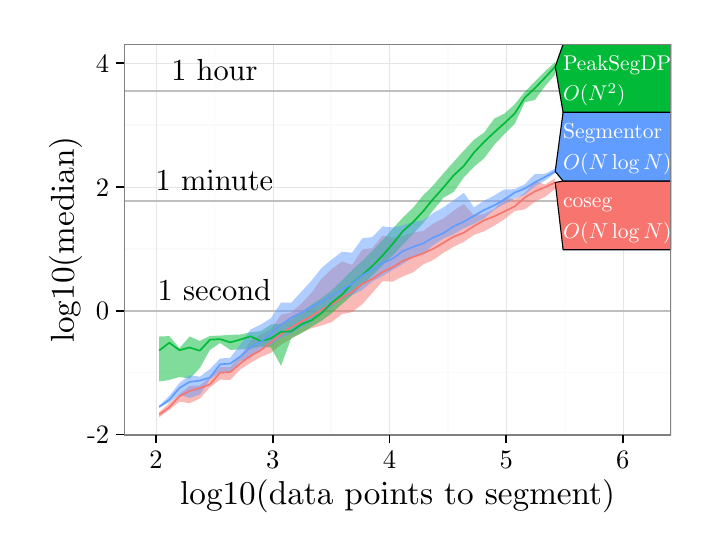
\begin{tikzpicture}[x=1pt,y=1pt]
\definecolor[named]{fillColor}{rgb}{1.00,1.00,1.00}
\path[use as bounding box,fill=fillColor,fill opacity=0.00] (0,0) rectangle (238.49,180.67);
\begin{scope}
\path[clip] (  0.00,  0.00) rectangle (238.49,180.67);
\definecolor[named]{drawColor}{rgb}{1.00,1.00,1.00}
\definecolor[named]{fillColor}{rgb}{1.00,1.00,1.00}

\path[draw=drawColor,line width= 0.6pt,line join=round,line cap=round,fill=fillColor] (  0.00,  0.00) rectangle (238.49,180.68);
\end{scope}
\begin{scope}
\path[clip] ( 34.86, 33.48) rectangle (232.49,174.67);
\definecolor[named]{fillColor}{rgb}{1.00,1.00,1.00}

\path[fill=fillColor] ( 34.86, 33.48) rectangle (232.49,174.67);
\definecolor[named]{drawColor}{rgb}{0.98,0.98,0.98}

\path[draw=drawColor,line width= 0.6pt,line join=round] ( 34.86, 56.02) --
	(232.49, 56.02);

\path[draw=drawColor,line width= 0.6pt,line join=round] ( 34.86,100.74) --
	(232.49,100.74);

\path[draw=drawColor,line width= 0.6pt,line join=round] ( 34.86,145.46) --
	(232.49,145.46);

\path[draw=drawColor,line width= 0.6pt,line join=round] ( 67.48, 33.48) --
	( 67.48,174.67);

\path[draw=drawColor,line width= 0.6pt,line join=round] (109.65, 33.48) --
	(109.65,174.67);

\path[draw=drawColor,line width= 0.6pt,line join=round] (151.82, 33.48) --
	(151.82,174.67);

\path[draw=drawColor,line width= 0.6pt,line join=round] (193.99, 33.48) --
	(193.99,174.67);
\definecolor[named]{drawColor}{rgb}{0.90,0.90,0.90}

\path[draw=drawColor,line width= 0.2pt,line join=round] ( 34.86, 33.66) --
	(232.49, 33.66);

\path[draw=drawColor,line width= 0.2pt,line join=round] ( 34.86, 78.38) --
	(232.49, 78.38);

\path[draw=drawColor,line width= 0.2pt,line join=round] ( 34.86,123.10) --
	(232.49,123.10);

\path[draw=drawColor,line width= 0.2pt,line join=round] ( 34.86,167.81) --
	(232.49,167.81);

\path[draw=drawColor,line width= 0.2pt,line join=round] ( 46.40, 33.48) --
	( 46.40,174.67);

\path[draw=drawColor,line width= 0.2pt,line join=round] ( 88.57, 33.48) --
	( 88.57,174.67);

\path[draw=drawColor,line width= 0.2pt,line join=round] (130.74, 33.48) --
	(130.74,174.67);

\path[draw=drawColor,line width= 0.2pt,line join=round] (172.90, 33.48) --
	(172.90,174.67);

\path[draw=drawColor,line width= 0.2pt,line join=round] (215.07, 33.48) --
	(215.07,174.67);
\definecolor[named]{drawColor}{rgb}{0.75,0.75,0.75}
\definecolor[named]{fillColor}{rgb}{0.75,0.75,0.75}

\path[draw=drawColor,line width= 0.6pt,line join=round,fill=fillColor] ( 34.86, 78.38) -- (232.49, 78.38);

\path[draw=drawColor,line width= 0.6pt,line join=round,fill=fillColor] ( 34.86,118.14) -- (232.49,118.14);

\path[draw=drawColor,line width= 0.6pt,line join=round,fill=fillColor] ( 34.86,157.89) -- (232.49,157.89);
\definecolor[named]{fillColor}{rgb}{0.97,0.46,0.43}

\path[fill=fillColor,fill opacity=0.50] ( 47.52, 41.75) --
	( 51.18, 44.96) --
	( 54.85, 48.27) --
	( 58.52, 51.22) --
	( 62.19, 51.38) --
	( 65.86, 54.33) --
	( 69.53, 58.03) --
	( 73.20, 58.03) --
	( 76.87, 62.05) --
	( 80.54, 67.50) --
	( 84.21, 69.75) --
	( 87.88, 71.67) --
	( 91.55, 76.97) --
	( 95.22, 77.72) --
	( 98.89, 80.98) --
	(102.56, 84.85) --
	(106.23, 89.99) --
	(109.90, 93.44) --
	(113.57, 96.18) --
	(117.24, 94.96) --
	(120.91,100.47) --
	(124.57,101.04) --
	(128.24,105.52) --
	(131.91,104.84) --
	(135.58,105.37) --
	(139.25,106.66) --
	(142.92,107.20) --
	(146.59,109.91) --
	(150.26,111.72) --
	(153.93,114.58) --
	(157.60,116.98) --
	(161.27,112.75) --
	(164.94,113.33) --
	(168.61,115.17) --
	(172.28,119.26) --
	(175.95,118.62) --
	(179.62,120.85) --
	(183.29,125.29) --
	(186.96,124.01) --
	(190.63,126.28) --
	(190.63,122.39) --
	(186.96,119.52) --
	(183.29,117.74) --
	(179.62,115.01) --
	(175.95,114.40) --
	(172.28,111.47) --
	(168.61,109.13) --
	(164.94,107.10) --
	(161.27,105.79) --
	(157.60,103.26) --
	(153.93,101.53) --
	(150.26, 99.34) --
	(146.59, 96.78) --
	(142.92, 95.11) --
	(139.25, 92.25) --
	(135.58, 90.82) --
	(131.91, 88.90) --
	(128.24, 89.08) --
	(124.57, 84.85) --
	(120.91, 80.73) --
	(117.24, 77.89) --
	(113.57, 77.18) --
	(109.90, 74.30) --
	(106.23, 73.06) --
	(102.56, 72.05) --
	( 98.89, 70.43) --
	( 95.22, 68.24) --
	( 91.55, 66.12) --
	( 87.88, 63.18) --
	( 84.21, 61.62) --
	( 80.54, 59.56) --
	( 76.87, 57.21) --
	( 73.20, 53.36) --
	( 69.53, 53.48) --
	( 65.86, 50.73) --
	( 62.19, 46.63) --
	( 58.52, 44.96) --
	( 54.85, 45.55) --
	( 51.18, 42.56) --
	( 47.52, 39.89) --
	cycle;
\definecolor[named]{fillColor}{rgb}{0.00,0.73,0.22}

\path[fill=fillColor,fill opacity=0.50] ( 47.52, 69.06) --
	( 51.18, 69.21) --
	( 54.85, 64.88) --
	( 58.52, 69.09) --
	( 62.19, 67.47) --
	( 65.86, 69.26) --
	( 69.53, 69.41) --
	( 73.20, 69.67) --
	( 76.87, 69.77) --
	( 80.54, 70.63) --
	( 84.21, 70.99) --
	( 87.88, 73.39) --
	( 91.55, 73.67) --
	( 95.22, 75.20) --
	( 98.89, 77.82) --
	(102.56, 80.59) --
	(106.23, 82.94) --
	(109.90, 85.77) --
	(113.57, 89.38) --
	(117.24, 93.04) --
	(120.91, 96.45) --
	(124.57,100.05) --
	(128.24,103.82) --
	(131.91,108.06) --
	(135.58,112.05) --
	(139.25,115.58) --
	(142.92,120.10) --
	(146.59,123.74) --
	(150.26,128.05) --
	(153.93,132.18) --
	(157.60,136.25) --
	(161.27,140.19) --
	(164.94,142.77) --
	(168.61,147.82) --
	(172.28,149.62) --
	(175.95,152.94) --
	(179.62,157.48) --
	(183.29,161.24) --
	(186.96,164.94) --
	(190.63,168.26) --
	(190.63,163.71) --
	(186.96,159.54) --
	(183.29,154.55) --
	(179.62,153.71) --
	(175.95,145.85) --
	(172.28,142.19) --
	(168.61,138.37) --
	(164.94,133.45) --
	(161.27,130.38) --
	(157.60,126.58) --
	(153.93,121.29) --
	(150.26,119.22) --
	(146.59,114.75) --
	(142.92,110.04) --
	(139.25,106.16) --
	(135.58,102.31) --
	(131.91, 98.42) --
	(128.24, 94.79) --
	(124.57, 91.19) --
	(120.91, 87.71) --
	(117.24, 84.03) --
	(113.57, 80.78) --
	(109.90, 77.50) --
	(106.23, 74.80) --
	(102.56, 72.57) --
	( 98.89, 70.25) --
	( 95.22, 68.46) --
	( 91.55, 58.49) --
	( 87.88, 65.11) --
	( 84.21, 65.48) --
	( 80.54, 64.68) --
	( 76.87, 64.40) --
	( 73.20, 64.23) --
	( 69.53, 66.69) --
	( 65.86, 64.23) --
	( 62.19, 57.63) --
	( 58.52, 53.85) --
	( 54.85, 54.44) --
	( 51.18, 53.36) --
	( 47.52, 52.83) --
	cycle;
\definecolor[named]{fillColor}{rgb}{0.38,0.61,1.00}

\path[fill=fillColor,fill opacity=0.50] ( 47.52, 44.00) --
	( 51.18, 47.60) --
	( 54.85, 52.28) --
	( 58.52, 55.10) --
	( 62.19, 54.56) --
	( 65.86, 57.29) --
	( 69.53, 61.12) --
	( 73.20, 61.40) --
	( 76.87, 66.19) --
	( 80.54, 71.61) --
	( 84.21, 73.39) --
	( 87.88, 75.66) --
	( 91.55, 81.34) --
	( 95.22, 81.25) --
	( 98.89, 85.29) --
	(102.56, 89.29) --
	(106.23, 93.87) --
	(109.90, 96.92) --
	(113.57, 99.71) --
	(117.24, 99.35) --
	(120.91,104.51) --
	(124.57,105.01) --
	(128.24,108.86) --
	(131.91,108.48) --
	(135.58,109.24) --
	(139.25,110.47) --
	(142.92,111.07) --
	(146.59,113.71) --
	(150.26,115.75) --
	(153.93,118.30) --
	(157.60,121.01) --
	(161.27,115.74) --
	(164.94,118.17) --
	(168.61,120.04) --
	(172.28,122.26) --
	(175.95,122.29) --
	(179.62,124.07) --
	(183.29,127.84) --
	(186.96,127.86) --
	(190.63,129.76) --
	(190.63,128.12) --
	(186.96,125.40) --
	(183.29,123.34) --
	(179.62,120.27) --
	(175.95,118.95) --
	(172.28,116.97) --
	(168.61,114.86) --
	(164.94,111.79) --
	(161.27,109.82) --
	(157.60,108.16) --
	(153.93,106.03) --
	(150.26,104.48) --
	(146.59,102.09) --
	(142.92, 98.90) --
	(139.25, 97.76) --
	(135.58, 95.25) --
	(131.91, 93.15) --
	(128.24, 90.91) --
	(124.57, 89.00) --
	(120.91, 85.89) --
	(117.24, 84.09) --
	(113.57, 82.55) --
	(109.90, 79.55) --
	(106.23, 77.59) --
	(102.56, 74.27) --
	( 98.89, 72.36) --
	( 95.22, 70.18) --
	( 91.55, 68.51) --
	( 87.88, 65.88) --
	( 84.21, 64.56) --
	( 80.54, 61.40) --
	( 76.87, 60.21) --
	( 73.20, 56.21) --
	( 69.53, 56.31) --
	( 65.86, 53.61) --
	( 62.19, 48.05) --
	( 58.52, 46.88) --
	( 54.85, 48.05) --
	( 51.18, 45.26) --
	( 47.52, 43.31) --
	cycle;
\definecolor[named]{drawColor}{rgb}{0.97,0.46,0.43}

\path[draw=drawColor,line width= 0.6pt,line join=round] ( 47.52, 40.87) --
	( 51.18, 43.48) --
	( 54.85, 47.48) --
	( 58.52, 49.39) --
	( 62.19, 50.39) --
	( 65.86, 51.76) --
	( 69.53, 56.02) --
	( 73.20, 56.21) --
	( 76.87, 59.36) --
	( 80.54, 62.10) --
	( 84.21, 64.09) --
	( 87.88, 66.94) --
	( 91.55, 69.91) --
	( 95.22, 72.43) --
	( 98.89, 74.48) --
	(102.56, 76.42) --
	(106.23, 78.75) --
	(109.90, 80.73) --
	(113.57, 83.09) --
	(117.24, 85.14) --
	(120.91, 88.10) --
	(124.57, 89.86) --
	(128.24, 92.39) --
	(131.91, 94.08) --
	(135.58, 96.39) --
	(139.25, 97.79) --
	(142.92, 99.12) --
	(146.59,100.79) --
	(150.26,102.96) --
	(153.93,105.16) --
	(157.60,106.58) --
	(161.27,108.99) --
	(164.94,111.08) --
	(168.61,112.49) --
	(172.28,114.29) --
	(175.95,116.05) --
	(179.62,119.25) --
	(183.29,121.52) --
	(186.96,123.02) --
	(190.63,124.72);
\definecolor[named]{drawColor}{rgb}{0.00,0.73,0.22}

\path[draw=drawColor,line width= 0.6pt,line join=round] ( 47.52, 64.00) --
	( 51.18, 66.83) --
	( 54.85, 64.11) --
	( 58.52, 65.11) --
	( 62.19, 63.94) --
	( 65.86, 67.90) --
	( 69.53, 68.14) --
	( 73.20, 66.94) --
	( 76.87, 67.99) --
	( 80.54, 69.14) --
	( 84.21, 67.39) --
	( 87.88, 68.38) --
	( 91.55, 70.78) --
	( 95.22, 70.89) --
	( 98.89, 73.50) --
	(102.56, 74.93) --
	(106.23, 77.59) --
	(109.90, 81.30) --
	(113.57, 84.17) --
	(117.24, 88.30) --
	(120.91, 91.24) --
	(124.57, 94.61) --
	(128.24, 98.31) --
	(131.91,102.56) --
	(135.58,107.14) --
	(139.25,110.39) --
	(142.92,114.34) --
	(146.59,118.84) --
	(150.26,122.92) --
	(153.93,127.31) --
	(157.60,130.71) --
	(161.27,135.54) --
	(164.94,139.39) --
	(168.61,142.87) --
	(172.28,146.16) --
	(175.95,149.60) --
	(179.62,155.37) --
	(183.29,158.82) --
	(186.96,162.65) --
	(190.63,166.59);
\definecolor[named]{drawColor}{rgb}{0.38,0.61,1.00}

\path[draw=drawColor,line width= 0.6pt,line join=round] ( 47.52, 43.66) --
	( 51.18, 46.23) --
	( 54.85, 50.48) --
	( 58.52, 52.70) --
	( 62.19, 53.10) --
	( 65.86, 54.27) --
	( 69.53, 59.01) --
	( 73.20, 59.29) --
	( 76.87, 61.84) --
	( 80.54, 65.19) --
	( 84.21, 67.12) --
	( 87.88, 70.06) --
	( 91.55, 73.29) --
	( 95.22, 75.84) --
	( 98.89, 77.70) --
	(102.56, 79.75) --
	(106.23, 81.55) --
	(109.90, 83.78) --
	(113.57, 86.07) --
	(117.24, 88.11) --
	(120.91, 91.09) --
	(124.57, 93.32) --
	(128.24, 95.55) --
	(131.91, 97.24) --
	(135.58, 99.93) --
	(139.25,101.45) --
	(142.92,102.71) --
	(146.59,104.86) --
	(150.26,106.42) --
	(153.93,108.86) --
	(157.60,110.53) --
	(161.27,112.68) --
	(164.94,114.80) --
	(168.61,116.45) --
	(172.28,118.61) --
	(175.95,121.09) --
	(179.62,122.53) --
	(183.29,124.79) --
	(186.96,126.72) --
	(190.63,128.73);
\definecolor[named]{drawColor}{rgb}{0.00,0.00,0.00}

\node[text=drawColor,anchor=base,inner sep=0pt, outer sep=0pt, scale=  1.10] at ( 67.48, 82.18) {1 second};

\node[text=drawColor,anchor=base,inner sep=0pt, outer sep=0pt, scale=  1.10] at ( 67.48,121.94) {1 minute};

\node[text=drawColor,anchor=base,inner sep=0pt, outer sep=0pt, scale=  1.10] at ( 67.48,161.70) {1 hour};
\end{scope}
\begin{scope}
\path[clip] ( 34.86, 33.48) rectangle (232.49,174.67);
\definecolor[named]{drawColor}{rgb}{0.00,0.00,0.00}
\definecolor[named]{fillColor}{rgb}{0.97,0.46,0.43}

\path[draw=drawColor,line width= 0.4pt,line join=round,line cap=round,fill=fillColor] (190.63,124.72) --
	(193.47,125.26) --
	(232.49,125.26) --
	(232.49,100.44) --
	(193.47,100.44) --
	cycle;
\definecolor[named]{fillColor}{rgb}{0.38,0.61,1.00}

\path[draw=drawColor,line width= 0.4pt,line join=round,line cap=round,fill=fillColor] (190.63,128.73) --
	(193.47,150.09) --
	(232.49,150.09) --
	(232.49,125.26) --
	(193.47,125.26) --
	cycle;
\definecolor[named]{fillColor}{rgb}{0.00,0.73,0.22}

\path[draw=drawColor,line width= 0.4pt,line join=round,line cap=round,fill=fillColor] (190.63,166.59) --
	(193.47,174.67) --
	(232.49,174.67) --
	(232.49,150.09) --
	(193.47,150.09) --
	cycle;
\definecolor[named]{drawColor}{rgb}{1.00,1.00,1.00}

\node[text=drawColor,anchor=base west,inner sep=0pt, outer sep=0pt, scale=  0.78] at (193.47,115.77) {coseg};

\node[text=drawColor,anchor=base west,inner sep=0pt, outer sep=0pt, scale=  0.78] at (193.47,104.57) {$O(N \log N)$};

\node[text=drawColor,anchor=base west,inner sep=0pt, outer sep=0pt, scale=  0.78] at (193.47,140.60) {Segmentor};

\node[text=drawColor,anchor=base west,inner sep=0pt, outer sep=0pt, scale=  0.78] at (193.47,129.40) {$O(N \log N)$};

\node[text=drawColor,anchor=base west,inner sep=0pt, outer sep=0pt, scale=  0.77] at (193.47,165.28) {PeakSegDP};

\node[text=drawColor,anchor=base west,inner sep=0pt, outer sep=0pt, scale=  0.77] at (193.47,154.19) {$O(N^2)$};
\definecolor[named]{drawColor}{rgb}{0.50,0.50,0.50}

\path[draw=drawColor,line width= 0.6pt,line join=round,line cap=round] ( 34.86, 33.48) rectangle (232.49,174.67);
\end{scope}
\begin{scope}
\path[clip] (  0.00,  0.00) rectangle (238.49,180.67);
\definecolor[named]{drawColor}{rgb}{0.00,0.00,0.00}

\node[text=drawColor,anchor=base east,inner sep=0pt, outer sep=0pt, scale=  0.96] at ( 29.46, 30.36) {-2};

\node[text=drawColor,anchor=base east,inner sep=0pt, outer sep=0pt, scale=  0.96] at ( 29.46, 75.07) {0};

\node[text=drawColor,anchor=base east,inner sep=0pt, outer sep=0pt, scale=  0.96] at ( 29.46,119.79) {2};

\node[text=drawColor,anchor=base east,inner sep=0pt, outer sep=0pt, scale=  0.96] at ( 29.46,164.51) {4};
\end{scope}
\begin{scope}
\path[clip] (  0.00,  0.00) rectangle (238.49,180.67);
\definecolor[named]{drawColor}{rgb}{0.00,0.00,0.00}

\path[draw=drawColor,line width= 0.6pt,line join=round] ( 31.86, 33.66) --
	( 34.86, 33.66);

\path[draw=drawColor,line width= 0.6pt,line join=round] ( 31.86, 78.38) --
	( 34.86, 78.38);

\path[draw=drawColor,line width= 0.6pt,line join=round] ( 31.86,123.10) --
	( 34.86,123.10);

\path[draw=drawColor,line width= 0.6pt,line join=round] ( 31.86,167.81) --
	( 34.86,167.81);
\end{scope}
\begin{scope}
\path[clip] (  0.00,  0.00) rectangle (238.49,180.67);
\definecolor[named]{drawColor}{rgb}{0.00,0.00,0.00}

\path[draw=drawColor,line width= 0.6pt,line join=round] ( 46.40, 30.48) --
	( 46.40, 33.48);

\path[draw=drawColor,line width= 0.6pt,line join=round] ( 88.57, 30.48) --
	( 88.57, 33.48);

\path[draw=drawColor,line width= 0.6pt,line join=round] (130.74, 30.48) --
	(130.74, 33.48);

\path[draw=drawColor,line width= 0.6pt,line join=round] (172.90, 30.48) --
	(172.90, 33.48);

\path[draw=drawColor,line width= 0.6pt,line join=round] (215.07, 30.48) --
	(215.07, 33.48);
\end{scope}
\begin{scope}
\path[clip] (  0.00,  0.00) rectangle (238.49,180.67);
\definecolor[named]{drawColor}{rgb}{0.00,0.00,0.00}

\node[text=drawColor,anchor=base,inner sep=0pt, outer sep=0pt, scale=  0.96] at ( 46.40, 21.46) {2};

\node[text=drawColor,anchor=base,inner sep=0pt, outer sep=0pt, scale=  0.96] at ( 88.57, 21.46) {3};

\node[text=drawColor,anchor=base,inner sep=0pt, outer sep=0pt, scale=  0.96] at (130.74, 21.46) {4};

\node[text=drawColor,anchor=base,inner sep=0pt, outer sep=0pt, scale=  0.96] at (172.90, 21.46) {5};

\node[text=drawColor,anchor=base,inner sep=0pt, outer sep=0pt, scale=  0.96] at (215.07, 21.46) {6};
\end{scope}
\begin{scope}
\path[clip] (  0.00,  0.00) rectangle (238.49,180.67);
\definecolor[named]{drawColor}{rgb}{0.00,0.00,0.00}

\node[text=drawColor,anchor=base,inner sep=0pt, outer sep=0pt, scale=  1.20] at (133.68,  8.40) {log10(data points to segment)};
\end{scope}
\begin{scope}
\path[clip] (  0.00,  0.00) rectangle (238.49,180.67);
\definecolor[named]{drawColor}{rgb}{0.00,0.00,0.00}

\node[text=drawColor,rotate= 90.00,anchor=base,inner sep=0pt, outer sep=0pt, scale=  1.20] at ( 16.66,104.08) {log10(median)};
\end{scope}
\end{tikzpicture}

  }
  \caption{Left: number of intervals stored by the algorithm, Right: timings in seconds}
  \label{fig:timings}
\end{figure}

\bibliographystyle{abbrvnat}
\bibliography{refs}

\end{document}

